% Options for packages loaded elsewhere
\PassOptionsToPackage{unicode}{hyperref}
\PassOptionsToPackage{hyphens}{url}
\PassOptionsToPackage{dvipsnames,svgnames,x11names}{xcolor}
%
\documentclass[
  letterpaper,
  DIV=11,
  numbers=noendperiod]{scrreprt}

\usepackage{amsmath,amssymb}
\usepackage{iftex}
\ifPDFTeX
  \usepackage[T1]{fontenc}
  \usepackage[utf8]{inputenc}
  \usepackage{textcomp} % provide euro and other symbols
\else % if luatex or xetex
  \usepackage{unicode-math}
  \defaultfontfeatures{Scale=MatchLowercase}
  \defaultfontfeatures[\rmfamily]{Ligatures=TeX,Scale=1}
\fi
\usepackage{lmodern}
\ifPDFTeX\else  
    % xetex/luatex font selection
\fi
% Use upquote if available, for straight quotes in verbatim environments
\IfFileExists{upquote.sty}{\usepackage{upquote}}{}
\IfFileExists{microtype.sty}{% use microtype if available
  \usepackage[]{microtype}
  \UseMicrotypeSet[protrusion]{basicmath} % disable protrusion for tt fonts
}{}
\makeatletter
\@ifundefined{KOMAClassName}{% if non-KOMA class
  \IfFileExists{parskip.sty}{%
    \usepackage{parskip}
  }{% else
    \setlength{\parindent}{0pt}
    \setlength{\parskip}{6pt plus 2pt minus 1pt}}
}{% if KOMA class
  \KOMAoptions{parskip=half}}
\makeatother
\usepackage{xcolor}
\setlength{\emergencystretch}{3em} % prevent overfull lines
\setcounter{secnumdepth}{5}
% Make \paragraph and \subparagraph free-standing
\makeatletter
\ifx\paragraph\undefined\else
  \let\oldparagraph\paragraph
  \renewcommand{\paragraph}{
    \@ifstar
      \xxxParagraphStar
      \xxxParagraphNoStar
  }
  \newcommand{\xxxParagraphStar}[1]{\oldparagraph*{#1}\mbox{}}
  \newcommand{\xxxParagraphNoStar}[1]{\oldparagraph{#1}\mbox{}}
\fi
\ifx\subparagraph\undefined\else
  \let\oldsubparagraph\subparagraph
  \renewcommand{\subparagraph}{
    \@ifstar
      \xxxSubParagraphStar
      \xxxSubParagraphNoStar
  }
  \newcommand{\xxxSubParagraphStar}[1]{\oldsubparagraph*{#1}\mbox{}}
  \newcommand{\xxxSubParagraphNoStar}[1]{\oldsubparagraph{#1}\mbox{}}
\fi
\makeatother

\usepackage{color}
\usepackage{fancyvrb}
\newcommand{\VerbBar}{|}
\newcommand{\VERB}{\Verb[commandchars=\\\{\}]}
\DefineVerbatimEnvironment{Highlighting}{Verbatim}{commandchars=\\\{\}}
% Add ',fontsize=\small' for more characters per line
\usepackage{framed}
\definecolor{shadecolor}{RGB}{241,243,245}
\newenvironment{Shaded}{\begin{snugshade}}{\end{snugshade}}
\newcommand{\AlertTok}[1]{\textcolor[rgb]{0.68,0.00,0.00}{#1}}
\newcommand{\AnnotationTok}[1]{\textcolor[rgb]{0.37,0.37,0.37}{#1}}
\newcommand{\AttributeTok}[1]{\textcolor[rgb]{0.40,0.45,0.13}{#1}}
\newcommand{\BaseNTok}[1]{\textcolor[rgb]{0.68,0.00,0.00}{#1}}
\newcommand{\BuiltInTok}[1]{\textcolor[rgb]{0.00,0.23,0.31}{#1}}
\newcommand{\CharTok}[1]{\textcolor[rgb]{0.13,0.47,0.30}{#1}}
\newcommand{\CommentTok}[1]{\textcolor[rgb]{0.37,0.37,0.37}{#1}}
\newcommand{\CommentVarTok}[1]{\textcolor[rgb]{0.37,0.37,0.37}{\textit{#1}}}
\newcommand{\ConstantTok}[1]{\textcolor[rgb]{0.56,0.35,0.01}{#1}}
\newcommand{\ControlFlowTok}[1]{\textcolor[rgb]{0.00,0.23,0.31}{\textbf{#1}}}
\newcommand{\DataTypeTok}[1]{\textcolor[rgb]{0.68,0.00,0.00}{#1}}
\newcommand{\DecValTok}[1]{\textcolor[rgb]{0.68,0.00,0.00}{#1}}
\newcommand{\DocumentationTok}[1]{\textcolor[rgb]{0.37,0.37,0.37}{\textit{#1}}}
\newcommand{\ErrorTok}[1]{\textcolor[rgb]{0.68,0.00,0.00}{#1}}
\newcommand{\ExtensionTok}[1]{\textcolor[rgb]{0.00,0.23,0.31}{#1}}
\newcommand{\FloatTok}[1]{\textcolor[rgb]{0.68,0.00,0.00}{#1}}
\newcommand{\FunctionTok}[1]{\textcolor[rgb]{0.28,0.35,0.67}{#1}}
\newcommand{\ImportTok}[1]{\textcolor[rgb]{0.00,0.46,0.62}{#1}}
\newcommand{\InformationTok}[1]{\textcolor[rgb]{0.37,0.37,0.37}{#1}}
\newcommand{\KeywordTok}[1]{\textcolor[rgb]{0.00,0.23,0.31}{\textbf{#1}}}
\newcommand{\NormalTok}[1]{\textcolor[rgb]{0.00,0.23,0.31}{#1}}
\newcommand{\OperatorTok}[1]{\textcolor[rgb]{0.37,0.37,0.37}{#1}}
\newcommand{\OtherTok}[1]{\textcolor[rgb]{0.00,0.23,0.31}{#1}}
\newcommand{\PreprocessorTok}[1]{\textcolor[rgb]{0.68,0.00,0.00}{#1}}
\newcommand{\RegionMarkerTok}[1]{\textcolor[rgb]{0.00,0.23,0.31}{#1}}
\newcommand{\SpecialCharTok}[1]{\textcolor[rgb]{0.37,0.37,0.37}{#1}}
\newcommand{\SpecialStringTok}[1]{\textcolor[rgb]{0.13,0.47,0.30}{#1}}
\newcommand{\StringTok}[1]{\textcolor[rgb]{0.13,0.47,0.30}{#1}}
\newcommand{\VariableTok}[1]{\textcolor[rgb]{0.07,0.07,0.07}{#1}}
\newcommand{\VerbatimStringTok}[1]{\textcolor[rgb]{0.13,0.47,0.30}{#1}}
\newcommand{\WarningTok}[1]{\textcolor[rgb]{0.37,0.37,0.37}{\textit{#1}}}

\providecommand{\tightlist}{%
  \setlength{\itemsep}{0pt}\setlength{\parskip}{0pt}}\usepackage{longtable,booktabs,array}
\usepackage{calc} % for calculating minipage widths
% Correct order of tables after \paragraph or \subparagraph
\usepackage{etoolbox}
\makeatletter
\patchcmd\longtable{\par}{\if@noskipsec\mbox{}\fi\par}{}{}
\makeatother
% Allow footnotes in longtable head/foot
\IfFileExists{footnotehyper.sty}{\usepackage{footnotehyper}}{\usepackage{footnote}}
\makesavenoteenv{longtable}
\usepackage{graphicx}
\makeatletter
\newsavebox\pandoc@box
\newcommand*\pandocbounded[1]{% scales image to fit in text height/width
  \sbox\pandoc@box{#1}%
  \Gscale@div\@tempa{\textheight}{\dimexpr\ht\pandoc@box+\dp\pandoc@box\relax}%
  \Gscale@div\@tempb{\linewidth}{\wd\pandoc@box}%
  \ifdim\@tempb\p@<\@tempa\p@\let\@tempa\@tempb\fi% select the smaller of both
  \ifdim\@tempa\p@<\p@\scalebox{\@tempa}{\usebox\pandoc@box}%
  \else\usebox{\pandoc@box}%
  \fi%
}
% Set default figure placement to htbp
\def\fps@figure{htbp}
\makeatother

\KOMAoption{captions}{tableheading}
\makeatletter
\@ifpackageloaded{bookmark}{}{\usepackage{bookmark}}
\makeatother
\makeatletter
\@ifpackageloaded{caption}{}{\usepackage{caption}}
\AtBeginDocument{%
\ifdefined\contentsname
  \renewcommand*\contentsname{Table of contents}
\else
  \newcommand\contentsname{Table of contents}
\fi
\ifdefined\listfigurename
  \renewcommand*\listfigurename{List of Figures}
\else
  \newcommand\listfigurename{List of Figures}
\fi
\ifdefined\listtablename
  \renewcommand*\listtablename{List of Tables}
\else
  \newcommand\listtablename{List of Tables}
\fi
\ifdefined\figurename
  \renewcommand*\figurename{Figure}
\else
  \newcommand\figurename{Figure}
\fi
\ifdefined\tablename
  \renewcommand*\tablename{Table}
\else
  \newcommand\tablename{Table}
\fi
}
\@ifpackageloaded{float}{}{\usepackage{float}}
\floatstyle{ruled}
\@ifundefined{c@chapter}{\newfloat{codelisting}{h}{lop}}{\newfloat{codelisting}{h}{lop}[chapter]}
\floatname{codelisting}{Listing}
\newcommand*\listoflistings{\listof{codelisting}{List of Listings}}
\makeatother
\makeatletter
\makeatother
\makeatletter
\@ifpackageloaded{caption}{}{\usepackage{caption}}
\@ifpackageloaded{subcaption}{}{\usepackage{subcaption}}
\makeatother

\usepackage{bookmark}

\IfFileExists{xurl.sty}{\usepackage{xurl}}{} % add URL line breaks if available
\urlstyle{same} % disable monospaced font for URLs
\hypersetup{
  pdftitle={Probability And Business Statistics},
  pdfauthor={Pamela Schlosser},
  colorlinks=true,
  linkcolor={blue},
  filecolor={Maroon},
  citecolor={Blue},
  urlcolor={Blue},
  pdfcreator={LaTeX via pandoc}}


\title{Probability And Business Statistics}
\author{Pamela Schlosser}
\date{2026-04-15}

\begin{document}
\maketitle

\renewcommand*\contentsname{Table of contents}
{
\hypersetup{linkcolor=}
\setcounter{tocdepth}{2}
\tableofcontents
}

\bookmarksetup{startatroot}

\chapter{Module 0: Software Know-How}\label{module-0-software-know-how}

\bookmarksetup{startatroot}

\chapter{Why R?}\label{why-r}

\begin{itemize}
\item
  In an OMSBA Probability and Statistics course, we teach R because it
  is a powerful, flexible tool widely used in business analytics for
  data analysis and visualization. R allows students to apply
  theoretical concepts to real-world datasets, enhancing their
  understanding through hands-on practice. Its rich ecosystem of
  packages, like ggplot2 for visualization and dplyr for data
  manipulation, makes it ideal for tackling the types of problems
  analysts face in the field. Additionally, R promotes reproducibility
  and collaboration through features like R Markdown and RStudio
  Projects, which align with industry standards. By learning R, students
  not only gain valuable technical skills but also build a strong
  foundation for advanced analytics and decision-making in their
  careers.
\item
  R is a mature, industry-standard statistical language used across
  academia, healthcare, finance, and data science. R scripts document
  exactly what was done to the data --- making your analysis
  reproducible, auditable, and gradable.
\item
  Easily installed, state-of-the-art, and it is free and open source and
  supported by a well-established R Community.
\item
  R can be used with RStudio, which is a graphical user interface that
  allows you to do the following:

  \begin{itemize}
  \tightlist
  \item
    write, edit, and execute code;
  \item
    generate, view, and store plots;
  \item
    manage files, objects and data frames;
  \item
    integrate with version control systems.
  \end{itemize}
\item
  This R Community helps in the development of R resources

  \begin{itemize}
  \tightlist
  \item
    A package is developed by R users to do one specific thing or a set
    of related things that could store a collection of functions, data,
    and code.
  \item
    A library is the place where the package is located on your
    computer.
  \item
    A repository is a central location where many developed packages are
    located and available for download. There are 3 big repositories,
    but we use Comprehensive R Archive Network, or CRAN, which is R's
    main repository with over 223,596 packages available.
  \end{itemize}
\end{itemize}

\bookmarksetup{startatroot}

\chapter{Installing R}\label{installing-r}

\section{Installing R on Windows}\label{installing-r-on-windows}

\begin{itemize}
\tightlist
\item
  Open an internet browser and go to \url{https://www.r-project.org/}.
\item
  Click CRAN hyperlink underneath Download on the left.
\item
  Select a CRAN location (a mirror site) and click the corresponding
  link. I selected O-cloud. This brings you to the following link:
  \url{https://cloud.r-project.org/}
\item
  Click on the ``Download R for Windows'' link at the top of the page if
  you have a Windows computer.\\
\item
  Click on the ``install R for the first time'' link at the top of the
  page.
\item
  Click ``Download R for Windows'' and save the executable file
  somewhere on your computer.
\item
  Run the .exe file
\item
  Accept all defaults and follow the installation instructions
\item
  Now that R is installed, you need to download and install RStudio.
\end{itemize}

\section{Installing R on a Mac}\label{installing-r-on-a-mac}

\begin{itemize}
\tightlist
\item
  Open an internet browser and go to \url{https://www.r-project.org/}.
\item
  Click CRAN hyperlink underneath Download on the left.
\item
  Select a CRAN location (a mirror site) and click the corresponding
  link. I selected O-cloud. This brings you to the following link:
  \url{https://cloud.r-project.org/}
\item
  Click on the ``Download R for (Mac) OS X'' link at the top of the
  page.
\item
  Click on the file containing the latest version of R under ``Files.''
\item
  Save the .pkg file, double-click it to open, and follow the
  installation instructions.
\item
  Accept the license agreement and all subsequent defaults
\item
  When the installation completes, click Close.
\item
  Now that R is installed, you need to download and install RStudio.
\end{itemize}

\bookmarksetup{startatroot}

\chapter{Installing R Studio}\label{installing-r-studio}

\section{Downloading RStudio For Mac or
PC}\label{downloading-rstudio-for-mac-or-pc}

\begin{itemize}
\tightlist
\item
  Go to the following URL:
  \url{https://posit.co/download/rstudio-desktop/}.
\item
  Click the Download button for Install RStudio.
\item
  It should recognize your operating system. If you see different an
  Installers for Supported Platforms section, click the version that is
  appropriate for your operating system. When the download is complete,
  run the install program, accepting all defaults.
\item
  Note, RStudio might conflict with some Mac antivirus programs. Ensure
  your antivirus is not blocking it from installing. Only worry about
  this if you have difficulty installing the program.
\end{itemize}

\begin{figure}[H]

{\centering \pandocbounded{\includegraphics[keepaspectratio]{Pictures/Ch0/RStudio.png}}

}

\caption{RStudio}

\end{figure}%

\bookmarksetup{startatroot}

\chapter{Take Your First Look at R}\label{take-your-first-look-at-r}

\begin{itemize}
\tightlist
\item
  On the right, two windows, each with tabs

  \begin{itemize}
  \tightlist
  \item
    There are many ways to customize the look of RStudio for
    accessibility purposes with a couple being the following:

    \begin{itemize}
    \tightlist
    \item
      You can resize the windows using the splitters.
    \item
      You can maximize/restore the windows within the left/right panels
      using the familiar Windows controls in the upper-right of each
      window.
    \end{itemize}
  \end{itemize}
\item
  On the left, the Console Window reproduces the R environment.

  \begin{itemize}
  \tightlist
  \item
    Observe the command line with the \(>\) symbol.
  \end{itemize}
\end{itemize}

\begin{figure}[H]

{\centering \pandocbounded{\includegraphics[keepaspectratio]{Pictures/Ch0/Console.png}}

}

\caption{Console}

\end{figure}%

\bookmarksetup{startatroot}

\chapter{Project Files}\label{project-files}

\begin{itemize}
\tightlist
\item
  A RStudio project is a way to organize your work by creating a
  self-contained environment for your files, scripts, and outputs.

  \begin{itemize}
  \tightlist
  \item
    The RStudio project file sits in the root directory, with the
    extension .Rproj.
  \item
    When your RStudio session is running through the project file
    (.Rproj), the current working directory points to the root folder
    where that .Rproj file is saved.
  \end{itemize}
\item
  Key Features

  \begin{itemize}
  \tightlist
  \item
    Keeps all related files in one folder.
  \item
    Automatically sets the working directory to the project folder.
  \item
    Simplifies managing file paths (``data/myfile.csv'' instead of a
    full path).
  \end{itemize}
\end{itemize}

\begin{itemize}
\tightlist
\item
  Creating a project for our class. Projects are great because they aid
  in your organization technique.
\item
  You will find that some professors are not insistent on making a
  project for their class, but it is helpful to still do to organize
  your materials. You will have a lot of code in this program!
\item
  To create a project click
  \(File > New Project - New Directory > New Project\) and save your
  project to a place on your computer (not the cloud).
\end{itemize}

\begin{figure}[H]

{\centering \pandocbounded{\includegraphics[keepaspectratio]{Pictures/Ch0/CreateProject.png}}

}

\caption{CreateProject}

\end{figure}%

\bookmarksetup{startatroot}

\chapter{R Script files}\label{r-script-files}

\begin{itemize}
\tightlist
\item
  Entering and running code at the R command line is effective and
  simple. However, each time you want to execute a set of commands, you
  have to re-enter them at the command line. Nothing saves for later.
\item
  Complex commands are particularly difficult causing you to re-entering
  the code to fix any errors typographical or otherwise. Fortunately,
  you can make a .R script file to solve this issue.
\item
  A .R script is simply a text file containing a set of commands and
  comments. The script can be saved and used later to rerun the code.
  The script can also be documented with comments and edited again and
  again to suit your needs.\\
\item
  Create your first R Script file within your Project for testing
  purposes.

  \begin{itemize}
  \tightlist
  \item
    Go to File \textgreater{} New File \textgreater{} R Script
  \item
    Save this file as MyFirstRscript.R in your project folder you just
    made. You should see this new file under Files like mine is in the
    bottom right panel. As we create new files, continue to save them
    into your project folder.
  \end{itemize}
\item
  On the .R file presented to the left, comments are added as denoted by
  the hashtag which you can type or push ctrl + shift + c.
\item
  If you type in your console, it will not save it for later. However,
  if you save code in this R Script file, you can open your file at a
  later date to rerun your code. Also, as we move through the class,
  feel free to document all your notes in your .R file via \# called
  comments. More on comments later.
\end{itemize}

\begin{figure}[H]

{\centering \pandocbounded{\includegraphics[keepaspectratio]{Pictures/Ch0/MyFirstScript.png}}

}

\caption{Screenshot of MyFirstScript.R}

\end{figure}%

\bookmarksetup{startatroot}

\chapter{Using R More Effectively}\label{using-r-more-effectively}

\section{Customizing RStudio}\label{customizing-rstudio}

\begin{itemize}
\tightlist
\item
  Customizing RStudio through global options allows you to create a
  coding environment that aligns with your workflow and personal
  preferences. By tailoring settings such as appearance, pane layout,
  and editor behavior, you can improve productivity, enhance
  readability, and streamline your data analysis process. These
  adjustments not only make coding more efficient but also help you
  avoid common pitfalls, like workspace clutter or inconsistent
  settings. RStudio is highly flexible, so take the time to explore and
  experiment with its options to make the platform work best for you.
\end{itemize}

\begin{itemize}
\tightlist
\item
  What are Global Options

  \begin{itemize}
  \tightlist
  \item
    Settings in RStudio that let you personalize the environment to suit
    your workflow.
  \end{itemize}
\item
  Why change global options?

  \begin{itemize}
  \tightlist
  \item
    Improve productivity by tailoring RStudio to your preferences.
  \item
    Enhance readability and usability of code and outputs.
  \item
    Create a consistent environment across projects.
  \end{itemize}
\item
  Where to Find Global Options:

  \begin{itemize}
  \tightlist
  \item
    Go to Tools \textgreater{} Global Options in the RStudio menu.
  \end{itemize}
\item
  Key Settings to Adjust

  \begin{itemize}
  \tightlist
  \item
    Global Options \textgreater{} General: You can set your general
    information including your default working directory (when not in a
    project).Set your R Version if appropriate.
  \item
    Global Options \textgreater{} Code: Enable auto-complete, or
    soft-wrap for easier coding.
  \item
    Global Options \textgreater{} Appearance: You can customize the
    appearance to a theme that accommodates your learning style and
    visual preferences.
  \item
    Global Options \textgreater{} Spelling: You can turn on a spell
    check.
  \end{itemize}
\end{itemize}

\begin{figure}[H]

{\centering \pandocbounded{\includegraphics[keepaspectratio]{Pictures/Ch0/Options.png}}

}

\caption{Tools \textgreater{} Global Options.R}

\end{figure}%

\section{Quick Keys in R}\label{quick-keys-in-r}

\begin{itemize}
\tightlist
\item
  There are a lot of quick keys in R to make you able to use it faster
  and more effectively. You may look over these and try on your own.
\end{itemize}

\begin{figure}[H]

{\centering \pandocbounded{\includegraphics[keepaspectratio]{Pictures/Ch0/QuickKeys1.png}}

}

\caption{Console Quick Keys}

\end{figure}%%
\begin{figure}[H]

{\centering \pandocbounded{\includegraphics[keepaspectratio]{Pictures/Ch0/QuickKeys2.png}}

}

\caption{Source Quick Keys}

\end{figure}%%
\begin{figure}[H]

{\centering \pandocbounded{\includegraphics[keepaspectratio]{Pictures/Ch0/QuickKeys3.png}}

}

\caption{Editing Quick Keys}

\end{figure}%

\section{Getting Help in R}\label{getting-help-in-r}

\begin{itemize}
\tightlist
\item
  There are lots of ways to get help in R.
\item
  In R, use the help search box to find information on a function,
  parameter, or package.

  \begin{itemize}
  \tightlist
  \item
    ?mean
  \item
    help.search(`swirl')
  \item
    help(package = `MASS')
  \item
    ?install.packages
  \end{itemize}
\end{itemize}

\begin{figure}[H]

{\centering \pandocbounded{\includegraphics[keepaspectratio]{Pictures/Ch0/Help.png}}

}

\caption{Getting Help}

\end{figure}%

\begin{itemize}
\tightlist
\item
  You should try to look up the tapply command to see what it does.

  \begin{itemize}
  \tightlist
  \item
    Use ?tapply in your .R file to pull up tapply() command or type
    tapply in the Help box. * Formally, you should see that the command
    applies a function to each cell of a ragged array, that is to each
    (non-empty) group of values given by a unique combination of the
    levels of certain factors. This means that the command does some
    math calculation (mean, sum, etc.) on a continuous variable after
    dividing the data by group.
  \end{itemize}
\item
  The format is tapply(x, index, and fun), where x is a continuous
  variable, index is a grouping variable or factor, and fun is a
  function like mean.
\item
  More on that function later in the first lessons.
\end{itemize}

\bookmarksetup{startatroot}

\chapter{Accessing Data Files for the
Course}\label{accessing-data-files-for-the-course}

\begin{itemize}
\tightlist
\item
  To download the data sets, go to our Canvas datasets page and download
  them to your computer
\item
  Once downloaded, unzip the file by right-clicking and selecting
  ``Extract All'', and then move the subfolder named data to your
  working directory.
\item
  In the example below, my project folder for the class is called
  BUAD512A and the subfolder that contains all the data files is called
  data. You can put your folder anywhere on the hard drive of your
  computer, but do not download it to places on the cloud like OneDrive.
\end{itemize}

\begin{figure}[H]

{\centering \pandocbounded{\includegraphics[keepaspectratio]{Pictures/Ch0/BookFiles.png}}

}

\caption{Saving Our Book Files Into a ``data'' Folder in Your Working
Directory}

\end{figure}%

\begin{itemize}
\tightlist
\item
  We will use a number of data files plus more for homework/projects, so
  be prepared to use these files throughout the class.
\end{itemize}

\bookmarksetup{startatroot}

\chapter{Introduction to RMarkdown}\label{introduction-to-rmarkdown}

\begin{itemize}
\tightlist
\item
  R Markdown (RMD) files are a versatile format that combines plain
  text, code, and output to create dynamic and reproducible documents.
\item
  Benefits of Using RMD Files:

  \begin{itemize}
  \tightlist
  \item
    Reproducibility: Combining code and output ensures that the document
    is reproducible. Any changes in the data or analysis can be quickly
    updated.
  \item
    Integration: RMD files seamlessly integrate with R, allowing you to
    run and display results from your analysis within the same document.
  \item
    Flexibility: You can produce various types of reports, including
    static documents and dynamic documents.
  \item
    Collaboration: Being that RMD files are plain text, they are easy to
    share and version control with tools like Git.
  \end{itemize}
\item
  RMD files have many options, but generally are composed of the
  following:

  \begin{itemize}
  \tightlist
  \item
    yaml Header
  \item
    markdown Text
  \item
    Code Chunks
  \item
    Output Formats
  \item
    Visualization and Plots
  \end{itemize}
\end{itemize}

\section{yaml Header}\label{yaml-header}

\begin{itemize}
\tightlist
\item
  The YAML header is located at the beginning of the RMD file and
  contains metadata about the document, such as the title, author, date,
  and output format. Here is an example of a YAML header:
\end{itemize}

\begin{figure}[H]

{\centering \pandocbounded{\includegraphics[keepaspectratio]{Pictures/Ch0/ymlHeader.png}}

}

\caption{YAML Header Example}

\end{figure}%

\section{markdown Text}\label{markdown-text}

\begin{itemize}
\tightlist
\item
  Markdown is a lightweight markup language with plain text formatting
  syntax. In an RMD file, you use Markdown to format the text, create
  lists, headers, links, and more. For example:
\end{itemize}

\begin{figure}[H]

{\centering \pandocbounded{\includegraphics[keepaspectratio]{Pictures/RMD/markdownStyles.png}}

}

\caption{Styles Example}

\end{figure}%

\section{Code Chunks}\label{code-chunks}

\begin{itemize}
\tightlist
\item
  Code chunks allow you to embed R (or other languages) code within the
  document. These chunks are executed when the document is rendered, and
  their output is included in the final document. Code chunks are
  defined with triple backticks and the language, like this:
\end{itemize}

\begin{figure}[H]

{\centering \pandocbounded{\includegraphics[keepaspectratio]{Pictures/RMD/codechunk.png}}

}

\caption{Code Chunk Example}

\end{figure}%

\begin{itemize}
\tightlist
\item
  Chunk output can be customized with knitr options, arguments set in
  the \{\} of a chunk header.

  \begin{itemize}
  \tightlist
  \item
    include = FALSE prevents code and results from appearing in the
    finished file. R Markdown still runs the code in the chunk, and the
    results can be used by other chunks.
  \item
    echo = FALSE prevents code, but not the results from appearing in
    the finished file. This is a useful way to embed figures.
  \item
    message = FALSE prevents messages that are generated by code from
    appearing in the finished file.
  \item
    warning = FALSE prevents warnings that are generated by code from
    appearing in the finished.
  \item
    fig.cap = ``\ldots{}'' adds a caption to graphical results.
  \end{itemize}
\end{itemize}

\begin{figure}[H]

{\centering \pandocbounded{\includegraphics[keepaspectratio]{Pictures/RMD/message.png}}

}

\caption{Arguments of Chunk}

\end{figure}%

\section{Output Formats}\label{output-formats}

\begin{itemize}
\tightlist
\item
  RMD files can be rendered into various output formats including HTML,
  PDF, and Word documents. The output format is specified in the YAML
  header. To generate the final document, you use the knit function in
  RStudio or call rmarkdown::render() in your R script.
\end{itemize}

\section{Visualization and Plots}\label{visualization-and-plots}

\begin{itemize}
\tightlist
\item
  RMD files can include visualizations and plots. For example, you can
  create and embed a plot using the ggplot2 package.
\end{itemize}

library(ggplot2) ggplot(mpg, aes(x=displ, y=hwy)) + geom\_point()

\begin{Shaded}
\begin{Highlighting}[]
\FunctionTok{library}\NormalTok{(ggplot2)}
\FunctionTok{ggplot}\NormalTok{(mpg, }\FunctionTok{aes}\NormalTok{(}\AttributeTok{x=}\NormalTok{displ, }\AttributeTok{y=}\NormalTok{hwy)) }\SpecialCharTok{+} \FunctionTok{geom\_point}\NormalTok{()}
\end{Highlighting}
\end{Shaded}

\pandocbounded{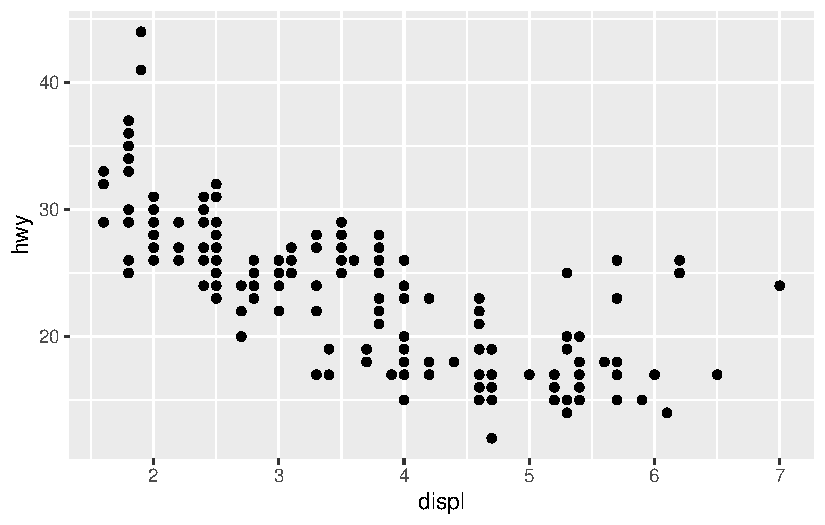
\includegraphics[keepaspectratio]{index_files/figure-pdf/unnamed-chunk-1-1.pdf}}

\section{Using RMD for Homework}\label{using-rmd-for-homework}

\begin{itemize}
\item
  You will be asked to edit an RMarkdown (.Rmd) file to process your R
  assignments in this course. This requires you to answer the assignment
  questions in .R and copy your answer to the appropriate R chunk in the
  .Rmd file, or answer the questions directly in the .Rmd file. To
  complete this process successfully, follow these steps:

  \begin{itemize}
  \tightlist
  \item
    A .Rmd file will be linked on each applicable assignment page in
    Canvas. These files contain the instructions for each individual the
    assessment. Using RStudio, open the .Rmd file (which can be
    downloaded from Canvas into your working directory).
  \item
    Inside the .Rmd file, you will see R chunks. This is where you will
    put your answers. Do not delete the \ldots\{r\} or the \ldots{} at
    the end of the chunk. Those characters signifies what type of chunk
    you have (an R chunk) and needs beginning characters and closing
    characters to work.
  \item
    Once you complete your tasks, select knit to make the .pdf file.
  \item
    After you knit, you can find the .pdf file in your working
    directory. You can open it to verify that all of your answers are
    included.
  \item
    If your .Rmd file won't knit, you should submit your .Rmd file
    instead of the .pdf file. While this will cost you points on the
    assignment, it will still allow your instructor to evaluate the rest
    of the code.
  \end{itemize}
\end{itemize}

\section{Packages Required for RMD to
Work}\label{packages-required-for-rmd-to-work}

\begin{itemize}
\tightlist
\item
  RMarkdown requires updated packages for formatting and when saving as
  .pdf documents, a latex extension is also required so that it properly
  reads the formulas in the problems. Download the .R file on Canvas and
  follow the instructions provided to use RMarkdown. You may also watch
  the tutorial video on Canvas for specific information on how to set up
  R Markdown Files.
\end{itemize}

\begin{figure}[H]

{\centering \pandocbounded{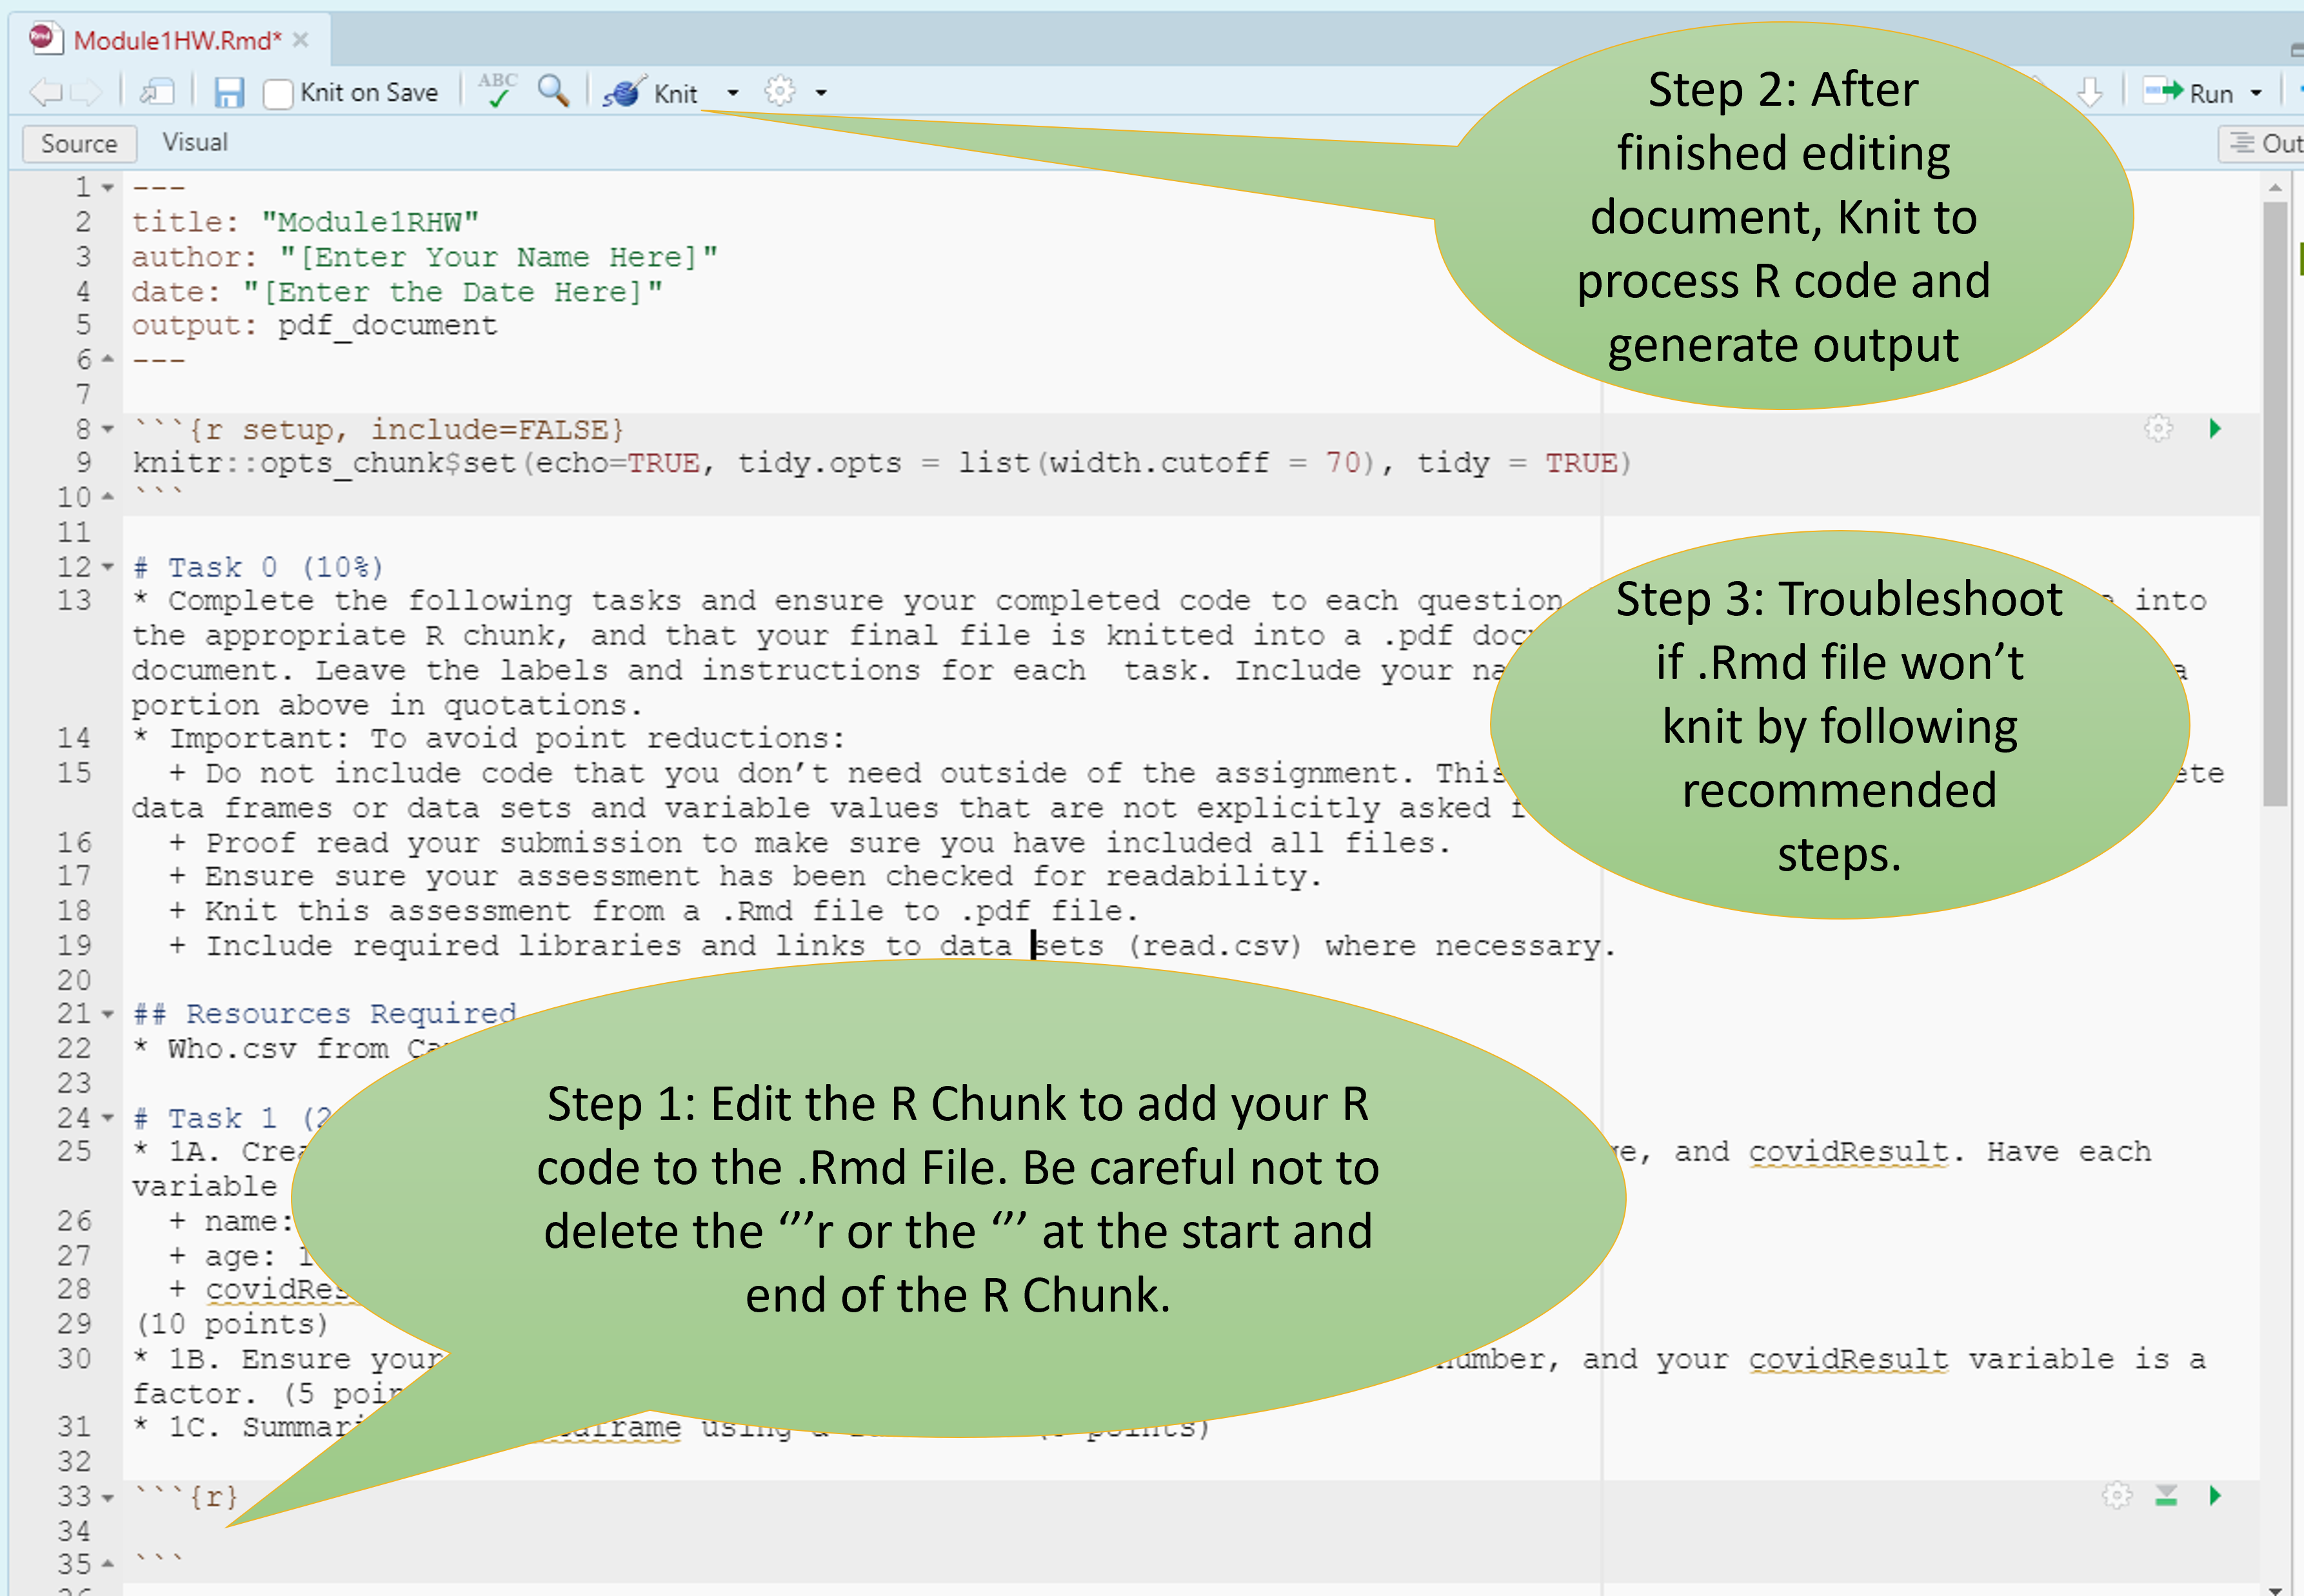
\includegraphics[keepaspectratio]{Pictures/RMD/RMDTasks.png}}

}

\caption{Looking at the HW}

\end{figure}%

\begin{itemize}
\tightlist
\item
  To use RMarkdown most efficiently, make sure your version of R is the
  latest by checking the website. If it is not, then take the time to
  get the latest version of the software. Second, make sure your files
  are not on the cloud, including OneDrive. If so, then decouple at
  least your desktop with OneDrive so you can work off the cloud.
  Finally, run the lines below one at a time. Once the packages are done
  installing, then restart your computer. Finally, open RStudio and run
  a blank RMarkdown file. If this file knits, then your homework should
  knit as long as there are no other errors.
\end{itemize}

\begin{Shaded}
\begin{Highlighting}[]
\FunctionTok{install.packages}\NormalTok{(}\StringTok{"rmarkdown"}\NormalTok{)}
\FunctionTok{install.packages}\NormalTok{(}\StringTok{"knitr"}\NormalTok{)}
\FunctionTok{install.packages}\NormalTok{(}\StringTok{"formatR"}\NormalTok{)}
\NormalTok{tinytex}\SpecialCharTok{::}\FunctionTok{install\_tinytex}\NormalTok{()  }\CommentTok{\# Select Y when/if it asks down in the console.}
\end{Highlighting}
\end{Shaded}

\begin{itemize}
\item
  You may only need to update one of these packages. However, since they
  are all connected, running these commands ensures that they are all up
  to date with minimal troubleshooting.
\item
  If you are having difficulty knitting to pdf, feel free to publish it
  in a .html and print the .html to a .pdf. I just ask that the final
  uploaded document with answers be a pdf. To do this, click the drop
  down arrow on the Knit option and select Knit to HTML.
\end{itemize}

\section{Troubleshooting RMD FIles}\label{troubleshooting-rmd-files}

\begin{itemize}
\item
  The videos on Canvas offer a walk through of how to use RMD files
  successfully in this course. Understanding how to use RMD files is
  essential to your success on assignments in this course. Please note
  that these videos will not show you the specific homework questions or
  specific answers. The files you will see in the following videos are
  for demonstration purposes only. Course homework assignments change
  regularly, so the specific contents of the files shown in the videos
  will likely differ from those you will see for your assignments.
\item
  Lack of Syntax Errors:

  \begin{itemize}
  \tightlist
  \item
    R Markdown files may fail to knit without providing clear syntax
    error messages.
  \item
    To troubleshoot, run each code chunk interactively in RStudio to
    identify and fix errors before knitting.
  \item
    Pay attention to any warnings or messages in the console as they may
    indicate potential issues.
  \end{itemize}
\item
  Using Relative Links to Datasets:

  \begin{itemize}
  \tightlist
  \item
    If the .Rmd file relies on external datasets, ensure that file paths
    are specified using relative links.
  \item
    Relative links ensure portability, allowing the .Rmd file to work on
    different systems without modification.
  \item
    For example, if a dataset is in a subfolder, use a path like data
    \textless- read.csv(``data/my\_dataset.csv'').
  \item
    Always verify that the dataset exists in the specified location
    relative to the working directory.
  \end{itemize}
\item
  Including Necessary Libraries:

  \begin{itemize}
  \tightlist
  \item
    Functions from external libraries will fail if the required
    libraries are not loaded.
  \item
    At the beginning of the .Rmd file, load all necessary libraries
    explicitly using library() calls, e.g., library(tidyverse).
  \item
    Ensure that all libraries used in the document are installed
    beforehand by running install.packages() if needed.
  \item
    Loading libraries early prevents errors during knitting and avoids
    confusing error messages.
  \end{itemize}
\end{itemize}

\bookmarksetup{startatroot}

\chapter{Summary}\label{summary}

\begin{itemize}
\tightlist
\item
  At the end of this section, you should have downloaded and browsed R
  in RStudio. You should have looked at the quick keys in R to make
  editing your R documents easier. You should set up a project folder
  for the course where you want to on your computer, and made your first
  .R script file located in that project folder. You should have tried a
  line of code or two as presented. Finally, you should have looked
  around the RStudio environment and found the help tab.
\end{itemize}

\bookmarksetup{startatroot}

\chapter{Module 1: Introduction to R and
RStudio}\label{module-1-introduction-to-r-and-rstudio}

\begin{itemize}
\tightlist
\item
  The goal of this lesson is to introduce you to R and RStudio while
  teaching you how to perform data preparation using these tools. In
  this part, we will go over forming an understanding of statistics,
  learning about observations and variables, and being able to move
  around and get comfortable with R. I will also teach you how use and
  load data.
\end{itemize}

\subsection{At a Glance}\label{at-a-glance}

\begin{itemize}
\tightlist
\item
  In order to succeed in this lesson, you will need to start by having
  both R and RStudio downloaded. Then, the only way to learn R is to use
  it in various ways and to practice as much as you can.
\item
  It is also important to note that this is a statistics class and that
  R is a statistical computing software. Because of that, we need to not
  only pay attention to what we are typing in, but understand why we are
  typing it in the ways suggested, and also how we could do it
  differently to get similar if not the same results.
\end{itemize}

\subsection{Lesson Objectives}\label{lesson-objectives}

\begin{itemize}
\tightlist
\item
  Be Introduced to R and R Studio.
\item
  Set up R and R Studio.
\item
  Use basic Built-in Functions in R.
\item
  Enter and load data into R.
\end{itemize}

\subsection{Consider While Reading}\label{consider-while-reading}

\begin{itemize}
\tightlist
\item
  This material is so important because it is likely the start of your R
  journey and will provide the groundwork for learning a modern approach
  to calculating statistics. R has a fairly steep learning curve, but,
  once you are over it, it becomes fairly easy to figure out new things.
  It is important to make connections to what we are doing and why we
  are doing it a certain way. There are rules to learning R, and you
  will get better with constant practice. Try to avoid just typing in
  code. Instead, determine why the code was typed the way it was and try
  to figure out all the other ways the code could also be typed to get
  the same answer. Practice, practice, practice!
\end{itemize}

\section{What is Statistics?}\label{what-is-statistics}

\begin{itemize}
\tightlist
\item
  Statistics is the methodology of extracting useful information from a
  data set.
\item
  Numerical results are not very useful unless they are accompanied with
  clearly stated actionable business insights.
\item
  To do good statistical analysis, you must do the following:

  \begin{itemize}
  \tightlist
  \item
    Find the right data.
  \item
    Use the appropriate statistical tools.
  \item
    Clearly communicate the numerical information in written language.
  \end{itemize}
\item
  With knowledge of statistics:

  \begin{itemize}
  \tightlist
  \item
    Avoid risk of making uninformed decisions and costly mistakes.
  \item
    Differentiate between sound statistical conclusions and questionable
    conclusions.
  \end{itemize}
\item
  Data and analytics capabilities have made a leap forward.

  \begin{itemize}
  \tightlist
  \item
    Growing availability of vast amounts of data.
  \item
    Improved computational power.
  \item
    Development of sophisticated algorithms.
  \item
    The rise of Generative AI.
  \end{itemize}
\end{itemize}

\subsection{Definition of AI}\label{definition-of-ai}

\begin{itemize}
\tightlist
\item
  Artificial Intelligence (AI) is the development of computer systems
  that can perform tasks that typically require human intelligence ---
  things like recognizing patterns, making decisions, understanding
  language, and generating content.
\item
  For the purposes of this course, the most relevant category is
  generative AI (tools like ChatGPT, Claude, and GitHub Copilot), which
  can produce text, code, and analysis in response to natural language
  prompts.
\end{itemize}

\subsection{Two Main Branches of
Statistics}\label{two-main-branches-of-statistics}

\begin{itemize}
\tightlist
\item
  Descriptive Statistics - collecting, organizing, and presenting the
  data.
\item
  Inferential Statistics - drawing conclusions about a population based
  on sample data from that population.

  \begin{itemize}
  \tightlist
  \item
    A population consists of all items of interest.
  \item
    A sample is a subset of the population.
  \item
    A sample statistic is calculated from the sample data and is used to
    make inferences about the population parameter.
  \end{itemize}
\item
  Reasons for sampling from the population:

  \begin{itemize}
  \tightlist
  \item
    Too expensive to gather information on the entire population.
  \item
    Often impossible to gather information on the entire population.
  \end{itemize}
\end{itemize}

\subsubsection{Descriptive Statistics and
AI}\label{descriptive-statistics-and-ai}

\begin{itemize}
\tightlist
\item
  Descriptive Statistics is where AI currently dominates. Tools like
  ChatGPT, Copilot, and R's own AI-assisted packages can collect data
  via APIs, clean and wrangle it, generate summary statistics, and
  produce polished visualizations faster than any human. When you ask AI
  to ``summarize this dataset,'' it's doing descriptive work. The output
  is only as good as the data fed in, but the mechanical execution is
  largely automated.
\end{itemize}

\subsubsection{Inferential Statistics and
AI}\label{inferential-statistics-and-ai}

\begin{itemize}
\tightlist
\item
  Inferential Statistics is where human judgment remains essential, and
  AI actually introduces new complications. Consider:

  \begin{itemize}
  \tightlist
  \item
    Who defines the population? If you're studying customer behavior, do
    you mean all customers, all potential customers, all customers in a
    region? AI won't ask this question --- it will answer whatever you
    give it. Defining the population of interest is a business and
    conceptual judgment call, not a computation.
  \item
    Is the sample representative? AI can run a regression or t-test in
    seconds, but it cannot tell you whether your sample was collected
    with selection bias, convenience sampling, or missing key subgroups.
    That requires domain knowledge and critical thinking.
  \item
    What do the inferences actually mean? A p-value of 0.03 in a
    business context means something different from one in a clinical
    trial. Translating statistical conclusions into actionable decisions
    --- and communicating uncertainty honestly to a non-technical
    audience --- is still entirely a human skill.
  \end{itemize}
\end{itemize}

\subsection{Reasons for sampling from the
population}\label{reasons-for-sampling-from-the-population}

\begin{itemize}
\tightlist
\item
  Too expensive to gather information on the entire population.
\item
  Often impossible to gather information on the entire population.
\item
  AI models are themselves built on samples --- no training dataset
  captures all human knowledge, all languages, or all possible
  situations. This is why AI has blind spots, biases, and confidently
  wrong answers. The same sampling limitations we study in this course
  apply directly to the tools you use every day.
\end{itemize}

\subsection{AI vs.~Statistics}\label{ai-vs.-statistics}

\begin{itemize}
\tightlist
\item
  Statistics is a branch of mathematics focused on collecting,
  analyzing, and interpreting data under uncertainty. AI systems,
  particularly modern ones, are largely built on statistical methods ---
  machine learning models are essentially very complex statistical
  models trained on large datasets. So, statistics isn't separate from
  AI; it's foundational to it.
\item
  AI vs.~Machine Learning --- Machine learning is a subset of AI where
  systems learn from data rather than being explicitly programmed with
  rules. Most of what powers tools like ChatGPT falls here.
\item
  AI vs.~a calculator --- A calculator executes exactly what you tell
  it. An AI system infers, predicts, and generates --- which makes it
  more powerful and also less predictable. It can be wrong with great
  confidence.
\end{itemize}

\subsection{R Comes with Assistance}\label{r-comes-with-assistance}

\begin{itemize}
\tightlist
\item
  R's community is vast, and you can always seek information from the
  community to try to help you with a R related issue.
\item
  AI tools like ChatGPT and GitHub Copilot can also assist with R syntax
  and debugging --- but the analyst must understand, verify, and take
  ownership of every line of code submitted.
\end{itemize}

\subsection{R is Called a Dynamically Typed
Language}\label{r-is-called-a-dynamically-typed-language}

R figures out a variable's data type automatically based on whatever you
assign to it. You can change it, but you don't have to declare it
upfront like in some other languages.

\subsection{What makes you fluent in R --- with or without
AI:}\label{what-makes-you-fluent-in-r-with-or-without-ai}

\begin{itemize}
\tightlist
\item
  Troubleshooting (AI helps, but you must read the error)
\item
  The Environment --- AI can assist if you share your context, but you
  must know what to share and why
\item
  Assignment operator
\item
  Sequences
\item
  Built-in functions
\item
  Reading data
\item
  Packages
\item
  Conditional statements
\item
  Rendering output
\item
  Writing functions
\item
  Prompting and verifying AI-generated code
\end{itemize}

\bookmarksetup{startatroot}

\chapter{Setting up R}\label{setting-up-r}

\section{R Script Files}\label{r-script-files-1}

\begin{itemize}
\tightlist
\item
  Using R Script Files:

  \begin{itemize}
  \tightlist
  \item
    A .R script is simply a text file containing a set of commands and
    comments. The script can be saved and used later to rerun the code.
    The script can also be documented with comments and edited again and
    again to suit your needs.
  \end{itemize}
\item
  Using the Console

  \begin{itemize}
  \tightlist
  \item
    Entering and running code at the R command line is effective and
    simple. However, each time you want to execute a set of commands,
    you must re-enter them at the command line. Nothing saves for later.
  \end{itemize}
\item
  Complex commands are particularly difficult, forcing you to re-enter
  the code to fix any errors --- typographical or otherwise. R script
  files help to solve this issue.
\end{itemize}

\subsection{Create a New R Script
File}\label{create-a-new-r-script-file}

\begin{itemize}
\tightlist
\item
  To save your notes from this lesson, create a .R file named module1.R
  and save it to your project file you made in the last class.
\item
  There are a couple of parts to this module, and we can add code for
  the entire module in one file so that our code is stacked nicely
  together.\\
\item
  For each new module, start a new file and save it to your project
  folder.
\end{itemize}

\begin{figure}[H]

{\centering \pandocbounded{\includegraphics[keepaspectratio]{Pictures/Ch1/RScript.png}}

}

\caption{Screenshot of R Environment}

\end{figure}%

\bookmarksetup{startatroot}

\chapter{Using R}\label{using-r}

\section{Text in R}\label{text-in-r}

\subsection{Comments}\label{comments}

\begin{itemize}
\item
  Use comments to organize and explain your code in R scripts by
  including 1 or more than 1 hashtag.
\item
  Aim to write clear, self-explanatory code that minimizes the need for
  excessive comments.
\item
  Add helpful comments where necessary to ensure anyone, including your
  future self, can understand and run the code.
\item
  If something doesn't work, avoid deleting it immediately. Instead,
  comment it out while troubleshooting or exploring alternatives.
\item
  Essentially, we add comments to our code to document our work and add
  notes to our self or to others.
\end{itemize}

\begin{Shaded}
\begin{Highlighting}[]
\CommentTok{\# This is a comment for documentation or annotation}
\end{Highlighting}
\end{Shaded}

\begin{itemize}
\tightlist
\item
  Add the code above to your R file and run each line using Ctl + Enter
  (PC) or Cmd + Return (MAC) or select all lines and click Run.
\item
  Take note that nothing prints in the console after running a comment.
\end{itemize}

\subsection{A Prolog}\label{a-prolog}

\begin{itemize}
\tightlist
\item
  A prolog is a set of comments at the top of a code file that provides
  information about what is in the file. It also names the files and
  resources used that facilitates identification. Including a prolog is
  considered coding best practice.
\item
  On your own R Script File, add your own prolog following the template
  as shown.
\item
  An informal prolog is below:
\end{itemize}

\begin{Shaded}
\begin{Highlighting}[]
\DocumentationTok{\#\#\#\#\#\#\#\#\#\#\#\#\#\#\#\#\#\#\#\#\#\#\#\#\#\#\#\#\#\#\#\#\#\#\#\#}
\CommentTok{\# Project name: Module 1}
\CommentTok{\# Project purpose: To create an R script file to learn about R. }
\CommentTok{\# Code author name: [Enter Your Name]}
\CommentTok{\# Date last edited: [Enter Date Here]}
\CommentTok{\# Data used: NA}
\CommentTok{\# Libraries used: NA}
\DocumentationTok{\#\#\#\#\#\#\#\#\#\#\#\#\#\#\#\#\#\#\#\#\#\#\#\#\#\#\#\#\#\#\#\#\#\#\#\#}
\end{Highlighting}
\end{Shaded}

\begin{itemize}
\tightlist
\item
  Then, as we work through our .R script and add data files or libraries
  to our code, we go back and edit the prolog.
\end{itemize}

\begin{figure}[H]

{\centering \pandocbounded{\includegraphics[keepaspectratio]{Pictures/Ch1/Chapter1Start.png}}

}

\caption{Chapter 1 R File}

\end{figure}%

\subsection{String}\label{string}

\begin{itemize}
\tightlist
\item
  In R, a \emph{string} is a sequence of characters enclosed in quotes,
  used to represent text data.
\item
  R accepts single quotes or double quotes when marking a \emph{string}.
  However, if you use a single quote to start, use a single quote to
  end. The same for double quotes - ensure the pairing is the same quote
  type.
\item
  You sometimes need to be careful with nested quotes, but generally it
  does not matter which you use.
\end{itemize}

\begin{Shaded}
\begin{Highlighting}[]
\StringTok{"This is a string"}
\end{Highlighting}
\end{Shaded}

\begin{verbatim}
[1] "This is a string"
\end{verbatim}

\begin{Shaded}
\begin{Highlighting}[]
\StringTok{"This is also a string"}
\end{Highlighting}
\end{Shaded}

\begin{verbatim}
[1] "This is also a string"
\end{verbatim}

\section{Note on R Markdown}\label{note-on-r-markdown}

\begin{itemize}
\tightlist
\item
  These files were formatted with RMarkdown. RMarkdown is a simple
  formatting syntax for authoring documents of a variety of types,
  including PowerPoint and html files.
\item
  On the document, RMarkdown prints the command and then follows the
  command with the output after 2 hashtags.
\item
  In your R Script File, you only need to type in the command and then
  run your code to get the same output as presented here.
\end{itemize}

\begin{figure}[H]

{\centering \pandocbounded{\includegraphics[keepaspectratio]{Pictures/Ch1/ReadHTML.png}}

}

\caption{Reading our HTML file}

\end{figure}%

\section{Running Commands}\label{running-commands}

\begin{itemize}
\tightlist
\item
  There are a few ways to run commands via your .R file.

  \begin{itemize}
  \tightlist
  \item
    You can click Ctr + Enter on each line (Cmd + Return on a Mac).
  \item
    You can select all the lines you want to run and select Ctr + Enter
    (Cmd + Return on a Mac).
  \item
    You can select all the lines you want to run and select the run
    button as shown in the Figure.
  \end{itemize}
\end{itemize}

\begin{figure}[H]

{\centering \pandocbounded{\includegraphics[keepaspectratio]{Pictures/Ch1/Run.png}}

}

\caption{Run Code}

\end{figure}%

\begin{itemize}
\tightlist
\item
  Now that I have asked you to add a couple lines of code, after this
  point, when R code is shown on this file, you should add it to your .R
  script file along with any notes you want. I won't explicitly say -
  ``add this code.''
\end{itemize}

\section{R is an Interactive
Calculator}\label{r-is-an-interactive-calculator}

\begin{itemize}
\tightlist
\item
  An important facet of R is that it should serve as your sole
  calculator.
\item
  Try these commands in your .R file by typing them in and clicking Ctr
  + Enter on each line for a PC and Cmd + Return on a Mac computer.
\end{itemize}

\begin{Shaded}
\begin{Highlighting}[]
\DecValTok{3} \SpecialCharTok{+} \DecValTok{4}
\end{Highlighting}
\end{Shaded}

\begin{verbatim}
[1] 7
\end{verbatim}

\begin{Shaded}
\begin{Highlighting}[]
\DecValTok{3} \SpecialCharTok{*} \DecValTok{4}
\end{Highlighting}
\end{Shaded}

\begin{verbatim}
[1] 12
\end{verbatim}

\begin{Shaded}
\begin{Highlighting}[]
\DecValTok{3}\SpecialCharTok{/}\DecValTok{4}
\end{Highlighting}
\end{Shaded}

\begin{verbatim}
[1] 0.75
\end{verbatim}

\begin{Shaded}
\begin{Highlighting}[]
\DecValTok{3} \SpecialCharTok{+} \DecValTok{4} \SpecialCharTok{*} \DecValTok{100}\SpecialCharTok{\^{}}\DecValTok{2}
\end{Highlighting}
\end{Shaded}

\begin{verbatim}
[1] 40003
\end{verbatim}

\begin{itemize}
\item
  Take note that order of operations holds in R:
\item
  The order of operations in R, as in mathematics, determines the
  sequence in which expressions are evaluated. This follows the standard
  rules often remembered by the acronym PEMDAS: Parentheses, Exponents,
  Multiplication and Division, and Addition and Subtraction (from left
  to right). Parentheses have the highest precedence and are used to
  group expressions, ensuring they are evaluated first. Operators with
  the same level of precedence, like multiplication and division, are
  evaluated from left to right. When in doubt, use parentheses to make
  the evaluation order explicit and improve the readability of your
  code.

  \begin{itemize}
  \tightlist
  \item
    Parentheses ()
  \item
    Exponents \^{} and \(**\)
  \item
    Division \(/\), Multiplication \(*\), modulo, and integer division
  \item
    Addition + and Subtraction -
  \end{itemize}
\item
  \begin{itemize}
  \tightlist
  \item
    In R, modulo (\%\%) and integer division (\%/\%) also follow the
    order of operations, with both being evaluated after multiplication,
    division, and exponentiation, but before addition and subtraction.
  \end{itemize}
\item
  This means that modulo and integer division have the same priority
  level as multiplication and division, where modulo is just the
  remainder.
\end{itemize}

\begin{Shaded}
\begin{Highlighting}[]
\CommentTok{\# Start with the full expression — what does R see?}
\DecValTok{2} \SpecialCharTok{+} \DecValTok{3} \SpecialCharTok{*} \DecValTok{5} \SpecialCharTok{{-}} \DecValTok{7}\SpecialCharTok{\^{}}\DecValTok{2}\SpecialCharTok{\%\%}\DecValTok{4} \SpecialCharTok{+}\NormalTok{ (}\DecValTok{5}\SpecialCharTok{/}\DecValTok{2}\NormalTok{)}
\end{Highlighting}
\end{Shaded}

\begin{verbatim}
[1] 18.5
\end{verbatim}

\begin{Shaded}
\begin{Highlighting}[]
\CommentTok{\# Step 1: Parentheses first}
\DecValTok{5}\SpecialCharTok{/}\DecValTok{2}  \CommentTok{\# = 2.5}
\end{Highlighting}
\end{Shaded}

\begin{verbatim}
[1] 2.5
\end{verbatim}

\begin{Shaded}
\begin{Highlighting}[]
\CommentTok{\# Expression is now: 2 + 3 * 5 {-} 7\^{}2 \%\% 4 + 2.5}

\CommentTok{\# Step 2: Exponents}
\DecValTok{7}\SpecialCharTok{\^{}}\DecValTok{2}  \CommentTok{\# = 49}
\end{Highlighting}
\end{Shaded}

\begin{verbatim}
[1] 49
\end{verbatim}

\begin{Shaded}
\begin{Highlighting}[]
\CommentTok{\# Expression is now: 2 + 3 * 5 {-} 49 \%\% 4 + 2.5}

\CommentTok{\# Step 3: Multiplication}
\DecValTok{3} \SpecialCharTok{*} \DecValTok{5}  \CommentTok{\# = 15}
\end{Highlighting}
\end{Shaded}

\begin{verbatim}
[1] 15
\end{verbatim}

\begin{Shaded}
\begin{Highlighting}[]
\CommentTok{\# Expression is now: 2 + 15 {-} 49 \%\% 4 + 2.5}

\CommentTok{\# Step 4: Modulo (same level as multiplication/division, left to}
\CommentTok{\# right)}
\DecValTok{49}\SpecialCharTok{\%\%}\DecValTok{4}  \CommentTok{\# = 1  (49 divided by 4 leaves remainder 1)}
\end{Highlighting}
\end{Shaded}

\begin{verbatim}
[1] 1
\end{verbatim}

\begin{Shaded}
\begin{Highlighting}[]
\CommentTok{\# Expression is now: 2 + 15 {-} 1 + 2.5}

\CommentTok{\# Step 5: Addition and subtraction, left to right}
\DecValTok{2} \SpecialCharTok{+} \DecValTok{15}  \CommentTok{\# = 17}
\end{Highlighting}
\end{Shaded}

\begin{verbatim}
[1] 17
\end{verbatim}

\begin{Shaded}
\begin{Highlighting}[]
\DecValTok{17} \SpecialCharTok{{-}} \DecValTok{1}  \CommentTok{\# = 16}
\end{Highlighting}
\end{Shaded}

\begin{verbatim}
[1] 16
\end{verbatim}

\begin{Shaded}
\begin{Highlighting}[]
\DecValTok{16} \SpecialCharTok{+} \FloatTok{2.5}  \CommentTok{\# = 18.5}
\end{Highlighting}
\end{Shaded}

\begin{verbatim}
[1] 18.5
\end{verbatim}

\begin{Shaded}
\begin{Highlighting}[]
\CommentTok{\# Confirm R agrees:}
\FunctionTok{print}\NormalTok{(}\DecValTok{2} \SpecialCharTok{+} \DecValTok{3} \SpecialCharTok{*} \DecValTok{5} \SpecialCharTok{{-}} \DecValTok{7}\SpecialCharTok{\^{}}\DecValTok{2}\SpecialCharTok{\%\%}\DecValTok{4} \SpecialCharTok{+}\NormalTok{ (}\DecValTok{5}\SpecialCharTok{/}\DecValTok{2}\NormalTok{))}
\end{Highlighting}
\end{Shaded}

\begin{verbatim}
[1] 18.5
\end{verbatim}

\begin{Shaded}
\begin{Highlighting}[]
\DocumentationTok{\#\# [1] 18.5}
\end{Highlighting}
\end{Shaded}

\section{Creating Objects}\label{creating-objects}

\begin{itemize}
\tightlist
\item
  Entering and Storing Variables in R requires you to make an
  assignment.

  \begin{itemize}
  \tightlist
  \item
    We use the assignment operator `\textless-' to assign a value or
    expression to a variable.
  \item
    We typically do not use the = sign in R even though it works because
    it also means other things in R.
  \end{itemize}
\item
  Some examples are below to add to your .R file.
\end{itemize}

\begin{Shaded}
\begin{Highlighting}[]
\NormalTok{states }\OtherTok{\textless{}{-}} \DecValTok{29}
\NormalTok{A }\OtherTok{\textless{}{-}} \StringTok{"Apple"}
\CommentTok{\# Equivalent statement to above {-} again = is less used in R.}
\NormalTok{A }\OtherTok{=} \StringTok{"Apple"}
\FunctionTok{print}\NormalTok{(A)}
\end{Highlighting}
\end{Shaded}

\begin{verbatim}
[1] "Apple"
\end{verbatim}

\begin{Shaded}
\begin{Highlighting}[]
\CommentTok{\# Equivalent statement to above}
\NormalTok{A}
\end{Highlighting}
\end{Shaded}

\begin{verbatim}
[1] "Apple"
\end{verbatim}

\begin{Shaded}
\begin{Highlighting}[]
\NormalTok{B }\OtherTok{\textless{}{-}} \DecValTok{3} \SpecialCharTok{+} \DecValTok{4} \SpecialCharTok{*} \DecValTok{12}
\NormalTok{B}
\end{Highlighting}
\end{Shaded}

\begin{verbatim}
[1] 51
\end{verbatim}

\begin{figure}[H]

{\centering \pandocbounded{\includegraphics[keepaspectratio]{Pictures/Ch1/Assignment.png}}

}

\caption{The Assignment Operator}

\end{figure}%

\section{Naming Objects}\label{naming-objects}

\begin{itemize}
\tightlist
\item
  Line length limit: 80
\item
  Always use a consistent way of annotating code.
\item
  \emph{Camel case} is capitalizing the first letter of each word in the
  object name, with the exception of the first word.
\item
  \emph{Dot case} puts a dot between words in a variable name while
  camel case capitalizes each word in the variable name.
\item
  Object names appear on the left of assignment operator. We say an
  object receives or is assigned the value of the expression on the
  right.
\end{itemize}

\begin{enumerate}
\def\labelenumi{\arabic{enumi}.}
\tightlist
\item
  Naming Constants: A Constant contains a single numeric value.
\end{enumerate}

\begin{itemize}
\tightlist
\item
  The \emph{recommended} format for constants is starting with a ``k''
  and then using camel case. (e.g., kStates).
\end{itemize}

\begin{enumerate}
\def\labelenumi{\arabic{enumi}.}
\setcounter{enumi}{1}
\tightlist
\item
  Naming Functions: Functions are objects that perform a series of R
  commands to do something in particular.
\end{enumerate}

\begin{itemize}
\tightlist
\item
  The \emph{recommended} format for Functions is to use Camel case with
  the first letter capitalized. (e.g., MultiplyByTwo).
\end{itemize}

\begin{enumerate}
\def\labelenumi{\arabic{enumi}.}
\setcounter{enumi}{2}
\tightlist
\item
  Naming Variables: A Variable is a measured characteristic of some
  entity.
\end{enumerate}

\begin{itemize}
\item
  The \emph{recommended} format for variables is to use either the dot
  case or camel case. e.g., filled.script.month or filledScriptMonth.
\item
  A valid variable name consists of letters, numbers, along with the dot
  or underline characters.
\item
  A variable name must start with a letter, or the dot when not followed
  by a number.
\item
  A variable cannot contain spaces.
\item
  Variable names are case sensitive: x is different from X just as Age
  is different from AGE.
\item
  The value on the right must be a number, string, an expression, or
  another variable.
\item
  Some Examples Using Variable Rules:
\end{itemize}

\begin{Shaded}
\begin{Highlighting}[]
\NormalTok{AB}\FloatTok{.1} \OtherTok{\textless{}{-}} \StringTok{"Allowed?"}
\CommentTok{\# Does not follow rules {-} not allowed Try the statement below with no}
\CommentTok{\# hashtag to see the error message .123 \textless{}{-} \textquotesingle{}Allowed?\textquotesingle{}}
\NormalTok{A.A123 }\OtherTok{\textless{}{-}} \StringTok{"Allowed?"}
\NormalTok{G123AB }\OtherTok{\textless{}{-}} \StringTok{"Allowed?"}
\CommentTok{\# Recommended format for constants}
\NormalTok{kStates }\OtherTok{\textless{}{-}} \DecValTok{29}
\end{Highlighting}
\end{Shaded}

\begin{itemize}
\tightlist
\item
  Different R coders have different preferences, but consistency is key
  in making sure your code is easy to follow and for others to read. In
  this course, we will generally use the recommendation in the text
  which are listed above.
\item
  We tend to use one letter variable names (i.e., x) for placeholders or
  for simple functions (like naming a vector).
\end{itemize}

\section{Built-in Functions}\label{built-in-functions}

\begin{itemize}
\tightlist
\item
  R has thousands of built-in functions including those for summary
  statistics. Below, we use a few built-in functions with constant
  numbers. The sqrt(), max(), and min() functions compute the square
  root of a number, and find the maximum and minimum numbers in a
  vector.
\end{itemize}

\begin{Shaded}
\begin{Highlighting}[]
\FunctionTok{sqrt}\NormalTok{(}\DecValTok{100}\NormalTok{)}
\end{Highlighting}
\end{Shaded}

\begin{verbatim}
[1] 10
\end{verbatim}

\begin{Shaded}
\begin{Highlighting}[]
\FunctionTok{max}\NormalTok{(}\DecValTok{100}\NormalTok{, }\DecValTok{200}\NormalTok{, }\DecValTok{300}\NormalTok{)}
\end{Highlighting}
\end{Shaded}

\begin{verbatim}
[1] 300
\end{verbatim}

\begin{Shaded}
\begin{Highlighting}[]
\FunctionTok{min}\NormalTok{(}\DecValTok{100}\NormalTok{, }\DecValTok{200}\NormalTok{, }\DecValTok{300}\NormalTok{)}
\end{Highlighting}
\end{Shaded}

\begin{verbatim}
[1] 100
\end{verbatim}

\begin{itemize}
\item
  We can also create variables to use within built-in functions.
\item
  Below, we create a vector x and use a few built-in functions as
  examples.

  \begin{itemize}
  \tightlist
  \item
    The sort() function sorts a vector from small to large.
  \end{itemize}

\begin{Shaded}
\begin{Highlighting}[]
\NormalTok{x }\OtherTok{\textless{}{-}} \FunctionTok{c}\NormalTok{(}\DecValTok{1}\NormalTok{, }\DecValTok{2}\NormalTok{, }\DecValTok{3}\NormalTok{, }\DecValTok{3}\NormalTok{, }\DecValTok{100}\NormalTok{, }\SpecialCharTok{{-}}\DecValTok{10}\NormalTok{, }\DecValTok{40}\NormalTok{)  }\CommentTok{\#Creating a Vector x}
\FunctionTok{sort}\NormalTok{(x)  }\CommentTok{\#Sorting the Vector x from Small to Large}
\end{Highlighting}
\end{Shaded}

\begin{verbatim}
[1] -10   1   2   3   3  40 100
\end{verbatim}

\begin{Shaded}
\begin{Highlighting}[]
\FunctionTok{max}\NormalTok{(x)  }\CommentTok{\#Finding Largest Element of Vector x}
\end{Highlighting}
\end{Shaded}

\begin{verbatim}
[1] 100
\end{verbatim}

\begin{Shaded}
\begin{Highlighting}[]
\FunctionTok{min}\NormalTok{(x)  }\CommentTok{\#Finding Smallest Element of Vector x}
\end{Highlighting}
\end{Shaded}

\begin{verbatim}
[1] -10
\end{verbatim}
\end{itemize}

\subsection{Built-in Functions: Setting an
Argument}\label{built-in-functions-setting-an-argument}

\begin{itemize}
\tightlist
\item
  The standard format to a built-in function is functionName(argument)

  \begin{itemize}
  \tightlist
  \item
    For example, the square root function structure is listed as
    sqrt(x), where x is a numeric or complex vector or array.
  \end{itemize}
\end{itemize}

\begin{Shaded}
\begin{Highlighting}[]
\CommentTok{\# Here, we are setting a required argument x to a value of 100. When}
\CommentTok{\# a value is set, it turns it to a parameter of the function.}
\FunctionTok{sqrt}\NormalTok{(}\AttributeTok{x =} \DecValTok{100}\NormalTok{)}
\end{Highlighting}
\end{Shaded}

\begin{verbatim}
[1] 10
\end{verbatim}

\begin{Shaded}
\begin{Highlighting}[]
\CommentTok{\# Because there is only one argument and it is required, we can}
\CommentTok{\# eliminate its name x= from our function call. This is discussed}
\CommentTok{\# below.}
\FunctionTok{sqrt}\NormalTok{(}\DecValTok{100}\NormalTok{)}
\end{Highlighting}
\end{Shaded}

\begin{verbatim}
[1] 10
\end{verbatim}

\begin{itemize}
\tightlist
\item
  There is a little variety in how we can write functions to get the
  same results.
\item
  A parameter is what a function can take as input. It is a placeholder
  and hence does not have a concrete value. An argument is a value
  passed during function invocation.
\item
  There are some default values set up in R in which arguments have
  already been set.
\item
  There are a few functions with no parameters like Sys.time() which
  produces the date and time. If you are not sure how many parameters a
  function has, you should look it up in the help.
\end{itemize}

\subsection{Default Values}\label{default-values}

\begin{itemize}
\tightlist
\item
  There are many default values set up in R in which arguments have
  already been set to a particular value or field.
\item
  Default values have been set when you see the = value in the
  instructions. If we don't want to change it, we don't need to include
  it in our function call.
\item
  When only one argument is required, the argument is usually not set to
  have a default value.
\end{itemize}

\subsection{Built-in Functions: Using More than One
Argument}\label{built-in-functions-using-more-than-one-argument}

\begin{itemize}
\tightlist
\item
  For functions with more than one parameter, we must determine what
  arguments we want to include, and whether a default value was set and
  if we want to change it. Default values have been set when you see the
  = value in the instructions. If we don't want to change it, we don't
  need to include it in our function call.

  \begin{itemize}
  \tightlist
  \item
    For example, the default S3 method for the seq() function is listed
    as the following: seq(from = 1, to = 1, by = ((to -
    from)/(length.out - 1)),length.out = NULL, along.with = NULL,
    \ldots)
  \item
    Default values have been set on each parameter, but we can change
    some of them to get a meaningful result.
  \item
    For example, we set the from, to, and by parameter to get a sequence
    from 0 to 30 in increments of 5.
  \end{itemize}
\end{itemize}

\begin{Shaded}
\begin{Highlighting}[]
\CommentTok{\# We can use the following code.}
\FunctionTok{seq}\NormalTok{(}\AttributeTok{from =} \DecValTok{0}\NormalTok{, }\AttributeTok{to =} \DecValTok{30}\NormalTok{, }\AttributeTok{by =} \DecValTok{5}\NormalTok{)}
\end{Highlighting}
\end{Shaded}

\begin{verbatim}
[1]  0  5 10 15 20 25 30
\end{verbatim}

\begin{itemize}
\item
  We can simplify this function call even further:

  \begin{itemize}
  \tightlist
  \item
    If we use the same order of parameters as the instructions, we can
    eliminate the \emph{argument=} from the function.
  \item
    Since we do list the values to the arguments in same order as the
    function is defined, we can eliminate the from=, to=, and by= to
    simplify the statement.
  \end{itemize}

\begin{Shaded}
\begin{Highlighting}[]
\CommentTok{\# Equivalent statement as above}
\FunctionTok{seq}\NormalTok{(}\DecValTok{0}\NormalTok{, }\DecValTok{30}\NormalTok{, }\DecValTok{5}\NormalTok{)}
\end{Highlighting}
\end{Shaded}

\begin{verbatim}
[1]  0  5 10 15 20 25 30
\end{verbatim}
\item
  If you leave off the by parameter, it defaults at 1.
\end{itemize}

\begin{Shaded}
\begin{Highlighting}[]
\CommentTok{\# Leaving by= to default value of 1}
\FunctionTok{seq}\NormalTok{(}\DecValTok{0}\NormalTok{, }\DecValTok{30}\NormalTok{)}
\end{Highlighting}
\end{Shaded}

\begin{verbatim}
 [1]  0  1  2  3  4  5  6  7  8  9 10 11 12 13 14 15 16 17 18 19 20 21 22 23 24
[26] 25 26 27 28 29 30
\end{verbatim}

\begin{itemize}
\tightlist
\item
  There can be a little hurdle deciding when you need the argument value
  in the function call. The general rule is that if you don't know,
  include it. If it makes more sense to you to include it, include it.
\end{itemize}

\subsection{Tips on Arguments}\label{tips-on-arguments}

\begin{itemize}
\tightlist
\item
  Always look up a built-in function to see the arguments you can use.
\item
  Arguments are always named when you define a function.
\item
  When you call a function, you do not have to specify the name of the
  argument.
\item
  Arguments have default values, which is used if you do not specify a
  value for that argument yourself.
\item
  An argument list comprises of comma-separated values that contain the
  various formal arguments.
\item
  Default arguments are specified as follows: \emph{parameter =
  expression}
\end{itemize}

\begin{Shaded}
\begin{Highlighting}[]
\NormalTok{y }\OtherTok{\textless{}{-}} \DecValTok{10}\SpecialCharTok{:}\DecValTok{20}
\FunctionTok{sort}\NormalTok{(y)}
\end{Highlighting}
\end{Shaded}

\begin{verbatim}
 [1] 10 11 12 13 14 15 16 17 18 19 20
\end{verbatim}

\begin{Shaded}
\begin{Highlighting}[]
\FunctionTok{sort}\NormalTok{(y, }\AttributeTok{decreasing =} \ConstantTok{FALSE}\NormalTok{)}
\end{Highlighting}
\end{Shaded}

\begin{verbatim}
 [1] 10 11 12 13 14 15 16 17 18 19 20
\end{verbatim}

\section{The Environment}\label{the-environment}

\begin{itemize}
\tightlist
\item
  You can evaluate your Environment Tab to see your Variables we have
  defined in R Studio.
\item
  Use the following functions to view and remove defined variables in
  your Global Environment
\end{itemize}

\begin{Shaded}
\begin{Highlighting}[]
\FunctionTok{ls}\NormalTok{()  }\CommentTok{\#Lists all variables in Global Environment }
\end{Highlighting}
\end{Shaded}

\begin{verbatim}
[1] "A"       "A.A123"  "AB.1"    "B"       "G123AB"  "kStates" "states" 
[8] "x"       "y"      
\end{verbatim}

\begin{Shaded}
\begin{Highlighting}[]
\FunctionTok{rm}\NormalTok{(states)  }\CommentTok{\#Removes variable named states}
\FunctionTok{rm}\NormalTok{(}\AttributeTok{list =} \FunctionTok{ls}\NormalTok{())  }\CommentTok{\#Clears all variables from Global Environment}
\end{Highlighting}
\end{Shaded}

\begin{figure}[H]

{\centering \pandocbounded{\includegraphics[keepaspectratio]{Pictures/Ch1/Environment.png}}

}

\caption{Evaluating Your RStudio Environment}

\end{figure}%

\section{Saving}\label{saving}

\begin{itemize}
\tightlist
\item
  You can save your work in the file menu or the save shortcut using
  Ctrl + S or Cmd + S depending on your Operating System.
\end{itemize}

\begin{figure}[H]

{\centering \pandocbounded{\includegraphics[keepaspectratio]{Pictures/Ch1/SaveOptions.png}}

}

\caption{Evaluating Your Environment}

\end{figure}%

\section{Installing a Package and Calling a
Library}\label{installing-a-package-and-calling-a-library}

\begin{itemize}
\tightlist
\item
  A package is a collection of functions, data, and code. The library is
  where packages live
\item
  We use the install.package command one time to install a package.

  \begin{itemize}
  \tightlist
  \item
    tidyverse is a collection of packages designed to work together for
    data import, cleaning, and visualization. Loading one line gives you
    all of them.
  \item
    You can also install via the menu: Tools \textgreater{} Install
    Packages --- type the package name and click Install. Same result,
    no typing required.
  \end{itemize}
\item
  Then, we use the library command to load the library.

  \begin{itemize}
  \tightlist
  \item
    When tidyverse loads, R will tell you exactly which packages were
    attached and which functions now have conflicts. Read that message
    --- it tells you something important about your environment.
  \end{itemize}
\end{itemize}

\begin{Shaded}
\begin{Highlighting}[]
\CommentTok{\# Install once — ever. After that, comment this line out.}
\CommentTok{\# install.packages(\textquotesingle{}tidyverse\textquotesingle{}) \#\#commented out for processing}

\CommentTok{\# Load every R session}
\FunctionTok{library}\NormalTok{(tidyverse)}
\end{Highlighting}
\end{Shaded}

\subsection{A Common Mistake}\label{a-common-mistake}

Leaving install.packages() uncommented in your script means R reinstalls
the package every time you run the file. That wastes time and can cause
version issues. Comment it out after the first run.

\begin{Shaded}
\begin{Highlighting}[]
\CommentTok{\# install.packages(\textquotesingle{}tidyverse\textquotesingle{}) \# commented out after install}
\FunctionTok{library}\NormalTok{(tidyverse)  }\CommentTok{\# this is all you need going forward}
\end{Highlighting}
\end{Shaded}

\begin{itemize}
\tightlist
\item
  If a package won't load, the fix is almost always one of these:

  \begin{itemize}
  \tightlist
  \item
    You never installed it --- run install.packages() once
  \item
    You forgot library() at the top of your script
  \item
    There is a typo --- package names are case sensitive
  \end{itemize}
\end{itemize}

\subsection{Accessing A Function from Specific
Library}\label{accessing-a-function-from-specific-library}

\begin{itemize}
\tightlist
\item
  You can access a function from a specific library using the
  double-colon operator library::function()

  \begin{itemize}
  \tightlist
  \item
    Useful if only using one function from the library.
  \end{itemize}
\item
  We will return to this in data prep.
\end{itemize}

\begin{Shaded}
\begin{Highlighting}[]
\DocumentationTok{\#\# Below is an example that would use dplyr for one select function}
\DocumentationTok{\#\# to select variable1 from the oldData and save it as a new object}
\DocumentationTok{\#\# NewData. Since we don’t have datasets yet, we will revisit this.}
\DocumentationTok{\#\# NewData \textless{}{-} dplyr::select(oldData, variable1)}
\end{Highlighting}
\end{Shaded}

\begin{itemize}
\tightlist
\item
  Some libraries are part of other global libraries:

  \begin{itemize}
  \tightlist
  \item
    dplyr is part of tidyverse, there is actually no need to activate it
    if tidyverse is active, however, sometimes it helps when conflicts
    are present
  \item
    An example of a conflict is the use of a select function which shows
    up in both the dplyr and MASS package. If both libraries are active,
    R does not know which to use.
  \item
    tidyverse has many libraries included in it.
  \end{itemize}
\end{itemize}

\section{Troubleshotting Errors in
RStudio}\label{troubleshotting-errors-in-rstudio}

\begin{itemize}
\tightlist
\item
  Step 1: Restart RStudio/Restart Computer and Clear your environment

  \begin{itemize}
  \tightlist
  \item
    Use rm(list=ls()) to clear out old variables
  \item
    Make sure proper capitalization and spacing is being used.
  \end{itemize}
\item
  Step 2: Read the error message carefully: R's error messages are more
  informative than they look. Check capitalization, spelling, and
  whether all parentheses and quotes are closed. Most beginner errors
  live here.
\item
  Step 3: Ask AI: Paste the error message directly into ChatGPT or
  Claude and ask what it means. This is a legitimate and efficient use
  of AI --- error interpretation is exactly what it is good at.

  \begin{itemize}
  \tightlist
  \item
    Verify the fix yourself before running it. AI can suggest
    plausible-looking code that does the wrong thing.
  \end{itemize}
\item
  Two Categories of Errors (Both Matter Equally)

  \begin{itemize}
  \tightlist
  \item
    Hard Error: Code won't run at all (Easy to catch)
  \item
    Silent Error: Code runs but gives wrong output (Dangerous -- easy to
    miss)
  \item
    The second type is the more important one to develop instincts for.
    AI is particularly prone to silent errors --- it will produce output
    that looks correct but isn't. Always sanity-check results against
    what you expect.
  \end{itemize}
\end{itemize}

\bookmarksetup{startatroot}

\chapter{Entering Data in R}\label{entering-data-in-r}

\section{Creating a Vector}\label{creating-a-vector}

\begin{itemize}
\tightlist
\item
  A vector is the simplest type of data structure in R.

  \begin{itemize}
  \tightlist
  \item
    A vector is a set of data elements that are saved together as the
    same type.
  \item
    We have many ways to create vectors with some examples below.
  \end{itemize}
\item
  Use c() function, which is a generic function which combines its
  arguments into a vector or list.
\end{itemize}

\begin{Shaded}
\begin{Highlighting}[]
\FunctionTok{c}\NormalTok{(}\DecValTok{1}\NormalTok{, }\DecValTok{2}\NormalTok{, }\DecValTok{3}\NormalTok{, }\DecValTok{4}\NormalTok{, }\DecValTok{5}\NormalTok{)  }\CommentTok{\#Print a Vector 1:5}
\end{Highlighting}
\end{Shaded}

\begin{verbatim}
[1] 1 2 3 4 5
\end{verbatim}

\begin{itemize}
\tightlist
\item
  If numbers are aligned, can use the ``:`` symbol to include numbers
  and all in between. This is considered an array.
\end{itemize}

\begin{Shaded}
\begin{Highlighting}[]
\DecValTok{1}\SpecialCharTok{:}\DecValTok{5}  \CommentTok{\#Print a Vector 1:5}
\end{Highlighting}
\end{Shaded}

\begin{verbatim}
[1] 1 2 3 4 5
\end{verbatim}

\begin{itemize}
\tightlist
\item
  Use seq() function to make a vector given a sequence.
\end{itemize}

\begin{Shaded}
\begin{Highlighting}[]
\FunctionTok{seq}\NormalTok{(}\AttributeTok{from =} \DecValTok{0}\NormalTok{, }\AttributeTok{to =} \DecValTok{30}\NormalTok{, }\AttributeTok{by =} \DecValTok{5}\NormalTok{)  }\CommentTok{\#Creates a sequence vector from 0 to 30 in increments on 5 }
\end{Highlighting}
\end{Shaded}

\begin{verbatim}
[1]  0  5 10 15 20 25 30
\end{verbatim}

\begin{itemize}
\tightlist
\item
  Use rep() function to repeat the elements of a vector.
\end{itemize}

\begin{Shaded}
\begin{Highlighting}[]
\FunctionTok{rep}\NormalTok{(}\AttributeTok{x =} \DecValTok{1}\SpecialCharTok{:}\DecValTok{3}\NormalTok{, }\AttributeTok{times =} \DecValTok{4}\NormalTok{)  }\CommentTok{\#Repeat the elements of the vector 4 times}
\end{Highlighting}
\end{Shaded}

\begin{verbatim}
 [1] 1 2 3 1 2 3 1 2 3 1 2 3
\end{verbatim}

\begin{Shaded}
\begin{Highlighting}[]
\FunctionTok{rep}\NormalTok{(}\AttributeTok{x =} \DecValTok{1}\SpecialCharTok{:}\DecValTok{3}\NormalTok{, }\AttributeTok{each =} \DecValTok{3}\NormalTok{)  }\CommentTok{\#Repeat the elements of a vector 3 times each}
\end{Highlighting}
\end{Shaded}

\begin{verbatim}
[1] 1 1 1 2 2 2 3 3 3
\end{verbatim}

\section{Creating a Matrix}\label{creating-a-matrix}

\begin{itemize}
\item
  A matrix is another type of object like a vector or a list.

  \begin{itemize}
  \tightlist
  \item
    A matrix has a rectangular format with rows and columns.
  \item
    A matrix uses matrix() function
  \item
    You can include the byrow = argument to tell the function whether to
    fill across or down first.
  \item
    You can also include the dimnames() function in addition to the
    matrix() to assign names to rows and columns.
  \end{itemize}
\item
  Using matrix() function, we can create a matrix with 3 rows and 3
  columns as shown below.

  \begin{itemize}
  \tightlist
  \item
    Take note how the matrix fills in the new data.
  \end{itemize}

\begin{Shaded}
\begin{Highlighting}[]
\CommentTok{\# Creating a Variable X that has 9 Values.}
\NormalTok{x }\OtherTok{\textless{}{-}} \DecValTok{1}\SpecialCharTok{:}\DecValTok{9}
\CommentTok{\# Setting the matrix.}
\FunctionTok{matrix}\NormalTok{(x, }\AttributeTok{nrow =} \DecValTok{3}\NormalTok{, }\AttributeTok{ncol =} \DecValTok{3}\NormalTok{)}
\end{Highlighting}
\end{Shaded}

\begin{verbatim}
     [,1] [,2] [,3]
[1,]    1    4    7
[2,]    2    5    8
[3,]    3    6    9
\end{verbatim}

\begin{Shaded}
\begin{Highlighting}[]
\CommentTok{\# Note – we do not need to name the arguments because we go in the}
\CommentTok{\# correct order.  The function below simplifies the statement and}
\CommentTok{\# provides the same answer as above.}
\FunctionTok{matrix}\NormalTok{(x, }\DecValTok{3}\NormalTok{, }\DecValTok{3}\NormalTok{)}
\end{Highlighting}
\end{Shaded}

\begin{verbatim}
     [,1] [,2] [,3]
[1,]    1    4    7
[2,]    2    5    8
[3,]    3    6    9
\end{verbatim}
\end{itemize}

\subsection{Setting More Arguments in a
Matrix}\label{setting-more-arguments-in-a-matrix}

\begin{itemize}
\tightlist
\item
  The byrow argument fills the Matrix across the row
\item
  Below, we can use the byrow statement and assign it to a variable m.
\end{itemize}

\begin{Shaded}
\begin{Highlighting}[]
\NormalTok{m }\OtherTok{\textless{}{-}} \FunctionTok{matrix}\NormalTok{(}\DecValTok{1}\SpecialCharTok{:}\DecValTok{9}\NormalTok{, }\DecValTok{3}\NormalTok{, }\DecValTok{3}\NormalTok{, }\AttributeTok{byrow =} \ConstantTok{TRUE}\NormalTok{)  }\CommentTok{\#Fills the Matrix Across the Row and assigns it to variable m}
\NormalTok{m  }\CommentTok{\#Printing the matrix in the console}
\end{Highlighting}
\end{Shaded}

\begin{verbatim}
     [,1] [,2] [,3]
[1,]    1    2    3
[2,]    4    5    6
[3,]    7    8    9
\end{verbatim}

\begin{itemize}
\tightlist
\item
  The dimnames() function adds labels to either the row and the column.
  In this case below both are added to our matrix m.
\end{itemize}

\begin{Shaded}
\begin{Highlighting}[]
\FunctionTok{dimnames}\NormalTok{(}\AttributeTok{x =}\NormalTok{ m) }\OtherTok{\textless{}{-}} \FunctionTok{list}\NormalTok{(}\FunctionTok{c}\NormalTok{(}\StringTok{"2020"}\NormalTok{, }\StringTok{"2021"}\NormalTok{, }\StringTok{"2022"}\NormalTok{), }\FunctionTok{c}\NormalTok{(}\StringTok{"low"}\NormalTok{, }\StringTok{"medium"}\NormalTok{, }\StringTok{"high"}\NormalTok{))}
\NormalTok{m  }\CommentTok{\#Printing the matrix in the console}
\end{Highlighting}
\end{Shaded}

\begin{verbatim}
     low medium high
2020   1      2    3
2021   4      5    6
2022   7      8    9
\end{verbatim}

\begin{itemize}
\tightlist
\item
  You try to make a matrix of 25 items, or a 5 by 5, and fill the matrix
  across the row and assign the matrix to the name m2.
\item
  You should get the answer below.
\end{itemize}

\begin{verbatim}
     [,1] [,2] [,3] [,4] [,5]
[1,]    1    2    3    4    5
[2,]    6    7    8    9   10
[3,]   11   12   13   14   15
[4,]   16   17   18   19   20
[5,]   21   22   23   24   25
\end{verbatim}

\subsection{Differences between Data Frames and
Matrices}\label{differences-between-data-frames-and-matrices}

\begin{itemize}
\tightlist
\item
  In a data frame the columns contain different types of data, but in a
  matrix all the elements are the same type of data. A matrix is usually
  numbers.
\item
  A matrix can be looked at as a vector with additional methods or
  dimensions, while a data frame is a list.
\end{itemize}

\section{Creating a Data Frame}\label{creating-a-data-frame}

\begin{itemize}
\item
  A data frame is a table or a two-dimensional array-like structure in
  which each column contains values of one variable and each row
  contains one set of values from each column. In a data frame the rows
  are observations and columns are variables.

  \begin{itemize}
  \tightlist
  \item
    Data frames are generic data objects to store tabular data.
  \item
    The column names should be non-empty.
  \item
    The row names should be unique.
  \item
    The data stored in a data frame can be of numeric, factor or
    character type.
  \item
    Each column should contain same number of data items.
  \item
    Combing vectors into a data frame using the data.frame() function
  \end{itemize}
\item
  Going back to the basics in statistics, we need to define an
  observation and variable so that we can know how to use them
  effectively in R in creating data frame objects.

  \begin{itemize}
  \item
    An \emph{Observation} is a single row of data in a data frame that
    usually represents one person or other entity.
  \item
    A \emph{Variable} is a measured characteristic of some entity (e.g.,
    income, years of education, sex, height, blood pressure, smoking
    status, etc.).
  \end{itemize}
\item
  In data frames in R, the columns are variables that contain
  information about the observations (rows).
\item
  Below, we can create vectors for state, year enacted, personal oz
  limit medical marijuana.
\end{itemize}

\begin{Shaded}
\begin{Highlighting}[]
\NormalTok{state }\OtherTok{\textless{}{-}} \FunctionTok{c}\NormalTok{(}\StringTok{"Alaska"}\NormalTok{, }\StringTok{"Arizona"}\NormalTok{, }\StringTok{"Arkansas"}\NormalTok{)}
\NormalTok{year.legal }\OtherTok{\textless{}{-}} \FunctionTok{c}\NormalTok{(}\DecValTok{1998}\NormalTok{, }\DecValTok{2010}\NormalTok{, }\DecValTok{2016}\NormalTok{)}
\NormalTok{ounce.lim }\OtherTok{\textless{}{-}} \FunctionTok{c}\NormalTok{(}\DecValTok{1}\NormalTok{, }\FloatTok{2.5}\NormalTok{, }\DecValTok{3}\NormalTok{)}
\end{Highlighting}
\end{Shaded}

\begin{itemize}
\tightlist
\item
  Then, we can combine the 3 vectors into a data frame and name the data
  frame pot.legal.
\end{itemize}

\begin{Shaded}
\begin{Highlighting}[]
\NormalTok{pot.legal }\OtherTok{\textless{}{-}} \FunctionTok{data.frame}\NormalTok{(state, year.legal, ounce.lim)}
\end{Highlighting}
\end{Shaded}

\begin{itemize}
\tightlist
\item
  Next, check your global environment to confirm data frame was created.
\end{itemize}

\begin{figure}[H]

{\centering \pandocbounded{\includegraphics[keepaspectratio]{Pictures/Ch1/DataFrame.png}}

}

\caption{Global Environment}

\end{figure}%

\begin{itemize}
\item
  Observations: States being measured.
\item
  Variables: Information about each state (State Name, Year Weed was
  legalized, and the Ounce Limit permitted).
\end{itemize}

\begin{Shaded}
\begin{Highlighting}[]
\CommentTok{\# Shows the number of columns or variables}
\FunctionTok{ncol}\NormalTok{(pot.legal)}
\end{Highlighting}
\end{Shaded}

\begin{verbatim}
[1] 3
\end{verbatim}

\begin{Shaded}
\begin{Highlighting}[]
\CommentTok{\# Shows the number of rows or observations}
\FunctionTok{nrow}\NormalTok{(pot.legal)}
\end{Highlighting}
\end{Shaded}

\begin{verbatim}
[1] 3
\end{verbatim}

\begin{Shaded}
\begin{Highlighting}[]
\CommentTok{\# Shows both the number of rows (observations and columns}
\CommentTok{\# (variables).}
\FunctionTok{dim}\NormalTok{(pot.legal)}
\end{Highlighting}
\end{Shaded}

\begin{verbatim}
[1] 3 3
\end{verbatim}

\bookmarksetup{startatroot}

\chapter{Working Directories}\label{working-directories}

\begin{itemize}
\item
  In R, when working with data files stored on your computer, it's
  important to understand the difference between absolute and relative
  file paths. An \textbf{absolute reference} gives the complete path to
  the file, starting from the root directory. This path is specific to
  your system, and it doesn't change regardless of where the R script is
  located. For example, on a Windows machine, you might use something
  like \texttt{read.csv("C:/Users/username/Documents/data.csv")}. This
  path will always point to the same file, but it can make your code
  less portable since it only works on your machine or if others have
  the exact same file structure.
\item
  On the other hand, a \textbf{relative reference} specifies the file's
  path relative to the location of your R script or working directory.
  It is more flexible because it assumes the file is located in a
  directory relative to the current project or script. For example, if
  your script and data file are in the same folder, you could use
  \texttt{read.csv("data.csv")}. If the file is in a subdirectory, you
  would reference it relatively like \texttt{read.csv("data/data.csv")}.
  Relative paths make your code more portable and easier to share since
  it will work as long as the folder structure remains consistent.
\item
  Using relative paths is often a best practice, especially in
  collaborative projects or when sharing code. You can check your
  current working directory in R with \texttt{getwd()} and set it with
  \texttt{setwd()}.
\end{itemize}

\section{Absolute File Paths}\label{absolute-file-paths}

\begin{itemize}
\tightlist
\item
  Absolute vs.~Relative Links
\item
  An absolute file path provides the complete location of a file,
  starting from the root directory of your computer.

  \begin{itemize}
  \tightlist
  \item
    Always points to the same file.
  \item
    Independent of the script's location.
  \item
    Example: \texttt{read.csv("C:/Users/username/Documents/data.csv")}
  \end{itemize}
\item
  Pro

  \begin{itemize}
  \tightlist
  \item
    Reliable for your system
  \item
    No Ambiguity in locating files
  \end{itemize}
\item
  Cons

  \begin{itemize}
  \tightlist
  \item
    Not portable; requires the same file structure across systems.
  \item
    Harder to share code with collaborators.
  \end{itemize}
\end{itemize}

\section{Relative File Paths}\label{relative-file-paths}

\begin{itemize}
\tightlist
\item
  A relative file path specifies the file location based on the working
  directory of your R project or script.

  \begin{itemize}
  \tightlist
  \item
    Changes based on the working directory.
  \item
    Often starts from the project folder.
  \item
    Example: \texttt{read.csv("data/myfile.csv")}
  \end{itemize}
\item
  Pros

  \begin{itemize}
  \tightlist
  \item
    More portable; works across systems if the project structure is
    consistent.
  \item
    Easier collaboration when sharing code and project files.
  \end{itemize}
\item
  Cons

  \begin{itemize}
  \tightlist
  \item
    Requires setting the working directory correctly (getwd() and
    setwd() can help).
  \end{itemize}
\end{itemize}

\section{Setting up a Working
Directory}\label{setting-up-a-working-directory}

\begin{itemize}
\item
  You should have the data files from our LMS in a data folder on your
  computer. Your project folder would contain that data folder.
\item
  Before importing and manipulating data, you must find and edit your
  working directory to directly connect to your project folder!
\item
  These functions are good to put at the top of your R files if you have
  many projects going at the same time.
\end{itemize}

\begin{Shaded}
\begin{Highlighting}[]
\FunctionTok{getwd}\NormalTok{()  }\CommentTok{\#Alerts you to what folder you are currently set to as your working directory}
\CommentTok{\# For example, my working directory is set to the following:}
\CommentTok{\# setwd(\textquotesingle{}C:/Users/Desktop/ProbStat\textquotesingle{}) \#Allows you to reset the working}
\CommentTok{\# directory to something of your choice.}
\end{Highlighting}
\end{Shaded}

\begin{itemize}
\tightlist
\item
  In R, when using the setwd() function, notice the forward slashes
  instead of backslashes.
\item
  You can also go to Tools \textgreater{} Global Options \textgreater{}
  General and reset your default working directory when not in a
  project. This will pre-select your working directory when you start R.
\item
  Or if in a project, like we should be, you can click the More tab as
  shown in the Figure below, and set your project folder as your working
  directory.
\end{itemize}

\begin{figure}[H]

{\centering \pandocbounded{\includegraphics[keepaspectratio]{Pictures/Ch1/WorkingDir.png}}

}

\caption{Setting Your Working Directory}

\end{figure}%

\bookmarksetup{startatroot}

\chapter{Reading in Data}\label{reading-in-data}

\begin{itemize}
\tightlist
\item
  When importing data from outside sources, you can do the following:
\end{itemize}

\begin{enumerate}
\def\labelenumi{\arabic{enumi}.}
\tightlist
\item
  You can import data from base R or an R package using data() function.
\item
  You can also link directly to a file on the web.
\item
  You can import data through from your computer through common file
  extensions:

  \begin{itemize}
  \tightlist
  \item
    .csv: comma separated values;
  \item
    .txt: text file;
  \item
    .xls or .xlsx: Excel file;
  \item
    .sav: SPSS file;
  \item
    .sasb7dat: SAS file;
  \item
    .xpt: SAS transfer file;
  \item
    .dta: Stata file.
  \end{itemize}
\end{enumerate}

\begin{itemize}
\tightlist
\item
  Each different file type requires a unique function to read in the
  file. With all the variety in file types, it is best to look it up in
  the R Community to help.
\end{itemize}

\section{Use data() function}\label{use-data-function}

\begin{itemize}
\tightlist
\item
  All we need is the data() function to read in a data set that is part
  of R. R has many built in libraries now, so there are many data sets
  we can use for testing and learning statistics in R.
\end{itemize}

\begin{Shaded}
\begin{Highlighting}[]
\CommentTok{\# The mtcars data set is part of R, so no new package needs to be}
\CommentTok{\# downloaded.}
\FunctionTok{data}\NormalTok{(}\StringTok{"mtcars"}\NormalTok{)}
\end{Highlighting}
\end{Shaded}

\subsection{Load a data from a
package}\label{load-a-data-from-a-package}

\begin{itemize}
\tightlist
\item
  There are also a lot of packages that house data sets. It is fairly
  easy to make a package that contains data and load it into CRAN. These
  packages need to be installed into R one time. Then, each time you
  open R, you need to reload the library using the \texttt{library()}
  function.
\item
  When you run the \texttt{install.packages()} function, do not include
  the \texttt{\#} symbol. Then, after running it one time, comment it
  out. There is no need to run this code a second time unless something
  happens to your RStudio.
\end{itemize}

\begin{Shaded}
\begin{Highlighting}[]
\CommentTok{\# install.packages(\textquotesingle{}MASS\textquotesingle{}) \#only need to install package one time in}
\CommentTok{\# R}
\FunctionTok{library}\NormalTok{(MASS)}
\end{Highlighting}
\end{Shaded}

\begin{Shaded}
\begin{Highlighting}[]
\FunctionTok{data}\NormalTok{(}\StringTok{"Insurance"}\NormalTok{)}
\FunctionTok{head}\NormalTok{(Insurance)}
\end{Highlighting}
\end{Shaded}

\begin{verbatim}
  District  Group   Age Holders Claims
1        1    <1l   <25     197     38
2        1    <1l 25-29     264     35
3        1    <1l 30-35     246     20
4        1    <1l   >35    1680    156
5        1 1-1.5l   <25     284     63
6        1 1-1.5l 25-29     536     84
\end{verbatim}

\subsection{Load data from outside
sources.}\label{load-data-from-outside-sources.}

\begin{itemize}
\item
  After your working directory is set up, then you can read in datasets
  into RStudio from outside sources.
\item
  Reading in a .csv file is extremely popular way to read in data.
\item
  There are a few functions to read in .csv files. And these functions
  would change based on the file type you are importing.
\end{itemize}

\section{read.csv() function}\label{read.csv-function}

\begin{itemize}
\item
  Extremely popular way to read in data.
\item
  read.csv() is a base R function that comes built-in with R: No library
  necessary.
\item
  All your datasets should be in a data folder in your working directory
  so that you and I have the same working directory. This creates a
  relative path to our working directory.
\item
  The structure of the function is \emph{datasetName \textless-
  read.csv(``data/dataset.csv'').}
\end{itemize}

\begin{Shaded}
\begin{Highlighting}[]
\NormalTok{gss}\FloatTok{.2016} \OtherTok{\textless{}{-}} \FunctionTok{read.csv}\NormalTok{(}\AttributeTok{file =} \StringTok{"data/gss2016.csv"}\NormalTok{)}
\CommentTok{\# or equivalently}
\NormalTok{gss}\FloatTok{.2016} \OtherTok{\textless{}{-}} \FunctionTok{read.csv}\NormalTok{(}\StringTok{"data/gss2016.csv"}\NormalTok{)}
\CommentTok{\# Examine the contents of the file}
\FunctionTok{summary}\NormalTok{(}\AttributeTok{object =}\NormalTok{ gss}\FloatTok{.2016}\NormalTok{)}
\end{Highlighting}
\end{Shaded}

\begin{verbatim}
    grass               age           
 Length:2867        Length:2867       
 Class :character   Class :character  
 Mode  :character   Mode  :character  
\end{verbatim}

\begin{Shaded}
\begin{Highlighting}[]
\CommentTok{\# Or equivalently, we can shorten this to the following code}
\FunctionTok{summary}\NormalTok{(gss}\FloatTok{.2016}\NormalTok{)}
\end{Highlighting}
\end{Shaded}

\begin{verbatim}
    grass               age           
 Length:2867        Length:2867       
 Class :character   Class :character  
 Mode  :character   Mode  :character  
\end{verbatim}

\section{read\_csv() function}\label{read_csv-function}

\begin{itemize}
\item
  read\_csv() is a function from the readr package, which is part of the
  tidyverse ecosystem.
\item
  read\_csv() is generally faster than read.csv() as it's optimized for
  speed, making it more efficient, particularly for large datasets.
\item
  In R, both \texttt{read.csv()} and \texttt{read\_csv()} are used to
  read in CSV files, but they come from different packages and have
  important differences. \texttt{read.csv()} is part of base R and is
  widely used for loading CSV files into data frames, as in
  \texttt{data\ \textless{}-\ read.csv("data/data.csv")}. It can be
  slower with large datasets and automatically converts strings to
  factors unless \texttt{stringsAsFactors\ =\ FALSE}.
\item
  \texttt{read\_csv()}, from the \textbf{readr} package in the
  tidyverse, is faster and better suited for large datasets. You'd use
  it like
  \texttt{data\ \textless{}-\ readr::read\_csv("data/data.csv")}. It
  doesn't convert strings to factors by default and provides clearer
  error messages.\texttt{read\_csv()} is often preferred for performance
  and better handling of data types, especially in larger datasets or
  tidyverse projects.
\end{itemize}

\begin{Shaded}
\begin{Highlighting}[]
\CommentTok{\# install.packages(tidyverse) \#\# Only need to install one time on}
\CommentTok{\# your computer. \#install.packages links have been commented out}
\CommentTok{\# during processing of RMarkdown.  Activate the library, which you}
\CommentTok{\# need to access each time you open R and RStudio}
\FunctionTok{library}\NormalTok{(tidyverse)}
\end{Highlighting}
\end{Shaded}

\begin{Shaded}
\begin{Highlighting}[]
\CommentTok{\# Now open the data file to evaluate with tidyverse}
\NormalTok{gss}\FloatTok{.2016}\NormalTok{b }\OtherTok{\textless{}{-}} \FunctionTok{read\_csv}\NormalTok{(}\AttributeTok{file =} \StringTok{"data/gss2016.csv"}\NormalTok{)}
\end{Highlighting}
\end{Shaded}

\subsection{Accessing Variables}\label{accessing-variables}

\begin{itemize}
\tightlist
\item
  You can directly access a variable from a dataset using the \$ symbol
  followed by the variable name.
\item
  The \$ symbol facilitates data manipulation operations by allowing
  easy access to variables for calculations, transformations, or other
  analyses. For example:
\end{itemize}

\begin{Shaded}
\begin{Highlighting}[]
\FunctionTok{head}\NormalTok{(Insurance}\SpecialCharTok{$}\NormalTok{Claims)  }\CommentTok{\#lists the first 6 Claims in the Insurance dataset.}
\end{Highlighting}
\end{Shaded}

\begin{verbatim}
[1]  38  35  20 156  63  84
\end{verbatim}

\begin{Shaded}
\begin{Highlighting}[]
\FunctionTok{sd}\NormalTok{(Insurance}\SpecialCharTok{$}\NormalTok{Claims)  }\CommentTok{\#provides the standard deviation of all Claims in the Insurance dataset.}
\end{Highlighting}
\end{Shaded}

\begin{verbatim}
[1] 71.1624
\end{verbatim}

\bookmarksetup{startatroot}

\chapter{Summarize Data}\label{summarize-data}

\begin{itemize}
\item
  In R, summary() and summarize() serve different purposes. summary() is
  part of base R and gives a quick overview of data, returning
  descriptive statistics for each column. For example, summary(mtcars)
  provides the min, max, median, and mean for numeric columns and counts
  for factors. It's useful for a broad snapshot of your dataset.
\item
  In contrast, summarize() (or summarise()) is from the dplyr package
  and allows for custom summaries. For instance, mtcars \%\textgreater\%
  summarize(avg\_mpg = mean(mpg), max\_hp = max(hp)) returns the average
  miles per gallon and the maximum horsepower. It's more flexible and is
  often used with group\_by() for grouped calculations. In conclusion,
  summary() gives automatic overviews, while summarize() is better for
  tailored summaries.
\item
  Use the summary() function to examine the contents of the file for a
  dataset.
\end{itemize}

\begin{Shaded}
\begin{Highlighting}[]
\FunctionTok{summary}\NormalTok{(}\AttributeTok{object =}\NormalTok{ Insurance)}
\end{Highlighting}
\end{Shaded}

\begin{verbatim}
 District    Group       Age        Holders            Claims      
 1:16     <1l   :16   <25  :16   Min.   :   3.00   Min.   :  0.00  
 2:16     1-1.5l:16   25-29:16   1st Qu.:  46.75   1st Qu.:  9.50  
 3:16     1.5-2l:16   30-35:16   Median : 136.00   Median : 22.00  
 4:16     >2l   :16   >35  :16   Mean   : 364.98   Mean   : 49.23  
                                 3rd Qu.: 327.50   3rd Qu.: 55.50  
                                 Max.   :3582.00   Max.   :400.00  
\end{verbatim}

\begin{itemize}
\tightlist
\item
  Again, we can eliminate the object = because it is the first argument
  and is required.
\end{itemize}

\begin{Shaded}
\begin{Highlighting}[]
\FunctionTok{summary}\NormalTok{(Insurance)}
\end{Highlighting}
\end{Shaded}

\begin{verbatim}
 District    Group       Age        Holders            Claims      
 1:16     <1l   :16   <25  :16   Min.   :   3.00   Min.   :  0.00  
 2:16     1-1.5l:16   25-29:16   1st Qu.:  46.75   1st Qu.:  9.50  
 3:16     1.5-2l:16   30-35:16   Median : 136.00   Median : 22.00  
 4:16     >2l   :16   >35  :16   Mean   : 364.98   Mean   : 49.23  
                                 3rd Qu.: 327.50   3rd Qu.: 55.50  
                                 Max.   :3582.00   Max.   :400.00  
\end{verbatim}

\bookmarksetup{startatroot}

\chapter{Explicit Use of Libraries}\label{explicit-use-of-libraries}

\begin{itemize}
\item
  You can activate a library one time using library::function() format
\item
  For example, we can use the summarize() function from dplyr which is
  part of tidyverse installed earlier.
\item
  Since dplyr is part of tidyverse, there is actually no need to
  activate it when we have already activated tidyverse in this session,
  however, it does help when conflicts are present. More on that later.

  \begin{itemize}
  \tightlist
  \item
    The line below says to take the the Insurance data object and
    summarize the Mean of the Holders variable using the dplyr library.
  \end{itemize}
\end{itemize}

\begin{Shaded}
\begin{Highlighting}[]
\NormalTok{dplyr}\SpecialCharTok{::}\FunctionTok{summarize}\NormalTok{(Insurance, }\FunctionTok{mean}\NormalTok{(Holders))}
\end{Highlighting}
\end{Shaded}

\begin{verbatim}
  mean(Holders)
1      364.9844
\end{verbatim}

\begin{itemize}
\tightlist
\item
  In the line of code above, we see package::function(). If we initiate
  the library like below, we do not need the beginning of the statement.
  The code below provides the same answer as the way written above.
\end{itemize}

\begin{Shaded}
\begin{Highlighting}[]
\FunctionTok{library}\NormalTok{(dplyr)}
\FunctionTok{summarize}\NormalTok{(Insurance, }\FunctionTok{mean}\NormalTok{(Holders))}
\end{Highlighting}
\end{Shaded}

\begin{verbatim}
  mean(Holders)
1      364.9844
\end{verbatim}

\section{Data Types in R}\label{data-types-in-r}

R is dynamically typed --- every variable receives a type based on what
you assign to it. Wrong types cause silent errors: a number stored as
text will not calculate.

The five types you will use most often:

\begin{longtable}[]{@{}lll@{}}
\toprule\noalign{}
Type & What it stores & Example \\
\midrule\noalign{}
\endhead
\bottomrule\noalign{}
\endlastfoot
\texttt{factor} & Categories (nominal or ordinal) & Industry, Grade \\
\texttt{numeric} & Real numbers or integers & Wage, GPA \\
\texttt{character} & Text strings & Name, ZIP code \\
\texttt{logical} & TRUE or FALSE & Is loyal? Did churn? \\
\texttt{Date} & Calendar dates & Hire date \\
\end{longtable}

\begin{Shaded}
\begin{Highlighting}[]
\CommentTok{\# Read in gig dataset — required for examples in the data types}
\CommentTok{\# section}
\NormalTok{gig }\OtherTok{\textless{}{-}} \FunctionTok{read.csv}\NormalTok{(}\StringTok{"data/gig.csv"}\NormalTok{, }\AttributeTok{stringsAsFactors =} \ConstantTok{FALSE}\NormalTok{, }\AttributeTok{na.strings =} \StringTok{""}\NormalTok{)}

\CommentTok{\# Quick confirmation the import worked}
\FunctionTok{dim}\NormalTok{(gig)}
\end{Highlighting}
\end{Shaded}

\begin{verbatim}
[1] 604   4
\end{verbatim}

\begin{Shaded}
\begin{Highlighting}[]
\FunctionTok{head}\NormalTok{(gig)}
\end{Highlighting}
\end{Shaded}

\begin{verbatim}
  EmployeeID  Wage     Industry        Job
1          1 32.81 Construction    Analyst
2          2 46.00   Automotive   Engineer
3          3 43.13 Construction  Sales Rep
4          4 48.09   Automotive      Other
5          5 43.62   Automotive Accountant
6          6 46.98 Construction   Engineer
\end{verbatim}

\begin{Shaded}
\begin{Highlighting}[]
\CommentTok{\# Check types from the gig dataset}
\FunctionTok{class}\NormalTok{(gig}\SpecialCharTok{$}\NormalTok{Industry)  }\DocumentationTok{\#\# \textquotesingle{}character\textquotesingle{}}
\end{Highlighting}
\end{Shaded}

\begin{verbatim}
[1] "character"
\end{verbatim}

\begin{Shaded}
\begin{Highlighting}[]
\FunctionTok{class}\NormalTok{(gig}\SpecialCharTok{$}\NormalTok{Wage)  }\DocumentationTok{\#\# \textquotesingle{}numeric\textquotesingle{}}
\end{Highlighting}
\end{Shaded}

\begin{verbatim}
[1] "numeric"
\end{verbatim}

\begin{Shaded}
\begin{Highlighting}[]
\FunctionTok{class}\NormalTok{(gig}\SpecialCharTok{$}\NormalTok{EmployeeID)  }\DocumentationTok{\#\# \textquotesingle{}integer\textquotesingle{}}
\end{Highlighting}
\end{Shaded}

\begin{verbatim}
[1] "integer"
\end{verbatim}

\section{Factor: Nominal Variable}\label{factor-nominal-variable}

A nominal variable has categories with \textbf{no meaningful order}.

Examples: Industry, Job title, Gender, State

\begin{Shaded}
\begin{Highlighting}[]
\CommentTok{\# Small example first}
\NormalTok{industry }\OtherTok{\textless{}{-}} \FunctionTok{c}\NormalTok{(}\StringTok{"Automotive"}\NormalTok{, }\StringTok{"Tech"}\NormalTok{, }\StringTok{"Construction"}\NormalTok{, }\StringTok{"Automotive"}\NormalTok{)}
\FunctionTok{class}\NormalTok{(industry)  }\DocumentationTok{\#\# \textquotesingle{}character\textquotesingle{}}
\end{Highlighting}
\end{Shaded}

\begin{verbatim}
[1] "character"
\end{verbatim}

\begin{Shaded}
\begin{Highlighting}[]
\CommentTok{\# Coerce to factor}
\NormalTok{industry }\OtherTok{\textless{}{-}} \FunctionTok{as.factor}\NormalTok{(industry)}
\FunctionTok{class}\NormalTok{(industry)  }\DocumentationTok{\#\# \textquotesingle{}factor\textquotesingle{}}
\end{Highlighting}
\end{Shaded}

\begin{verbatim}
[1] "factor"
\end{verbatim}

\begin{Shaded}
\begin{Highlighting}[]
\FunctionTok{levels}\NormalTok{(industry)  }\DocumentationTok{\#\# alphabetical: \textquotesingle{}Automotive\textquotesingle{} \textquotesingle{}Construction\textquotesingle{} \textquotesingle{}Tech\textquotesingle{}}
\end{Highlighting}
\end{Shaded}

\begin{verbatim}
[1] "Automotive"   "Construction" "Tech"        
\end{verbatim}

\begin{Shaded}
\begin{Highlighting}[]
\CommentTok{\# Apply the same fix to the gig dataset}
\NormalTok{gig}\SpecialCharTok{$}\NormalTok{Industry }\OtherTok{\textless{}{-}} \FunctionTok{as.factor}\NormalTok{(gig}\SpecialCharTok{$}\NormalTok{Industry)}
\NormalTok{gig}\SpecialCharTok{$}\NormalTok{Job }\OtherTok{\textless{}{-}} \FunctionTok{as.factor}\NormalTok{(gig}\SpecialCharTok{$}\NormalTok{Job)}

\FunctionTok{class}\NormalTok{(gig}\SpecialCharTok{$}\NormalTok{Industry)  }\DocumentationTok{\#\# confirm: \textquotesingle{}factor\textquotesingle{}}
\end{Highlighting}
\end{Shaded}

\begin{verbatim}
[1] "factor"
\end{verbatim}

\begin{Shaded}
\begin{Highlighting}[]
\FunctionTok{levels}\NormalTok{(gig}\SpecialCharTok{$}\NormalTok{Industry)  }\DocumentationTok{\#\# see all categories}
\end{Highlighting}
\end{Shaded}

\begin{verbatim}
[1] "Automotive"   "Construction" "Tech"        
\end{verbatim}

R will treat each unique value as a level. Use \texttt{as.factor()}
whenever you load categorical data.

\section{Factor: Ordinal Variable}\label{factor-ordinal-variable}

An ordinal variable has categories with a \textbf{meaningful order}.

Examples: course grade (A \textgreater{} B \textgreater{} C),
satisfaction (High \textgreater{} Medium \textgreater{} Low)

\begin{Shaded}
\begin{Highlighting}[]
\FunctionTok{library}\NormalTok{(tidyverse)}

\CommentTok{\# Small example}
\NormalTok{satisfaction }\OtherTok{\textless{}{-}} \FunctionTok{c}\NormalTok{(}\StringTok{"High"}\NormalTok{, }\StringTok{"Low"}\NormalTok{, }\StringTok{"Medium"}\NormalTok{, }\StringTok{"High"}\NormalTok{, }\StringTok{"Low"}\NormalTok{)}
\NormalTok{data }\OtherTok{\textless{}{-}} \FunctionTok{data.frame}\NormalTok{(satisfaction)}

\NormalTok{data }\OtherTok{\textless{}{-}}\NormalTok{ data }\SpecialCharTok{\%\textgreater{}\%}
    \FunctionTok{mutate}\NormalTok{(}\AttributeTok{satisfaction =} \FunctionTok{recode}\NormalTok{(satisfaction, }\AttributeTok{High =} \DecValTok{3}\NormalTok{, }\AttributeTok{Medium =} \DecValTok{2}\NormalTok{, }\AttributeTok{Low =} \DecValTok{1}\NormalTok{))}

\NormalTok{data}\SpecialCharTok{$}\NormalTok{satisfaction  }\DocumentationTok{\#\# [1] 3 1 2 3 1}
\end{Highlighting}
\end{Shaded}

\begin{verbatim}
[1] 3 1 2 3 1
\end{verbatim}

\section{Numeric: Real (Continuous)
Variable}\label{numeric-real-continuous-variable}

A continuous numeric variable can take \textbf{any value along a range}.

Examples: Wage, GPA, Temperature, Sales revenue

\begin{Shaded}
\begin{Highlighting}[]
\CommentTok{\# Wage is already numeric in gig}
\FunctionTok{class}\NormalTok{(gig}\SpecialCharTok{$}\NormalTok{Wage)  }\DocumentationTok{\#\# \textquotesingle{}numeric\textquotesingle{}}
\end{Highlighting}
\end{Shaded}

\begin{verbatim}
[1] "numeric"
\end{verbatim}

\begin{Shaded}
\begin{Highlighting}[]
\CommentTok{\# What if a number comes in as text?}
\NormalTok{wage\_text }\OtherTok{\textless{}{-}} \StringTok{"42.75"}
\FunctionTok{class}\NormalTok{(wage\_text)  }\DocumentationTok{\#\# \textquotesingle{}character\textquotesingle{}}
\end{Highlighting}
\end{Shaded}

\begin{verbatim}
[1] "character"
\end{verbatim}

\begin{Shaded}
\begin{Highlighting}[]
\NormalTok{wage\_num }\OtherTok{\textless{}{-}} \FunctionTok{as.numeric}\NormalTok{(wage\_text)}
\FunctionTok{class}\NormalTok{(wage\_num)  }\DocumentationTok{\#\# \textquotesingle{}numeric\textquotesingle{}}
\end{Highlighting}
\end{Shaded}

\begin{verbatim}
[1] "numeric"
\end{verbatim}

\begin{Shaded}
\begin{Highlighting}[]
\NormalTok{wage\_num }\SpecialCharTok{+} \DecValTok{10}  \DocumentationTok{\#\# [1] 52.75}
\end{Highlighting}
\end{Shaded}

\begin{verbatim}
[1] 52.75
\end{verbatim}

\begin{Shaded}
\begin{Highlighting}[]
\CommentTok{\# IMPORTANT: as.numeric() returns NA if text cannot be converted}
\CommentTok{\# Always check for NAs after coercion}
\FunctionTok{sum}\NormalTok{(}\FunctionTok{is.na}\NormalTok{(}\FunctionTok{as.numeric}\NormalTok{(gig}\SpecialCharTok{$}\NormalTok{Wage)))}
\end{Highlighting}
\end{Shaded}

\begin{verbatim}
[1] 0
\end{verbatim}

\begin{quote}
\textbf{Note:} \texttt{as.numeric()} returns \texttt{NA} if the text
cannot be converted --- always check for NAs after coercion.
\end{quote}

\section{Numeric: Integer (Discrete)
Variable}\label{numeric-integer-discrete-variable}

An integer variable holds \textbf{whole numbers only} --- counts,
rankings, IDs.

Examples: Number of children, Points scored, Employee ID

\begin{Shaded}
\begin{Highlighting}[]
\CommentTok{\# Create an integer directly}
\NormalTok{children }\OtherTok{\textless{}{-}} \FunctionTok{as.integer}\NormalTok{(}\DecValTok{3}\NormalTok{)}
\FunctionTok{class}\NormalTok{(children)  }\DocumentationTok{\#\# \textquotesingle{}integer\textquotesingle{}}
\end{Highlighting}
\end{Shaded}

\begin{verbatim}
[1] "integer"
\end{verbatim}

\begin{Shaded}
\begin{Highlighting}[]
\CommentTok{\# The L suffix also creates an integer}
\NormalTok{children }\OtherTok{\textless{}{-}} \DecValTok{3}\NormalTok{L}
\FunctionTok{class}\NormalTok{(children)  }\DocumentationTok{\#\# \textquotesingle{}integer\textquotesingle{}}
\end{Highlighting}
\end{Shaded}

\begin{verbatim}
[1] "integer"
\end{verbatim}

\begin{Shaded}
\begin{Highlighting}[]
\CommentTok{\# IMPORTANT: as.integer() truncates — it does NOT round}
\FunctionTok{as.integer}\NormalTok{(}\FloatTok{4.9}\NormalTok{)  }\DocumentationTok{\#\# [1] 4  (not 5)}
\end{Highlighting}
\end{Shaded}

\begin{verbatim}
[1] 4
\end{verbatim}

\begin{Shaded}
\begin{Highlighting}[]
\FunctionTok{as.integer}\NormalTok{(}\FloatTok{4.1}\NormalTok{)  }\DocumentationTok{\#\# [1] 4}
\end{Highlighting}
\end{Shaded}

\begin{verbatim}
[1] 4
\end{verbatim}

\begin{Shaded}
\begin{Highlighting}[]
\CommentTok{\# EmployeeID in gig is integer — makes sense, no decimals needed}
\FunctionTok{class}\NormalTok{(gig}\SpecialCharTok{$}\NormalTok{EmployeeID)}
\end{Highlighting}
\end{Shaded}

\begin{verbatim}
[1] "integer"
\end{verbatim}

Use integer when the variable can only take whole number values.

\section{Character: Text Variable}\label{character-text-variable}

A character variable stores \textbf{text} --- names, labels, codes,
descriptions.

Examples: Employee name, ZIP code, Email address

\begin{Shaded}
\begin{Highlighting}[]
\NormalTok{name }\OtherTok{\textless{}{-}} \StringTok{"Alice Johnson"}
\NormalTok{zip }\OtherTok{\textless{}{-}} \StringTok{"23185"}
\FunctionTok{class}\NormalTok{(name)  }\DocumentationTok{\#\# \textquotesingle{}character\textquotesingle{}}
\end{Highlighting}
\end{Shaded}

\begin{verbatim}
[1] "character"
\end{verbatim}

\begin{Shaded}
\begin{Highlighting}[]
\FunctionTok{class}\NormalTok{(zip)  }\DocumentationTok{\#\# \textquotesingle{}character\textquotesingle{}}
\end{Highlighting}
\end{Shaded}

\begin{verbatim}
[1] "character"
\end{verbatim}

\begin{Shaded}
\begin{Highlighting}[]
\CommentTok{\# Convert a number to character when needed}
\NormalTok{id\_num }\OtherTok{\textless{}{-}} \DecValTok{1042}
\NormalTok{id\_char }\OtherTok{\textless{}{-}} \FunctionTok{as.character}\NormalTok{(id\_num)}
\FunctionTok{class}\NormalTok{(id\_char)  }\DocumentationTok{\#\# \textquotesingle{}character\textquotesingle{}}
\end{Highlighting}
\end{Shaded}

\begin{verbatim}
[1] "character"
\end{verbatim}

\begin{Shaded}
\begin{Highlighting}[]
\NormalTok{id\_char  }\DocumentationTok{\#\# [1] \textquotesingle{}1042\textquotesingle{}}
\end{Highlighting}
\end{Shaded}

\begin{verbatim}
[1] "1042"
\end{verbatim}

\begin{quote}
\textbf{Important:} ZIP codes look like numbers but must stay as
character. If you convert \texttt{"02134"} to numeric it becomes
\texttt{2134} --- the leading zero is permanently lost.
\end{quote}

\section{Logical: TRUE / FALSE
Variable}\label{logical-true-false-variable}

A logical variable stores \texttt{TRUE} or \texttt{FALSE} --- the result
of any comparison.

Examples: Is the customer loyal? Did the employee churn? Is the order
complete?

\begin{Shaded}
\begin{Highlighting}[]
\NormalTok{loyal }\OtherTok{\textless{}{-}} \ConstantTok{TRUE}
\NormalTok{churned }\OtherTok{\textless{}{-}} \ConstantTok{FALSE}
\FunctionTok{class}\NormalTok{(loyal)  }\DocumentationTok{\#\# \textquotesingle{}logical\textquotesingle{}}
\end{Highlighting}
\end{Shaded}

\begin{verbatim}
[1] "logical"
\end{verbatim}

\begin{Shaded}
\begin{Highlighting}[]
\CommentTok{\# Comparisons produce logical values}
\NormalTok{wage }\OtherTok{\textless{}{-}} \DecValTok{45}
\NormalTok{wage }\SpecialCharTok{\textgreater{}} \DecValTok{40}  \DocumentationTok{\#\# [1] TRUE}
\end{Highlighting}
\end{Shaded}

\begin{verbatim}
[1] TRUE
\end{verbatim}

\begin{Shaded}
\begin{Highlighting}[]
\NormalTok{wage }\SpecialCharTok{==} \DecValTok{50}  \DocumentationTok{\#\# [1] FALSE}
\end{Highlighting}
\end{Shaded}

\begin{verbatim}
[1] FALSE
\end{verbatim}

\begin{Shaded}
\begin{Highlighting}[]
\CommentTok{\# Combine conditions with logical operators}
\NormalTok{wage }\SpecialCharTok{\textgreater{}} \DecValTok{30} \SpecialCharTok{\&}\NormalTok{ loyal  }\DocumentationTok{\#\# TRUE AND TRUE  = TRUE}
\end{Highlighting}
\end{Shaded}

\begin{verbatim}
[1] TRUE
\end{verbatim}

\begin{Shaded}
\begin{Highlighting}[]
\NormalTok{wage }\SpecialCharTok{\textgreater{}} \DecValTok{60} \SpecialCharTok{|}\NormalTok{ loyal  }\DocumentationTok{\#\# FALSE OR TRUE  = TRUE}
\end{Highlighting}
\end{Shaded}

\begin{verbatim}
[1] TRUE
\end{verbatim}

\begin{Shaded}
\begin{Highlighting}[]
\SpecialCharTok{!}\NormalTok{loyal  }\DocumentationTok{\#\# NOT TRUE       = FALSE}
\end{Highlighting}
\end{Shaded}

\begin{verbatim}
[1] FALSE
\end{verbatim}

\begin{Shaded}
\begin{Highlighting}[]
\CommentTok{\# Practical use on gig dataset}
\FunctionTok{sum}\NormalTok{(gig}\SpecialCharTok{$}\NormalTok{Wage }\SpecialCharTok{\textgreater{}} \DecValTok{40}\NormalTok{)  }\DocumentationTok{\#\# how many employees earn over $40/hr?}
\end{Highlighting}
\end{Shaded}

\begin{verbatim}
[1] 373
\end{verbatim}

\section{Date Variable}\label{date-variable}

A Date variable stores calendar dates so R can sort, filter, and
calculate time differences. Without coercion, dates load as character
and \textbf{cannot be used for date math}.

\begin{Shaded}
\begin{Highlighting}[]
\CommentTok{\# Without coercion, a date is just text}
\NormalTok{hired }\OtherTok{\textless{}{-}} \StringTok{"2021{-}06{-}15"}
\FunctionTok{class}\NormalTok{(hired)  }\DocumentationTok{\#\# \textquotesingle{}character\textquotesingle{}}
\end{Highlighting}
\end{Shaded}

\begin{verbatim}
[1] "character"
\end{verbatim}

\begin{Shaded}
\begin{Highlighting}[]
\CommentTok{\# Coerce to Date with as.Date()}
\NormalTok{hired }\OtherTok{\textless{}{-}} \FunctionTok{as.Date}\NormalTok{(}\StringTok{"2021{-}06{-}15"}\NormalTok{)}
\FunctionTok{class}\NormalTok{(hired)  }\DocumentationTok{\#\# \textquotesingle{}Date\textquotesingle{}}
\end{Highlighting}
\end{Shaded}

\begin{verbatim}
[1] "Date"
\end{verbatim}

\begin{Shaded}
\begin{Highlighting}[]
\CommentTok{\# Now you can do date arithmetic}
\NormalTok{today }\OtherTok{\textless{}{-}} \FunctionTok{Sys.Date}\NormalTok{()}
\NormalTok{days\_employed }\OtherTok{\textless{}{-}}\NormalTok{ today }\SpecialCharTok{{-}}\NormalTok{ hired}
\NormalTok{days\_employed  }\DocumentationTok{\#\# Time difference in days}
\end{Highlighting}
\end{Shaded}

\begin{verbatim}
Time difference of 1765 days
\end{verbatim}

\begin{Shaded}
\begin{Highlighting}[]
\CommentTok{\# For year{-}month formats, use lubridate lubridate::ym(\textquotesingle{}2021{-}06\textquotesingle{})}
\end{Highlighting}
\end{Shaded}

\section{Checking Types: The Full
Workflow}\label{checking-types-the-full-workflow}

Always run these three steps on \textbf{any new dataset} before
analysis.

\begin{Shaded}
\begin{Highlighting}[]
\NormalTok{gig }\OtherTok{\textless{}{-}} \FunctionTok{read.csv}\NormalTok{(}\StringTok{"data/gig.csv"}\NormalTok{)}

\CommentTok{\# Step 1 — See all types at once}
\FunctionTok{str}\NormalTok{(gig)}
\end{Highlighting}
\end{Shaded}

\begin{verbatim}
'data.frame':   604 obs. of  4 variables:
 $ EmployeeID: int  1 2 3 4 5 6 7 8 9 10 ...
 $ Wage      : num  32.8 46 43.1 48.1 43.6 ...
 $ Industry  : chr  "Construction" "Automotive" "Construction" "Automotive" ...
 $ Job       : chr  "Analyst" "Engineer" "Sales Rep" "Other" ...
\end{verbatim}

\begin{Shaded}
\begin{Highlighting}[]
\CommentTok{\# Step 2 — Fix what is wrong}
\NormalTok{gig}\SpecialCharTok{$}\NormalTok{Industry }\OtherTok{\textless{}{-}} \FunctionTok{as.factor}\NormalTok{(gig}\SpecialCharTok{$}\NormalTok{Industry)}
\NormalTok{gig}\SpecialCharTok{$}\NormalTok{Job }\OtherTok{\textless{}{-}} \FunctionTok{as.factor}\NormalTok{(gig}\SpecialCharTok{$}\NormalTok{Job)}

\CommentTok{\# Step 3 — Confirm}
\FunctionTok{class}\NormalTok{(gig}\SpecialCharTok{$}\NormalTok{Industry)  }\DocumentationTok{\#\# \textquotesingle{}factor\textquotesingle{}}
\end{Highlighting}
\end{Shaded}

\begin{verbatim}
[1] "factor"
\end{verbatim}

\begin{Shaded}
\begin{Highlighting}[]
\FunctionTok{class}\NormalTok{(gig}\SpecialCharTok{$}\NormalTok{Job)  }\DocumentationTok{\#\# \textquotesingle{}factor\textquotesingle{}}
\end{Highlighting}
\end{Shaded}

\begin{verbatim}
[1] "factor"
\end{verbatim}

\begin{Shaded}
\begin{Highlighting}[]
\CommentTok{\# Final sanity check}
\FunctionTok{summary}\NormalTok{(gig)}
\end{Highlighting}
\end{Shaded}

\begin{verbatim}
   EmployeeID         Wage               Industry           Job     
 Min.   :  1.0   Min.   :24.28               : 10   Engineer  :191  
 1st Qu.:151.8   1st Qu.:34.19   Automotive  :190   Other     : 88  
 Median :302.5   Median :41.88   Construction:366   Accountant: 83  
 Mean   :302.5   Mean   :40.08   Tech        : 38   Programmer: 80  
 3rd Qu.:453.2   3rd Qu.:45.87                      Sales Rep : 77  
 Max.   :604.0   Max.   :51.00                      Consultant: 68  
                                                    (Other)   : 17  
\end{verbatim}

\section{Real Example: Fixing Types in
gss.2016}\label{real-example-fixing-types-in-gss.2016}

The \texttt{gss.2016} dataset has two type problems when loaded:

\begin{enumerate}
\def\labelenumi{\arabic{enumi}.}
\tightlist
\item
  \texttt{grass} is stored as character --- needs to be a factor
\item
  \texttt{age} contains \texttt{"89\ OR\ OLDER"} --- prevents numeric
  coercion
\end{enumerate}

\begin{Shaded}
\begin{Highlighting}[]
\NormalTok{gss}\FloatTok{.2016} \OtherTok{\textless{}{-}} \FunctionTok{read.csv}\NormalTok{(}\StringTok{"data/gss2016.csv"}\NormalTok{)}

\CommentTok{\# Problem 1: grass is character — fix by coercing to factor}
\FunctionTok{class}\NormalTok{(gss}\FloatTok{.2016}\SpecialCharTok{$}\NormalTok{grass)  }\DocumentationTok{\#\# \textquotesingle{}character\textquotesingle{}}
\end{Highlighting}
\end{Shaded}

\begin{verbatim}
[1] "character"
\end{verbatim}

\begin{Shaded}
\begin{Highlighting}[]
\NormalTok{gss}\FloatTok{.2016}\SpecialCharTok{$}\NormalTok{grass }\OtherTok{\textless{}{-}} \FunctionTok{as.factor}\NormalTok{(gss}\FloatTok{.2016}\SpecialCharTok{$}\NormalTok{grass)}
\FunctionTok{class}\NormalTok{(gss}\FloatTok{.2016}\SpecialCharTok{$}\NormalTok{grass)  }\DocumentationTok{\#\# \textquotesingle{}factor\textquotesingle{}}
\end{Highlighting}
\end{Shaded}

\begin{verbatim}
[1] "factor"
\end{verbatim}

\begin{Shaded}
\begin{Highlighting}[]
\CommentTok{\# Problem 2: age contains \textquotesingle{}89 OR OLDER\textquotesingle{} — recode first, then coerce}
\NormalTok{gss}\FloatTok{.2016}\SpecialCharTok{$}\NormalTok{age }\OtherTok{\textless{}{-}} \FunctionTok{recode}\NormalTok{(gss}\FloatTok{.2016}\SpecialCharTok{$}\NormalTok{age, }\StringTok{\textasciigrave{}}\AttributeTok{89 OR OLDER}\StringTok{\textasciigrave{}} \OtherTok{=} \StringTok{"89"}\NormalTok{)}
\NormalTok{gss}\FloatTok{.2016}\SpecialCharTok{$}\NormalTok{age }\OtherTok{\textless{}{-}} \FunctionTok{as.numeric}\NormalTok{(gss}\FloatTok{.2016}\SpecialCharTok{$}\NormalTok{age)}
\FunctionTok{class}\NormalTok{(gss}\FloatTok{.2016}\SpecialCharTok{$}\NormalTok{age)  }\DocumentationTok{\#\# \textquotesingle{}numeric\textquotesingle{}}
\end{Highlighting}
\end{Shaded}

\begin{verbatim}
[1] "numeric"
\end{verbatim}

\begin{Shaded}
\begin{Highlighting}[]
\CommentTok{\# Final check — confirm all types are correct}
\FunctionTok{summary}\NormalTok{(gss}\FloatTok{.2016}\NormalTok{)}
\end{Highlighting}
\end{Shaded}

\begin{verbatim}
       grass           age       
 DK       : 110   Min.   :18.00  
 IAP      : 911   1st Qu.:34.00  
 LEGAL    :1126   Median :49.00  
 NOT LEGAL: 717   Mean   :49.16  
 NA's     :   3   3rd Qu.:62.00  
                  Max.   :89.00  
                  NA's   :10     
\end{verbatim}

\subsection{Date data type}\label{date-data-type}

\begin{itemize}
\tightlist
\item
  The date data type in R is used to represent calendar dates, allowing
  for accurate storage and manipulation of time-related data. Dates in R
  are typically stored as objects of class Date, which internally
  represent the number of days since January 1, 1970. This format
  facilitates arithmetic operations, such as calculating differences
  between dates or adding/subtracting days. Dates can be created and
  manipulated using functions like as.Date() for converting character
  strings to date objects, or Sys.Date() for retrieving the current
  date. Handling dates correctly is essential in time series analysis,
  scheduling, and any task involving chronological data, as improper
  formatting or assumptions can lead to errors in analysis.
\end{itemize}

\begin{Shaded}
\begin{Highlighting}[]
\CommentTok{\# Convert date info in format \textquotesingle{}mm/dd/yyyy\textquotesingle{} using as.Date}
\NormalTok{strDates }\OtherTok{\textless{}{-}} \FunctionTok{c}\NormalTok{(}\StringTok{"01/05/1965"}\NormalTok{, }\StringTok{"08/16/1975"}\NormalTok{)}
\NormalTok{dates }\OtherTok{\textless{}{-}} \FunctionTok{as.Date}\NormalTok{(strDates, }\StringTok{"\%m/\%d/\%Y"}\NormalTok{)}
\FunctionTok{str}\NormalTok{(dates)}
\end{Highlighting}
\end{Shaded}

\begin{verbatim}
 Date[1:2], format: "1965-01-05" "1975-08-16"
\end{verbatim}

\begin{itemize}
\tightlist
\item
  The lubridate package provides additional tools for working with
  dates, such as parsing and extracting components like year, month, and
  day. This package makes dates a lot easier to work with.
\end{itemize}

\begin{Shaded}
\begin{Highlighting}[]
\CommentTok{\# Convert date info in format \textquotesingle{}mm/dd/yyyy\textquotesingle{} using lubridate}
\FunctionTok{library}\NormalTok{(lubridate)}
\NormalTok{strDates }\OtherTok{\textless{}{-}} \FunctionTok{c}\NormalTok{(}\StringTok{"01/05/1965"}\NormalTok{, }\StringTok{"08/16/1975"}\NormalTok{)}
\NormalTok{dates }\OtherTok{\textless{}{-}} \FunctionTok{mdy}\NormalTok{(strDates)}
\FunctionTok{str}\NormalTok{(dates)}
\end{Highlighting}
\end{Shaded}

\begin{verbatim}
 Date[1:2], format: "1965-01-05" "1975-08-16"
\end{verbatim}

\begin{itemize}
\tightlist
\item
  If you are only given a year and a month, you can use the ym() command
  to turn it to a date. But take note that it will add a day to the
  value as a placeholder.
\end{itemize}

\begin{Shaded}
\begin{Highlighting}[]
\CommentTok{\# Convert date info in format \textquotesingle{}yyyymm\textquotesingle{} using lubridate}
\NormalTok{stryyyymm }\OtherTok{\textless{}{-}} \FunctionTok{c}\NormalTok{(}\StringTok{"202201"}\NormalTok{, }\StringTok{"202003"}\NormalTok{, }\StringTok{"202204"}\NormalTok{)}
\NormalTok{dates }\OtherTok{\textless{}{-}} \FunctionTok{ym}\NormalTok{(stryyyymm)}
\FunctionTok{str}\NormalTok{(dates)}
\end{Highlighting}
\end{Shaded}

\begin{verbatim}
 Date[1:3], format: "2022-01-01" "2020-03-01" "2022-04-01"
\end{verbatim}

\begin{Shaded}
\begin{Highlighting}[]
\CommentTok{\# Convert date info in format \textquotesingle{}mm/dd/yyyy\textquotesingle{} using as.Date}
\NormalTok{strDates }\OtherTok{\textless{}{-}} \FunctionTok{c}\NormalTok{(}\StringTok{"01/05/1965"}\NormalTok{, }\StringTok{"08/16/1975"}\NormalTok{)}
\NormalTok{dates }\OtherTok{\textless{}{-}} \FunctionTok{as.Date}\NormalTok{(strDates, }\StringTok{"\%m/\%d/\%Y"}\NormalTok{)}
\FunctionTok{str}\NormalTok{(dates)}
\end{Highlighting}
\end{Shaded}

\begin{verbatim}
 Date[1:2], format: "1965-01-05" "1975-08-16"
\end{verbatim}

\begin{Shaded}
\begin{Highlighting}[]
\NormalTok{UseDates }\OtherTok{\textless{}{-}} \FunctionTok{read.csv}\NormalTok{(}\StringTok{"data/Lubridate.csv"}\NormalTok{)}
\NormalTok{UseDates}\SpecialCharTok{$}\NormalTok{Date }\OtherTok{\textless{}{-}} \FunctionTok{ym}\NormalTok{(UseDates}\SpecialCharTok{$}\NormalTok{Date)}

\CommentTok{\# You can use the month or year function to access the month or year}
\CommentTok{\# from the date}
\NormalTok{UseDates}\SpecialCharTok{$}\NormalTok{month }\OtherTok{\textless{}{-}} \FunctionTok{month}\NormalTok{(UseDates}\SpecialCharTok{$}\NormalTok{Date)}
\NormalTok{UseDates}\SpecialCharTok{$}\NormalTok{year }\OtherTok{\textless{}{-}} \FunctionTok{year}\NormalTok{(UseDates}\SpecialCharTok{$}\NormalTok{Date)}

\DocumentationTok{\#\# Now, you can access months or year numerically}
\FunctionTok{summary}\NormalTok{(UseDates}\SpecialCharTok{$}\NormalTok{month)}
\end{Highlighting}
\end{Shaded}

\begin{verbatim}
   Min. 1st Qu.  Median    Mean 3rd Qu.    Max. 
  1.000   4.000   7.000   6.538   9.000  12.000 
\end{verbatim}

\begin{Shaded}
\begin{Highlighting}[]
\FunctionTok{summary}\NormalTok{(UseDates}\SpecialCharTok{$}\NormalTok{year)}
\end{Highlighting}
\end{Shaded}

\begin{verbatim}
   Min. 1st Qu.  Median    Mean 3rd Qu.    Max. 
   2019    2020    2021    2021    2021    2022 
\end{verbatim}

\begin{Shaded}
\begin{Highlighting}[]
\DocumentationTok{\#\# You could code the seasons using a mutate function making a new}
\DocumentationTok{\#\# variable \textquotesingle{}season\textquotesingle{}}
\FunctionTok{library}\NormalTok{(tidyverse)}
\NormalTok{UseDates }\OtherTok{\textless{}{-}}\NormalTok{ UseDates }\SpecialCharTok{\%\textgreater{}\%}
    \FunctionTok{mutate}\NormalTok{(}\AttributeTok{season =} \FunctionTok{case\_when}\NormalTok{(month }\SpecialCharTok{\%in\%} \DecValTok{3}\SpecialCharTok{:}\DecValTok{5} \SpecialCharTok{\textasciitilde{}} \StringTok{"Spring"}\NormalTok{, month }\SpecialCharTok{\%in\%} \DecValTok{6}\SpecialCharTok{:}\DecValTok{8} \SpecialCharTok{\textasciitilde{}}
        \StringTok{"Summer"}\NormalTok{, month }\SpecialCharTok{\%in\%} \DecValTok{9}\SpecialCharTok{:}\DecValTok{11} \SpecialCharTok{\textasciitilde{}} \StringTok{"Fall"}\NormalTok{, }\ConstantTok{TRUE} \SpecialCharTok{\textasciitilde{}} \StringTok{"Winter"}\NormalTok{))}

\NormalTok{UseDates}\SpecialCharTok{$}\NormalTok{season }\OtherTok{\textless{}{-}} \FunctionTok{as.factor}\NormalTok{(UseDates}\SpecialCharTok{$}\NormalTok{season)}
\FunctionTok{summary}\NormalTok{(UseDates}\SpecialCharTok{$}\NormalTok{season)}
\end{Highlighting}
\end{Shaded}

\begin{verbatim}
  Fall Spring Summer Winter 
     9      9     12      9 
\end{verbatim}

\begin{Shaded}
\begin{Highlighting}[]
\DocumentationTok{\#\# You could use a filter statement to select a particular year.  In}
\DocumentationTok{\#\# the example below, I save the filtered data into a new data frame}
\DocumentationTok{\#\# UseDate2022.}
\NormalTok{UseDate2022 }\OtherTok{\textless{}{-}} \FunctionTok{filter}\NormalTok{(UseDates, year }\SpecialCharTok{==} \DecValTok{2022}\NormalTok{)}
\end{Highlighting}
\end{Shaded}

\bookmarksetup{startatroot}

\chapter{Handling Missing Data}\label{handling-missing-data}

\begin{itemize}
\item
  Missing data is a common issue in data analysis and can arise for
  various reasons, such as data collection errors, non-responses in
  surveys, or data corruption. In R, handling missing data is crucial to
  ensure accurate and reliable analysis. Missing values are typically
  represented by NA (Not Available) in R.
\item
  Missing data needs to be closely evaluated and verified within each
  variable whether the data is truly blank, has no answer, or is marked
  with a character value such as the text N/A.
\item
  Missing data needs to be closely evaluated to see if the missing value
  is meaningful or not. If the variable that has many missing values is
  deemed unimportant or can be represented using a proxy variable that
  does not have missing values, the variable may be excluded from the
  analysis.
\item
  After a data set is loaded, there are three common strategies for
  dealing with missing values.
\end{itemize}

\begin{enumerate}
\def\labelenumi{\arabic{enumi}.}
\item
  The omission strategy recommends that observations with missing values
  be excluded from subsequent analysis.
\item
  The imputation strategy recommends that the missing values be replaced
  with some reasonable imputed values. For example, imputing missing
  values using techniques like mean/median substitution or regression
  models can be considered.

  \begin{itemize}
  \tightlist
  \item
    Numeric variables: replace with the average.
  \item
    Categorical variables: replace with the predominant category.
  \end{itemize}
\item
  Ignore your missing data if the function works without it.

  \begin{itemize}
  \tightlist
  \item
    When you ignore missing data because your function works without it,
    the missing values are typically excluded from the calculations by
    default. In R, many functions, such as mean(), sum(), or lm(), have
    arguments like na.rm = TRUE to explicitly remove missing values
    during computation. Ignoring missing data can simplify the analysis,
    but it comes with potential consequences.
  \end{itemize}
\end{enumerate}

\begin{itemize}
\tightlist
\item
  The choice of approach depends on the nature of the missingness, which
  can be categorized as Missing Completely at Random, Missing at Random,
  or Missing Not at Random. Addressing missing data appropriately is
  essential to maintain the validity of statistical analyses and avoid
  biases.
\end{itemize}

\section{Limitations of Using a Missing Data
Technique}\label{limitations-of-using-a-missing-data-technique}

\begin{itemize}
\item
  Always recommend a closer evaluation of missing data.
\item
  There are limitations of the techniques listed above (omission,
  imputation, and ignore).
\item
  Reduction in Sample Size: Ignoring missing data leads to a smaller
  effective sample size, which may reduce the power of your analysis and
  the reliability of the results.
\item
  Bias: If the missing data are not Missing Completely at Random,
  ignoring them may introduce bias. For example, if specific groups or
  patterns are overrepresented in the remaining data, the results may
  not generalize to the full dataset.
\item
  Distorted Metrics: Calculations that ignore missing values (e.g.,
  averages, sums) might not reflect the true population parameters,
  especially if the missing data are systematically different from the
  observed data. In addition, if a large number of values are missing,
  mean imputation will likely distort the relationships among variables,
  leading to biased results.
\item
  Incorrect Inferences: Ignoring missing data without considering its
  nature could lead to incorrect conclusions, as the analysis only
  reflects the subset of available data.
\item
  Consider a dataset used to predict factors that lead to intubation due
  to COVID-19. Suppose one variable, ``Number of pregnancies,'' contains
  missing data (NAs) for all men, as the question is not applicable to
  them. If we were to compare this variable with another, ``Intubated
  due to COVID-19: Yes/No,'' simply omitting the rows with blanks (NAs)
  could lead to the exclusion of an entire gender, distorting the
  analysis. In this case, a different approach to handling missing data
  would be more appropriate to ensure the dataset remains
  representative. Additionally, if a value is not blank but is
  considered missing for analysis purposes, the data should be
  consistently processed (e.g., mutated or recoded) to align with the
  chosen technique for handling true missing values.
\end{itemize}

\section{na.rm}\label{na.rm}

\begin{itemize}
\tightlist
\item
  The na.rm parameter in R is a convenient way to handle missing values
  (NA) within functions that perform calculations on datasets. The
  parameter stands for ``NA remove'' and, when set to TRUE, instructs
  the function to exclude missing values from the computation.
\end{itemize}

\begin{Shaded}
\begin{Highlighting}[]
\NormalTok{y }\OtherTok{\textless{}{-}} \FunctionTok{c}\NormalTok{(}\DecValTok{1}\NormalTok{, }\DecValTok{2}\NormalTok{, }\ConstantTok{NA}\NormalTok{, }\DecValTok{3}\NormalTok{, }\DecValTok{4}\NormalTok{, }\ConstantTok{NA}\NormalTok{)}
\CommentTok{\# These lines runs, but do not give you anything useful.}
\FunctionTok{sum}\NormalTok{(y)}
\end{Highlighting}
\end{Shaded}

\begin{verbatim}
[1] NA
\end{verbatim}

\begin{Shaded}
\begin{Highlighting}[]
\FunctionTok{mean}\NormalTok{(y)}
\end{Highlighting}
\end{Shaded}

\begin{verbatim}
[1] NA
\end{verbatim}

\begin{itemize}
\item
  Many functions in R include parameters that will ignore NAs for you.
\item
  sum() and mean() are examples of this, and most summary statistics
  like median() and var() and max() also use the na.rm parameter to
  ignore the NAs. Always check the help to determine if na.rm is a
  parameter.
\end{itemize}

\begin{Shaded}
\begin{Highlighting}[]
\FunctionTok{sum}\NormalTok{(y, }\AttributeTok{na.rm =} \ConstantTok{TRUE}\NormalTok{)}
\end{Highlighting}
\end{Shaded}

\begin{verbatim}
[1] 10
\end{verbatim}

\begin{Shaded}
\begin{Highlighting}[]
\FunctionTok{mean}\NormalTok{(y, }\AttributeTok{na.rm =} \ConstantTok{TRUE}\NormalTok{)}
\end{Highlighting}
\end{Shaded}

\begin{verbatim}
[1] 2.5
\end{verbatim}

\begin{Shaded}
\begin{Highlighting}[]
\CommentTok{\# na.omit removes the NAs from the vector of dataset. Here, it works}
\CommentTok{\# for removing NAs from the vector.}
\NormalTok{y }\OtherTok{\textless{}{-}} \FunctionTok{na.omit}\NormalTok{(y)}
\end{Highlighting}
\end{Shaded}

\subsection{na.rm in a dataset}\label{na.rm-in-a-dataset}

\begin{itemize}
\tightlist
\item
  Using a dataset, we need the \texttt{data\$variable} format, like
  \texttt{mean(data\$column,\ na.rm\ =\ TRUE)} calculates the mean of
  the non-missing values in the specified column or variable. This
  approach is straightforward and useful when the presence of missing
  values would otherwise cause an error or return an NA result.
\end{itemize}

\begin{Shaded}
\begin{Highlighting}[]
\NormalTok{gig }\OtherTok{\textless{}{-}} \FunctionTok{read.csv}\NormalTok{(}\StringTok{"data/gig.csv"}\NormalTok{, }\AttributeTok{stringsAsFactors =} \ConstantTok{TRUE}\NormalTok{, }\AttributeTok{na.strings =} \StringTok{""}\NormalTok{)}
\FunctionTok{summary}\NormalTok{(gig)}
\end{Highlighting}
\end{Shaded}

\begin{verbatim}
   EmployeeID         Wage               Industry           Job     
 Min.   :  1.0   Min.   :24.28   Automotive  :190   Engineer  :191  
 1st Qu.:151.8   1st Qu.:34.19   Construction:366   Other     : 88  
 Median :302.5   Median :41.88   Tech        : 38   Accountant: 83  
 Mean   :302.5   Mean   :40.08   NA's        : 10   Programmer: 80  
 3rd Qu.:453.2   3rd Qu.:45.87                      Sales Rep : 77  
 Max.   :604.0   Max.   :51.00                      (Other)   : 69  
                                                    NA's      : 16  
\end{verbatim}

\begin{Shaded}
\begin{Highlighting}[]
\FunctionTok{mean}\NormalTok{(gig}\SpecialCharTok{$}\NormalTok{Wage, }\AttributeTok{na.rm =} \ConstantTok{TRUE}\NormalTok{)}
\end{Highlighting}
\end{Shaded}

\begin{verbatim}
[1] 40.0828
\end{verbatim}

\section{is.na()}\label{is.na}

\begin{itemize}
\tightlist
\item
  In R, the is.na() function is used to check for missing (NA) values in
  objects like vectors, data frames, or arrays. It returns a logical
  vector of the same length as the input object, where TRUE indicates a
  missing value and FALSE indicates a non-missing value.
\item
  To conduct an example, read in the data set called gig.csv from your
  working directory.
\end{itemize}

\begin{Shaded}
\begin{Highlighting}[]
\CommentTok{\# Counts the number of all NA values in the entire dataset}
\NormalTok{CountAllBlanks }\OtherTok{\textless{}{-}} \FunctionTok{sum}\NormalTok{(}\FunctionTok{is.na}\NormalTok{(gig))}
\NormalTok{CountAllBlanks}
\end{Highlighting}
\end{Shaded}

\begin{verbatim}
[1] 26
\end{verbatim}

\begin{Shaded}
\begin{Highlighting}[]
\CommentTok{\# Gives the observation number of the observations that include NA}
\CommentTok{\# values}
\FunctionTok{which}\NormalTok{(}\FunctionTok{is.na}\NormalTok{(gig}\SpecialCharTok{$}\NormalTok{Industry))}
\end{Highlighting}
\end{Shaded}

\begin{verbatim}
 [1]  24 139 361 378 441 446 479 500 531 565
\end{verbatim}

\begin{Shaded}
\begin{Highlighting}[]
\CommentTok{\# Produces a dataset with observations that have NA values in the}
\CommentTok{\# Industry field.}
\NormalTok{ShowBlankObservations }\OtherTok{\textless{}{-}}\NormalTok{ gig }\SpecialCharTok{\%\textgreater{}\%}
    \FunctionTok{filter}\NormalTok{(}\FunctionTok{is.na}\NormalTok{(Industry))}
\NormalTok{ShowBlankObservations}
\end{Highlighting}
\end{Shaded}

\begin{verbatim}
   EmployeeID  Wage Industry        Job
1          24 42.58     <NA>  Sales Rep
2         139 42.18     <NA>   Engineer
3         361 31.33     <NA>      Other
4         378 48.09     <NA>      Other
5         441 32.35     <NA> Accountant
6         446 30.76     <NA> Accountant
7         479 42.85     <NA> Consultant
8         500 43.13     <NA>  Sales Rep
9         531 43.13     <NA>   Engineer
10        565 38.98     <NA> Accountant
\end{verbatim}

\begin{Shaded}
\begin{Highlighting}[]
\CommentTok{\# Counts the number of observations that have NA values in the}
\CommentTok{\# Industry field. Industry is categorical, so we can count values}
\CommentTok{\# based on it.}
\NormalTok{CountBlanks }\OtherTok{\textless{}{-}} \FunctionTok{sum}\NormalTok{(}\FunctionTok{is.na}\NormalTok{(gig}\SpecialCharTok{$}\NormalTok{Industry))}
\NormalTok{CountBlanks}
\end{Highlighting}
\end{Shaded}

\begin{verbatim}
[1] 10
\end{verbatim}

\begin{Shaded}
\begin{Highlighting}[]
\FunctionTok{library}\NormalTok{(tidyverse)}
\CommentTok{\# Counts the number of observations that have NA values in the Wage}
\CommentTok{\# field.}
\NormalTok{CountBlanks }\OtherTok{\textless{}{-}} \FunctionTok{sum}\NormalTok{(}\FunctionTok{is.na}\NormalTok{(gig}\SpecialCharTok{$}\NormalTok{Wage))}
\NormalTok{CountBlanks}
\end{Highlighting}
\end{Shaded}

\begin{verbatim}
[1] 0
\end{verbatim}

\section{na\_if()}\label{na_if}

\begin{itemize}
\tightlist
\item
  The na\_if() function in tidyr is used to replace specific values in a
  column with NA (missing) values. This function can be particularly
  useful when you want to standardize missing values across a dataset or
  when you want to replace certain values with NA for further data
  processing
\end{itemize}

\begin{Shaded}
\begin{Highlighting}[]
\NormalTok{TurnNA }\OtherTok{\textless{}{-}}\NormalTok{ gig }\SpecialCharTok{\%\textgreater{}\%}
    \FunctionTok{mutate}\NormalTok{(}\AttributeTok{Job =} \FunctionTok{na\_if}\NormalTok{(Job, }\StringTok{"Other"}\NormalTok{))}
\FunctionTok{head}\NormalTok{(TurnNA)}
\end{Highlighting}
\end{Shaded}

\begin{verbatim}
  EmployeeID  Wage     Industry        Job
1          1 32.81 Construction    Analyst
2          2 46.00   Automotive   Engineer
3          3 43.13 Construction  Sales Rep
4          4 48.09   Automotive       <NA>
5          5 43.62   Automotive Accountant
6          6 46.98 Construction   Engineer
\end{verbatim}

\section{na.omit() vs.~drop\_na()}\label{na.omit-vs.-drop_na}

\begin{itemize}
\item
  Both functions return a new object with the rows containing missing
  values removed.
\item
  na.omit() is a base R function, so it doesn't require any additional
  package installation where drop\_na() requires loading the tidyr
  package, which is part of the tidyverse ecosystem.
\item
  drop\_na() fits well into tidyverse pipelines, making it easy to
  integrate with other tidyverse functions where na.omit() can also be
  used in pipelines but might require additional steps to fit
  seamlessly.
\end{itemize}

\begin{Shaded}
\begin{Highlighting}[]
\CommentTok{\# install.packages(\textquotesingle{}Amelia\textquotesingle{})}
\FunctionTok{library}\NormalTok{(Amelia)}
\FunctionTok{data}\NormalTok{(}\StringTok{"africa"}\NormalTok{)}
\FunctionTok{summary}\NormalTok{(africa)}
\end{Highlighting}
\end{Shaded}

\begin{verbatim}
      year              country       gdp_pc            infl        
 Min.   :1972   Burkina Faso:20   Min.   : 376.0   Min.   : -8.400  
 1st Qu.:1977   Burundi     :20   1st Qu.: 513.8   1st Qu.:  4.760  
 Median :1982   Cameroon    :20   Median :1035.5   Median :  8.725  
 Mean   :1982   Congo       :20   Mean   :1058.4   Mean   : 12.753  
 3rd Qu.:1986   Senegal     :20   3rd Qu.:1244.8   3rd Qu.: 13.560  
 Max.   :1991   Zambia      :20   Max.   :2723.0   Max.   :127.890  
                                  NA's   :2                         
     trade            civlib         population      
 Min.   : 24.35   Min.   :0.0000   Min.   : 1332490  
 1st Qu.: 38.52   1st Qu.:0.1667   1st Qu.: 4332190  
 Median : 59.59   Median :0.1667   Median : 5853565  
 Mean   : 62.60   Mean   :0.2889   Mean   : 5765594  
 3rd Qu.: 81.16   3rd Qu.:0.3333   3rd Qu.: 7355000  
 Max.   :134.11   Max.   :0.6667   Max.   :11825390  
 NA's   :5                                           
\end{verbatim}

\begin{Shaded}
\begin{Highlighting}[]
\FunctionTok{summary}\NormalTok{(africa}\SpecialCharTok{$}\NormalTok{gdp\_pc)}
\end{Highlighting}
\end{Shaded}

\begin{verbatim}
   Min. 1st Qu.  Median    Mean 3rd Qu.    Max.    NA's 
  376.0   513.8  1035.5  1058.4  1244.8  2723.0       2 
\end{verbatim}

\begin{Shaded}
\begin{Highlighting}[]
\FunctionTok{summary}\NormalTok{(africa}\SpecialCharTok{$}\NormalTok{trade)}
\end{Highlighting}
\end{Shaded}

\begin{verbatim}
   Min. 1st Qu.  Median    Mean 3rd Qu.    Max.    NA's 
  24.35   38.52   59.59   62.60   81.16  134.11       5 
\end{verbatim}

\begin{Shaded}
\begin{Highlighting}[]
\NormalTok{africa1 }\OtherTok{\textless{}{-}} \FunctionTok{na.omit}\NormalTok{(africa)}
\FunctionTok{summary}\NormalTok{(africa1)}
\end{Highlighting}
\end{Shaded}

\begin{verbatim}
      year              country       gdp_pc            infl       
 Min.   :1972   Burkina Faso:20   Min.   : 376.0   Min.   : -8.40  
 1st Qu.:1976   Burundi     :17   1st Qu.: 511.5   1st Qu.:  4.67  
 Median :1981   Cameroon    :18   Median :1062.0   Median :  8.72  
 Mean   :1981   Congo       :20   Mean   :1071.8   Mean   : 12.91  
 3rd Qu.:1986   Senegal     :20   3rd Qu.:1266.0   3rd Qu.: 13.57  
 Max.   :1991   Zambia      :20   Max.   :2723.0   Max.   :127.89  
     trade            civlib         population      
 Min.   : 24.35   Min.   :0.0000   Min.   : 1332490  
 1st Qu.: 38.52   1st Qu.:0.1667   1st Qu.: 4186485  
 Median : 59.59   Median :0.1667   Median : 5858750  
 Mean   : 62.60   Mean   :0.2899   Mean   : 5749761  
 3rd Qu.: 81.16   3rd Qu.:0.3333   3rd Qu.: 7383000  
 Max.   :134.11   Max.   :0.6667   Max.   :11825390  
\end{verbatim}

\begin{Shaded}
\begin{Highlighting}[]
\DocumentationTok{\#\# to drop all at once.}
\NormalTok{africa2 }\OtherTok{\textless{}{-}}\NormalTok{ africa }\SpecialCharTok{\%\textgreater{}\%}
    \FunctionTok{drop\_na}\NormalTok{()}
\FunctionTok{summary}\NormalTok{(africa2)}
\end{Highlighting}
\end{Shaded}

\begin{verbatim}
      year              country       gdp_pc            infl       
 Min.   :1972   Burkina Faso:20   Min.   : 376.0   Min.   : -8.40  
 1st Qu.:1976   Burundi     :17   1st Qu.: 511.5   1st Qu.:  4.67  
 Median :1981   Cameroon    :18   Median :1062.0   Median :  8.72  
 Mean   :1981   Congo       :20   Mean   :1071.8   Mean   : 12.91  
 3rd Qu.:1986   Senegal     :20   3rd Qu.:1266.0   3rd Qu.: 13.57  
 Max.   :1991   Zambia      :20   Max.   :2723.0   Max.   :127.89  
     trade            civlib         population      
 Min.   : 24.35   Min.   :0.0000   Min.   : 1332490  
 1st Qu.: 38.52   1st Qu.:0.1667   1st Qu.: 4186485  
 Median : 59.59   Median :0.1667   Median : 5858750  
 Mean   : 62.60   Mean   :0.2899   Mean   : 5749761  
 3rd Qu.: 81.16   3rd Qu.:0.3333   3rd Qu.: 7383000  
 Max.   :134.11   Max.   :0.6667   Max.   :11825390  
\end{verbatim}

\begin{itemize}
\item
  You try to load the airquality dataset from base R and look at a
  summary of the dataset.

  \begin{itemize}
  \tightlist
  \item
    Sum the number of NAs in airquality.
  \item
    Omit all the NAs from airquality and save it in a new data object
    called airqual and take a new summary of it.
  \end{itemize}

\begin{verbatim}
     Ozone           Solar.R           Wind             Temp      
 Min.   :  1.00   Min.   :  7.0   Min.   : 1.700   Min.   :56.00  
 1st Qu.: 18.00   1st Qu.:115.8   1st Qu.: 7.400   1st Qu.:72.00  
 Median : 31.50   Median :205.0   Median : 9.700   Median :79.00  
 Mean   : 42.13   Mean   :185.9   Mean   : 9.958   Mean   :77.88  
 3rd Qu.: 63.25   3rd Qu.:258.8   3rd Qu.:11.500   3rd Qu.:85.00  
 Max.   :168.00   Max.   :334.0   Max.   :20.700   Max.   :97.00  
 NA's   :37       NA's   :7                                       
     Month            Day      
 Min.   :5.000   Min.   : 1.0  
 1st Qu.:6.000   1st Qu.: 8.0  
 Median :7.000   Median :16.0  
 Mean   :6.993   Mean   :15.8  
 3rd Qu.:8.000   3rd Qu.:23.0  
 Max.   :9.000   Max.   :31.0  
\end{verbatim}

\begin{verbatim}
[1] 44
\end{verbatim}

\begin{verbatim}
     Ozone          Solar.R           Wind            Temp      
 Min.   :  1.0   Min.   :  7.0   Min.   : 2.30   Min.   :57.00  
 1st Qu.: 18.0   1st Qu.:113.5   1st Qu.: 7.40   1st Qu.:71.00  
 Median : 31.0   Median :207.0   Median : 9.70   Median :79.00  
 Mean   : 42.1   Mean   :184.8   Mean   : 9.94   Mean   :77.79  
 3rd Qu.: 62.0   3rd Qu.:255.5   3rd Qu.:11.50   3rd Qu.:84.50  
 Max.   :168.0   Max.   :334.0   Max.   :20.70   Max.   :97.00  
     Month            Day       
 Min.   :5.000   Min.   : 1.00  
 1st Qu.:6.000   1st Qu.: 9.00  
 Median :7.000   Median :16.00  
 Mean   :7.216   Mean   :15.95  
 3rd Qu.:9.000   3rd Qu.:22.50  
 Max.   :9.000   Max.   :31.00  
\end{verbatim}
\end{itemize}

\bookmarksetup{startatroot}

\chapter{Using AI}\label{using-ai}

Use the following prompts on a generative AI, like chatGPT, to learn
more about introductory topics.

\begin{itemize}
\item
  Explain the difference between descriptive and inferential statistics
  and provide real-life examples of both.
\item
  What is the purpose of using R in statistical analysis, and what are
  the key benefits of using RStudio as a graphical interface?
\item
  What happens when you assign the same variable multiple values in R?
  Write an example script that demonstrates this behavior and explains
  the output.
\item
  Create a script that demonstrates how to assign values to variables
  using both numeric and character data types. Then, explain how these
  assignments are stored in RStudio's environment.
\item
  In R, what is the role of the assignment operator \textless-
  Demonstrate its use by creating a few variables for numeric and
  character data types.
\item
  Demonstrate how to create a vector in R using the c() function. Use
  this vector to perform basic operations like addition and
  multiplication.
\item
  Write a script that reads a CSV file into R using read.csv().
  Summarize the dataset and explain how the columns and rows are
  structured.
\item
  How can you access specific columns of a data frame using the \$
  operator? Provide an example using a sample dataset in R.
\item
  Explain how to use the summary() function in R to summarize a dataset.
  Write a script that loads a dataset and runs summary() on it.
\item
  What is the difference between ordinal and nominal variables, and how
  can you recode these data types in R?
\item
  Explain the steps to coerce a character variable into a factor using
  the as.factor() function in R.
\item
  What strategies can you use to handle missing data in R, and how does
  na.omit() differ from drop\_na()?
\end{itemize}

\bookmarksetup{startatroot}

\chapter{Summary}\label{summary-1}

\begin{itemize}
\tightlist
\item
  In this lesson, we went over information to make sure you had some
  basics to really start learning R. There are a lot of ways to get the
  same things done in R; you have to find the way that works best for
  you. As we learn R, you will get used to doing things your way to be
  able to slice and evaluate the data to find rich information from the
  data sets we look at. As long as the data was handled properly, it
  does not matter how we reach our goal using R as long as we do it
  ourselves.
\end{itemize}

\bookmarksetup{startatroot}

\chapter{Module 2: Descriptive Statistics and Data
Prep}\label{module-2-descriptive-statistics-and-data-prep}

\begin{itemize}
\tightlist
\item
  The goal of this lesson is to teach you how to summarize descriptive
  statistics for both quantitative and qualitative data in R. To
  succeed, you will learn to differentiate between these data types and
  understand their context, which provides crucial information about how
  the data was collected and its intended use. Additionally, you will
  gain skills in cleaning datasets for analytics using dplyr, a powerful
  R package designed for intuitive and efficient data manipulation with
  data frames or tibbles.
\end{itemize}

\subsection{At a Glance}\label{at-a-glance-1}

\begin{itemize}
\tightlist
\item
  In order to succeed in this lesson, we need to be able to evaluate
  variables descriptively and understand how to clean and prepare data
  to make variables easier to use and in the correct form. This
  sometimes includes subsetting and filtering data alongside other
  techniques.
\end{itemize}

\subsection{Lesson Objectives}\label{lesson-objectives-1}

\begin{itemize}
\tightlist
\item
  Choose and conduct descriptive analyses for categorical (factor)
  variables.
\item
  Choose and conduct descriptive analyses for continuous (numeric)
  variables.
\item
  Create variables and identify and change data types.
\item
  Learn how to clean data via dplyr.
\end{itemize}

\subsection{Consider While Reading}\label{consider-while-reading-1}

\begin{itemize}
\item
  In any analysis, it is critically important to understand your data
  set by evaluating descriptive statistics. For qualitative data, you
  should know how to calculate frequencies and proportions and make a
  user-friendly display of results. For quantitative data, you should
  know what a histogram is and how it is used to describe quantitative
  data. We also should know how to describe variables by their center
  and spread of the distribution. Finally, we should know how to clean
  datasets to be able to use them more effectively. \# Summarizing
  Quantitative Data
\item
  Summarizing Quantitative Data is the process of reducing a large set
  of numbers down to a small set of meaningful values that describe what
  is typical, how spread out the data is, and what shape the
  distribution takes.
\item
  Rather than reporting every observation, we use statistics to tell the
  story of the data in a few key numbers.
\item
  Three questions every summary should answer:

  \begin{itemize}
  \tightlist
  \item
    What is typical? Central tendency --- mean, median, mode
  \item
    How spread out is it? Variability --- standard deviation, IQR, range
  \item
    What shape is it? Distribution --- skewness, kurtosis, histograms
  \end{itemize}
\item
  Why this matters with AI in the picture: AI computes summaries. You
  decide which summary is honest, and you explain what it means.
\end{itemize}

AI can generate all of these statistics instantly. What it cannot do is
tell you which ones are appropriate for your data, or what the numbers
mean in context. A mean wage of \$42 means something very different
depending on whether the data is symmetric or heavily skewed by a few
executives. Choosing the right summary and interpreting it correctly is
the analytical judgment this section is building.

\subsection{Defining and Calculating Central
Tendency}\label{defining-and-calculating-central-tendency}

\begin{itemize}
\tightlist
\item
  We will cover four measures in this section:

  \begin{itemize}
  \tightlist
  \item
    Mean: Data is symmetric, no extreme outliers
  \item
    Median: Data is skewed or outliers are present
  \item
    Mode: Data is categorical, or you need the most common value
  \item
    Percentile: You need to describe relative position within the data
  \end{itemize}
\end{itemize}

\subsubsection{Using the Mean}\label{using-the-mean}

\begin{itemize}
\item
  The mean() function in R is a versatile tool for calculating the
  arithmetic average of a numeric vector. The arithmetic mean or simply
  the mean is a primary measure of central location. It is often
  referred to as the average.
\item
  The sample mean \(\bar{x}\) is the sum of all values divided by the
  number of observations \(n\).
\item
  \[\bar{x} = \frac{\sum_{i=1}^{n} x_{i}}{n}\]
\item
  One of the mean functions key features is the na.rm parameter, which
  stands for ``remove NAs.'' We discussed this in module 1 under
  ``Handling Missing Data''. This parameter allows users to specify
  whether missing values (NA) in the data should be ignored during the
  calculation. By default, na.rm is set to FALSE, meaning the presence
  of any NA values will cause the function to return NA for the entire
  computation. However, setting na.rm = TRUE instructs the function to
  exclude NA values and compute the mean only for the available data.
\item
  Consider the salaries of employees at a company:
  \pandocbounded{\includegraphics[keepaspectratio]{Pictures/Ch2/Salaries.png}}
\item
  We can use the mean() command to calculate the mean in R.
\end{itemize}

\begin{Shaded}
\begin{Highlighting}[]
\CommentTok{\# Create Vector of Salaries}
\NormalTok{salaries }\OtherTok{\textless{}{-}} \FunctionTok{c}\NormalTok{(}\DecValTok{40000}\NormalTok{, }\DecValTok{40000}\NormalTok{, }\DecValTok{65000}\NormalTok{, }\DecValTok{90000}\NormalTok{, }\DecValTok{145000}\NormalTok{, }\DecValTok{150000}\NormalTok{, }\DecValTok{550000}\NormalTok{)}
\CommentTok{\# Calculate the mean using the mean() command}
\FunctionTok{mean}\NormalTok{(salaries)}
\end{Highlighting}
\end{Shaded}

\begin{verbatim}
[1] 154285.7
\end{verbatim}

\begin{itemize}
\tightlist
\item
  Note that due to at least one \emph{outlier} this mean does not
  reflect the typical salary - more on that later.
\item
  If we edit our vector to include NAs, we have to account for this.
  This is a common way to handle NAs in functions that do not allow for
  them.
\end{itemize}

\begin{Shaded}
\begin{Highlighting}[]
\NormalTok{salaries2 }\OtherTok{\textless{}{-}} \FunctionTok{c}\NormalTok{(}\DecValTok{40000}\NormalTok{, }\DecValTok{40000}\NormalTok{, }\DecValTok{65000}\NormalTok{, }\DecValTok{90000}\NormalTok{, }\DecValTok{145000}\NormalTok{, }\DecValTok{150000}\NormalTok{, }\DecValTok{550000}\NormalTok{, }\ConstantTok{NA}\NormalTok{,}
    \ConstantTok{NA}\NormalTok{)}
\CommentTok{\# Calculate the mean using the mean() command Notice that it does not}
\CommentTok{\# work}
\FunctionTok{mean}\NormalTok{(salaries2)}
\end{Highlighting}
\end{Shaded}

\begin{verbatim}
[1] NA
\end{verbatim}

\begin{Shaded}
\begin{Highlighting}[]
\CommentTok{\# Add in na.rm parameter to get it to produce the mean with no NAs.}
\FunctionTok{mean}\NormalTok{(salaries2, }\AttributeTok{na.rm =} \ConstantTok{TRUE}\NormalTok{)}
\end{Highlighting}
\end{Shaded}

\begin{verbatim}
[1] 154285.7
\end{verbatim}

\begin{itemize}
\tightlist
\item
  Note that there are other types of means like the weighted mean or the
  geometric mean.\\
\item
  The weighted mean uses weights to determine the importance of each
  data point of a variable. It is calculated by
  \(\bar{x}_w = \frac{\sum_{i=1}^{n} w_i x_i}{\sum_{i=1}^{n} w_i}\),
  where are the weights associated to the values.
\item
  An example is below.
\end{itemize}

\begin{Shaded}
\begin{Highlighting}[]
\NormalTok{values }\OtherTok{\textless{}{-}} \FunctionTok{c}\NormalTok{(}\DecValTok{4}\NormalTok{, }\DecValTok{7}\NormalTok{, }\DecValTok{10}\NormalTok{, }\DecValTok{5}\NormalTok{, }\DecValTok{6}\NormalTok{)}
\NormalTok{weights }\OtherTok{\textless{}{-}} \FunctionTok{c}\NormalTok{(}\DecValTok{1}\NormalTok{, }\DecValTok{2}\NormalTok{, }\DecValTok{3}\NormalTok{, }\DecValTok{4}\NormalTok{, }\DecValTok{5}\NormalTok{)}
\NormalTok{weighted\_mean }\OtherTok{\textless{}{-}} \FunctionTok{weighted.mean}\NormalTok{(values, weights)}
\NormalTok{weighted\_mean}
\end{Highlighting}
\end{Shaded}

\begin{verbatim}
[1] 6.533333
\end{verbatim}

\subsubsection{Using the Median}\label{using-the-median}

\begin{itemize}
\tightlist
\item
  The median is another measure of central location that is not affected
  by outliers.
\item
  When the data are arranged in ascending order, the median is:

  \begin{itemize}
  \tightlist
  \item
    The middle value if the number of observations is odd, or
  \item
    The average of the two middle values if the number of observations
    is even.
  \end{itemize}
\item
  Consider the sorted salaries of employees presented earlier which
  contains an odd number of observations.\\
\item
  On the same salaries vector created above, use median() command to
  calculate the median in R.
\end{itemize}

\begin{Shaded}
\begin{Highlighting}[]
\CommentTok{\# Calculate the median using the median() command}
\FunctionTok{median}\NormalTok{(salaries)}
\end{Highlighting}
\end{Shaded}

\begin{verbatim}
[1] 90000
\end{verbatim}

\begin{itemize}
\tightlist
\item
  Now compare to the mean and note the large difference in numbers
  signifying that at least one outlier is most likely present.
\item
  Specifically, if the mean and median are different, it is likely the
  variable is skewed and contains outliers.
\end{itemize}

\begin{Shaded}
\begin{Highlighting}[]
\FunctionTok{mean}\NormalTok{(salaries)}
\end{Highlighting}
\end{Shaded}

\begin{verbatim}
[1] 154285.7
\end{verbatim}

\begin{itemize}
\tightlist
\item
  For another example, consider the sorted data below that contains an
  even number of values.
\end{itemize}

\begin{Shaded}
\begin{Highlighting}[]
\NormalTok{GrowthFund }\OtherTok{\textless{}{-}} \FunctionTok{c}\NormalTok{(}\SpecialCharTok{{-}}\FloatTok{38.32}\NormalTok{, }\FloatTok{1.71}\NormalTok{, }\FloatTok{3.17}\NormalTok{, }\FloatTok{5.99}\NormalTok{, }\FloatTok{12.56}\NormalTok{, }\FloatTok{13.47}\NormalTok{, }\FloatTok{16.89}\NormalTok{, }\FloatTok{16.96}\NormalTok{, }\FloatTok{32.16}\NormalTok{,}
    \FloatTok{36.29}\NormalTok{)}
\end{Highlighting}
\end{Shaded}

\begin{itemize}
\tightlist
\item
  When data contains an even number of values, the median is the average
  of the 2 sorted middle numbers (12.56 and 13.47).
\end{itemize}

\begin{Shaded}
\begin{Highlighting}[]
\FunctionTok{median}\NormalTok{(GrowthFund)}
\end{Highlighting}
\end{Shaded}

\begin{verbatim}
[1] 13.015
\end{verbatim}

\begin{Shaded}
\begin{Highlighting}[]
\NormalTok{(}\FloatTok{12.56} \SpecialCharTok{+} \FloatTok{13.47}\NormalTok{)}\SpecialCharTok{/}\DecValTok{2}
\end{Highlighting}
\end{Shaded}

\begin{verbatim}
[1] 13.015
\end{verbatim}

\begin{Shaded}
\begin{Highlighting}[]
\CommentTok{\# The mean is still the average}
\FunctionTok{mean}\NormalTok{(GrowthFund)}
\end{Highlighting}
\end{Shaded}

\begin{verbatim}
[1] 10.088
\end{verbatim}

\subsubsection{Using the Mode}\label{using-the-mode}

\begin{itemize}
\tightlist
\item
  The mode is another measure of central location.
\item
  The mode is the most frequently occurring value in a data set.
\item
  The mode is useful in summarizing categorical data but can also be
  used to summarize quantitative data.
\item
  A data set can have no mode, one mode (unimodal), two modes (bimodal)
  or many modes (multimodal).
\item
  The mode is less useful when there are more than three modes.
\end{itemize}

\subsubsection{Example of Function with Salary
Variable}\label{example-of-function-with-salary-variable}

\begin{itemize}
\tightlist
\item
  Consider the salary of employees presented earlier. The mode is
  \$40,000 since this value appears most often.
\item
  While this is a small vector, when working with a large dataset and a
  function like sort(x = table(salaries), decreasing = TRUE), appending
  {[}1:5{]} is a way to focus on the top results after the frequencies
  have been computed and sorted. Specifically, table(salaries)
  calculates the frequency of each unique salary, sort(\ldots,
  decreasing = TRUE) orders these frequencies from highest to lowest,
  and {[}1:5{]} selects the first five entries in the sorted list. This
  is useful when the dataset contains many unique values, as it allows
  you to quickly identify and extract the top 5 most frequent salaries,
  providing a concise summary without being overwhelmed by the full
  distribution.
\end{itemize}

\begin{Shaded}
\begin{Highlighting}[]
\CommentTok{\# Try this command with and without it.}
\FunctionTok{sort}\NormalTok{(}\AttributeTok{x =} \FunctionTok{table}\NormalTok{(salaries), }\AttributeTok{decreasing =} \ConstantTok{TRUE}\NormalTok{)[}\DecValTok{1}\SpecialCharTok{:}\DecValTok{5}\NormalTok{]}
\end{Highlighting}
\end{Shaded}

\begin{verbatim}
salaries
 40000  65000  90000 145000 150000 
     2      1      1      1      1 
\end{verbatim}

\begin{itemize}
\tightlist
\item
  40,000 appears 2 times and is the mode because that occurs most often.
\end{itemize}

\subsubsection{Finding No Mode}\label{finding-no-mode}

\begin{itemize}
\tightlist
\item
  Look at the sort(table()) commands with the GrowthFund Vector we made
  earlier.
\item
  I added a {[}1:5{]} at the end of the statement to produce the 3
  highest frequencies found in the vector.
\end{itemize}

\begin{Shaded}
\begin{Highlighting}[]
\FunctionTok{sort}\NormalTok{(}\FunctionTok{table}\NormalTok{(GrowthFund), }\AttributeTok{decreasing =} \ConstantTok{TRUE}\NormalTok{)[}\DecValTok{1}\SpecialCharTok{:}\DecValTok{5}\NormalTok{]}
\end{Highlighting}
\end{Shaded}

\begin{verbatim}
GrowthFund
-38.32   1.71   3.17   5.99  12.56 
     1      1      1      1      1 
\end{verbatim}

\begin{itemize}
\tightlist
\item
  Even if you use this command, you still need to evaluate the data more
  systematically to verify the mode. If the highest frequency of the
  sorted table is 1, then there is no mode.
\end{itemize}

\section{Defining and Calculating
Spread}\label{defining-and-calculating-spread}

\begin{itemize}
\tightlist
\item
  Spread is a measure of distance values are from the central value.
\item
  Each measure of central tendency has one or more corresponding
  measures of spread.
\item
  Mean: use variance or standard deviation to measure spread.

  \begin{itemize}
  \tightlist
  \item
    skewness and kurtosis help measure spread as well.
  \end{itemize}
\item
  Median: use range or interquartile range (IQR) to measure spread.
\item
  Mode: use the index of qualitative variation to measure spread.

  \begin{itemize}
  \tightlist
  \item
    Not formally testing here with a function.
  \end{itemize}
\end{itemize}

\subsection{Spread to Report with the
Mean}\label{spread-to-report-with-the-mean}

\subsubsection{Evaluating Skewness}\label{evaluating-skewness}

\begin{itemize}
\tightlist
\item
  Skewness is a measure of the extent to which a distribution is skewed.
\item
  Can evaluate skewness visually with histogram.

  \begin{itemize}
  \tightlist
  \item
    A histogram is a visual representation of a frequency or a relative
    frequency distribution.
  \item
    Bar height represents the respective class frequency (or relative
    frequency).
  \item
    Bar width represents the class width.
  \end{itemize}
\end{itemize}

\begin{figure}[H]

{\centering \pandocbounded{\includegraphics[keepaspectratio]{Pictures/Ch2/Skewness.png}}

}

\caption{Evaluating Skewness Visually}

\end{figure}%

\subsubsection{Skewed Distributions: Median Not Same as
Mean}\label{skewed-distributions-median-not-same-as-mean}

\begin{itemize}
\tightlist
\item
  Sometimes, a histogram is difficult to tell if skewness is present or
  if the data is relatively normal or symmetric.
\item
  If Mean is less than Median and Mode, then the variable is
  Left-Skewed.
\item
  If the Mean is greater than the Median and Mode, then the variable is
  Right-Skewed.
\item
  If the Mean is about equal to the Median and Mode, then the variable
  has a symmetric distribution.
\item
  In R, we can easily look at mean and median with the summary()
  command.
\end{itemize}

\begin{figure}[H]

{\centering \pandocbounded{\includegraphics[keepaspectratio]{Pictures/Ch2/SkewMeanMedian.png}}

}

\caption{Evaluating Skewness Using Mean and Median}

\end{figure}%

\begin{itemize}
\tightlist
\item
  Mean is great when data are normally distributed (data is not skewed).
\item
  Mean is not a good representation of skewed data where outliers are
  present.

  \begin{itemize}
  \tightlist
  \item
    Adding together a set of values that includes a few very large or
    very small values like those on the far left of a left-skewed
    distribution or the far right of the right-skewed distribution will
    result in a large or small total value in the numerator of Equation
    and therefore the mean will be a large or small value relative to
    the actual middle of the data.
  \end{itemize}
\end{itemize}

\subsubsection{Using skew() Command in R}\label{using-skew-command-in-r}

\begin{itemize}
\item
  Skewness and kurtosis statistics alone do not tell us whether a
  distribution is problematically non-normal --- we also need to
  evaluate whether those statistics are \emph{statistically meaningful}
  given the sample size. The \texttt{semTools} package provides both the
  statistic and a z-score that accounts for sample size, making
  interpretation much more straightforward.
\item
  The skew() command is from the semTools package. The
  install.packages() command is commented out below, but install it one
  time on your R before commenting it out.
\end{itemize}

\begin{Shaded}
\begin{Highlighting}[]
\CommentTok{\# install the semTools package if necessary.}
\CommentTok{\# install.packages(\textquotesingle{}semTools\textquotesingle{}) Activate the library}
\FunctionTok{library}\NormalTok{(semTools)}
\end{Highlighting}
\end{Shaded}

\begin{itemize}
\tightlist
\item
  After the package is installed and loaded, run the skew() command on
  the salaries vector made above.
\end{itemize}

\begin{Shaded}
\begin{Highlighting}[]
\FunctionTok{skew}\NormalTok{(salaries)}
\end{Highlighting}
\end{Shaded}

\begin{verbatim}
skew (g1)        se         z         p 
    2.311     0.926     2.496     0.013 
\end{verbatim}

\subsubsection{Interpreting the skew() Command
Results}\label{interpreting-the-skew-command-results}

\begin{itemize}
\item
  se = standard error
\item
  z = skew/se
\item
  If the sample size is small (n \textless{} 50), z values outside the
  --2 to 2 range are a problem.
\item
  If the sample size is between 50 and 300, z values outside the --3.29
  to 3.29 range are a problem.
\item
  For large samples (n \textgreater{} 300), using a visual is
  recommended over the statistics, but generally z values outside the
  range of --7 to 7 can be considered problematic.
\item
  Salary: Our sample size was small, \textless50, so the z value of
  2.496 in regards to the salary vector indicates there is a problem
  with skewness.
\item
  GrowthFund: We can check the skew of GrowthFund.
\end{itemize}

\begin{Shaded}
\begin{Highlighting}[]
\FunctionTok{skew}\NormalTok{(GrowthFund)}
\end{Highlighting}
\end{Shaded}

\begin{verbatim}
skew (g1)        se         z         p 
   -1.381     0.775    -1.783     0.075 
\end{verbatim}

\begin{itemize}
\tightlist
\item
  GrowthFund was also considered a small sample size, so the same -2/2
  thresholds are used. Here, our z value is -1.78250137, which is in
  normal range. This indicates there is no problem with skewness.
\end{itemize}

\subsection{Histograms}\label{histograms}

\begin{itemize}
\tightlist
\item
  A histogram is a graphical representation of the distribution of
  numerical data.
\item
  It consists of a series of contiguous rectangles, or bars, where the
  area of each bar corresponds to the frequency of observations within a
  particular range or bin of values.
\item
  The x-axis typically represents the range of values being measured,
  while the y-axis represents the frequency or count of observations
  falling within each range.
\item
  Histograms are commonly used in statistics and data analysis to
  visualize the distribution of a dataset and identify patterns or
  trends.
\item
  They are particularly useful for understanding the central tendency,
  variability, and shape of the data distribution - this includes our
  observation of skewness.
\item
  Works much better with larger datsets.
\end{itemize}

\subsubsection{Commands to Make a
Histogram}\label{commands-to-make-a-histogram}

\begin{itemize}
\item
  hist() command in base R.
\item
  geom\_histogram() command in ggplot2 package.
\item
  a hist using the GrowthFund dataset does not look that great because
  its sample size is so small.
\end{itemize}

\begin{Shaded}
\begin{Highlighting}[]
\FunctionTok{hist}\NormalTok{(GrowthFund)}
\end{Highlighting}
\end{Shaded}

\pandocbounded{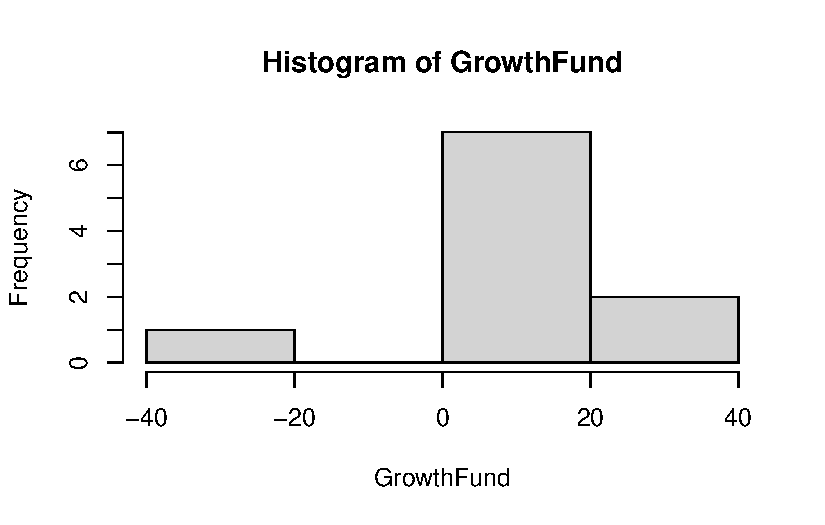
\includegraphics[keepaspectratio]{module2_files/figure-pdf/unnamed-chunk-13-1.pdf}}

\subsubsection{hist vs geom\_histogram}\label{hist-vs-geom_histogram}

\begin{itemize}
\tightlist
\item
  In R, hist() and geom\_histogram() are both used to create histograms,
  but they belong to different packages and have slightly different
  functionalities.
\end{itemize}

\begin{Shaded}
\begin{Highlighting}[]
\CommentTok{\# Making an appropriate data.frame to use the hist() command}
\NormalTok{HousePrice }\OtherTok{\textless{}{-}} \FunctionTok{c}\NormalTok{(}\DecValTok{430}\NormalTok{, }\DecValTok{520}\NormalTok{, }\DecValTok{460}\NormalTok{, }\DecValTok{475}\NormalTok{, }\DecValTok{670}\NormalTok{, }\DecValTok{521}\NormalTok{, }\DecValTok{670}\NormalTok{, }\DecValTok{417}\NormalTok{, }\DecValTok{533}\NormalTok{, }\DecValTok{525}\NormalTok{, }\DecValTok{538}\NormalTok{,}
    \DecValTok{370}\NormalTok{, }\DecValTok{530}\NormalTok{, }\DecValTok{525}\NormalTok{, }\DecValTok{430}\NormalTok{, }\DecValTok{330}\NormalTok{, }\DecValTok{575}\NormalTok{, }\DecValTok{555}\NormalTok{, }\DecValTok{521}\NormalTok{, }\DecValTok{350}\NormalTok{, }\DecValTok{399}\NormalTok{, }\DecValTok{560}\NormalTok{, }\DecValTok{440}\NormalTok{, }\DecValTok{425}\NormalTok{, }\DecValTok{669}\NormalTok{,}
    \DecValTok{660}\NormalTok{, }\DecValTok{702}\NormalTok{, }\DecValTok{540}\NormalTok{, }\DecValTok{460}\NormalTok{, }\DecValTok{588}\NormalTok{, }\DecValTok{445}\NormalTok{, }\DecValTok{412}\NormalTok{, }\DecValTok{735}\NormalTok{, }\DecValTok{537}\NormalTok{, }\DecValTok{630}\NormalTok{, }\DecValTok{430}\NormalTok{)}
\NormalTok{HousePrice }\OtherTok{\textless{}{-}} \FunctionTok{data.frame}\NormalTok{(HousePrice)}
\end{Highlighting}
\end{Shaded}

\begin{itemize}
\tightlist
\item
  hist(): This function is from the base R graphics package and is used
  to create histograms. It provides a simple way to visualize the
  distribution of a single variable.
\end{itemize}

\begin{Shaded}
\begin{Highlighting}[]
\CommentTok{\# Using base R to create the histogram.}
\FunctionTok{hist}\NormalTok{(HousePrice}\SpecialCharTok{$}\NormalTok{HousePrice, }\AttributeTok{breaks =} \DecValTok{5}\NormalTok{, }\AttributeTok{main =} \StringTok{"A Histogram"}\NormalTok{, }\AttributeTok{xlab =} \StringTok{"House Prices (in $1,000s)"}\NormalTok{,}
    \AttributeTok{col =} \StringTok{"yellow"}\NormalTok{)}
\end{Highlighting}
\end{Shaded}

\pandocbounded{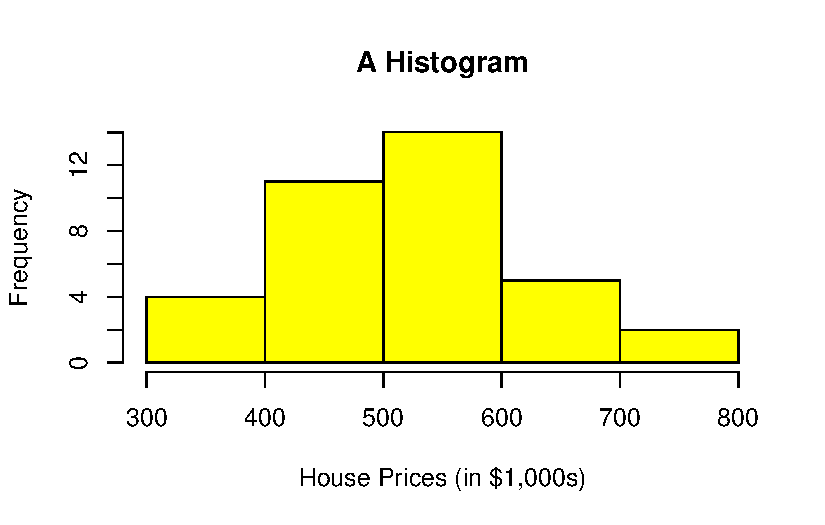
\includegraphics[keepaspectratio]{module2_files/figure-pdf/unnamed-chunk-15-1.pdf}}

\begin{Shaded}
\begin{Highlighting}[]
\FunctionTok{library}\NormalTok{(tidyverse)}
\end{Highlighting}
\end{Shaded}

\begin{itemize}
\tightlist
\item
  geom\_histogram(): This function is from the ggplot2 package, which is
  part of the tidyverse. It is used to create histograms as part of a
  more flexible and powerful plotting system.
\end{itemize}

\begin{Shaded}
\begin{Highlighting}[]
\CommentTok{\# Using geom\_histogram() command to create the histogram.}
\FunctionTok{ggplot}\NormalTok{(HousePrice, }\FunctionTok{aes}\NormalTok{(}\AttributeTok{x =}\NormalTok{ HousePrice)) }\SpecialCharTok{+} \FunctionTok{geom\_histogram}\NormalTok{(}\AttributeTok{binwidth =} \DecValTok{100}\NormalTok{,}
    \AttributeTok{boundary =} \DecValTok{300}\NormalTok{, }\AttributeTok{color =} \StringTok{"black"}\NormalTok{, }\AttributeTok{fill =} \StringTok{"yellow"}\NormalTok{) }\SpecialCharTok{+} \FunctionTok{labs}\NormalTok{(}\AttributeTok{title =} \StringTok{"A Histogram"}\NormalTok{,}
    \AttributeTok{x =} \StringTok{"House Prices (in $1,000s)"}\NormalTok{, }\AttributeTok{y =} \StringTok{"Frequency"}\NormalTok{)}
\end{Highlighting}
\end{Shaded}

\pandocbounded{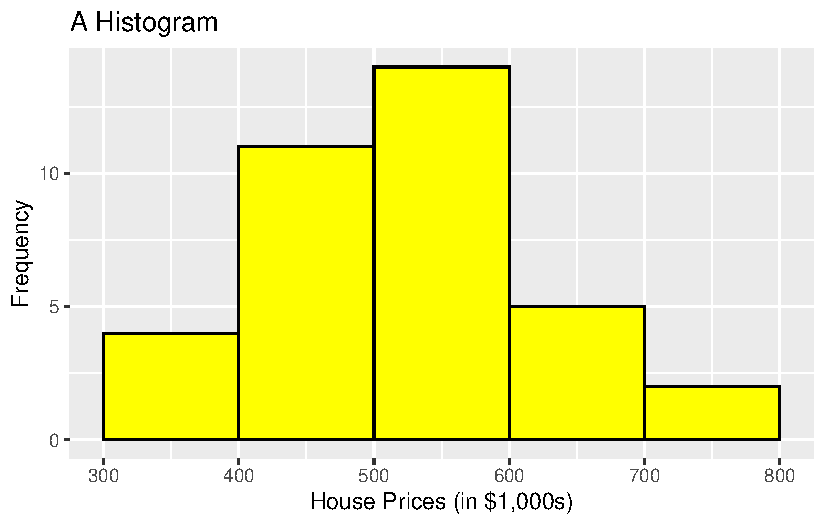
\includegraphics[keepaspectratio]{module2_files/figure-pdf/unnamed-chunk-17-1.pdf}}

\begin{itemize}
\item
  We could add more parameters here to make the 2 histograms look
  identical, but this configuration of parameters is very close. Take
  note that there are a lot more parameters you can add to the
  geom\_histogram() command than you can with base R to make it look
  more professional. Be sure to look them up and also check with the
  notes in the book, which focuses on geom\_histogram instead of hist().
\item
  Variance is a measure of spread for numeric variables that is
  essentially the average of the squared differences between each
  observation value on some variable and the mean for that variable with
  population variance.
  \[Population Var(X) = \sigma^2 = \sum{(x_i-\mu)^2}/N\]
  \[Sample Var(x) = s^2 = \sum{(x_i-\bar{x})^2}/(n-1)\]
\item
  Standard deviation is the square root of the variance.

  \begin{itemize}
  \tightlist
  \item
    Use var() command and sd() command to calculate sample variance and
    sample standard deviation.\\
  \end{itemize}

\begin{Shaded}
\begin{Highlighting}[]
\DocumentationTok{\#\# Calculated from Small Sample}
\NormalTok{x }\OtherTok{\textless{}{-}} \FunctionTok{c}\NormalTok{(}\DecValTok{1}\NormalTok{, }\DecValTok{2}\NormalTok{, }\DecValTok{3}\NormalTok{, }\DecValTok{4}\NormalTok{, }\DecValTok{5}\NormalTok{)}
\FunctionTok{sum}\NormalTok{((x }\SpecialCharTok{{-}} \FunctionTok{mean}\NormalTok{(x))}\SpecialCharTok{\^{}}\DecValTok{2}\SpecialCharTok{/}\NormalTok{(}\DecValTok{5} \SpecialCharTok{{-}} \DecValTok{1}\NormalTok{))}
\end{Highlighting}
\end{Shaded}

\begin{verbatim}
[1] 2.5
\end{verbatim}

\begin{Shaded}
\begin{Highlighting}[]
\FunctionTok{var}\NormalTok{(x)}
\end{Highlighting}
\end{Shaded}

\begin{verbatim}
[1] 2.5
\end{verbatim}

\begin{Shaded}
\begin{Highlighting}[]
\FunctionTok{sqrt}\NormalTok{(}\FunctionTok{var}\NormalTok{(x))}
\end{Highlighting}
\end{Shaded}

\begin{verbatim}
[1] 1.581139
\end{verbatim}

\begin{Shaded}
\begin{Highlighting}[]
\FunctionTok{sd}\NormalTok{(x)}
\end{Highlighting}
\end{Shaded}

\begin{verbatim}
[1] 1.581139
\end{verbatim}

\begin{Shaded}
\begin{Highlighting}[]
\FunctionTok{sd}\NormalTok{(HousePrice}\SpecialCharTok{$}\NormalTok{HousePrice)  }\CommentTok{\#102.6059}
\end{Highlighting}
\end{Shaded}

\begin{verbatim}
[1] 102.6059
\end{verbatim}

\begin{Shaded}
\begin{Highlighting}[]
\FunctionTok{var}\NormalTok{(HousePrice}\SpecialCharTok{$}\NormalTok{HousePrice)  }\CommentTok{\#10527.97}
\end{Highlighting}
\end{Shaded}

\begin{verbatim}
[1] 10527.97
\end{verbatim}

\begin{Shaded}
\begin{Highlighting}[]
\FunctionTok{skew}\NormalTok{(HousePrice}\SpecialCharTok{$}\NormalTok{HousePrice)  }\CommentTok{\#normal}
\end{Highlighting}
\end{Shaded}

\begin{verbatim}
skew (g1)        se         z         p 
    0.317     0.408     0.777     0.437 
\end{verbatim}
\item
  Looking at Spread for a Larger Dataset
\end{itemize}

\begin{Shaded}
\begin{Highlighting}[]
\NormalTok{customers }\OtherTok{\textless{}{-}} \FunctionTok{read.csv}\NormalTok{(}\StringTok{"data/customers.csv"}\NormalTok{)}
\FunctionTok{summary}\NormalTok{(customers}\SpecialCharTok{$}\NormalTok{Spending, }\AttributeTok{na.rm =} \ConstantTok{TRUE}\NormalTok{)  }\CommentTok{\#mean and median}
\end{Highlighting}
\end{Shaded}

\begin{verbatim}
   Min. 1st Qu.  Median    Mean 3rd Qu.    Max. 
   50.0   383.8   662.0   659.6   962.2  1250.0 
\end{verbatim}

\begin{Shaded}
\begin{Highlighting}[]
\FunctionTok{mean}\NormalTok{(customers}\SpecialCharTok{$}\NormalTok{Spending, }\AttributeTok{na.rm =} \ConstantTok{TRUE}\NormalTok{)  }\CommentTok{\#mean by itself}
\end{Highlighting}
\end{Shaded}

\begin{verbatim}
[1] 659.555
\end{verbatim}

\begin{Shaded}
\begin{Highlighting}[]
\FunctionTok{median}\NormalTok{(customers}\SpecialCharTok{$}\NormalTok{Spending, }\AttributeTok{na.rm =} \ConstantTok{TRUE}\NormalTok{)  }\CommentTok{\#median by itself}
\end{Highlighting}
\end{Shaded}

\begin{verbatim}
[1] 662
\end{verbatim}

\begin{Shaded}
\begin{Highlighting}[]
\DocumentationTok{\#\#\# Spread to Report with the Mean}
\FunctionTok{sd}\NormalTok{(customers}\SpecialCharTok{$}\NormalTok{Spending, }\AttributeTok{na.rm =} \ConstantTok{TRUE}\NormalTok{)}
\end{Highlighting}
\end{Shaded}

\begin{verbatim}
[1] 350.2876
\end{verbatim}

\begin{Shaded}
\begin{Highlighting}[]
\FunctionTok{var}\NormalTok{(customers}\SpecialCharTok{$}\NormalTok{Spending, }\AttributeTok{na.rm =} \ConstantTok{TRUE}\NormalTok{)}
\end{Highlighting}
\end{Shaded}

\begin{verbatim}
[1] 122701.4
\end{verbatim}

\subsubsection{Kurtosis in Evaluating Mean
Spread}\label{kurtosis-in-evaluating-mean-spread}

\begin{itemize}
\item
  Kurtosis is the sharpness of the peak of a frequency-distribution
  curve or more formally a measure of how many observations are in the
  tails of a distribution.
\item
  The formula for kurtosis is as follows: Kurtosis =
  \(\frac{n(n+1)}{(n-1)(n-2)(n-3)} \sum \left( \frac{(X_i - \bar{X})^4}{s^4} \right) - \frac{3(n-1)^2}{(n-2)(n-3)}\)
\end{itemize}

Where:

\begin{itemize}
\tightlist
\item
  \(n\) is the sample size
\item
  \(X_i\) is each individual value
\item
  \(\bar{X}\) is the mean of the data
\item
  \(s\) is the standard deviation
\item
  A normal distribution will have a kurtosis value of three, where
  distributions with kurtosis around 3 are described as mesokurtic,
  significantly higher than 3 indicate leptokurtic, and significantly
  under 3 indicate platykurtic.
\item
  The kurtosis() command from the semTools package subtracts 3 from the
  kurtosis, so we can evaluate values by comparing them to 0. Positive
  values will be indicative to a leptokurtic distribution and negative
  will indicate a platykurtic distribution. To see if kurtosis
  (leptokurtic or platykurtic) is significant, we confirm them by first
  evaluating the z-score to see if the variable is normal or not. The
  same cutoff values from skew also apply for the z for small, medium,
  and large sample sizes in kurtosis. These are the same basic rules for
  the rules in judging skewness.
\end{itemize}

\begin{figure}[H]

{\centering \pandocbounded{\includegraphics[keepaspectratio]{Pictures/Ch2/Kurtosis.png}}

}

\caption{Evaluate Kurtosis}

\end{figure}%

\begin{itemize}
\tightlist
\item
  The rules of determining problematic distributions with regards to
  kurtosis are below.

  \begin{itemize}
  \tightlist
  \item
    If the sample size is small (n \textless{} 50), z values outside the
    --2 to 2 range are a problem.
  \item
    If the sample size is between 50 and 300, z values outside the
    --3.29 to 3.29 range are a problem.
  \item
    For large samples (n \textgreater{} 300), using a visual is
    recommended over the statistics, but generally z values outside the
    range of --7 to 7 can be considered problematic.
  \item
    If kurtosis is found, then evaluate the excess kur score to see if
    it is positive or negative to determine whether it is leptokurtic or
    platykurtic.
  \end{itemize}
\end{itemize}

\begin{Shaded}
\begin{Highlighting}[]
\CommentTok{\# z{-}value is 3.0398, which is \textgreater{} 2 indicating leptokurtic Small sample}
\CommentTok{\# size: range is {-}2 to 2}
\FunctionTok{kurtosis}\NormalTok{(salaries)}
\end{Highlighting}
\end{Shaded}

\begin{verbatim}
Excess Kur (g2)              se               z               p 
          5.629           1.852           3.040           0.002 
\end{verbatim}

\begin{Shaded}
\begin{Highlighting}[]
\CommentTok{\# z{-}value is 2.20528007, which is \textgreater{} 2 indicating leptokurtic Small}
\CommentTok{\# sample size: range is {-}2 to 2}
\FunctionTok{kurtosis}\NormalTok{(GrowthFund)}
\end{Highlighting}
\end{Shaded}

\begin{verbatim}
Excess Kur (g2)              se               z               p 
          3.416           1.549           2.205           0.027 
\end{verbatim}

\begin{Shaded}
\begin{Highlighting}[]
\CommentTok{\# Small sample size: range is {-}2 to 2 Skewness and kurtosis are both}
\CommentTok{\# in range.}
\FunctionTok{skew}\NormalTok{(HousePrice}\SpecialCharTok{$}\NormalTok{HousePrice)  }\CommentTok{\#normal}
\end{Highlighting}
\end{Shaded}

\begin{verbatim}
skew (g1)        se         z         p 
    0.317     0.408     0.777     0.437 
\end{verbatim}

\begin{Shaded}
\begin{Highlighting}[]
\FunctionTok{kurtosis}\NormalTok{(HousePrice}\SpecialCharTok{$}\NormalTok{HousePrice)  }\CommentTok{\#normal}
\end{Highlighting}
\end{Shaded}

\begin{verbatim}
Excess Kur (g2)              se               z               p 
         -0.540           0.816          -0.661           0.508 
\end{verbatim}

\begin{itemize}
\tightlist
\item
  Let's do a few more examples using the customers dataset.
\end{itemize}

\begin{Shaded}
\begin{Highlighting}[]
\CommentTok{\# Noted sample size at 200 observations or a medium sample size.}
\CommentTok{\# Using threshold –3.29 to 3.29 to assess normality.}

\CommentTok{\#{-}3.4245446445 is below {-}3.29 so kurtosis is present}
\CommentTok{\# Negative kurtosis value indicates platykurtic}
\FunctionTok{kurtosis}\NormalTok{(customers}\SpecialCharTok{$}\NormalTok{Spending)}
\end{Highlighting}
\end{Shaded}

\begin{verbatim}
Excess Kur (g2)              se               z               p 
         -1.186           0.346          -3.425           0.001 
\end{verbatim}

\begin{Shaded}
\begin{Highlighting}[]
\FunctionTok{ggplot}\NormalTok{(customers, }\FunctionTok{aes}\NormalTok{(Spending)) }\SpecialCharTok{+} \FunctionTok{geom\_histogram}\NormalTok{(}\AttributeTok{binwidth =} \DecValTok{100}\NormalTok{, }\AttributeTok{fill =} \StringTok{"pink"}\NormalTok{,}
    \AttributeTok{color =} \StringTok{"black"}\NormalTok{)}
\end{Highlighting}
\end{Shaded}

\pandocbounded{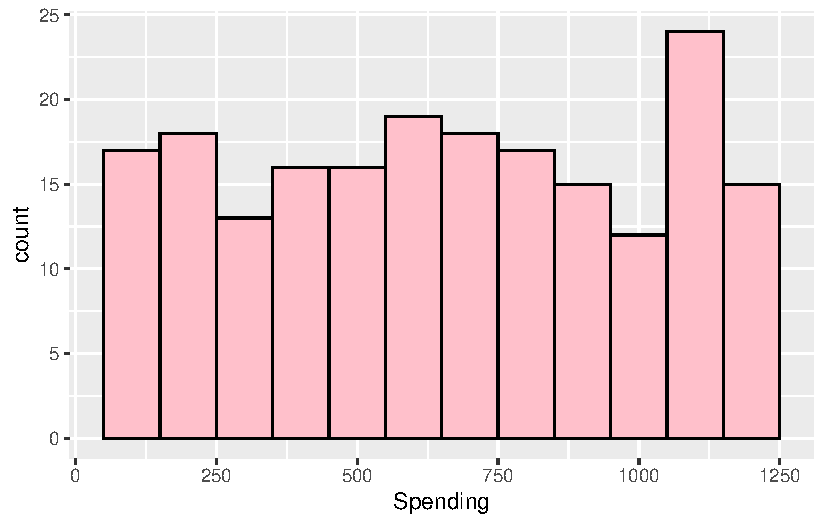
\includegraphics[keepaspectratio]{module2_files/figure-pdf/unnamed-chunk-21-1.pdf}}

\begin{Shaded}
\begin{Highlighting}[]
\NormalTok{semTools}\SpecialCharTok{::}\FunctionTok{skew}\NormalTok{(customers}\SpecialCharTok{$}\NormalTok{Spending)  }\DocumentationTok{\#\#normal indicating no skewness}
\end{Highlighting}
\end{Shaded}

\begin{verbatim}
skew (g1)        se         z         p 
   -0.018     0.173    -0.106     0.916 
\end{verbatim}

\begin{Shaded}
\begin{Highlighting}[]
\CommentTok{\# Normal: 2.977622119 is in between {-}3.29 and 3.29}
\FunctionTok{kurtosis}\NormalTok{(customers}\SpecialCharTok{$}\NormalTok{Income)}
\end{Highlighting}
\end{Shaded}

\begin{verbatim}
Excess Kur (g2)              se               z               p 
          1.031           0.346           2.978           0.003 
\end{verbatim}

\begin{Shaded}
\begin{Highlighting}[]
\FunctionTok{ggplot}\NormalTok{(customers, }\FunctionTok{aes}\NormalTok{(Income)) }\SpecialCharTok{+} \FunctionTok{geom\_histogram}\NormalTok{(}\AttributeTok{binwidth =} \DecValTok{10000}\NormalTok{, }\AttributeTok{fill =} \StringTok{"pink"}\NormalTok{,}
    \AttributeTok{color =} \StringTok{"black"}\NormalTok{)}
\end{Highlighting}
\end{Shaded}

\pandocbounded{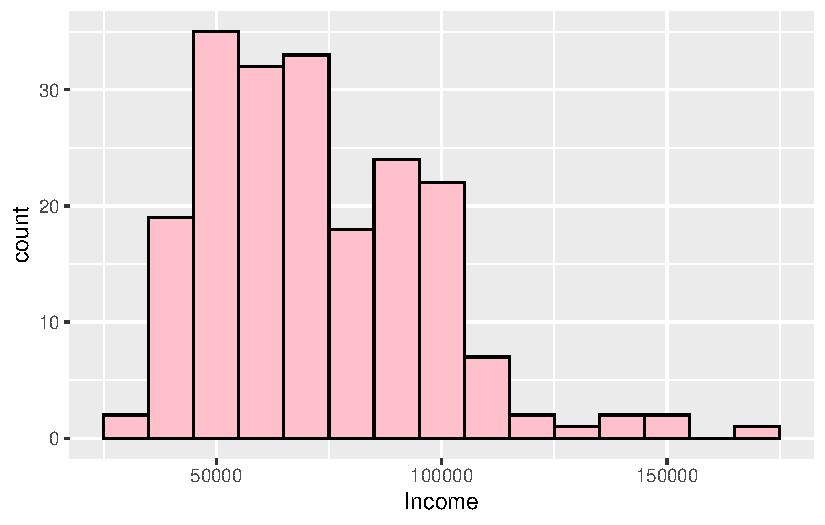
\includegraphics[keepaspectratio]{module2_files/figure-pdf/unnamed-chunk-21-2.pdf}}

\begin{Shaded}
\begin{Highlighting}[]
\NormalTok{semTools}\SpecialCharTok{::}\FunctionTok{skew}\NormalTok{(customers}\SpecialCharTok{$}\NormalTok{Income)  }\CommentTok{\#Skewed right}
\end{Highlighting}
\end{Shaded}

\begin{verbatim}
skew (g1)        se         z         p 
    0.874     0.173     5.047     0.000 
\end{verbatim}

\begin{Shaded}
\begin{Highlighting}[]
\CommentTok{\#{-}3.7251961028 is below {-}3.29 so kurtosis is present}
\CommentTok{\# Negative kurtosis value indicates platykurtic}
\FunctionTok{kurtosis}\NormalTok{(customers}\SpecialCharTok{$}\NormalTok{HHSize)}
\end{Highlighting}
\end{Shaded}

\begin{verbatim}
Excess Kur (g2)              se               z               p 
         -1.290           0.346          -3.725           0.000 
\end{verbatim}

\begin{Shaded}
\begin{Highlighting}[]
\FunctionTok{ggplot}\NormalTok{(customers, }\FunctionTok{aes}\NormalTok{(HHSize)) }\SpecialCharTok{+} \FunctionTok{geom\_histogram}\NormalTok{(}\AttributeTok{binwidth =} \DecValTok{1}\NormalTok{, }\AttributeTok{fill =} \StringTok{"pink"}\NormalTok{,}
    \AttributeTok{color =} \StringTok{"black"}\NormalTok{)}
\end{Highlighting}
\end{Shaded}

\pandocbounded{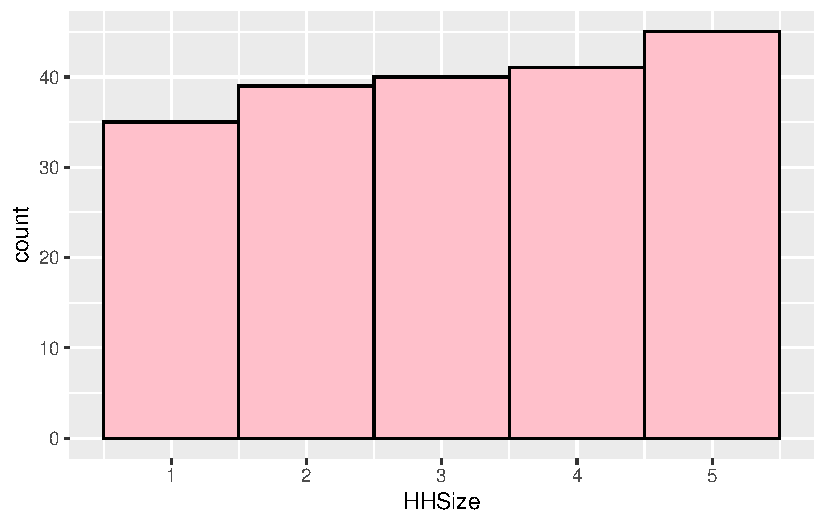
\includegraphics[keepaspectratio]{module2_files/figure-pdf/unnamed-chunk-21-3.pdf}}

\begin{Shaded}
\begin{Highlighting}[]
\NormalTok{semTools}\SpecialCharTok{::}\FunctionTok{skew}\NormalTok{(customers}\SpecialCharTok{$}\NormalTok{HHSize)  }\CommentTok{\#normal}
\end{Highlighting}
\end{Shaded}

\begin{verbatim}
skew (g1)        se         z         p 
   -0.089     0.173    -0.513     0.608 
\end{verbatim}

\begin{Shaded}
\begin{Highlighting}[]
\CommentTok{\# Normal: {-}0.20056607 is in between {-}3.29 and 3.29}
\FunctionTok{kurtosis}\NormalTok{(customers}\SpecialCharTok{$}\NormalTok{Orders)}
\end{Highlighting}
\end{Shaded}

\begin{verbatim}
Excess Kur (g2)              se               z               p 
         -0.069           0.346          -0.201           0.841 
\end{verbatim}

\begin{Shaded}
\begin{Highlighting}[]
\FunctionTok{ggplot}\NormalTok{(customers, }\FunctionTok{aes}\NormalTok{(Orders)) }\SpecialCharTok{+} \FunctionTok{geom\_histogram}\NormalTok{(}\AttributeTok{binwidth =} \DecValTok{5}\NormalTok{, }\AttributeTok{fill =} \StringTok{"pink"}\NormalTok{,}
    \AttributeTok{color =} \StringTok{"black"}\NormalTok{)}
\end{Highlighting}
\end{Shaded}

\pandocbounded{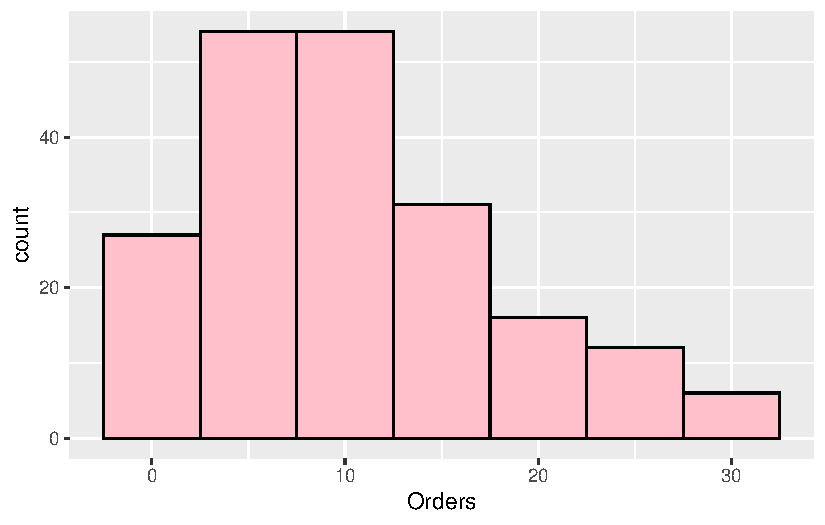
\includegraphics[keepaspectratio]{module2_files/figure-pdf/unnamed-chunk-21-4.pdf}}

\begin{Shaded}
\begin{Highlighting}[]
\NormalTok{semTools}\SpecialCharTok{::}\FunctionTok{skew}\NormalTok{(customers}\SpecialCharTok{$}\NormalTok{Orders)  }\DocumentationTok{\#\#skewed right}
\end{Highlighting}
\end{Shaded}

\begin{verbatim}
skew (g1)        se         z         p 
    0.789     0.173     4.553     0.000 
\end{verbatim}

\subsection{Spread to Report with the
Median}\label{spread-to-report-with-the-median}

\begin{itemize}
\item
  Range = Maximum Value -- Minimum Value.

  \begin{itemize}
  \tightlist
  \item
    Simplest measure.
  \item
    Focuses on Extreme values.
  \item
    Use commands diff(range()) or max() -- min().
  \end{itemize}
\item
  IQR: Difference between the first and third quartiles.

  \begin{itemize}
  \tightlist
  \item
    Use IQR() command or quantile() command.
  \end{itemize}

\begin{Shaded}
\begin{Highlighting}[]
\FunctionTok{summary}\NormalTok{(customers}\SpecialCharTok{$}\NormalTok{Spending, }\AttributeTok{na.rm =} \ConstantTok{TRUE}\NormalTok{)}
\end{Highlighting}
\end{Shaded}

\begin{verbatim}
   Min. 1st Qu.  Median    Mean 3rd Qu.    Max. 
   50.0   383.8   662.0   659.6   962.2  1250.0 
\end{verbatim}

\begin{Shaded}
\begin{Highlighting}[]
\FunctionTok{diff}\NormalTok{(}\FunctionTok{range}\NormalTok{(customers}\SpecialCharTok{$}\NormalTok{Spending, }\AttributeTok{na.rm =} \ConstantTok{TRUE}\NormalTok{))}
\end{Highlighting}
\end{Shaded}

\begin{verbatim}
[1] 1200
\end{verbatim}

\begin{Shaded}
\begin{Highlighting}[]
\FunctionTok{max}\NormalTok{(customers}\SpecialCharTok{$}\NormalTok{Spending, }\AttributeTok{na.rm =} \ConstantTok{TRUE}\NormalTok{) }\SpecialCharTok{{-}} \FunctionTok{min}\NormalTok{(customers}\SpecialCharTok{$}\NormalTok{Spending, }\AttributeTok{na.rm =} \ConstantTok{TRUE}\NormalTok{)}
\end{Highlighting}
\end{Shaded}

\begin{verbatim}
[1] 1200
\end{verbatim}

\begin{Shaded}
\begin{Highlighting}[]
\FunctionTok{IQR}\NormalTok{(customers}\SpecialCharTok{$}\NormalTok{Spending, }\AttributeTok{na.rm =} \ConstantTok{TRUE}\NormalTok{)}
\end{Highlighting}
\end{Shaded}

\begin{verbatim}
[1] 578.5
\end{verbatim}
\end{itemize}

\subsection{Spread to Report with the
Mode}\label{spread-to-report-with-the-mode}

\begin{itemize}
\tightlist
\item
  While there is no great function to test for spread, you can look at
  the data and see if it is concentrated around 1 or 2 frequencies. If
  it is, then the spread is distorted towards those high frequency
  values.
\end{itemize}

\bookmarksetup{startatroot}

\chapter{Summarizing Qualitative
Data}\label{summarizing-qualitative-data}

\begin{itemize}
\tightlist
\item
  Qualitative data is information that cannot be easily counted,
  measured, or easily expressed using numbers.

  \begin{itemize}
  \tightlist
  \item
    Nominal variables: a type of categorical variable that represents
    discrete categories or groups with no inherent order or ranking

    \begin{itemize}
    \tightlist
    \item
      gender (male, female)
    \item
      marital status (single, married, divorced)
    \item
      eye color (blue, brown, green)
    \end{itemize}
  \item
    Ordinal variables: categories possess a natural order or ranking

    \begin{itemize}
    \tightlist
    \item
      a Likert scale measuring agreement with a statement (e.g.,
      strongly disagree, disagree, neutral, agree, strongly agree)
    \end{itemize}
  \end{itemize}
\item
  A frequency distribution shows the number of observations in each
  category for a factor or categorical variable.
\item
  Guidelines when constructing frequency distribution:

  \begin{itemize}
  \tightlist
  \item
    Classes or categories are mutually exclusive (they are all unique).
  \item
    Classes or categories are exhaustive (a full list of categories).
  \end{itemize}
\item
  To calculate frequencies, first, start with a variable that has
  categorical data.
\end{itemize}

\begin{Shaded}
\begin{Highlighting}[]
\CommentTok{\# Create a vector with some data that could be categorical}
\NormalTok{Sample\_Vector }\OtherTok{\textless{}{-}} \FunctionTok{c}\NormalTok{(}\StringTok{"A"}\NormalTok{, }\StringTok{"B"}\NormalTok{, }\StringTok{"A"}\NormalTok{, }\StringTok{"C"}\NormalTok{, }\StringTok{"A"}\NormalTok{, }\StringTok{"B"}\NormalTok{, }\StringTok{"A"}\NormalTok{, }\StringTok{"C"}\NormalTok{, }\StringTok{"A"}\NormalTok{, }\StringTok{"B"}\NormalTok{)}
\CommentTok{\# Create a data frame with the vector}
\NormalTok{data }\OtherTok{\textless{}{-}} \FunctionTok{data.frame}\NormalTok{(Sample\_Vector)}
\end{Highlighting}
\end{Shaded}

\begin{itemize}
\tightlist
\item
  To count the number of each category value, we can use the table()
  command.
\item
  The output shows a top row of categories and a bottom row that
  contains the number of observations in the category.
\end{itemize}

\begin{Shaded}
\begin{Highlighting}[]
\CommentTok{\# Create a table of frequencies}
\NormalTok{frequencies }\OtherTok{\textless{}{-}} \FunctionTok{table}\NormalTok{(data}\SpecialCharTok{$}\NormalTok{Sample\_Vector)}
\NormalTok{frequencies}
\end{Highlighting}
\end{Shaded}

\begin{verbatim}

A B C 
5 3 2 
\end{verbatim}

\begin{itemize}
\tightlist
\item
  Relative frequency is how often something happens divided by all
  outcomes.
\item
  The relative frequency is calculated by \(f_i/n\), where \(f_i\) is
  the frequency of class \(i\) and \(n\) is the total frequency.
\item
  We can use the prop.table() command to calculate relative frequency by
  dividing each category's frequency by the sample size.
\end{itemize}

\begin{Shaded}
\begin{Highlighting}[]
\CommentTok{\# Calculate proportions}
\NormalTok{proportions }\OtherTok{\textless{}{-}} \FunctionTok{prop.table}\NormalTok{(frequencies)}
\end{Highlighting}
\end{Shaded}

\begin{itemize}
\tightlist
\item
  The cumulative relative frequency is given by \(cf_i/n\), where
  \(cf_i\) is the cumulative frequency of class \(i\).
\item
  The cumsum() function calculates the cumulative distribution of the
  data
\end{itemize}

\begin{Shaded}
\begin{Highlighting}[]
\CommentTok{\# Calculate cumulative frequencies}
\NormalTok{cumulfreq }\OtherTok{\textless{}{-}} \FunctionTok{cumsum}\NormalTok{(frequencies)}
\CommentTok{\# Calculate cumulative proportions}
\NormalTok{cumulproportions }\OtherTok{\textless{}{-}} \FunctionTok{cumsum}\NormalTok{(}\FunctionTok{prop.table}\NormalTok{(frequencies))}
\end{Highlighting}
\end{Shaded}

\begin{itemize}
\tightlist
\item
  The rbind() function is used to combine multiple data frames or
  matrices by row. The name ``rbind'' stands for ``row bind''. Since the
  data produced by the table is in rows, we can use rbind to link them
  together.
\end{itemize}

\begin{Shaded}
\begin{Highlighting}[]
\CommentTok{\# combine into table}
\NormalTok{frequency\_table }\OtherTok{\textless{}{-}} \FunctionTok{rbind}\NormalTok{(frequencies, proportions, cumulfreq, cumulproportions)}
\CommentTok{\# Print the table}
\NormalTok{frequency\_table}
\end{Highlighting}
\end{Shaded}

\begin{verbatim}
                   A   B    C
frequencies      5.0 3.0  2.0
proportions      0.5 0.3  0.2
cumulfreq        5.0 8.0 10.0
cumulproportions 0.5 0.8  1.0
\end{verbatim}

\begin{itemize}
\tightlist
\item
  We can transpose a table using the t() command, which flips the
  dataset.
\end{itemize}

\begin{Shaded}
\begin{Highlighting}[]
\NormalTok{TransposedData }\OtherTok{\textless{}{-}} \FunctionTok{t}\NormalTok{(frequency\_table)}
\NormalTok{TransposedData}
\end{Highlighting}
\end{Shaded}

\begin{verbatim}
  frequencies proportions cumulfreq cumulproportions
A           5         0.5         5              0.5
B           3         0.3         8              0.8
C           2         0.2        10              1.0
\end{verbatim}

\begin{itemize}
\tightlist
\item
  Finally, sometimes we need to transform our calculations into a
  dataset.
\item
  The as.data.frame function is used to coerce or convert an object into
  a data frame.
\item
  as.data.frame() is used when you have an existing object that needs to
  be coerced into a data frame. data.frame(), on the other hand, is for
  creating a data frame from scratch by specifying the data directly.
  Therefore, both as.data.frame() and data.frame() are used to convert
  or create data frames in R.
\item
  as.data.frame() coerces an existing object (such as a list, matrix, or
  vector) into a data frame. Data.frame is used to create a new data
  frame from individual vectors or lists.
\item
  as.data.frame() accepts a wider variety of inputs (like lists,
  matrices, and vectors), while data.frame() directly accepts vectors
  and lists to construct the data frame.
\end{itemize}

\begin{Shaded}
\begin{Highlighting}[]
\NormalTok{TransposedData }\OtherTok{\textless{}{-}} \FunctionTok{as.data.frame}\NormalTok{(TransposedData)}
\NormalTok{TransposedData}
\end{Highlighting}
\end{Shaded}

\begin{verbatim}
  frequencies proportions cumulfreq cumulproportions
A           5         0.5         5              0.5
B           3         0.3         8              0.8
C           2         0.2        10              1.0
\end{verbatim}

\begin{itemize}
\item
  When working with a dataset that's already provided, there's no need
  to create a new data frame in the initial steps.
\item
  The example below uses the built-in iris dataset and the Species
  variable, which is already properly coded as a categorical variable in
  R.
\item
  This example combines all the previous steps and creates a new data
  frame that includes the frequency, relative frequency, and cumulative
  values.
\end{itemize}

\begin{Shaded}
\begin{Highlighting}[]
\FunctionTok{data}\NormalTok{(}\StringTok{"iris"}\NormalTok{)}
\FunctionTok{summary}\NormalTok{(iris}\SpecialCharTok{$}\NormalTok{Species)}
\end{Highlighting}
\end{Shaded}

\begin{verbatim}
    setosa versicolor  virginica 
        50         50         50 
\end{verbatim}

\begin{Shaded}
\begin{Highlighting}[]
\NormalTok{frequencies }\OtherTok{\textless{}{-}} \FunctionTok{table}\NormalTok{(iris}\SpecialCharTok{$}\NormalTok{Species)}
\NormalTok{proportions }\OtherTok{\textless{}{-}} \FunctionTok{prop.table}\NormalTok{(frequencies)}
\NormalTok{cumulfreq }\OtherTok{\textless{}{-}} \FunctionTok{cumsum}\NormalTok{(frequencies)}
\NormalTok{cumulproportions }\OtherTok{\textless{}{-}} \FunctionTok{cumsum}\NormalTok{(}\FunctionTok{prop.table}\NormalTok{(frequencies))}
\NormalTok{frequency\_table }\OtherTok{\textless{}{-}} \FunctionTok{rbind}\NormalTok{(frequencies, proportions, cumulfreq, cumulproportions)}
\NormalTok{TransposedData }\OtherTok{\textless{}{-}} \FunctionTok{t}\NormalTok{(frequency\_table)}
\NormalTok{TransposedData }\OtherTok{\textless{}{-}} \FunctionTok{as.data.frame}\NormalTok{(TransposedData)}
\NormalTok{TransposedData}
\end{Highlighting}
\end{Shaded}

\begin{verbatim}
           frequencies proportions cumulfreq cumulproportions
setosa              50   0.3333333        50        0.3333333
versicolor          50   0.3333333       100        0.6666667
virginica           50   0.3333333       150        1.0000000
\end{verbatim}

\bookmarksetup{startatroot}

\chapter{Data Preparation}\label{data-preparation}

\begin{itemize}
\tightlist
\item
  We often spend a considerable amount of time inspecting and preparing
  the data for the subsequent analysis. This includes the following:

  \begin{itemize}
  \tightlist
  \item
    Evaluating Data Types
  \item
    Arranging Data
  \item
    Selecting Variables
  \item
    Filtering Data
  \item
    Counting Data
  \item
    Handling Missing Values
  \item
    Summarizing
  \item
    Grouping Data
  \end{itemize}
\end{itemize}

\section{Common dplyr Functions}\label{common-dplyr-functions}

\subsection{Arrange}\label{arrange}

\begin{itemize}
\tightlist
\item
  Sorting or arranging the dataset allows you to specify an order based
  on variable values.
\item
  Sorting allows us to review the range of values for each variable, and
  we can sort based on a single or multiple variables.
\item
  Notice the difference between sort() and arrange() functions below.

  \begin{itemize}
  \tightlist
  \item
    The sort() function sorts a vector.
  \item
    The arrange() function sorts a dataset based on a variable.
  \end{itemize}
\item
  To conduct an example, read in the data set called gig.csv from your
  working directory.
\end{itemize}

\begin{Shaded}
\begin{Highlighting}[]
\NormalTok{gig }\OtherTok{\textless{}{-}} \FunctionTok{read.csv}\NormalTok{(}\StringTok{"data/gig.csv"}\NormalTok{, }\AttributeTok{stringsAsFactors =} \ConstantTok{TRUE}\NormalTok{, }\AttributeTok{na.strings =} \StringTok{""}\NormalTok{)}
\FunctionTok{dim}\NormalTok{(gig)}
\end{Highlighting}
\end{Shaded}

\begin{verbatim}
[1] 604   4
\end{verbatim}

\begin{Shaded}
\begin{Highlighting}[]
\FunctionTok{head}\NormalTok{(gig)}
\end{Highlighting}
\end{Shaded}

\begin{verbatim}
  EmployeeID  Wage     Industry        Job
1          1 32.81 Construction    Analyst
2          2 46.00   Automotive   Engineer
3          3 43.13 Construction  Sales Rep
4          4 48.09   Automotive      Other
5          5 43.62   Automotive Accountant
6          6 46.98 Construction   Engineer
\end{verbatim}

\begin{itemize}
\item
  Using the arrange() function, we add the dataset, followed by a comma
  and then add in the variable we want to sort. This arranges from small
  to large.
\item
  Below is code to rearrange data based on Wage and save it in a new
  object.
\end{itemize}

\begin{Shaded}
\begin{Highlighting}[]
\NormalTok{sortTidy }\OtherTok{\textless{}{-}} \FunctionTok{arrange}\NormalTok{(gig, Wage)}
\FunctionTok{head}\NormalTok{(sortTidy)}
\end{Highlighting}
\end{Shaded}

\begin{verbatim}
  EmployeeID  Wage     Industry        Job
1        467 24.28 Construction   Engineer
2        547 24.28 Construction  Sales Rep
3        580 24.28 Construction Accountant
4        559 24.42 Construction   Engineer
5         16 24.76   Automotive Programmer
6        221 24.76   Automotive Programmer
\end{verbatim}

\begin{itemize}
\tightlist
\item
  We can apply a desc() function inside the arrange function to re-sort
  from high to low like shown below.
\end{itemize}

\begin{Shaded}
\begin{Highlighting}[]
\NormalTok{sortTidyDesc }\OtherTok{\textless{}{-}} \FunctionTok{arrange}\NormalTok{(gig, }\FunctionTok{desc}\NormalTok{(Wage))}
\FunctionTok{head}\NormalTok{(sortTidyDesc)}
\end{Highlighting}
\end{Shaded}

\begin{verbatim}
  EmployeeID  Wage     Industry        Job
1        110 51.00 Construction      Other
2         79 50.00   Automotive   Engineer
3        348 49.91 Construction Accountant
4        373 49.91 Construction Accountant
5        599 49.84   Automotive   Engineer
6         70 49.77 Construction Accountant
\end{verbatim}

\subsection{Filtering}\label{filtering}

\begin{itemize}
\item
  Filtering or subsetting a data frame is the process of indexing, or
  extracting a portion of the data set that is relevant for subsequent
  statistical analysis. Subsetting allows you to work with a subset of
  your data, which is essential for data analysis and manipulation. One
  of the most common ways to subset in R is by using square brackets
  {[}{]}. We can also use the filter() function from tidyverse.
\item
  We use subsets to do the following:

  \begin{itemize}
  \tightlist
  \item
    View data based on specific data values or ranges.
  \item
    Compare two or more subsets of the data.
  \item
    Eliminate observations that contain missing values, low-quality
    data, or outliers.
  \item
    Exclude variables that contain redundant information, or variables
    with excessive amounts of missing values.
  \end{itemize}
\item
  When working with data frames, you can subset by rows and columns
  using two indices inside the square brackets: data{[}row, column{]}.
  For example, if you have df \textless- data.frame(a = 1:3, b =
  c(``X'', ``Y'', ``Z'')), df{[}1, 2{]} would return the value ``X'',
  which is the first row and second column. If you want the entire first
  row, you would use df{[}1, {]}, and to get the second column, you'd
  use df{[}, 2{]}.
\item
  You can also use logical conditions to subset. For instance, x{[}x
  \textgreater{} 20{]} would return all values in x greater than 20, and
  in a data frame, you could filter rows where a certain condition
  holds, such as df{[}df\$a \textgreater{} 1, {]}, which returns rows
  where column a has values greater than 1.
\item
  Let's do an example using the customers.csv file we read in earlier as
  customers in the last lesson. Base R provides several methods for
  subsetting data structures. Below uses base R by using the square
  brackets dataset{[}row, column{]} format.
\end{itemize}

\begin{Shaded}
\begin{Highlighting}[]
\NormalTok{customers }\OtherTok{\textless{}{-}} \FunctionTok{read.csv}\NormalTok{(}\StringTok{"data/customers.csv"}\NormalTok{, }\AttributeTok{stringsAsFactors =} \ConstantTok{TRUE}\NormalTok{)}

\CommentTok{\# To subset, note the dataset[row,column] format Results hidden to}
\CommentTok{\# save space, but be sure to try this code in your .R file.  Data in}
\CommentTok{\# 1st row}
\NormalTok{customers[}\DecValTok{1}\NormalTok{, ]}
\CommentTok{\# Data in 2nd column}
\NormalTok{customers[, }\DecValTok{2}\NormalTok{]}
\CommentTok{\# Data for 2nd column/1st observation (row)}
\NormalTok{customers[}\DecValTok{1}\NormalTok{, }\DecValTok{2}\NormalTok{]}
\CommentTok{\# First 3 columns of data}
\NormalTok{customers[, }\DecValTok{1}\SpecialCharTok{:}\DecValTok{3}\NormalTok{]}
\end{Highlighting}
\end{Shaded}

\begin{itemize}
\tightlist
\item
  One of the most powerful and intuitive ways to subset data frames in R
  is by using the filter() function from the dplyr package, which is
  part of the tidyverse. Tidyverse is extremely popular when filtering
  data.
\item
  The filter function is used to subset rows of a data frame based on
  certain conditions.
\item
  The below example filters data by the College variable when category
  values are ``Yes'' and saves the filtered dataset into an object
  called college.
\end{itemize}

\begin{Shaded}
\begin{Highlighting}[]
\CommentTok{\# Filtering by whether the customer has a \textquotesingle{}Yes\textquotesingle{} for college.  Saving}
\CommentTok{\# this filter into a new object college which you should see in your}
\CommentTok{\# global environment.}
\NormalTok{college }\OtherTok{\textless{}{-}} \FunctionTok{filter}\NormalTok{(customers, College }\SpecialCharTok{==} \StringTok{"Yes"}\NormalTok{)}
\CommentTok{\# Showing first 6 records of college {-} note the College variable is}
\CommentTok{\# all Yes\textquotesingle{}s.}
\FunctionTok{head}\NormalTok{(college)}
\end{Highlighting}
\end{Shaded}

\begin{verbatim}
   CustID    Sex     Race  BirthDate College HHSize Income Spending Orders
1 1530016 Female    Black 12/16/1986     Yes      5  53000      241      3
2 1531136   Male    White   5/9/1993     Yes      5  94000      843     12
3 1532160   Male    Black  5/22/1966     Yes      2  64000      719      9
4 1532307   Male    White  9/16/1964     Yes      4  60000      582     13
5 1532387   Male    White  8/27/1957     Yes      2  67000      452      9
6 1533017 Female Hispanic  5/14/1985     Yes      3  84000      153      2
  Channel
1      SM
2      TV
3      TV
4      SM
5      SM
6     Web
\end{verbatim}

\begin{itemize}
\tightlist
\item
  Using the filter command, we can add filters pretty easily by using an
  \& for and, or an \textbar{} for or. The statement below filters by
  College \emph{and} Income and save the new dataset in an object called
  twoFilters.
\end{itemize}

\begin{Shaded}
\begin{Highlighting}[]
\NormalTok{twoFilters }\OtherTok{\textless{}{-}} \FunctionTok{filter}\NormalTok{(customers, College }\SpecialCharTok{==} \StringTok{"Yes"} \SpecialCharTok{\&}\NormalTok{ Income }\SpecialCharTok{\textless{}} \DecValTok{50000}\NormalTok{)}
\FunctionTok{head}\NormalTok{(twoFilters)}
\end{Highlighting}
\end{Shaded}

\begin{verbatim}
   CustID    Sex     Race  BirthDate College HHSize Income Spending Orders
1 1533697 Female    Asian  10/8/1974     Yes      3  42000      247      3
2 1535063 Female    White 12/17/1982     Yes      3  42000      313      4
3 1544417   Male Hispanic  3/14/1980     Yes      4  46000      369      3
4 1547864 Female Hispanic  6/15/1987     Yes      2  44000      500      5
5 1550969 Female    White   4/8/1978     Yes      4  47000      774     16
6 1553660 Female    White   8/2/1988     Yes      2  47000      745      5
  Channel
1     Web
2      TV
3      TV
4      TV
5      TV
6      SM
\end{verbatim}

\begin{itemize}
\tightlist
\item
  Next, we can do an \emph{or} statement. The example below uses the
  filter command to filter by more than one category in the same field
  using the \textbar{} in between the categories.
\end{itemize}

\begin{Shaded}
\begin{Highlighting}[]
\NormalTok{TwoRaces }\OtherTok{\textless{}{-}} \FunctionTok{filter}\NormalTok{(customers, Race }\SpecialCharTok{==} \StringTok{"Black"} \SpecialCharTok{|}\NormalTok{ Race }\SpecialCharTok{==} \StringTok{"White"}\NormalTok{)}
\FunctionTok{head}\NormalTok{(TwoRaces)}
\end{Highlighting}
\end{Shaded}

\begin{verbatim}
   CustID    Sex  Race  BirthDate College HHSize Income Spending Orders Channel
1 1530016 Female Black 12/16/1986     Yes      5  53000      241      3      SM
2 1531136   Male White   5/9/1993     Yes      5  94000      843     12      TV
3 1532160   Male Black  5/22/1966     Yes      2  64000      719      9      TV
4 1532307   Male White  9/16/1964     Yes      4  60000      582     13      SM
5 1532387   Male White  8/27/1957     Yes      2  67000      452      9      SM
6 1533791   Male White 10/27/1999     Yes      1  97000     1028     17     Web
\end{verbatim}

\begin{itemize}
\tightlist
\item
  The str\_detect() function is used to detect the presence or absence
  of a pattern (regular expression) in a string or vector of strings. It
  returns a logical vector indicating whether the pattern was found in
  each element of the input vector.
\item
  Using str\_detect it with a filter function allows you to pull
  observations based on the inclusion of a string pattern.
\end{itemize}

\begin{Shaded}
\begin{Highlighting}[]
\FunctionTok{library}\NormalTok{(tidyverse)}
\NormalTok{Birthday2000 }\OtherTok{\textless{}{-}} \FunctionTok{filter}\NormalTok{(customers, }\FunctionTok{str\_detect}\NormalTok{(BirthDate, }\StringTok{"1985"}\NormalTok{))}
\end{Highlighting}
\end{Shaded}

\subsection{Select}\label{select}

\begin{itemize}
\tightlist
\item
  In R, the select() function is part of the dplyr package, which is
  used for data manipulation. The select() function is specifically
  designed to subset or choose specific columns from a data frame. It
  allows you to select variables (columns) by their names or indices.
\item
  Both statements below select Income, Spending, and Orders variables
  from the customers dataset and form them into a new dataset called
  smallData.
\item
  The statements are written with and without the chaining operator.
\end{itemize}

\begin{Shaded}
\begin{Highlighting}[]
\NormalTok{smallData }\OtherTok{\textless{}{-}} \FunctionTok{select}\NormalTok{(customers, Income, Spending, Orders)}
\FunctionTok{head}\NormalTok{(smallData)}
\end{Highlighting}
\end{Shaded}

\begin{verbatim}
  Income Spending Orders
1  53000      241      3
2  94000      843     12
3  64000      719      9
4  60000      582     13
5  47000      845      7
6  67000      452      9
\end{verbatim}

\subsection{Piping (Chaining) Operator}\label{piping-chaining-operator}

\begin{itemize}
\tightlist
\item
  The pipe operator takes the output of the expression on its left-hand
  side and passes it as the first argument to the function on its
  right-hand side. This enables you to chain multiple functions
  together, making the code easier to understand and debug.
\item
  If we want to keep our code tidy, we can add the piping operator
  (\%\textgreater\%) to help combine our lines of code into a new object
  or overwriting the same object.
\item
  This operator allows us to pass the result of one function/argument to
  the other one in sequence.
\item
  The below example uses a select function to pull Income, Spending, and
  Orders variables from the customers dataset and save it as a new
  object called smallData. It is an identical request to the one
  directly above, but written with the piping operator.
\end{itemize}

\begin{Shaded}
\begin{Highlighting}[]
\NormalTok{smallData }\OtherTok{\textless{}{-}}\NormalTok{ customers }\SpecialCharTok{\%\textgreater{}\%}
    \FunctionTok{select}\NormalTok{(Income, Spending, Orders)}
\end{Highlighting}
\end{Shaded}

\subsection{Counting}\label{counting}

\begin{itemize}
\item
  Counting allows us to gain a better understanding and insights into
  the data.
\item
  This helps to verify that the data set is complete or determine if
  there are missing values.
\item
  In R, the length() function returns the number of elements in a
  vector, list, or any other object with a length attribute. It
  essentially counts the number of elements in the specified object.
\end{itemize}

\begin{Shaded}
\begin{Highlighting}[]
\CommentTok{\# Gives the length of Industry}
\FunctionTok{length}\NormalTok{(gig}\SpecialCharTok{$}\NormalTok{Industry)}
\end{Highlighting}
\end{Shaded}

\begin{verbatim}
[1] 604
\end{verbatim}

\begin{itemize}
\tightlist
\item
  For counting using tidyverse, we typically use the filter and count
  function together to filter by a value or state and then count the
  filtered data.
\item
  In the function below, I use the piping operator to link together the
  filter and count functions into one command.
\item
  Note that we need a piping operator (\%\textgreater\%) before each new
  function that is part of the chunk.
\end{itemize}

\begin{Shaded}
\begin{Highlighting}[]
\CommentTok{\# Counting with a Categorical Variable Here we are filtering by}
\CommentTok{\# Automotive Industry and then counting the number and saving it in a}
\CommentTok{\# new object called countAuto}
\NormalTok{countAuto }\OtherTok{\textless{}{-}}\NormalTok{ gig }\SpecialCharTok{\%\textgreater{}\%}
    \FunctionTok{filter}\NormalTok{(Industry }\SpecialCharTok{==} \StringTok{"Automotive"}\NormalTok{) }\SpecialCharTok{\%\textgreater{}\%}
    \FunctionTok{count}\NormalTok{()}
\NormalTok{countAuto  }\CommentTok{\#190}
\end{Highlighting}
\end{Shaded}

\begin{verbatim}
    n
1 190
\end{verbatim}

\begin{itemize}
\tightlist
\item
  Below, we are filtering by Wage and the counting.
\end{itemize}

\begin{Shaded}
\begin{Highlighting}[]
\CommentTok{\# Counting with a Numerical Variable We could also save this in an}
\CommentTok{\# object.}
\NormalTok{gig }\SpecialCharTok{\%\textgreater{}\%}
    \FunctionTok{filter}\NormalTok{(Wage }\SpecialCharTok{\textgreater{}} \DecValTok{30}\NormalTok{) }\SpecialCharTok{\%\textgreater{}\%}
    \FunctionTok{count}\NormalTok{()  }\DocumentationTok{\#\#536}
\end{Highlighting}
\end{Shaded}

\begin{verbatim}
    n
1 536
\end{verbatim}

\begin{itemize}
\item
  We learned that there are 190 employees in the automotive industry and
  there are 536 employees who earn more than \$30 per hour.
\item
  We could also calculate the number of people with wages under or equal
  to 30.
\end{itemize}

\begin{Shaded}
\begin{Highlighting}[]
\CommentTok{\# We find 68 Wages under or equal to 30}
\NormalTok{WageLess30 }\OtherTok{\textless{}{-}}\NormalTok{ gig }\SpecialCharTok{\%\textgreater{}\%}
    \FunctionTok{filter}\NormalTok{(Wage }\SpecialCharTok{\textless{}=} \DecValTok{30}\NormalTok{) }\SpecialCharTok{\%\textgreater{}\%}
    \FunctionTok{count}\NormalTok{()  }\CommentTok{\#}
\NormalTok{WageLess30}
\end{Highlighting}
\end{Shaded}

\begin{verbatim}
   n
1 68
\end{verbatim}

\begin{itemize}
\tightlist
\item
  How many Accountants are there in the Job Category of the gig data
  set. The answer is shown below. Use filter and count to calculate this
  answer.
\end{itemize}

\begin{verbatim}
   n
1 83
\end{verbatim}

\subsection{Summarize}\label{summarize}

\begin{itemize}
\tightlist
\item
  The summarize() command is used to create summary statistics for
  groups of observations in a data frame.
\item
  In R, summary() and summarize() serve different purposes. summary() is
  part of base R and gives a quick overview of data, returning
  descriptive statistics for each column. For example, summary(mtcars)
  provides the min, max, median, and mean for numeric columns and counts
  for factors. It's useful for a broad snapshot of your dataset.
\item
  In contrast, summarize() (or summarise()) is from the dplyr package
  and allows for custom summaries. For instance, mtcars \%\textgreater\%
  summarize(avg\_mpg = mean(mpg), max\_hp = max(hp)) returns the average
  miles per gallon and the maximum horsepower. It's more flexible and is
  often used with group\_by() for grouped calculations. In conclusion,
  summary() gives automatic overviews, while summarize() is better for
  tailored summaries.
\item
  In the example below, we can summarize more than one thing into tidy
  output.
\end{itemize}

\begin{Shaded}
\begin{Highlighting}[]
\NormalTok{gig }\SpecialCharTok{\%\textgreater{}\%}
    \FunctionTok{drop\_na}\NormalTok{() }\SpecialCharTok{\%\textgreater{}\%}
    \FunctionTok{summarize}\NormalTok{(}\AttributeTok{mean.days =} \FunctionTok{mean}\NormalTok{(Wage), }\AttributeTok{sd.days =} \FunctionTok{sd}\NormalTok{(Wage), }\AttributeTok{var.days =} \FunctionTok{var}\NormalTok{(Wage),}
        \AttributeTok{med.days =} \FunctionTok{median}\NormalTok{(Wage), }\AttributeTok{iqr.days =} \FunctionTok{IQR}\NormalTok{(Wage))}
\end{Highlighting}
\end{Shaded}

\begin{verbatim}
  mean.days  sd.days var.days med.days iqr.days
1  40.14567 7.047058 49.66103    41.82   11.465
\end{verbatim}

\subsection{Group\_by}\label{group_by}

\begin{itemize}
\tightlist
\item
  group\_by is used for grouping data by one or more variables. When you
  use group\_by() on a data frame, it doesn't actually perform any
  computations immediately. Instead, it sets up the data frame in such a
  way that any subsequent operations are performed within these groups
\item
  summarize() is often used in combination with group\_by() to calculate
  summary statistics within groups
\end{itemize}

\begin{Shaded}
\begin{Highlighting}[]
\DocumentationTok{\#\# summarize data by Industry variable.}
\NormalTok{groupedData }\OtherTok{\textless{}{-}}\NormalTok{ gig }\SpecialCharTok{\%\textgreater{}\%}
    \FunctionTok{group\_by}\NormalTok{(Industry) }\SpecialCharTok{\%\textgreater{}\%}
    \FunctionTok{summarize}\NormalTok{(}\AttributeTok{meanWage =} \FunctionTok{mean}\NormalTok{(Wage))}
\NormalTok{groupedData}
\end{Highlighting}
\end{Shaded}

\begin{verbatim}
# A tibble: 4 x 2
  Industry     meanWage
  <fct>           <dbl>
1 Automotive       43.4
2 Construction     38.3
3 Tech             40.7
4 <NA>             39.5
\end{verbatim}

\begin{Shaded}
\begin{Highlighting}[]
\DocumentationTok{\#\# same function with na\textquotesingle{}s dropped.}
\NormalTok{groupedData }\OtherTok{\textless{}{-}}\NormalTok{ gig }\SpecialCharTok{\%\textgreater{}\%}
    \FunctionTok{drop\_na}\NormalTok{() }\SpecialCharTok{\%\textgreater{}\%}
    \FunctionTok{group\_by}\NormalTok{(Industry) }\SpecialCharTok{\%\textgreater{}\%}
    \FunctionTok{summarize}\NormalTok{(}\AttributeTok{meanWage =} \FunctionTok{mean}\NormalTok{(Wage))}
\NormalTok{groupedData}
\end{Highlighting}
\end{Shaded}

\begin{verbatim}
# A tibble: 3 x 2
  Industry     meanWage
  <fct>           <dbl>
1 Automotive       43.4
2 Construction     38.4
3 Tech             40.7
\end{verbatim}

\subsection{Mutate}\label{mutate}

\begin{itemize}
\tightlist
\item
  mutate() is part of the dplyr package, which is used for data
  manipulation. The mutate() function is specifically designed to create
  new variables (columns) or modify existing variables in a data frame.
  It is commonly used in data wrangling tasks to add calculated columns
  or transform existing ones.
\item
  One example is below, but note that there are many things you can do
  with the mutate function.
\end{itemize}

\begin{Shaded}
\begin{Highlighting}[]
\FunctionTok{library}\NormalTok{(Amelia)}
\FunctionTok{data}\NormalTok{(}\StringTok{"africa"}\NormalTok{)}

\CommentTok{\# making a new variable called calculation that multiplies gdp\_pc by}
\CommentTok{\# infl variables in the africa1 dataset.}
\NormalTok{africa.mutated }\OtherTok{\textless{}{-}} \FunctionTok{mutate}\NormalTok{(africa, }\AttributeTok{calculation =}\NormalTok{ gdp\_pc }\SpecialCharTok{*}\NormalTok{ infl)}
\FunctionTok{head}\NormalTok{(africa.mutated)}
\end{Highlighting}
\end{Shaded}

\begin{verbatim}
  year      country gdp_pc  infl trade    civlib population calculation
1 1972 Burkina Faso    377 -2.92 29.69 0.5000000    5848380    -1100.84
2 1973 Burkina Faso    376  7.60 31.31 0.5000000    5958700     2857.60
3 1974 Burkina Faso    393  8.72 35.22 0.3333333    6075700     3426.96
4 1975 Burkina Faso    416 18.76 40.11 0.3333333    6202000     7804.16
5 1976 Burkina Faso    435 -8.40 37.76 0.5000000    6341030    -3654.00
6 1977 Burkina Faso    448 29.99 41.11 0.6666667    6486870    13435.52
\end{verbatim}

\begin{itemize}
\tightlist
\item
  Below is an example with the iris dataset, which is part of base R.
\end{itemize}

\begin{Shaded}
\begin{Highlighting}[]
\FunctionTok{data}\NormalTok{(}\StringTok{"iris"}\NormalTok{)}
\DocumentationTok{\#\# Selecting 2 variables from the iris dataset: Sepal.Length and}
\DocumentationTok{\#\# Petal.Length}
\NormalTok{selected\_data }\OtherTok{\textless{}{-}} \FunctionTok{select}\NormalTok{(iris, Sepal.Length, Petal.Length)}
\FunctionTok{head}\NormalTok{(selected\_data)}
\end{Highlighting}
\end{Shaded}

\begin{verbatim}
  Sepal.Length Petal.Length
1          5.1          1.4
2          4.9          1.4
3          4.7          1.3
4          4.6          1.5
5          5.0          1.4
6          5.4          1.7
\end{verbatim}

\begin{Shaded}
\begin{Highlighting}[]
\CommentTok{\# Filter rows based on a condition: Species = setosa}
\NormalTok{filtered\_data }\OtherTok{\textless{}{-}} \FunctionTok{filter}\NormalTok{(iris, Species }\SpecialCharTok{==} \StringTok{"setosa"}\NormalTok{)}
\FunctionTok{head}\NormalTok{(filtered\_data)}
\end{Highlighting}
\end{Shaded}

\begin{verbatim}
  Sepal.Length Sepal.Width Petal.Length Petal.Width Species
1          5.1         3.5          1.4         0.2  setosa
2          4.9         3.0          1.4         0.2  setosa
3          4.7         3.2          1.3         0.2  setosa
4          4.6         3.1          1.5         0.2  setosa
5          5.0         3.6          1.4         0.2  setosa
6          5.4         3.9          1.7         0.4  setosa
\end{verbatim}

\begin{Shaded}
\begin{Highlighting}[]
\CommentTok{\# Arrange rows by the Sepal.Length column}
\NormalTok{arranged\_data }\OtherTok{\textless{}{-}} \FunctionTok{arrange}\NormalTok{(iris, Sepal.Length)}
\CommentTok{\# Create a new column by mutating the data by transforming}
\CommentTok{\# Petal.Width to the log form.}
\NormalTok{mutated\_data }\OtherTok{\textless{}{-}} \FunctionTok{mutate}\NormalTok{(iris, }\AttributeTok{Petal.Width\_Log =} \FunctionTok{log}\NormalTok{(Petal.Width))}
\end{Highlighting}
\end{Shaded}

\section{Full Examples}\label{full-examples}

\subsection{gss.2016 Data Cleaning}\label{gss.2016-data-cleaning}

\begin{itemize}
\tightlist
\item
  First, because we made some edits to the data set, reread in version a
  using the read.csv command. This brings the data set back to its
  original form. It is always a good idea to read the dataset back in
  when you are unsure about whether you have made a mistake during data
  preparation that could cause a lack of data integrity.\\
\end{itemize}

\begin{Shaded}
\begin{Highlighting}[]
\NormalTok{gss}\FloatTok{.2016} \OtherTok{\textless{}{-}} \FunctionTok{read.csv}\NormalTok{(}\AttributeTok{file =} \StringTok{"data/gss2016.csv"}\NormalTok{)}
\end{Highlighting}
\end{Shaded}

\begin{itemize}
\tightlist
\item
  Before we remove any missing data, we need it to be the correct data
  type. In this case, grass should be a factor.
\end{itemize}

\begin{Shaded}
\begin{Highlighting}[]
\CommentTok{\# We coerced this variable earlier, but the object was called}
\CommentTok{\# gss.2016.  Since we reread in the data set, this needs to be done}
\CommentTok{\# again.}
\NormalTok{gss}\FloatTok{.2016}\SpecialCharTok{$}\NormalTok{grass }\OtherTok{\textless{}{-}} \FunctionTok{as.factor}\NormalTok{(gss}\FloatTok{.2016}\SpecialCharTok{$}\NormalTok{grass)}
\end{Highlighting}
\end{Shaded}

\begin{itemize}
\tightlist
\item
  The statement below is an equivalent to the function above, but
  written with the piping operator. It is overwriting gss.2016 after
  conducting the coercion to factor.
\item
  We added the mutate function because we are going to add other data
  cleaning tasks to this statement.
\end{itemize}

\begin{Shaded}
\begin{Highlighting}[]
\NormalTok{gss}\FloatTok{.2016} \OtherTok{\textless{}{-}}\NormalTok{ gss}\FloatTok{.2016} \SpecialCharTok{\%\textgreater{}\%}
    \FunctionTok{mutate}\NormalTok{(}\AttributeTok{grass =} \FunctionTok{as.factor}\NormalTok{(grass))}
\end{Highlighting}
\end{Shaded}

\subsubsection{Piping to More Functions: Missing
Data}\label{piping-to-more-functions-missing-data}

\begin{itemize}
\tightlist
\item
  In the code below, the as.factor() command has been moved inside a
  broader mutate statement (that uses tidyverse library) and piped to it
  the na\_if() command that handles missing data. If you use more than
  one data manipulation statement, the mutate() command is needed to
  help organize your code with one mutate() is needed for each major
  change you are making.
\item
  In the code below, we created a new object gss.2016.cleaned to help
  store the cleaned version of the dataset. This helps maintain data
  integrity because your original dataset is still intact and each time,
  you rerun the entire chunk, which includes all the changes at one
  time.
\end{itemize}

\begin{Shaded}
\begin{Highlighting}[]
\NormalTok{gss.}\FloatTok{2016.}\NormalTok{cleaned }\OtherTok{\textless{}{-}}\NormalTok{ gss}\FloatTok{.2016} \SpecialCharTok{\%\textgreater{}\%}
    \CommentTok{\# Moved coercion statement into a mutate function to keep code}
    \CommentTok{\# tidy}
\FunctionTok{mutate}\NormalTok{(}\AttributeTok{grass =} \FunctionTok{as.factor}\NormalTok{(grass)) }\SpecialCharTok{\%\textgreater{}\%}
    \CommentTok{\# Moving DK value to NA for not applicable}
\FunctionTok{mutate}\NormalTok{(}\AttributeTok{grass =} \FunctionTok{na\_if}\NormalTok{(}\AttributeTok{x =}\NormalTok{ grass, }\AttributeTok{y =} \StringTok{"DK"}\NormalTok{))}

\CommentTok{\# Check the summary, there should be 110 + 3 = 113 in the NA category}
\FunctionTok{summary}\NormalTok{(}\AttributeTok{object =}\NormalTok{ gss.}\FloatTok{2016.}\NormalTok{cleaned)}
\end{Highlighting}
\end{Shaded}

\begin{verbatim}
       grass          age           
 DK       :   0   Length:2867       
 IAP      : 911   Class :character  
 LEGAL    :1126   Mode  :character  
 NOT LEGAL: 717                     
 NA's     : 113                     
\end{verbatim}

\subsubsection{Drop Levels}\label{drop-levels}

\begin{itemize}
\item
  The droplevels function is part of base R and is used to drop unused
  levels from factor variables in a data frame. It works by removing any
  levels from a factor variable that are not present in the data.
\item
  Next, we want to edit our code to convert IAP and DK to NA values and
  drop levels that have are empty.

  \begin{itemize}
  \tightlist
  \item
    Note the Piping operator added to the end of the DK line so you can
    keep going with new commands editing gss.2016.cleaned.
  \end{itemize}

\begin{Shaded}
\begin{Highlighting}[]
\NormalTok{gss.}\FloatTok{2016.}\NormalTok{cleaned }\OtherTok{\textless{}{-}}\NormalTok{ gss}\FloatTok{.2016} \SpecialCharTok{\%\textgreater{}\%}
    \FunctionTok{mutate}\NormalTok{(}\AttributeTok{grass =} \FunctionTok{as.factor}\NormalTok{(grass)) }\SpecialCharTok{\%\textgreater{}\%}
    \CommentTok{\# Added piping operator}
\FunctionTok{mutate}\NormalTok{(}\AttributeTok{grass =} \FunctionTok{na\_if}\NormalTok{(}\AttributeTok{x =}\NormalTok{ grass, }\AttributeTok{y =} \StringTok{"DK"}\NormalTok{)) }\SpecialCharTok{\%\textgreater{}\%}
    \CommentTok{\# Turn to na if value of grass = IAP}
\FunctionTok{mutate}\NormalTok{(}\AttributeTok{grass =} \FunctionTok{na\_if}\NormalTok{(}\AttributeTok{x =}\NormalTok{ grass, }\AttributeTok{y =} \StringTok{"IAP"}\NormalTok{)) }\SpecialCharTok{\%\textgreater{}\%}
    \CommentTok{\# Drop levels in grass that have no values}
\FunctionTok{mutate}\NormalTok{(}\AttributeTok{grass =} \FunctionTok{droplevels}\NormalTok{(}\AttributeTok{x =}\NormalTok{ grass))}
\CommentTok{\# Check what you just did}
\FunctionTok{summary}\NormalTok{(gss.}\FloatTok{2016.}\NormalTok{cleaned)}
\end{Highlighting}
\end{Shaded}

\begin{verbatim}
       grass          age           
 LEGAL    :1126   Length:2867       
 NOT LEGAL: 717   Class :character  
 NA's     :1024   Mode  :character  
\end{verbatim}
\end{itemize}

\subsubsection{Coercing to Numeric}\label{coercing-to-numeric}

\begin{itemize}
\tightlist
\item
  Next, we handle a numerical variable, age. Age again has an issue
  being able to be numerical data type because it has ``89 OR OLDER'' as
  a value. Before using the as.numeric() command, we need to recode it.
  We did this above as a stand-alone statement.\\
\end{itemize}

\begin{Shaded}
\begin{Highlighting}[]
\NormalTok{gss.}\FloatTok{2016.}\NormalTok{cleaned }\OtherTok{\textless{}{-}}\NormalTok{ gss}\FloatTok{.2016} \SpecialCharTok{\%\textgreater{}\%}
    \FunctionTok{mutate}\NormalTok{(}\AttributeTok{grass =} \FunctionTok{as.factor}\NormalTok{(grass)) }\SpecialCharTok{\%\textgreater{}\%}
    \FunctionTok{mutate}\NormalTok{(}\AttributeTok{grass =} \FunctionTok{na\_if}\NormalTok{(}\AttributeTok{x =}\NormalTok{ grass, }\AttributeTok{y =} \StringTok{"DK"}\NormalTok{)) }\SpecialCharTok{\%\textgreater{}\%}
    \FunctionTok{mutate}\NormalTok{(}\AttributeTok{grass =} \FunctionTok{na\_if}\NormalTok{(}\AttributeTok{x =}\NormalTok{ grass, }\AttributeTok{y =} \StringTok{"IAP"}\NormalTok{)) }\SpecialCharTok{\%\textgreater{}\%}
    \CommentTok{\# Added piping operator}
\FunctionTok{mutate}\NormalTok{(}\AttributeTok{grass =} \FunctionTok{droplevels}\NormalTok{(}\AttributeTok{x =}\NormalTok{ grass)) }\SpecialCharTok{\%\textgreater{}\%}
    \CommentTok{\# Ensure variable can be coded as numeric and fix if necessary.}
\FunctionTok{mutate}\NormalTok{(}\AttributeTok{age =} \FunctionTok{recode}\NormalTok{(age, }\StringTok{\textasciigrave{}}\AttributeTok{89 OR OLDER}\StringTok{\textasciigrave{}} \OtherTok{=} \StringTok{"89"}\NormalTok{)) }\SpecialCharTok{\%\textgreater{}\%}
    \CommentTok{\# Coerce into numeric}
\FunctionTok{mutate}\NormalTok{(}\AttributeTok{age =} \FunctionTok{as.numeric}\NormalTok{(}\AttributeTok{x =}\NormalTok{ age))}

\CommentTok{\# Check what you just did}
\FunctionTok{summary}\NormalTok{(gss.}\FloatTok{2016.}\NormalTok{cleaned)}
\end{Highlighting}
\end{Shaded}

\begin{verbatim}
       grass           age       
 LEGAL    :1126   Min.   :18.00  
 NOT LEGAL: 717   1st Qu.:34.00  
 NA's     :1024   Median :49.00  
                  Mean   :49.16  
                  3rd Qu.:62.00  
                  Max.   :89.00  
                  NA's   :10     
\end{verbatim}

\begin{itemize}
\item
  The recode() command that is part of dplyr is like the ifelse()
  command that is in base R. There are a lot of ways to recode in R.
\item
  Finally, we want to take our numerical variable, age, and cut it at
  certain breaks to make categories that can be easily analyzed.

  \begin{itemize}
  \tightlist
  \item
    This also ensures that anyone above 89 is coded correctly in a
    category instead of as the value 89. This again brings back data
    integrity.
  \item
    The cut() function generates class limits and bins used in frequency
    distributions (and histograms) for quantitative data.
  \item
    Here, we are using it to cut age into a categorical variable.
  \end{itemize}

\begin{Shaded}
\begin{Highlighting}[]
\NormalTok{gss.}\FloatTok{2016.}\NormalTok{cleaned }\OtherTok{\textless{}{-}}\NormalTok{ gss}\FloatTok{.2016} \SpecialCharTok{\%\textgreater{}\%}
    \FunctionTok{mutate}\NormalTok{(}\AttributeTok{grass =} \FunctionTok{as.factor}\NormalTok{(grass)) }\SpecialCharTok{\%\textgreater{}\%}
    \FunctionTok{mutate}\NormalTok{(}\AttributeTok{grass =} \FunctionTok{na\_if}\NormalTok{(}\AttributeTok{x =}\NormalTok{ grass, }\AttributeTok{y =} \StringTok{"DK"}\NormalTok{)) }\SpecialCharTok{\%\textgreater{}\%}
    \FunctionTok{mutate}\NormalTok{(}\AttributeTok{grass =} \FunctionTok{na\_if}\NormalTok{(}\AttributeTok{x =}\NormalTok{ grass, }\AttributeTok{y =} \StringTok{"IAP"}\NormalTok{)) }\SpecialCharTok{\%\textgreater{}\%}
    \FunctionTok{mutate}\NormalTok{(}\AttributeTok{grass =} \FunctionTok{droplevels}\NormalTok{(grass)) }\SpecialCharTok{\%\textgreater{}\%}
    \FunctionTok{mutate}\NormalTok{(}\AttributeTok{age =} \FunctionTok{recode}\NormalTok{(age, }\StringTok{\textasciigrave{}}\AttributeTok{89 OR OLDER}\StringTok{\textasciigrave{}} \OtherTok{=} \StringTok{"89"}\NormalTok{)) }\SpecialCharTok{\%\textgreater{}\%}
    \CommentTok{\# Added piping operator}
\FunctionTok{mutate}\NormalTok{(}\AttributeTok{age =} \FunctionTok{as.numeric}\NormalTok{(age)) }\SpecialCharTok{\%\textgreater{}\%}
    \CommentTok{\# Cut numeric variable into groupings}
\FunctionTok{mutate}\NormalTok{(}\AttributeTok{age.cat =} \FunctionTok{cut}\NormalTok{(age, }\AttributeTok{breaks =} \FunctionTok{c}\NormalTok{(}\SpecialCharTok{{-}}\ConstantTok{Inf}\NormalTok{, }\DecValTok{29}\NormalTok{, }\DecValTok{59}\NormalTok{, }\DecValTok{74}\NormalTok{, }\ConstantTok{Inf}\NormalTok{), }\AttributeTok{labels =} \FunctionTok{c}\NormalTok{(}\StringTok{"\textless{} 30"}\NormalTok{,}
    \StringTok{"30 {-} 59"}\NormalTok{, }\StringTok{"60 {-} 74"}\NormalTok{, }\StringTok{"75+"}\NormalTok{)))}

\CommentTok{\# Check what you just did}
\FunctionTok{summary}\NormalTok{(gss.}\FloatTok{2016.}\NormalTok{cleaned)}
\end{Highlighting}
\end{Shaded}

\begin{verbatim}
       grass           age           age.cat    
 LEGAL    :1126   Min.   :18.00   < 30   : 481  
 NOT LEGAL: 717   1st Qu.:34.00   30 - 59:1517  
 NA's     :1024   Median :49.00   60 - 74: 598  
                  Mean   :49.16   75+    : 261  
                  3rd Qu.:62.00   NA's   :  10  
                  Max.   :89.00                 
                  NA's   :10                    
\end{verbatim}
\end{itemize}

\subsection{brfss Data Cleaning}\label{brfss-data-cleaning}

\begin{itemize}
\tightlist
\item
  The full codebook where this screenshot is taken is
  brfss\_2014\_codebook.pdf.
\end{itemize}

\begin{figure}[H]

{\centering \pandocbounded{\includegraphics[keepaspectratio]{Pictures/Ch2/CodeBookPHYSHLTH.png}}

}

\caption{Evaluate CodeBook Before Making Decisions}

\end{figure}%

\begin{Shaded}
\begin{Highlighting}[]
\NormalTok{brfss }\OtherTok{\textless{}{-}} \FunctionTok{read.csv}\NormalTok{(}\StringTok{"data/brfss.csv"}\NormalTok{)}
\FunctionTok{summary}\NormalTok{(brfss)}
\end{Highlighting}
\end{Shaded}

\begin{verbatim}
    TRNSGNDR        X_AGEG5YR          X_RACE         X_INCOMG    
 Min.   :1.000    Min.   : 1.000   Min.   :1.000   Min.   :1.000  
 1st Qu.:4.000    1st Qu.: 5.000   1st Qu.:1.000   1st Qu.:3.000  
 Median :4.000    Median : 8.000   Median :1.000   Median :5.000  
 Mean   :4.059    Mean   : 7.822   Mean   :1.992   Mean   :4.481  
 3rd Qu.:4.000    3rd Qu.:10.000   3rd Qu.:1.000   3rd Qu.:5.000  
 Max.   :9.000    Max.   :14.000   Max.   :9.000   Max.   :9.000  
 NA's   :310602                    NA's   :94                     
    X_EDUCAG        HLTHPLN1         HADMAM          X_AGE80     
 Min.   :1.000   Min.   :1.000   Min.   :1.000    Min.   :18.00  
 1st Qu.:2.000   1st Qu.:1.000   1st Qu.:1.000    1st Qu.:44.00  
 Median :3.000   Median :1.000   Median :1.000    Median :58.00  
 Mean   :2.966   Mean   :1.108   Mean   :1.215    Mean   :55.49  
 3rd Qu.:4.000   3rd Qu.:1.000   3rd Qu.:1.000    3rd Qu.:69.00  
 Max.   :9.000   Max.   :9.000   Max.   :9.000    Max.   :80.00  
                                 NA's   :208322                  
    PHYSHLTH   
 Min.   : 1.0  
 1st Qu.:20.0  
 Median :88.0  
 Mean   :61.2  
 3rd Qu.:88.0  
 Max.   :99.0  
 NA's   :4     
\end{verbatim}

\subsubsection{Qualitative Variable}\label{qualitative-variable}

\begin{itemize}
\tightlist
\item
  To look at an example, the one below seeks to understand the
  healthcare issue in reporting gender based on different definitions.
  The dataset is part of the Behavioral Risk Factor Surveillance System
  (brfss) dataset (2014), which includes lots of other variables besides
  reported gender.
\end{itemize}

\begin{Shaded}
\begin{Highlighting}[]
\CommentTok{\# Load the data}
\NormalTok{brfss }\OtherTok{\textless{}{-}} \FunctionTok{read.csv}\NormalTok{(}\StringTok{"data/brfss.csv"}\NormalTok{)}
\CommentTok{\# Summarize the TRNSGNDR variable}
\FunctionTok{summary}\NormalTok{(}\AttributeTok{object =}\NormalTok{ brfss}\SpecialCharTok{$}\NormalTok{TRNSGNDR)}
\end{Highlighting}
\end{Shaded}

\begin{verbatim}
   Min. 1st Qu.  Median    Mean 3rd Qu.    Max.    NA's 
  1.000   4.000   4.000   4.059   4.000   9.000  310602 
\end{verbatim}

\begin{Shaded}
\begin{Highlighting}[]
\CommentTok{\# Find frequencies}
\FunctionTok{table}\NormalTok{(brfss}\SpecialCharTok{$}\NormalTok{TRNSGNDR)}
\end{Highlighting}
\end{Shaded}

\begin{verbatim}

     1      2      3      4      7      9 
   363    212    116 150765   1138   1468 
\end{verbatim}

\begin{itemize}
\tightlist
\item
  Since this table is not very informative, we need to do some edits.
\item
  Check the class of the variable to see the issue with analyzing it as
  a categorical variable.
\end{itemize}

\begin{Shaded}
\begin{Highlighting}[]
\FunctionTok{class}\NormalTok{(brfss}\SpecialCharTok{$}\NormalTok{TRNSGNDR)}
\end{Highlighting}
\end{Shaded}

\begin{verbatim}
[1] "integer"
\end{verbatim}

\begin{itemize}
\tightlist
\item
  First, we need to change the TRNSGNDR variable to a factor using
  as.factor().
\end{itemize}

\begin{Shaded}
\begin{Highlighting}[]
\CommentTok{\# Change variable from numeric to factor}
\NormalTok{brfss}\SpecialCharTok{$}\NormalTok{TRNSGNDR }\OtherTok{\textless{}{-}} \FunctionTok{as.factor}\NormalTok{(brfss}\SpecialCharTok{$}\NormalTok{TRNSGNDR)}
\CommentTok{\# Check data type again to ensure factor}
\FunctionTok{class}\NormalTok{(brfss}\SpecialCharTok{$}\NormalTok{TRNSGNDR)}
\end{Highlighting}
\end{Shaded}

\begin{verbatim}
[1] "factor"
\end{verbatim}

\begin{itemize}
\tightlist
\item
  Then, we need to do some data cleaning on the TRNSGNDR Variable.
\end{itemize}

\begin{Shaded}
\begin{Highlighting}[]
\NormalTok{brfss.cleaned }\OtherTok{\textless{}{-}}\NormalTok{ brfss }\SpecialCharTok{\%\textgreater{}\%} 
  \FunctionTok{mutate}\NormalTok{(}\AttributeTok{TRNSGNDR =} \FunctionTok{recode\_factor}\NormalTok{(TRNSGNDR,}
      \StringTok{\textquotesingle{}1\textquotesingle{}} \OtherTok{=} \StringTok{\textquotesingle{}Male to female\textquotesingle{}}\NormalTok{,}
      \StringTok{\textquotesingle{}2\textquotesingle{}} \OtherTok{=} \StringTok{\textquotesingle{}Female to male\textquotesingle{}}\NormalTok{,}
      \StringTok{\textquotesingle{}3\textquotesingle{}} \OtherTok{=} \StringTok{\textquotesingle{}Gender non{-}conforming\textquotesingle{}}\NormalTok{,}
      \StringTok{\textquotesingle{}4\textquotesingle{}} \OtherTok{=} \StringTok{\textquotesingle{}Not transgender\textquotesingle{}}\NormalTok{,}
      \StringTok{\textquotesingle{}7\textquotesingle{}} \OtherTok{=} \StringTok{\textquotesingle{}Not sure\textquotesingle{}}\NormalTok{,}
      \StringTok{\textquotesingle{}9\textquotesingle{}} \OtherTok{=} \StringTok{\textquotesingle{}Refused\textquotesingle{}}\NormalTok{))}
\end{Highlighting}
\end{Shaded}

\begin{itemize}
\tightlist
\item
  We can use the levels() command to show the factor levels made with
  the mutate() command above.
\end{itemize}

\begin{Shaded}
\begin{Highlighting}[]
\FunctionTok{levels}\NormalTok{(brfss.cleaned}\SpecialCharTok{$}\NormalTok{TRNSGNDR)}
\end{Highlighting}
\end{Shaded}

\begin{verbatim}
[1] "Male to female"        "Female to male"        "Gender non-conforming"
[4] "Not transgender"       "Not sure"              "Refused"              
\end{verbatim}

\begin{itemize}
\tightlist
\item
  Check the summary.
\end{itemize}

\begin{Shaded}
\begin{Highlighting}[]
\FunctionTok{summary}\NormalTok{(brfss.cleaned}\SpecialCharTok{$}\NormalTok{TRNSGNDR)}
\end{Highlighting}
\end{Shaded}

\begin{verbatim}
       Male to female        Female to male Gender non-conforming 
                  363                   212                   116 
      Not transgender              Not sure               Refused 
               150765                  1138                  1468 
                 NA's 
               310602 
\end{verbatim}

\begin{itemize}
\tightlist
\item
  Take a good look at the table to interpret the frequencies in the
  output above. The highest percentage was the ``NA's'' category,
  followed by ``Not transgender''. Removing the NA's moved the ``Not
  transgender'' category to over 97\% of observations.
\end{itemize}

\subsubsection{Quantitative Variable}\label{quantitative-variable}

\begin{itemize}
\tightlist
\item
  Let's use the cleaned dataset to make more changes to the continuous
  variable PHYSHLTH. In the codebook, it looks like the data is most
  applicable to the first 2 categories. The 1-30 days coding and the 88
  coding, which means 0 days of physical illness and injury.

  \begin{itemize}
  \tightlist
  \item
    Using cleaned data, we need to prep the variable a little more
    before getting an accurate plot.
  \item
    Specifically, we need to null out the 77 and 99 values and make sure
    the 88 coding is set to be 0 for 0 days of illness and injury.
  \end{itemize}
\end{itemize}

\begin{Shaded}
\begin{Highlighting}[]
\NormalTok{brfss.cleaned }\OtherTok{\textless{}{-}}\NormalTok{ brfss }\SpecialCharTok{\%\textgreater{}\%}
    \FunctionTok{mutate}\NormalTok{(}\AttributeTok{TRNSGNDR =} \FunctionTok{recode\_factor}\NormalTok{(TRNSGNDR, }\StringTok{\textasciigrave{}}\AttributeTok{1}\StringTok{\textasciigrave{}} \OtherTok{=} \StringTok{"Male to female"}\NormalTok{, }\StringTok{\textasciigrave{}}\AttributeTok{2}\StringTok{\textasciigrave{}} \OtherTok{=} \StringTok{"Female to male"}\NormalTok{,}
        \StringTok{\textasciigrave{}}\AttributeTok{3}\StringTok{\textasciigrave{}} \OtherTok{=} \StringTok{"Gender non{-}conforming"}\NormalTok{, }\StringTok{\textasciigrave{}}\AttributeTok{4}\StringTok{\textasciigrave{}} \OtherTok{=} \StringTok{"Not transgender"}\NormalTok{, }\StringTok{\textasciigrave{}}\AttributeTok{7}\StringTok{\textasciigrave{}} \OtherTok{=} \StringTok{"Not sure"}\NormalTok{,}
        \StringTok{\textasciigrave{}}\AttributeTok{9}\StringTok{\textasciigrave{}} \OtherTok{=} \StringTok{"Refused"}\NormalTok{)) }\SpecialCharTok{\%\textgreater{}\%}
    \CommentTok{\# Turn the 77 values to NA\textquotesingle{}s.}
\FunctionTok{mutate}\NormalTok{(}\AttributeTok{PHYSHLTH =} \FunctionTok{na\_if}\NormalTok{(PHYSHLTH, }\AttributeTok{y =} \DecValTok{77}\NormalTok{)) }\SpecialCharTok{\%\textgreater{}\%}
    \CommentTok{\# Turn the 99 values to NA\textquotesingle{}s.}
\FunctionTok{mutate}\NormalTok{(}\AttributeTok{PHYSHLTH =} \FunctionTok{na\_if}\NormalTok{(PHYSHLTH, }\AttributeTok{y =} \DecValTok{99}\NormalTok{)) }\SpecialCharTok{\%\textgreater{}\%}
    \CommentTok{\# Recode the 88 values to be numeric value of 0.}
\FunctionTok{mutate}\NormalTok{(}\AttributeTok{PHYSHLTH =} \FunctionTok{recode}\NormalTok{(PHYSHLTH, }\StringTok{\textasciigrave{}}\AttributeTok{88}\StringTok{\textasciigrave{}} \OtherTok{=} \DecValTok{0}\NormalTok{L))}
\end{Highlighting}
\end{Shaded}

\begin{itemize}
\item
  The histogram showed most people have between 0 and 10 unhealthy days
  per 30 days.
\item
  Next, evaluate mean, median, and mode for the PHYSHLTH variable after
  ignoring the blanks.
\end{itemize}

\begin{Shaded}
\begin{Highlighting}[]
\FunctionTok{mean}\NormalTok{(brfss.cleaned}\SpecialCharTok{$}\NormalTok{PHYSHLTH, }\AttributeTok{na.rm =} \ConstantTok{TRUE}\NormalTok{)}
\end{Highlighting}
\end{Shaded}

\begin{verbatim}
[1] 4.224106
\end{verbatim}

\begin{Shaded}
\begin{Highlighting}[]
\FunctionTok{median}\NormalTok{(brfss.cleaned}\SpecialCharTok{$}\NormalTok{PHYSHLTH, }\AttributeTok{na.rm =} \ConstantTok{TRUE}\NormalTok{)}
\end{Highlighting}
\end{Shaded}

\begin{verbatim}
[1] 0
\end{verbatim}

\begin{Shaded}
\begin{Highlighting}[]
\FunctionTok{names}\NormalTok{(}\AttributeTok{x =} \FunctionTok{sort}\NormalTok{(}\AttributeTok{x =} \FunctionTok{table}\NormalTok{(brfss.cleaned}\SpecialCharTok{$}\NormalTok{PHYSHLTH), }\AttributeTok{decreasing =} \ConstantTok{TRUE}\NormalTok{))[}\DecValTok{1}\NormalTok{]}
\end{Highlighting}
\end{Shaded}

\begin{verbatim}
[1] "0"
\end{verbatim}

\begin{itemize}
\tightlist
\item
  While the mean is higher at 4.22, the median and most common number is
  0.
\end{itemize}

\begin{Shaded}
\begin{Highlighting}[]
\DocumentationTok{\#\# Spread to Report with the Mean}
\FunctionTok{var}\NormalTok{(brfss.cleaned}\SpecialCharTok{$}\NormalTok{PHYSHLTH, }\AttributeTok{na.rm =} \ConstantTok{TRUE}\NormalTok{)}
\end{Highlighting}
\end{Shaded}

\begin{verbatim}
[1] 77.00419
\end{verbatim}

\begin{Shaded}
\begin{Highlighting}[]
\FunctionTok{sd}\NormalTok{(brfss.cleaned}\SpecialCharTok{$}\NormalTok{PHYSHLTH, }\AttributeTok{na.rm =} \ConstantTok{TRUE}\NormalTok{)}
\end{Highlighting}
\end{Shaded}

\begin{verbatim}
[1] 8.775203
\end{verbatim}

\begin{Shaded}
\begin{Highlighting}[]
\DocumentationTok{\#\# Spread to Report with Median}
\FunctionTok{summary}\NormalTok{(brfss.cleaned}\SpecialCharTok{$}\NormalTok{PHYSHLTH, }\AttributeTok{na.rm =} \ConstantTok{TRUE}\NormalTok{)}
\end{Highlighting}
\end{Shaded}

\begin{verbatim}
   Min. 1st Qu.  Median    Mean 3rd Qu.    Max.    NA's 
  0.000   0.000   0.000   4.224   3.000  30.000   10303 
\end{verbatim}

\begin{Shaded}
\begin{Highlighting}[]
\FunctionTok{range}\NormalTok{(brfss.cleaned}\SpecialCharTok{$}\NormalTok{PHYSHLTH, }\AttributeTok{na.rm =} \ConstantTok{TRUE}\NormalTok{)}
\end{Highlighting}
\end{Shaded}

\begin{verbatim}
[1]  0 30
\end{verbatim}

\begin{Shaded}
\begin{Highlighting}[]
\FunctionTok{max}\NormalTok{(brfss.cleaned}\SpecialCharTok{$}\NormalTok{PHYSHLTH, }\AttributeTok{na.rm =} \ConstantTok{TRUE}\NormalTok{) }\SpecialCharTok{{-}} \FunctionTok{min}\NormalTok{(brfss.cleaned}\SpecialCharTok{$}\NormalTok{PHYSHLTH,}
    \AttributeTok{na.rm =} \ConstantTok{TRUE}\NormalTok{)}
\end{Highlighting}
\end{Shaded}

\begin{verbatim}
[1] 30
\end{verbatim}

\begin{Shaded}
\begin{Highlighting}[]
\FunctionTok{IQR}\NormalTok{(brfss.cleaned}\SpecialCharTok{$}\NormalTok{PHYSHLTH, }\AttributeTok{na.rm =} \ConstantTok{TRUE}\NormalTok{)}
\end{Highlighting}
\end{Shaded}

\begin{verbatim}
[1] 3
\end{verbatim}

\begin{Shaded}
\begin{Highlighting}[]
\FunctionTok{library}\NormalTok{(semTools)}
\CommentTok{\# Plot the data}
\NormalTok{brfss.cleaned }\SpecialCharTok{\%\textgreater{}\%}
    \FunctionTok{ggplot}\NormalTok{(}\FunctionTok{aes}\NormalTok{(PHYSHLTH)) }\SpecialCharTok{+} \FunctionTok{geom\_histogram}\NormalTok{()}
\end{Highlighting}
\end{Shaded}

\pandocbounded{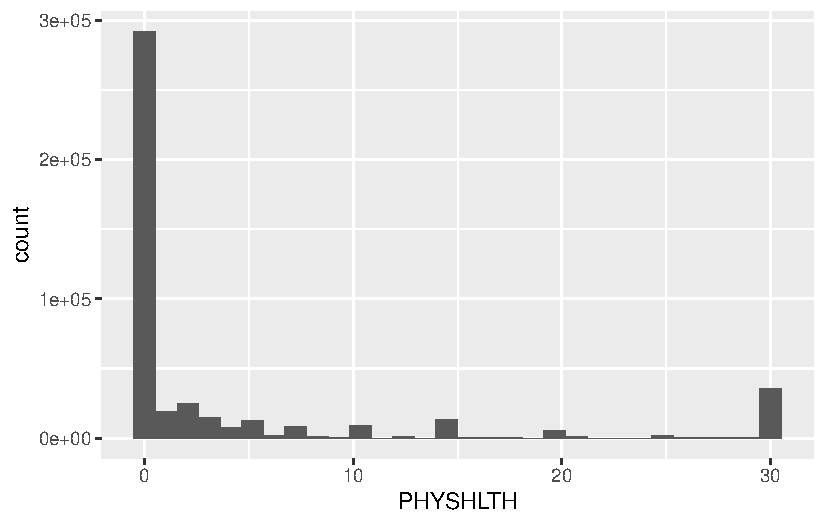
\includegraphics[keepaspectratio]{module2_files/figure-pdf/unnamed-chunk-67-1.pdf}}

\begin{Shaded}
\begin{Highlighting}[]
\CommentTok{\# Calculate Skewness and Kurtosis}
\FunctionTok{skew}\NormalTok{(brfss.cleaned}\SpecialCharTok{$}\NormalTok{PHYSHLTH)}
\end{Highlighting}
\end{Shaded}

\begin{verbatim}
skew (g1)        se         z         p 
    2.209     0.004   607.905     0.000 
\end{verbatim}

\begin{Shaded}
\begin{Highlighting}[]
\FunctionTok{kurtosis}\NormalTok{(brfss.cleaned}\SpecialCharTok{$}\NormalTok{PHYSHLTH)}
\end{Highlighting}
\end{Shaded}

\begin{verbatim}
Excess Kur (g2)              se               z               p 
          3.474           0.007         478.063           0.000 
\end{verbatim}

\begin{itemize}
\tightlist
\item
  The skew results provide a z of 607.905 (6.079054e+02) which is much
  higher than 7 (for large datasets). This indicates a clear right skew
  which means the data is not normally distributed.
\item
  The kurtosis results are also very leptokurtic. The z-score far
  exceeds the threshold of 7 for large samples, indicating extreme
  leptokurtosis (heavy tails). This is consistent with the right-skewed
  distribution seen in the histogram.
\end{itemize}

\subsubsection{Using Filters Example}\label{using-filters-example}

\begin{itemize}
\item
  Below takes an example of the brfss data to filter by certain variable
  statuses.

  \begin{itemize}
  \tightlist
  \item
    The first filter() chose observations that were any one of the three
    categories of transgender included in the data. Used the \textbar{}
    ``or'' operator for this filter().
  \item
    The second filter chose people in an age category above category 4
    but below category 12, in the age categories 5 through 11.
  \item
    The last filter used the !is.na to choose observations where HADMAM
    variable was not NA.
  \end{itemize}
\item
  Next, we reduce data set to contain only variables used to create
  table by using the select() command.
\item
  Next, we change all the remaining variables in data set to factors
  using mutate\_all() command. This not only changes the strings to
  factors, but also changes the numerical variables to factors.
\item
  Finally, we use mutate() commands to change the variable category to
  something meaningful(from the codebook).

  \begin{itemize}
  \tightlist
  \item
    Notice the backslash before the apostrophe in Don't in the X\_INCOMG
    recode. This is to prevent the .R file from ending the quotations.
    You could use double quotes around the statement to bypass this, or
    add the backslash like I did here.
  \end{itemize}

\begin{Shaded}
\begin{Highlighting}[]
\NormalTok{brfss\_small }\OtherTok{\textless{}{-}}\NormalTok{ brfss.cleaned }\SpecialCharTok{\%\textgreater{}\%}
    \FunctionTok{filter}\NormalTok{(TRNSGNDR }\SpecialCharTok{==} \StringTok{"Male to female"} \SpecialCharTok{|}\NormalTok{ TRNSGNDR }\SpecialCharTok{==} \StringTok{"Female to male"} \SpecialCharTok{|}
\NormalTok{        TRNSGNDR }\SpecialCharTok{==} \StringTok{"Gender non{-}conforming"}\NormalTok{) }\SpecialCharTok{\%\textgreater{}\%}
    \FunctionTok{filter}\NormalTok{(X\_AGEG5YR }\SpecialCharTok{\textgreater{}} \DecValTok{4} \SpecialCharTok{\&}\NormalTok{ X\_AGEG5YR }\SpecialCharTok{\textless{}} \DecValTok{12}\NormalTok{) }\SpecialCharTok{\%\textgreater{}\%}
    \FunctionTok{filter}\NormalTok{(}\SpecialCharTok{!}\FunctionTok{is.na}\NormalTok{(HADMAM)) }\SpecialCharTok{\%\textgreater{}\%}
    \FunctionTok{select}\NormalTok{(TRNSGNDR, X\_AGEG5YR, X\_RACE, X\_INCOMG, X\_EDUCAG, HLTHPLN1, HADMAM) }\SpecialCharTok{\%\textgreater{}\%}
    \FunctionTok{mutate\_all}\NormalTok{(as.factor) }\SpecialCharTok{\%\textgreater{}\%}
    \CommentTok{\# The next few mutates add labels to categorical variables based}
    \CommentTok{\# on the codebook.}
\FunctionTok{mutate}\NormalTok{(}\AttributeTok{X\_AGEG5YR =} \FunctionTok{recode\_factor}\NormalTok{(X\_AGEG5YR, }\StringTok{\textasciigrave{}}\AttributeTok{5}\StringTok{\textasciigrave{}} \OtherTok{=} \StringTok{"40{-}44"}\NormalTok{, }\StringTok{\textasciigrave{}}\AttributeTok{6}\StringTok{\textasciigrave{}} \OtherTok{=} \StringTok{"45{-}49"}\NormalTok{,}
    \StringTok{\textasciigrave{}}\AttributeTok{7}\StringTok{\textasciigrave{}} \OtherTok{=} \StringTok{"50{-}54"}\NormalTok{, }\StringTok{\textasciigrave{}}\AttributeTok{8}\StringTok{\textasciigrave{}} \OtherTok{=} \StringTok{"55{-}59"}\NormalTok{, }\StringTok{\textasciigrave{}}\AttributeTok{9}\StringTok{\textasciigrave{}} \OtherTok{=} \StringTok{"60{-}64"}\NormalTok{, }\StringTok{\textasciigrave{}}\AttributeTok{10}\StringTok{\textasciigrave{}} \OtherTok{=} \StringTok{"65{-}69"}\NormalTok{, }\StringTok{\textasciigrave{}}\AttributeTok{11}\StringTok{\textasciigrave{}} \OtherTok{=} \StringTok{"70{-}74"}\NormalTok{)) }\SpecialCharTok{\%\textgreater{}\%}
    \FunctionTok{mutate}\NormalTok{(}\AttributeTok{X\_INCOMG =} \FunctionTok{recode\_factor}\NormalTok{(X\_INCOMG, }\StringTok{\textasciigrave{}}\AttributeTok{1}\StringTok{\textasciigrave{}} \OtherTok{=} \StringTok{"Less than 15,000"}\NormalTok{,}
        \StringTok{\textasciigrave{}}\AttributeTok{2}\StringTok{\textasciigrave{}} \OtherTok{=} \StringTok{"15,000 to less than 25,000"}\NormalTok{, }\StringTok{\textasciigrave{}}\AttributeTok{3}\StringTok{\textasciigrave{}} \OtherTok{=} \StringTok{"25,000 to less than 35,000"}\NormalTok{,}
        \StringTok{\textasciigrave{}}\AttributeTok{4}\StringTok{\textasciigrave{}} \OtherTok{=} \StringTok{"35,000 to less than 50,000"}\NormalTok{, }\StringTok{\textasciigrave{}}\AttributeTok{5}\StringTok{\textasciigrave{}} \OtherTok{=} \StringTok{"50,000 or more"}\NormalTok{, }\StringTok{\textasciigrave{}}\AttributeTok{9}\StringTok{\textasciigrave{}} \OtherTok{=} \StringTok{"Don\textquotesingle{}t know/not sure/missing"}\NormalTok{)) }\SpecialCharTok{\%\textgreater{}\%}
    \FunctionTok{mutate}\NormalTok{(}\AttributeTok{X\_EDUCAG =} \FunctionTok{recode\_factor}\NormalTok{(X\_EDUCAG, }\StringTok{\textasciigrave{}}\AttributeTok{1}\StringTok{\textasciigrave{}} \OtherTok{=} \StringTok{"Did not graduate high school"}\NormalTok{,}
        \StringTok{\textasciigrave{}}\AttributeTok{2}\StringTok{\textasciigrave{}} \OtherTok{=} \StringTok{"Graduated high school"}\NormalTok{, }\StringTok{\textasciigrave{}}\AttributeTok{3}\StringTok{\textasciigrave{}} \OtherTok{=} \StringTok{"Attended college/technical school"}\NormalTok{,}
        \StringTok{\textasciigrave{}}\AttributeTok{4}\StringTok{\textasciigrave{}} \OtherTok{=} \StringTok{"Graduated from college/technical school"}\NormalTok{, }\StringTok{\textasciigrave{}}\AttributeTok{9}\StringTok{\textasciigrave{}} \OtherTok{=} \ConstantTok{NA\_character\_}\NormalTok{)) }\SpecialCharTok{\%\textgreater{}\%}
    \FunctionTok{mutate}\NormalTok{(}\AttributeTok{HLTHPLN1 =} \FunctionTok{recode\_factor}\NormalTok{(HLTHPLN1, }\StringTok{\textasciigrave{}}\AttributeTok{1}\StringTok{\textasciigrave{}} \OtherTok{=} \StringTok{"Yes"}\NormalTok{, }\StringTok{\textasciigrave{}}\AttributeTok{2}\StringTok{\textasciigrave{}} \OtherTok{=} \StringTok{"No"}\NormalTok{,}
        \StringTok{\textasciigrave{}}\AttributeTok{7}\StringTok{\textasciigrave{}} \OtherTok{=} \StringTok{"Don\textquotesingle{}t know/not sure/missing"}\NormalTok{, }\StringTok{\textasciigrave{}}\AttributeTok{9}\StringTok{\textasciigrave{}} \OtherTok{=} \StringTok{"Refused"}\NormalTok{)) }\SpecialCharTok{\%\textgreater{}\%}
    \FunctionTok{mutate}\NormalTok{(}\AttributeTok{X\_RACE =} \FunctionTok{recode\_factor}\NormalTok{(X\_RACE, }\StringTok{\textasciigrave{}}\AttributeTok{1}\StringTok{\textasciigrave{}} \OtherTok{=} \StringTok{"White"}\NormalTok{, }\StringTok{\textasciigrave{}}\AttributeTok{2}\StringTok{\textasciigrave{}} \OtherTok{=} \StringTok{"Black"}\NormalTok{,}
        \StringTok{\textasciigrave{}}\AttributeTok{3}\StringTok{\textasciigrave{}} \OtherTok{=} \StringTok{"Native American"}\NormalTok{, }\StringTok{\textasciigrave{}}\AttributeTok{4}\StringTok{\textasciigrave{}} \OtherTok{=} \StringTok{"Asian/Pacific Islander"}\NormalTok{, }\StringTok{\textasciigrave{}}\AttributeTok{5}\StringTok{\textasciigrave{}} \OtherTok{=} \StringTok{"Other"}\NormalTok{,}
        \StringTok{\textasciigrave{}}\AttributeTok{6}\StringTok{\textasciigrave{}} \OtherTok{=} \StringTok{"Other"}\NormalTok{, }\StringTok{\textasciigrave{}}\AttributeTok{7}\StringTok{\textasciigrave{}} \OtherTok{=} \StringTok{"Other"}\NormalTok{, }\StringTok{\textasciigrave{}}\AttributeTok{8}\StringTok{\textasciigrave{}} \OtherTok{=} \StringTok{"Other"}\NormalTok{, }\StringTok{\textasciigrave{}}\AttributeTok{9}\StringTok{\textasciigrave{}} \OtherTok{=} \StringTok{"Other"}\NormalTok{))}
\CommentTok{\# print a summary}
\FunctionTok{summary}\NormalTok{(brfss\_small)}
\end{Highlighting}
\end{Shaded}

\begin{verbatim}
                  TRNSGNDR   X_AGEG5YR                     X_RACE   
 Male to female       : 77   40-44:27   White                 :152  
 Female to male       :113   45-49:27   Black                 : 31  
 Gender non-conforming: 32   50-54:32   Native American       :  4  
 Not transgender      :  0   55-59:44   Asian/Pacific Islander:  6  
 Not sure             :  0   60-64:44   Other                 : 29  
 Refused              :  0   65-69:24                               
                             70-74:24                               
                        X_INCOMG                                     X_EDUCAG 
 Less than 15,000           :46   Did not graduate high school           :24  
 15,000 to less than 25,000 :44   Graduated high school                  :86  
 25,000 to less than 35,000 :19   Attended college/technical school      :68  
 35,000 to less than 50,000 :26   Graduated from college/technical school:44  
 50,000 or more             :65                                               
 Don't know/not sure/missing:22                                               

 HLTHPLN1  HADMAM 
 Yes:198   1:198  
 No : 24   2: 22  
           9:  2  



\end{verbatim}
\item
  This data set full of categorical variables is now fully cleaned and
  ready to be analyzed!
\end{itemize}

\bookmarksetup{startatroot}

\chapter{Using AI}\label{using-ai-1}

Use the following prompts on a generative AI, like chatGPT, to learn
more about descriptive statistics.

\begin{itemize}
\item
  What is the difference between mean, median, and mode in describing
  data distributions, and how can each be used to understand the shape
  of a distribution? * How do mean and median help identify whether a
  distribution is skewed, and what does it tell us about the dataset?
\item
  Can you explain how the mean, median, and mode behave in normal,
  positively skewed, and negatively skewed distributions?
\item
  What are standard deviation (SD) and variance, and how do they measure
  the spread of data in a distribution?
\item
  Explain the differences between range, interquartile range (IQR), and
  standard deviation in describing the variability in a dataset.
\item
  How does a high standard deviation or variance affect the
  interpretation of a dataset compared to a low standard deviation?
\item
  What is skewness, and how does it affect the shape of a distribution?
  How can we identify positive and negative skew?
\item
  How is kurtosis defined in the semTools package in R, and what does it
  tell us about the tails of a distribution?
\item
  How would you compare and contrast the roles of skewness and kurtosis
  in identifying the shape and behavior of a distribution?
\item
  How can you use the filter() function to subset a dataset based on
  multiple conditions using \& and \textbar{} in R?
\item
  How does subsetting using square brackets {[}{]} differ from using the
  filter() function in R?
\item
  How does the mutate() function help in transforming and creating new
  variables, and what are some practical examples?''
\item
  What is the purpose of the group\_by() function, and how does it
  interact with summarize() to create summary statistics in R?''
\item
  Explain how you can use arrange() to sort a dataset by one or more
  variables and demonstrate sorting both in ascending and descending
  order.''
\item
  Why is the piping operator \%\textgreater\% useful in R, and how does
  it improve the readability and structure of your code?
\item
  How would you use summarize() to calculate mean, median, and standard
  deviation for a numerical variable in R?
\end{itemize}

\bookmarksetup{startatroot}

\chapter{Summary}\label{summary-2}

\begin{itemize}
\tightlist
\item
  In this lesson, we worked through descriptive statistics including
  skewness and kurtosis. We learned about variables and scales of
  measurement, how to summarize qualitative and quantitative data.
\item
  We then worked through the basics on data cleaning. Data cleaning is
  so important and there are so many ways to do it. Provided are some
  examples using popular functions in dplyr (under tidyverse).
\end{itemize}

\bookmarksetup{startatroot}

\chapter{Module 3: Data
Visualization}\label{module-3-data-visualization}

\begin{itemize}
\tightlist
\item
  The goal of this lesson is to be able to create visualizations that
  help describe a variable or variables more easily (descriptive
  statistics) and to explore patterns in the data based on groups or
  between two or more variables (exploratory data analysis).
\end{itemize}

\subsection{At a Glance}\label{at-a-glance-2}

\begin{itemize}
\item
  In order to succeed in this lesson, we need to learn how to visualize
  data, noting that there are many ways to do this in R. This lesson
  presents common graphs used in R, and focuses on using ggplot2, a very
  common graphics package that is part of the tidyverse.
\item
  Because packages evolve fairly quickly, parameters within the commands
  shown in this section could evolve and adjust. The best way to figure
  out how to fine-tune your new graph is to explore options and
  parameter settings, while also using the open-source community.
\item
  By the end of this lesson, you should be able to create the following:
\end{itemize}

\begin{enumerate}
\def\labelenumi{\arabic{enumi}.}
\tightlist
\item
  Common Graphs for a Single \emph{Categorical} Variable
\item
  Common Graphs for a Single \emph{Continuous} Variable
\item
  Common Graphs for Two Variables at Once
\end{enumerate}

\begin{itemize}
\tightlist
\item
  This lesson does not provide an exhaustive list of what you can do in
  R, but is a good starting point presenting some of the top graphs used
  in statistics with some common parameters added in.
\end{itemize}

\subsection{Lesson Objectives}\label{lesson-objectives-2}

\begin{itemize}
\tightlist
\item
  Choose and create graphs for a single categorical variable.
\item
  Choose and create graphs for a single continuous variable.
\item
  Choose and create graphs for two variables at once.
\end{itemize}

\subsection{Consider While Reading}\label{consider-while-reading-2}

\begin{itemize}
\item
  It is extremely useful to graph data in R in order to visualize what
  the data is telling us.
\item
  When making graphs, there are a lot of ways to visualize data
  correctly, but there are just as many to do it incorrectly. Be careful
  not to force the data into the story you want it to tell.
\item
  Always be cautious when looking at visuals to make sure the data was
  handled properly.
\item
  The lesson is arranged by first evaluating the variable or variables
  of interest by data type (categorical or quantitative) and then giving
  some examples of visualizations where this is commonly used. It is
  essential to make sure the variable is in the right data type before
  you create a chart. We look at many charts in this lesson including
  bar charts, density plots, boxplots and scatterplots. A multiple
  boxplot helps us understand the relationship between a grouping
  variable and a numerical variable. The scatterplot helps us understand
  if there is a relationship between two numerical variables and it
  helps us determine whether that relationship is linear or nonlinear.
\item
  A lot of graphs you can do in ggplot, you can also do with base R.
  However, ggplot has much more capability to customize a specific
  format for your graphic.

  \begin{itemize}
  \tightlist
  \item
    Base R has many options to graph a variable or variables. If all you
    want is some insight into the data, this might be the way to go.
  \item
    ggplot2 is extremely popular graphing package and has a good pattern
    for making charts. You set the first layer with the ggplot() command
    and then add layers as needed for your graphic.
  \item
    There are also other graphing packages that serve a specific purpose
    (i.e., waffle package in R).
  \end{itemize}
\end{itemize}

\section{Layering in ggplot}\label{layering-in-ggplot}

\begin{itemize}
\tightlist
\item
  Layering is a fundamental concept in ggplot2 that allows you to build
  complex visualizations by adding different components (or ``layers'')
  on top of each other. Each layer in a ggplot2 plot can represent
  different types of data, aesthetics, or annotations, enabling
  flexibility and control over how data is visualized. Layers can
  include geometries (e.g., points, lines, bars), statistical summaries,
  labels, grids, and themes.
\item
  Separation of Plot Components: Each layer can handle a different part
  of the plot. For example, one layer may be used for bars, another for
  labels, and another for a trend line. This allows you to build up a
  plot step by step.
\item
  Customization and Enhancement: By adding multiple layers, you can
  customize different aspects of the plot such as labels, colors,
  annotations, and theme elements. Each layer can be independently
  controlled.
\item
  Modularity: Layering allows you to modularize your plot construction,
  making it easier to add, remove, or modify parts of the plot without
  changing the entire structure.
\item
  Combining Data Sources: Different layers can use different datasets or
  aesthetics, which is useful when you need to overlay one dataset on
  top of another (e.g., adding a regression line over a scatter plot).
\end{itemize}

\section{Graphs for a Single Categorical
Variable}\label{graphs-for-a-single-categorical-variable}

\begin{itemize}
\tightlist
\item
  A categorical variable has categories that are either ordinal with a
  logical order or nominal with no logical order.
\item
  Categorical variables need to be set as the factor data type in R to
  be able to be analyzed and visualized correctly.
\item
  Some common graphing options for single categorical variable:

  \begin{enumerate}
  \def\labelenumi{\arabic{enumi}.}
  \tightlist
  \item
    Bar graph
  \item
    Pie chart
  \end{enumerate}
\item
  In any graph, it is beneficial to do any data cleaning and
  investigation into the variable(s) before you begin. With categorical
  variables, this may require recoding the factor(s) of interest and
  possibly renaming it/them to something meaningful if needed.
\end{itemize}

\subsection{Bar Graph}\label{bar-graph}

\begin{itemize}
\tightlist
\item
  A bar graph depicts the frequency or the relative frequency for each
  category of the qualitative data as a bar rising vertically from the
  horizontal axis. A bar graph is also known as a bar chart and is often
  used to examine similarities and differences across categories of
  things; bars can represent frequencies, percentages, means, or other
  statistics.
\item
  We can learn a lot from a bar graph, like the marital status group
  with the highest and lowest frequencies according to the census.gov.
\end{itemize}

\pandocbounded{
\includegraphics[keepaspectratio]{module3_files/figure-pdf/unnamed-chunk-2-1.pdf}}

\subsubsection{geom\_bar()}\label{geom_bar}

\begin{itemize}
\tightlist
\item
  Create a Bar Graph using ggplot() Command
\item
  Like histograms, ggplot has many more parameters available over base R
  to construct bar graphs.
\item
  First, we load tidyerse to access ggplot() command and others. You can
  always do this at the start of all your code to keep all the libraries
  together that are being used.
\end{itemize}

\begin{Shaded}
\begin{Highlighting}[]
\FunctionTok{library}\NormalTok{(}\StringTok{"tidyverse"}\NormalTok{)}
\end{Highlighting}
\end{Shaded}

\begin{itemize}
\tightlist
\item
  ggplot() works in layers, so you will routinely see the \emph{+}
  symbol to kick off a new layer with added functionality.
\item
  Using the ggplot, we always include the aes() command first inside the
  ggplot() command. The aes() command is a \emph{quoting function} that
  describes the variables being used. From there, it depends on the
  plot.

  \begin{itemize}
  \tightlist
  \item
    First layer: ggplot() and aes() which calls the dataset and
    variables used.
  \item
    Second layer: Graph type: Bar graph: geom\_bar().
  \item
    Additional layers: labs - for labels including titles; themes; and
    geom\_text. Recreate the example below adding one layer at a time to
    see how the visualization changes.
  \end{itemize}
\end{itemize}

\subsubsection{Pertinent Parameters to the
geom\_bar()}\label{pertinent-parameters-to-the-geom_bar}

\begin{itemize}
\tightlist
\item
  \textbf{stat=``identity''}: In ggplot2, the argument
  \emph{stat=``identity''} is used inside the geom\_bar when creating
  bar charts to specify that the actual values of the data should be
  plotted, rather than calculated summary statistics. By default, ggplot
  assumes that bar charts use stat=``count'', which counts the number of
  observations in each category. When you want to display the actual
  values in your dataset (e.g., sales numbers, average scores), you need
  to set stat=``identity'' to ensure that the y-values are mapped
  directly from the data rather than being automatically counted.
\item
  \textbf{position=``dodge''}: If we have more than one categorical
  variable, we might set the \emph{position=``dodge''} argument. This
  argument controls how the bars are positioned relative to each other
  when you are plotting multiple categories within a bar chart. By
  default, bars in a bar chart are stacked, and setting
  position=``dodge'' ensures that they are placed side-by-side. This is
  particularly useful when you are comparing multiple groups or
  categories within the same plot, as it allows for a clear visual
  distinction between each group. In the example below, we only have one
  variable, so position=``dodge'' argument is not needed.\\
\item
  In combination, using \emph{stat=``identity''} and
  \emph{position=``dodge''} is common when you want to compare different
  categories or groups with specific values in a side-by-side manner,
  ensuring the chart is easy to interpret. For example, if you are
  comparing sales figures across different products for multiple years,
  this approach would give you a bar for each product in each year,
  clearly separated.
\item
  \textbf{show.legend = FALSE}: In ggplot2, the argument
  \emph{show.legend = FALSE} is used to hide the legend for a particular
  layer or the entire plot. By default, ggplot2 automatically adds a
  legend if you include aesthetics like color, size, or shape that
  distinguish groups in your data. If you don't want the legend to
  appear, you can set show.legend = FALSE.
\item
  \textbf{scale\_fill\_manual():} When creating grouped bar charts or
  other plots with multiple categories, it's important to ensure that
  the visual distinction between groups is clear. This is where manually
  setting the colors for each category comes into play. The
  \emph{scale\_fill\_manual()} function in ggplot2 allows you to
  manually define the colors used for the filled areas, such as the bars
  in a bar chart or the shaded areas in an area chart. By using the
  values argument within scale\_fill\_manual(), you can specify a custom
  color palette that suits your design or presentation needs. For
  example, you might choose a palette of yellow and brown to represent
  different categories. A key aspect of using scale\_fill\_manual()
  effectively is knowing how many colors to provide. The number of
  colors you define in the values argument must match the number of
  levels or categories in your data. If you are comparing three product
  categories, for instance, you'll need to provide exactly three
  colors---one for each category. Failing to match the number of colors
  to the number of categories can result in errors or misrepresentation
  in the plot. For example, if you have four levels (e.g., four
  different product categories or groups) and only provide two colors,
  ggplot may not know how to properly assign colors to the additional
  categories. Therefore, it's crucial to know the number of distinct
  categories in your data and plan your color palette accordingly to
  maintain clarity and visual consistency in your chart.
\end{itemize}

\begin{Shaded}
\begin{Highlighting}[]
\DocumentationTok{\#\# inputting probabilities calculated from a 2023 multiple choice}
\DocumentationTok{\#\# question.  From what you learned about R so far, how do you expect}
\DocumentationTok{\#\# its market share to change?}
\NormalTok{GoUp }\OtherTok{\textless{}{-}} \FloatTok{0.54285}
\NormalTok{GoDown }\OtherTok{\textless{}{-}} \FloatTok{0.03809}
\NormalTok{RemainStable }\OtherTok{\textless{}{-}} \FloatTok{0.34285}
\NormalTok{NoOpinion }\OtherTok{\textless{}{-}} \FloatTok{0.07619}
\CommentTok{\# designing the data frame}
\NormalTok{data\_frame }\OtherTok{\textless{}{-}} \FunctionTok{data.frame}\NormalTok{(}\AttributeTok{Category =} \FunctionTok{c}\NormalTok{(}\StringTok{"Go Up"}\NormalTok{, }\StringTok{"Go Down"}\NormalTok{, }\StringTok{"Remain Stable"}\NormalTok{,}
    \StringTok{"No Opinion"}\NormalTok{), }\AttributeTok{Percentage =} \FunctionTok{c}\NormalTok{(GoUp, GoDown, RemainStable, NoOpinion))}
\CommentTok{\# Making the graph}
\NormalTok{MarketShare }\OtherTok{\textless{}{-}} \FunctionTok{ggplot}\NormalTok{(data\_frame, }\FunctionTok{aes}\NormalTok{(}\AttributeTok{x =}\NormalTok{ Category, }\AttributeTok{y =}\NormalTok{ Percentage, }\AttributeTok{fill =}\NormalTok{ Category)) }\SpecialCharTok{+}
    \FunctionTok{geom\_bar}\NormalTok{(}\AttributeTok{stat =} \StringTok{"identity"}\NormalTok{, }\AttributeTok{show.legend =} \ConstantTok{FALSE}\NormalTok{) }\SpecialCharTok{+} \FunctionTok{labs}\NormalTok{(}\AttributeTok{title =} \StringTok{"How do you expect R\textquotesingle{}s market share to change?"}\NormalTok{,}
    \AttributeTok{x =} \StringTok{"Opinion Category"}\NormalTok{, }\AttributeTok{y =} \StringTok{"Percentage (\%)"}\NormalTok{) }\SpecialCharTok{+} \FunctionTok{theme\_minimal}\NormalTok{() }\SpecialCharTok{+} \FunctionTok{geom\_text}\NormalTok{(}\FunctionTok{aes}\NormalTok{(}\AttributeTok{label =}\NormalTok{ Percentage),}
    \AttributeTok{vjust =} \SpecialCharTok{{-}}\FloatTok{0.5}\NormalTok{, }\AttributeTok{size =} \DecValTok{4}\NormalTok{) }\SpecialCharTok{+} \FunctionTok{scale\_fill\_manual}\NormalTok{(}\AttributeTok{values =} \FunctionTok{c}\NormalTok{(}\StringTok{"red"}\NormalTok{, }\StringTok{"blue"}\NormalTok{,}
    \StringTok{"purple"}\NormalTok{, }\StringTok{"green"}\NormalTok{))}

\NormalTok{MarketShare}
\end{Highlighting}
\end{Shaded}

\pandocbounded{
\includegraphics[keepaspectratio]{module3_files/figure-pdf/unnamed-chunk-4-1.pdf}}

\subsection{Bar Graph with Data
Wrangling}\label{bar-graph-with-data-wrangling}

\begin{itemize}
\tightlist
\item
  Let's start an example from scratch so that we can see each parameter
  take effect. In doing so, lets use a dataset to make a bar graph
  instead of relying on pre-calculated data.\\
\item
  Lets examine the AUQ300 variable from the nhanes survey to run an
  example.
\end{itemize}

\begin{Shaded}
\begin{Highlighting}[]
\NormalTok{nhanes }\OtherTok{\textless{}{-}} \FunctionTok{read.csv}\NormalTok{(}\StringTok{"data/nhanes2012.csv"}\NormalTok{)}
\end{Highlighting}
\end{Shaded}

\begin{itemize}
\tightlist
\item
  Next, we need to check the import by looking at the summary or head of
  the data.
\end{itemize}

\begin{Shaded}
\begin{Highlighting}[]
\CommentTok{\# Results hidden to save space, but gives you the first 6 records in}
\CommentTok{\# the data set.}
\FunctionTok{head}\NormalTok{(nhanes)}
\end{Highlighting}
\end{Shaded}

\begin{itemize}
\tightlist
\item
  We can also check the summary of data of only the variable of
  interest, AUQ300, to get a sense of what we are evaluating.
\end{itemize}

\begin{Shaded}
\begin{Highlighting}[]
\FunctionTok{summary}\NormalTok{(nhanes}\SpecialCharTok{$}\NormalTok{AUQ300)}
\end{Highlighting}
\end{Shaded}

\begin{verbatim}
   Min. 1st Qu.  Median    Mean 3rd Qu.    Max.    NA's 
  1.000   1.000   2.000   1.656   2.000   7.000    4689 
\end{verbatim}

\begin{itemize}
\tightlist
\item
  The AUQ300 variable represents gun use. A screenshot of the codebook
  is copied below so that we can see what AUQ300 really refers to. It is
  available on https://wwwn.cdc.gov/Nchs/Nhanes/2011-2012/AUQ\_G.htm.
  This is always a necessary step because variable names can be
  convoluted and not representative of the variable definition.
\end{itemize}

\begin{figure}[H]

{\centering \pandocbounded{\includegraphics[keepaspectratio]{Pictures/Ch3/AUQ300.png}}

}

\caption{AUQ300}

\end{figure}%

\subsubsection{Recode Variable if
Needed}\label{recode-variable-if-needed}

\begin{itemize}
\tightlist
\item
  Look to see if the AUQ300 needs recoding after looking at the codebook
  and making sense of the variable.
\item
  AUQ300 needs to be a factor variable with 1 equaling a \emph{Yes} and
  2 equaling a \emph{No}. We can use recode\_factor to accomplish 2
  things at once with the mutate function.
\item
  recode\_factor() transforms the levels of a categorical variable
  (factor) into a new set of levels and is specific to categorical
  variables.
\item
  recode() is generic and can apply to numerical, categorical, or
  textual data, but still transforms data from one format or code to
  another.
\end{itemize}

\begin{Shaded}
\begin{Highlighting}[]
\NormalTok{nhanes.clean }\OtherTok{\textless{}{-}}\NormalTok{ nhanes }\SpecialCharTok{\%\textgreater{}\%}
    \FunctionTok{select}\NormalTok{(AUQ300) }\SpecialCharTok{\%\textgreater{}\%}
    \FunctionTok{mutate}\NormalTok{(}\AttributeTok{AUQ300 =} \FunctionTok{recode\_factor}\NormalTok{(AUQ300, }\StringTok{\textasciigrave{}}\AttributeTok{1}\StringTok{\textasciigrave{}} \OtherTok{=} \StringTok{"Yes"}\NormalTok{, }\StringTok{\textasciigrave{}}\AttributeTok{2}\StringTok{\textasciigrave{}} \OtherTok{=} \StringTok{"No"}\NormalTok{))}
\end{Highlighting}
\end{Shaded}

\begin{itemize}
\tightlist
\item
  Then, we need to check the recode for accuracy. You should see the
  No's and Yes's alongside the rest being coded as NA's.
\end{itemize}

\begin{Shaded}
\begin{Highlighting}[]
\FunctionTok{summary}\NormalTok{(nhanes.clean)}
\end{Highlighting}
\end{Shaded}

\begin{verbatim}
  AUQ300    
 Yes :1613  
 No  :3061  
 NA's:4690  
\end{verbatim}

\subsubsection{Get Bar Roughly Plotted}\label{get-bar-roughly-plotted}

\begin{itemize}
\item
  Start with the basic plot using the ggplot() and geom\_bar() commands.
\item
  Below writes the statement with and without the piping operator.

  \begin{itemize}
  \tightlist
  \item
    Since we are also going to use data preparation techniques, the
    piping operator is recommended.
  \end{itemize}

\begin{Shaded}
\begin{Highlighting}[]
\CommentTok{\# Without piping operator}
\FunctionTok{ggplot}\NormalTok{(nhanes.clean, }\FunctionTok{aes}\NormalTok{(}\AttributeTok{x =}\NormalTok{ AUQ300)) }\SpecialCharTok{+} \FunctionTok{geom\_bar}\NormalTok{()}
\end{Highlighting}
\end{Shaded}

  \pandocbounded{
\includegraphics[keepaspectratio]{module3_files/figure-pdf/unnamed-chunk-10-1.pdf}}

\begin{Shaded}
\begin{Highlighting}[]
\CommentTok{\# With piping operator}
\NormalTok{nhanes.clean }\SpecialCharTok{\%\textgreater{}\%}
    \FunctionTok{ggplot}\NormalTok{(}\FunctionTok{aes}\NormalTok{(}\AttributeTok{x =}\NormalTok{ AUQ300)) }\SpecialCharTok{+} \FunctionTok{geom\_bar}\NormalTok{()}
\end{Highlighting}
\end{Shaded}

  \pandocbounded{
\includegraphics[keepaspectratio]{module3_files/figure-pdf/unnamed-chunk-10-2.pdf}}
\end{itemize}

\subsubsection{Add Functions to Clean
Chart}\label{add-functions-to-clean-chart}

\begin{itemize}
\tightlist
\item
  Omit the NA category from AUQ300 variable, which represents gun use.
  Then plot the graph below.
\item
  The drop\_na() function is a good way to drop NA values from either
  the entire dataset or just one variable. It was introduced in the data
  prep lesson. Since we are only interested in dropping NA values from
  our one variable of interest that is to be graphed (AUQ300), we can
  put it in the parentheses so that we do not unintentionally drop lots
  of observations for no reason.
\item
  Add an axis labels under \emph{labs(x = \ldots, y=\ldots)}.
\end{itemize}

\begin{Shaded}
\begin{Highlighting}[]
\NormalTok{nhanes.clean }\SpecialCharTok{\%\textgreater{}\%}
  \FunctionTok{drop\_na}\NormalTok{(AUQ300) }\SpecialCharTok{\%\textgreater{}\%}
  \FunctionTok{ggplot}\NormalTok{(}\FunctionTok{aes}\NormalTok{(}\AttributeTok{x =}\NormalTok{ AUQ300)) }\SpecialCharTok{+} \FunctionTok{geom\_bar}\NormalTok{() }\SpecialCharTok{+}
  \FunctionTok{labs}\NormalTok{(}\AttributeTok{x =} \StringTok{"Gun use"}\NormalTok{, }\AttributeTok{y =} \StringTok{"Number of participants"}\NormalTok{)}
\end{Highlighting}
\end{Shaded}

\pandocbounded{
\includegraphics[keepaspectratio]{module3_files/figure-pdf/unnamed-chunk-11-1.pdf}}

\begin{Shaded}
\begin{Highlighting}[]
\DocumentationTok{\#\#Here, we really benefit from the piping operator because we are doing more than one thing.}
\end{Highlighting}
\end{Shaded}

\begin{itemize}
\tightlist
\item
  From the bar graph, we can see that almost double the amount of people
  have not fired a firearm for any reason than those that fired one.
\end{itemize}

\subsubsection{Adding Color}\label{adding-color}

\begin{itemize}
\item
  There are many ways to add color to a bar graph. Below, the color is
  filled in directly in the aes() command by choosing it to give a
  different color to each categorical value of AUQ300.

  \begin{itemize}
  \tightlist
  \item
    When fill is mapped to a variable, the fill color of the geom will
    vary based on the values of that variable. This is useful for
    distinguishing different groups or categories within the data. In
    this case the fill=AUQ300 gives a distinct color pattern based on
    how many categories there are considering the fact we are using the
    default ``scale.''
  \end{itemize}

\begin{Shaded}
\begin{Highlighting}[]
\NormalTok{nhanes.clean }\SpecialCharTok{\%\textgreater{}\%}
  \FunctionTok{drop\_na}\NormalTok{(AUQ300) }\SpecialCharTok{\%\textgreater{}\%}
  \FunctionTok{ggplot}\NormalTok{(}\FunctionTok{aes}\NormalTok{(AUQ300, }\AttributeTok{fill=}\NormalTok{AUQ300)) }\SpecialCharTok{+}
  \FunctionTok{geom\_bar}\NormalTok{() }\SpecialCharTok{+}
  \FunctionTok{labs}\NormalTok{(}\AttributeTok{x =} \StringTok{"Gun use"}\NormalTok{, }\AttributeTok{y =} \StringTok{"Number of participants"}\NormalTok{, }
       \AttributeTok{subtitle =} \StringTok{"Filled inside the aes()"}\NormalTok{) }
\end{Highlighting}
\end{Shaded}

  \pandocbounded{
\includegraphics[keepaspectratio]{module3_files/figure-pdf/unnamed-chunk-12-1.pdf}}
\end{itemize}

\subsubsection{Data Prep and Then
Visualized}\label{data-prep-and-then-visualized}

\begin{itemize}
\item
  In the command below, we create a gss.2016.cleaned object to make a
  barplot. In doing so, we do the following:
\item
  Create a bar graph using the ggplot() command, which requires an aes()
  quoting function. This function says that we want to use the grass
  variable in our bar graph.
\item
  Drop all NAs from the grass variable so that legal and not legal are
  the only categories.
\item
  We then create the bars and fill them with 2 colors, red and purple.
  Many color codes can be used here, and will be discussed in a later
  lesson.
\item
  We then add labels to our graph on both x and y axis.
\item
  Finally, we print the new graph, which is saved under the legalize.bar
  object.
\item
  Below, I brought back over the code from the last part in Data
  Preparation. You should still have this in your Chapter1.R file. We
  are going to use that file to create a graphics in R.
\end{itemize}

\begin{Shaded}
\begin{Highlighting}[]
\NormalTok{gss}\FloatTok{.2016} \OtherTok{\textless{}{-}} \FunctionTok{read\_csv}\NormalTok{(}\AttributeTok{file =} \StringTok{"data/gss2016.csv"}\NormalTok{)}
\NormalTok{gss.}\FloatTok{2016.}\NormalTok{cleaned }\OtherTok{\textless{}{-}}\NormalTok{ gss}\FloatTok{.2016} \SpecialCharTok{\%\textgreater{}\%}
    \FunctionTok{mutate}\NormalTok{(}\AttributeTok{grass =} \FunctionTok{as.factor}\NormalTok{(grass)) }\SpecialCharTok{\%\textgreater{}\%}
    \FunctionTok{mutate}\NormalTok{(}\AttributeTok{grass =} \FunctionTok{na\_if}\NormalTok{(}\AttributeTok{x =}\NormalTok{ grass, }\AttributeTok{y =} \StringTok{"DK"}\NormalTok{)) }\SpecialCharTok{\%\textgreater{}\%}
    \FunctionTok{mutate}\NormalTok{(}\AttributeTok{grass =} \FunctionTok{na\_if}\NormalTok{(}\AttributeTok{x =}\NormalTok{ grass, }\AttributeTok{y =} \StringTok{"IAP"}\NormalTok{)) }\SpecialCharTok{\%\textgreater{}\%}
    \FunctionTok{mutate}\NormalTok{(}\AttributeTok{grass =} \FunctionTok{droplevels}\NormalTok{(}\AttributeTok{x =}\NormalTok{ grass)) }\SpecialCharTok{\%\textgreater{}\%}
    \FunctionTok{mutate}\NormalTok{(}\AttributeTok{age =} \FunctionTok{recode}\NormalTok{(age, }\StringTok{\textasciigrave{}}\AttributeTok{89 OR OLDER}\StringTok{\textasciigrave{}} \OtherTok{=} \StringTok{"89"}\NormalTok{)) }\SpecialCharTok{\%\textgreater{}\%}
    \FunctionTok{mutate}\NormalTok{(}\AttributeTok{age =} \FunctionTok{as.numeric}\NormalTok{(}\AttributeTok{x =}\NormalTok{ age)) }\SpecialCharTok{\%\textgreater{}\%}
    \FunctionTok{mutate}\NormalTok{(}\AttributeTok{age.cat =} \FunctionTok{cut}\NormalTok{(}\AttributeTok{x =}\NormalTok{ age, }\AttributeTok{breaks =} \FunctionTok{c}\NormalTok{(}\SpecialCharTok{{-}}\ConstantTok{Inf}\NormalTok{, }\DecValTok{29}\NormalTok{, }\DecValTok{59}\NormalTok{, }\DecValTok{74}\NormalTok{, }\ConstantTok{Inf}\NormalTok{), }\AttributeTok{labels =} \FunctionTok{c}\NormalTok{(}\StringTok{"\textless{} 30"}\NormalTok{,}
        \StringTok{"30 {-} 59"}\NormalTok{, }\StringTok{"60 {-} 74"}\NormalTok{, }\StringTok{"75+"}\NormalTok{)))}
\end{Highlighting}
\end{Shaded}

\begin{itemize}
\tightlist
\item
  Once the data is prepped, we can graph the variable or variables.
\end{itemize}

\begin{Shaded}
\begin{Highlighting}[]
\FunctionTok{ggplot}\NormalTok{(gss.}\FloatTok{2016.}\NormalTok{cleaned, }\FunctionTok{aes}\NormalTok{(grass)) }\SpecialCharTok{+} \FunctionTok{geom\_bar}\NormalTok{()  }\DocumentationTok{\#\#with no piping operator}
\end{Highlighting}
\end{Shaded}

\pandocbounded{\includegraphics[keepaspectratio]{module3_files/figure-pdf/unnamed-chunk-14-1.pdf}}

\begin{Shaded}
\begin{Highlighting}[]
\NormalTok{gss.}\FloatTok{2016.}\NormalTok{cleaned }\SpecialCharTok{\%\textgreater{}\%}
    \FunctionTok{ggplot}\NormalTok{(}\FunctionTok{aes}\NormalTok{(grass)) }\SpecialCharTok{+} \FunctionTok{geom\_bar}\NormalTok{()  }\DocumentationTok{\#\#with piping operator}
\end{Highlighting}
\end{Shaded}

\pandocbounded{\includegraphics[keepaspectratio]{module3_files/figure-pdf/unnamed-chunk-14-2.pdf}}

\begin{Shaded}
\begin{Highlighting}[]
\CommentTok{\# Make a Bar Graph for Grass Variable}
\NormalTok{gss.}\FloatTok{2016.}\NormalTok{cleaned }\SpecialCharTok{\%\textgreater{}\%}
    \FunctionTok{drop\_na}\NormalTok{() }\SpecialCharTok{\%\textgreater{}\%}
    \FunctionTok{ggplot}\NormalTok{(}\FunctionTok{aes}\NormalTok{(grass)) }\SpecialCharTok{+} \FunctionTok{geom\_bar}\NormalTok{(}\AttributeTok{fill =} \FunctionTok{c}\NormalTok{(}\StringTok{"red"}\NormalTok{, }\StringTok{"blue"}\NormalTok{)) }\SpecialCharTok{+} \FunctionTok{labs}\NormalTok{(}\AttributeTok{x =} \StringTok{"Should marijuana be legal"}\NormalTok{,}
    \AttributeTok{y =} \StringTok{"Frequency of Responses"}\NormalTok{)}
\end{Highlighting}
\end{Shaded}

\pandocbounded{
\includegraphics[keepaspectratio]{module3_files/figure-pdf/unnamed-chunk-15-1.pdf}}

\subsubsection{Edit The Graphic}\label{edit-the-graphic}

\begin{itemize}
\tightlist
\item
  Next, we can edit these commands to include the age variable. The
  aes() quoting function has expanded to have the bars filled color
  using the grass variable, the age category has replaced the grass
  variable on the x axis.
\end{itemize}

\begin{Shaded}
\begin{Highlighting}[]
\NormalTok{gss.}\FloatTok{2016.}\NormalTok{cleaned }\SpecialCharTok{\%\textgreater{}\%}
    \FunctionTok{drop\_na}\NormalTok{() }\SpecialCharTok{\%\textgreater{}\%}
    \FunctionTok{ggplot}\NormalTok{(}\FunctionTok{aes}\NormalTok{(age.cat, }\AttributeTok{fill =}\NormalTok{ grass)) }\SpecialCharTok{+} \FunctionTok{geom\_bar}\NormalTok{() }\SpecialCharTok{+} \FunctionTok{labs}\NormalTok{(}\AttributeTok{x =} \StringTok{"Age Category"}\NormalTok{,}
    \AttributeTok{y =} \StringTok{"Frequency of responses"}\NormalTok{)}
\end{Highlighting}
\end{Shaded}

\pandocbounded{\includegraphics[keepaspectratio]{module3_files/figure-pdf/unnamed-chunk-16-1.pdf}}

\begin{itemize}
\tightlist
\item
  We can add the position set at ``dodge'' inside the geom\_bar() layer
  to make the barchart unstacked (or grouped).
\end{itemize}

\begin{Shaded}
\begin{Highlighting}[]
\NormalTok{gss.}\FloatTok{2016.}\NormalTok{cleaned }\SpecialCharTok{\%\textgreater{}\%}
    \FunctionTok{drop\_na}\NormalTok{() }\SpecialCharTok{\%\textgreater{}\%}
    \FunctionTok{ggplot}\NormalTok{(}\FunctionTok{aes}\NormalTok{(age.cat, }\AttributeTok{fill =}\NormalTok{ grass)) }\SpecialCharTok{+} \FunctionTok{geom\_bar}\NormalTok{(}\AttributeTok{position =} \StringTok{"dodge"}\NormalTok{) }\SpecialCharTok{+}
    \FunctionTok{labs}\NormalTok{(}\AttributeTok{x =} \StringTok{"Age Category"}\NormalTok{, }\AttributeTok{y =} \StringTok{"Frequency of responses"}\NormalTok{)}
\end{Highlighting}
\end{Shaded}

\pandocbounded{
\includegraphics[keepaspectratio]{module3_files/figure-pdf/unnamed-chunk-17-1.pdf}}

\begin{itemize}
\tightlist
\item
  We can edit further to include a new a formula on the y axis to sum
  and count.
\item
  In the formula you provided, after\_stat(count) is used within the
  ggplot2 framework to refer to the computed statistic generated by the
  geom\_bar() function. Specifically, in the context of bar plots, count
  refers to the number of observations (or frequency) for each category
  within the data.
\item
  When you use after\_stat(count), you are referencing the count that is
  computed after geom\_bar() has processed the data and calculated how
  many observations fall into each group (in this case, within each age
  category and the ``grass'' variable, which likely refers to attitudes
  toward marijuana legalization).
\item
  We also gave this a theme and updated the labels.
\end{itemize}

\begin{Shaded}
\begin{Highlighting}[]
\NormalTok{gss.}\FloatTok{2016.}\NormalTok{cleaned }\SpecialCharTok{\%\textgreater{}\%}
    \FunctionTok{drop\_na}\NormalTok{() }\SpecialCharTok{\%\textgreater{}\%}
    \FunctionTok{ggplot}\NormalTok{(}\FunctionTok{aes}\NormalTok{(age.cat, }\AttributeTok{y =} \DecValTok{100} \SpecialCharTok{*}\NormalTok{ (}\FunctionTok{after\_stat}\NormalTok{(count))}\SpecialCharTok{/}\FunctionTok{sum}\NormalTok{(}\FunctionTok{after\_stat}\NormalTok{(count)),}
        \AttributeTok{fill =}\NormalTok{ grass)) }\SpecialCharTok{+} \FunctionTok{geom\_bar}\NormalTok{(}\AttributeTok{position =} \StringTok{"dodge"}\NormalTok{) }\SpecialCharTok{+} \FunctionTok{theme\_minimal}\NormalTok{() }\SpecialCharTok{+}
    \FunctionTok{labs}\NormalTok{(}\AttributeTok{x =} \StringTok{"Age Category"}\NormalTok{, }\AttributeTok{y =} \StringTok{"Percent of responses"}\NormalTok{)}
\end{Highlighting}
\end{Shaded}

\pandocbounded{
\includegraphics[keepaspectratio]{module3_files/figure-pdf/unnamed-chunk-18-1.pdf}}

\begin{itemize}
\tightlist
\item
  Evaluate these graphs and see what information you can get from them.
\end{itemize}

\subsection{Pie Chart}\label{pie-chart}

\begin{itemize}
\tightlist
\item
  A pie chart is a segmented circle whose segments portray the relative
  frequencies of the categories of a qualitative variable.
\item
  Slices of pie in different colors represent the parts.
\item
  In this example, the firearm is divided by type to show parts of a
  whole, where the total of the proportions must add to 1.0 and the
  total of the percentages must add to 100\%.
\end{itemize}

\begin{Shaded}
\begin{Highlighting}[]
\CommentTok{\# Importing data from working directory}
\NormalTok{fbi.deaths }\OtherTok{\textless{}{-}} \FunctionTok{read.csv}\NormalTok{(}\StringTok{"data/fbi\_deaths.csv"}\NormalTok{, }\AttributeTok{stringsAsFactors =} \ConstantTok{TRUE}\NormalTok{)}
\CommentTok{\# Selecting rows of interest for pie chart}
\NormalTok{fbi.deaths.small }\OtherTok{\textless{}{-}}\NormalTok{ fbi.deaths[}\FunctionTok{c}\NormalTok{(}\DecValTok{3}\NormalTok{, }\DecValTok{4}\NormalTok{, }\DecValTok{5}\NormalTok{, }\DecValTok{6}\NormalTok{, }\DecValTok{7}\NormalTok{), ]}
\NormalTok{fbi.deaths.small }\OtherTok{\textless{}{-}}\NormalTok{ fbi.deaths.small }\SpecialCharTok{\%\textgreater{}\%}
    \FunctionTok{rename}\NormalTok{(}\AttributeTok{Weapon =}\NormalTok{ X)}
\CommentTok{\# Checking summary of fbi deaths}
\FunctionTok{summary}\NormalTok{(fbi.deaths.small)}
\end{Highlighting}
\end{Shaded}

\begin{verbatim}
                       Weapon      X2012          X2013          X2014     
 Firearms, type not stated:1   Min.   : 116   Min.   : 123   Min.   :  93  
 Handguns                 :1   1st Qu.: 298   1st Qu.: 285   1st Qu.: 258  
 Other guns               :1   Median : 310   Median : 308   Median : 264  
 Rifles                   :1   Mean   :1779   Mean   :1691   Mean   :1662  
 Shotguns                 :1   3rd Qu.:1769   3rd Qu.:1956   3rd Qu.:2024  
 Asphyxiation             :0   Max.   :6404   Max.   :5782   Max.   :5673  
 (Other)                  :0                                               
     X2015          X2016     
 Min.   : 177   Min.   : 186  
 1st Qu.: 258   1st Qu.: 262  
 Median : 272   Median : 374  
 Mean   :1956   Mean   :2201  
 3rd Qu.:2502   3rd Qu.:3077  
 Max.   :6569   Max.   :7105  
                              
\end{verbatim}

\begin{itemize}
\tightlist
\item
  Again, ggplot works in layers, so in order to make a pie, you need a
  few layers and have a few optional ones.

  \begin{itemize}
  \tightlist
  \item
    The aes() command specifies the variable to create the pie, in this
    case x2016.
  \item
    geom\_col() sets the borders of the pie and makes it visible.
  \item
    coord\_polar() command makes the pie circular.
  \item
    theme\_void() command is optional and adjusts the theme of the pie.
    to remove axis, background, etc.
  \end{itemize}
\end{itemize}

\begin{Shaded}
\begin{Highlighting}[]
\FunctionTok{ggplot}\NormalTok{(fbi.deaths.small, }\FunctionTok{aes}\NormalTok{(}\AttributeTok{x=}\StringTok{""}\NormalTok{, }\AttributeTok{y=}\NormalTok{X2016, }\AttributeTok{fill=}\NormalTok{Weapon)) }\SpecialCharTok{+}
  \FunctionTok{geom\_col}\NormalTok{() }\SpecialCharTok{+} 
  \FunctionTok{coord\_polar}\NormalTok{(}\StringTok{"y"}\NormalTok{, }\AttributeTok{start=}\DecValTok{0}\NormalTok{) }\SpecialCharTok{+} 
  \FunctionTok{theme\_void}\NormalTok{() }
\end{Highlighting}
\end{Shaded}

\pandocbounded{
\includegraphics[keepaspectratio]{module3_files/figure-pdf/unnamed-chunk-20-1.pdf}}

\begin{itemize}
\tightlist
\item
  From the pie, we can see that the majority of weapons that caused fbi
  gun related deaths are handguns followed by a type of firearm that is
  not stated.
\end{itemize}

\subsection{Comparison of Charts}\label{comparison-of-charts}

\begin{itemize}
\tightlist
\item
  Recommended graphs for single categorical or factor type variable:

  \begin{itemize}
  \tightlist
  \item
    Bar graph, for showing relative group sizes.
  \item
    Pie charts are available in R but are not recommended because they
    tend to be less clear for comparing group sizes.

    \begin{itemize}
    \tightlist
    \item
      Pie charts are difficult to read since the relative size of pie
      pieces is often hard to determine.
    \item
      Pie charts take up a lot of space to convey little information.
    \item
      People often use fancy formatting like 3D, which takes up more
      space and makes understanding relative size of pie pieces even
      more difficult.
    \end{itemize}
  \end{itemize}
\end{itemize}

\section{Graphs for a Single Continuous
Variable}\label{graphs-for-a-single-continuous-variable}

\begin{itemize}
\tightlist
\item
  A continuous variable refers to a variable that can take any value
  over a range of values.
\item
  A continuous variable needs to be numeric, and could be integer type
  or numeric type in R. Just like with graphs that include categorical
  variables, it is beneficial to do any data cleaning and investigation
  into the variable(s) before you begin. With continuous variables, this
  may require recoding the variable to coerce it to the appropriate data
  type and/or renaming it to something meaningful if needed.
\item
  It is also beneficial to make sure the numerical variable is indeed
  supposed to be numerical (as opposed to a factor). For instance, you
  commonly see numbers listed for categories like the Yes/No coded as a
  1/2, such as with the AUQ300 variable.
\end{itemize}

Some common graphing options for single continuous variable:

\begin{itemize}
\tightlist
\item
  Histograms (From Lesson 2)
\item
  Density plots
\item
  Boxplots
\item
  Violin plots
\end{itemize}

\subsection{Histograms}\label{histograms-1}

\begin{itemize}
\item
  A histogram is a useful plot to determine central tendency and spread.
\item
  We went over histograms in Lesson 2, so refer back for information on
  how to create a histogram using base R and ggplot.
\item
  Remember that you can tell the distribution from a histogram, and that
  distribution can be normal or skewed (Right or Left).\\
\item
  With each chart based on quantitative data, you should be able to get
  a sense of the distribution.
\item
  The histogram below looks right skewed.
\end{itemize}

\pandocbounded{
\includegraphics[keepaspectratio]{module3_files/figure-pdf/unnamed-chunk-21-1.pdf}}

\subsection{Density Plots}\label{density-plots}

\begin{itemize}
\item
  A density plot is similar to a histogram but more fluid in appearance
  because it does not have the separate bins.\\
\item
  \emph{Probability density} is not very useful for interpreting what is
  happening at any given value of the variable on the x-axis, but it is
  useful in computing the percentage of values that are within a range
  along the x-axis.
\item
  The \emph{area under the curve} in a density plot could be interpreted
  as the probability of a single observation or a range of observations.
\item
  We can use random normal data to create the density plot like shown
  below with a sample of 1000, a mean of 10 and a standard deviation of
  2. To do this, we need to make the vector and assign it to a data
  frame.
\item
  In R, set.seed() is a function used to set the seed for random number
  generation. By setting a seed using set.seed(), you ensure
  reproducibility of your code. If you run the same code with the same
  seed, you'll get the same sequence of random numbers every time. This
  is particularly useful for debugging, testing, or when you want to
  ensure that your results are reproducible.
\item
  We use set.seed before any function with a random normal generator to
  ensure reproducibility.
\item
  If a dataset is provided, then you do not need to generate your own
  random data as shown in the step below.\\
\end{itemize}

\begin{Shaded}
\begin{Highlighting}[]
\FunctionTok{set.seed}\NormalTok{(}\DecValTok{1}\NormalTok{)}
\NormalTok{x }\OtherTok{\textless{}{-}} \FunctionTok{rnorm}\NormalTok{(}\DecValTok{1000}\NormalTok{, }\AttributeTok{mean =} \DecValTok{10}\NormalTok{, }\AttributeTok{sd =} \DecValTok{2}\NormalTok{)}
\NormalTok{df }\OtherTok{\textless{}{-}} \FunctionTok{data.frame}\NormalTok{(x)}
\end{Highlighting}
\end{Shaded}

\begin{itemize}
\tightlist
\item
  Next, we can make the density plot using the ggplot2 package under
  tidyverse.

  \begin{itemize}
  \tightlist
  \item
    Layer 2 includes the geom\_density() command in addition to the
    standard Layer 1 ggplot() command to create the density plot.
  \end{itemize}
\end{itemize}

\begin{Shaded}
\begin{Highlighting}[]
\FunctionTok{ggplot}\NormalTok{(df, }\FunctionTok{aes}\NormalTok{(x)) }\SpecialCharTok{+} \FunctionTok{geom\_density}\NormalTok{()}
\end{Highlighting}
\end{Shaded}

\pandocbounded{
\includegraphics[keepaspectratio]{module3_files/figure-pdf/unnamed-chunk-23-1.pdf}}

\begin{itemize}
\item
  There are a lot of arguments you can change. I selected a couple
  below. Be sure to look at the help file on the geom\_density() layer
  to get the variety on what you can do.

  \begin{itemize}
  \tightlist
  \item
    color = sets a line color
  \item
    lwd = makes the line thicker. Increase this number for thicker line.
  \item
    fill= colors the area under the curve.
  \item
    alpha= sets the transparency to the area under the curve.
  \end{itemize}
\end{itemize}

\begin{Shaded}
\begin{Highlighting}[]
\FunctionTok{ggplot}\NormalTok{(df, }\FunctionTok{aes}\NormalTok{(x)) }\SpecialCharTok{+} \FunctionTok{geom\_density}\NormalTok{(}\AttributeTok{color =} \StringTok{"darkblue"}\NormalTok{, }\AttributeTok{lwd =} \DecValTok{2}\NormalTok{)}
\end{Highlighting}
\end{Shaded}

\pandocbounded{
\includegraphics[keepaspectratio]{module3_files/figure-pdf/unnamed-chunk-24-1.pdf}}

\begin{Shaded}
\begin{Highlighting}[]
\FunctionTok{ggplot}\NormalTok{(df, }\FunctionTok{aes}\NormalTok{(x)) }\SpecialCharTok{+} \FunctionTok{geom\_density}\NormalTok{(}\AttributeTok{color =} \StringTok{"darkblue"}\NormalTok{, }\AttributeTok{fill =} \StringTok{"lightblue"}\NormalTok{,}
    \AttributeTok{alpha =} \FloatTok{0.5}\NormalTok{)}
\end{Highlighting}
\end{Shaded}

\pandocbounded{
\includegraphics[keepaspectratio]{module3_files/figure-pdf/unnamed-chunk-25-1.pdf}}

\begin{itemize}
\tightlist
\item
  We can even add a mean line, which we know in this case is 10 because
  we used random normal data with that mean set as a parameter.
\item
  geom\_vline() is a function used to add vertical lines to a plot
  created with ggplot. This function is useful for visually indicating
  specific points or ranges on the x-axis.
\item
  You can do a line break in your R code after a comma (\(,\)) or after
  a plus sign (\(+\)). I find things easier to read on less lines, but
  it is personal preference how many lines you use given still following
  the rules in R.\\
\end{itemize}

\begin{Shaded}
\begin{Highlighting}[]
\FunctionTok{ggplot}\NormalTok{(df, }\FunctionTok{aes}\NormalTok{(x)) }\SpecialCharTok{+} \FunctionTok{geom\_density}\NormalTok{(}\AttributeTok{color =} \StringTok{"darkblue"}\NormalTok{, }\AttributeTok{fill =} \StringTok{"lightblue"}\NormalTok{,}
    \AttributeTok{alpha =} \FloatTok{0.5}\NormalTok{) }\SpecialCharTok{+} \FunctionTok{geom\_vline}\NormalTok{(}\FunctionTok{aes}\NormalTok{(}\AttributeTok{xintercept =} \FunctionTok{mean}\NormalTok{(x)), }\AttributeTok{color =} \StringTok{"red"}\NormalTok{,}
    \AttributeTok{linetype =} \StringTok{"dashed"}\NormalTok{, }\AttributeTok{lwd =} \DecValTok{1}\NormalTok{)}
\end{Highlighting}
\end{Shaded}

\pandocbounded{\includegraphics[keepaspectratio]{module3_files/figure-pdf/unnamed-chunk-26-1.pdf}}

\begin{itemize}
\tightlist
\item
  You do not need the rnorm function if you are provided a dataset with
  a numerical variable. The following code uses the customers dataset to
  do 2 examples of density plots with 2 numerical variables.
\end{itemize}

\begin{Shaded}
\begin{Highlighting}[]
\NormalTok{customers }\OtherTok{\textless{}{-}} \FunctionTok{read.csv}\NormalTok{(}\StringTok{"data/customers.csv"}\NormalTok{)}

\FunctionTok{str}\NormalTok{(customers)}
\end{Highlighting}
\end{Shaded}

\begin{verbatim}
'data.frame':   200 obs. of  10 variables:
 $ CustID   : int  1530016 1531136 1532160 1532307 1532356 1532387 1533017 1533561 1533697 1533766 ...
 $ Sex      : chr  "Female" "Male" "Male" "Male" ...
 $ Race     : chr  "Black" "White" "Black" "White" ...
 $ BirthDate: chr  "12/16/1986" "5/9/1993" "5/22/1966" "9/16/1964" ...
 $ College  : chr  "Yes" "Yes" "Yes" "Yes" ...
 $ HHSize   : int  5 5 2 4 5 2 3 5 3 2 ...
 $ Income   : int  53000 94000 64000 60000 47000 67000 84000 76000 42000 71000 ...
 $ Spending : int  241 843 719 582 845 452 153 1079 247 708 ...
 $ Orders   : int  3 12 9 13 7 9 2 23 3 4 ...
 $ Channel  : chr  "SM" "TV" "TV" "SM" ...
\end{verbatim}

\begin{Shaded}
\begin{Highlighting}[]
\FunctionTok{ggplot}\NormalTok{(customers, }\FunctionTok{aes}\NormalTok{(Income)) }\SpecialCharTok{+} \FunctionTok{geom\_density}\NormalTok{()}
\end{Highlighting}
\end{Shaded}

\pandocbounded{
\includegraphics[keepaspectratio]{module3_files/figure-pdf/unnamed-chunk-27-1.pdf}}

\begin{Shaded}
\begin{Highlighting}[]
\FunctionTok{ggplot}\NormalTok{(customers, }\FunctionTok{aes}\NormalTok{(Orders)) }\SpecialCharTok{+} \FunctionTok{geom\_density}\NormalTok{(}\AttributeTok{color =} \StringTok{"\#745033"}\NormalTok{, }\AttributeTok{fill =} \StringTok{"\#740000"}\NormalTok{,}
    \AttributeTok{alpha =} \FloatTok{0.5}\NormalTok{)}
\end{Highlighting}
\end{Shaded}

\pandocbounded{
\includegraphics[keepaspectratio]{module3_files/figure-pdf/unnamed-chunk-27-2.pdf}}

\subsection{Boxplot}\label{boxplot}

\begin{itemize}
\item
  A boxplot is a visual representation of data that shows central
  tendency (usually the median) and spread (usually the interquartile
  range) of a numeric variable for one or more groups.
\item
  Boxplots are often used to compare the distribution of a continuous
  variable across several groups.
\item
  A box plot allows you to:

  \begin{itemize}
  \tightlist
  \item
    Graphically display the distribution of a data set.
  \item
    Compare two or more distributions.
  \item
    Identify outliers in a data set.
  \end{itemize}
\end{itemize}

\begin{figure}[H]

{\centering \pandocbounded{\includegraphics[keepaspectratio]{Pictures/Ch3/Boxplot.png}}

}

\caption{A Boxplot with Outliers on Left}

\end{figure}%

\begin{itemize}
\tightlist
\item
  Boxplots include the following information:

  \begin{itemize}
  \tightlist
  \item
    A line representing the median value.
  \item
    A box containing the middle 50\% of values.
  \item
    Whiskers extending to 1.5 times the IQR.
  \item
    Outliers more than 1.5 times the IQR away from the median.
  \end{itemize}
\end{itemize}

\begin{figure}[H]

{\centering \pandocbounded{\includegraphics[keepaspectratio]{Pictures/Ch3/Boxplot2.png}}

}

\caption{A Boxplot with No Outliers}

\end{figure}%

\begin{itemize}
\tightlist
\item
  This boxplot above displays 5 summary values:

  \begin{itemize}
  \tightlist
  \item
    S = smallest value.
  \item
    L = largest value.
  \item
    Q1 = first quantile = 25th percentile.
  \item
    Q2 = median = second quantile = 50th percentile.
  \item
    Q3 = third quantile = 75th percentile.
  \end{itemize}
\item
  For example, use the GrowthFund Vector from the last lesson. It is
  executed again below.
\end{itemize}

\begin{Shaded}
\begin{Highlighting}[]
\NormalTok{GrowthFund }\OtherTok{\textless{}{-}} \FunctionTok{c}\NormalTok{(}\SpecialCharTok{{-}}\FloatTok{38.32}\NormalTok{, }\FloatTok{1.71}\NormalTok{, }\FloatTok{3.17}\NormalTok{, }\FloatTok{5.99}\NormalTok{, }\FloatTok{12.56}\NormalTok{, }\FloatTok{13.47}\NormalTok{, }\FloatTok{16.89}\NormalTok{, }\FloatTok{16.96}\NormalTok{, }\FloatTok{32.16}\NormalTok{,}
    \FloatTok{36.29}\NormalTok{)}
\NormalTok{GrowthFund }\OtherTok{\textless{}{-}} \FunctionTok{as.data.frame}\NormalTok{(GrowthFund)}
\end{Highlighting}
\end{Shaded}

\begin{itemize}
\tightlist
\item
  The quantile() function returns the five point summary when no
  arguments are specified where the 25th percentile is Quarter 1, and
  the 75 percentile is Quarter 3. The 50th percentile is the median.
\end{itemize}

\begin{Shaded}
\begin{Highlighting}[]
\NormalTok{QuanData }\OtherTok{\textless{}{-}} \FunctionTok{quantile}\NormalTok{(GrowthFund}\SpecialCharTok{$}\NormalTok{GrowthFund)}
\NormalTok{QuanData}
\end{Highlighting}
\end{Shaded}

\begin{verbatim}
      0%      25%      50%      75%     100% 
-38.3200   3.8750  13.0150  16.9425  36.2900 
\end{verbatim}

\subsection{Detecting Outliers}\label{detecting-outliers}

\begin{itemize}
\tightlist
\item
  We see an outlier visually, but without the tool available, we can
  detect them through the statistics. First we calculate the IQR, which
  is just quarter 3 minus quarter 1.
\end{itemize}

\begin{Shaded}
\begin{Highlighting}[]
\FunctionTok{summary}\NormalTok{(GrowthFund}\SpecialCharTok{$}\NormalTok{GrowthFund)}
\end{Highlighting}
\end{Shaded}

\begin{verbatim}
   Min. 1st Qu.  Median    Mean 3rd Qu.    Max. 
-38.320   3.875  13.015  10.088  16.942  36.290 
\end{verbatim}

\begin{Shaded}
\begin{Highlighting}[]
\NormalTok{IQRvalue }\OtherTok{\textless{}{-}} \FloatTok{16.9425} \SpecialCharTok{{-}} \FloatTok{3.875}
\NormalTok{IQRvalue}
\end{Highlighting}
\end{Shaded}

\begin{verbatim}
[1] 13.0675
\end{verbatim}

\begin{Shaded}
\begin{Highlighting}[]
\NormalTok{IQRvalue }\OtherTok{\textless{}{-}} \FunctionTok{IQR}\NormalTok{(GrowthFund}\SpecialCharTok{$}\NormalTok{GrowthFund)}
\NormalTok{IQRvalue}
\end{Highlighting}
\end{Shaded}

\begin{verbatim}
[1] 13.0675
\end{verbatim}

\begin{itemize}
\tightlist
\item
  Then, multiply the IQR by 1.5.
\end{itemize}

\begin{Shaded}
\begin{Highlighting}[]
\NormalTok{OutlierValue }\OtherTok{\textless{}{-}}\NormalTok{ IQRvalue }\SpecialCharTok{*} \FloatTok{1.5}
\NormalTok{OutlierValue}
\end{Highlighting}
\end{Shaded}

\begin{verbatim}
[1] 19.60125
\end{verbatim}

\begin{itemize}
\item
  Finally conduct 2 checks to determine if outliers are past the low
  whisker and/or high whisker.

  \begin{itemize}
  \tightlist
  \item
    A TRUE value indicates that at least one outlier is present at the
    small end of the distribution.
  \item
    A FALSE value indicates that no outliers are at the high end of the
    distribution.
  \end{itemize}
\end{itemize}

\begin{Shaded}
\begin{Highlighting}[]
\NormalTok{QuanData}
\end{Highlighting}
\end{Shaded}

\begin{verbatim}
      0%      25%      50%      75%     100% 
-38.3200   3.8750  13.0150  16.9425  36.2900 
\end{verbatim}

\begin{Shaded}
\begin{Highlighting}[]
\NormalTok{QuanData[}\DecValTok{2}\NormalTok{] }\SpecialCharTok{{-}}\NormalTok{ QuanData[}\DecValTok{1}\NormalTok{] }\SpecialCharTok{\textgreater{}}\NormalTok{ OutlierValue}
\end{Highlighting}
\end{Shaded}

\begin{verbatim}
 25% 
TRUE 
\end{verbatim}

\begin{Shaded}
\begin{Highlighting}[]
\CommentTok{\# True indicating an outlier to the left}
\FloatTok{3.875} \SpecialCharTok{{-}} \SpecialCharTok{{-}}\FloatTok{38.32}  \CommentTok{\#42.195}
\end{Highlighting}
\end{Shaded}

\begin{verbatim}
[1] 42.195
\end{verbatim}

\begin{Shaded}
\begin{Highlighting}[]
\FloatTok{42.195} \SpecialCharTok{\textgreater{}} \FloatTok{19.60125}  \CommentTok{\#TRUE}
\end{Highlighting}
\end{Shaded}

\begin{verbatim}
[1] TRUE
\end{verbatim}

\begin{Shaded}
\begin{Highlighting}[]
\NormalTok{QuanData[}\DecValTok{5}\NormalTok{] }\SpecialCharTok{{-}}\NormalTok{ QuanData[}\DecValTok{4}\NormalTok{] }\SpecialCharTok{\textgreater{}}\NormalTok{ OutlierValue}
\end{Highlighting}
\end{Shaded}

\begin{verbatim}
 100% 
FALSE 
\end{verbatim}

\begin{Shaded}
\begin{Highlighting}[]
\CommentTok{\# False indicating no outlier to the right.}
\FloatTok{36.29} \SpecialCharTok{{-}} \FloatTok{16.9425}  \CommentTok{\#19.3475}
\end{Highlighting}
\end{Shaded}

\begin{verbatim}
[1] 19.3475
\end{verbatim}

\begin{Shaded}
\begin{Highlighting}[]
\FloatTok{19.3475} \SpecialCharTok{\textgreater{}} \FloatTok{19.60125}  \CommentTok{\#FALSE }
\end{Highlighting}
\end{Shaded}

\begin{verbatim}
[1] FALSE
\end{verbatim}

\begin{itemize}
\tightlist
\item
  You can also more formally test by using the following formulas.

  \begin{itemize}
  \tightlist
  \item
    \(Lower bound=Q1−1.5×IQR\)
  \item
    \(Upper bound=Q3+1.5×IQR\)
  \item
    A data point \(x\) is an outlier if \(x\) less than lower bound or
    \(x\) is greater than the upper bound. Confirming what we found
    above, we determine one outlier is present to the left.
  \end{itemize}
\end{itemize}

\begin{Shaded}
\begin{Highlighting}[]
\NormalTok{LowerBound }\OtherTok{\textless{}{-}} \FloatTok{3.875} \SpecialCharTok{{-}} \FloatTok{1.5} \SpecialCharTok{*}\NormalTok{ IQRvalue}
\NormalTok{LowerBound}
\end{Highlighting}
\end{Shaded}

\begin{verbatim}
[1] -15.72625
\end{verbatim}

\begin{Shaded}
\begin{Highlighting}[]
\NormalTok{Q1 }\OtherTok{\textless{}{-}}\NormalTok{ QuanData[}\DecValTok{2}\NormalTok{]}
\NormalTok{Q1  }\CommentTok{\#3.875}
\end{Highlighting}
\end{Shaded}

\begin{verbatim}
  25% 
3.875 
\end{verbatim}

\begin{Shaded}
\begin{Highlighting}[]
\NormalTok{LowerBound }\OtherTok{\textless{}{-}}\NormalTok{ Q1 }\SpecialCharTok{{-}}\NormalTok{ OutlierValue}
\NormalTok{LowerBound  }\CommentTok{\#{-}15.72625}
\end{Highlighting}
\end{Shaded}

\begin{verbatim}
      25% 
-15.72625 
\end{verbatim}

\begin{Shaded}
\begin{Highlighting}[]
\NormalTok{UpperBound }\OtherTok{\textless{}{-}} \FloatTok{16.9425} \SpecialCharTok{+} \FloatTok{1.5} \SpecialCharTok{*}\NormalTok{ IQRvalue}
\NormalTok{UpperBound}
\end{Highlighting}
\end{Shaded}

\begin{verbatim}
[1] 36.54375
\end{verbatim}

\begin{Shaded}
\begin{Highlighting}[]
\NormalTok{Q3 }\OtherTok{\textless{}{-}}\NormalTok{ QuanData[}\DecValTok{4}\NormalTok{]}
\NormalTok{Q3  }\CommentTok{\#16.9425}
\end{Highlighting}
\end{Shaded}

\begin{verbatim}
    75% 
16.9425 
\end{verbatim}

\begin{Shaded}
\begin{Highlighting}[]
\NormalTok{UpperBound }\OtherTok{\textless{}{-}}\NormalTok{ Q3 }\SpecialCharTok{+}\NormalTok{ OutlierValue}
\NormalTok{UpperBound  }\CommentTok{\#36.54375}
\end{Highlighting}
\end{Shaded}

\begin{verbatim}
     75% 
36.54375 
\end{verbatim}

\begin{Shaded}
\begin{Highlighting}[]
\DocumentationTok{\#\# Insert Lower bound and Upper bound in vector to determine if}
\DocumentationTok{\#\# outliers are present: ({-}38.32, LowerBound 1.71, 3.17, 5.99, 12.56,}
\DocumentationTok{\#\# 13.47, 16.89, 16.96, 32.16, 36.29, UpperBound)}

\DocumentationTok{\#\# one outlier to the left, {-}38.32.}
\end{Highlighting}
\end{Shaded}

\subsubsection{GrowthFund Boxplot}\label{growthfund-boxplot}

\begin{itemize}
\tightlist
\item
  We can use ggplot to retrieve our graph and associated numbers.
\item
  The outlier is visually depicted on the graph as -38.32.
\end{itemize}

\begin{Shaded}
\begin{Highlighting}[]
\FunctionTok{ggplot}\NormalTok{(GrowthFund, }\FunctionTok{aes}\NormalTok{(GrowthFund)) }\SpecialCharTok{+} \FunctionTok{geom\_boxplot}\NormalTok{()}
\end{Highlighting}
\end{Shaded}

\pandocbounded{
\includegraphics[keepaspectratio]{module3_files/figure-pdf/unnamed-chunk-34-1.pdf}}

\begin{itemize}
\tightlist
\item
  We can add a little color to the plot with the fill parameter, but
  then we also need to be sure to turn off the legends in the
  geom\_boxplot.
\end{itemize}

\begin{Shaded}
\begin{Highlighting}[]
\FunctionTok{ggplot}\NormalTok{(GrowthFund, }\FunctionTok{aes}\NormalTok{(GrowthFund)) }\SpecialCharTok{+} \FunctionTok{geom\_boxplot}\NormalTok{(}\AttributeTok{fill =} \StringTok{"red"}\NormalTok{)}
\end{Highlighting}
\end{Shaded}

\pandocbounded{
\includegraphics[keepaspectratio]{module3_files/figure-pdf/unnamed-chunk-35-1.pdf}}

\begin{itemize}
\tightlist
\item
  You can add parameters to make this visualization more professional,
  but this gets you started. Be sure to look at some examples in the R
  community or on ChatGPT.
\end{itemize}

\subsection{Violin Plots}\label{violin-plots}

\begin{itemize}
\tightlist
\item
  A visual display of data that combines features of density plots and
  boxplots to show the distribution of numeric variables, often across
  groups.
\end{itemize}

\subsubsection{GrowthFund Example}\label{growthfund-example}

\begin{itemize}
\tightlist
\item
  We can look at the GrowthFund example we had as a boxplot above as a
  violin plot. In order to make the change, we alter the second layer
  from geom\_boxplot() to geom\_violin().
\end{itemize}

\begin{Shaded}
\begin{Highlighting}[]
\NormalTok{GrowthFund }\SpecialCharTok{\%\textgreater{}\%} \FunctionTok{ggplot}\NormalTok{(}\FunctionTok{aes}\NormalTok{(}\AttributeTok{x=}\StringTok{""}\NormalTok{, }\AttributeTok{y=}\NormalTok{GrowthFund))}\SpecialCharTok{+} 
  \FunctionTok{geom\_violin}\NormalTok{() }\SpecialCharTok{+} \FunctionTok{theme\_minimal}\NormalTok{() }\SpecialCharTok{+} \FunctionTok{coord\_flip}\NormalTok{()}
\end{Highlighting}
\end{Shaded}

\pandocbounded{\includegraphics[keepaspectratio]{module3_files/figure-pdf/unnamed-chunk-36-1.pdf}}

\subsubsection{2nd Example Checking for outliers with mtcars dataset mpg
variable}\label{nd-example-checking-for-outliers-with-mtcars-dataset-mpg-variable}

\begin{itemize}
\tightlist
\item
  We can also view mpg from the mtcars data set as a violin plot because
  it is a numerical variable. In the plot below, I graphed mpg as a
  violin plot. You can also embed other visual markers like mean and
  median or layer on another graph like a boxplot.
\item
  You can see that this violin plot is vertical. The coord\_flip()
  command we used above flips the chart horizontal the same way it flips
  a boxplot.
\end{itemize}

\begin{Shaded}
\begin{Highlighting}[]
\NormalTok{mtcars }\SpecialCharTok{\%\textgreater{}\%}
  \FunctionTok{ggplot}\NormalTok{(}\FunctionTok{aes}\NormalTok{(}\AttributeTok{x=}\StringTok{""}\NormalTok{, }\AttributeTok{y =}\NormalTok{ mpg)) }\SpecialCharTok{+}
  \FunctionTok{geom\_violin}\NormalTok{(}\AttributeTok{fill=}\StringTok{"lightgreen"}\NormalTok{) }\SpecialCharTok{+}
  \FunctionTok{theme\_minimal}\NormalTok{() }
\end{Highlighting}
\end{Shaded}

\pandocbounded{\includegraphics[keepaspectratio]{module3_files/figure-pdf/unnamed-chunk-37-1.pdf}}

\begin{itemize}
\tightlist
\item
  We could also merge both a violin and a boxplot. The code below shows
  two separate charts (and also flipped) using the following code and
  then merges them into one visualization.
\item
  The width parameter controls the width of the boxes in a boxplot or
  the width of the violins in a violin plot. You can vary this parameter
  to create better depth.
\end{itemize}

\begin{Shaded}
\begin{Highlighting}[]
\FunctionTok{data}\NormalTok{(mtcars)}

\NormalTok{mtcars }\SpecialCharTok{\%\textgreater{}\%}
    \FunctionTok{ggplot}\NormalTok{(}\FunctionTok{aes}\NormalTok{(}\AttributeTok{x =} \StringTok{""}\NormalTok{, }\AttributeTok{y =}\NormalTok{ mpg)) }\SpecialCharTok{+} \FunctionTok{geom\_boxplot}\NormalTok{(}\AttributeTok{color =} \StringTok{"\#986D00"}\NormalTok{, }\AttributeTok{fill =} \StringTok{"\#24585E"}\NormalTok{) }\SpecialCharTok{+}
    \FunctionTok{theme\_minimal}\NormalTok{() }\SpecialCharTok{+} \FunctionTok{coord\_flip}\NormalTok{()}
\end{Highlighting}
\end{Shaded}

\pandocbounded{\includegraphics[keepaspectratio]{module3_files/figure-pdf/unnamed-chunk-38-1.pdf}}

\begin{itemize}
\tightlist
\item
  Let's get some summary statistics to check for outliers, skewness, and
  kurtosis to see how our visual aids help us in understanding those
  results.
\end{itemize}

\begin{Shaded}
\begin{Highlighting}[]
\NormalTok{IQRvalue }\OtherTok{\textless{}{-}} \FunctionTok{IQR}\NormalTok{(mtcars}\SpecialCharTok{$}\NormalTok{mpg)}
\NormalTok{OutlierValue }\OtherTok{\textless{}{-}}\NormalTok{ IQRvalue }\SpecialCharTok{*} \FloatTok{1.5}
\NormalTok{OutlierValue  }\CommentTok{\#11.0625}
\end{Highlighting}
\end{Shaded}

\begin{verbatim}
[1] 11.0625
\end{verbatim}

\begin{Shaded}
\begin{Highlighting}[]
\NormalTok{QuanData }\OtherTok{\textless{}{-}} \FunctionTok{quantile}\NormalTok{(mtcars}\SpecialCharTok{$}\NormalTok{mpg)}
\NormalTok{QuanData}
\end{Highlighting}
\end{Shaded}

\begin{verbatim}
    0%    25%    50%    75%   100% 
10.400 15.425 19.200 22.800 33.900 
\end{verbatim}

\begin{Shaded}
\begin{Highlighting}[]
\NormalTok{QuanData[}\DecValTok{2}\NormalTok{] }\SpecialCharTok{{-}}\NormalTok{ QuanData[}\DecValTok{1}\NormalTok{] }\SpecialCharTok{\textgreater{}}\NormalTok{ OutlierValue}
\end{Highlighting}
\end{Shaded}

\begin{verbatim}
  25% 
FALSE 
\end{verbatim}

\begin{Shaded}
\begin{Highlighting}[]
\CommentTok{\# Using the numbers from QuadData}
\FloatTok{15.425} \SpecialCharTok{{-}} \FloatTok{10.4} \SpecialCharTok{\textgreater{}} \FloatTok{11.0625}
\end{Highlighting}
\end{Shaded}

\begin{verbatim}
[1] FALSE
\end{verbatim}

\begin{Shaded}
\begin{Highlighting}[]
\CommentTok{\# False indicating no outlier to the left}


\NormalTok{QuanData[}\DecValTok{5}\NormalTok{] }\SpecialCharTok{{-}}\NormalTok{ QuanData[}\DecValTok{4}\NormalTok{] }\SpecialCharTok{\textgreater{}}\NormalTok{ OutlierValue}
\end{Highlighting}
\end{Shaded}

\begin{verbatim}
100% 
TRUE 
\end{verbatim}

\begin{Shaded}
\begin{Highlighting}[]
\FloatTok{33.9} \SpecialCharTok{{-}} \FloatTok{22.8} \SpecialCharTok{\textgreater{}} \FloatTok{11.0625}
\end{Highlighting}
\end{Shaded}

\begin{verbatim}
[1] TRUE
\end{verbatim}

\begin{Shaded}
\begin{Highlighting}[]
\CommentTok{\# TRUE indicating an outlier to the right.}
\end{Highlighting}
\end{Shaded}

\begin{itemize}
\tightlist
\item
  We can see more specific information on outliers if we calculate the
  lower bound and upper bound and insert the values into the vector.
\end{itemize}

\begin{Shaded}
\begin{Highlighting}[]
\NormalTok{Q1 }\OtherTok{\textless{}{-}}\NormalTok{ QuanData[}\DecValTok{2}\NormalTok{]}
\NormalTok{Q1}
\end{Highlighting}
\end{Shaded}

\begin{verbatim}
   25% 
15.425 
\end{verbatim}

\begin{Shaded}
\begin{Highlighting}[]
\NormalTok{LowerBound }\OtherTok{\textless{}{-}}\NormalTok{ Q1 }\SpecialCharTok{{-}}\NormalTok{ OutlierValue}
\NormalTok{LowerBound  }\CommentTok{\#4.3625 }
\end{Highlighting}
\end{Shaded}

\begin{verbatim}
   25% 
4.3625 
\end{verbatim}

\begin{Shaded}
\begin{Highlighting}[]
\NormalTok{Q3 }\OtherTok{\textless{}{-}}\NormalTok{ QuanData[}\DecValTok{4}\NormalTok{]}
\NormalTok{Q3}
\end{Highlighting}
\end{Shaded}

\begin{verbatim}
 75% 
22.8 
\end{verbatim}

\begin{Shaded}
\begin{Highlighting}[]
\NormalTok{UpperBound }\OtherTok{\textless{}{-}}\NormalTok{ Q3 }\SpecialCharTok{+}\NormalTok{ OutlierValue}
\NormalTok{UpperBound  }\CommentTok{\#33.8625 }
\end{Highlighting}
\end{Shaded}

\begin{verbatim}
    75% 
33.8625 
\end{verbatim}

\begin{Shaded}
\begin{Highlighting}[]
\FunctionTok{sort}\NormalTok{(mtcars}\SpecialCharTok{$}\NormalTok{mpg)}
\end{Highlighting}
\end{Shaded}

\begin{verbatim}
 [1] 10.4 10.4 13.3 14.3 14.7 15.0 15.2 15.2 15.5 15.8 16.4 17.3 17.8 18.1 18.7
[16] 19.2 19.2 19.7 21.0 21.0 21.4 21.4 21.5 22.8 22.8 24.4 26.0 27.3 30.4 30.4
[31] 32.4 33.9
\end{verbatim}

\emph{{[}LowerBound: 4.3625{]}} 10.4 10.4 13.3 14.3 14.7 15.0 15.2 15.2
15.5 15.8 16.4 17.3 17.8 18.1 18.7 19.2 19.2 19.7 21.0 21.0 21.4 21.4
21.5 22.8 22.8 24.4 26.0 27.3 30.4 30.4 32.4 \emph{{[}UpperBound:
33.8625){]}} 33.9

\begin{Shaded}
\begin{Highlighting}[]
\NormalTok{semTools}\SpecialCharTok{::}\FunctionTok{skew}\NormalTok{(mtcars}\SpecialCharTok{$}\NormalTok{mpg)  }\CommentTok{\#normal}
\end{Highlighting}
\end{Shaded}

\begin{verbatim}
skew (g1)        se         z         p 
    0.672     0.433     1.553     0.120 
\end{verbatim}

\begin{Shaded}
\begin{Highlighting}[]
\NormalTok{semTools}\SpecialCharTok{::}\FunctionTok{kurtosis}\NormalTok{(mtcars}\SpecialCharTok{$}\NormalTok{mpg)  }\CommentTok{\#mesokurtic}
\end{Highlighting}
\end{Shaded}

\begin{verbatim}
Excess Kur (g2)              se               z               p 
         -0.022           0.866          -0.025           0.980 
\end{verbatim}

\begin{itemize}
\item
  Looks like the mpg variable is quite normal with one potential outlier
  to the right, but no major signs of skewness or kurtosis.
\item
  We can also get a histogram of mpg and are able to make the same
  claims towards normality. You can see a slight pull to the right, but
  it is seemingly normal. A higher sample size could help here.
\end{itemize}

\begin{Shaded}
\begin{Highlighting}[]
\FunctionTok{ggplot}\NormalTok{(mtcars, }\FunctionTok{aes}\NormalTok{(mpg)) }\SpecialCharTok{+} \FunctionTok{geom\_histogram}\NormalTok{(}\AttributeTok{binwidth =} \DecValTok{5}\NormalTok{, }\AttributeTok{color =} \StringTok{"black"}\NormalTok{,}
    \AttributeTok{fill =} \StringTok{"green"}\NormalTok{)}
\end{Highlighting}
\end{Shaded}

\pandocbounded{\includegraphics[keepaspectratio]{module3_files/figure-pdf/unnamed-chunk-42-1.pdf}}

\section{Graphs for Two Variables At
Once}\label{graphs-for-two-variables-at-once}

\begin{itemize}
\tightlist
\item
  Combinations of 2 Variable Types for Graphing

  \begin{itemize}
  \tightlist
  \item
    Two categorical/ factor.
  \item
    One categorical/ factor and one continuous/ numeric.
  \item
    Two continuous/ numeric.
  \end{itemize}
\end{itemize}

\subsection{Bar Graphs for Two Categorical
Variables}\label{bar-graphs-for-two-categorical-variables}

\begin{itemize}
\tightlist
\item
  There are two formats available for bar charts:

  \begin{itemize}
  \tightlist
  \item
    Grouped
  \item
    Stacked
  \end{itemize}
\end{itemize}

\begin{verbatim}
# A tibble: 6 x 3
# Groups:   vs, gear [6]
     vs  gear     n
  <dbl> <dbl> <int>
1     0     3    12
2     0     4     2
3     0     5     4
4     1     3     3
5     1     4    10
6     1     5     1
\end{verbatim}

\pandocbounded{
\includegraphics[keepaspectratio]{module3_files/figure-pdf/unnamed-chunk-43-1.pdf}}

\pandocbounded{
\includegraphics[keepaspectratio]{module3_files/figure-pdf/unnamed-chunk-43-2.pdf}}

\subsubsection{Grouped Bar Graph}\label{grouped-bar-graph}

\begin{itemize}
\item
  Grouped bar graph allow comparison of multiple sets of data items,
  with a single color used to denote a specific series across all sets.
\item
  For example, we can look at both the vs and gear variables in the
  ggplot command.

  \begin{itemize}
  \tightlist
  \item
    You can do a little grouping and counting before you began to
    generate a new table with frequencies based on vs and gear
    variables. Once a new dataset object is made, you can make the graph
    with the geom\_bar layer specifying the stat=``identity''.
  \item
    Since there are two variables, you can set the position to
    \emph{dodge} to view the fill categorical variable side by side.
  \item
    (stat = ``identity'') tells ggplot that the y values are already
    computed and should be used as-is for the heights of the bars. In
    this case, they are frequencies calculated in the countsDF dataset.
  \end{itemize}
\end{itemize}

\begin{Shaded}
\begin{Highlighting}[]
\NormalTok{mtcars }\OtherTok{\textless{}{-}}\NormalTok{ mtcars }\SpecialCharTok{\%\textgreater{}\%}
    \FunctionTok{mutate}\NormalTok{(}\AttributeTok{vs =} \FunctionTok{as.factor}\NormalTok{(vs)) }\SpecialCharTok{\%\textgreater{}\%}
    \FunctionTok{mutate}\NormalTok{(}\AttributeTok{gear =} \FunctionTok{as.factor}\NormalTok{(gear))}


\NormalTok{countsDF }\OtherTok{\textless{}{-}}\NormalTok{ mtcars }\SpecialCharTok{\%\textgreater{}\%}
    \FunctionTok{group\_by}\NormalTok{(vs, gear) }\SpecialCharTok{\%\textgreater{}\%}
    \FunctionTok{count}\NormalTok{()}

\FunctionTok{summary}\NormalTok{(countsDF)}
\end{Highlighting}
\end{Shaded}

\begin{verbatim}
 vs    gear        n         
 0:3   3:2   Min.   : 1.000  
 1:3   4:2   1st Qu.: 2.250  
       5:2   Median : 3.500  
             Mean   : 5.333  
             3rd Qu.: 8.500  
             Max.   :12.000  
\end{verbatim}

\begin{Shaded}
\begin{Highlighting}[]
\FunctionTok{ggplot}\NormalTok{(countsDF, }\FunctionTok{aes}\NormalTok{(}\AttributeTok{x =}\NormalTok{ gear, }\AttributeTok{y =}\NormalTok{ n, }\AttributeTok{fill =}\NormalTok{ vs)) }\SpecialCharTok{+} \FunctionTok{geom\_bar}\NormalTok{(}\AttributeTok{stat =} \StringTok{"identity"}\NormalTok{,}
    \AttributeTok{position =} \StringTok{"dodge"}\NormalTok{) }\SpecialCharTok{+} \FunctionTok{labs}\NormalTok{(}\AttributeTok{title =} \StringTok{"Grouped Car Distribution by Gears and VS"}\NormalTok{,}
    \AttributeTok{x =} \StringTok{"Number of Gears"}\NormalTok{, }\AttributeTok{y =} \StringTok{"Count"}\NormalTok{) }\SpecialCharTok{+} \FunctionTok{theme\_minimal}\NormalTok{()}
\end{Highlighting}
\end{Shaded}

\pandocbounded{
\includegraphics[keepaspectratio]{module3_files/figure-pdf/unnamed-chunk-44-1.pdf}}

\subsubsection{Stacked Bar Graph}\label{stacked-bar-graph}

\begin{itemize}
\tightlist
\item
  A Stacked bar graph extends the standard bar graph from looking at
  numeric values across one categorical variable to two. Each bar in a
  standard bar graph is divided into a number of sub-bars stacked end to
  end, each one corresponding to a level of the second categorical
  variable.
\item
  Using ggplot, we can also stack these charts by removing the position
  = dodge statement.
\end{itemize}

\begin{Shaded}
\begin{Highlighting}[]
\FunctionTok{ggplot}\NormalTok{(countsDF, }\FunctionTok{aes}\NormalTok{(}\AttributeTok{x =}\NormalTok{ gear, }\AttributeTok{y =}\NormalTok{ n, }\AttributeTok{fill =}\NormalTok{ vs)) }\SpecialCharTok{+}
  \FunctionTok{geom\_bar}\NormalTok{(}\AttributeTok{stat =} \StringTok{"identity"}\NormalTok{) }\SpecialCharTok{+}
  \FunctionTok{labs}\NormalTok{(}\AttributeTok{title =} \StringTok{"Stacked Car Distribution"}\NormalTok{,}
       \AttributeTok{x =} \StringTok{"Number of Gears"}\NormalTok{,}
       \AttributeTok{y =} \StringTok{"Count"}\NormalTok{) }\SpecialCharTok{+}
  \FunctionTok{theme\_minimal}\NormalTok{()}
\end{Highlighting}
\end{Shaded}

\pandocbounded{
\includegraphics[keepaspectratio]{module3_files/figure-pdf/unnamed-chunk-45-1.pdf}}

\subsubsection{Bar Graph for Continuous Across
Groups}\label{bar-graph-for-continuous-across-groups}

\begin{itemize}
\item
  In comparison to a bar graph for a single categorical variable, a bar
  chart for a continuous variable across groups includes both a x and y
  axis. The continuous variable is put on the y axis, and the
  categorical (factor) variable is placed on the x axis showing the
  groups.
\item
  Therefore, instead of counting data based on group, we can see another
  continuous variable based on group data.
\item
  The frequency data (i.e., counts) can be replaced with another
  numerical variable like mean.
\item
  In the below example, instead of counting observations per group,
  here, we took the average mpg (a continuous variable) based on groups
  of gear and vs and summarized the data into a variable avg\_mpg. We
  then used that variable in a ggplot() command to create a unique chart
  to that above.
\end{itemize}

\begin{Shaded}
\begin{Highlighting}[]
\NormalTok{avg\_mpg }\OtherTok{\textless{}{-}}\NormalTok{ mtcars }\SpecialCharTok{\%\textgreater{}\%}
    \FunctionTok{group\_by}\NormalTok{(gear, vs) }\SpecialCharTok{\%\textgreater{}\%}
    \FunctionTok{summarise}\NormalTok{(}\AttributeTok{mpg =} \FunctionTok{mean}\NormalTok{(mpg, }\AttributeTok{na.rm =} \ConstantTok{TRUE}\NormalTok{))}
\end{Highlighting}
\end{Shaded}

\begin{Shaded}
\begin{Highlighting}[]
\FunctionTok{ggplot}\NormalTok{(avg\_mpg, }\FunctionTok{aes}\NormalTok{(gear,}
\NormalTok{  mpg, }\AttributeTok{fill =}\NormalTok{ vs)) }\SpecialCharTok{+}
  \FunctionTok{geom\_bar}\NormalTok{(}\AttributeTok{stat =} \StringTok{"identity"}\NormalTok{, }\AttributeTok{position =} \StringTok{"dodge"}\NormalTok{) }\SpecialCharTok{+}
  \FunctionTok{ggtitle}\NormalTok{(}\StringTok{"Average MPG by VS and Gear"}\NormalTok{)}
\end{Highlighting}
\end{Shaded}

\pandocbounded{
\includegraphics[keepaspectratio]{module3_files/figure-pdf/unnamed-chunk-47-1.pdf}}

\begin{itemize}
\tightlist
\item
  Below, we can add color using the scale\_fill\_manual. Since there are
  two colors, we use the c() command to combine them together inside the
  layer.
\end{itemize}

\begin{Shaded}
\begin{Highlighting}[]
\FunctionTok{ggplot}\NormalTok{(avg\_mpg, }\FunctionTok{aes}\NormalTok{(gear, mpg, }\AttributeTok{fill =}\NormalTok{ vs)) }\SpecialCharTok{+} \FunctionTok{geom\_bar}\NormalTok{(}\AttributeTok{stat =} \StringTok{"identity"}\NormalTok{,}
    \AttributeTok{position =} \StringTok{"dodge"}\NormalTok{, }\AttributeTok{color =} \StringTok{"black"}\NormalTok{) }\SpecialCharTok{+} \FunctionTok{ggtitle}\NormalTok{(}\StringTok{"Average MPG by VS and Gear"}\NormalTok{) }\SpecialCharTok{+}
    \FunctionTok{scale\_fill\_manual}\NormalTok{(}\AttributeTok{values =} \FunctionTok{c}\NormalTok{(}\StringTok{"yellow"}\NormalTok{, }\StringTok{"brown"}\NormalTok{))}
\end{Highlighting}
\end{Shaded}

\pandocbounded{
\includegraphics[keepaspectratio]{module3_files/figure-pdf/unnamed-chunk-48-1.pdf}}

\subsection{Boxplot for Continuous Across
Groups}\label{boxplot-for-continuous-across-groups}

\begin{itemize}
\item
  A boxplot requires one continuous variable (like we did above). When
  we include an additional grouping variable, we get multiple boxplots,
  one for each group. This allows us to directly compare distributions.
\item
  The categorical variable should correctly be a factor data type before
  you begin.
\item
  In the example below, mpg is the continuous variable, and gear is the
  categorical variable.
\item
  We see 3 boxplots for three values of gear (3, 4, 5). ggplot() and
  geom\_boxplot() are required components of the command. The
  scale\_fill\_manual() and theme\_minimal() layers are optional ways to
  change the style and color.
\end{itemize}

\begin{Shaded}
\begin{Highlighting}[]
\NormalTok{mtcars }\SpecialCharTok{\%\textgreater{}\%}
  \FunctionTok{ggplot}\NormalTok{(}\FunctionTok{aes}\NormalTok{(}\AttributeTok{x =}\NormalTok{ gear, }\AttributeTok{y =}\NormalTok{ mpg, }\AttributeTok{fill =}\NormalTok{ gear)) }\SpecialCharTok{+}
  \FunctionTok{geom\_boxplot}\NormalTok{(}\AttributeTok{show.legend =} \ConstantTok{FALSE}\NormalTok{) }\SpecialCharTok{+}
  \FunctionTok{scale\_fill\_manual}\NormalTok{(}\AttributeTok{values =} \FunctionTok{c}\NormalTok{(}\StringTok{"gray"}\NormalTok{, }\StringTok{"red"}\NormalTok{, }\StringTok{"blue"}\NormalTok{)) }\SpecialCharTok{+}
  \FunctionTok{theme\_minimal}\NormalTok{()}
\end{Highlighting}
\end{Shaded}

\pandocbounded{
\includegraphics[keepaspectratio]{module3_files/figure-pdf/unnamed-chunk-49-1.pdf}}

\begin{itemize}
\tightlist
\item
  Lets alter the functions above to depict mpg based on vs with
  categorical states 0 and 1.
\end{itemize}

\begin{Shaded}
\begin{Highlighting}[]
\NormalTok{mtcars }\SpecialCharTok{\%\textgreater{}\%}
    \FunctionTok{ggplot}\NormalTok{(}\FunctionTok{aes}\NormalTok{(}\AttributeTok{x =}\NormalTok{ vs, }\AttributeTok{y =}\NormalTok{ mpg, }\AttributeTok{fill =}\NormalTok{ vs)) }\SpecialCharTok{+} \FunctionTok{geom\_boxplot}\NormalTok{(}\AttributeTok{show.legend =} \ConstantTok{FALSE}\NormalTok{) }\SpecialCharTok{+}
    \FunctionTok{scale\_fill\_manual}\NormalTok{(}\AttributeTok{values =} \FunctionTok{c}\NormalTok{(}\StringTok{"gray"}\NormalTok{, }\StringTok{"red"}\NormalTok{)) }\SpecialCharTok{+} \FunctionTok{theme\_minimal}\NormalTok{()}
\end{Highlighting}
\end{Shaded}

\pandocbounded{
\includegraphics[keepaspectratio]{module3_files/figure-pdf/unnamed-chunk-50-1.pdf}}

\subsection{Scatterplot for Two Continuous
Variables}\label{scatterplot-for-two-continuous-variables}

\subsubsection{Scatterplots}\label{scatterplots}

\begin{itemize}
\tightlist
\item
  A scatterplot is used to determine if two continuous variables are
  related.

  \begin{itemize}
  \tightlist
  \item
    Each point is a pairing: \((x_1, y_1),(x_2, y_2),\) etc.
  \end{itemize}
\item
  Our goal with a scatterplot is to characterize the relationship by
  visual inspection. This includes determining if the relationship looks
  positive, negative, or not existent.
\end{itemize}

\begin{figure}[H]

{\centering \pandocbounded{\includegraphics[keepaspectratio]{Pictures/Ch3/Scatter.png}}

}

\caption{ScatterPlot Results}

\end{figure}%

\begin{itemize}
\item
  Sometimes, it is really clear how to characterize the relationship.
  Other times, additional statistical tests are needed to confirm the
  relationship (which we will go over in later lessons). This is true
  especially with big data, where the plot window can look like a giant
  blob of observations.
\item
  Let's work a clean example examining the relationship between income
  and the years of education one has had.
\item
  This plot has a clear positive trend, meaning that as one has more
  years of education, we see higher income. And similarly, as we see
  higher income, we also see more years of education. This means that a
  scatter can help characterize the relationship, and does \emph{not}
  state that one variable is causing another to occur.
\end{itemize}

\begin{Shaded}
\begin{Highlighting}[]
\NormalTok{Edu }\OtherTok{\textless{}{-}} \FunctionTok{read.csv}\NormalTok{(}\StringTok{"data/education.csv"}\NormalTok{)}
\FunctionTok{plot}\NormalTok{(Edu}\SpecialCharTok{$}\NormalTok{Income }\SpecialCharTok{\textasciitilde{}}\NormalTok{ Edu}\SpecialCharTok{$}\NormalTok{Education, }\AttributeTok{ylab =} \StringTok{"Income"}\NormalTok{, }\AttributeTok{xlab =} \StringTok{"Education"}\NormalTok{)}
\end{Highlighting}
\end{Shaded}

\pandocbounded{
\includegraphics[keepaspectratio]{module3_files/figure-pdf/unnamed-chunk-52-1.pdf}}

\begin{itemize}
\item
  Working with ggplot instead of base R, we would use the following
  code.

  \begin{itemize}
  \tightlist
  \item
    Layer 1: ggplot() command with aes() command directly inside of it
    pointing to x and y variables.
  \item
    Layer 2: geom\_point() command to add the observations as indicators
    in the chart.
  \item
    Layer 3 or more: many other optional additions like labs (for
    labels) as shown below.
  \end{itemize}

\begin{Shaded}
\begin{Highlighting}[]
\FunctionTok{ggplot}\NormalTok{(Edu, }\FunctionTok{aes}\NormalTok{(}\AttributeTok{x =}\NormalTok{ Education, }\AttributeTok{y =}\NormalTok{ Income)) }\SpecialCharTok{+} \FunctionTok{geom\_point}\NormalTok{() }\SpecialCharTok{+} \FunctionTok{labs}\NormalTok{(}\AttributeTok{y =} \StringTok{"Income"}\NormalTok{,}
    \AttributeTok{x =} \StringTok{"Education"}\NormalTok{)}
\end{Highlighting}
\end{Shaded}

  \pandocbounded{\includegraphics[keepaspectratio]{module3_files/figure-pdf/unnamed-chunk-53-1.pdf}}
\item
  geom\_point() has some parameters you can change like shape = where
  you can add depth to your chart. Some common shapes of geom\_point are
  as follows.
\end{itemize}

\begin{Shaded}
\begin{Highlighting}[]
\CommentTok{\# shape = 0, square shape = 1, circle shape = 2, triangle point up}
\CommentTok{\# shape = 3, plus shape = 4, cross shape = 5, diamond shape = 6,}
\CommentTok{\# triangle point down shape = 7, square cross shape = 8, star shape =}
\CommentTok{\# 9, diamond plus shape = 10, circle plus shape = 11, triangles up}
\CommentTok{\# and down shape = 12, square plus shape = 13, circle cross shape =}
\CommentTok{\# 14, square and triangle down shape = 15, filled square shape = 16,}
\CommentTok{\# filled circle shape = 17, filled triangle point{-}up shape = 18,}
\CommentTok{\# filled diamond}
\end{Highlighting}
\end{Shaded}

\begin{itemize}
\tightlist
\item
  For instance, the code below changes the color, shape, and size of the
  geom\_point().
\end{itemize}

\begin{Shaded}
\begin{Highlighting}[]
\FunctionTok{ggplot}\NormalTok{(Edu, }\FunctionTok{aes}\NormalTok{(}\AttributeTok{x =}\NormalTok{ Education, }\AttributeTok{y =}\NormalTok{ Income)) }\SpecialCharTok{+} \FunctionTok{geom\_point}\NormalTok{(}\AttributeTok{color =} \StringTok{"\#183028"}\NormalTok{,}
    \AttributeTok{shape =} \DecValTok{18}\NormalTok{, }\AttributeTok{size =} \DecValTok{10}\NormalTok{) }\SpecialCharTok{+} \FunctionTok{labs}\NormalTok{(}\AttributeTok{y =} \StringTok{"Income"}\NormalTok{, }\AttributeTok{x =} \StringTok{"Education"}\NormalTok{)}
\end{Highlighting}
\end{Shaded}

\pandocbounded{
\includegraphics[keepaspectratio]{module3_files/figure-pdf/unnamed-chunk-55-1.pdf}}

\begin{itemize}
\tightlist
\item
  geom\_line() in R's ggplot2 package is used to create line plots,
  which connect data points with straight lines. It is commonly used to
  visualize trends over time or continuous relationships between
  variables.
\item
  ggplot allows us to add a geom\_line, which is helpful in drawing a
  line through the data. Here, I am also resetting the color off of the
  default value. You see this a lot on time series models like stock
  charts.
\end{itemize}

\begin{Shaded}
\begin{Highlighting}[]
\FunctionTok{ggplot}\NormalTok{(Edu, }\FunctionTok{aes}\NormalTok{(}\AttributeTok{x =}\NormalTok{ Education, }\AttributeTok{y =}\NormalTok{ Income)) }\SpecialCharTok{+} \FunctionTok{geom\_point}\NormalTok{(}\AttributeTok{color =} \StringTok{"\#183028"}\NormalTok{,}
    \AttributeTok{shape =} \DecValTok{18}\NormalTok{, }\AttributeTok{size =} \DecValTok{4}\NormalTok{) }\SpecialCharTok{+} \FunctionTok{labs}\NormalTok{(}\AttributeTok{y =} \StringTok{"Income"}\NormalTok{, }\AttributeTok{x =} \StringTok{"Education"}\NormalTok{) }\SpecialCharTok{+} \FunctionTok{geom\_line}\NormalTok{(}\AttributeTok{color =} \StringTok{"\#789F90"}\NormalTok{)}
\end{Highlighting}
\end{Shaded}

\pandocbounded{
\includegraphics[keepaspectratio]{module3_files/figure-pdf/unnamed-chunk-56-1.pdf}}

\begin{itemize}
\tightlist
\item
  In R's ggplot2 package, geom\_smooth() is used to add a trendline
  (also called a smoothing line or a regression line) to a plot. It fits
  a line or curve through your data points based on a smoothing method,
  allowing you to visualize the general relationship between the x and y
  variables. The trendline can help reveal patterns such as linear
  relationships or trends in noisy data. The trendline give us 2 parts:

  \begin{itemize}
  \tightlist
  \item
    Trendline: This line represents the fitted relationship between the
    two variables, which could be linear, polynomial, or a more flexible
    curve depending on the smoothing method used.
  \item
    Confidence Interval: The shaded area (often gray by default) around
    the trendline shows the confidence interval, giving a sense of the
    uncertainty of the fit.
  \end{itemize}
\item
  We can change our line to a geom\_smooth line, which is considered a
  trendline to help us visualize the relationship between the variables.
\end{itemize}

\begin{Shaded}
\begin{Highlighting}[]
\FunctionTok{ggplot}\NormalTok{(Edu, }\FunctionTok{aes}\NormalTok{(}\AttributeTok{x =}\NormalTok{ Education, }\AttributeTok{y =}\NormalTok{ Income)) }\SpecialCharTok{+} \FunctionTok{geom\_point}\NormalTok{(}\AttributeTok{color =} \StringTok{"\#183028"}\NormalTok{,}
    \AttributeTok{shape =} \DecValTok{18}\NormalTok{, }\AttributeTok{size =} \DecValTok{4}\NormalTok{) }\SpecialCharTok{+} \FunctionTok{labs}\NormalTok{(}\AttributeTok{y =} \StringTok{"Income"}\NormalTok{, }\AttributeTok{x =} \StringTok{"Education"}\NormalTok{) }\SpecialCharTok{+} \FunctionTok{geom\_smooth}\NormalTok{(}\AttributeTok{color =} \StringTok{"\#789F90"}\NormalTok{)}
\end{Highlighting}
\end{Shaded}

\pandocbounded{\includegraphics[keepaspectratio]{module3_files/figure-pdf/unnamed-chunk-57-1.pdf}}

\begin{itemize}
\tightlist
\item
  We can change the type of trendline. The most common is the to develop
  the trendline using the lm method, which stands for the linear method
  that we are going to learn in the Regression lesson. For now, let's
  insert \texttt{method="lm"} into our \texttt{geom\_smooth()} layer to
  see the change.
\item
  The gray band on a scatter plot in R usually represents the confidence
  interval around a fitted line when you plot it using geom\_smooth() in
  ggplot2. This gray area visualizes the uncertainty or variability of
  the estimated regression line, providing a sense of how confident we
  are about the predictions at different points along the line.
\end{itemize}

\begin{Shaded}
\begin{Highlighting}[]
\FunctionTok{ggplot}\NormalTok{(Edu, }\FunctionTok{aes}\NormalTok{(}\AttributeTok{x =}\NormalTok{ Education, }\AttributeTok{y =}\NormalTok{ Income)) }\SpecialCharTok{+} \FunctionTok{geom\_point}\NormalTok{() }\SpecialCharTok{+} \FunctionTok{labs}\NormalTok{(}\AttributeTok{y =} \StringTok{"Income"}\NormalTok{,}
    \AttributeTok{x =} \StringTok{"Education"}\NormalTok{) }\SpecialCharTok{+} \FunctionTok{geom\_smooth}\NormalTok{(}\AttributeTok{method =} \StringTok{"lm"}\NormalTok{, }\AttributeTok{color =} \StringTok{"\#789F90"}\NormalTok{)}
\end{Highlighting}
\end{Shaded}

\pandocbounded{
\includegraphics[keepaspectratio]{module3_files/figure-pdf/unnamed-chunk-58-1.pdf}}

\begin{itemize}
\item
  Unlike geom\_smooth(), which fits a trendline or smoothing line to
  data, geom\_line() directly connects the raw data points in the order
  they appear (typically by the x-axis values). In business statistics
  class that teaches linear regression, we use more trendlines than
  geom\_lines.
\item
  Let's look at a few more examples and see if the relationship is
  considered positive, negative, or not existent.
\item
  Below, we see a negative trend.
\end{itemize}

\begin{Shaded}
\begin{Highlighting}[]
\FunctionTok{ggplot}\NormalTok{(mtcars, }\FunctionTok{aes}\NormalTok{(}\AttributeTok{x =}\NormalTok{ disp, }\AttributeTok{y =}\NormalTok{ mpg)) }\SpecialCharTok{+} \FunctionTok{geom\_point}\NormalTok{() }\SpecialCharTok{+} \FunctionTok{geom\_smooth}\NormalTok{(}\AttributeTok{method =} \StringTok{"lm"}\NormalTok{,}
    \AttributeTok{color =} \StringTok{"\#789F90"}\NormalTok{)}
\end{Highlighting}
\end{Shaded}

\pandocbounded{
\includegraphics[keepaspectratio]{module3_files/figure-pdf/unnamed-chunk-59-1.pdf}}

\begin{itemize}
\tightlist
\item
  In regards to the hp variable, below, we see another negative trend.
\end{itemize}

\begin{Shaded}
\begin{Highlighting}[]
\FunctionTok{ggplot}\NormalTok{(mtcars, }\FunctionTok{aes}\NormalTok{(}\AttributeTok{x =}\NormalTok{ hp, }\AttributeTok{y =}\NormalTok{ mpg)) }\SpecialCharTok{+} \FunctionTok{geom\_point}\NormalTok{() }\SpecialCharTok{+} \FunctionTok{geom\_smooth}\NormalTok{(}\AttributeTok{method =} \StringTok{"lm"}\NormalTok{,}
    \AttributeTok{color =} \StringTok{"\#789F90"}\NormalTok{)}
\end{Highlighting}
\end{Shaded}

\pandocbounded{
\includegraphics[keepaspectratio]{module3_files/figure-pdf/unnamed-chunk-60-1.pdf}}

\begin{itemize}
\tightlist
\item
  In regards to the qsec variable, below, we see a weak positive trend.
  This relationship would need to verified later on.
\end{itemize}

\begin{Shaded}
\begin{Highlighting}[]
\FunctionTok{ggplot}\NormalTok{(mtcars, }\FunctionTok{aes}\NormalTok{(}\AttributeTok{x =}\NormalTok{ qsec, }\AttributeTok{y =}\NormalTok{ mpg)) }\SpecialCharTok{+} \FunctionTok{geom\_point}\NormalTok{() }\SpecialCharTok{+} \FunctionTok{geom\_smooth}\NormalTok{(}\AttributeTok{method =} \StringTok{"lm"}\NormalTok{,}
    \AttributeTok{color =} \StringTok{"\#789F90"}\NormalTok{)}
\end{Highlighting}
\end{Shaded}

\pandocbounded{
\includegraphics[keepaspectratio]{module3_files/figure-pdf/unnamed-chunk-61-1.pdf}}

\begin{itemize}
\tightlist
\item
  The plot() command also works when you do not have 2 continuous
  variables, and instead have one categorical variable paired with one
  continuous variable. However, the plot is not as adequate as others
  are in inferring the relationship from the variables.
\item
  For example, the plot below would be better served as a boxplot.
\end{itemize}

\begin{Shaded}
\begin{Highlighting}[]
\FunctionTok{plot}\NormalTok{(mtcars}\SpecialCharTok{$}\NormalTok{mpg }\SpecialCharTok{\textasciitilde{}}\NormalTok{ mtcars}\SpecialCharTok{$}\NormalTok{cyl)}
\end{Highlighting}
\end{Shaded}

\pandocbounded{
\includegraphics[keepaspectratio]{module3_files/figure-pdf/unnamed-chunk-62-1.pdf}}

\begin{Shaded}
\begin{Highlighting}[]
\FunctionTok{boxplot}\NormalTok{(mtcars}\SpecialCharTok{$}\NormalTok{mpg }\SpecialCharTok{\textasciitilde{}}\NormalTok{ mtcars}\SpecialCharTok{$}\NormalTok{cyl)}
\end{Highlighting}
\end{Shaded}

\pandocbounded{\includegraphics[keepaspectratio]{module3_files/figure-pdf/unnamed-chunk-62-2.pdf}}

\begin{itemize}
\tightlist
\item
  Using ggplot, we would have the same issue. Since vs is a categorical
  variable, it does not look right when we use the geom\_point() later.
\end{itemize}

\begin{Shaded}
\begin{Highlighting}[]
\FunctionTok{ggplot}\NormalTok{(mtcars, }\FunctionTok{aes}\NormalTok{(cyl, mpg)) }\SpecialCharTok{+} \FunctionTok{geom\_point}\NormalTok{() }\SpecialCharTok{+} \FunctionTok{geom\_smooth}\NormalTok{(}\AttributeTok{method =} \StringTok{"lm"}\NormalTok{)}
\end{Highlighting}
\end{Shaded}

\pandocbounded{
\includegraphics[keepaspectratio]{module3_files/figure-pdf/unnamed-chunk-63-1.pdf}}

\begin{itemize}
\tightlist
\item
  Instead, we would want the geom\_boxplot() layer like shown below. The
  geom\_smooth() is also not an applicable layer to a boxplot and would
  need to be removed.\\
\item
  When you create multiple boxplots in ggplot2 and one or more variables
  are numeric but not converted to factors, only one boxplot may show up
  because ggplot2 treats numeric variables as continuous. Boxplots group
  data by categorical variables, so if your variable is continuous,
  ggplot interprets it as a single category and produces only one
  boxplot.
\item
  Below, we still have an error.
\end{itemize}

\begin{Shaded}
\begin{Highlighting}[]
\FunctionTok{ggplot}\NormalTok{(mtcars, }\FunctionTok{aes}\NormalTok{(cyl, mpg)) }\SpecialCharTok{+} \FunctionTok{geom\_boxplot}\NormalTok{()}
\end{Highlighting}
\end{Shaded}

\pandocbounded{
\includegraphics[keepaspectratio]{module3_files/figure-pdf/unnamed-chunk-64-1.pdf}}

\begin{itemize}
\tightlist
\item
  Something still is not quite right here, so we would need to make sure
  cyl is correctly a factor before making the boxplot. Now, we should
  see multiple boxplots, one for each categorical level. To fix this,
  you need to convert the grouping variable to a factor using
  as.factor() in your data, so ggplot will recognize it as a categorical
  variable and display multiple boxplots accordingly.
\end{itemize}

\begin{Shaded}
\begin{Highlighting}[]
\NormalTok{mtcars }\OtherTok{\textless{}{-}}\NormalTok{ mtcars }\SpecialCharTok{\%\textgreater{}\%}
    \FunctionTok{mutate}\NormalTok{(}\AttributeTok{cyl =} \FunctionTok{as.factor}\NormalTok{(cyl))}
\FunctionTok{ggplot}\NormalTok{(mtcars, }\FunctionTok{aes}\NormalTok{(cyl, mpg)) }\SpecialCharTok{+} \FunctionTok{geom\_boxplot}\NormalTok{()}
\end{Highlighting}
\end{Shaded}

\pandocbounded{
\includegraphics[keepaspectratio]{module3_files/figure-pdf/unnamed-chunk-65-1.pdf}}

\subsubsection{Try to Recreate}\label{try-to-recreate}

\begin{itemize}
\tightlist
\item
  You try examples of scatterplots using the UScrime data set that is
  part of the MASS package to examine a few relationships using ggplot2.
  A few examples are below.
\end{itemize}

\pandocbounded{
\includegraphics[keepaspectratio]{module3_files/figure-pdf/unnamed-chunk-66-1.pdf}}

\pandocbounded{\includegraphics[keepaspectratio]{module3_files/figure-pdf/unnamed-chunk-66-2.pdf}}

\pandocbounded{\includegraphics[keepaspectratio]{module3_files/figure-pdf/unnamed-chunk-66-3.pdf}}

\pandocbounded{\includegraphics[keepaspectratio]{module3_files/figure-pdf/unnamed-chunk-66-4.pdf}}

\begin{itemize}
\tightlist
\item
  See what information you can take away from the scatterplots above and
  create some more to practice.
\end{itemize}

\section{Full Example Using nhanes
Dataset}\label{full-example-using-nhanes-dataset}

\begin{itemize}
\tightlist
\item
  A big example of where charts are helpful is to explore the nhanes
  dataset, which is actually a dataset related to auditory issues, in
  which the number of guns fired is a variable.
\item
  Specifically, AUQ060 refers to ``Hear a whisper from across a quiet
  room?'' AUQ070 refers to ``Hear normal voice across a quiet room?''
  and AUQ080 refers to ``Hear a shout from across a quiet room?'' While
  AUQ300 refers to ``Ever used firearms for any reason? AUQ310 refers
  to''How many total rounds ever fired?'' and AUQ320 refers to ``Wear
  hearing protection when shooting?'' I got these references at the
  following website:
  https://wwwn.cdc.gov/Nchs/Nhanes/2011-2012/AUQ\_G.htm.
\item
  It would be interesting to determine whether there is a relationship
  between hearing loss and gun use. Below, I clean the data set and make
  some charts. All variables are categorical, and I only look at 2
  categorical variables at a time - one auditory related (AUQ 060, 070,
  080) and one gun related (AUQ 300, 310, 320).
\item
  The first step is data cleaning, and in particular recoding the
  variables of interest. We did some of these before. Let's also filter
  out the unused variables using the select statement.\\
\item
  The select statement in dplyr has a conflict with the select statement
  in MASS. Since we used MASS earlier, we have to specify which package
  we want to use select from. We want to use select from dplyr, so we
  add dplyr:: before the function.
\end{itemize}

\begin{Shaded}
\begin{Highlighting}[]
\NormalTok{nhanes }\OtherTok{\textless{}{-}} \FunctionTok{read.csv}\NormalTok{(}\StringTok{"data/nhanes2012.csv"}\NormalTok{)}
\CommentTok{\# summary(nhanes)}

\NormalTok{nhanes.clean }\OtherTok{\textless{}{-}}\NormalTok{ nhanes }\SpecialCharTok{\%\textgreater{}\%}
\NormalTok{    dplyr}\SpecialCharTok{::}\FunctionTok{select}\NormalTok{(AUQ300, AUQ310, AUQ320, AUQ060, AUQ070, AUQ080) }\SpecialCharTok{\%\textgreater{}\%}
    \FunctionTok{mutate}\NormalTok{(}\AttributeTok{AUQ300 =} \FunctionTok{recode\_factor}\NormalTok{(AUQ300, }\StringTok{\textasciigrave{}}\AttributeTok{1}\StringTok{\textasciigrave{}} \OtherTok{=} \StringTok{"Yes"}\NormalTok{, }\StringTok{\textasciigrave{}}\AttributeTok{2}\StringTok{\textasciigrave{}} \OtherTok{=} \StringTok{"No"}\NormalTok{)) }\SpecialCharTok{\%\textgreater{}\%}
    \FunctionTok{mutate}\NormalTok{(}\AttributeTok{AUQ310 =} \FunctionTok{recode\_factor}\NormalTok{(AUQ310, }\StringTok{\textasciigrave{}}\AttributeTok{1}\StringTok{\textasciigrave{}} \OtherTok{=} \StringTok{"1 to less than 100"}\NormalTok{, }\StringTok{\textasciigrave{}}\AttributeTok{2}\StringTok{\textasciigrave{}} \OtherTok{=} \StringTok{"100 to less than 1000"}\NormalTok{,}
        \StringTok{\textasciigrave{}}\AttributeTok{3}\StringTok{\textasciigrave{}} \OtherTok{=} \StringTok{"1000 to less than 10k"}\NormalTok{, }\StringTok{\textasciigrave{}}\AttributeTok{4}\StringTok{\textasciigrave{}} \OtherTok{=} \StringTok{"10k to less than 50k"}\NormalTok{, }\StringTok{\textasciigrave{}}\AttributeTok{5}\StringTok{\textasciigrave{}} \OtherTok{=} \StringTok{"50k or more"}\NormalTok{,}
        \StringTok{\textasciigrave{}}\AttributeTok{7}\StringTok{\textasciigrave{}} \OtherTok{=} \StringTok{"Refused"}\NormalTok{, }\StringTok{\textasciigrave{}}\AttributeTok{9}\StringTok{\textasciigrave{}} \OtherTok{=} \StringTok{"Don\textquotesingle{}t know"}\NormalTok{)) }\SpecialCharTok{\%\textgreater{}\%}
    \FunctionTok{mutate}\NormalTok{(}\AttributeTok{AUQ060 =} \FunctionTok{recode\_factor}\NormalTok{(AUQ060, }\StringTok{\textasciigrave{}}\AttributeTok{1}\StringTok{\textasciigrave{}} \OtherTok{=} \StringTok{"Yes"}\NormalTok{, }\StringTok{\textasciigrave{}}\AttributeTok{2}\StringTok{\textasciigrave{}} \OtherTok{=} \StringTok{"No"}\NormalTok{)) }\SpecialCharTok{\%\textgreater{}\%}
    \FunctionTok{mutate}\NormalTok{(}\AttributeTok{AUQ070 =} \FunctionTok{recode\_factor}\NormalTok{(AUQ070, }\StringTok{\textasciigrave{}}\AttributeTok{1}\StringTok{\textasciigrave{}} \OtherTok{=} \StringTok{"Yes"}\NormalTok{, }\StringTok{\textasciigrave{}}\AttributeTok{2}\StringTok{\textasciigrave{}} \OtherTok{=} \StringTok{"No"}\NormalTok{)) }\SpecialCharTok{\%\textgreater{}\%}
    \FunctionTok{mutate}\NormalTok{(}\AttributeTok{AUQ080 =} \FunctionTok{recode\_factor}\NormalTok{(AUQ080, }\StringTok{\textasciigrave{}}\AttributeTok{1}\StringTok{\textasciigrave{}} \OtherTok{=} \StringTok{"Yes"}\NormalTok{, }\StringTok{\textasciigrave{}}\AttributeTok{2}\StringTok{\textasciigrave{}} \OtherTok{=} \StringTok{"No"}\NormalTok{)) }\SpecialCharTok{\%\textgreater{}\%}
    \FunctionTok{mutate}\NormalTok{(}\AttributeTok{AUQ320 =} \FunctionTok{recode\_factor}\NormalTok{(AUQ320, }\StringTok{\textasciigrave{}}\AttributeTok{1}\StringTok{\textasciigrave{}} \OtherTok{=} \StringTok{"Always"}\NormalTok{, }\StringTok{\textasciigrave{}}\AttributeTok{2}\StringTok{\textasciigrave{}} \OtherTok{=} \StringTok{"Usually"}\NormalTok{,}
        \StringTok{\textasciigrave{}}\AttributeTok{3}\StringTok{\textasciigrave{}} \OtherTok{=} \StringTok{"About half the time"}\NormalTok{, }\StringTok{\textasciigrave{}}\AttributeTok{4}\StringTok{\textasciigrave{}} \OtherTok{=} \StringTok{"Seldom"}\NormalTok{, }\StringTok{\textasciigrave{}}\AttributeTok{5}\StringTok{\textasciigrave{}} \OtherTok{=} \StringTok{"Never"}\NormalTok{))}
\FunctionTok{summary}\NormalTok{(nhanes.clean)}
\end{Highlighting}
\end{Shaded}

\begin{verbatim}
  AUQ300                       AUQ310                     AUQ320    
 Yes :1613   1 to less than 100   : 701   Always             : 583  
 No  :3061   100 to less than 1000: 423   Usually            : 152  
 NA's:4690   1000 to less than 10k: 291   About half the time: 123  
             10k to less than 50k : 106   Seldom             : 110  
             50k or more          :  66   Never              : 642  
             Don't know           :  26   NA's               :7754  
             NA's                 :7751                             
  AUQ060      AUQ070      AUQ080    
 Yes :2128   Yes : 564   Yes : 159  
 No  : 745   No  : 210   No  :  53  
 NA's:6491   NA's:8590   NA's:9152  
                                    
                                    
                                    
                                    
\end{verbatim}

\begin{itemize}
\tightlist
\item
  From here, NA's are an issue, but we don't want to broadly omit
  because it would slice down our dataset too much. I am going to leave
  them in and handle it on a chart by chart basis.
\item
  The most applicable chart to graph 2 categorical variables is a
  barchart. This requires calculating frequencies, and then graphing.
  Using ggplot, the frequencies are calculated automatically.
\end{itemize}

\begin{Shaded}
\begin{Highlighting}[]
\NormalTok{nhanes.clean }\SpecialCharTok{\%\textgreater{}\%}
    \FunctionTok{drop\_na}\NormalTok{(AUQ310) }\SpecialCharTok{\%\textgreater{}\%}
    \FunctionTok{drop\_na}\NormalTok{(AUQ060) }\SpecialCharTok{\%\textgreater{}\%}
    \FunctionTok{ggplot}\NormalTok{(}\FunctionTok{aes}\NormalTok{(}\AttributeTok{x =}\NormalTok{ AUQ310, }\AttributeTok{fill =}\NormalTok{ AUQ060)) }\SpecialCharTok{+} \FunctionTok{geom\_bar}\NormalTok{(}\AttributeTok{position =} \StringTok{"dodge"}\NormalTok{) }\SpecialCharTok{+}
    \FunctionTok{labs}\NormalTok{(}\AttributeTok{x =} \StringTok{"How many rounds have you fired"}\NormalTok{, }\AttributeTok{title =} \StringTok{"Hearing Whisper Across Room vs. Num Rounds Fired"}\NormalTok{,}
        \AttributeTok{y =} \StringTok{"Frequency"}\NormalTok{)}
\end{Highlighting}
\end{Shaded}

\pandocbounded{
\includegraphics[keepaspectratio]{module3_files/figure-pdf/unnamed-chunk-68-1.pdf}}

\begin{Shaded}
\begin{Highlighting}[]
\NormalTok{nhanes.clean }\SpecialCharTok{\%\textgreater{}\%}
    \FunctionTok{drop\_na}\NormalTok{(AUQ310) }\SpecialCharTok{\%\textgreater{}\%}
    \FunctionTok{drop\_na}\NormalTok{(AUQ070) }\SpecialCharTok{\%\textgreater{}\%}
    \FunctionTok{ggplot}\NormalTok{(}\FunctionTok{aes}\NormalTok{(}\AttributeTok{x =}\NormalTok{ AUQ310, }\AttributeTok{fill =}\NormalTok{ AUQ070)) }\SpecialCharTok{+} \FunctionTok{geom\_bar}\NormalTok{(}\AttributeTok{position =} \StringTok{"dodge"}\NormalTok{) }\SpecialCharTok{+}
    \FunctionTok{labs}\NormalTok{(}\AttributeTok{x =} \StringTok{"How many rounds have you fired"}\NormalTok{, }\AttributeTok{title =} \StringTok{"Hearing Normal Across Room vs. Num Rounds Fired"}\NormalTok{,}
        \AttributeTok{y =} \StringTok{"Frequency"}\NormalTok{)}
\end{Highlighting}
\end{Shaded}

\pandocbounded{\includegraphics[keepaspectratio]{module3_files/figure-pdf/unnamed-chunk-68-2.pdf}}

\begin{Shaded}
\begin{Highlighting}[]
\NormalTok{nhanes.clean }\SpecialCharTok{\%\textgreater{}\%}
    \FunctionTok{drop\_na}\NormalTok{(AUQ310) }\SpecialCharTok{\%\textgreater{}\%}
    \FunctionTok{drop\_na}\NormalTok{(AUQ080) }\SpecialCharTok{\%\textgreater{}\%}
    \FunctionTok{ggplot}\NormalTok{(}\FunctionTok{aes}\NormalTok{(}\AttributeTok{x =}\NormalTok{ AUQ310, }\AttributeTok{fill =}\NormalTok{ AUQ080)) }\SpecialCharTok{+} \FunctionTok{geom\_bar}\NormalTok{(}\AttributeTok{position =} \StringTok{"dodge"}\NormalTok{) }\SpecialCharTok{+}
    \FunctionTok{labs}\NormalTok{(}\AttributeTok{x =} \StringTok{"How many rounds have you fired"}\NormalTok{, }\AttributeTok{title =} \StringTok{"Hearing Shout Across Room vs. Num Rounds Fired"}\NormalTok{,}
        \AttributeTok{y =} \StringTok{"Frequency"}\NormalTok{)}
\end{Highlighting}
\end{Shaded}

\pandocbounded{\includegraphics[keepaspectratio]{module3_files/figure-pdf/unnamed-chunk-68-3.pdf}}

\begin{Shaded}
\begin{Highlighting}[]
\DocumentationTok{\#\#\#\#\#\#\#\#\#\#\#\#\# Wear hearing protection when shooting}
\NormalTok{nhanes.clean }\SpecialCharTok{\%\textgreater{}\%}
    \FunctionTok{drop\_na}\NormalTok{(AUQ320) }\SpecialCharTok{\%\textgreater{}\%}
    \FunctionTok{drop\_na}\NormalTok{(AUQ060) }\SpecialCharTok{\%\textgreater{}\%}
    \FunctionTok{ggplot}\NormalTok{(}\FunctionTok{aes}\NormalTok{(}\AttributeTok{x =}\NormalTok{ AUQ320, }\AttributeTok{fill =}\NormalTok{ AUQ060)) }\SpecialCharTok{+} \FunctionTok{geom\_bar}\NormalTok{(}\AttributeTok{position =} \StringTok{"dodge"}\NormalTok{) }\SpecialCharTok{+}
    \FunctionTok{labs}\NormalTok{(}\AttributeTok{x =} \StringTok{"Wear hearing protection when shooting"}\NormalTok{, }\AttributeTok{title =} \StringTok{"Hearing Whisper Across Room vs. Use of Hearing Protection"}\NormalTok{,}
        \AttributeTok{y =} \StringTok{"Frequency"}\NormalTok{)}
\end{Highlighting}
\end{Shaded}

\pandocbounded{\includegraphics[keepaspectratio]{module3_files/figure-pdf/unnamed-chunk-68-4.pdf}}

\begin{Shaded}
\begin{Highlighting}[]
\NormalTok{nhanes.clean }\SpecialCharTok{\%\textgreater{}\%}
    \FunctionTok{drop\_na}\NormalTok{(AUQ320) }\SpecialCharTok{\%\textgreater{}\%}
    \FunctionTok{drop\_na}\NormalTok{(AUQ070) }\SpecialCharTok{\%\textgreater{}\%}
    \FunctionTok{ggplot}\NormalTok{(}\FunctionTok{aes}\NormalTok{(}\AttributeTok{x =}\NormalTok{ AUQ320, }\AttributeTok{fill =}\NormalTok{ AUQ070)) }\SpecialCharTok{+} \FunctionTok{geom\_bar}\NormalTok{(}\AttributeTok{position =} \StringTok{"dodge"}\NormalTok{) }\SpecialCharTok{+}
    \FunctionTok{labs}\NormalTok{(}\AttributeTok{x =} \StringTok{"Wear hearing protection when shooting"}\NormalTok{, }\AttributeTok{title =} \StringTok{"Hearing Normal Across Room vs. Use of Hearing Protection"}\NormalTok{,}
        \AttributeTok{y =} \StringTok{"Frequency"}\NormalTok{)}
\end{Highlighting}
\end{Shaded}

\pandocbounded{\includegraphics[keepaspectratio]{module3_files/figure-pdf/unnamed-chunk-68-5.pdf}}

\begin{Shaded}
\begin{Highlighting}[]
\NormalTok{nhanes.clean }\SpecialCharTok{\%\textgreater{}\%}
    \FunctionTok{drop\_na}\NormalTok{(AUQ320) }\SpecialCharTok{\%\textgreater{}\%}
    \FunctionTok{drop\_na}\NormalTok{(AUQ080) }\SpecialCharTok{\%\textgreater{}\%}
    \FunctionTok{ggplot}\NormalTok{(}\FunctionTok{aes}\NormalTok{(}\AttributeTok{x =}\NormalTok{ AUQ320, }\AttributeTok{fill =}\NormalTok{ AUQ080)) }\SpecialCharTok{+} \FunctionTok{geom\_bar}\NormalTok{(}\AttributeTok{position =} \StringTok{"dodge"}\NormalTok{) }\SpecialCharTok{+}
    \FunctionTok{labs}\NormalTok{(}\AttributeTok{x =} \StringTok{"Wear hearing protection when shooting"}\NormalTok{, }\AttributeTok{title =} \StringTok{"Hearing Shout Across Room vs. Use of Hearing Protection"}\NormalTok{,}
        \AttributeTok{y =} \StringTok{"Frequency"}\NormalTok{)}
\end{Highlighting}
\end{Shaded}

\pandocbounded{
\includegraphics[keepaspectratio]{module3_files/figure-pdf/unnamed-chunk-68-6.pdf}}

\begin{itemize}
\tightlist
\item
  That is a few of the charts. See if you can determine anything
  interesting from them and also try to run the other combinations. You
  will see that it is easier to see with less categories when you have
  multiple variables like this.
\end{itemize}

\bookmarksetup{startatroot}

\chapter{Using AI}\label{using-ai-2}

\begin{itemize}
\item
  Use the following prompts on a generative AI, like chatGPT, to learn
  more about data visualization capabilities in ggplot2.
\item
  How can I modify the appearance of a ggplot bar chart to include
  custom colors for each bar, and what are the best practices for
  choosing colors in data visualization?
\item
  What is the role of layering in ggplot, and how can adding multiple
  layers, such as labels, themes, and lines, improve the readability of
  a plot?
\item
  When should a density plot be used instead of a histogram, and how
  does each visualization help in understanding the distribution of
  continuous data?
\item
  How can I use a boxplot in R to identify and visualize outliers in my
  dataset, and what additional steps should I take to handle these
  outliers?
\item
  How can I create a scatter plot in ggplot to explore relationships
  between two continuous variables, and how do I add a trendline to help
  interpret the results?
\item
  What are the steps for creating a grouped bar chart in ggplot, and how
  does this visualization help in comparing multiple categories or
  groups within a dataset?
\end{itemize}

\bookmarksetup{startatroot}

\chapter{Summary}\label{summary-3}

\begin{itemize}
\tightlist
\item
  Practice many more examples with the help of ChatGPT and work towards
  constructing high-quality charts and graphs.
\end{itemize}

\bookmarksetup{startatroot}

\chapter{Module 4: Calculating
Probability}\label{module-4-calculating-probability}

\begin{itemize}
\tightlist
\item
  The goal of this lesson is to teach you how to apply the basic rules
  of probability, explore key probability distributions, and perform
  probability calculations using contingency tables. You will also learn
  how to transform data using the tidyverse and leverage the power of
  the central limit theorem. Additionally, we will conduct our first
  hypothesis tests, including the chi-squared test for independence and
  the chi-squared test of goodness of fit.
\end{itemize}

\subsection{At a Glance}\label{at-a-glance-3}

\begin{itemize}
\tightlist
\item
  In order to succeed in this lesson, you will need to learn the basic
  rules behind random events including how to calculate probability
  based on distribution. We focus on learning these skills with regards
  to the binomial distribution and the normal distribution, and in doing
  so move from learning about descriptive statistic to learning about
  inferential statistics. We will also learn the limitations of having a
  variable that is not normal, and how to transform it to be normal so
  that we can calculate probability using the same algorithms.
\item
  In order to succeed in this section, you will need to learn how to
  create and calculate probability inside a contingency table, when we
  have two categorical variables, and conduct our first hypothesis test,
  the chi-squared test of independence.
\end{itemize}

\subsection{Lesson Objectives}\label{lesson-objectives-3}

\begin{itemize}
\tightlist
\item
  Define and use probability distributions to infer from a sample.
\item
  Compute and interpret z-scores to compare observations to groups.
\item
  Estimate population means from sample means using the normal
  distribution.
\end{itemize}

\subsection{Consider While Reading}\label{consider-while-reading-3}

\begin{itemize}
\tightlist
\item
  As you engage with the lesson, pay attention to the key concepts and
  how those concepts are applied. There are rules for calculating and
  combining probabilities that are important for you to know to solve
  the problem sets and to solve real-life problems. Take note of the
  applicability of the normal distribution, which is a major cornerstone
  for statistical analysis.
\item
  In this lesson, we move from simply describing data to making
  inferences. There are so many ways to calculate probability. The
  assigned readings focus on helping you learn and understand two of the
  most common distributions: the binomial distribution and the normal
  distribution. In doing so, we learn about random variables, sampling,
  and the importance of setting the seed. We also find z-scores, which
  will turn out to be very important for our future studies. Next, we
  focus on the utility of the transformation section, which allows us to
  use the rules and practices regarding a normal distribution, assuming
  that at least one transformation was successful into reshaping the
  quantitative variable into a normally-shaped distribution.
\item
  We also learn about contingency tables in regards to calculating
  probability, and are able to calculate and interpret the Chi-squared
  statistic for the test of independence.
\item
  As you read and listen to the materials for this lesson, pay attention
  to the concepts and how those concepts are applied. There are rules
  for calculating and combining probabilities that are important for you
  to know to solve the problem sets and to solve real-life problems.
  Take note of the applicability of the normal distribution, which is a
  major cornerstone for statistical analysis.
\end{itemize}

\section{Some Common Statistics
Terms}\label{some-common-statistics-terms}

\begin{itemize}
\item
  \emph{Statistical inference} is one of the foundational ideas in
  statistics. Since it is often impossible to collect information on
  every single person or organization, scientists take samples of people
  or organizations and examine the observations in the sample.
  Inferential statistics are then used to take the information from the
  sample and use it to understand (or infer to) the population. In
  conducting probability calculations, we can make inferences to
  understand the probability associated with the population.
\item
  Researchers often work with \emph{samples} instead of
  \emph{populations}, where samples are subsets of different
  populations. In the case of the state data on opioid policies that
  your book discusses, all states are included, so this is the entire
  population of states. Statisticians sample from the population to
  understand the probabilities associated with it.
\item
  When selecting a sample, we hope to select a \emph{representative
  sample} from the population, and use properties of the normal
  distribution to understand what is likely happening in the whole
  population. A \emph{normal distribution} is one of the most
  fundamental distributions to use in calculating probabilities. We will
  look at both discrete and normal distributions, but also seek to
  understand how a normal distribution and the central limit theorem can
  help us shed light on many statistics we are inferring.
\end{itemize}

\section{Probability Distribution}\label{probability-distribution}

\begin{itemize}
\item
  A probability distribution is the numeric or visual representation of
  the set of probabilities that each value or range of values of a
  variable occurs.
\item
  Two important characteristics:

  \begin{enumerate}
  \def\labelenumi{\arabic{enumi}.}
  \tightlist
  \item
    The probability of each real value of some variable is non-negative.
    Instead, it is either 0 or positive. More specifically, the
    probability of each value x is a value between 0 and 1. Or
    equivalently. \(0 <= P(X=x) <= 1\).
  \item
    The sum of the probabilities of all possible values of a variable is
    1.
  \end{enumerate}
\item
  Consider the probability distribution that reflects the number of
  credit cards that a bank's customers carry.
\end{itemize}

\begin{verbatim}
  NumberOfCards Percentage
1             0       2.5%
2             1       9.8%
3             2      16.6%
4             3      16.5%
5     4 or more       54.6
\end{verbatim}

\begin{itemize}
\item
  Given the characteristics of a probability distribution, we can ask
  whether this is a valid probability distribution.

  \begin{itemize}
  \tightlist
  \item
    Yes, because \(0 <= P(X=x) <= 1\) and the sum of the percentages is
    1.
  \end{itemize}

\begin{Shaded}
\begin{Highlighting}[]
\FloatTok{0.025} \SpecialCharTok{+} \FloatTok{0.098} \SpecialCharTok{+} \FloatTok{0.166} \SpecialCharTok{+} \FloatTok{0.165} \SpecialCharTok{+} \FloatTok{0.546}
\end{Highlighting}
\end{Shaded}

\begin{verbatim}
[1] 1
\end{verbatim}
\item
  Second, with the information in the table, we can calculate a number
  of things, like the probability that a reader carries no credit cards.

  \begin{itemize}
  \tightlist
  \item
    \(P(X=0)= .025\)
  \end{itemize}
\item
  The probability that a reader carries fewer than two credit cards.

  \begin{itemize}
  \tightlist
  \item
    \(P(X<2)= P(X=0)+P(X=1)= .025 +.098= .123\)
  \end{itemize}
\item
  The probability that a reader carries at least two credit cards.

  \begin{itemize}
  \tightlist
  \item
    \(P(X>=2) = P(X=2)+P(X=3)+P(X=4)  = .166+.165+.546= .877\)
  \item
    Or \(1-P(X<2) = 1-.123 = .877\)
  \end{itemize}
\item
  Because of the 2 characteristics of a probability distribution,
  sometimes there are a couple ways to calculate the correct answer,
  like we did above with either calculating probabilities associated
  with above a value, or beneath and equal to a value knowing that the
  total sum of all probabilities is 1.
\item
  When you produce a percentage, you multiple the calculated probability
  by 100, so instead of finding a value between 0 and 1, you find a
  percentage between 0\% and 100\%. This means that if you use the pnorm
  function to calculate a probability, you can multiple that probability
  by 100 to get the percentage.
\item
  When you want to convert a probability to an expected count, multiply
  the probability by the sample size (n).
\end{itemize}

\subsection{Random Variables}\label{random-variables}

\begin{itemize}
\item
  A Random Variable is a function that assigns numerical values to the
  outcomes of a random experiment.
\item
  Denoted by uppercase letters (e.g., \(X\) ).
\item
  Corresponding values of the random variable: \(x_1,x_2, x_3,...\)
\item
  Random variables may be classified as:

  \begin{enumerate}
  \def\labelenumi{\arabic{enumi}.}
  \tightlist
  \item
    Discrete - The random variable assumes a countable number of
    distinct values.
  \end{enumerate}

  \begin{itemize}
  \tightlist
  \item
    Discrete probability distributions show probabilities for variables
    that can only have certain values, which includes categorical
    variables and variables that must be measured in whole numbers like
    number of people texting during class.
  \item
    The Binomial Distribution is a discrete distribution that evaluates
    the probability of a ``yes'' or ``no'' outcome occurring over a
    given number of trials
  \end{itemize}

  \begin{enumerate}
  \def\labelenumi{\arabic{enumi}.}
  \setcounter{enumi}{1}
  \tightlist
  \item
    Continuous - The random variable is characterized by (infinitely)
    uncountable values within any interval.
  \end{enumerate}

  \begin{itemize}
  \tightlist
  \item
    Continuous probability distributions show probabilities for values,
    or ranges of values, of a continuous variable that can take any
    value in some range.
  \item
    The Normal Distribution is a continuous distribution and is the most
    important of all probability distributions. Its graph is bell-shaped
    and this bell-shaped curve is used in almost all disciplines.
  \end{itemize}
\item
  For example, consider an experiment in which two shirts are selected
  from the production line and each is either defective (D) or
  non-defective (N).

  \begin{itemize}
  \tightlist
  \item
    Since only 2 shirts are selected, here is the sample space, which
    are all the available options: \({(D,D), (D,N), (N,D), (N,N)}\)
  \item
    The random variable X is the number of defective shirts.
  \item
    The possible number of defective shirts is the set \(X={0,1,2}\),
  \item
    Since these are the only countable number of possible outcomes, this
    is a discrete random variable.
  \end{itemize}
\end{itemize}

\subsection{Useful Commands for Random
Variables}\label{useful-commands-for-random-variables}

\begin{itemize}
\tightlist
\item
  set.seed() command is useful when conducting random sampling since it
  will result in the same sample to be taken each time the code is run,
  which makes sampling more reproducible.

  \begin{itemize}
  \tightlist
  \item
    We briefly looked at this when making our density plot with random
    normal data using the rnorm() command.
  \end{itemize}
\item
  sample\_n() command can be used to take a sample. The arguments for
  sample\_n() are size = which is where to put the size of the sample to
  take and replace = which is where you choose whether or not you want R
  to sample with replacement (replacing each value into the population
  after selection, so that it could be selected again) or without
  replacement (leaving a value out of the sampling after selection).
\item
  Let's look at an example using the pdmp\_2017.csv file.
\end{itemize}

\begin{Shaded}
\begin{Highlighting}[]
\CommentTok{\# Load tidyverse}
\FunctionTok{library}\NormalTok{(tidyverse)}
\end{Highlighting}
\end{Shaded}

\begin{itemize}
\tightlist
\item
  Below, I am using the read.csv() command to read in the data set and
  use strings as factors = TRUE to ensure character variables are
  coerced as factors. This helps bypass the need to coerce later on. We
  do need to note that it will change all string variables to factors
  with the TRUE parameter.
\end{itemize}

\begin{Shaded}
\begin{Highlighting}[]
\NormalTok{opioidpolicy  }\OtherTok{\textless{}{-}} \FunctionTok{read.csv}\NormalTok{(}\StringTok{"data/pdmp\_2017.csv"}\NormalTok{, }\AttributeTok{stringsAsFactors =} \ConstantTok{TRUE}\NormalTok{) }
\CommentTok{\# Set a starting value for sampling}
\FunctionTok{set.seed}\NormalTok{(}\DecValTok{3}\NormalTok{)}
\CommentTok{\# Sample 25 states and save as sample and check summary}
\NormalTok{Sample }\OtherTok{\textless{}{-}} \FunctionTok{sample\_n}\NormalTok{(opioidpolicy, }\AttributeTok{size=}\DecValTok{25}\NormalTok{, }\AttributeTok{replace=}\ConstantTok{FALSE}\NormalTok{) }
\FunctionTok{summary}\NormalTok{(Sample}\SpecialCharTok{$}\NormalTok{Required.Use.of.Prescription.Drug.Monitoring.Programs)}
\end{Highlighting}
\end{Shaded}

\begin{verbatim}
 No Yes 
  8  17 
\end{verbatim}

\begin{itemize}
\tightlist
\item
  You should have the same answers as I do above (8 No's, and 17 Yes's)
  because we set the same seed. If you don't, I mention the reason below
  at the end of this short sampling experiment.
\end{itemize}

\begin{Shaded}
\begin{Highlighting}[]
\CommentTok{\# Sample another 25 states and check summary.}
\CommentTok{\# Note the different answer than above. }
\NormalTok{Sample }\OtherTok{\textless{}{-}} \FunctionTok{sample\_n}\NormalTok{(opioidpolicy, }\AttributeTok{size=}\DecValTok{25}\NormalTok{, }\AttributeTok{replace=}\ConstantTok{FALSE}\NormalTok{) }
\FunctionTok{summary}\NormalTok{(Sample}\SpecialCharTok{$}\NormalTok{Required.Use.of.Prescription.Drug.Monitoring.Programs)}
\end{Highlighting}
\end{Shaded}

\begin{verbatim}
 No Yes 
 14  11 
\end{verbatim}

\begin{Shaded}
\begin{Highlighting}[]
\CommentTok{\# Sample another 25 states and check summary}
\CommentTok{\# Again, note the differences in numbers each time. }
\NormalTok{Sample }\OtherTok{\textless{}{-}} \FunctionTok{sample\_n}\NormalTok{(opioidpolicy, }\AttributeTok{size=}\DecValTok{25}\NormalTok{, }\AttributeTok{replace=}\ConstantTok{FALSE}\NormalTok{) }
\FunctionTok{summary}\NormalTok{(Sample}\SpecialCharTok{$}\NormalTok{Required.Use.of.Prescription.Drug.Monitoring.Programs)}
\end{Highlighting}
\end{Shaded}

\begin{verbatim}
 No Yes 
 12  13 
\end{verbatim}

\begin{Shaded}
\begin{Highlighting}[]
\CommentTok{\# Sample another 25 states and check summary using same set seed as our first run (3). }
\FunctionTok{set.seed}\NormalTok{(}\DecValTok{3}\NormalTok{)}
\NormalTok{Sample }\OtherTok{\textless{}{-}} \FunctionTok{sample\_n}\NormalTok{(opioidpolicy, }\AttributeTok{size=}\DecValTok{25}\NormalTok{, }\AttributeTok{replace=}\ConstantTok{FALSE}\NormalTok{) }
\FunctionTok{summary}\NormalTok{(Sample}\SpecialCharTok{$}\NormalTok{Required.Use.of.Prescription.Drug.Monitoring.Programs)}
\end{Highlighting}
\end{Shaded}

\begin{verbatim}
 No Yes 
  8  17 
\end{verbatim}

\begin{itemize}
\tightlist
\item
  Again, you should have the same numbers as I do above, and these
  numbers should be equivalent to our first run (8 No's, and 17 Yes's).
  If you don't have the same numbers as me is possible that your random
  number generator is on a different setting. Post R version 3.6.0 or
  later, we should be on Rejection sample.kind. The next line sets the
  RNGkind().
\end{itemize}

\begin{Shaded}
\begin{Highlighting}[]
\FunctionTok{RNGkind}\NormalTok{(}\AttributeTok{sample.kind =} \StringTok{"Rejection"}\NormalTok{)}
\CommentTok{\# Run the same code again as above for replication results}
\FunctionTok{set.seed}\NormalTok{(}\DecValTok{3}\NormalTok{)}
\NormalTok{Sample }\OtherTok{\textless{}{-}} \FunctionTok{sample\_n}\NormalTok{(opioidpolicy, }\AttributeTok{size=}\DecValTok{25}\NormalTok{, }\AttributeTok{replace=}\ConstantTok{FALSE}\NormalTok{) }
\FunctionTok{summary}\NormalTok{(Sample}\SpecialCharTok{$}\NormalTok{Required.Use.of.Prescription.Drug.Monitoring.Programs)}
\end{Highlighting}
\end{Shaded}

\begin{verbatim}
 No Yes 
  8  17 
\end{verbatim}

\subsection{Summary Measures for a Random
Variable}\label{summary-measures-for-a-random-variable}

\subsubsection{Expected Value}\label{expected-value}

\begin{itemize}
\tightlist
\item
  We can calculate the expected value, or value we think is going to
  occur based on the type of distribution.

  \begin{itemize}
  \tightlist
  \item
    Expected value is also known as the population mean \(\mu\), and is
    the weighted average of all possible values of \(X\).
  \item
    More specifically, \(E(X)\) is the long-run average value of the
    random variable over infinitely many independent repetitions of an
    experiment.
  \item
    For a discrete random variable \(X\) with values
    \(x_1, x_2, x_3, ...\) that occur with probabilities \(P(X=x_i)\),
    the expected value of \(X\) is the probability weighted average of
    the values. In the case of one random variable, that means:
    \(E(X) = \mu = \sum{x_iP(X=x_i)}\)
  \end{itemize}
\end{itemize}

\subsubsection{Variance}\label{variance}

\begin{itemize}
\tightlist
\item
  Variance of a random variable is the average of the squared
  differences from the mean.

  \begin{itemize}
  \tightlist
  \item
    For a discrete random variable \(X\) with values
    \(x_1, x_2, x_3, ...\) that occur with probabilities \(P(X=x_i)\),
    the variance is defined as:
    \(Var(X) = \sigma^2 = \sum{(x_i-\mu)^2*P(X=x_i)}\)
  \end{itemize}
\end{itemize}

\subsubsection{Standard Deviation}\label{standard-deviation}

\begin{itemize}
\tightlist
\item
  Standard deviation is consistently the square root of the variance.
  \(SD(X) = \sigma = \sqrt{\sigma^2} = \sqrt{\sum{(x_i-\mu)^2*P(X=x_i)}}\)
\end{itemize}

\subsection{Example of Summary Measures for a Random
Variable}\label{example-of-summary-measures-for-a-random-variable}

\begin{Shaded}
\begin{Highlighting}[]
\NormalTok{defectdata }\OtherTok{\textless{}{-}} \FunctionTok{read.csv}\NormalTok{(}\StringTok{"data/defects.csv"}\NormalTok{)}
\FunctionTok{head}\NormalTok{(defectdata)}
\end{Highlighting}
\end{Shaded}

\begin{verbatim}
  SerialNumber NumDefects
1            1          6
2            2          6
3            3          0
4            4          1
5            5          6
6            6          6
\end{verbatim}

\begin{Shaded}
\begin{Highlighting}[]
\FunctionTok{str}\NormalTok{(defectdata)}
\end{Highlighting}
\end{Shaded}

\begin{verbatim}
'data.frame':   500 obs. of  2 variables:
 $ SerialNumber: int  1 2 3 4 5 6 7 8 9 10 ...
 $ NumDefects  : int  6 6 0 1 6 6 7 0 3 2 ...
\end{verbatim}

\begin{Shaded}
\begin{Highlighting}[]
\CommentTok{\# Calculate the probability of the defective pixels per monitor for}
\CommentTok{\# each member of the sample space [0, 1, 2, 3, 4, 5, 6, 7].}
\NormalTok{sampleSpace }\OtherTok{\textless{}{-}} \DecValTok{0}\SpecialCharTok{:}\DecValTok{7}
\NormalTok{frequency }\OtherTok{\textless{}{-}} \FunctionTok{table}\NormalTok{(defectdata}\SpecialCharTok{$}\NormalTok{NumDefects)}
\NormalTok{frequency}
\end{Highlighting}
\end{Shaded}

\begin{verbatim}

 0  1  2  3  4  5  6  7 
49 47 62 83 60 65 66 68 
\end{verbatim}

\begin{Shaded}
\begin{Highlighting}[]
\NormalTok{proportions }\OtherTok{\textless{}{-}} \FunctionTok{prop.table}\NormalTok{(frequency)}
\NormalTok{proportions}
\end{Highlighting}
\end{Shaded}

\begin{verbatim}

    0     1     2     3     4     5     6     7 
0.098 0.094 0.124 0.166 0.120 0.130 0.132 0.136 
\end{verbatim}

\begin{Shaded}
\begin{Highlighting}[]
\NormalTok{cumulativeproportions }\OtherTok{\textless{}{-}} \FunctionTok{cumsum}\NormalTok{(}\FunctionTok{prop.table}\NormalTok{(proportions))}
\NormalTok{cumulativeproportions}
\end{Highlighting}
\end{Shaded}

\begin{verbatim}
    0     1     2     3     4     5     6     7 
0.098 0.192 0.316 0.482 0.602 0.732 0.864 1.000 
\end{verbatim}

\begin{itemize}
\tightlist
\item
  Once we calculate vectors for the frequency table, we bind them
  together and transpose them into columns and combine them into a data
  frame.
\end{itemize}

\begin{Shaded}
\begin{Highlighting}[]
\NormalTok{Defects }\OtherTok{\textless{}{-}} \FunctionTok{t}\NormalTok{(}\FunctionTok{rbind}\NormalTok{(sampleSpace, frequency, proportions, cumulativeproportions))}
\NormalTok{Defects }\OtherTok{\textless{}{-}} \FunctionTok{as.data.frame}\NormalTok{(Defects)}
\FunctionTok{str}\NormalTok{(Defects)}
\end{Highlighting}
\end{Shaded}

\begin{verbatim}
'data.frame':   8 obs. of  4 variables:
 $ sampleSpace          : num  0 1 2 3 4 5 6 7
 $ frequency            : num  49 47 62 83 60 65 66 68
 $ proportions          : num  0.098 0.094 0.124 0.166 0.12 0.13 0.132 0.136
 $ cumulativeproportions: num  0.098 0.192 0.316 0.482 0.602 0.732 0.864 1
\end{verbatim}

\begin{itemize}
\tightlist
\item
  Next, we calculate summary statistics based on the formulas above.
\end{itemize}

\begin{Shaded}
\begin{Highlighting}[]
\CommentTok{\# How many defects should the manufacturer expect per monitor? E(X)?}
\NormalTok{ExDefects }\OtherTok{\textless{}{-}} \FunctionTok{sum}\NormalTok{(Defects}\SpecialCharTok{$}\NormalTok{sampleSpace }\SpecialCharTok{*}\NormalTok{ Defects}\SpecialCharTok{$}\NormalTok{proportions)}
\NormalTok{ExDefects  }\CommentTok{\#3.714}
\end{Highlighting}
\end{Shaded}

\begin{verbatim}
[1] 3.714
\end{verbatim}

\begin{Shaded}
\begin{Highlighting}[]
\CommentTok{\# Variance of the number of defects per monitor?}
\NormalTok{deviations }\OtherTok{\textless{}{-}}\NormalTok{ (Defects}\SpecialCharTok{$}\NormalTok{sampleSpace }\SpecialCharTok{{-}}\NormalTok{ ExDefects)}\SpecialCharTok{\^{}}\DecValTok{2} \SpecialCharTok{*}\NormalTok{ Defects}\SpecialCharTok{$}\NormalTok{proportions}
\NormalTok{deviations}
\end{Highlighting}
\end{Shaded}

\begin{verbatim}
[1] 1.35179201 0.69238482 0.36428670 0.08462614 0.00981552 0.21499348 0.68980507
[8] 1.46850026
\end{verbatim}

\begin{Shaded}
\begin{Highlighting}[]
\NormalTok{varDefects }\OtherTok{\textless{}{-}} \FunctionTok{sum}\NormalTok{(deviations)}
\NormalTok{varDefects  }\CommentTok{\#4.876204}
\end{Highlighting}
\end{Shaded}

\begin{verbatim}
[1] 4.876204
\end{verbatim}

\begin{Shaded}
\begin{Highlighting}[]
\CommentTok{\# Standard deviation of the number of defects per monitor?}
\NormalTok{stDefects }\OtherTok{\textless{}{-}} \FunctionTok{sqrt}\NormalTok{(varDefects)}
\NormalTok{stDefects  }\CommentTok{\#2.208213}
\end{Highlighting}
\end{Shaded}

\begin{verbatim}
[1] 2.208213
\end{verbatim}

\bookmarksetup{startatroot}

\chapter{The Binomial Distribution}\label{the-binomial-distribution}

\begin{itemize}
\item
  The binomial distribution is a discrete probability distribution and
  applies to probability for binary categorical variables with specific
  characteristics.
\item
  Properties of a binomial random variable:

  \begin{itemize}
  \tightlist
  \item
    A variable is measured in the same way \(n\) times, signifying that
    \(n\) is the sample size.
  \item
    There are only two possible values of the variable, often called
    ``success'' and ``failure''
  \item
    Each observed value is independent of the others.
  \item
    The probability of ``success'', \(p\), and the probability of
    ``failure'', \(1-p\), is the same for each observation, so each time
    the trial is repeated, the probabilities of success and failure
    remain the same.
  \item
    The random variable is the number of successes in \(n\)
    measurements.
  \end{itemize}
\end{itemize}

\section{Summary Measures for a Binomial Random
Variable}\label{summary-measures-for-a-binomial-random-variable}

\begin{itemize}
\item
  Expected value, variance, and standard deviation were introduced and
  defined in section 2. We can take derivatives of the formulas to
  simplify our calculations given knowing a \(n\) and \(p\).
\item
  The formula for the expected value of a binomial random variable
  expands from \(\sum{x_iP(X=x_i)}\) to \(= n*p\).
\item
  The variance of a binomial random variable expands from
  \(\sum{(x_i-\mu)^2*P(X=x_i)}\) to \(= n*p*(1-p)\)
\item
  The standard deviation a binomial random variable expands from
  \(\sqrt{\sum{(x_i-\mu)^2*P(X=x_i)}}\) to \(= \sqrt{np*(1-p)}\)
\item
  Example summary statistics of a binomial random variable

  \begin{itemize}
  \tightlist
  \item
    A current WM student has a career free-throw percentage of 89.4\%.
    Suppose he shoots six free throws in tonight's game. What is the
    expected number of free throws that he will make?
  \end{itemize}

\begin{Shaded}
\begin{Highlighting}[]
\NormalTok{ex }\OtherTok{\textless{}{-}} \DecValTok{6} \SpecialCharTok{*} \FloatTok{0.894}
\NormalTok{ex}
\end{Highlighting}
\end{Shaded}

\begin{verbatim}
[1] 5.364
\end{verbatim}

\begin{Shaded}
\begin{Highlighting}[]
\NormalTok{varx }\OtherTok{\textless{}{-}} \DecValTok{6} \SpecialCharTok{*} \FloatTok{0.894} \SpecialCharTok{*}\NormalTok{ (}\DecValTok{1} \SpecialCharTok{{-}} \FloatTok{0.894}\NormalTok{)}
\NormalTok{varx}
\end{Highlighting}
\end{Shaded}

\begin{verbatim}
[1] 0.568584
\end{verbatim}

\begin{Shaded}
\begin{Highlighting}[]
\NormalTok{sdx }\OtherTok{\textless{}{-}} \FunctionTok{sqrt}\NormalTok{(varx)}
\NormalTok{sdx}
\end{Highlighting}
\end{Shaded}

\begin{verbatim}
[1] 0.7540451
\end{verbatim}
\item
  If the student shoots 6 free throws and typically makes 89.4\% of
  them, we can multiply those two values together for the expected
  value, 5.364. We also find that this data has a variance of .568584
  and standard deviation of .754051.
\end{itemize}

\section{The Probability Mass
Function}\label{the-probability-mass-function}

\begin{itemize}
\tightlist
\item
  \emph{The Probability Mass Function} for a discrete random variable X
  is a list of the values of X with the associated probabilities, that
  is, the list of all possible pairs: \((X, P(X=x))\)

  \begin{itemize}
  \tightlist
  \item
    A probability mass function computes the probability that an exact
    number of successes happens for a discrete random variable, given
    \(n\) and \(p\) defined above.
  \item
    Distribution of probabilities of different numbers of successes.
  \item
    A probability mass function is used to describe discrete random
    variables in a binomial distribution.
  \item
    Every random variable is associated with a probability distribution
    that describes the variable completely.
  \item
    Uses dbinom() command to calculate in R.
  \end{itemize}
\item
  Example using the probability mass function: Approximately 20\% of
  U.S. workers are afraid that they will never be able to retire.
  Suppose 10 workers are randomly selected. What is the probability that
  none of the workers is afraid that they will never be able to retire?
\item
  Again, we can use the dbinom() command to calculate this in R given x
  = none or 0, size = 10 workers, or just 10, and prob = 20\% or .2. We
  write this command as listed below.\\
\end{itemize}

\begin{Shaded}
\begin{Highlighting}[]
\CommentTok{\# P(X=0)}
\FunctionTok{dbinom}\NormalTok{(}\DecValTok{0}\NormalTok{, }\DecValTok{10}\NormalTok{, }\FloatTok{0.2}\NormalTok{)}
\end{Highlighting}
\end{Shaded}

\begin{verbatim}
[1] 0.1073742
\end{verbatim}

\begin{itemize}
\tightlist
\item
  The answer suggests that there is a .107 or 10.737\% chance that no
  workers think they won't be able to retire.
\end{itemize}

\section{Cumulative Distribution
Function}\label{cumulative-distribution-function}

\begin{itemize}
\tightlist
\item
  Another way to look at a probability distribution is to examine its
  cumulative probability distribution. Here, you can determine the
  probability of getting some range of values, which is often more
  useful than finding the probability of one specific number of
  successes.
\item
  A cumulative distribution function may be used to describe either
  discrete or continuous random variables.

  \begin{itemize}
  \tightlist
  \item
    The cumulative distribution function for X is defined as:
    \(P(X<=x)\)
  \item
    The less than and equal to sign is the standard way to look at the
    cumulative distribution function. You can calculate \textgreater,
    \textgreater=, \textless{} from \(P(X<=x)\) given the two rules of
    probability discussed above.

    \begin{enumerate}
    \def\labelenumi{\arabic{enumi}.}
    \tightlist
    \item
      \(0 <= P(X=x) <= 1\)
    \item
      The sum of the probabilities of all possible values of a variable
      is 1
    \end{enumerate}
  \item
    Uses pbinom() command to calculate in R with the default value of
    lower.tail = TRUE is for n or fewer successes
  \item
    Can change lower.tail parameter to lower.tail = FALSE is computing
    higher than n rather than n or higher.
  \end{itemize}
\item
  Example using the cumulative distribution function, Approximately 20\%
  of U.S. workers are afraid that they will never be able to retire.
  Suppose 10 workers are randomly selected. What is the probability that
  less than 3 of the workers are afraid that they will never be able to
  retire?
\item
  We can use the pbinom() command to calculate this in R given q = less
  than 3 or \textless=2, size = 10 workers, or just 10, and prob = 20\%
  or .2. We write this command as listed below.
\end{itemize}

\begin{Shaded}
\begin{Highlighting}[]
\CommentTok{\# P(X\textless{}3) or P(X\textless{}=2)}
\FunctionTok{pbinom}\NormalTok{(}\DecValTok{2}\NormalTok{, }\DecValTok{10}\NormalTok{, }\FloatTok{0.2}\NormalTok{)}
\end{Highlighting}
\end{Shaded}

\begin{verbatim}
[1] 0.6777995
\end{verbatim}

\begin{itemize}
\tightlist
\item
  Or likewise, we could use multiple dbinom() commands to get individual
  probabilities and add them up. This statement is much longer, but does
  give you the same answer. Examine the figure below to see why.\\
\end{itemize}

\begin{Shaded}
\begin{Highlighting}[]
\FunctionTok{dbinom}\NormalTok{(}\DecValTok{0}\NormalTok{, }\DecValTok{10}\NormalTok{, }\FloatTok{0.2}\NormalTok{) }\SpecialCharTok{+} \FunctionTok{dbinom}\NormalTok{(}\DecValTok{1}\NormalTok{, }\DecValTok{10}\NormalTok{, }\FloatTok{0.2}\NormalTok{) }\SpecialCharTok{+} \FunctionTok{dbinom}\NormalTok{(}\DecValTok{2}\NormalTok{, }\DecValTok{10}\NormalTok{, }\FloatTok{0.2}\NormalTok{)}
\end{Highlighting}
\end{Shaded}

\begin{verbatim}
[1] 0.6777995
\end{verbatim}

\begin{figure}[H]

{\centering \pandocbounded{\includegraphics[keepaspectratio]{Pictures/Ch4/HistEx.png}}

}

\caption{Visual of Binomial Distribution Example}

\end{figure}%

\section{Variations in binom()
Command}\label{variations-in-binom-command}

\begin{itemize}
\tightlist
\item
  In order to find \(P(X = 70)\) given 100 trials and .68 probability of
  success, we enter:
\end{itemize}

\begin{Shaded}
\begin{Highlighting}[]
\CommentTok{\# P(X = 70)}
\FunctionTok{dbinom}\NormalTok{(}\DecValTok{70}\NormalTok{, }\DecValTok{100}\NormalTok{, }\FloatTok{0.68}\NormalTok{)}
\end{Highlighting}
\end{Shaded}

\begin{verbatim}
[1] 0.07907911
\end{verbatim}

\begin{itemize}
\tightlist
\item
  In order to find \(P(X <= 70)\), given 100 trials and .68 probability
  of success, we enter:
\end{itemize}

\begin{Shaded}
\begin{Highlighting}[]
\CommentTok{\# P(X \textless{}= 70)}
\FunctionTok{pbinom}\NormalTok{(}\DecValTok{70}\NormalTok{, }\DecValTok{100}\NormalTok{, }\FloatTok{0.68}\NormalTok{)}
\end{Highlighting}
\end{Shaded}

\begin{verbatim}
[1] 0.7006736
\end{verbatim}

\begin{itemize}
\tightlist
\item
  In order to find \(P(X < 70)\), given 100 trials and .68 probability
  of success, we enter:
\end{itemize}

\begin{Shaded}
\begin{Highlighting}[]
\CommentTok{\# P(X \textless{} 70)}
\FunctionTok{pbinom}\NormalTok{(}\DecValTok{69}\NormalTok{, }\DecValTok{100}\NormalTok{, }\FloatTok{0.68}\NormalTok{)}
\end{Highlighting}
\end{Shaded}

\begin{verbatim}
[1] 0.6215945
\end{verbatim}

\begin{itemize}
\tightlist
\item
  In order to find \(P(X > 70)\), given 100 trials and .68 probability
  of success, we enter:
\end{itemize}

\begin{Shaded}
\begin{Highlighting}[]
\CommentTok{\# P(X \textgreater{} 70)}
\FunctionTok{pbinom}\NormalTok{(}\DecValTok{70}\NormalTok{, }\DecValTok{100}\NormalTok{, }\FloatTok{0.68}\NormalTok{, }\AttributeTok{lower.tail =} \ConstantTok{FALSE}\NormalTok{)}
\end{Highlighting}
\end{Shaded}

\begin{verbatim}
[1] 0.2993264
\end{verbatim}

\begin{itemize}
\tightlist
\item
  In order to find \(P(X >= 70)\), given 100 trials and .68 probability
  of success, we enter:
\end{itemize}

\begin{Shaded}
\begin{Highlighting}[]
\CommentTok{\# P(X \textgreater{}= 70)}
\FunctionTok{pbinom}\NormalTok{(}\DecValTok{69}\NormalTok{, }\DecValTok{100}\NormalTok{, }\FloatTok{0.68}\NormalTok{, }\AttributeTok{lower.tail =} \ConstantTok{FALSE}\NormalTok{)  }\CommentTok{\#Or}
\end{Highlighting}
\end{Shaded}

\begin{verbatim}
[1] 0.3784055
\end{verbatim}

\begin{Shaded}
\begin{Highlighting}[]
\DecValTok{1} \SpecialCharTok{{-}} \FunctionTok{pbinom}\NormalTok{(}\DecValTok{69}\NormalTok{, }\DecValTok{100}\NormalTok{, }\FloatTok{0.68}\NormalTok{)}
\end{Highlighting}
\end{Shaded}

\begin{verbatim}
[1] 0.3784055
\end{verbatim}

\begin{itemize}
\tightlist
\item
  Examples of binomial distribution calculations in a word problems: A
  current WM student has a career free-throw percentage of 90.3\%.
  Suppose he shoots five free throws in tonight's game. What is the
  probability that he makes all five free throws?
\end{itemize}

\begin{Shaded}
\begin{Highlighting}[]
\CommentTok{\# P(X=5)}
\FunctionTok{dbinom}\NormalTok{(}\DecValTok{5}\NormalTok{, }\DecValTok{5}\NormalTok{, }\FloatTok{0.903}\NormalTok{)}
\end{Highlighting}
\end{Shaded}

\begin{verbatim}
[1] 0.6003973
\end{verbatim}

\begin{itemize}
\tightlist
\item
  What is the percentage that he makes all five free throws?
\end{itemize}

\begin{Shaded}
\begin{Highlighting}[]
\CommentTok{\# P(X=5)}
\FunctionTok{dbinom}\NormalTok{(}\DecValTok{5}\NormalTok{, }\DecValTok{5}\NormalTok{, }\FloatTok{0.903}\NormalTok{) }\SpecialCharTok{*} \DecValTok{100}  \CommentTok{\#60.04\%}
\end{Highlighting}
\end{Shaded}

\begin{verbatim}
[1] 60.03973
\end{verbatim}

\begin{itemize}
\tightlist
\item
  A current WM student has a career free-throw percentage of 80.5\%.
  Suppose he shoots six free throws in tonight's game. What is the
  probability that he makes five or more of his free throws?
\end{itemize}

\begin{Shaded}
\begin{Highlighting}[]
\CommentTok{\# P(X\textgreater{}=5)}
\FunctionTok{pbinom}\NormalTok{(}\DecValTok{4}\NormalTok{, }\DecValTok{6}\NormalTok{, }\FloatTok{0.805}\NormalTok{, }\AttributeTok{lower.tail =} \ConstantTok{FALSE}\NormalTok{)}
\end{Highlighting}
\end{Shaded}

\begin{verbatim}
[1] 0.6676464
\end{verbatim}

\begin{Shaded}
\begin{Highlighting}[]
\CommentTok{\# Or}
\FunctionTok{dbinom}\NormalTok{(}\DecValTok{5}\NormalTok{, }\DecValTok{6}\NormalTok{, }\FloatTok{0.805}\NormalTok{) }\SpecialCharTok{+} \FunctionTok{dbinom}\NormalTok{(}\DecValTok{6}\NormalTok{, }\DecValTok{6}\NormalTok{, }\FloatTok{0.805}\NormalTok{)}
\end{Highlighting}
\end{Shaded}

\begin{verbatim}
[1] 0.6676464
\end{verbatim}

\begin{itemize}
\tightlist
\item
  What is the percentage that he makes five or more of his free throws?
\end{itemize}

\begin{Shaded}
\begin{Highlighting}[]
\CommentTok{\# P(X\textgreater{}=5)}
\FunctionTok{pbinom}\NormalTok{(}\DecValTok{4}\NormalTok{, }\DecValTok{6}\NormalTok{, }\FloatTok{0.805}\NormalTok{, }\AttributeTok{lower.tail =} \ConstantTok{FALSE}\NormalTok{) }\SpecialCharTok{*} \DecValTok{100}  \CommentTok{\# 66.76\%}
\end{Highlighting}
\end{Shaded}

\begin{verbatim}
[1] 66.76464
\end{verbatim}

\begin{itemize}
\tightlist
\item
  Thirty five percent of consumers with credit cards carry balances from
  month to month. Six consumers with credit cards are randomly selected.
  What is the probability that fewer than two consumers carry a credit
  card balance?
\end{itemize}

\begin{Shaded}
\begin{Highlighting}[]
\CommentTok{\# P(X\textless{}=2)}
\FunctionTok{dbinom}\NormalTok{(}\DecValTok{0}\NormalTok{, }\DecValTok{6}\NormalTok{, }\FloatTok{0.35}\NormalTok{) }\SpecialCharTok{+} \FunctionTok{dbinom}\NormalTok{(}\DecValTok{1}\NormalTok{, }\DecValTok{6}\NormalTok{, }\FloatTok{0.35}\NormalTok{)}
\end{Highlighting}
\end{Shaded}

\begin{verbatim}
[1] 0.3190799
\end{verbatim}

\begin{Shaded}
\begin{Highlighting}[]
\CommentTok{\# Or}
\FunctionTok{pbinom}\NormalTok{(}\DecValTok{1}\NormalTok{, }\DecValTok{6}\NormalTok{, }\FloatTok{0.35}\NormalTok{)}
\end{Highlighting}
\end{Shaded}

\begin{verbatim}
[1] 0.3190799
\end{verbatim}

\begin{itemize}
\tightlist
\item
  What is the percentage that fewer than two consumers carry a credit
  card balance?
\end{itemize}

\begin{Shaded}
\begin{Highlighting}[]
\FunctionTok{pbinom}\NormalTok{(}\DecValTok{1}\NormalTok{, }\DecValTok{6}\NormalTok{, }\FloatTok{0.35}\NormalTok{) }\SpecialCharTok{*} \DecValTok{100}  \CommentTok{\#31.9\%}
\end{Highlighting}
\end{Shaded}

\begin{verbatim}
[1] 31.90799
\end{verbatim}

\section{Follow Up Binomial Example}\label{follow-up-binomial-example}

For a discrete binomial distribution with a sample size of 4 (i.e., the
number of trials is 4), calculate the probability of each possible
outcome (ranging from 0 to 4 successful outcomes) using a probability of
success \(p=0.3\).

\pandocbounded{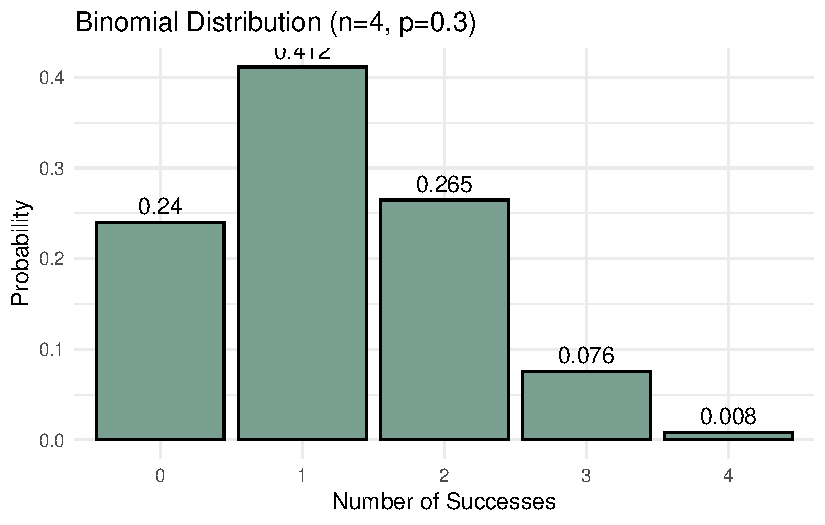
\includegraphics[keepaspectratio]{module4_files/figure-pdf/unnamed-chunk-27-1.pdf}}

\begin{Shaded}
\begin{Highlighting}[]
\DocumentationTok{\#\# dbinom (X=x) given size at 4 and p=.3 P(X=0) = 0.2401}
\FunctionTok{dbinom}\NormalTok{(}\DecValTok{0}\NormalTok{, }\DecValTok{4}\NormalTok{, }\FloatTok{0.3}\NormalTok{)}
\end{Highlighting}
\end{Shaded}

\begin{verbatim}
[1] 0.2401
\end{verbatim}

\begin{Shaded}
\begin{Highlighting}[]
\CommentTok{\# P(X=1) = 0.4116}
\FunctionTok{dbinom}\NormalTok{(}\DecValTok{1}\NormalTok{, }\DecValTok{4}\NormalTok{, }\FloatTok{0.3}\NormalTok{)}
\end{Highlighting}
\end{Shaded}

\begin{verbatim}
[1] 0.4116
\end{verbatim}

\begin{Shaded}
\begin{Highlighting}[]
\CommentTok{\# P(X=2) = 0.2646}
\FunctionTok{dbinom}\NormalTok{(}\DecValTok{2}\NormalTok{, }\DecValTok{4}\NormalTok{, }\FloatTok{0.3}\NormalTok{)}
\end{Highlighting}
\end{Shaded}

\begin{verbatim}
[1] 0.2646
\end{verbatim}

\begin{Shaded}
\begin{Highlighting}[]
\CommentTok{\# P(X=3) = 0.0756}
\FunctionTok{dbinom}\NormalTok{(}\DecValTok{3}\NormalTok{, }\DecValTok{4}\NormalTok{, }\FloatTok{0.3}\NormalTok{)}
\end{Highlighting}
\end{Shaded}

\begin{verbatim}
[1] 0.0756
\end{verbatim}

\begin{Shaded}
\begin{Highlighting}[]
\CommentTok{\# P(X=4) = 0.0081}
\FunctionTok{dbinom}\NormalTok{(}\DecValTok{4}\NormalTok{, }\DecValTok{4}\NormalTok{, }\FloatTok{0.3}\NormalTok{)}
\end{Highlighting}
\end{Shaded}

\begin{verbatim}
[1] 0.0081
\end{verbatim}

\begin{itemize}
\tightlist
\item
  Calculate the probability when the value is less than or equal to 2.
  All calculations below give same answer.
\item
  To confirm accuracy, sum the individual probabilities you calculated
  using dbinom() above. This total should match the value obtained using
  the pbinom() function in R, which gives the cumulative probability up
  to a specified number of successes.
\item
  Less than or equal to is the default state of the function in which we
  use the exact number given.
\end{itemize}

\begin{Shaded}
\begin{Highlighting}[]
\DocumentationTok{\#\#\# P(X\textless{}=2) =0.9163}
\FunctionTok{pbinom}\NormalTok{(}\DecValTok{2}\NormalTok{, }\DecValTok{4}\NormalTok{, }\FloatTok{0.3}\NormalTok{)}
\end{Highlighting}
\end{Shaded}

\begin{verbatim}
[1] 0.9163
\end{verbatim}

\begin{Shaded}
\begin{Highlighting}[]
\FunctionTok{dbinom}\NormalTok{(}\DecValTok{0}\NormalTok{, }\DecValTok{4}\NormalTok{, }\FloatTok{0.3}\NormalTok{) }\SpecialCharTok{+} \FunctionTok{dbinom}\NormalTok{(}\DecValTok{1}\NormalTok{, }\DecValTok{4}\NormalTok{, }\FloatTok{0.3}\NormalTok{) }\SpecialCharTok{+} \FunctionTok{dbinom}\NormalTok{(}\DecValTok{2}\NormalTok{, }\DecValTok{4}\NormalTok{, }\FloatTok{0.3}\NormalTok{)}
\end{Highlighting}
\end{Shaded}

\begin{verbatim}
[1] 0.9163
\end{verbatim}

\begin{Shaded}
\begin{Highlighting}[]
\FloatTok{0.2401} \SpecialCharTok{+} \FloatTok{0.4116} \SpecialCharTok{+} \FloatTok{0.2646}
\end{Highlighting}
\end{Shaded}

\begin{verbatim}
[1] 0.9163
\end{verbatim}

\begin{itemize}
\tightlist
\item
  Calculate the probability when the value is less than 2. All
  calculations below give same answer.
\item
  To calculate less than instead of less than or equal to, we go down 1
  unit (or 1 integer) in our pbinom() function, i.e., using 1 instead of
  2.
\end{itemize}

\begin{Shaded}
\begin{Highlighting}[]
\DocumentationTok{\#\# P(X\textless{}2) = 0.6517}
\FunctionTok{pbinom}\NormalTok{(}\DecValTok{1}\NormalTok{, }\DecValTok{4}\NormalTok{, }\FloatTok{0.3}\NormalTok{)}
\end{Highlighting}
\end{Shaded}

\begin{verbatim}
[1] 0.6517
\end{verbatim}

\begin{Shaded}
\begin{Highlighting}[]
\FunctionTok{dbinom}\NormalTok{(}\DecValTok{0}\NormalTok{, }\DecValTok{4}\NormalTok{, }\FloatTok{0.3}\NormalTok{) }\SpecialCharTok{+} \FunctionTok{dbinom}\NormalTok{(}\DecValTok{1}\NormalTok{, }\DecValTok{4}\NormalTok{, }\FloatTok{0.3}\NormalTok{)}
\end{Highlighting}
\end{Shaded}

\begin{verbatim}
[1] 0.6517
\end{verbatim}

\begin{Shaded}
\begin{Highlighting}[]
\FloatTok{0.2401} \SpecialCharTok{+} \FloatTok{0.4116}
\end{Highlighting}
\end{Shaded}

\begin{verbatim}
[1] 0.6517
\end{verbatim}

\begin{itemize}
\tightlist
\item
  Calculate the probability when the value is greater than 2. All
  calculations below give same answer.
\item
  We use 2 inside the function because greater than is the opposite tail
  to less than or equal to. This means that the numbers should be the
  same as the numbers in a less than or equal to problem, but we need to
  include the lower.tail parameter at False.
\end{itemize}

\begin{Shaded}
\begin{Highlighting}[]
\DocumentationTok{\#\# P(X\textgreater{}2) = 0.0837}
\DecValTok{1} \SpecialCharTok{{-}} \FunctionTok{pbinom}\NormalTok{(}\DecValTok{2}\NormalTok{, }\DecValTok{4}\NormalTok{, }\FloatTok{0.3}\NormalTok{)}
\end{Highlighting}
\end{Shaded}

\begin{verbatim}
[1] 0.0837
\end{verbatim}

\begin{Shaded}
\begin{Highlighting}[]
\FunctionTok{pbinom}\NormalTok{(}\DecValTok{2}\NormalTok{, }\DecValTok{4}\NormalTok{, }\FloatTok{0.3}\NormalTok{, }\AttributeTok{lower.tail =}\NormalTok{ F)}
\end{Highlighting}
\end{Shaded}

\begin{verbatim}
[1] 0.0837
\end{verbatim}

\begin{Shaded}
\begin{Highlighting}[]
\FunctionTok{dbinom}\NormalTok{(}\DecValTok{3}\NormalTok{, }\DecValTok{4}\NormalTok{, }\FloatTok{0.3}\NormalTok{) }\SpecialCharTok{+} \FunctionTok{dbinom}\NormalTok{(}\DecValTok{4}\NormalTok{, }\DecValTok{4}\NormalTok{, }\FloatTok{0.3}\NormalTok{)}
\end{Highlighting}
\end{Shaded}

\begin{verbatim}
[1] 0.0837
\end{verbatim}

\begin{Shaded}
\begin{Highlighting}[]
\FloatTok{0.0756} \SpecialCharTok{+} \FloatTok{0.0081}
\end{Highlighting}
\end{Shaded}

\begin{verbatim}
[1] 0.0837
\end{verbatim}

\begin{itemize}
\tightlist
\item
  Calculate the probability when the value is greater than or equal to
  2.
\item
  We use 1 inside the function because greater than or equal to is the
  opposite tail to less than. This means that the numbers should be the
  same as the numbers in a less than problem, but we need to include the
  lower.tail parameter at False.
\end{itemize}

\begin{Shaded}
\begin{Highlighting}[]
\DocumentationTok{\#\# P(X\textgreater{}=2) = 0.3483}
\DecValTok{1} \SpecialCharTok{{-}} \FunctionTok{pbinom}\NormalTok{(}\DecValTok{1}\NormalTok{, }\DecValTok{4}\NormalTok{, }\FloatTok{0.3}\NormalTok{)}
\end{Highlighting}
\end{Shaded}

\begin{verbatim}
[1] 0.3483
\end{verbatim}

\begin{Shaded}
\begin{Highlighting}[]
\FunctionTok{pbinom}\NormalTok{(}\DecValTok{1}\NormalTok{, }\DecValTok{4}\NormalTok{, }\FloatTok{0.3}\NormalTok{, }\AttributeTok{lower.tail =} \ConstantTok{FALSE}\NormalTok{)}
\end{Highlighting}
\end{Shaded}

\begin{verbatim}
[1] 0.3483
\end{verbatim}

\begin{Shaded}
\begin{Highlighting}[]
\FunctionTok{dbinom}\NormalTok{(}\DecValTok{2}\NormalTok{, }\DecValTok{4}\NormalTok{, }\FloatTok{0.3}\NormalTok{) }\SpecialCharTok{+} \FunctionTok{dbinom}\NormalTok{(}\DecValTok{3}\NormalTok{, }\DecValTok{4}\NormalTok{, }\FloatTok{0.3}\NormalTok{) }\SpecialCharTok{+} \FunctionTok{dbinom}\NormalTok{(}\DecValTok{4}\NormalTok{, }\DecValTok{4}\NormalTok{, }\FloatTok{0.3}\NormalTok{)}
\end{Highlighting}
\end{Shaded}

\begin{verbatim}
[1] 0.3483
\end{verbatim}

\begin{Shaded}
\begin{Highlighting}[]
\FloatTok{0.2646} \SpecialCharTok{+} \FloatTok{0.0756} \SpecialCharTok{+} \FloatTok{0.0081}
\end{Highlighting}
\end{Shaded}

\begin{verbatim}
[1] 0.3483
\end{verbatim}

\bookmarksetup{startatroot}

\chapter{The Continuous Distribution}\label{the-continuous-distribution}

\begin{itemize}
\tightlist
\item
  Properties of a Continuous Random Variable

  \begin{itemize}
  \tightlist
  \item
    The random variable is characterized by (infinitely) uncountable
    values within any interval.
  \item
    Because of the definition \emph{infinite uncountable}, When
    computing probabilities for a continuous random variable,
    \(P(X=x)=0\)
  \item
    Therefore, we cannot assign a nonzero probability to each infinitely
    uncountable value and still have the probabilities sum to one.
  \item
    Thus, \(P(X=a)\) and \(P(X=b)\) both equal zero, and the following
    holds for continuous random variables:
    \(P(a <= X <= b) = P(a < X < b) = P(a <= X < b) = P(a < X <= b)\).
  \end{itemize}
\item
  This is important to consider and compare to discrete probability.
\end{itemize}

\section{Density Functions for Continuous
Distributions}\label{density-functions-for-continuous-distributions}

\subsection{Probability Density
Function}\label{probability-density-function}

\begin{itemize}
\tightlist
\item
  The Probability Density Function is used to describe continuous random
  variables.
\item
  Probability Density Function \(f(x)\) of a continuous random variable
  X describes the relative likelihood that \(X\) assumes a value within
  a given interval (e.g., \(P(a<=X<=b)\), where \(f(x)>=0\) for all
  possible values of \(X\) and the area under \(f(x)\) over all values
  of \(x\) equals one.
\end{itemize}

\subsection{Cumulative Density
Function}\label{cumulative-density-function}

\begin{itemize}
\item
  The Cumulative Density Function \(F(x)\) of a continuous random
  variable X suggests that for any value x of the random variable X, the
  cumulative distribution function \(F(x)\) is computed as,
  \(F(x) = P(X <= x)\) as a result, \(P(a<=X<=b) = F(b)- F(a)\).
\item
  The goal of cumulative distributions is to find the area under the
  curve. The pnorm() function computes the probability at point q to
  find the area under the curve.

  \begin{itemize}
  \tightlist
  \item
    Three arguments of the pnorm() command:
  \end{itemize}

  \begin{enumerate}
  \def\labelenumi{\arabic{enumi}.}
  \tightlist
  \item
    q is the value of interest;
  \item
    The mean (mean);
  \item
    The standard deviation (sd);
  \end{enumerate}
\item
  Also an optional lower.tail parameter, which is defaulted to TRUE
  signifying \textless{} or \textless=.
\item
  We can also work backwards to find a value given a probability. The
  qnorm() function computes the quantile value at p to find the value
  associated with a probability.

  \begin{itemize}
  \tightlist
  \item
    Three arguments of the qnorm() command:
  \end{itemize}

  \begin{enumerate}
  \def\labelenumi{\arabic{enumi}.}
  \tightlist
  \item
    p is the cumulative probability;
  \item
    The mean (mean);
  \item
    The standard deviation (sd);
  \end{enumerate}
\item
  Also an optional lower.tail parameter, which is defaulted to TRUE
  signifying \textless{} or \textless=.
\end{itemize}

\section{The Normal Distribution}\label{the-normal-distribution}

\begin{itemize}
\item
  The normal distribution serves as the cornerstone of statistical
  inference.
\item
  Data is symmetric about its mean.
\item
  Mean=Median=Mode.
\item
  The distribution is bell-shaped.
\item
  The distribution is asymptotic, which means that the tails get closer
  and closer to the horizontal axis, but never touch it.
\item
  Closely approximates the probability distribution of a wide range of
  random variables, such as the following:

  \begin{itemize}
  \tightlist
  \item
    Heights and weights of newborn babies.
  \item
    Scores on SAT.
  \item
    Cumulative debt of college graduates.
  \end{itemize}
\item
  The normal distribution is completely described by two parameters:
  population mean \(\mu\), which describes the central location of the
  distribution,and population variance \(\sigma^2\), which describes the
  dispersion of the distribution.
\end{itemize}

\begin{figure}[H]

{\centering \pandocbounded{\includegraphics[keepaspectratio]{Pictures/Ch4/NormalDist.png}}

}

\caption{Normal Distribution}

\end{figure}%

\begin{itemize}
\tightlist
\item
  A special case of the normal distribution:

  \begin{itemize}
  \tightlist
  \item
    Mean is equal to zero (E(Z) = 0).
  \item
    Standard deviation is equal to one (SD(Z) = 1).
  \end{itemize}
\end{itemize}

\begin{Shaded}
\begin{Highlighting}[]
\CommentTok{\# Solving the figure above using the pnorm() command in R.  P(Z\textless{}=0)}
\FunctionTok{pnorm}\NormalTok{(}\AttributeTok{q =} \DecValTok{0}\NormalTok{, }\AttributeTok{mean =} \DecValTok{0}\NormalTok{, }\AttributeTok{sd =} \DecValTok{1}\NormalTok{)}
\end{Highlighting}
\end{Shaded}

\begin{verbatim}
[1] 0.5
\end{verbatim}

\begin{Shaded}
\begin{Highlighting}[]
\CommentTok{\# Or the following because the default value of the mean and sd are 0}
\CommentTok{\# and 1.}
\FunctionTok{pnorm}\NormalTok{(}\DecValTok{0}\NormalTok{)}
\end{Highlighting}
\end{Shaded}

\begin{verbatim}
[1] 0.5
\end{verbatim}

\begin{itemize}
\item
  If we assume a mean of 0 and a standard deviation of 1, and we are
  looking for the probability when the mean is 0, we will get a .5
  probability or 50 percent (.5*100). This is because the curve is
  normal with identical sides.
\item
  We can also solve this backwards. Below is the qnorm() command, which
  solves the figure above looking at probability instead of values.
\end{itemize}

\begin{Shaded}
\begin{Highlighting}[]
\CommentTok{\# P(Z \textgreater{}= z) = .5}
\FunctionTok{qnorm}\NormalTok{(}\FloatTok{0.5}\NormalTok{, }\DecValTok{0}\NormalTok{, }\DecValTok{1}\NormalTok{)}
\end{Highlighting}
\end{Shaded}

\begin{verbatim}
[1] 0
\end{verbatim}

\begin{Shaded}
\begin{Highlighting}[]
\CommentTok{\# Or}
\FunctionTok{qnorm}\NormalTok{(}\FloatTok{0.5}\NormalTok{)}
\end{Highlighting}
\end{Shaded}

\begin{verbatim}
[1] 0
\end{verbatim}

\section{Empirical Rule}\label{empirical-rule}

\begin{itemize}
\item
  Chevyshev's Theorem states that at least \(1 - 1/z^2\)\% of the data
  lies between \(z\) standard deviations from the mean. This result does
  not depend on the shape of the distribution.
\item
  With a normal distribution, we can assume approximately the following
  under the empirical rule:

  \begin{itemize}
  \tightlist
  \item
    68\% of values within one SD of the mean;
  \item
    95\% of values within two SD of the mean;
  \item
    99.7\% of values within three SD of the mean.
  \end{itemize}
\end{itemize}

\begin{figure}[H]

{\centering \pandocbounded{\includegraphics[keepaspectratio]{Pictures/Ch4/EmpiricalRule.png}}

}

\caption{Empirical Rule}

\end{figure}%

\section{Calculating z-scores}\label{calculating-z-scores}

\begin{itemize}
\item
  A z-score allows description and comparison of where an observation
  falls compared to the other observations for a normally distributed
  variable.
\item
  A z-score is calculated as the number of standard deviations an
  observation is away from the mean.
\item
  A normally distributed variable can be used to create z-scores.
\item
  Purpose: This formula calculates the z-score of an individual data
  point.
\item
  Interpretation: It tells us how many standard deviations a specific
  value \(x\) is from the mean of the dataset.
\item
  The \(x_i\) represents the value of variable \(x\) for a single
  observation, \(\mu_x\) is the mean of the \(x\) variable, \(\sigma_x\)
  is the standard deviation of the \(x\) variable. So, \(z_i\) is the
  difference between the observation value and the mean value for a
  variable and is converted by the denominator into standard deviations.
  The final z-score for an observation is the number of standard
  deviations it is from the mean. \[z_i = (x_i - \mu_x)/\sigma_x\].
\item
  A z score or z value specifies by how many standard deviations the
  corresponding x value falls above (z \textgreater{} 0) or below (z
  \textless{} 0) the mean.

  \begin{itemize}
  \tightlist
  \item
    A positive z indicates by how many standard deviations the
    corresponding x lies above mean.
  \item
    A zero z indicates that the corresponding x equals mean.
  \item
    A negative z indicates by how many standard deviations the
    corresponding x lies below mean.
  \end{itemize}
\item
  Example of a z-score calculation: Scores on a management aptitude exam
  are normally distributed with a mean of 72 and a standard deviation of
  8.

  \begin{itemize}
  \tightlist
  \item
    What is the probability that a randomly selected manager will score
    above 60?
  \item
    First, we could transform the random variable X to Z score using the
    transformation formula:
  \end{itemize}
\end{itemize}

\begin{Shaded}
\begin{Highlighting}[]
\NormalTok{(}\DecValTok{60} \SpecialCharTok{{-}} \DecValTok{72}\NormalTok{)}\SpecialCharTok{/}\DecValTok{8}
\end{Highlighting}
\end{Shaded}

\begin{verbatim}
[1] -1.5
\end{verbatim}

\begin{itemize}
\tightlist
\item
  Then, you can calculate the probability using the standard normal
  distribution, which has a mean of 0 and a standard deviation of 1.
\end{itemize}

\begin{Shaded}
\begin{Highlighting}[]
\CommentTok{\# P(Z \textgreater{} {-}1.5)}
\FunctionTok{pnorm}\NormalTok{(}\SpecialCharTok{{-}}\FloatTok{1.5}\NormalTok{, }\DecValTok{0}\NormalTok{, }\DecValTok{1}\NormalTok{, }\AttributeTok{lower.tail =} \ConstantTok{FALSE}\NormalTok{)}
\end{Highlighting}
\end{Shaded}

\begin{verbatim}
[1] 0.9331928
\end{verbatim}

\begin{Shaded}
\begin{Highlighting}[]
\CommentTok{\# Or similarly, we could use the line below because of the default}
\CommentTok{\# values associated with the pnorm() command}
\FunctionTok{pnorm}\NormalTok{(}\SpecialCharTok{{-}}\FloatTok{1.5}\NormalTok{, }\AttributeTok{lower.tail =} \ConstantTok{FALSE}\NormalTok{)}
\end{Highlighting}
\end{Shaded}

\begin{verbatim}
[1] 0.9331928
\end{verbatim}

\begin{itemize}
\tightlist
\item
  Also, because R handles the standard normal transformation on our
  behalf with its inclusion of parameters, we can use the pnorm()
  command with the mean and standard deviation provided above to
  calculate the probability in less steps.
\end{itemize}

\begin{Shaded}
\begin{Highlighting}[]
\CommentTok{\# Note the same answer as above.  P(X \textgreater{} 60)}
\FunctionTok{pnorm}\NormalTok{(}\DecValTok{60}\NormalTok{, }\DecValTok{72}\NormalTok{, }\DecValTok{8}\NormalTok{, }\AttributeTok{lower.tail =} \ConstantTok{FALSE}\NormalTok{)}
\end{Highlighting}
\end{Shaded}

\begin{verbatim}
[1] 0.9331928
\end{verbatim}

\begin{itemize}
\item
  To answer the question, there is a 0.933 probability or a 93.3\%
  chance that a randomly selected manager will score above a 60 on the
  managerial aptitude exam.
\item
  In order to get the percentage in R, we simply multiply the answer by
  100.
\end{itemize}

\begin{Shaded}
\begin{Highlighting}[]
\FunctionTok{pnorm}\NormalTok{(}\DecValTok{60}\NormalTok{, }\DecValTok{72}\NormalTok{, }\DecValTok{8}\NormalTok{, }\AttributeTok{lower.tail =} \ConstantTok{FALSE}\NormalTok{) }\SpecialCharTok{*} \DecValTok{100}
\end{Highlighting}
\end{Shaded}

\begin{verbatim}
[1] 93.31928
\end{verbatim}

\section{Finding Utility in Calculating
Probability}\label{finding-utility-in-calculating-probability}

\begin{itemize}
\tightlist
\item
  Example using pnorm() with Word Problems: Suppose the life of a
  particular brand of laptop battery is normally distributed with a mean
  of 6 hours and a standard deviation of 0.9 hours. Use R to calculate
  the probability that the battery will last more than 8 hours before
  running out of power and document that probability below.
\end{itemize}

\begin{Shaded}
\begin{Highlighting}[]
\CommentTok{\# P(X \textgreater{} 8)}
\FunctionTok{pnorm}\NormalTok{(}\DecValTok{8}\NormalTok{, }\DecValTok{6}\NormalTok{, }\FloatTok{0.9}\NormalTok{, }\AttributeTok{lower.tail =} \ConstantTok{FALSE}\NormalTok{)}
\end{Highlighting}
\end{Shaded}

\begin{verbatim}
[1] 0.01313415
\end{verbatim}

\begin{itemize}
\tightlist
\item
  The time for a professor to grade a student's homework in business
  statistics is normally distributed with a mean of 15 minutes and a
  standard deviation of 3.5 minutes. What is the probability that
  randomly selected homework will require less than 16 minutes to grade?
\end{itemize}

\begin{Shaded}
\begin{Highlighting}[]
\CommentTok{\# P(X \textless{} 16)}
\FunctionTok{pnorm}\NormalTok{(}\DecValTok{16}\NormalTok{, }\DecValTok{15}\NormalTok{, }\FloatTok{3.5}\NormalTok{)}
\end{Highlighting}
\end{Shaded}

\begin{verbatim}
[1] 0.6124515
\end{verbatim}

\begin{itemize}
\tightlist
\item
  What percentage of randomly selected homeworks will require less than
  16 minutes to grade?
\end{itemize}

\begin{Shaded}
\begin{Highlighting}[]
\FunctionTok{pnorm}\NormalTok{(}\DecValTok{16}\NormalTok{, }\DecValTok{15}\NormalTok{, }\FloatTok{3.5}\NormalTok{) }\SpecialCharTok{*} \DecValTok{100}
\end{Highlighting}
\end{Shaded}

\begin{verbatim}
[1] 61.24515
\end{verbatim}

\section{Finding Probability Between Two
Values}\label{finding-probability-between-two-values}

\begin{itemize}
\tightlist
\item
  We mentioned above that in order to find probability between 2 values
  a and b, we could use the following equation:
  \(P(a<=X<=b) = F(b)- F(a)\).
\item
  To use this formula, find P(−1.52 \textless= Z \textless= 1.96). This
  would equal P(Z\textless=1.96)−P(Z\textless=−1.52) given a standard
  normal random variable Z we get the commands below.
\end{itemize}

\begin{Shaded}
\begin{Highlighting}[]
\CommentTok{\# P(Z \textless{}= 1.96) {-} P(Z \textless{}= {-}1.52)}
\FunctionTok{pnorm}\NormalTok{(}\FloatTok{1.96}\NormalTok{, }\DecValTok{0}\NormalTok{, }\DecValTok{1}\NormalTok{) }\SpecialCharTok{{-}} \FunctionTok{pnorm}\NormalTok{(}\SpecialCharTok{{-}}\FloatTok{1.52}\NormalTok{, }\DecValTok{0}\NormalTok{, }\DecValTok{1}\NormalTok{)}
\end{Highlighting}
\end{Shaded}

\begin{verbatim}
[1] 0.9107466
\end{verbatim}

\section{Finding Value Given a
Probability}\label{finding-value-given-a-probability}

\begin{itemize}
\tightlist
\item
  We use R's pnorm() and qnorm() commands to solve problems associated
  with the normal distribution.
\item
  If we want to find a particular x value for a given cumulative
  probability (p), then we enter ``qnorm(p, μ, σ)''.
\end{itemize}

\begin{Shaded}
\begin{Highlighting}[]
\CommentTok{\# P(X \textgreater{} x) = 0.10}
\FunctionTok{qnorm}\NormalTok{(}\FloatTok{0.9}\NormalTok{, }\FloatTok{7.49}\NormalTok{, }\FloatTok{6.41}\NormalTok{)}
\end{Highlighting}
\end{Shaded}

\begin{verbatim}
[1] 15.70475
\end{verbatim}

\begin{Shaded}
\begin{Highlighting}[]
\CommentTok{\# or}
\FunctionTok{qnorm}\NormalTok{(}\FloatTok{0.1}\NormalTok{, }\FloatTok{7.49}\NormalTok{, }\FloatTok{6.41}\NormalTok{, }\AttributeTok{lower.tail =} \ConstantTok{FALSE}\NormalTok{)}
\end{Highlighting}
\end{Shaded}

\begin{verbatim}
[1] 15.70475
\end{verbatim}

\section{Finding Utility in Calculating Values from
Probability}\label{finding-utility-in-calculating-values-from-probability}

\begin{itemize}
\tightlist
\item
  Example of qnorm() with Word Problems: The stock price of a particular
  asset has a mean and standard deviation of \$58.50 and \$8.25,
  respectively. What is the 95th percentile of this stock price?
\end{itemize}

\begin{Shaded}
\begin{Highlighting}[]
\CommentTok{\# P(X\textless{}=x) =.95}
\FunctionTok{qnorm}\NormalTok{(}\FloatTok{0.95}\NormalTok{, }\FloatTok{58.5}\NormalTok{, }\FloatTok{8.25}\NormalTok{)}
\end{Highlighting}
\end{Shaded}

\begin{verbatim}
[1] 72.07004
\end{verbatim}

\begin{itemize}
\tightlist
\item
  The salary of teachers in a particular school district is normally
  distributed with a mean of \$50,000 and a standard deviation of
  \$2,500. Due to budget limitations, it has been decided that the
  teachers who are in the top 2.5\% of the salaries would not get a
  raise. What is the salary level that divides the teachers into one
  group that gets a raise and one that does not?
\end{itemize}

\begin{Shaded}
\begin{Highlighting}[]
\CommentTok{\# P(X\textgreater{}=x) =.025}
\FunctionTok{qnorm}\NormalTok{(}\FloatTok{0.025}\NormalTok{, }\DecValTok{50000}\NormalTok{, }\DecValTok{2500}\NormalTok{, }\AttributeTok{lower.tail =} \ConstantTok{FALSE}\NormalTok{)}
\end{Highlighting}
\end{Shaded}

\begin{verbatim}
[1] 54899.91
\end{verbatim}

\begin{itemize}
\tightlist
\item
  You are planning a May camping trip to a National Park in Alaska and
  want to make sure your sleeping bag is warm enough. The average low
  temperature in the park for May follows a normal distribution with a
  mean of 32°F and a standard deviation of 8°F. Above what temperature
  must the sleeping bag be suited such that the temperature will be too
  cold only 5\% of the time?
\end{itemize}

\begin{Shaded}
\begin{Highlighting}[]
\CommentTok{\# P(X\textless{}=x) =.05}
\FunctionTok{qnorm}\NormalTok{(}\FloatTok{0.05}\NormalTok{, }\DecValTok{32}\NormalTok{, }\DecValTok{8}\NormalTok{)}
\end{Highlighting}
\end{Shaded}

\begin{verbatim}
[1] 18.84117
\end{verbatim}

\section{Central Limit Theorem (CLT)}\label{central-limit-theorem-clt}

\begin{itemize}
\item
  The Central Limit Theorem (CLT) is one of the most important concepts
  in statistics because it allows us to use the normal distribution to
  make inferences about populations --- even when the underlying data is
  not normally distributed. In other words, as long as our sample is
  large enough (generally n ≥ 30), we can assume that the distribution
  of sample means will be approximately normal, regardless of the shape
  of the original data.
\item
  CLT refers to the fact that, in many situations, when independent
  random variables are summed up, their properly normalized sum tends
  toward a normal distribution even if the original variables themselves
  are not normally distributed. Therefore, CLT suggests that for any
  population X with expected value \(\mu\) and standard deviation
  \(\sigma\) the sampling distribution of \(X\) will be approximately
  normal if the sample size \(n\) is sufficiently large.
\item
  The CLT tells us that, regardless of the original distribution of a
  population, the sampling distribution of the sample mean approaches a
  normal distribution as the sample size gets larger. We use the CLT
  when we want to estimate population parameters (like the mean) from
  sample data and apply techniques that rely on normality, such as
  confidence intervals and hypothesis testing. This allows us to make
  inferences about the population using the normal distribution even
  when the population itself isn't normally distributed.
\item
  The Central Limit Theorem (CLT) holds true for continuous variables,
  regardless of whether they are normally distributed or not. Generally,
  the normal distribution approximation is justified when the sample
  size is sufficiently large, typically \(n≥30\). If the sample means
  are approximately normal, we can transform them into a standard normal
  form. The standard deviation of the sample means (also called the
  standard error) can be estimated using the population standard
  deviation and the sample size that makes up the distribution.
\item
  If \(\bar{X}\) is approximately normal, then we can transform it using
  an updated formula of the z-score formula with standard error
  \(𝑍=(𝑋- \mu)/(\sigma/\sqrt(n))\)
\item
  Next, we want to create an experiment where we simulate why the CLT
  holds true. The rnorm() command pulls random data from a normal
  distribution. However, even when the sample is small, it can appear
  not normal - even though it is from a normal distribution.
\end{itemize}

\begin{Shaded}
\begin{Highlighting}[]
\FunctionTok{set.seed}\NormalTok{(}\DecValTok{1}\NormalTok{)}
\CommentTok{\# Sample of n = 10}
\FunctionTok{hist}\NormalTok{(}\FunctionTok{rnorm}\NormalTok{(}\DecValTok{10}\NormalTok{), }\AttributeTok{xlim =} \FunctionTok{c}\NormalTok{(}\SpecialCharTok{{-}}\DecValTok{3}\NormalTok{, }\DecValTok{3}\NormalTok{))}
\end{Highlighting}
\end{Shaded}

\pandocbounded{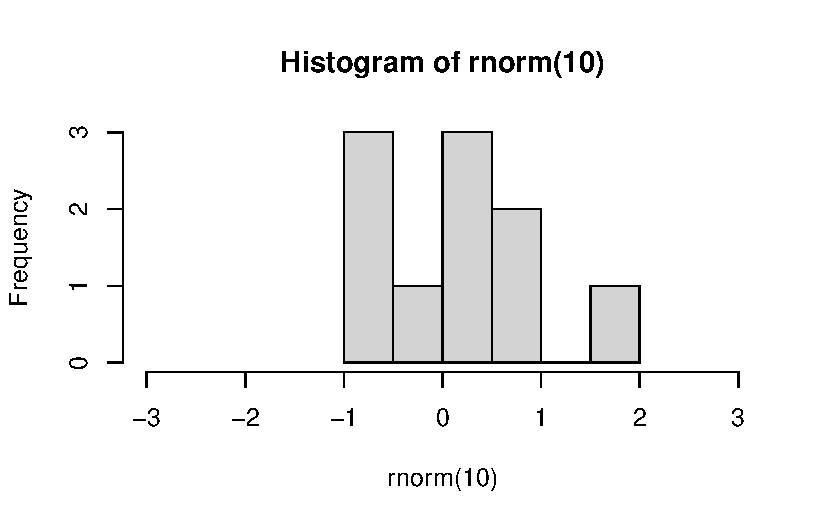
\includegraphics[keepaspectratio]{module4_files/figure-pdf/unnamed-chunk-47-1.pdf}}

\begin{itemize}
\tightlist
\item
  If we increase the sample size, we should all see a nice normal bell
  shape distribution like the one below.
\end{itemize}

\begin{Shaded}
\begin{Highlighting}[]
\FunctionTok{set.seed}\NormalTok{(}\DecValTok{1}\NormalTok{)}
\CommentTok{\# Sample of n = 1000}
\FunctionTok{hist}\NormalTok{(}\FunctionTok{rnorm}\NormalTok{(}\DecValTok{1000}\NormalTok{), }\AttributeTok{xlim =} \FunctionTok{c}\NormalTok{(}\SpecialCharTok{{-}}\DecValTok{3}\NormalTok{, }\DecValTok{3}\NormalTok{))}
\end{Highlighting}
\end{Shaded}

\pandocbounded{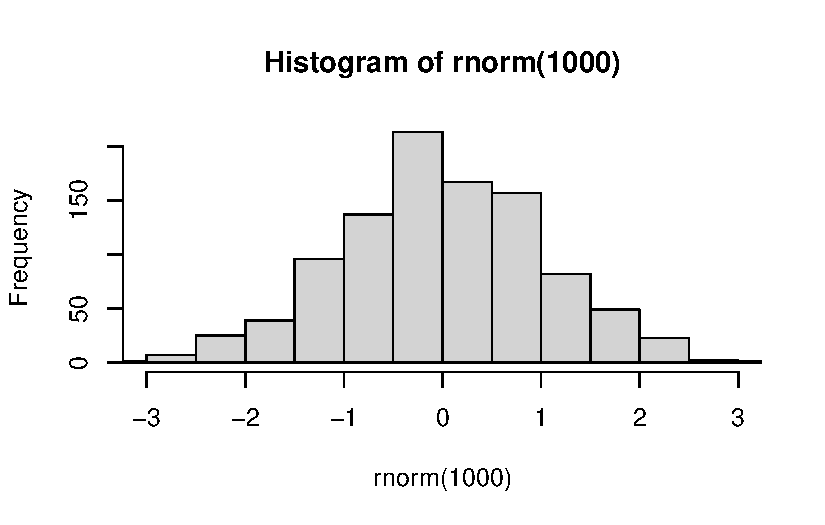
\includegraphics[keepaspectratio]{module4_files/figure-pdf/unnamed-chunk-48-1.pdf}}

\begin{itemize}
\item
  The x limits are set from -3 to 3 because a normal distribution
  follows the empirical rule discussed above (almost all data is within
  3 sd of the mean).
\item
  Relating this to the CLT, the CLT states that the sum or mean of a
  large number of independent observations from the same underlying
  distribution has an approximate normal distribution. If we were to
  take a 6 sided dice, in any given roll, we would expect the average.
  This means that the expected value E(X) will be the mean as discussed
  above.
\end{itemize}

\begin{Shaded}
\begin{Highlighting}[]
\CommentTok{\# Creating a sample}
\NormalTok{d }\OtherTok{\textless{}{-}} \DecValTok{1}\SpecialCharTok{:}\DecValTok{6}
\CommentTok{\# Calculating the expected value E(X) which equals the population}
\CommentTok{\# mean}
\FunctionTok{mean}\NormalTok{(d)  }\CommentTok{\#3.5}
\end{Highlighting}
\end{Shaded}

\begin{verbatim}
[1] 3.5
\end{verbatim}

\begin{itemize}
\tightlist
\item
  Rolling a dice only one time would not give us enough data to assume a
  normal distribution under the CLT. However, if we were to roll a
  higher number of times, and repeat that experiment \(n\) number of
  times, we would expect that as \(n\) grows, we would approach a normal
  distribution.
\end{itemize}

\begin{Shaded}
\begin{Highlighting}[]
\CommentTok{\# First, let\textquotesingle{}s roll the dice 1000 times.  We would expect the average}
\CommentTok{\# like shown below.}
\FunctionTok{set.seed}\NormalTok{(}\DecValTok{1}\NormalTok{)}
\NormalTok{NumberofRolls }\OtherTok{\textless{}{-}} \DecValTok{1000}
\NormalTok{x }\OtherTok{\textless{}{-}} \FunctionTok{sample}\NormalTok{(d, NumberofRolls, }\AttributeTok{replace =} \ConstantTok{TRUE}\NormalTok{)}
\CommentTok{\# The mean(x) is 3.514 and our mean of 1 through 6 is 3.5.  We}
\CommentTok{\# estimated about the average.}
\FunctionTok{mean}\NormalTok{(x)}
\end{Highlighting}
\end{Shaded}

\begin{verbatim}
[1] 3.514
\end{verbatim}

\begin{Shaded}
\begin{Highlighting}[]
\FunctionTok{hist}\NormalTok{(x)}
\end{Highlighting}
\end{Shaded}

\pandocbounded{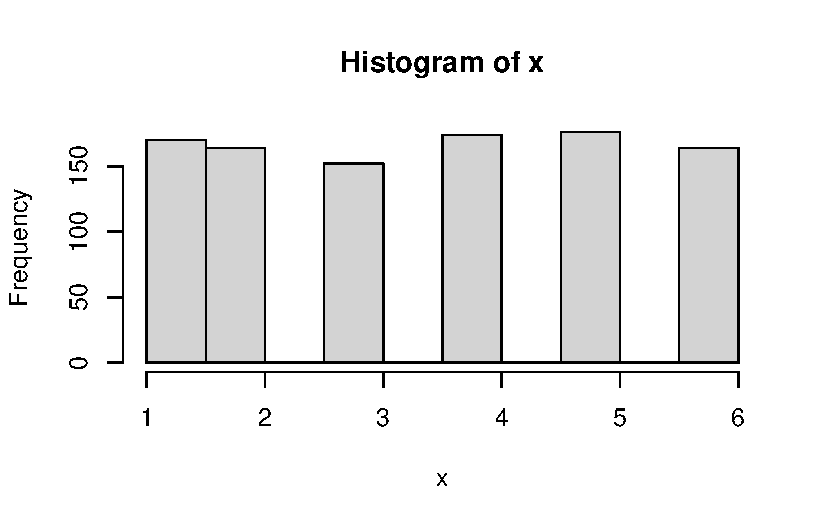
\includegraphics[keepaspectratio]{module4_files/figure-pdf/unnamed-chunk-50-1.pdf}}

\begin{itemize}
\tightlist
\item
  Next, if we repeat the dice roll experiment that we ran 1,000 times
  above, we can see the normal distribution start to take shape. The
  example below has a loop for simulation purposes. This loop rolls x
  with allowed values 1 to 6 - 1,000 times - and then does that 100
  times. The more we do this, the closer we get to approximating the
  mean (3.5) as our histogram starts to get more narrow.
\end{itemize}

\begin{Shaded}
\begin{Highlighting}[]
\FunctionTok{set.seed}\NormalTok{(}\DecValTok{1}\NormalTok{)}
\NormalTok{t }\OtherTok{\textless{}{-}} \DecValTok{0}
\ControlFlowTok{for}\NormalTok{ (i }\ControlFlowTok{in} \DecValTok{1}\SpecialCharTok{:}\DecValTok{100}\NormalTok{) \{}
\NormalTok{    NumberofRolls }\OtherTok{\textless{}{-}} \DecValTok{1000}
\NormalTok{    x }\OtherTok{\textless{}{-}} \FunctionTok{sample}\NormalTok{(d, NumberofRolls, }\AttributeTok{replace =} \ConstantTok{TRUE}\NormalTok{)}
\NormalTok{    t[i] }\OtherTok{\textless{}{-}} \FunctionTok{mean}\NormalTok{(x)}
\NormalTok{\}}
\FunctionTok{hist}\NormalTok{(t, }\AttributeTok{xlim =} \FunctionTok{c}\NormalTok{(}\DecValTok{3}\NormalTok{, }\DecValTok{4}\NormalTok{))}
\end{Highlighting}
\end{Shaded}

\pandocbounded{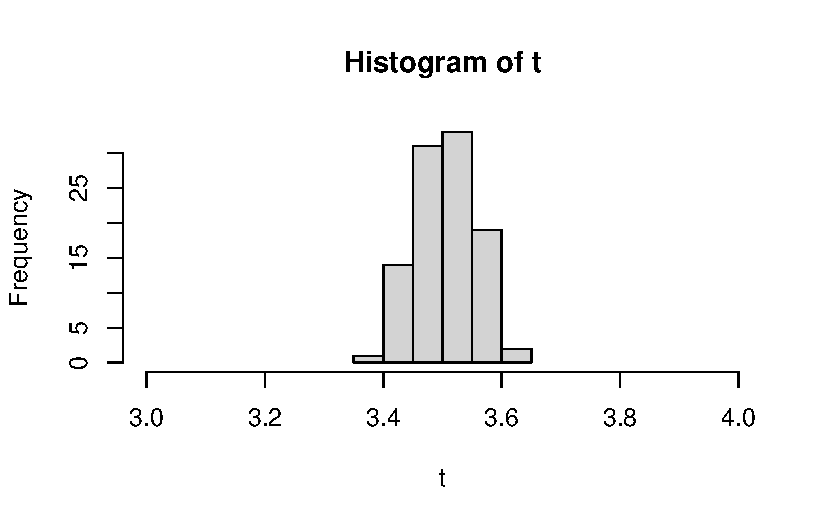
\includegraphics[keepaspectratio]{module4_files/figure-pdf/unnamed-chunk-51-1.pdf}}

\begin{itemize}
\tightlist
\item
  Important to note that for any sample size \(n\), the sampling
  distribution of \(\bar{x}\) is normal if the population X from which
  the sample is drawn is normally distributed, meaning, there is no need
  to use CLT.
\end{itemize}

\section{Standard Error (SE)}\label{standard-error-se}

\begin{itemize}
\item
  The \(SE\) is the standard deviation of the sampling distribution for
  all samples of size \(n\).
\item
  It is unusual to have the entire population for computing the
  population standard deviation, and it is also unusual to have a large
  number of samples from one population. A close approximation to this
  value is called the standard error of the mean. \(SE=sd/\sqrt(n)\).
\item
  Standard Deviation vs.~Standard Error

  \begin{itemize}
  \tightlist
  \item
    SD: Measure of variability in the sample.
  \item
    SE: Estimate of how closely the sample represents the population.
  \end{itemize}
\item
  Purpose: This is the standard error formula used to assess the
  distribution of sample means around the population mean.
\item
  Interpretation: This measures how much the sample mean, \(\bar{X}\) is
  expected to vary from the population mean given the sample size \(n\).
\item
  The standard deviation measures the spread of individual data points,
  while the standard error measures the spread of sample means.
\item
  The standard deviation and standard error are both measures of
  variability but are used in different contexts and serve different
  purposes. The standard deviation quantifies the spread of individual
  data points within a dataset. It is often used when analyzing the
  distribution of a single sample or population. On the other hand, the
  standard error is a measure of the precision of the sample mean in
  estimating the population mean. It tells us how much the sample mean
  is likely to vary from the true population mean if we were to take
  repeated samples. The standard error is derived from the standard
  deviation but is scaled by the square root of the sample size, meaning
  it decreases as the sample size increases. This makes it particularly
  useful in inferential statistics, where it helps assess the accuracy
  of estimates based on sample data.
\item
  Example using SD: Given that \(\mu\) = 16 inches and \(\sigma\) = 0.8
  inches, determine the following: What is the probability that a
  randomly selected pizza is less than 15.5 inches?
\end{itemize}

\begin{Shaded}
\begin{Highlighting}[]
\CommentTok{\# P(X \textless{} 15.5)}
\FunctionTok{pnorm}\NormalTok{(}\FloatTok{15.5}\NormalTok{, }\DecValTok{16}\NormalTok{, }\FloatTok{0.8}\NormalTok{)}
\end{Highlighting}
\end{Shaded}

\begin{verbatim}
[1] 0.2659855
\end{verbatim}

\begin{itemize}
\item
  Example using SE: What is the probability that 2 randomly selected
  pizzas average less than 15.5 inches?

  \begin{itemize}
  \tightlist
  \item
    \(P(\bar{X} < 15.5)\)
  \end{itemize}

\begin{Shaded}
\begin{Highlighting}[]
\FunctionTok{pnorm}\NormalTok{(}\FloatTok{15.5}\NormalTok{, }\DecValTok{16}\NormalTok{, }\FloatTok{0.8}\SpecialCharTok{/}\FunctionTok{sqrt}\NormalTok{(}\DecValTok{2}\NormalTok{))}
\end{Highlighting}
\end{Shaded}

\begin{verbatim}
[1] 0.1883796
\end{verbatim}
\item
  Additional Examples using SE:

  \begin{itemize}
  \tightlist
  \item
    Anne wants to determine if the marketing campaign has had a
    lingering effect on the amount of money customers spend on coffee.
    Before the campaign, \(\mu\) = \$4.18 and \(\sigma\) = \$0.84. Based
    on 50 customers sampled after the campaign, \(\mu\) = \$4.26.
  \item
    \(P(\bar{X} > 4.26)\)
  \end{itemize}

\begin{Shaded}
\begin{Highlighting}[]
\FunctionTok{pnorm}\NormalTok{(}\FloatTok{4.26}\NormalTok{, }\FloatTok{4.18}\NormalTok{, }\FloatTok{0.84}\SpecialCharTok{/}\FunctionTok{sqrt}\NormalTok{(}\DecValTok{50}\NormalTok{), }\AttributeTok{lower.tail =} \ConstantTok{FALSE}\NormalTok{)}
\end{Highlighting}
\end{Shaded}

\begin{verbatim}
[1] 0.2503353
\end{verbatim}

  \begin{itemize}
  \tightlist
  \item
    Over the entire six years that students attend an Ohio elementary
    school, they are absent, on average, 28 days due to influenza.
    Assume that the standard deviation over this time period is
    \(\sigma\) = 9 days. Upon graduation from elementary school, a
    random sample of 36 students is taken and asked how many days of
    school they missed due to influenza. What is the probability that
    the sample mean is between 25 and 30 school days?
  \end{itemize}
\item
  \(P(\bar{X} < 30)-P(\bar{X} < 25)\)
\end{itemize}

\begin{Shaded}
\begin{Highlighting}[]
\FunctionTok{pnorm}\NormalTok{(}\DecValTok{30}\NormalTok{, }\DecValTok{28}\NormalTok{, }\DecValTok{9}\SpecialCharTok{/}\FunctionTok{sqrt}\NormalTok{(}\DecValTok{36}\NormalTok{)) }\SpecialCharTok{{-}} \FunctionTok{pnorm}\NormalTok{(}\DecValTok{25}\NormalTok{, }\DecValTok{28}\NormalTok{, }\DecValTok{9}\SpecialCharTok{/}\FunctionTok{sqrt}\NormalTok{(}\DecValTok{36}\NormalTok{))}
\end{Highlighting}
\end{Shaded}

\begin{verbatim}
[1] 0.8860386
\end{verbatim}

\begin{itemize}
\tightlist
\item
  According to the Bureau of Labor Statistics, it takes an average of 22
  weeks for someone over 55 to find a new job. Assume that the
  probability distribution is normal and that the standard deviation is
  two weeks. What is the probability that eight workers over the age of
  55 take an average of more than 20 weeks to find a job?
\item
  \(P(\bar{X} >20)\)
\end{itemize}

\begin{Shaded}
\begin{Highlighting}[]
\FunctionTok{pnorm}\NormalTok{(}\DecValTok{20}\NormalTok{, }\DecValTok{22}\NormalTok{, }\DecValTok{2}\SpecialCharTok{/}\FunctionTok{sqrt}\NormalTok{(}\DecValTok{8}\NormalTok{), }\AttributeTok{lower.tail =} \ConstantTok{FALSE}\NormalTok{)}
\end{Highlighting}
\end{Shaded}

\begin{verbatim}
[1] 0.9976611
\end{verbatim}

\section{Sampling Distribution of the Sample
Proportion}\label{sampling-distribution-of-the-sample-proportion}

\begin{itemize}
\tightlist
\item
  Estimator Sample proportion \(\bar{P}\) is used to estimate the
  population parameter \(p\).
\item
  Estimate: A particular value of the estimator \(\bar{p}\).
\item
  The expected value of \(\bar{P}=E(\bar{P})=𝑝\).
\item
  The standard deviation of \(\bar{P}\) is referred to as the standard
  error of the sample proportion, which equals
  \(se(\bar{P}) = \sqrt(p*(1-p)/n\).
\item
  Purpose: This formula calculates the z-score for a sample proportion
  \(\hat{P}\) by comparing it to a population proportion, \(P\).
\item
  Interpretation: It measures how far the sample proportion deviates
  from the population proportion in terms of the standard deviation (for
  proportions).
\item
  The Central Limit Theorem for the Sample Proportion.

  \begin{itemize}
  \tightlist
  \item
    For any population proportion \(p\), the sampling \(\bar{P}\) is
    approximately normal if the sample size \(n\) is sufficiently large.
  \item
    As a general guideline, the normal distribution approximation is
    justified when \(n*p>=5\) and \(n((1-p)>=5\).
  \item
    If \(\bar{P}\) is normal, we can transform it into the standard
    normal random variable as \(Z=(\hat{P}-E(\bar{P})/se(\bar{P})\) =
    \((\hat{P}-p)/(\sqrt(p*(1-p)/n))\).
  \item
    Using the pnorm() function, this would translate to the following:
    \(pnorm(\hat{P}, E(\bar{P}), se(\bar{P})\) , where
    \(se(\bar{P}) = \sqrt(p*(1-p)/n)\)
  \end{itemize}
\end{itemize}

\subsection{Examples Using
Proportions}\label{examples-using-proportions}

\begin{itemize}
\tightlist
\item
  Anne wants to determine if the marketing campaign has had a lingering
  effect on the proportion of customers who are women and teenage girls.
  Before the campaign, p = 0.43 for women and p = 0.21 for teenage
  girls. Based on 50 women and 50 teenage girls sampled after the
  campaign, p = 0.46 and p = 0.34, respectively.
\item
  To calculate the probability that the marketing campaign had a
  lingering effect on women, we use \(P(\hat{P} >= .46)\).
\end{itemize}

\begin{Shaded}
\begin{Highlighting}[]
\FunctionTok{pnorm}\NormalTok{(}\FloatTok{0.46}\NormalTok{, }\FloatTok{0.43}\NormalTok{, }\FunctionTok{sqrt}\NormalTok{(}\FloatTok{0.43} \SpecialCharTok{*}\NormalTok{ (}\DecValTok{1} \SpecialCharTok{{-}} \FloatTok{0.43}\NormalTok{)}\SpecialCharTok{/}\DecValTok{50}\NormalTok{), }\AttributeTok{lower.tail =} \ConstantTok{FALSE}\NormalTok{)}
\end{Highlighting}
\end{Shaded}

\begin{verbatim}
[1] 0.3341494
\end{verbatim}

\begin{itemize}
\item
  The probability that the observed proportion is 0.46 or higher,
  assuming the true proportion remains 0.43, is approximately 0.3341.
\item
  To calculate the probability that the marketing campaign had a
  lingering effect on teenage girls, we use \(P(\hat{P} >= .34)\).
\end{itemize}

\begin{Shaded}
\begin{Highlighting}[]
\FunctionTok{pnorm}\NormalTok{(}\FloatTok{0.34}\NormalTok{, }\FloatTok{0.21}\NormalTok{, }\FunctionTok{sqrt}\NormalTok{(}\FloatTok{0.21} \SpecialCharTok{*}\NormalTok{ (}\DecValTok{1} \SpecialCharTok{{-}} \FloatTok{0.21}\NormalTok{)}\SpecialCharTok{/}\DecValTok{50}\NormalTok{), }\AttributeTok{lower.tail =} \ConstantTok{FALSE}\NormalTok{)}
\end{Highlighting}
\end{Shaded}

\begin{verbatim}
[1] 0.01200832
\end{verbatim}

\begin{itemize}
\item
  The probability that the observed proportion is 0.34 or higher,
  assuming the true proportion remains 0.21, is approximately 0.0120.
\item
  The result for teenage girls is statistically significant, while the
  result for women suggests no strong evidence of an effect.
\item
  The labor force participation rate is the number of people in the
  labor force divided by the number of people in the country who are of
  working age and not institutionalized. The BLS reported in February
  2012 that the labor force participation rate in the United States was
  63.7\%. A marketing company asks 120 working-age people if they either
  have a job or are looking for a job, or, in other words, whether they
  are in the labor force. What is the probability that between 60\% and
  62.5\% of those surveyed are members of the labor force?
\item
  Here we find \(P(\hat{P} <= .625)-P(\hat{P} <= .6)\).
\end{itemize}

\begin{Shaded}
\begin{Highlighting}[]
\FunctionTok{pnorm}\NormalTok{(}\FloatTok{0.625}\NormalTok{, }\FloatTok{0.637}\NormalTok{, }\FunctionTok{sqrt}\NormalTok{(}\FloatTok{0.637} \SpecialCharTok{*}\NormalTok{ (}\DecValTok{1} \SpecialCharTok{{-}} \FloatTok{0.637}\NormalTok{)}\SpecialCharTok{/}\DecValTok{120}\NormalTok{)) }\SpecialCharTok{{-}} \FunctionTok{pnorm}\NormalTok{(}\FloatTok{0.6}\NormalTok{, }\FloatTok{0.637}\NormalTok{,}
    \FunctionTok{sqrt}\NormalTok{(}\FloatTok{0.637} \SpecialCharTok{*}\NormalTok{ (}\DecValTok{1} \SpecialCharTok{{-}} \FloatTok{0.637}\NormalTok{)}\SpecialCharTok{/}\DecValTok{120}\NormalTok{))}
\end{Highlighting}
\end{Shaded}

\begin{verbatim}
[1] 0.192639
\end{verbatim}

\begin{itemize}
\item
  There is a 19.26\% chance that 60\% to 62.5\% of those surveyed are
  members of the labor force.
\item
  Sometimes it is helpful to assign variables so that you can use the
  consistent functions. The example below does that.\\
\end{itemize}

\begin{Shaded}
\begin{Highlighting}[]
\DocumentationTok{\#\# Between .625 and .6 {-} given sample size of 120 and a p of .637}
\NormalTok{p }\OtherTok{\textless{}{-}} \FloatTok{0.637}
\NormalTok{n }\OtherTok{\textless{}{-}} \DecValTok{120}
\NormalTok{phat1 }\OtherTok{\textless{}{-}} \FloatTok{0.625}
\NormalTok{phat2 }\OtherTok{\textless{}{-}} \FloatTok{0.6}
\NormalTok{Q1 }\OtherTok{\textless{}{-}} \FunctionTok{pnorm}\NormalTok{(phat1, p, }\FunctionTok{sqrt}\NormalTok{(p }\SpecialCharTok{*}\NormalTok{ (}\DecValTok{1} \SpecialCharTok{{-}}\NormalTok{ p)}\SpecialCharTok{/}\NormalTok{n)) }\SpecialCharTok{{-}} \FunctionTok{pnorm}\NormalTok{(phat2, p, }\FunctionTok{sqrt}\NormalTok{(p }\SpecialCharTok{*}\NormalTok{ (}\DecValTok{1} \SpecialCharTok{{-}}
\NormalTok{    p)}\SpecialCharTok{/}\NormalTok{n))}
\NormalTok{Q1  }\CommentTok{\#0.192639}
\end{Highlighting}
\end{Shaded}

\begin{verbatim}
[1] 0.192639
\end{verbatim}

\bookmarksetup{startatroot}

\chapter{Transformations of
Variables}\label{transformations-of-variables}

\begin{itemize}
\item
  If data is not normally distributed, we need to conduct a
  transformation. When we transform a variable, we hope to change the
  shape to normal so that we can continue to calculate under the rules
  of the normal distribution. For variables that are right skewed, a few
  transformations that could work to make the variable more normally
  distributed are: square root, cube root, reciprocal, and log.
\item
  Let's do an example with the opioid data set discussed earlier, this
  time using opioidFacility.csv.
\item
  First, read in the opioid data set from so we can see a variable that
  is considered not normal.\\
\end{itemize}

\begin{Shaded}
\begin{Highlighting}[]
\CommentTok{\# Distance to substance abuse facility with medication{-}assisted}
\CommentTok{\# treatment}
\NormalTok{dist.mat }\OtherTok{\textless{}{-}} \FunctionTok{read.csv}\NormalTok{(}\StringTok{"data/opioidFacility.csv"}\NormalTok{)}
\CommentTok{\# Review the data}
\FunctionTok{summary}\NormalTok{(dist.mat)}
\end{Highlighting}
\end{Shaded}

\begin{verbatim}
    STATEFP         COUNTYFP          YEAR       INDICATOR        
 Min.   : 1.00   Min.   :  1.0   Min.   :2017   Length:3214       
 1st Qu.:19.00   1st Qu.: 35.0   1st Qu.:2017   Class :character  
 Median :30.00   Median : 79.0   Median :2017   Mode  :character  
 Mean   :31.25   Mean   :101.9   Mean   :2017                     
 3rd Qu.:46.00   3rd Qu.:133.0   3rd Qu.:2017                     
 Max.   :72.00   Max.   :840.0   Max.   :2017                     
     VALUE           STATE           STATEABBREVIATION     COUNTY         
 Min.   :  0.00   Length:3214        Length:3214        Length:3214       
 1st Qu.:  9.25   Class :character   Class :character   Class :character  
 Median : 18.17   Mode  :character   Mode  :character   Mode  :character  
 Mean   : 24.04                                                           
 3rd Qu.: 31.00                                                           
 Max.   :414.86                                                           
\end{verbatim}

\begin{Shaded}
\begin{Highlighting}[]
\CommentTok{\# Graph the distance variable which is called Value but represents}
\CommentTok{\# miles.  Note that this graph does not look normal {-} instead, it}
\CommentTok{\# looks right or positive skewed.}
\NormalTok{dist.mat }\SpecialCharTok{\%\textgreater{}\%}
    \FunctionTok{ggplot}\NormalTok{(}\FunctionTok{aes}\NormalTok{(VALUE)) }\SpecialCharTok{+} \FunctionTok{geom\_histogram}\NormalTok{(}\AttributeTok{fill =} \StringTok{"\#7463AC"}\NormalTok{, }\AttributeTok{color =} \StringTok{"white"}\NormalTok{) }\SpecialCharTok{+}
    \FunctionTok{theme\_minimal}\NormalTok{() }\SpecialCharTok{+} \FunctionTok{labs}\NormalTok{(}\AttributeTok{x =} \StringTok{"Miles to nearest substance abuse facility"}\NormalTok{,}
    \AttributeTok{y =} \StringTok{"Number of counties"}\NormalTok{)}
\end{Highlighting}
\end{Shaded}

\pandocbounded{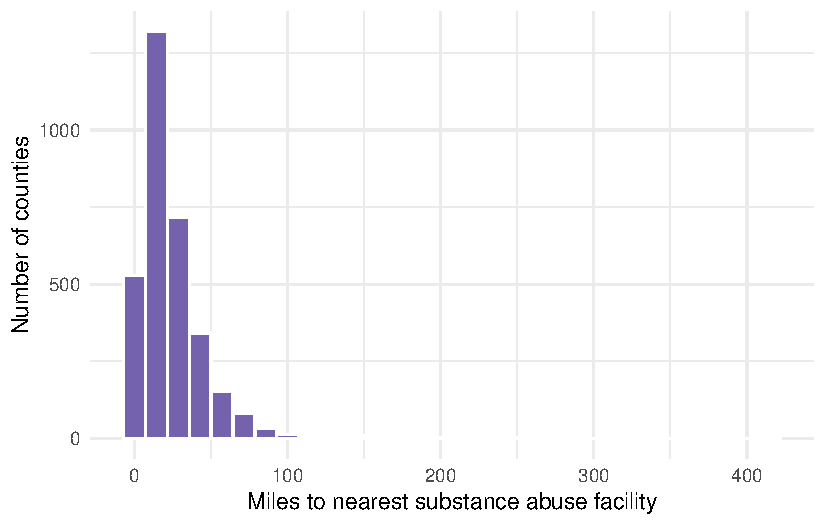
\includegraphics[keepaspectratio]{module4_files/figure-pdf/unnamed-chunk-62-1.pdf}}

\begin{itemize}
\item
  Next, transform the variable to the 4 recommended transformations to
  see which one works best. We cannot see that result yet until we graph
  these results.

  \begin{itemize}
  \tightlist
  \item
    This requires 4 separate calculations using mutate() commands.
  \end{itemize}

\begin{Shaded}
\begin{Highlighting}[]
\NormalTok{dist.mat.cleaned }\OtherTok{\textless{}{-}}\NormalTok{ dist.mat }\SpecialCharTok{\%\textgreater{}\%}
    \FunctionTok{mutate}\NormalTok{(}\AttributeTok{miles.cube.root =}\NormalTok{ VALUE}\SpecialCharTok{\^{}}\NormalTok{(}\DecValTok{1}\SpecialCharTok{/}\DecValTok{3}\NormalTok{)) }\SpecialCharTok{\%\textgreater{}\%}
    \FunctionTok{mutate}\NormalTok{(}\AttributeTok{miles.log =} \FunctionTok{log}\NormalTok{(}\AttributeTok{x =}\NormalTok{ VALUE)) }\SpecialCharTok{\%\textgreater{}\%}
    \FunctionTok{mutate}\NormalTok{(}\AttributeTok{miles.inverse =} \DecValTok{1}\SpecialCharTok{/}\NormalTok{VALUE) }\SpecialCharTok{\%\textgreater{}\%}
    \FunctionTok{mutate}\NormalTok{(}\AttributeTok{miles.sqrt =} \FunctionTok{sqrt}\NormalTok{(}\AttributeTok{x =}\NormalTok{ VALUE))}
\end{Highlighting}
\end{Shaded}
\item
  Now, graph the variable with the 4 recommended transformations to see
  which is most normal (bell shaped).
\end{itemize}

\begin{Shaded}
\begin{Highlighting}[]
\NormalTok{cuberoot }\OtherTok{\textless{}{-}}\NormalTok{ dist.mat.cleaned }\SpecialCharTok{\%\textgreater{}\%}
    \FunctionTok{ggplot}\NormalTok{(}\FunctionTok{aes}\NormalTok{(}\AttributeTok{x =}\NormalTok{ miles.cube.root)) }\SpecialCharTok{+} \FunctionTok{geom\_histogram}\NormalTok{(}\AttributeTok{fill =} \StringTok{"\#7463AC"}\NormalTok{,}
    \AttributeTok{color =} \StringTok{"white"}\NormalTok{) }\SpecialCharTok{+} \FunctionTok{theme\_minimal}\NormalTok{() }\SpecialCharTok{+} \FunctionTok{labs}\NormalTok{(}\AttributeTok{x =} \StringTok{"Cube root of miles to nearest facility"}\NormalTok{,}
    \AttributeTok{y =} \StringTok{"Number of counties"}\NormalTok{)}

\NormalTok{logged }\OtherTok{\textless{}{-}}\NormalTok{ dist.mat.cleaned }\SpecialCharTok{\%\textgreater{}\%}
    \FunctionTok{ggplot}\NormalTok{(}\FunctionTok{aes}\NormalTok{(}\AttributeTok{x =}\NormalTok{ miles.log)) }\SpecialCharTok{+} \FunctionTok{geom\_histogram}\NormalTok{(}\AttributeTok{fill =} \StringTok{"\#7463AC"}\NormalTok{, }\AttributeTok{color =} \StringTok{"white"}\NormalTok{) }\SpecialCharTok{+}
    \FunctionTok{theme\_minimal}\NormalTok{() }\SpecialCharTok{+} \FunctionTok{labs}\NormalTok{(}\AttributeTok{x =} \StringTok{"Log of miles to nearest facility"}\NormalTok{, }\AttributeTok{y =} \StringTok{""}\NormalTok{)}

\NormalTok{inversed }\OtherTok{\textless{}{-}}\NormalTok{ dist.mat.cleaned }\SpecialCharTok{\%\textgreater{}\%}
    \FunctionTok{ggplot}\NormalTok{(}\FunctionTok{aes}\NormalTok{(}\AttributeTok{x =}\NormalTok{ miles.inverse)) }\SpecialCharTok{+} \FunctionTok{geom\_histogram}\NormalTok{(}\AttributeTok{fill =} \StringTok{"\#7463AC"}\NormalTok{, }\AttributeTok{color =} \StringTok{"white"}\NormalTok{) }\SpecialCharTok{+}
    \FunctionTok{theme\_minimal}\NormalTok{() }\SpecialCharTok{+} \FunctionTok{xlim}\NormalTok{(}\DecValTok{0}\NormalTok{, }\DecValTok{1}\NormalTok{) }\SpecialCharTok{+} \FunctionTok{labs}\NormalTok{(}\AttributeTok{x =} \StringTok{"Inverse of miles to nearest facility"}\NormalTok{,}
    \AttributeTok{y =} \StringTok{"Number of counties"}\NormalTok{)}

\NormalTok{squareroot }\OtherTok{\textless{}{-}}\NormalTok{ dist.mat.cleaned }\SpecialCharTok{\%\textgreater{}\%}
    \FunctionTok{ggplot}\NormalTok{(}\FunctionTok{aes}\NormalTok{(}\AttributeTok{x =}\NormalTok{ miles.sqrt)) }\SpecialCharTok{+} \FunctionTok{geom\_histogram}\NormalTok{(}\AttributeTok{fill =} \StringTok{"\#7463AC"}\NormalTok{, }\AttributeTok{color =} \StringTok{"white"}\NormalTok{) }\SpecialCharTok{+}
    \FunctionTok{theme\_minimal}\NormalTok{() }\SpecialCharTok{+} \FunctionTok{labs}\NormalTok{(}\AttributeTok{x =} \StringTok{"Square root of miles to nearest facility"}\NormalTok{,}
    \AttributeTok{y =} \StringTok{""}\NormalTok{)}
\end{Highlighting}
\end{Shaded}

\begin{itemize}
\tightlist
\item
  We can show all 4 graphs at one time to directly compare. Ensure your
  plot window is large enough to see this.
\end{itemize}

\begin{Shaded}
\begin{Highlighting}[]
\NormalTok{gridExtra}\SpecialCharTok{::}\FunctionTok{grid.arrange}\NormalTok{(cuberoot, logged, inversed, squareroot)}
\end{Highlighting}
\end{Shaded}

\pandocbounded{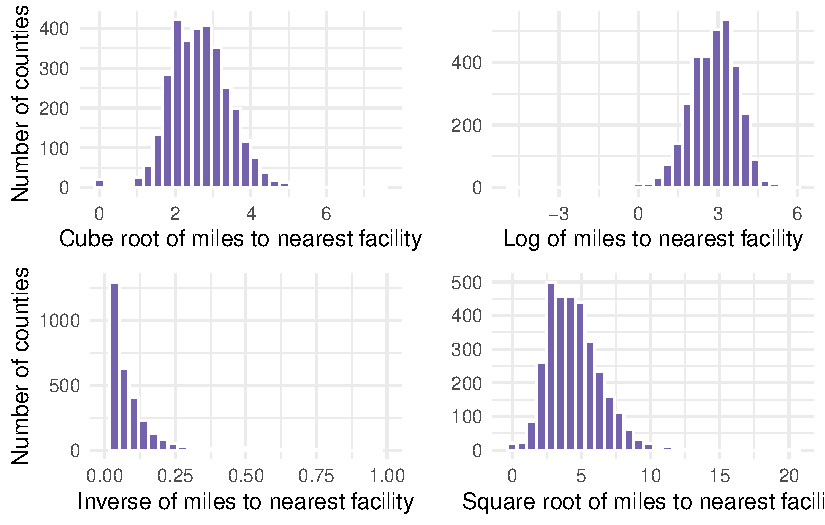
\includegraphics[keepaspectratio]{module4_files/figure-pdf/unnamed-chunk-65-1.pdf}}

\begin{itemize}
\item
  Finally, determine if any of the transformations help. In this
  example, we determined that the cuberoot had the most normal
  transformation. The cube root graph contains a nice bell shape curve.
\item
  Let's use that new variable in the analysis. Start by summarizing the
  descriptive statistics, including retrieving the mean and standard
  deviation for cube root of miles, which are values that are required
  in the probability calculations.
\end{itemize}

\begin{Shaded}
\begin{Highlighting}[]
\NormalTok{dist.mat.cleaned }\SpecialCharTok{\%\textgreater{}\%}
    \FunctionTok{drop\_na}\NormalTok{(miles.cube.root) }\SpecialCharTok{\%\textgreater{}\%}
    \FunctionTok{summarize}\NormalTok{(}\AttributeTok{mean.tran.dist =} \FunctionTok{mean}\NormalTok{(}\AttributeTok{x =}\NormalTok{ miles.cube.root), }\AttributeTok{sd.tran.dist =} \FunctionTok{sd}\NormalTok{(}\AttributeTok{x =}\NormalTok{ miles.cube.root))}
\end{Highlighting}
\end{Shaded}

\begin{verbatim}
  mean.tran.dist sd.tran.dist
1       2.662915    0.7923114
\end{verbatim}

\begin{itemize}
\tightlist
\item
  2.66 and .79 are the values we pulled for mean and standard deviation.
  We can use that information to calculate probabilities based on the
  functions we mentioned above.
\item
  So, what happens if the cuberoot of X \textless{} 3 or less than 27
  miles from the facility?
\item
  We estimate that about 66\% of counties fall in the shaded area,
  having to travel less than 27 miles to nearest facility (27 = 3\^{}3).
\item
  This means that (1- 0.6665403)*100 is the percentage of countries
  having to travel more than 27 miles to the nearest facility.
\end{itemize}

\begin{Shaded}
\begin{Highlighting}[]
\DecValTok{27}\SpecialCharTok{\^{}}\NormalTok{(}\DecValTok{1}\SpecialCharTok{/}\DecValTok{3}\NormalTok{)}
\end{Highlighting}
\end{Shaded}

\begin{verbatim}
[1] 3
\end{verbatim}

\begin{Shaded}
\begin{Highlighting}[]
\DecValTok{3}\SpecialCharTok{\^{}}\DecValTok{3}
\end{Highlighting}
\end{Shaded}

\begin{verbatim}
[1] 27
\end{verbatim}

\begin{Shaded}
\begin{Highlighting}[]
\CommentTok{\# P(X\textless{} cuberoot(27) = P(X \textless{} 3)}
\FunctionTok{pnorm}\NormalTok{(}\DecValTok{3}\NormalTok{, }\FloatTok{2.66}\NormalTok{, }\FloatTok{0.79}\NormalTok{)  }\DocumentationTok{\#\#about 66\% likely}
\end{Highlighting}
\end{Shaded}

\begin{verbatim}
[1] 0.6665403
\end{verbatim}

\begin{Shaded}
\begin{Highlighting}[]
\CommentTok{\# P(X \textgreater{} 3) \#about 33\% likely}
\FunctionTok{pnorm}\NormalTok{(}\DecValTok{3}\NormalTok{, }\FloatTok{2.66}\NormalTok{, }\FloatTok{0.79}\NormalTok{, }\AttributeTok{lower.tail =} \ConstantTok{FALSE}\NormalTok{)}
\end{Highlighting}
\end{Shaded}

\begin{verbatim}
[1] 0.3334597
\end{verbatim}

\begin{Shaded}
\begin{Highlighting}[]
\DecValTok{1} \SpecialCharTok{{-}} \FunctionTok{pnorm}\NormalTok{(}\DecValTok{3}\NormalTok{, }\FloatTok{2.66}\NormalTok{, }\FloatTok{0.79}\NormalTok{)}
\end{Highlighting}
\end{Shaded}

\begin{verbatim}
[1] 0.3334597
\end{verbatim}

\begin{itemize}
\tightlist
\item
  We estimate that about 20\% of counties fall in the shaded area,
  having to travel \textless{} 8 miles to nearest facility (8 = 2\^{}3).
\end{itemize}

\begin{Shaded}
\begin{Highlighting}[]
\FunctionTok{pnorm}\NormalTok{(}\DecValTok{2}\NormalTok{, }\FloatTok{2.66}\NormalTok{, }\FloatTok{0.79}\NormalTok{)}
\end{Highlighting}
\end{Shaded}

\begin{verbatim}
[1] 0.2017342
\end{verbatim}

\begin{itemize}
\tightlist
\item
  We can use the equation to calculate the z-score for a county where
  you have to drive 15 miles to a facility.
\end{itemize}

\begin{Shaded}
\begin{Highlighting}[]
\DocumentationTok{\#\# z = (x{-}m)/sd since we are in cube root {-} we multiply x by \^{}1/3}
\NormalTok{(}\DecValTok{15}\SpecialCharTok{\^{}}\NormalTok{(}\DecValTok{1}\SpecialCharTok{/}\DecValTok{3}\NormalTok{) }\SpecialCharTok{{-}} \FloatTok{2.66}\NormalTok{)}\SpecialCharTok{/}\FloatTok{0.79}
\end{Highlighting}
\end{Shaded}

\begin{verbatim}
[1] -0.2453012
\end{verbatim}

\begin{itemize}
\item
  The transformed distance of a facility 15 miles away is .24 standard
  deviations LOWER than the mean transformed distance.
\item
  Next, we can calculate z for a county with residents who have to
  travel 50 miles to the nearest facility. In the transformed miles
  variable, this would be the cube root of 50, or a value of 3.68.
\end{itemize}

\begin{Shaded}
\begin{Highlighting}[]
\NormalTok{(}\DecValTok{50}\SpecialCharTok{\^{}}\NormalTok{(}\DecValTok{1}\SpecialCharTok{/}\DecValTok{3}\NormalTok{) }\SpecialCharTok{{-}} \FloatTok{2.66}\NormalTok{)}\SpecialCharTok{/}\FloatTok{0.79}  \CommentTok{\#[1] 1.296242}
\end{Highlighting}
\end{Shaded}

\begin{verbatim}
[1] 1.296242
\end{verbatim}

\begin{itemize}
\tightlist
\item
  This indicated that the transformed distance to a facility with MAT
  for this example county was 1.29 standard deviations above the mean
  transformed distance from a county to a facility with MAT.
\end{itemize}

\section{Transformation Second
Example}\label{transformation-second-example}

\begin{itemize}
\tightlist
\item
  Taking a second example, let us look at the PHYSHLTH variable from the
  gender dataset (brfss.csv). We worked with this dataset in an earlier
  lesson. In doing so, we cleaned the data.
\item
  I copied over that data preparation code in regards to the variable of
  interest (PHYSHLTH), and tidied it up for one example. To remind
  ourselves, the question being asked was the following, ``Now thinking
  about your physical health, which includes physical illness and
  injury, for how many days during the past 30 days was your physical
  health not good?''
\item
  If ever you are using the MASS package and dplyr, the select function
  may have a conflict where R does not know which to use. If you get an
  error when using select, add dplyr:: in front of the statement to
  ensure you are using select from dplyr to select variables.
\end{itemize}

\begin{Shaded}
\begin{Highlighting}[]
\CommentTok{\#}
\NormalTok{gender }\OtherTok{\textless{}{-}} \FunctionTok{read.csv}\NormalTok{(}\StringTok{"data/brfss.csv"}\NormalTok{)}
\CommentTok{\# Review the data}
\FunctionTok{summary}\NormalTok{(gender)}
\end{Highlighting}
\end{Shaded}

\begin{verbatim}
    TRNSGNDR        X_AGEG5YR          X_RACE         X_INCOMG    
 Min.   :1.000    Min.   : 1.000   Min.   :1.000   Min.   :1.000  
 1st Qu.:4.000    1st Qu.: 5.000   1st Qu.:1.000   1st Qu.:3.000  
 Median :4.000    Median : 8.000   Median :1.000   Median :5.000  
 Mean   :4.059    Mean   : 7.822   Mean   :1.992   Mean   :4.481  
 3rd Qu.:4.000    3rd Qu.:10.000   3rd Qu.:1.000   3rd Qu.:5.000  
 Max.   :9.000    Max.   :14.000   Max.   :9.000   Max.   :9.000  
 NA's   :310602                    NA's   :94                     
    X_EDUCAG        HLTHPLN1         HADMAM          X_AGE80     
 Min.   :1.000   Min.   :1.000   Min.   :1.000    Min.   :18.00  
 1st Qu.:2.000   1st Qu.:1.000   1st Qu.:1.000    1st Qu.:44.00  
 Median :3.000   Median :1.000   Median :1.000    Median :58.00  
 Mean   :2.966   Mean   :1.108   Mean   :1.215    Mean   :55.49  
 3rd Qu.:4.000   3rd Qu.:1.000   3rd Qu.:1.000    3rd Qu.:69.00  
 Max.   :9.000   Max.   :9.000   Max.   :9.000    Max.   :80.00  
                                 NA's   :208322                  
    PHYSHLTH   
 Min.   : 1.0  
 1st Qu.:20.0  
 Median :88.0  
 Mean   :61.2  
 3rd Qu.:88.0  
 Max.   :99.0  
 NA's   :4     
\end{verbatim}

\begin{Shaded}
\begin{Highlighting}[]
\CommentTok{\# PHYSHLTH example}
\NormalTok{gender.clean }\OtherTok{\textless{}{-}}\NormalTok{ gender }\SpecialCharTok{\%\textgreater{}\%}
\NormalTok{    dplyr}\SpecialCharTok{::}\FunctionTok{select}\NormalTok{(PHYSHLTH) }\SpecialCharTok{\%\textgreater{}\%}
    \FunctionTok{drop\_na}\NormalTok{() }\SpecialCharTok{\%\textgreater{}\%}
    \CommentTok{\# Turn the 77 values to NA, since 77 meant don\textquotesingle{}t know or not sure}
    \CommentTok{\# from the brss codebook}
\FunctionTok{mutate}\NormalTok{(}\AttributeTok{PHYSHLTH =} \FunctionTok{na\_if}\NormalTok{(PHYSHLTH, }\AttributeTok{y =} \DecValTok{77}\NormalTok{)) }\SpecialCharTok{\%\textgreater{}\%}
    \CommentTok{\# Turn the 99 values to NA, since 99 meant Refuled from the brss}
    \CommentTok{\# codebook.}
\FunctionTok{mutate}\NormalTok{(}\AttributeTok{PHYSHLTH =} \FunctionTok{na\_if}\NormalTok{(PHYSHLTH, }\AttributeTok{y =} \DecValTok{99}\NormalTok{)) }\SpecialCharTok{\%\textgreater{}\%}
    \CommentTok{\# Recode the 88 values to 0 {-} since the number 88 meant 0 days of}
    \CommentTok{\# illness from the brss codebook.}
\FunctionTok{mutate}\NormalTok{(}\AttributeTok{PHYSHLTH =} \FunctionTok{recode}\NormalTok{(PHYSHLTH, }\StringTok{\textasciigrave{}}\AttributeTok{88}\StringTok{\textasciigrave{}} \OtherTok{=} \DecValTok{0}\NormalTok{L))}
\FunctionTok{table}\NormalTok{(gender.clean}\SpecialCharTok{$}\NormalTok{PHYSHLTH)}
\end{Highlighting}
\end{Shaded}

\begin{verbatim}

     0      1      2      3      4      5      6      7      8      9     10 
291696  19505  24890  14713   7644  12931   2140   8049   1478    325   9437 
    11     12     13     14     15     16     17     18     19     20     21 
   133    908     92   4558   8638    221    153    279     51   5554   1111 
    22     23     24     25     26     27     28     29     30 
   132     80     98   2270    149    204    831    390  35701 
\end{verbatim}

\begin{Shaded}
\begin{Highlighting}[]
\FunctionTok{summary}\NormalTok{(gender.clean)}
\end{Highlighting}
\end{Shaded}

\begin{verbatim}
    PHYSHLTH     
 Min.   : 0.000  
 1st Qu.: 0.000  
 Median : 0.000  
 Mean   : 4.224  
 3rd Qu.: 3.000  
 Max.   :30.000  
 NA's   :10299   
\end{verbatim}

\begin{itemize}
\tightlist
\item
  Once here, we graph PHYSHLTH.\\
\end{itemize}

\begin{Shaded}
\begin{Highlighting}[]
\NormalTok{gender.clean }\SpecialCharTok{\%\textgreater{}\%}
    \FunctionTok{ggplot}\NormalTok{(}\FunctionTok{aes}\NormalTok{(PHYSHLTH)) }\SpecialCharTok{+} \FunctionTok{geom\_histogram}\NormalTok{(}\AttributeTok{fill =} \StringTok{"\#7463AC"}\NormalTok{, }\AttributeTok{color =} \StringTok{"white"}\NormalTok{) }\SpecialCharTok{+}
    \FunctionTok{theme\_minimal}\NormalTok{() }\SpecialCharTok{+} \FunctionTok{labs}\NormalTok{(}\AttributeTok{x =} \StringTok{"Number of Days Sick"}\NormalTok{, }\AttributeTok{y =} \StringTok{"Frequency"}\NormalTok{)}
\end{Highlighting}
\end{Shaded}

\pandocbounded{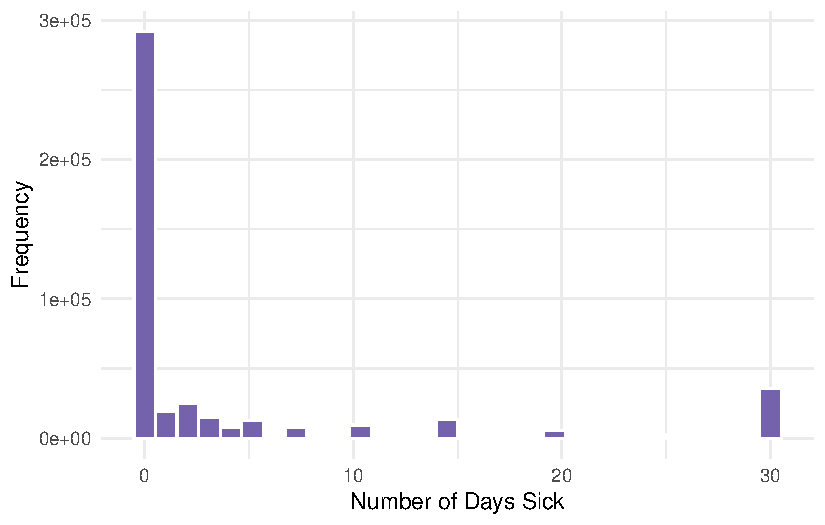
\includegraphics[keepaspectratio]{module4_files/figure-pdf/unnamed-chunk-72-1.pdf}}

\begin{itemize}
\item
  We determined from the descriptive statistics lesson that this
  variable had severe skewness (positive). Most people had 0 days of
  illness.
\item
  Next, we run the 4 calculations by mutating the variable and saving
  all 4 transformation under new variable names.
\end{itemize}

\begin{Shaded}
\begin{Highlighting}[]
\NormalTok{genderTransform }\OtherTok{\textless{}{-}}\NormalTok{ gender.clean }\SpecialCharTok{\%\textgreater{}\%}
    \FunctionTok{mutate}\NormalTok{(}\AttributeTok{phy.cube.root =}\NormalTok{ PHYSHLTH}\SpecialCharTok{\^{}}\NormalTok{(}\DecValTok{1}\SpecialCharTok{/}\DecValTok{3}\NormalTok{)) }\SpecialCharTok{\%\textgreater{}\%}
    \FunctionTok{mutate}\NormalTok{(}\AttributeTok{phy.log =} \FunctionTok{log}\NormalTok{(}\AttributeTok{x =}\NormalTok{ PHYSHLTH)) }\SpecialCharTok{\%\textgreater{}\%}
    \FunctionTok{mutate}\NormalTok{(}\AttributeTok{phy.inverse =} \DecValTok{1}\SpecialCharTok{/}\NormalTok{PHYSHLTH) }\SpecialCharTok{\%\textgreater{}\%}
    \FunctionTok{mutate}\NormalTok{(}\AttributeTok{phy.sqrt =} \FunctionTok{sqrt}\NormalTok{(}\AttributeTok{x =}\NormalTok{ PHYSHLTH))}
\end{Highlighting}
\end{Shaded}

\begin{itemize}
\tightlist
\item
  Next, we create the 4 graphs for each of the 4 transformations
  labelled above to see if one helps.
\end{itemize}

\begin{Shaded}
\begin{Highlighting}[]
\NormalTok{cuberoot }\OtherTok{\textless{}{-}}\NormalTok{ genderTransform }\SpecialCharTok{\%\textgreater{}\%}
    \FunctionTok{ggplot}\NormalTok{(}\FunctionTok{aes}\NormalTok{(}\AttributeTok{x =}\NormalTok{ phy.cube.root)) }\SpecialCharTok{+} \FunctionTok{geom\_histogram}\NormalTok{(}\AttributeTok{fill =} \StringTok{"\#7463AC"}\NormalTok{, }\AttributeTok{color =} \StringTok{"white"}\NormalTok{,}
    \AttributeTok{binwidth =} \FloatTok{0.5}\NormalTok{) }\SpecialCharTok{+} \FunctionTok{theme\_minimal}\NormalTok{() }\SpecialCharTok{+} \FunctionTok{labs}\NormalTok{(}\AttributeTok{x =} \StringTok{"Cube root"}\NormalTok{, }\AttributeTok{y =} \StringTok{""}\NormalTok{)}
\NormalTok{logged }\OtherTok{\textless{}{-}}\NormalTok{ genderTransform }\SpecialCharTok{\%\textgreater{}\%}
    \FunctionTok{ggplot}\NormalTok{(}\FunctionTok{aes}\NormalTok{(}\AttributeTok{x =}\NormalTok{ phy.log)) }\SpecialCharTok{+} \FunctionTok{geom\_histogram}\NormalTok{(}\AttributeTok{fill =} \StringTok{"\#7463AC"}\NormalTok{, }\AttributeTok{color =} \StringTok{"white"}\NormalTok{,}
    \AttributeTok{binwidth =} \FloatTok{0.5}\NormalTok{) }\SpecialCharTok{+} \FunctionTok{theme\_minimal}\NormalTok{() }\SpecialCharTok{+} \FunctionTok{labs}\NormalTok{(}\AttributeTok{x =} \StringTok{"Log"}\NormalTok{, }\AttributeTok{y =} \StringTok{""}\NormalTok{)}
\NormalTok{inversed }\OtherTok{\textless{}{-}}\NormalTok{ genderTransform }\SpecialCharTok{\%\textgreater{}\%}
    \FunctionTok{ggplot}\NormalTok{(}\FunctionTok{aes}\NormalTok{(}\AttributeTok{x =}\NormalTok{ phy.inverse)) }\SpecialCharTok{+} \FunctionTok{xlim}\NormalTok{(}\DecValTok{0}\NormalTok{, }\DecValTok{1}\NormalTok{) }\SpecialCharTok{+} \FunctionTok{geom\_histogram}\NormalTok{(}\AttributeTok{fill =} \StringTok{"\#7463AC"}\NormalTok{,}
    \AttributeTok{color =} \StringTok{"white"}\NormalTok{, }\AttributeTok{binwidth =} \FloatTok{0.05}\NormalTok{) }\SpecialCharTok{+} \FunctionTok{theme\_minimal}\NormalTok{() }\SpecialCharTok{+} \FunctionTok{labs}\NormalTok{(}\AttributeTok{x =} \StringTok{"Inverse"}\NormalTok{,}
    \AttributeTok{y =} \StringTok{""}\NormalTok{)}
\NormalTok{squareroot }\OtherTok{\textless{}{-}}\NormalTok{ genderTransform }\SpecialCharTok{\%\textgreater{}\%}
    \FunctionTok{ggplot}\NormalTok{(}\FunctionTok{aes}\NormalTok{(}\AttributeTok{x =}\NormalTok{ phy.sqrt)) }\SpecialCharTok{+} \FunctionTok{geom\_histogram}\NormalTok{(}\AttributeTok{fill =} \StringTok{"\#7463AC"}\NormalTok{, }\AttributeTok{color =} \StringTok{"white"}\NormalTok{,}
    \AttributeTok{binwidth =} \DecValTok{1}\NormalTok{) }\SpecialCharTok{+} \FunctionTok{theme\_minimal}\NormalTok{() }\SpecialCharTok{+} \FunctionTok{labs}\NormalTok{(}\AttributeTok{x =} \StringTok{"Square root"}\NormalTok{, }\AttributeTok{y =} \StringTok{""}\NormalTok{)}
\end{Highlighting}
\end{Shaded}

\begin{itemize}
\tightlist
\item
  Finally, we plot the graphs using gridExtra so that we can see all 4.
\end{itemize}

\begin{Shaded}
\begin{Highlighting}[]
\NormalTok{gridExtra}\SpecialCharTok{::}\FunctionTok{grid.arrange}\NormalTok{(cuberoot, logged, inversed, squareroot)}
\end{Highlighting}
\end{Shaded}

\pandocbounded{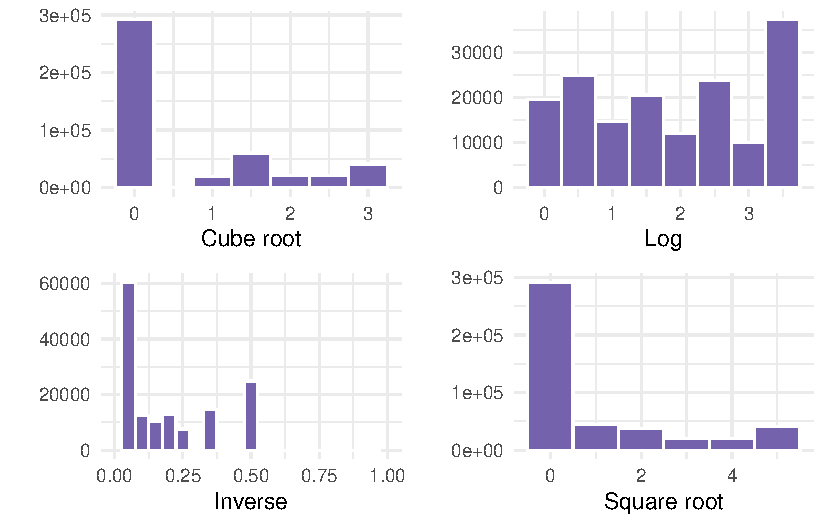
\includegraphics[keepaspectratio]{module4_files/figure-pdf/unnamed-chunk-75-1.pdf}}

\begin{itemize}
\tightlist
\item
  In this example, NOT ONE transformation helped. If this happens,
  something else would need to occur before correctly using the
  variable. Examples could be to run a non-linear model, or categorizing
  the data into bins, especially since there was a large frequency of
  people that were not ill.
\end{itemize}

\bookmarksetup{startatroot}

\chapter{Contingency Tables}\label{contingency-tables}

\begin{itemize}
\tightlist
\item
  A contingency table generally shows frequencies for two qualitative or
  categorical variables, x and y.
\item
  Each cell represents a mutually exclusive combination of the pair of x
  and y values.
\end{itemize}

\begin{figure}[H]

{\centering \pandocbounded{\includegraphics[keepaspectratio]{Pictures/Ch5/ContTableEx.png}}

}

\caption{Contingency Table Example}

\end{figure}%

\begin{itemize}
\tightlist
\item
  Note that each cell in the contingency table represents a frequency.

  \begin{itemize}
  \tightlist
  \item
    In the above table, 174 customers under the age of 35 purchased an
    Under Armour product.
  \item
    54 customers at least 35 years old purchased an Under Armour
    product.
  \end{itemize}
\item
  The contingency table may be used to calculate probabilities using
  relative frequency.

  \begin{itemize}
  \tightlist
  \item
    First obtain the row and column totals.
  \item
    Sample size is equal to the total of the row totals or column
    totals. In this case, n = 600.
  \end{itemize}
\end{itemize}

\section{Probability Rules}\label{probability-rules}

\begin{itemize}
\tightlist
\item
  The addition rule refers to the probability that event A or B occurs,
  or that at least one of these events occurs, is the following:\\
  \[P(A \cup B) = (P(A) + P(B) - P(A \cap B)\]
\item
  The complement rule refers to the probability of the complement of an
  event, \(P(A^c)\) is equal to one minus the probability of the
  event.\\
  \[P(A^c) = 1-P(A)\]
\item
  Conditional probability refers to the probability of an event given
  that another event has already occurred.

  \begin{itemize}
  \tightlist
  \item
    Given two events A and B, each with a positive probability of
    occurring, the probability that A occurs given that B has occurred
    (A conditioned on B) is equals to \(P(A|B) = (P(A \cap B)/P(B)\).
    Similarly, the probability that B occurs given that A has occurred
    (B conditioned on A) is equal to \(P(B|A) = (P(B \cap A)/P(A)\).
  \end{itemize}
\item
  Marginal probability refers to the probability of an event occurring
  \((P(A))\), it may be thought of as an unconditional probability. It
  is not conditioned on another event.
\item
  The joint probability rule is determined by dividing each cell
  frequency by the grand total. Joint probability refers to the
  statistical measure that calculates the likelihood of two events
  occurring together and at the same point in time.\\
  \[P(A \cap B)\]

  \begin{itemize}
  \tightlist
  \item
    For example, the probability that a randomly selected person is
    under 35 years of age and makes an Under Armour purchase is
    \(P(U35 \cap UA)=174/600= .29\)
  \end{itemize}
\item
  For example, this Venn Diagram illustrates the sample space for events
  A and B.
\item
  The union of two events (\(A \cup B\)) is the event consisting of all
  simple events in A or B.
\end{itemize}

\pandocbounded{\includegraphics[keepaspectratio]{Pictures/Ch5/Venn1.png}}
The intersection of two events (\(A \cap B\)) consists of all simple
events in both A and B.

\begin{figure}[H]

{\centering \pandocbounded{\includegraphics[keepaspectratio]{Pictures/Ch5/Venn2.png}}

}

\caption{Venn Diagram: Intersection and Union}

\end{figure}%

\begin{itemize}
\tightlist
\item
  The complement of event A (i.e., \(A^c\)) is the event consisting of
  all simple events in the sample space S that are not in A.
\end{itemize}

\begin{figure}[H]

{\centering \pandocbounded{\includegraphics[keepaspectratio]{Pictures/Ch5/Venn3.png}}

}

\caption{Venn Diagram: Complement Rule}

\end{figure}%

\section{Summary Measures for a Random
Variable}\label{summary-measures-for-a-random-variable-1}

\begin{itemize}
\tightlist
\item
  The Summary Measures of a Random Variable are consistent with our
  discussion of Probability in the last lesson. They are copied back
  here for ease of reference.
\end{itemize}

\subsection{Expected Value}\label{expected-value-1}

\begin{itemize}
\tightlist
\item
  We can calculate the expected value, or value we think is going to
  occur based on the type of distribution.

  \begin{itemize}
  \tightlist
  \item
    Expected value is also known as the population mean \(\mu\), and is
    the weighted average of all possible values of \(X\).
  \item
    More specifically, \(E(X)\) is the long-run average value of the
    random variable over infinitely many independent repetitions of an
    experiment.
  \item
    For a discrete random variable \(X\) with values
    \(x_1, x_2, x_3, ...\) that occur with probabilities \(P(X=x_i)\),
    the expected value of \(X\) is the probability weighted average of
    the values. In the case of one random variable, that means:
    \[E(X) = \mu = \sum{x_iP(X=x_i)} = n*p\]
  \end{itemize}
\end{itemize}

\subsection{Variance}\label{variance-1}

\begin{itemize}
\tightlist
\item
  Variance of a random variable is the average of the squared
  differences from the mean.

  \begin{itemize}
  \tightlist
  \item
    For a discrete random variable \(X\) with values
    \(x_1, x_2, x_3, ...\) that occur with probabilities \(P(X=x_i)\),
    the variance is defined as:
    \[Var(X) = \sigma^2 = \sum{(x_i-\mu)^2*P(X=x_i)} = n*p*(1-p)\]
  \end{itemize}
\end{itemize}

\subsection{Standard Deviation}\label{standard-deviation-1}

\begin{itemize}
\tightlist
\item
  Standard deviation is consistently the square root of the variance.
  \[SD(X) = \sigma = \sqrt{\sigma^2} = \sqrt{\sum{(x_i-\mu)^2*P(X=x_i)}}= \sqrt{np*(1-p)}\]
\end{itemize}

\section{Calculating Probability}\label{calculating-probability}

\begin{itemize}
\tightlist
\item
  We could calculate the statistics in this contingency table a couple
  of ways. First, we could manually calculate it like below.
\end{itemize}

\begin{Shaded}
\begin{Highlighting}[]
\DocumentationTok{\#\# Calculate Totals}
\NormalTok{TotalUnder35 }\OtherTok{\textless{}{-}} \DecValTok{174} \SpecialCharTok{+} \DecValTok{132} \SpecialCharTok{+} \DecValTok{90}
\NormalTok{TotalUnder35  }\DocumentationTok{\#\#Total under 35 age group}
\end{Highlighting}
\end{Shaded}

\begin{verbatim}
[1] 396
\end{verbatim}

\begin{Shaded}
\begin{Highlighting}[]
\NormalTok{Total35up }\OtherTok{\textless{}{-}} \DecValTok{54} \SpecialCharTok{+} \DecValTok{72} \SpecialCharTok{+} \DecValTok{78}
\NormalTok{Total35up  }\DocumentationTok{\#\# Total 35 and older}
\end{Highlighting}
\end{Shaded}

\begin{verbatim}
[1] 204
\end{verbatim}

\begin{Shaded}
\begin{Highlighting}[]
\NormalTok{TotalUA }\OtherTok{\textless{}{-}} \DecValTok{174} \SpecialCharTok{+} \DecValTok{54}
\NormalTok{TotalUA  }\DocumentationTok{\#\# Total Under Armour}
\end{Highlighting}
\end{Shaded}

\begin{verbatim}
[1] 228
\end{verbatim}

\begin{Shaded}
\begin{Highlighting}[]
\NormalTok{TotalNike }\OtherTok{\textless{}{-}} \DecValTok{132} \SpecialCharTok{+} \DecValTok{72}
\NormalTok{TotalNike  }\DocumentationTok{\#\# Total Nike}
\end{Highlighting}
\end{Shaded}

\begin{verbatim}
[1] 204
\end{verbatim}

\begin{Shaded}
\begin{Highlighting}[]
\NormalTok{TotalAdidas }\OtherTok{\textless{}{-}} \DecValTok{90} \SpecialCharTok{+} \DecValTok{78}
\NormalTok{TotalAdidas  }\DocumentationTok{\#\# Total Adidas}
\end{Highlighting}
\end{Shaded}

\begin{verbatim}
[1] 168
\end{verbatim}

\begin{Shaded}
\begin{Highlighting}[]
\NormalTok{Total }\OtherTok{\textless{}{-}} \DecValTok{174} \SpecialCharTok{+} \DecValTok{132} \SpecialCharTok{+} \DecValTok{90} \SpecialCharTok{+} \DecValTok{54} \SpecialCharTok{+} \DecValTok{72} \SpecialCharTok{+} \DecValTok{78}
\NormalTok{Total  }\DocumentationTok{\#\#Grand Total }
\end{Highlighting}
\end{Shaded}

\begin{verbatim}
[1] 600
\end{verbatim}

\begin{itemize}
\tightlist
\item
  Alternatively, we could make this a matrix and use the matrix command
  to help us calculate the answer. This gives us all the statistics with
  a couple of functions and allows us to interpret from there after
  selecting the right information from the output.
\end{itemize}

\begin{Shaded}
\begin{Highlighting}[]
\CommentTok{\# Put observed values in a vector by row.}
\NormalTok{x }\OtherTok{\textless{}{-}} \FunctionTok{c}\NormalTok{(}\DecValTok{174}\NormalTok{, }\DecValTok{132}\NormalTok{, }\DecValTok{90}\NormalTok{, }\DecValTok{54}\NormalTok{, }\DecValTok{72}\NormalTok{, }\DecValTok{78}\NormalTok{)}
\CommentTok{\# Turn the vector into a matrix. In this case, we had 2 rows, 3}
\CommentTok{\# columns, and entered the data by row.}
\NormalTok{o }\OtherTok{\textless{}{-}} \FunctionTok{matrix}\NormalTok{(x, }\DecValTok{2}\NormalTok{, }\DecValTok{3}\NormalTok{, }\AttributeTok{byrow =} \ConstantTok{TRUE}\NormalTok{)}
\NormalTok{o}
\end{Highlighting}
\end{Shaded}

\begin{verbatim}
     [,1] [,2] [,3]
[1,]  174  132   90
[2,]   54   72   78
\end{verbatim}

\begin{Shaded}
\begin{Highlighting}[]
\CommentTok{\# Next, we could add the names of the columns and rows values using}
\CommentTok{\# the dimnames() command.}
\FunctionTok{dimnames}\NormalTok{(o) }\OtherTok{\textless{}{-}} \FunctionTok{list}\NormalTok{(}\FunctionTok{c}\NormalTok{(}\StringTok{"Under 35"}\NormalTok{, }\StringTok{"35 and Older"}\NormalTok{), }\FunctionTok{c}\NormalTok{(}\StringTok{"Under Armour"}\NormalTok{, }\StringTok{"Nike"}\NormalTok{,}
    \StringTok{"Adidas"}\NormalTok{))}
\NormalTok{o}
\end{Highlighting}
\end{Shaded}

\begin{verbatim}
             Under Armour Nike Adidas
Under 35              174  132     90
35 and Older           54   72     78
\end{verbatim}

\begin{Shaded}
\begin{Highlighting}[]
\CommentTok{\# We can easily calculate the total from here.}
\NormalTok{total }\OtherTok{\textless{}{-}} \FunctionTok{sum}\NormalTok{(o)}
\NormalTok{total}
\end{Highlighting}
\end{Shaded}

\begin{verbatim}
[1] 600
\end{verbatim}

\begin{Shaded}
\begin{Highlighting}[]
\NormalTok{rowsums }\OtherTok{\textless{}{-}} \FunctionTok{margin.table}\NormalTok{(o, }\DecValTok{1}\NormalTok{)}
\NormalTok{rowsums}
\end{Highlighting}
\end{Shaded}

\begin{verbatim}
    Under 35 35 and Older 
         396          204 
\end{verbatim}

\begin{Shaded}
\begin{Highlighting}[]
\NormalTok{colsums }\OtherTok{\textless{}{-}} \FunctionTok{margin.table}\NormalTok{(o, }\DecValTok{2}\NormalTok{)}
\NormalTok{colsums}
\end{Highlighting}
\end{Shaded}

\begin{verbatim}
Under Armour         Nike       Adidas 
         228          204          168 
\end{verbatim}

\begin{Shaded}
\begin{Highlighting}[]
\NormalTok{prob }\OtherTok{\textless{}{-}} \FunctionTok{prop.table}\NormalTok{(o)}
\NormalTok{prob  }\CommentTok{\# each cell represents a joint probability}
\end{Highlighting}
\end{Shaded}

\begin{verbatim}
             Under Armour Nike Adidas
Under 35             0.29 0.22   0.15
35 and Older         0.09 0.12   0.13
\end{verbatim}

\begin{Shaded}
\begin{Highlighting}[]
\NormalTok{rowprob }\OtherTok{\textless{}{-}} \FunctionTok{margin.table}\NormalTok{(prob, }\DecValTok{1}\NormalTok{)}
\NormalTok{rowprob  }\CommentTok{\#each value represents marginal probability}
\end{Highlighting}
\end{Shaded}

\begin{verbatim}
    Under 35 35 and Older 
        0.66         0.34 
\end{verbatim}

\begin{Shaded}
\begin{Highlighting}[]
\NormalTok{colprob }\OtherTok{\textless{}{-}} \FunctionTok{margin.table}\NormalTok{(prob, }\DecValTok{2}\NormalTok{)}
\NormalTok{colprob  }\CommentTok{\#each value represents marginal probability}
\end{Highlighting}
\end{Shaded}

\begin{verbatim}
Under Armour         Nike       Adidas 
        0.38         0.34         0.28 
\end{verbatim}

\begin{itemize}
\tightlist
\item
  Take note that when subsetting from the matrix we created above, the
  dimnames do not serve as a column or row. so the first number is in
  row 1, column 1. This is distinct from data.frames, which typically
  have the 1st column designated for the labels.
\end{itemize}

\begin{Shaded}
\begin{Highlighting}[]
\NormalTok{prob[}\DecValTok{1}\NormalTok{, }\DecValTok{1}\NormalTok{]  }\CommentTok{\#corresponds to the joint probability value associated with Row 1 (Under 35), Col 1 (Under Armour)}
\end{Highlighting}
\end{Shaded}

\begin{verbatim}
[1] 0.29
\end{verbatim}

\begin{itemize}
\item
  Once we do our calculations our totals, we can ask probability
  questions.
\item
  When looking up an answer to the question, it makes it easier to
  reference the tables to ensure you are subsetting correctly.
\end{itemize}

\begin{Shaded}
\begin{Highlighting}[]
\NormalTok{o}
\end{Highlighting}
\end{Shaded}

\begin{verbatim}
             Under Armour Nike Adidas
Under 35              174  132     90
35 and Older           54   72     78
\end{verbatim}

\begin{Shaded}
\begin{Highlighting}[]
\NormalTok{prob}
\end{Highlighting}
\end{Shaded}

\begin{verbatim}
             Under Armour Nike Adidas
Under 35             0.29 0.22   0.15
35 and Older         0.09 0.12   0.13
\end{verbatim}

\begin{itemize}
\tightlist
\item
  If a person is under 35, what is the probability they will select
  Under Armour? \[P(UA|under35) = (P(UA \cap under35)/P(under35))\]
\end{itemize}

\begin{Shaded}
\begin{Highlighting}[]
\CommentTok{\# This is a conditional probability question.}
\DecValTok{174}\SpecialCharTok{/}\DecValTok{396}  \CommentTok{\#or}
\end{Highlighting}
\end{Shaded}

\begin{verbatim}
[1] 0.4393939
\end{verbatim}

\begin{Shaded}
\begin{Highlighting}[]
\FloatTok{0.29}\SpecialCharTok{/}\FloatTok{0.66}  \CommentTok{\#or}
\end{Highlighting}
\end{Shaded}

\begin{verbatim}
[1] 0.4393939
\end{verbatim}

\begin{Shaded}
\begin{Highlighting}[]
\NormalTok{prob[}\DecValTok{1}\NormalTok{, }\DecValTok{1}\NormalTok{]}\SpecialCharTok{/}\NormalTok{rowprob[}\DecValTok{1}\NormalTok{]}
\end{Highlighting}
\end{Shaded}

\begin{verbatim}
 Under 35 
0.4393939 
\end{verbatim}

\begin{itemize}
\tightlist
\item
  What is the probability of a person 35 or older randomly selecting
  Nike? \[P(N|older35) = (P(N \cap older35)/P(older35))\]
\end{itemize}

\begin{Shaded}
\begin{Highlighting}[]
\CommentTok{\# This is a conditional probability question.}
\DecValTok{72}\SpecialCharTok{/}\DecValTok{204}  \CommentTok{\# or}
\end{Highlighting}
\end{Shaded}

\begin{verbatim}
[1] 0.3529412
\end{verbatim}

\begin{Shaded}
\begin{Highlighting}[]
\FloatTok{0.12}\SpecialCharTok{/}\FloatTok{0.34}  \CommentTok{\# or}
\end{Highlighting}
\end{Shaded}

\begin{verbatim}
[1] 0.3529412
\end{verbatim}

\begin{Shaded}
\begin{Highlighting}[]
\NormalTok{prob[}\DecValTok{2}\NormalTok{, }\DecValTok{2}\NormalTok{]}\SpecialCharTok{/}\NormalTok{rowprob[}\DecValTok{2}\NormalTok{]}
\end{Highlighting}
\end{Shaded}

\begin{verbatim}
35 and Older 
   0.3529412 
\end{verbatim}

\begin{itemize}
\tightlist
\item
  If the chance the preference was the same regardless of condition, how
  many people would you expect to select Nike? \[Ex(Nike)\]
\end{itemize}

\begin{Shaded}
\begin{Highlighting}[]
\CommentTok{\# This is a expected value question.}
\NormalTok{TotalNike  }\CommentTok{\# or}
\end{Highlighting}
\end{Shaded}

\begin{verbatim}
[1] 204
\end{verbatim}

\begin{Shaded}
\begin{Highlighting}[]
\NormalTok{colsums[}\DecValTok{2}\NormalTok{]}
\end{Highlighting}
\end{Shaded}

\begin{verbatim}
Nike 
 204 
\end{verbatim}

\begin{itemize}
\tightlist
\item
  We can calculate summary measures based on a variable category.
\end{itemize}

\begin{Shaded}
\begin{Highlighting}[]
\CommentTok{\# E(X) of 35 Years or older (formula n*p)}
\NormalTok{n }\OtherTok{\textless{}{-}}\NormalTok{ total}
\NormalTok{n  }\CommentTok{\#600}
\end{Highlighting}
\end{Shaded}

\begin{verbatim}
[1] 600
\end{verbatim}

\begin{Shaded}
\begin{Highlighting}[]
\NormalTok{p }\OtherTok{\textless{}{-}}\NormalTok{ rowprob[}\DecValTok{2}\NormalTok{]}
\NormalTok{p  }\CommentTok{\#.34}
\end{Highlighting}
\end{Shaded}

\begin{verbatim}
35 and Older 
        0.34 
\end{verbatim}

\begin{Shaded}
\begin{Highlighting}[]
\NormalTok{n }\SpecialCharTok{*}\NormalTok{ p  }\CommentTok{\#Or simply the frequency for the column 35 and older}
\end{Highlighting}
\end{Shaded}

\begin{verbatim}
35 and Older 
         204 
\end{verbatim}

\begin{Shaded}
\begin{Highlighting}[]
\CommentTok{\# Var(X) (formula n*p*(1{-}p))}
\NormalTok{varx }\OtherTok{\textless{}{-}}\NormalTok{ n }\SpecialCharTok{*}\NormalTok{ p }\SpecialCharTok{*}\NormalTok{ (}\DecValTok{1} \SpecialCharTok{{-}}\NormalTok{ p)}
\NormalTok{varx  }\CommentTok{\#134.64}
\end{Highlighting}
\end{Shaded}

\begin{verbatim}
35 and Older 
      134.64 
\end{verbatim}

\begin{Shaded}
\begin{Highlighting}[]
\CommentTok{\# SD(X) (formula sqrt of variance)}
\NormalTok{sdx }\OtherTok{\textless{}{-}} \FunctionTok{sqrt}\NormalTok{(varx)}
\NormalTok{sdx  }\CommentTok{\#11.60345 }
\end{Highlighting}
\end{Shaded}

\begin{verbatim}
35 and Older 
    11.60345 
\end{verbatim}

\section{Larger Contingency Table}\label{larger-contingency-table}

\begin{itemize}
\tightlist
\item
  The survey question asked participants in multiple groups the
  following question, ``How likely are you to participate in the event
  in the future?''
\item
  In order to answer this question, first, lets bring in some data and
  calculate totals.
\end{itemize}

\begin{figure}[H]

{\centering \pandocbounded{\includegraphics[keepaspectratio]{Pictures/Ch5/ConTblNum.png}}

}

\caption{Contingency Table Numbers}

\end{figure}%

\begin{Shaded}
\begin{Highlighting}[]
\NormalTok{x }\OtherTok{\textless{}{-}} \FunctionTok{c}\NormalTok{(}\DecValTok{197}\NormalTok{, }\DecValTok{388}\NormalTok{, }\DecValTok{230}\NormalTok{, }\DecValTok{103}\NormalTok{, }\DecValTok{137}\NormalTok{, }\DecValTok{98}\NormalTok{, }\DecValTok{20}\NormalTok{, }\DecValTok{18}\NormalTok{, }\DecValTok{18}\NormalTok{, }\DecValTok{13}\NormalTok{, }\DecValTok{58}\NormalTok{, }\DecValTok{45}\NormalTok{)}
\NormalTok{o }\OtherTok{\textless{}{-}} \FunctionTok{matrix}\NormalTok{(x, }\DecValTok{4}\NormalTok{, }\DecValTok{3}\NormalTok{, }\AttributeTok{byrow =} \ConstantTok{TRUE}\NormalTok{)}
\NormalTok{o}
\end{Highlighting}
\end{Shaded}

\begin{verbatim}
     [,1] [,2] [,3]
[1,]  197  388  230
[2,]  103  137   98
[3,]   20   18   18
[4,]   13   58   45
\end{verbatim}

\begin{Shaded}
\begin{Highlighting}[]
\FunctionTok{dimnames}\NormalTok{(o) }\OtherTok{\textless{}{-}} \FunctionTok{list}\NormalTok{(}\FunctionTok{c}\NormalTok{(}\StringTok{"Students"}\NormalTok{, }\StringTok{"Faculty/Staff"}\NormalTok{, }\StringTok{"Alumni"}\NormalTok{, }\StringTok{"Town Residents"}\NormalTok{),}
    \FunctionTok{c}\NormalTok{(}\StringTok{"Unlikely"}\NormalTok{, }\StringTok{"Moderately Likely"}\NormalTok{, }\StringTok{"Very Likely"}\NormalTok{))}
\NormalTok{o}
\end{Highlighting}
\end{Shaded}

\begin{verbatim}
               Unlikely Moderately Likely Very Likely
Students            197               388         230
Faculty/Staff       103               137          98
Alumni               20                18          18
Town Residents       13                58          45
\end{verbatim}

\begin{Shaded}
\begin{Highlighting}[]
\NormalTok{total }\OtherTok{\textless{}{-}} \FunctionTok{sum}\NormalTok{(o)}
\NormalTok{total}
\end{Highlighting}
\end{Shaded}

\begin{verbatim}
[1] 1325
\end{verbatim}

\begin{Shaded}
\begin{Highlighting}[]
\NormalTok{rowsums }\OtherTok{\textless{}{-}} \FunctionTok{margin.table}\NormalTok{(o, }\DecValTok{1}\NormalTok{)}
\NormalTok{rowsums}
\end{Highlighting}
\end{Shaded}

\begin{verbatim}
      Students  Faculty/Staff         Alumni Town Residents 
           815            338             56            116 
\end{verbatim}

\begin{Shaded}
\begin{Highlighting}[]
\NormalTok{colsums }\OtherTok{\textless{}{-}} \FunctionTok{margin.table}\NormalTok{(o, }\DecValTok{2}\NormalTok{)}
\NormalTok{colsums}
\end{Highlighting}
\end{Shaded}

\begin{verbatim}
         Unlikely Moderately Likely       Very Likely 
              333               601               391 
\end{verbatim}

\begin{Shaded}
\begin{Highlighting}[]
\CommentTok{\# Lets add the grand total to the colsums}
\NormalTok{colsums }\OtherTok{\textless{}{-}} \FunctionTok{c}\NormalTok{(colsums, total)}
\NormalTok{colsums}
\end{Highlighting}
\end{Shaded}

\begin{verbatim}
         Unlikely Moderately Likely       Very Likely                   
              333               601               391              1325 
\end{verbatim}

\begin{itemize}
\tightlist
\item
  In this example, we can bind the data together so that it is a little
  easier to see. Examine the final table and compare that to the figure
  above.
\end{itemize}

\begin{Shaded}
\begin{Highlighting}[]
\NormalTok{totals }\OtherTok{\textless{}{-}} \FunctionTok{cbind}\NormalTok{(o, rowsums)}
\NormalTok{totals}
\end{Highlighting}
\end{Shaded}

\begin{verbatim}
               Unlikely Moderately Likely Very Likely rowsums
Students            197               388         230     815
Faculty/Staff       103               137          98     338
Alumni               20                18          18      56
Town Residents       13                58          45     116
\end{verbatim}

\begin{Shaded}
\begin{Highlighting}[]
\NormalTok{totals }\OtherTok{\textless{}{-}} \FunctionTok{rbind}\NormalTok{(totals, colsums)}
\NormalTok{totals}
\end{Highlighting}
\end{Shaded}

\begin{verbatim}
               Unlikely Moderately Likely Very Likely rowsums
Students            197               388         230     815
Faculty/Staff       103               137          98     338
Alumni               20                18          18      56
Town Residents       13                58          45     116
colsums             333               601         391    1325
\end{verbatim}

\begin{figure}[H]

{\centering \pandocbounded{\includegraphics[keepaspectratio]{Pictures/Ch5/ConTblProp.png}}

}

\caption{Contingency Table Proportions}

\end{figure}%

\begin{itemize}
\tightlist
\item
  Next, let's calculate probabilities.
\end{itemize}

\begin{Shaded}
\begin{Highlighting}[]
\NormalTok{prob }\OtherTok{\textless{}{-}} \FunctionTok{prop.table}\NormalTok{(o)}
\NormalTok{prob}
\end{Highlighting}
\end{Shaded}

\begin{verbatim}
                  Unlikely Moderately Likely Very Likely
Students       0.148679245        0.29283019  0.17358491
Faculty/Staff  0.077735849        0.10339623  0.07396226
Alumni         0.015094340        0.01358491  0.01358491
Town Residents 0.009811321        0.04377358  0.03396226
\end{verbatim}

\begin{Shaded}
\begin{Highlighting}[]
\NormalTok{TotalRowProb }\OtherTok{\textless{}{-}} \FunctionTok{margin.table}\NormalTok{(prob, }\DecValTok{1}\NormalTok{)}
\NormalTok{TotalRowProb}
\end{Highlighting}
\end{Shaded}

\begin{verbatim}
      Students  Faculty/Staff         Alumni Town Residents 
    0.61509434     0.25509434     0.04226415     0.08754717 
\end{verbatim}

\begin{Shaded}
\begin{Highlighting}[]
\NormalTok{TotalColProb }\OtherTok{\textless{}{-}} \FunctionTok{margin.table}\NormalTok{(prob, }\DecValTok{2}\NormalTok{)}
\NormalTok{TotalColProb}
\end{Highlighting}
\end{Shaded}

\begin{verbatim}
         Unlikely Moderately Likely       Very Likely 
        0.2513208         0.4535849         0.2950943 
\end{verbatim}

\begin{Shaded}
\begin{Highlighting}[]
\NormalTok{TotalColProb }\OtherTok{\textless{}{-}} \FunctionTok{c}\NormalTok{(TotalColProb, }\FunctionTok{sum}\NormalTok{(TotalColProb))}
\NormalTok{TotalColProb}
\end{Highlighting}
\end{Shaded}

\begin{verbatim}
         Unlikely Moderately Likely       Very Likely                   
        0.2513208         0.4535849         0.2950943         1.0000000 
\end{verbatim}

\begin{itemize}
\tightlist
\item
  In this example, we can also bind the data together so that it is a
  little easier to see. Again, we are trying to get our R code in the
  best shape to be able to select the right information to calculate
  probability from it.
\end{itemize}

\begin{Shaded}
\begin{Highlighting}[]
\NormalTok{proportions }\OtherTok{\textless{}{-}} \FunctionTok{cbind}\NormalTok{(prob, TotalRowProb)}
\NormalTok{proportions}
\end{Highlighting}
\end{Shaded}

\begin{verbatim}
                  Unlikely Moderately Likely Very Likely TotalRowProb
Students       0.148679245        0.29283019  0.17358491   0.61509434
Faculty/Staff  0.077735849        0.10339623  0.07396226   0.25509434
Alumni         0.015094340        0.01358491  0.01358491   0.04226415
Town Residents 0.009811321        0.04377358  0.03396226   0.08754717
\end{verbatim}

\begin{Shaded}
\begin{Highlighting}[]
\NormalTok{proportions }\OtherTok{\textless{}{-}} \FunctionTok{rbind}\NormalTok{(proportions, TotalColProb)}
\NormalTok{proportions}
\end{Highlighting}
\end{Shaded}

\begin{verbatim}
                  Unlikely Moderately Likely Very Likely TotalRowProb
Students       0.148679245        0.29283019  0.17358491   0.61509434
Faculty/Staff  0.077735849        0.10339623  0.07396226   0.25509434
Alumni         0.015094340        0.01358491  0.01358491   0.04226415
Town Residents 0.009811321        0.04377358  0.03396226   0.08754717
TotalColProb   0.251320755        0.45358491  0.29509434   1.00000000
\end{verbatim}

\begin{itemize}
\item
  Now that our tables have been tabulated, we can answer some
  probability questions.
\item
  What proportion of Students participated in the survey?\\
  \(P_S= 815/1325\) or \(0.61509434\)
\item
  What proportion of Faculty/Staff remarked that they were Unlikely to
  participate?\\
  \(P(U|FS) = P(U \cap FS) / P(FS) = 103/338 = 0.077735849/0.25509434 = 0.3047337\)
\item
  If a person is a Town Resident, what is the probability that they will
  select Very Likely?\\
  \(P(VL|TR) = P(VL \cap TR) / P(TR) = 45/116 = 0.03396226/0.08754717 = 0.387931\)
\item
  What proportion of people would you expect to select Moderately
  Likely?\\
  \(P_ML = 601/1325\) or \(0.4535849\).
\item
  What is the expected number of people would you expect to select
  Moderately Likely? \(E(ML) = 601\).
\item
  What is the probability that a randomly selected person is a
  Faculty/Staff or selects Very Likely?\\
  \(P_FS + P_VL - P_FS \cup P_VL = 0.25509434 + 0.2950943 − 0.07396226 = 0.4762264\)
\end{itemize}

\begin{Shaded}
\begin{Highlighting}[]
\CommentTok{\# E(X) of Moderately Likely (formula n*p)}
\NormalTok{n }\OtherTok{=}\NormalTok{ total}
\NormalTok{n  }\CommentTok{\#1325}
\end{Highlighting}
\end{Shaded}

\begin{verbatim}
[1] 1325
\end{verbatim}

\begin{Shaded}
\begin{Highlighting}[]
\NormalTok{p }\OtherTok{=}\NormalTok{ TotalColProb[}\DecValTok{2}\NormalTok{]}
\NormalTok{p  }\CommentTok{\#.45358}
\end{Highlighting}
\end{Shaded}

\begin{verbatim}
Moderately Likely 
        0.4535849 
\end{verbatim}

\begin{Shaded}
\begin{Highlighting}[]
\NormalTok{n }\SpecialCharTok{*}\NormalTok{ p  }\CommentTok{\#Or simply the frequency for the column Moderately Likely}
\end{Highlighting}
\end{Shaded}

\begin{verbatim}
Moderately Likely 
              601 
\end{verbatim}

\begin{Shaded}
\begin{Highlighting}[]
\CommentTok{\# Var(X) (formula n*p*(1{-}p))}
\NormalTok{varx }\OtherTok{\textless{}{-}}\NormalTok{ n }\SpecialCharTok{*}\NormalTok{ p }\SpecialCharTok{*}\NormalTok{ (}\DecValTok{1} \SpecialCharTok{{-}}\NormalTok{ p)}
\NormalTok{varx  }\CommentTok{\#328.3955}
\end{Highlighting}
\end{Shaded}

\begin{verbatim}
Moderately Likely 
         328.3955 
\end{verbatim}

\begin{Shaded}
\begin{Highlighting}[]
\CommentTok{\# SD(X) (formula sqrt of variance)}
\NormalTok{sdx }\OtherTok{\textless{}{-}} \FunctionTok{sqrt}\NormalTok{(varx)}
\NormalTok{sdx  }\CommentTok{\#18.12}
\end{Highlighting}
\end{Shaded}

\begin{verbatim}
Moderately Likely 
         18.12169 
\end{verbatim}

\bookmarksetup{startatroot}

\chapter{Chi-Squared Test for
Independence}\label{chi-squared-test-for-independence}

\begin{itemize}
\item
  Broadly, the test for independence tests whether or not two variables
  whose frequencies are represented in a contingency table have
  statistical independence from one another.
\item
  A test of independence -- also called a chi-square test of a
  contingency table -- is used to analyze the relationship between two
  qualitative variables.
\item
  Broadly, this test involves summing the squared differences between
  observed and expected values, combining the differences into an
  overall statistic, and then using that statistic to determine
  significance of the hypothesis test.\\
  \(\chi^2 = \frac{(observed-expected)^2}{expected}\)
\item
  Squaring the differences before adding them up will result in a
  positive value that is larger when there are larger differences and
  smaller when there are smaller differences. This value captures the
  magnitude of the difference between observed and expected values.
\item
  In order to account for situations when the observed and expected
  values are very large, which could result in extremely large
  differences between observed and expected, the squared differences are
  divided by the expected value in each cell.
\item
  Visualizing the Chi-squared Distribution Chi-squared distribution has
  a single parameter, the degrees of freedom or \(df\).\\
  The standard deviation of the chi-squared distribution is
  \(\sqrt{2 \cdot df}\). The degrees of freedom in a chi-squared test of
  independence are calculated as the Number of rows−1 multiplied by
  Number ofcolumns−1 or more formally: \(df=(𝑟−1)∗(𝑐−1)\) The larger the
  contingency table, the more degrees of freedom, the wider the
  distribution and more normal it becomes.
\end{itemize}

\pandocbounded{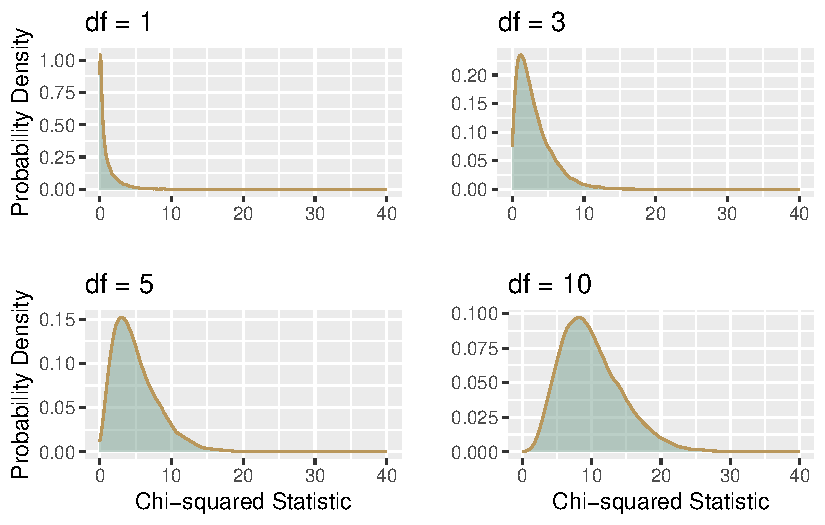
\includegraphics[keepaspectratio]{module4_files/figure-pdf/unnamed-chunk-89-1.pdf}}

\begin{itemize}
\tightlist
\item
  The Chi-Squared Distribution is noted by:

  \begin{itemize}
  \tightlist
  \item
    Right-Skewed:For low degrees of freedom, the chi-squared
    distribution is highly right-skewed. As the degrees of freedom
    increase, the skewness decreases.
  \item
    Non-Negative Values: The chi-squared distribution is defined only
    for non-negative values because it is the sum of squared values.
  \item
    Mean and Variance: The mean of a chi-squared distribution with k
    degrees of freedom is k. The variance is 2k.
  \end{itemize}
\item
  The Chi-squared probability density function shows the probability of
  a value of chi-squared occurring when there is no relationship between
  the two variables contributing to the chi-squared, where a large
  chi-square indicates a relationship between variables.
\item
  The competing hypotheses can be expressed as:

  \begin{itemize}
  \tightlist
  \item
    \(H_0\): The two classifications are independent.
  \item
    \(H_A\): The two classifications are dependent.
  \end{itemize}
\end{itemize}

\pandocbounded{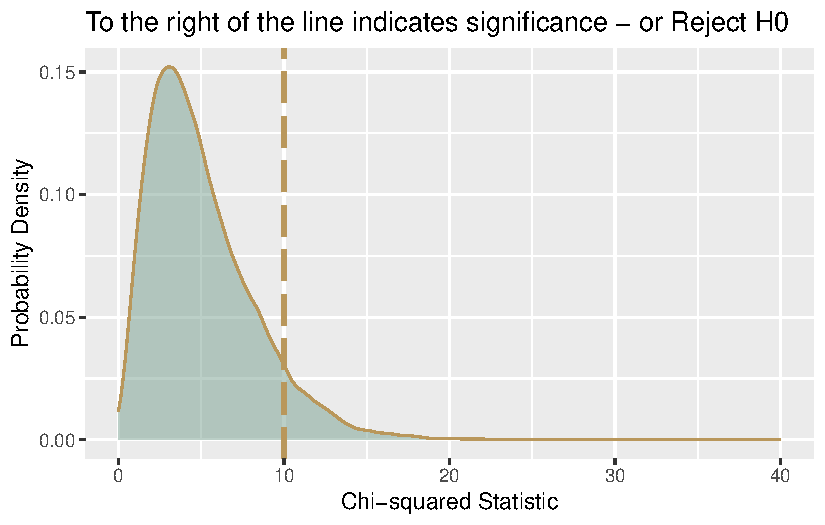
\includegraphics[keepaspectratio]{module4_files/figure-pdf/unnamed-chunk-90-1.pdf}}

\section{Steps to conduct Chi-Squared Test for
Independence}\label{steps-to-conduct-chi-squared-test-for-independence}

\begin{itemize}
\tightlist
\item
  Step 1: Write the null and alternate hypotheses.
\item
  Step 2: Compute the test statistic and calculate the probability.
\item
  Step 3: State a conclusion. If the probability that the null is true
  is very small, usually less than 5\%, reject the null hypothesis OR If
  the probability that the null is true is not small, usually 5\% or
  greater, retain the null hypothesis.
\end{itemize}

\section{Assumptions of the Chi-Squared Test of
Independence}\label{assumptions-of-the-chi-squared-test-of-independence}

\begin{itemize}
\item
  Assumption 1: The variables must be nominal or ordinal.
\item
  Assumption 2: The expected values should be 5 or higher in at least
  80\% of groups.
\item
  Assumption 3: The observations must be independent.
\item
  Note that there are a couple of ways observations can be
  non-independent.

  \begin{itemize}
  \tightlist
  \item
    One way to violate this assumption would be if the data included the
    same set of people before and after some intervention or treatment.
  \item
    Another way to violate this assumption would be for the data to
    include siblings or parents and children or spouses or other people
    who are somehow linked to one another.
  \item
    Since people who are linked to each other often have similar
    characteristics, statistical tests need to be able to account for
    this and the chi-squared test does not.
  \end{itemize}
\end{itemize}

\section{Example of a Test for
Independence}\label{example-of-a-test-for-independence}

\begin{figure}[H]

{\centering \pandocbounded{\includegraphics[keepaspectratio]{Pictures/Ch5/ContTableEx.png}}

}

\caption{Contingency Table Example}

\end{figure}%

\begin{itemize}
\tightlist
\item
  Step 1: Set up the Hypothesis

  \begin{itemize}
  \tightlist
  \item
    \(H_0\): Age group and Brand Name are independent.
  \item
    \(H_A\): Age group and Brand Name are dependent.
  \end{itemize}
\item
  First, we bring in the data manually from the table by column. We had
  3 columns, so we need to make three vectors as shown below.
\end{itemize}

\begin{Shaded}
\begin{Highlighting}[]
\NormalTok{UA }\OtherTok{\textless{}{-}} \FunctionTok{c}\NormalTok{(}\DecValTok{174}\NormalTok{, }\DecValTok{54}\NormalTok{)}
\NormalTok{N }\OtherTok{\textless{}{-}} \FunctionTok{c}\NormalTok{(}\DecValTok{132}\NormalTok{, }\DecValTok{72}\NormalTok{)}
\NormalTok{A }\OtherTok{\textless{}{-}} \FunctionTok{c}\NormalTok{(}\DecValTok{90}\NormalTok{, }\DecValTok{78}\NormalTok{)}
\end{Highlighting}
\end{Shaded}

\begin{itemize}
\tightlist
\item
  Then we convert these variables into a data frame. If you already have
  a data frame, you don't have to do this step.
\end{itemize}

\begin{Shaded}
\begin{Highlighting}[]
\NormalTok{M }\OtherTok{\textless{}{-}} \FunctionTok{data.frame}\NormalTok{(UA, N, A)}
\NormalTok{M}
\end{Highlighting}
\end{Shaded}

\begin{verbatim}
   UA   N  A
1 174 132 90
2  54  72 78
\end{verbatim}

\begin{itemize}
\item
  Always make sure your data frame looks like the table.
\item
  Step 2: Compute the test statistic and calculate the probability.
\item
  Here, we run the chisq.test() command, which only includes the columns
  of interest.
\end{itemize}

\begin{Shaded}
\begin{Highlighting}[]
\FunctionTok{chisq.test}\NormalTok{(M)}
\end{Highlighting}
\end{Shaded}

\begin{verbatim}

    Pearson's Chi-squared test

data:  M
X-squared = 22.529, df = 2, p-value = 1.282e-05
\end{verbatim}

\begin{itemize}
\tightlist
\item
  Step 3: If the probability that the null is true is very small,
  usually less than 5\%, reject the null hypothesis versus If the
  probability that the null is true is not small, usually 5\% or
  greater, retain the null hypothesis.
\item
  Here, our p-value is 1.282e-05, so we reject the null, \(H_0\), and
  conclude that Age group and Brand Names are dependent.
\end{itemize}

\(df=(𝑟−1)∗(𝑐−1)\) or \((2−1)∗(3−1)=1∗2= 2df\)

\subsection{Using a matrix instead of a
data.frame}\label{using-a-matrix-instead-of-a-data.frame}

\begin{itemize}
\tightlist
\item
  You can use either a matrix or a data.frame when solving a chi-squared
  problem.
\item
  In a Chi-squared test of independence, a matrix can be used to
  organize observed frequencies into categories along two dimensions. In
  the example, the matrix o contains data for different age groups
  (``Under 35'' and ``35 and older'') and their brand preferences
  (``Under Armour,'' ``Nike,'' and ``Adidas''). By setting up the matrix
  with these dimensions, the test evaluates whether there is a
  significant association between age group and brand preference. The
  test compares the observed counts with expected counts under the
  assumption that the two variables are independent.
\end{itemize}

\begin{Shaded}
\begin{Highlighting}[]
\NormalTok{x }\OtherTok{\textless{}{-}} \FunctionTok{c}\NormalTok{(}\DecValTok{174}\NormalTok{, }\DecValTok{132}\NormalTok{, }\DecValTok{90}\NormalTok{, }\DecValTok{54}\NormalTok{, }\DecValTok{72}\NormalTok{, }\DecValTok{78}\NormalTok{)}
\NormalTok{o }\OtherTok{\textless{}{-}} \FunctionTok{matrix}\NormalTok{(x, }\AttributeTok{nrow =} \DecValTok{2}\NormalTok{, }\AttributeTok{ncol =} \DecValTok{3}\NormalTok{, }\AttributeTok{byrow =} \ConstantTok{TRUE}\NormalTok{)}
\DocumentationTok{\#\# add some dimnames to o}
\FunctionTok{dimnames}\NormalTok{(o) }\OtherTok{\textless{}{-}} \FunctionTok{list}\NormalTok{(}\FunctionTok{c}\NormalTok{(}\StringTok{"Under 35"}\NormalTok{, }\StringTok{"35 and older"}\NormalTok{), }\FunctionTok{c}\NormalTok{(}\StringTok{"Under Armour"}\NormalTok{, }\StringTok{"Nike"}\NormalTok{,}
    \StringTok{"Adidas"}\NormalTok{))}
\NormalTok{o}
\end{Highlighting}
\end{Shaded}

\begin{verbatim}
             Under Armour Nike Adidas
Under 35              174  132     90
35 and older           54   72     78
\end{verbatim}

\begin{Shaded}
\begin{Highlighting}[]
\FunctionTok{chisq.test}\NormalTok{(o)}
\end{Highlighting}
\end{Shaded}

\begin{verbatim}

    Pearson's Chi-squared test

data:  o
X-squared = 22.529, df = 2, p-value = 1.282e-05
\end{verbatim}

\begin{Shaded}
\begin{Highlighting}[]
\CommentTok{\# \textbackslash{}tPearson\textquotesingle{}s Chi{-}squared test data: o X{-}squared = 22.529, df = 2,}
\CommentTok{\# p{-}value = 0.00001282}
\end{Highlighting}
\end{Shaded}

\begin{itemize}
\tightlist
\item
  In either case, we should see the same result. The result includes the
  Chi-squared statistic (X-squared = 22.529), degrees of freedom (df =
  2), and a very small p-value (0.00001282), indicating a strong
  association between age and brand preference.
\end{itemize}

\section{Example Using an Imported
Dataset}\label{example-using-an-imported-dataset}

\begin{itemize}
\tightlist
\item
  Import the STEM data into a data frame (table) into R.
\item
  Step 1: Set up the Hypothesis:

  \begin{itemize}
  \tightlist
  \item
    \(H_0\): Stem field and Gender are independent.
  \item
    \(H_A\): Stem field and Gender are dependent.
  \end{itemize}
\end{itemize}

\begin{Shaded}
\begin{Highlighting}[]
\NormalTok{STEM }\OtherTok{\textless{}{-}} \FunctionTok{read.csv}\NormalTok{(}\StringTok{"data/stem.csv"}\NormalTok{)}
\NormalTok{STEM}
\end{Highlighting}
\end{Shaded}

\begin{verbatim}
   STEM.field Female Male
1    Sciences    120  100
2  Technology     15   75
3 Engineering     30  125
4        Math     15   20
\end{verbatim}

\begin{itemize}
\tightlist
\item
  Step 2: Compute the test statistic and calculate the probability.
\item
  Again, we use Rs chisq.test() command to calculate the value of the
  test statistic, as well as the p-value. Within the chisq.test()
  function, we indicate that the relevant data are in columns 2 and 3 of
  the data frame.
\end{itemize}

\begin{Shaded}
\begin{Highlighting}[]
\FunctionTok{chisq.test}\NormalTok{(STEM[, }\DecValTok{2}\SpecialCharTok{:}\DecValTok{3}\NormalTok{])}
\end{Highlighting}
\end{Shaded}

\begin{verbatim}

    Pearson's Chi-squared test

data:  STEM[, 2:3]
X-squared = 66.795, df = 3, p-value = 2.072e-14
\end{verbatim}

\begin{Shaded}
\begin{Highlighting}[]
\DocumentationTok{\#\# test statistic: 66.795 df: 3 {-}{-}{-} 4 rows and 2 columns}
\NormalTok{(}\DecValTok{4} \SpecialCharTok{{-}} \DecValTok{1}\NormalTok{) }\SpecialCharTok{*}\NormalTok{ (}\DecValTok{2} \SpecialCharTok{{-}} \DecValTok{1}\NormalTok{)  }\CommentTok{\#3 df}
\end{Highlighting}
\end{Shaded}

\begin{verbatim}
[1] 3
\end{verbatim}

\begin{Shaded}
\begin{Highlighting}[]
\DocumentationTok{\#\# p{-}value is almost 0}
\end{Highlighting}
\end{Shaded}

\begin{itemize}
\item
  Step 3: If the probability that the null is true is very small,
  usually less than 5\%, reject the null hypothesis versus If the
  probability that the null is true is not small, usually 5\% or
  greater, retain the null hypothesis.
\item
  Since the p-value is less than 0.05, we can reject the null
  hypothesis. At the 5\% significance level, we can conclude that one's
  sex does influence field choice within the STEM major.
\item
  When performing a Chi-squared test, the choice of including or
  excluding columns depends on which categories you want to analyze. In
  chisq.test(stem{[}, -1{]}), the first column is excluded, and the test
  is run on the remaining columns. This might be done if the first
  column represents data not relevant to the specific hypothesis you are
  testing (e.g., it could be an identifier or a control category).
\item
  On the other hand, chisq.test(stem{[}, 2:3{]}) only includes the
  second and third columns, focusing the analysis on specific categories
  of interest.
\item
  This is useful when you want to investigate the relationship between
  two particular variables, ignoring other columns that might be
  extraneous to the question you're asking. Including or excluding
  columns is guided by the research hypothesis and the variables you
  want to test for independence.
\end{itemize}

\begin{Shaded}
\begin{Highlighting}[]
\FunctionTok{chisq.test}\NormalTok{(STEM[, }\SpecialCharTok{{-}}\DecValTok{1}\NormalTok{])  }\DocumentationTok{\#\#\# when we subset we use object[row, columns] {-}{-}{-} so including the numbers 2:3 means we include variables in the 2nd and 3rd columns. Including the number {-}1 after the comma means that we exclude the first column. }
\end{Highlighting}
\end{Shaded}

\begin{verbatim}

    Pearson's Chi-squared test

data:  STEM[, -1]
X-squared = 66.795, df = 3, p-value = 2.072e-14
\end{verbatim}

\bookmarksetup{startatroot}

\chapter{Chi-Squared Goodness of Fit
Test}\label{chi-squared-goodness-of-fit-test}

\begin{itemize}
\item
  There are a few other tests regarding a Chi-squared distribution, and
  one other is the goodness of fit test.
\item
  This test determines whether two or more population proportions equal
  each other or any predetermined set of values and like the test for
  independence, still involves the fit between observed and estimated
  values.
\item
  A multinomial experiment consists of a series of n independent trials
  such that:
\item
  On each there are k possible outcomes.
\item
  The probability of falling into category \(i\) is the same on each
  trial.
\item
  The \(k\) probabilities sum to \(1:p_1 + p_2 +⋯+p_k = 1\)
\item
  The null hypothesis: the population proportions are equal to one
  another or they are each equal to a specific value.
\item
  For example, are four candidates in an election equally favored by
  voters?
\item
  Equal Population proportions:\\
  \(H_0: P_1=P_2=P_3=P_4=.25;\)\\
  \(H_A\):Not all populations are equal to .25
\item
  Or, do people rate food quality in a restaurant comparably to last
  year?
\item
  Unequal Population Proportions:\\
  \(H_0: P_1= .4, P_2=.3, P_3= .2, P_4=.1;\)\\
  \(H_A:\) At least one \(P_i\) differs from its hypothesized value.
\end{itemize}

\section{Example Using Raw Numbers}\label{example-using-raw-numbers}

\begin{itemize}
\item
  Last year the management at a restaurant surveyed its patrons to rate
  the quality of its food. The results were as follows: 15\% Excellent;
  30\% Good; 45\% Fair; and 10\% Poor.
\item
  Based on this and other survey results, management made changes to the
  menu.
\item
  This year, the management surveyed 250 patrons, asking the same
  questions about food quality. Here are the results: 46 Excellent; 83
  Good; 105 Fair; and 16 Poor.
\item
  We want to know if the current results agree with those from last
  year, or if there has been a significant change.
\item
  To do this, we compute an expected frequency for each category and
  compare it to what we actually observe. Then, we compute the
  difference between what was observed and expected for each category.
  If the results this year are consistent with last year, these
  differences will be relatively small.
\item
  The steps are same as the Chi-Squared Test of Independence.
\item
  Step 1: Set up the Hypothesis:

  \begin{itemize}
  \tightlist
  \item
    \(𝐻_0\): Each proportion equals a hypothesized value.
  \item
    \(𝐻_A\): Not all proportions equal their hypothesized values.
  \end{itemize}
\item
  Step 2: Compute the test statistic and calculate the probability.
\item
  We can use R's chisq.test() function to calculate the value of the
  test statistic and corresponding p-value. Within this function, we use
  the option p to indicate the location of the hypothesized
  proportions.\\
\end{itemize}

\begin{Shaded}
\begin{Highlighting}[]
\CommentTok{\# Chi Squared Test Goodness of Fit}
\NormalTok{o }\OtherTok{\textless{}{-}} \FunctionTok{c}\NormalTok{(}\DecValTok{46}\NormalTok{, }\DecValTok{83}\NormalTok{, }\DecValTok{105}\NormalTok{, }\DecValTok{16}\NormalTok{)}
\NormalTok{p }\OtherTok{\textless{}{-}} \FunctionTok{c}\NormalTok{(}\FloatTok{0.15}\NormalTok{, }\FloatTok{0.3}\NormalTok{, }\FloatTok{0.45}\NormalTok{, }\FloatTok{0.1}\NormalTok{)}

\DocumentationTok{\#\# quick check on p}
\FunctionTok{sum}\NormalTok{(p)  }\DocumentationTok{\#\#1: sum of all proportions should be 1}
\end{Highlighting}
\end{Shaded}

\begin{verbatim}
[1] 1
\end{verbatim}

\begin{Shaded}
\begin{Highlighting}[]
\CommentTok{\# run the test}
\FunctionTok{chisq.test}\NormalTok{(o, }\AttributeTok{p =}\NormalTok{ p)}
\end{Highlighting}
\end{Shaded}

\begin{verbatim}

    Chi-squared test for given probabilities

data:  o
X-squared = 6.52, df = 3, p-value = 0.08888
\end{verbatim}

\begin{Shaded}
\begin{Highlighting}[]
\CommentTok{\# test statistic: 6.52 df: 3 {-}{-}{-}{-}{-} 4 proportions {-} 1 {-}{-} or}
\DecValTok{4} \SpecialCharTok{{-}} \DecValTok{1}  \DocumentationTok{\#\#3}
\end{Highlighting}
\end{Shaded}

\begin{verbatim}
[1] 3
\end{verbatim}

\begin{Shaded}
\begin{Highlighting}[]
\CommentTok{\# p{-}value is 0.08888 \textgreater{} .05}
\end{Highlighting}
\end{Shaded}

\begin{itemize}
\item
  Note that p= is required here because it is not the second argument in
  the chisq.test() command.
\item
  Step 3: If the probability that the null is true is very small,
  usually less than 5\%, reject the null hypothesis versus If the
  probability that the null is true is not small, usually 5\% or
  greater, retain the null hypothesis.
\item
  At alpha = .05, we do not reject \(H_0\) and cannot conclude that the
  proportions differ from the ones a year ago.
\end{itemize}

\section{Example Using an Imported
Dataset}\label{example-using-an-imported-dataset-1}

\begin{itemize}
\tightlist
\item
  The steps are same as the Chi-Squared Test of Independence.
\item
  Step 1: Set up the Hypothesis:

  \begin{itemize}
  \tightlist
  \item
    \(𝐻_0\): Each proportion equals a hypothesized value.
  \item
    \(𝐻_A\): Not all proportions equal their hypothesized values.
  \end{itemize}
\item
  Step 2: Compute the test statistic and calculate the probability.
\item
  First, we import the stemGOF.csv data into a data frame (table) in R.
\item
  Then, again, we use Rs chisq.test function to calculate the value of
  the test statistic and the p-value. Within the chisq.test function, we
  use the option p to indicate the location of the hypothesized
  proportions.
\end{itemize}

\begin{Shaded}
\begin{Highlighting}[]
\NormalTok{STEMGOF }\OtherTok{\textless{}{-}} \FunctionTok{read.csv}\NormalTok{(}\StringTok{"data/stemGOF.csv"}\NormalTok{)}
\NormalTok{STEMGOF}
\end{Highlighting}
\end{Shaded}

\begin{verbatim}
            Major X2010Proportions RecentNumbers
1        Business             0.19            80
2       Education             0.09            35
3      Healthcare             0.12            85
4 Social Sciences             0.22           105
5            STEM             0.08            55
6           Other             0.30           140
\end{verbatim}

\begin{Shaded}
\begin{Highlighting}[]
\FunctionTok{chisq.test}\NormalTok{(STEMGOF}\SpecialCharTok{$}\NormalTok{RecentNumbers, }\AttributeTok{p =}\NormalTok{ STEMGOF}\SpecialCharTok{$}\NormalTok{X2010Proportions)}
\end{Highlighting}
\end{Shaded}

\begin{verbatim}

    Chi-squared test for given probabilities

data:  STEMGOF$RecentNumbers
X-squared = 21.526, df = 5, p-value = 0.0006441
\end{verbatim}

\begin{Shaded}
\begin{Highlighting}[]
\CommentTok{\# Chi{-}squared test for given probabilities data:}
\CommentTok{\# stemGOF$RecentNumbers X{-}squared = 21.526, df = 5, p{-}value =}
\CommentTok{\# 0.0006441 df: 6 options so 6{-}1 is 5 test statistic is back high:}
\CommentTok{\# 21. 526}
\end{Highlighting}
\end{Shaded}

\begin{itemize}
\tightlist
\item
  Step 3: If the probability that the null is true is very small,
  usually less than 5\%, reject the null hypothesis versus If the
  probability that the null is true is not small, usually 5\% or
  greater, retain the null hypothesis.
\item
  Since our p-value is 0.0006441, we reject \(H_0\) and conclude that
  the proportions differ at the 5\% significance level. In this case,
  that means that the recent stem numbers differ from the 2010 values.
\end{itemize}

\bookmarksetup{startatroot}

\chapter{Using AI}\label{using-ai-3}

\begin{itemize}
\item
  Use the following prompts on a generative AI, like chatGPT, to learn
  more about probability and contingency tables.
\item
  What is a contingency table, and how is it used to represent the
  relationship between two categorical variables in probability
  calculations?
\item
  How do you calculate joint, marginal, and conditional probabilities
  using a contingency table, and what is the significance of each type
  of probability?
\item
  Can you explain how the chi-squared test for independence works, and
  how it is used to determine whether two categorical variables are
  independent or dependent?
\item
  What is the difference between the chi-squared test for independence
  and the chi-squared goodness of fit test, and how is each test
  applied?
\item
  Once you calculate the chi-squared test statistic, how do you
  interpret the p-value to determine whether to reject or fail to reject
  the null hypothesis?
\item
  Why are degrees of freedom important in a chi-squared test, and how do
  you calculate them for a contingency table?
\item
  How do you set up and execute a chi-squared test using the
  chisq.test() function in R, and what are the key outputs to focus on
  when interpreting the results?
\item
  What are the key characteristics of a probability distribution, and
  how do you determine whether a given set of values represents a valid
  probability distribution?
\item
  What is the difference between a discrete and a continuous random
  variable, and how do the probability distributions differ for each
  type?
\item
  How do you calculate the expected value and variance for a discrete
  random variable, and why are these summary measures important in
  understanding probability distributions?
\item
  What are the properties of a binomial distribution, and how is it used
  to calculate the probability of a certain number of successes in a
  fixed number of trials?
\item
  How do you use the dbinom() and pbinom() functions in R to calculate
  the probability of exact or cumulative successes in a binomial
  experiment?
\item
  What is a normal distribution, and how do you calculate z-scores to
  determine how far an observation is from the mean of a normally
  distributed variable?
\item
  How do you interpret and calculate cumulative probabilities for both
  discrete and continuous variables using the cumulative distribution
  function (CDF)''
\item
  What is the Central Limit Theorem (CLT), and why is it important when
  working with large samples and understanding the distribution of
  sample means?
\item
  When data is not normally distributed, what transformations can you
  apply to make the data more normally distributed, and how do you
  determine which transformation is most effective?
\item
  How do you apply probability functions such as pnorm() and qnorm() in
  R to solve real-world problems, such as calculating the likelihood of
  events based on normal distributions?
\end{itemize}

\bookmarksetup{startatroot}

\chapter{Summary}\label{summary-4}

\begin{itemize}
\item
  In this lesson, we learned about the basic rules of probability
  alongside the binomial distribution and continuous distribution. We
  learned about the normal distribution and the limitations of using
  that distribution. We also learned how to transform variables that
  were not normal.
\item
  In a normal distribution, we used 3 main formulas with the pnorm()
  function. Each formula has a different role, but they all provide a
  way to assess variability relative to an average value, allowing for
  comparisons and inferences about the data or sample in question.
\end{itemize}

\begin{array}{|c|c|c|c|}
\hline
\textbf{Context} & \textbf{Formula} & \textbf{Interpretation} & \textbf{pnorm Function Usage} \\
\hline
\text{Standardizing individual data points} & \frac{x - \text{mean}(x)}{\text{sd}(x)} & \text{Z-score for individual values} & \text{pnorm}(x, \text{mean}, \text{sd}) \\
\hline
\text{Standardizing the sample mean} & \frac{x - \text{mean}(x)}{\text{sd}(x) / \sqrt{n}} & \text{Used for hypothesis tests of means} & \text{pnorm}(x, \text{mean}, \text{se}) \\
\hline
\text{Standardizing a sample proportion} & \frac{\hat{p} - p}{\sqrt{\frac{p(1 - p)}{n}}} & \text{Used for hypothesis tests of proportions} & \text{pnorm}(\hat{p}, p, \sqrt{\frac{p(1 - p)}{n}}) \\
\hline
\end{array}

\begin{itemize}
\tightlist
\item
  We also learned about contingency tables in regards to calculating
  probability with two categorical variables. We also computed the
  chi-squared statistics for the test of independence and the goodness
  of fit.
\item
  We note that the ``Goodness of fit'' and ``test of independence'' are
  both chi-square tests, but they serve different purposes:
\item
  Goodness of Fit test: \emph{Purpose}: Assesses how well observed data
  match a specified distribution (often a theoretical or expected
  distribution). \emph{Example}: Checking if the distribution of colors
  of M\&M's in a bag matches the expected company distribution (say,
  30\% blue, 20\% red, etc.). \emph{Null Hypothesis}: The observed
  frequencies match the expected frequencies.
\item
  Test of Independence: \emph{Purpose}: Determines whether there is a
  significant association between two categorical variables in a
  contingency table. \emph{Example}: Evaluating if gender (male/female)
  is independent of preference for a type of product (e.g., A or B).
  \emph{Null Hypothesis}: The two variables are independent (no
  association).
\end{itemize}

\bookmarksetup{startatroot}

\chapter{Module 5: Hypothesis
Testing}\label{module-5-hypothesis-testing}

\begin{itemize}
\tightlist
\item
  The goal of this lesson is to teach you how to conduct statistical
  inference with regards to hypothesis testing. In doing so, we will
  learn a few key hypothesis tests given t-distributions, including the
  one-sample t-test, the independent samples t-test, and the dependent
  samples t-test. We will continue to conduct hypothesis tests in the
  later modules as they are the cornerstone to conducting sound
  statistical inference.
\end{itemize}

\subsection{At a Glance}\label{at-a-glance-4}

\begin{itemize}
\tightlist
\item
  In order to succeed in this section, you will need to understand how
  to set up and test a hypothesis, knowing that we can reuse our logic
  of hypothesis testing for other types of models later on. Pay close
  attention to the idea of and the reason for the t-distribution with
  regards to one-sample, independent samples, and dependent samples
  hypothesis test. Additionally, note when the test is a two-tailed, a
  right-tailed, or a left-tailed test, and what that means for the
  interpretation of the results.
\end{itemize}

\subsection{Lesson Objectives}\label{lesson-objectives-4}

\begin{itemize}
\tightlist
\item
  Compare a sample mean to a population mean with a one-sample t-test.
\item
  Compare two unrelated sample means with an independent-samples t-test.
\item
  Compare two related sample means with a dependent-samples t-test.
\item
  Compare and contrast the the three t-tests covered in this module:
  one-sample, independent samples, and dependent samples.
\end{itemize}

\subsection{Consider While Reading}\label{consider-while-reading-4}

\begin{itemize}
\tightlist
\item
  In this lesson, we learn more about hypothesis testing, which will
  continue throughout the rest of the term! We are still conducting
  inference analysis. As an analyst, I like to say that this starts the
  fun stuff.
\item
  We cover three important t-tests. There are more examples on the our
  course management system with regards to setting up a two-tailed,
  right-tailed, or left-tailed test and adjusting the \(\mu\) of
  interest.
\item
  Make sure you understand the key differences between all the three
  t-tests presented in this module and their role in interpreting data
  and making inferences. All three tests are making comparisons:
  comparisons to a mean value, comparison to another population, or
  comparison to paired data like before and after results.
\end{itemize}

\section{Hypothesis Testing}\label{hypothesis-testing}

\begin{itemize}
\tightlist
\item
  A hypothesis test resolves conflicts between two competing opinions
  (hypotheses).
\item
  In a hypothesis test, we define the null hypothesis as \(H_0\), which
  is the presumed default state of nature or status quo. We define the
  alternative hypothesis as \(H_A\), \emph{a contradiction of the}
  default state of nature or status quo.
\item
  In statistics we use sample information to make inferences regarding
  the unknown population parameters of interest. We conduct hypothesis
  tests to determine if sample evidence contradicts \(H_0\).

  \begin{itemize}
  \tightlist
  \item
    On the basis of sample information, we either ``Reject the null
    hypothesis'' in which sample evidence is inconsistent with \(H_0\).
    This means that we show support for our alternative hypothesis,
    \(H_A\).
  \item
    Or we ``Do not reject the null hypothesis.'' in which the sample
    evidence is not inconsistent with \(H_0\); or we do not have enough
    evidence to ``accept'' \(H_0\). This means that there is no support
    for our alternative hypothesis, \(H_A\).
  \end{itemize}
\item
  General guidelines:

  \begin{itemize}
  \tightlist
  \item
    Null hypothesis, \(H_0\), states the status quo.
  \item
    Alternative hypothesis, \(H_A\), states whatever we wish to
    establish (i.e., contests the status quo).
  \end{itemize}
\item
  Use the following signs in hypothesis tests:

  \begin{itemize}
  \tightlist
  \item
    \(H_0\): \(=\) or \(>=\) or \(<=\) to specify status quo.
  \item
    \(H_A\): \(\neq\) or \(<\) or \(>\) to contradict \(H_0\).
  \end{itemize}
\item
  Where \(H_0\) always contains the equality sign.
\end{itemize}

\subsection{Hypothesis Testing Covers a Variety of
Tests}\label{hypothesis-testing-covers-a-variety-of-tests}

\begin{itemize}
\tightlist
\item
  We will cover the following:
\end{itemize}

\begin{enumerate}
\def\labelenumi{\arabic{enumi}.}
\tightlist
\item
  One-Sample t-test;
\item
  Independent samples t-test;
\item
  Dependent (or Paired) samples t-test.
\end{enumerate}

\subsection{Using a t-Distribution}\label{using-a-t-distribution}

\begin{itemize}
\tightlist
\item
  All of these hypothesis tests listed above use a t-distribution, which
  is like a z-distribution (i.e., z-score), but specifically accounts
  for some specific population information being unknown.

  \begin{itemize}
  \tightlist
  \item
    The z-distribution shows how many sample standard deviations (SD)
    some value is away from the mean.
  \item
    The t-distribution shows how many standard errors (SE) some value is
    away from the mean.
  \end{itemize}
\item
  All of these hypothesis tests in the assigned readings use the
  t.test() command to execute in R with different parameters set.
\end{itemize}

\subsection{Approaches to Hypothesis
Testing}\label{approaches-to-hypothesis-testing}

\begin{itemize}
\item
  All approaches to scientific hypothesis testing enable us to determine
  whether the sample evidence is inconsistent with what is hypothesized
  under the null hypothesis, \(H_0\).
\item
  Basic principle: First assume that \(H_0\) is true and then determine
  if sample evidence contradicts this assumption.
\item
  This means that we can never assume our claim (against status quo) is
  supported without rejecting the null statistically through the
  scientific process.
\item
  There are two general approaches to hypothesis testing:

  \begin{itemize}
  \tightlist
  \item
    The Critical Value Approach
  \item
    The p-value Approach
  \end{itemize}
\end{itemize}

\subsubsection{The Critical Value Approach: Not used
here.}\label{the-critical-value-approach-not-used-here.}

\begin{itemize}
\tightlist
\item
  In this approach, we calculate the test statistic, which is also based
  on the type of test conducted. We then see whether the test statistic
  is past the critical value either looked up in a table or computed
  directly from a function in R.
\end{itemize}

\subsubsection{The p-Value Approach: What we are using
here.}\label{the-p-value-approach-what-we-are-using-here.}

\begin{itemize}
\item
  The \textbf{p-value} is simply the probability of observing a result
  at least as extreme as the one we calculated, \emph{assuming the null
  hypothesis is true}. A very small p-value means that what we observed
  would be very unlikely if the null were true --- giving us reason to
  reject it. We compare the p-value to a pre-determined significance
  level (alpha, usually set at 0.05). If the p-value is less than alpha,
  we reject the null hypothesis. If it is greater than or equal to
  alpha, we fail to reject it. Note: failing to reject the null is
  \textbf{not} the same as proving it is true.
\item
  In this approach, we still calculate the test statistic, which is
  still based on the type of test conducted. However, in the p-value
  approach, this test statistic corresponds directly to a p-value, or
  probability value, that we use to make a decision on whether the
  hypothesis is supported or not.

  \begin{itemize}
  \tightlist
  \item
    The \emph{p-value} is the likelihood, or probability, of observing a
    sample mean that is at least as extreme as the one derived from the
    given sample, under the assumption that the null hypothesis is true.
  \item
    The calculation of the p-value depends on the specification of the
    alternative hypothesis.
  \item
    We set a decision rule to reject \(H_0\) if p-value \(< \alpha\),
    which is set apriori. Specifically, the p-value approach sets an
    \(\alpha\) value (e.g., .05, .01, .001) and then determines if the
    p-value calculated is less than the set alpha value. The smaller the
    \(\alpha\), the more difficult it is to find significance in your
    alternative hypothesis, where you reject \(H_0\).

    \begin{itemize}
    \tightlist
    \item
      We typically set a \(\alpha < .05\) for a variety of tests.
    \item
      We can go lower (e.g.~.01, .001), but we typically do not go
      higher than .05.
    \end{itemize}
  \end{itemize}
\end{itemize}

\subsubsection{Why Use The p-Value
Approach}\label{why-use-the-p-value-approach}

\begin{itemize}
\tightlist
\item
  The critical value approach has variance in the formulas and numbers
  looked up (based on distribution and sometimes degrees of freedom),
  while the p-value is used consistently, we reject the null if our
  p-value is less than an \(\alpha\) set apriori.
\end{itemize}

\subsubsection{Three Step Procedure Using The p-value
Approach}\label{three-step-procedure-using-the-p-value-approach}

\begin{enumerate}
\def\labelenumi{\arabic{enumi}.}
\tightlist
\item
  Specify null and alternative hypothesis.
\item
  Compute the test statistic and calculate the p-value.\\
\item
  Interpret the probability and state the conclusion.
\end{enumerate}

\subsection{Setting up Hypotheses
Tests}\label{setting-up-hypotheses-tests}

\begin{itemize}
\tightlist
\item
  There are three types of hypotheses tests that you can analyze:
\end{itemize}

\begin{enumerate}
\def\labelenumi{\arabic{enumi}.}
\tightlist
\item
  Two-tailed test: \(H_0 =\) vs \(H_A \neq\)
\item
  Right-tailed test: \(H_0 <=\) vs \(H_A >\)
\item
  Left-tailed test: \(H_0 >=\) vs \(H_A <\)
\end{enumerate}

\begin{itemize}
\item
  In a two-tailed test, the null is set to the equality (\(H_0 =\)) vs
  an alternate set to the inequality (\(H_A \neq\)). In a right-tailed
  test, the null is set to less than or equal to (\(H_0 <=\)), while the
  alternative is set to greater than (\(H_A >\)). Finally, in a
  left-tailed test, the null is set to greater than or equal to
  (\(H_0 >=\)), while the alternative is set to less than (\(H_A <\)).
\item
  In the figure below, the green area is the \emph{Rejection region}
  where we reject \(H_0\) and show support for our alternative
  hypothesis \(H_A\).

  \begin{itemize}
  \tightlist
  \item
    The rest of the area under the curve is the \emph{Failure to Reject}
    \(H_0\) region in which we cannot show support for our alternative
    hypothesis \(H_A\).
  \end{itemize}
\end{itemize}

\begin{figure}[H]

{\centering \pandocbounded{\includegraphics[keepaspectratio]{Pictures/Ch6/HypTest.png}}

}

\caption{Hypothesis Test}

\end{figure}%

\begin{itemize}
\item
  In a hypothesis test, you have to decide if a claim is true or not.
  Before you can figure out if you have a left-tailed test or
  right-tailed test, you have to make sure you have a single tail to
  begin with. A tail in hypothesis testing refers to the tail at either
  end of a distribution curve.

  \begin{itemize}
  \tightlist
  \item
    Step 1: Write your null hypothesis statement and your alternate
    hypothesis statement.
  \item
    Step 2: Draw a normal distribution curve.
  \item
    Step 3: Shade in the related area under the normal distribution
    curve. The area under a curve represents 100\%, so shade the area
    accordingly. The number line goes from left to right, so the first
    25\% is on the left and the 75\% mark would be at the right tail.
    \pandocbounded{\includegraphics[keepaspectratio]{Pictures/Ch6/Distribution.png}}
  \end{itemize}
\end{itemize}

\subsection{Hypothesis Testing: Single Population: A Right-Tailed
Test}\label{hypothesis-testing-single-population-a-right-tailed-test}

\begin{itemize}
\tightlist
\item
  A right-tailed test is where your hypothesis statement contains a
  greater than (\textgreater) symbol. In other words, the inequality
  points to the right.

  \begin{itemize}
  \tightlist
  \item
    For example, consider comparing the life of batteries before and
    after a manufacturing change. If you want to know whether the
    battery life is greater than the original 90 hours, your hypothesis
    statements might be:
  \item
    Null hypothesis: No change or less than (\(H_0\) ≤ 90)
  \item
    Alternate hypothesis: Increased change (\(H_A\) \textgreater{} 90)
    \pandocbounded{\includegraphics[keepaspectratio]{Pictures/Ch6/RightTailedHTest.png}}
  \end{itemize}
\end{itemize}

\subsection{Hypothesis Testing: Single Population: A Left-Tailed
Test}\label{hypothesis-testing-single-population-a-left-tailed-test}

\begin{itemize}
\tightlist
\item
  A left-tailed test is where your hypothesis statement contains a less
  than (\textless) symbol. In other words, the inequality points to the
  left.

  \begin{itemize}
  \tightlist
  \item
    For example, consider comparing the life of batteries before and
    after a manufacturing change. If you want to know whether the
    battery life is less than 70 hours, your hypothesis statements might
    be:
  \item
    Null hypothesis: No change or greater than (\(H_0\) ≥ 70)
  \item
    Alternate hypothesis: Decreased change (\(H_A\) \textless{} 70)
  \end{itemize}
\end{itemize}

\begin{figure}[H]

{\centering \pandocbounded{\includegraphics[keepaspectratio]{Pictures/Ch6/LeftTailedHTest.png}}

}

\caption{Left-Tailed Hypothesis Test}

\end{figure}%

\subsection{Hypothesis Testing: Single Population: A Two-Tailed
Test}\label{hypothesis-testing-single-population-a-two-tailed-test}

\begin{itemize}
\tightlist
\item
  The two-tailed test is called a two-tailed test because the rejection
  region can be in either tail.

  \begin{itemize}
  \tightlist
  \item
    For example, consider comparing the life of batteries before and
    after a manufacturing change. If you want to know whether the
    battery life is different from the mean value, your hypothesis
    statements might be:
  \item
    Null hypothesis: Equals mean (\(H_0 = \mu\)).
  \item
    Alternate hypothesis: Not equal to mean (\(H_A \neq \mu\)).
  \end{itemize}
\end{itemize}

\begin{figure}[H]

{\centering \pandocbounded{\includegraphics[keepaspectratio]{Pictures/Ch6/TwoTailedHTest.png}}

}

\caption{Two-Tailed Hypothesis Test}

\end{figure}%

\subsection{Forming a Hypothesis}\label{forming-a-hypothesis}

\begin{itemize}
\tightlist
\item
  When forming a hypothesis, we need to do the following first.

  \begin{enumerate}
  \def\labelenumi{\arabic{enumi}.}
  \tightlist
  \item
    Identify the relevant population parameter of interest (e.g.,
    \(\mu\)).
  \item
    Determine whether it is a one- or a two-tailed test.
  \item
    Include some form of the equality sign in \(H_0\) and use \(H_A\) to
    establish a claim.
  \end{enumerate}
\item
  For an example in how to set up a hypothesis, we can look at a trade
  group that predicts that back-to-school spending will average \$606.40
  per family this year. The group uses this information to set an
  economic model in making predictions. A different economic model will
  be needed if the prediction is wrong.

  \begin{enumerate}
  \def\labelenumi{\arabic{enumi}.}
  \tightlist
  \item
    Parameter of interest is \(\mu\) since we are interested in the
    average back-to-school spending.
  \item
    Since we want to determine if the population mean differs from 606.4
    (i.e, \(\neq\)), it is a two-tail test.
  \item
    The hypothesis test is as follows: \(H_0: \mu = 606.4\) versus
    \(H_A: \mu \neq 606.4\)
  \end{enumerate}
\end{itemize}

\section{t.test() Command}\label{t.test-command}

\begin{itemize}
\tightlist
\item
  The t.test() command can be used in a variety of ways to test many
  different kinds of hypotheses. It is important to look up that command
  in your help and see all the different arguments you can change. The
  following screenshot shows a snippet of this.
\end{itemize}

\begin{figure}[H]

{\centering \pandocbounded{\includegraphics[keepaspectratio]{Pictures/Ch6/tTest.png}}

}

\caption{t.test Command}

\end{figure}%

\begin{itemize}
\tightlist
\item
  We use the default S3 method in conducting the t.test:

  \begin{itemize}
  \tightlist
  \item
    Default S3 method: t.test(x, y = NULL,alternative = c(``two.sided'',
    ``less'', ``greater''), mu = 0, paired = FALSE, var.equal = FALSE,
    conf.level = 0.95, \ldots).
  \end{itemize}
\item
  We change arguments as needed to satisfy the type of test that we are
  conducting.
\end{itemize}

\section{One-Sample t-Test}\label{one-sample-t-test}

\begin{itemize}
\tightlist
\item
  A one-sample t-test compares a mean to a population or hypothesized
  value.
\item
  A one-sample t-test requires a normal distribution; however, if
  underlying distribution is not normal, then by the rules outlined in
  central limit theorem (CLT), the sampling distribution is the
  approximately normal only if \(n >= 30\).
\end{itemize}

\subsection{t.test() Command for One-Sample
t-Test}\label{t.test-command-for-one-sample-t-test}

\begin{itemize}
\tightlist
\item
  In base R, the t.test() command discussed above is useful for getting
  the t for a one-sample t-test. The command arguments include the name
  of the variable and the hypothesized or population value (\(\mu\)) to
  compare it to. We can also include the alternative statement to
  signify a right-tailed, left-tailed, or two-tailed test.
\end{itemize}

\subsection{Step 1: Specify Null and Alternative
Hypothesis}\label{step-1-specify-null-and-alternative-hypothesis}

\begin{itemize}
\tightlist
\item
  In order to set up the appropriate null and alternative hypothesis, we
  need to determine the type of test: two-tailed, right-tailed, or
  left-tailed.
\end{itemize}

\subsubsection{Two-Tailed Test}\label{two-tailed-test}

\begin{itemize}
\item
  Reject \(H_0\) on either side of the hypothesized value of the
  population parameter.

  \begin{itemize}
  \tightlist
  \item
    \(H_0: \mu =\mu_0\) versus \(H_A\): \(\mu \neq \mu_0\).
  \end{itemize}
\item
  The \(\neq\) symbol in \(H_A\) indicates that both tail areas in the
  distribution will be used to make the decision regarding the rejection
  of \(H_0\).
\item
  A not equal to sign in the alternative signifies a two-tailed test.

  \begin{itemize}
  \tightlist
  \item
    An example of a \emph{two-tailed} problem: A Dean is interested if
    the hours of study time per week is different than 12 hours.
  \item
    \(H_0\): Study hours is not different than 12 hours (\(=\)).
  \item
    \(H_A\): Study hours is different than 12 hours. (\(\neq\)).
  \end{itemize}
\item
  Example of command in R:

  \begin{itemize}
  \tightlist
  \item
    \emph{two.sided} for two-tailed. However, this is the default value
    so it could be left out of the statement for the same results.
  \item
    \(\mu\) of interest is 12.
  \end{itemize}

\begin{Shaded}
\begin{Highlighting}[]
\NormalTok{StudyHours }\OtherTok{\textless{}{-}} \FunctionTok{read.csv}\NormalTok{(}\StringTok{"data/StudyHours.csv"}\NormalTok{)}
\FunctionTok{summary}\NormalTok{(StudyHours)}
\end{Highlighting}
\end{Shaded}

\begin{verbatim}
     Hours      
 Min.   : 4.00  
 1st Qu.:11.00  
 Median :16.00  
 Mean   :16.37  
 3rd Qu.:20.50  
 Max.   :35.00  
\end{verbatim}

\begin{Shaded}
\begin{Highlighting}[]
\NormalTok{OneSample }\OtherTok{\textless{}{-}} \FunctionTok{t.test}\NormalTok{(StudyHours}\SpecialCharTok{$}\NormalTok{Hours, }\AttributeTok{alternative =} \StringTok{"two.sided"}\NormalTok{, }\AttributeTok{mu =} \DecValTok{12}\NormalTok{)}
\NormalTok{OneSample}
\end{Highlighting}
\end{Shaded}

\begin{verbatim}

    One Sample t-test

data:  StudyHours$Hours
t = 3.5842, df = 34, p-value = 0.001047
alternative hypothesis: true mean is not equal to 12
95 percent confidence interval:
 13.89281 18.85005
sample estimates:
mean of x 
 16.37143 
\end{verbatim}

\begin{Shaded}
\begin{Highlighting}[]
\CommentTok{\# This test is significant at the .01 level as indicated by the}
\CommentTok{\# p{-}value of .001047.  We are 95\% confident that our true mean lies}
\CommentTok{\# between 13.89281 and 18.85005}
\end{Highlighting}
\end{Shaded}
\end{itemize}

\subsubsection{One-Tailed Test}\label{one-tailed-test}

\begin{itemize}
\item
  Reject \(H_0\) only on one side of the hypothesized value of the
  population parameter.

  \begin{itemize}
  \tightlist
  \item
    \(H_0\): \(\mu <=\mu_0\) versus \(H_A\): \(\mu > \mu_0\)
    (right-tailed test).
  \item
    \(H_0\): \(\mu >=\mu_0\) versus \(H_A\): \(\mu < \mu_0\)
    (left-tailed test).
  \end{itemize}
\item
  Note that the inequality in the alternative \(H_A\) determines which
  tail area will be used to make the decision regarding the rejection of
  \(H_0\), right (\textgreater) or left (\textless).
\item
  A greater than sign in the alternative signifies a right-tailed test.

  \begin{itemize}
  \item
    An example of a \emph{right-tailed} problem: A Dean is interested if
    the hours of study time per week is greater than 10 hours.
  \item
    \(H_0\): Study hours are less than or equal to than 10 hours a week.
    (\(<=\)) \(H_A\): Study hours are greater than 10 hours a week.
    (\(>\))
  \item
    Example of right-tailed command in R:

    \begin{itemize}
    \tightlist
    \item
      \emph{greater} for right-tailed.
    \item
      \(\mu\) of interest is 10 for 10 hours a week.
    \end{itemize}
  \end{itemize}
\end{itemize}

\begin{Shaded}
\begin{Highlighting}[]
\NormalTok{OneSampleRight }\OtherTok{\textless{}{-}} \FunctionTok{t.test}\NormalTok{(StudyHours}\SpecialCharTok{$}\NormalTok{Hours, }\AttributeTok{alternative =} \StringTok{"greater"}\NormalTok{, }\AttributeTok{mu =} \DecValTok{10}\NormalTok{)}
\NormalTok{OneSampleRight}
\end{Highlighting}
\end{Shaded}

\begin{verbatim}

    One Sample t-test

data:  StudyHours$Hours
t = 5.224, df = 34, p-value = 4.398e-06
alternative hypothesis: true mean is greater than 10
95 percent confidence interval:
 14.3091     Inf
sample estimates:
mean of x 
 16.37143 
\end{verbatim}

\begin{Shaded}
\begin{Highlighting}[]
\CommentTok{\# test statistic is 5.224 p{-}value is very small, close to 0. This}
\CommentTok{\# test is significant at the .001 level as indicated by the p{-}value}
\CommentTok{\# of 4.398e{-}06.  Reject the null and find that the hours of study are}
\CommentTok{\# greater than 10 hours.  We are 95\% confident that the true mean is}
\CommentTok{\# greater than 14.3091}
\end{Highlighting}
\end{Shaded}

\begin{itemize}
\item
  A less than sign in the alternative signifies a left-tailed test.

  \begin{itemize}
  \item
    Example of a \emph{left-tailed} problem: A Dean is interested if the
    hours of study time per week is less than 24 hours.
  \item
    \(H_0\): Study hours are greater than or equal to than 24 hours a
    week. (\(>=\))
  \item
    \(H_A\): Study hours are less than 24 hours a week. (\(<\))
  \item
    Example of left-tailed command in R:

    \begin{itemize}
    \tightlist
    \item
      \emph{less} for left-tailed.
    \item
      \(\mu\) of interest is 24 for 24 hours a week.
    \end{itemize}
  \end{itemize}
\end{itemize}

\begin{Shaded}
\begin{Highlighting}[]
\NormalTok{OneSampleLeft }\OtherTok{\textless{}{-}} \FunctionTok{t.test}\NormalTok{(StudyHours}\SpecialCharTok{$}\NormalTok{Hours, }\AttributeTok{alternative =} \StringTok{"less"}\NormalTok{, }\AttributeTok{mu =} \DecValTok{24}\NormalTok{)}
\NormalTok{OneSampleLeft}
\end{Highlighting}
\end{Shaded}

\begin{verbatim}

    One Sample t-test

data:  StudyHours$Hours
t = -6.2547, df = 34, p-value = 2.015e-07
alternative hypothesis: true mean is less than 24
95 percent confidence interval:
     -Inf 18.43376
sample estimates:
mean of x 
 16.37143 
\end{verbatim}

\begin{Shaded}
\begin{Highlighting}[]
\CommentTok{\# This test is significant at the .001 level as indicated by the}
\CommentTok{\# p{-}value of 2.015e{-}07.  test statistic: {-}6.2547 p{-}value \textless{} .001 which}
\CommentTok{\# means reject the null and find that true mean is less than 24 We}
\CommentTok{\# are 95\% confident that the true mean is less than 18.43376}
\end{Highlighting}
\end{Shaded}

\subsection{Step 2. Compute the Test Statistic and calculate the
p-value}\label{step-2.-compute-the-test-statistic-and-calculate-the-p-value}

\begin{itemize}
\tightlist
\item
  When the population standard deviation \(\sigma\) is unknown, the test
  statistic for testing the population mean \(\mu\) is assumed to follow
  the \(t\) distribution with a computed degrees of freedom (\(df\))
  based on whether population variances are assumed to be equal or not.
\item
  Formula for the Test Statistic: \(t = (m_x-\mu_x)/(s_x/\sqrt(n_x))\)

  \begin{itemize}
  \tightlist
  \item
    In the One-sample t-test, \(m_x\) represents the mean of the
    variable \(x\), the variable to be tested, \(\mu_x\) is the
    population mean or hypothesized value of the variable, \(s_x\) is
    the sample standard deviation of \(s\), and \(n\) is the sample
    size.
  \end{itemize}
\item
  R will compute the \(df\) based on the parameters set in the t.test()
  command along with the test statistic, so we can rely on it to
  calculate this for us.
\end{itemize}

\subsection{Step 3. Interpret probability and
results.}\label{step-3.-interpret-probability-and-results.}

\begin{itemize}
\tightlist
\item
  Set alpha (\(\alpha\)) to a common level, like .05, and compare it to
  the calculated p-value from your output in R.
\item
  Reject \(H_0\) if p-value is less than \(\alpha\) value. This means we
  show support for our alternative hypothesis \(H_A\), which is against
  status quo.
\item
  Interpret the results in plain English.
\end{itemize}

\subsection{Example of a One-Sample t-Test in
R}\label{example-of-a-one-sample-t-test-in-r}

\begin{itemize}
\tightlist
\item
  To conduct a one-sample t-Test in R, first, let's read in a dataset
  nhanes2016.csv from your book files and go ahead and load the
  tidyverse. Tidyverse is loaded so that we can subset the dataset in
  the next example.
\end{itemize}

\begin{Shaded}
\begin{Highlighting}[]
\NormalTok{nhanes}\FloatTok{.2016} \OtherTok{\textless{}{-}} \FunctionTok{read.csv}\NormalTok{(}\AttributeTok{file =} \StringTok{"data/nhanes2016.csv"}\NormalTok{)}
\FunctionTok{library}\NormalTok{(}\StringTok{"tidyverse"}\NormalTok{)}
\end{Highlighting}
\end{Shaded}

\begin{itemize}
\item
  Second, lets select a variable to test. We are going to compare the
  mean of variable BPXSY1 to 120, which makes it a two-tailed test
  (\(= vs \neq\)) with the \(\mu\) set to 120.
\item
  Once we have our problem idea, we can go through the steps listed
  above.
\item
  Step 1: Write null and alternative.

  \begin{itemize}
  \tightlist
  \item
    H0: There is no difference between mean systolic BP and the cutoff
    for normal BP, 120 mmHG.
  \item
    HA: There is a difference between mean systolic BP and the cutoff
    for normal BP, 120 mmHG.
  \end{itemize}
\item
  Step 2: Calculating test-statistic and p-value.

  \begin{itemize}
  \tightlist
  \item
    Again, the t.test() command does both, the statement and output are
    listed below.
  \end{itemize}
\end{itemize}

\begin{Shaded}
\begin{Highlighting}[]
\FunctionTok{t.test}\NormalTok{(}\AttributeTok{x =}\NormalTok{ nhanes}\FloatTok{.2016}\SpecialCharTok{$}\NormalTok{BPXSY1, }\AttributeTok{mu =} \DecValTok{120}\NormalTok{, }\AttributeTok{alternative =} \StringTok{"two.sided"}\NormalTok{)}
\end{Highlighting}
\end{Shaded}

\begin{verbatim}

    One Sample t-test

data:  nhanes.2016$BPXSY1
t = 2.4491, df = 7144, p-value = 0.01435
alternative hypothesis: true mean is not equal to 120
95 percent confidence interval:
 120.1077 120.9711
sample estimates:
mean of x 
 120.5394 
\end{verbatim}

\begin{Shaded}
\begin{Highlighting}[]
\DocumentationTok{\#\#\# p{-}value is 0.01435 At an alpha of .05 {-} we reject the null.  At}
\DocumentationTok{\#\#\# an alpha of .01 or .001 {-} we fail to reject the null.}

\DocumentationTok{\#\# We are 95$ confident that our true mean is in between 120.1077 and}
\DocumentationTok{\#\# 120.9711 sample mean of 120.5394}
\end{Highlighting}
\end{Shaded}

\begin{itemize}
\item
  Step 3: Interpret probability and results.

  \begin{itemize}
  \tightlist
  \item
    We found a test statistic is 2.4491, and a corresponding p-value is
    .01435. If our alpha was set to .05, .01435 is smaller than that
    (p-value \textless{} alpha) This indicates that we should reject the
    null (\(H_0\)) and support the alternative (\(H_A\)) that the true
    mean is not equal to 120. This is in regards to blood pressure.
  \item
    Therefore, the sample mean systolic BP not equal to 120, or more
    formally the mean systolic blood pressure in a sample of 7,145
    people was 120.54 (sd = 18.62). And our one-sample t-test found this
    mean to be statistically significantly different from the
    hypothesized mean of 120 {[}t(7144) = 2.449; p = 0.01435{]}.
  \end{itemize}
\item
  This indicates that the sample likely came from a population with a
  mean systolic blood pressure not equal to 120, signifying that the
  true population is likely not equal to 120.
\item
  Take note that if we used a smaller alpha (like .01 or .001), we would
  not pass the test and instead fail to reject the null.
\end{itemize}

\subsection{Example of a One-Sample Using a
Subset}\label{example-of-a-one-sample-using-a-subset}

\begin{itemize}
\tightlist
\item
  Let's do another example using a subset of the data. In this example,
  let's create a subset of people 65+ years old to run the same
  two-tailed test. This allows us to see if the people 65 years and
  older had a different blood pressure than 120.
\item
  In the command below, we use tidyverse to set up a new data frame
  object named nhanes.2016.65plus to save the filtered data.\\
\end{itemize}

\begin{Shaded}
\begin{Highlighting}[]
\NormalTok{nhanes.}\FloatTok{2016.65}\NormalTok{plus }\OtherTok{\textless{}{-}}\NormalTok{ nhanes}\FloatTok{.2016} \SpecialCharTok{\%\textgreater{}\%}
    \FunctionTok{filter}\NormalTok{(RIDAGEYR }\SpecialCharTok{\textgreater{}=} \DecValTok{65}\NormalTok{)}
\end{Highlighting}
\end{Shaded}

\begin{itemize}
\tightlist
\item
  Step 1: Write null and alternative.

  \begin{itemize}
  \tightlist
  \item
    H0: There is no difference between mean systolic BP and the cutoff
    for normal BP, 120 mmHG when people are 65 or over.
  \item
    HA: There is a difference between mean systolic BP and the cutoff
    for normal BP, 120 mmHG when people are 65 or over.
  \end{itemize}
\item
  Step 2: Calculating test-statistic and p-value.
\item
  Again, we can use one t.test() command to handle steps 2 and 3.
\end{itemize}

\begin{Shaded}
\begin{Highlighting}[]
\FunctionTok{t.test}\NormalTok{(}\AttributeTok{x =}\NormalTok{ nhanes.}\FloatTok{2016.65}\NormalTok{plus}\SpecialCharTok{$}\NormalTok{BPXSY1, }\AttributeTok{mu =} \DecValTok{120}\NormalTok{)}
\end{Highlighting}
\end{Shaded}

\begin{verbatim}

    One Sample t-test

data:  nhanes.2016.65plus$BPXSY1
t = 29.238, df = 1232, p-value < 2.2e-16
alternative hypothesis: true mean is not equal to 120
95 percent confidence interval:
 135.4832 137.7106
sample estimates:
mean of x 
 136.5969 
\end{verbatim}

\begin{Shaded}
\begin{Highlighting}[]
\DocumentationTok{\#\#\# Reject Ho and find that Systolic BP is different for people 65}
\DocumentationTok{\#\#\# and older.}
\end{Highlighting}
\end{Shaded}

\begin{itemize}
\tightlist
\item
  Step 3: Interpret probability and results.

  \begin{itemize}
  \tightlist
  \item
    Based on our output, we found a test statistic is 29.238, and a
    corresponding p-value is .000. If our alpha was set to .05, .000 is
    smaller than that (p-value \textless{} alpha). This indicates that
    we should reject the null and support the alternative that the true
    mean is not equal to 120 for people 65 and older. This again is in
    regards to blood pressure.
  \item
    The mean systolic blood pressure in a sample of 1233 NHANES
    participants who were age 65 and above was 136.60 (sd = 19.93). The
    mean systolic blood pressure was found to be statistically
    significantly different from the hypothesized mean of 120 via a
    one-sample t-test (t(1232) = 29.238, p \textless{} 0.001). The true
    mean systolic blood pressure in the population of adults 65 and
    older is likely not equal to 120.
  \end{itemize}
\end{itemize}

\section{Independent Samples t-Test}\label{independent-samples-t-test}

\begin{itemize}
\tightlist
\item
  Independent samples t-test compares the means of two unrelated groups,
  so instead of just one population, we have 2 mutually exclusive
  groups.
\item
  More formally, two (or more) random samples are considered independent
  if the process that generates one sample is completely separate from
  the process that generates the other sample.

  \begin{itemize}
  \tightlist
  \item
    The samples are clearly delineated.
  \item
    \(\mu_1\) is the mean of the first population.
  \item
    \(\mu_2\) is the mean of the second population.
  \end{itemize}
\item
  The sampling distribution is assumed to be normal and the linear
  combination of normally distributed random variables is also normally
  distributed.
\item
  If underlying distribution is not normal, then by the CLT, the
  sampling distribution is approximately normal only if both
  \(n_1 >= 30\) and \(n_2 >= 30\).
\end{itemize}

\subsection{t.test() Command for Independent Samples
t-Test}\label{t.test-command-for-independent-samples-t-test}

\begin{itemize}
\item
  In base R, the t.test() command is useful for getting the t for the
  Independent samples t-test. This is the same t.test() command used
  above.
\item
  The command needs to be altered to handle the second group. In the
  command, the arguments include a formula which is formatted as
  t.test(continuous\_variable \textasciitilde{} grouping\_variable) or
  t.test(population1, population2). Deciding on the correct format of
  the argument depends on the shape of the data discussed later on.
\end{itemize}

\begin{figure}[H]

{\centering \pandocbounded{\includegraphics[keepaspectratio]{Pictures/Ch6/Tilde.png}}

}

\caption{Tilde or Comma}

\end{figure}%

\begin{itemize}
\tightlist
\item
  Using the \textasciitilde{} symbol between variables: This method
  allows you to run the t-test without having to split the data manually
  if your data is not already split. You specify the numerical variable
  (your continuous measurement) on the left and the categorical variable
  (which identifies the two groups) on the right of the
  \textasciitilde{} symbol.
\end{itemize}

\subsection{Step 1: Specify Null and Alternative
Hypothesis}\label{step-1-specify-null-and-alternative-hypothesis-1}

\begin{itemize}
\tightlist
\item
  When conducting hypothesis tests concerning \(\mu_1  - \mu_2\) , the
  competing hypotheses will take one of the following forms:

  \begin{itemize}
  \tightlist
  \item
    Two-tailed Test: \(H_0: \mu_1  - \mu_2 =  d_0\) versus
    \(H_A: \mu_1  - \mu_2 \neq  d_0\)
  \item
    Right-tailed Test: \(H_0: \mu_1  - \mu_2 <=  d_0\) versus
    \(H_A: \mu_1  - \mu_2 >  d_0\)
  \item
    Left-tailed Test: \(H_0: \mu_1  - \mu_2 >=  d_0\) versus
    \(H_A: \mu_1  - \mu_2 <  d_0\)
  \end{itemize}
\item
  Where \(d_0\) is the hypothesized difference between
  \(\mu_1  - \mu_2\).
\end{itemize}

\begin{figure}[H]

{\centering \pandocbounded{\includegraphics[keepaspectratio]{Pictures/Ch6/TableIndSamp.png}}

}

\caption{Independent Samples Table}

\end{figure}%

\begin{itemize}
\item
  A separate (\(d_0\)) value can be set here under the (\(\mu\))
  parameter if the value is not equal to 0, however 0 is the most common
  which tests for differences between populations (i.e., is the mean of
  population 1 different than mean of population 2). The alternative
  statement can be set at ``two.sided'', ``greater'', or ``less''.
\item
  Example of a two-tailed test:
\item
  Does spending differ between men and women?

  \begin{itemize}
  \item
    \(H_0\): No difference in spending between men and women. (\(=\)).
  \item
    \(H_A\): There is a difference in spending between men and women
    (\(\neq\)).
  \item
    Example of a two-tailed command in R:

    \begin{itemize}
    \tightlist
    \item
      The statement assumes that men's spending and women's spending are
      in 2 different columns in the data set. Therefore, the format
      t.test(var1, var2) should be used.
    \end{itemize}
  \end{itemize}
\end{itemize}

\begin{Shaded}
\begin{Highlighting}[]
\NormalTok{Spend }\OtherTok{\textless{}{-}} \FunctionTok{read.csv}\NormalTok{(}\StringTok{"data/Spend.csv"}\NormalTok{)}
\FunctionTok{summary}\NormalTok{(Spend)}
\end{Highlighting}
\end{Shaded}

\begin{verbatim}
    MenSpend        WomenSpend    
 Min.   : 49.00   Min.   : 13.00  
 1st Qu.: 89.25   1st Qu.: 62.50  
 Median : 99.00   Median : 84.00  
 Mean   :100.90   Mean   : 87.23  
 3rd Qu.:117.75   3rd Qu.:100.50  
 Max.   :140.00   Max.   :220.00  
\end{verbatim}

\begin{Shaded}
\begin{Highlighting}[]
\FunctionTok{t.test}\NormalTok{(Spend}\SpecialCharTok{$}\NormalTok{MenSpend, Spend}\SpecialCharTok{$}\NormalTok{WomenSpend, }\AttributeTok{alternative =} \StringTok{"two.sided"}\NormalTok{, }\AttributeTok{mu =} \DecValTok{0}\NormalTok{)}
\end{Highlighting}
\end{Shaded}

\begin{verbatim}

    Welch Two Sample t-test

data:  Spend$MenSpend and Spend$WomenSpend
t = 1.559, df = 45.469, p-value = 0.1259
alternative hypothesis: true difference in means is not equal to 0
95 percent confidence interval:
 -3.984055 31.317388
sample estimates:
mean of x mean of y 
100.90000  87.23333 
\end{verbatim}

\begin{Shaded}
\begin{Highlighting}[]
\CommentTok{\# This test is not significant as indicated by a p{-}value = 0.1259}
\CommentTok{\# which is greater than .05.  95\% confident that the true mean}
\CommentTok{\# difference is in between {-}3.984055 and 31.317388}
\end{Highlighting}
\end{Shaded}

\begin{itemize}
\tightlist
\item
  The alternative \(H_A\) and \(\mu\) are not changed off their default
  values, so the statement above could be simplified from what is
  provided to the statement below.
\end{itemize}

\begin{Shaded}
\begin{Highlighting}[]
\FunctionTok{t.test}\NormalTok{(Spend}\SpecialCharTok{$}\NormalTok{MenSpend, Spend}\SpecialCharTok{$}\NormalTok{WomenSpend)}
\end{Highlighting}
\end{Shaded}

\begin{verbatim}

    Welch Two Sample t-test

data:  Spend$MenSpend and Spend$WomenSpend
t = 1.559, df = 45.469, p-value = 0.1259
alternative hypothesis: true difference in means is not equal to 0
95 percent confidence interval:
 -3.984055 31.317388
sample estimates:
mean of x mean of y 
100.90000  87.23333 
\end{verbatim}

\begin{Shaded}
\begin{Highlighting}[]
\CommentTok{\# Take note of the order of the means present in the t{-}test function.}
\FunctionTok{mean}\NormalTok{(Spend}\SpecialCharTok{$}\NormalTok{MenSpend)  }\CommentTok{\#100.9}
\end{Highlighting}
\end{Shaded}

\begin{verbatim}
[1] 100.9
\end{verbatim}

\begin{Shaded}
\begin{Highlighting}[]
\FunctionTok{mean}\NormalTok{(Spend}\SpecialCharTok{$}\NormalTok{WomenSpend)  }\CommentTok{\#87.23333}
\end{Highlighting}
\end{Shaded}

\begin{verbatim}
[1] 87.23333
\end{verbatim}

\begin{itemize}
\tightlist
\item
  Example of a right-tailed test: Is men's spending (\(\bar{x}_1\))
  greater than that of women's spending (\(\bar{x}_2\))?

  \begin{itemize}
  \tightlist
  \item
    \(H_0\): Men's spending is less than or equal to women's spending
    (\(<=\)).
  \item
    \(H_A\): Men's spending is greater than women's spending (\(>\)).
  \item
    Example of a right-tailed command in R:
  \end{itemize}
\item
  Again, the statement assumes that men's spending and women's spending
  are in 2 different columns in the data set. The alternative is changed
  off the default value, so the statement parameter is required.
\end{itemize}

\begin{Shaded}
\begin{Highlighting}[]
\FunctionTok{t.test}\NormalTok{(Spend}\SpecialCharTok{$}\NormalTok{MenSpend, Spend}\SpecialCharTok{$}\NormalTok{WomenSpend, }\AttributeTok{alternative =} \StringTok{"greater"}\NormalTok{)}
\end{Highlighting}
\end{Shaded}

\begin{verbatim}

    Welch Two Sample t-test

data:  Spend$MenSpend and Spend$WomenSpend
t = 1.559, df = 45.469, p-value = 0.06296
alternative hypothesis: true difference in means is greater than 0
95 percent confidence interval:
 -1.0521     Inf
sample estimates:
mean of x mean of y 
100.90000  87.23333 
\end{verbatim}

\begin{Shaded}
\begin{Highlighting}[]
\CommentTok{\# This test is not significant as indicated by a p{-}value = 0.06296}
\CommentTok{\# which is greater than .05.}
\end{Highlighting}
\end{Shaded}

\begin{itemize}
\tightlist
\item
  Example of a left-tailed test: Is men's spending (\(\bar{x}_1\)) less
  than that of women's spending (\(\bar{x}_2\))?

  \begin{itemize}
  \tightlist
  \item
    \(H_0\): Men's spending is greater than or equal to women's spending
    (\(>=\)).
  \item
    \(H_A\): Men's spending is less than women's spending (\(<\)).
  \item
    Example of a left-tailed command in R:
  \end{itemize}
\item
  Again, the statement assumes that men's spending and women's spending
  are in 2 different columns in the data set. The alternative is changed
  off the default value, so the statement parameter is required.
\end{itemize}

\begin{Shaded}
\begin{Highlighting}[]
\FunctionTok{t.test}\NormalTok{(Spend}\SpecialCharTok{$}\NormalTok{MenSpend, Spend}\SpecialCharTok{$}\NormalTok{WomenSpend, }\AttributeTok{alternative =} \StringTok{"less"}\NormalTok{)}
\end{Highlighting}
\end{Shaded}

\begin{verbatim}

    Welch Two Sample t-test

data:  Spend$MenSpend and Spend$WomenSpend
t = 1.559, df = 45.469, p-value = 0.937
alternative hypothesis: true difference in means is less than 0
95 percent confidence interval:
     -Inf 28.38543
sample estimates:
mean of x mean of y 
100.90000  87.23333 
\end{verbatim}

\begin{Shaded}
\begin{Highlighting}[]
\CommentTok{\# This test is not significant as indicated by a p{-}value = 0.937}
\CommentTok{\# which is greater than .05.}
\end{Highlighting}
\end{Shaded}

\subsection{Step 2: Compute the Test Statistic and Calculate the
p-value}\label{step-2-compute-the-test-statistic-and-calculate-the-p-value}

Formula for the Test Statistic:
\(t = (m_1 - m_2)/\sqrt((s^2_1/n_1)+(s^2_2/n_2))\)

\begin{itemize}
\item
  In the independent samples t-test formula, \(m_1\) is the mean of one
  group and \(m_2\) is the mean of the other group; the difference
  between the means makes up the numerator. The larger the difference
  between the group means, the larger the numerator will be and the
  larger the t-statistic will be!
\item
  The denominator includes the variances for the first group, \(s^2_1\),
  and the second group, \(s^2_2\) along with the sample sizes for each
  group, \(n_1\) and \(n_2\).
\item
  For the independent samples t-test, degrees of freedom are
  approximated using the Welch-Satterthwaite equation (computed
  automatically by R).
\item
  There is a 95\% confidence interval around the difference between the
  groups.
\item
  Calculate the p-value and Compare it to a Predetermined Alpha level
\end{itemize}

\subsection{Step 3: Interpret the Probability and Write a
Conclusion}\label{step-3-interpret-the-probability-and-write-a-conclusion}

\subsection{Example of an Independent Samples t-Test in
R}\label{example-of-an-independent-samples-t-test-in-r}

\begin{itemize}
\tightlist
\item
  Using the nhanes data set, let's bring over some code from the last
  section so that we can work this example. This includes reading in the
  data set and creating the subset for the ages 65 and over.
\end{itemize}

\begin{Shaded}
\begin{Highlighting}[]
\NormalTok{nhanes}\FloatTok{.2016} \OtherTok{\textless{}{-}} \FunctionTok{read.csv}\NormalTok{(}\AttributeTok{file =} \StringTok{"data/nhanes2016.csv"}\NormalTok{)}
\FunctionTok{library}\NormalTok{(}\StringTok{"tidyverse"}\NormalTok{)}
\NormalTok{nhanes.}\FloatTok{2016.65}\NormalTok{plus }\OtherTok{\textless{}{-}}\NormalTok{ nhanes}\FloatTok{.2016} \SpecialCharTok{\%\textgreater{}\%}
    \FunctionTok{filter}\NormalTok{(RIDAGEYR }\SpecialCharTok{\textgreater{}=} \DecValTok{65}\NormalTok{)}
\end{Highlighting}
\end{Shaded}

\begin{itemize}
\tightlist
\item
  When conducting independent samples, grouping variables are common, so
  you can see if there is a difference between groups. In this example,
  we can test for a difference in blood pressure by sex (Male vs
  Female). This is coded as 1 and 2 in the data set, so we need to
  recode it before we begin the official test.
\end{itemize}

\begin{Shaded}
\begin{Highlighting}[]
\NormalTok{nhanes.}\FloatTok{2016.}\NormalTok{cleaned }\OtherTok{\textless{}{-}}\NormalTok{ nhanes}\FloatTok{.2016} \SpecialCharTok{\%\textgreater{}\%}
    \FunctionTok{mutate}\NormalTok{(}\AttributeTok{RIAGENDR =} \FunctionTok{recode\_factor}\NormalTok{(}\AttributeTok{.x =}\NormalTok{ RIAGENDR, }\StringTok{\textasciigrave{}}\AttributeTok{1}\StringTok{\textasciigrave{}} \OtherTok{=} \StringTok{"Male"}\NormalTok{, }\StringTok{\textasciigrave{}}\AttributeTok{2}\StringTok{\textasciigrave{}} \OtherTok{=} \StringTok{"Female"}\NormalTok{)) }\SpecialCharTok{\%\textgreater{}\%}
    \FunctionTok{rename}\NormalTok{(}\AttributeTok{sex =}\NormalTok{ RIAGENDR) }\SpecialCharTok{\%\textgreater{}\%}
    \FunctionTok{rename}\NormalTok{(}\AttributeTok{systolic =}\NormalTok{ BPXSY1)}
\end{Highlighting}
\end{Shaded}

\begin{itemize}
\tightlist
\item
  We can do a quick check of the mean values before we begin by either
  using a tapply or tidyverse. The means seem close here, but that does
  not mean that we won't find significance. We need to do the t-test to
  formally confirm whether a mean difference is present or not.
\item
  The tapply uses tidyverse and the group\_by uses tidyverse to
  calculate these mean differences.
\item
  tapply() is a base R function used to apply a function, such as mean
  or sum, to subsets of a vector that are defined by one or more
  grouping factors. It takes three main arguments: the vector to be
  analyzed, the grouping factor(s), and the function to apply. This
  function is useful for performing quick, grouped summaries in base R.
  However, while tapply() is concise, it is less flexible than tidyverse
  tools like dplyr when handling more complex data manipulations or when
  working with data frames.
\item
  In the tidyverse, the group\_by() and summarise() functions from the
  dplyr package are commonly used together to calculate summary
  statistics like the mean for different groups within a dataset. The
  group\_by() function is used to define the grouping variable(s),
  essentially splitting the data into subsets based on the unique values
  of that variable. Once the data is grouped, summarise() is used to
  apply a summary function, such as mean(), to each group.
\end{itemize}

\begin{Shaded}
\begin{Highlighting}[]
\FunctionTok{tapply}\NormalTok{(nhanes.}\FloatTok{2016.}\NormalTok{cleaned}\SpecialCharTok{$}\NormalTok{systolic, nhanes.}\FloatTok{2016.}\NormalTok{cleaned}\SpecialCharTok{$}\NormalTok{sex, mean, }\AttributeTok{na.rm =} \ConstantTok{TRUE}\NormalTok{)}
\end{Highlighting}
\end{Shaded}

\begin{verbatim}
    Male   Female 
122.1767 118.9690 
\end{verbatim}

\begin{Shaded}
\begin{Highlighting}[]
\NormalTok{nhanes.}\FloatTok{2016.}\NormalTok{cleaned }\SpecialCharTok{\%\textgreater{}\%}
    \FunctionTok{group\_by}\NormalTok{(sex) }\SpecialCharTok{\%\textgreater{}\%}
    \FunctionTok{summarise}\NormalTok{(}\AttributeTok{mean\_systolic =} \FunctionTok{mean}\NormalTok{(systolic, }\AttributeTok{na.rm =} \ConstantTok{TRUE}\NormalTok{))}
\end{Highlighting}
\end{Shaded}

\begin{verbatim}
# A tibble: 2 x 2
  sex    mean_systolic
  <fct>          <dbl>
1 Male            122.
2 Female          119.
\end{verbatim}

\begin{itemize}
\item
  Step 1: Write null and alternative.

  \begin{itemize}
  \tightlist
  \item
    \(H_0\): There is no difference between systolic blood pressure for
    males and females (\(=\)).
  \item
    \(H_A\): There is a difference between systolic blood pressure for
    males and females (\(\neq\)).
  \item
    This is a two tailed test.
  \end{itemize}
\item
  Step 2: Calculating test-statistic and p-value.

  \begin{itemize}
  \tightlist
  \item
    The statement below assumes that the grouping variable (sex) is in
    one column, and the continuous variable (systolic) is in another
    column. In this case, instead of a comma between the two columns of
    sex (like above), we write the statement as t.test(continuousVar
    \textasciitilde{} groupingVar) like below.
  \end{itemize}

\begin{Shaded}
\begin{Highlighting}[]
\CommentTok{\# All other parameters can be left at default values}
\FunctionTok{t.test}\NormalTok{(nhanes.}\FloatTok{2016.}\NormalTok{cleaned}\SpecialCharTok{$}\NormalTok{systolic }\SpecialCharTok{\textasciitilde{}}\NormalTok{ nhanes.}\FloatTok{2016.}\NormalTok{cleaned}\SpecialCharTok{$}\NormalTok{sex)}
\end{Highlighting}
\end{Shaded}

\begin{verbatim}

    Welch Two Sample t-test

data:  nhanes.2016.cleaned$systolic by nhanes.2016.cleaned$sex
t = 7.3135, df = 7143, p-value = 2.886e-13
alternative hypothesis: true difference in means between group Male and group Female is not equal to 0
95 percent confidence interval:
 2.347882 4.067432
sample estimates:
  mean in group Male mean in group Female 
            122.1767             118.9690 
\end{verbatim}
\item
  Step 3: Interpret probability and results.

  \begin{itemize}
  \tightlist
  \item
    We found a test statistic is 7.3135, and a corresponding p-value is
    .000. If our alpha was set to .05, .000 is smaller than that
    (p-value \textless{} alpha). This indicates that we should reject
    the null and support the alternative that the men and women had
    different systolic blood pressure. Thus, there is a statistically
    significant difference in the mean blood pressure of males and
    females in the 2016 data set (t(7143) = 7.3135, p = .000).
  \end{itemize}
\end{itemize}

\subsection{Example Independent t-test Using a
Subset}\label{example-independent-t-test-using-a-subset}

\begin{itemize}
\tightlist
\item
  Create a subset of the data frame of people 65+ years old to run the
  same test on blood pressure (two-tailed test).
\end{itemize}

\begin{Shaded}
\begin{Highlighting}[]
\NormalTok{nhanes.}\FloatTok{2016.65}\NormalTok{plus.clean }\OtherTok{\textless{}{-}}\NormalTok{ nhanes.}\FloatTok{2016.65}\NormalTok{plus }\SpecialCharTok{\%\textgreater{}\%}
    \FunctionTok{drop\_na}\NormalTok{(BPXSY1) }\SpecialCharTok{\%\textgreater{}\%}
    \FunctionTok{mutate}\NormalTok{(}\AttributeTok{sex =} \FunctionTok{recode\_factor}\NormalTok{(}\AttributeTok{.x =}\NormalTok{ RIAGENDR, }\StringTok{\textasciigrave{}}\AttributeTok{1}\StringTok{\textasciigrave{}} \OtherTok{=} \StringTok{"Male"}\NormalTok{, }\StringTok{\textasciigrave{}}\AttributeTok{2}\StringTok{\textasciigrave{}} \OtherTok{=} \StringTok{"Female"}\NormalTok{)) }\SpecialCharTok{\%\textgreater{}\%}
    \FunctionTok{rename}\NormalTok{(}\AttributeTok{systolic =}\NormalTok{ BPXSY1)}
\end{Highlighting}
\end{Shaded}

\begin{itemize}
\tightlist
\item
  Step 1: Write null and alternative.

  \begin{itemize}
  \tightlist
  \item
    \(H_0\): There is no difference between systolic blood pressure for
    males and females 65 years or older
  \item
    \(H_A\): There is a difference between systolic blood pressure for
    males and females 65 years or older
  \item
    This is a two tailed test.
  \end{itemize}
\item
  Step 2: Calculating test-statistic and p-value.
\end{itemize}

\begin{Shaded}
\begin{Highlighting}[]
\FunctionTok{t.test}\NormalTok{(nhanes.}\FloatTok{2016.65}\NormalTok{plus.clean}\SpecialCharTok{$}\NormalTok{systolic }\SpecialCharTok{\textasciitilde{}}\NormalTok{ nhanes.}\FloatTok{2016.65}\NormalTok{plus.clean}\SpecialCharTok{$}\NormalTok{sex)}
\end{Highlighting}
\end{Shaded}

\begin{verbatim}

    Welch Two Sample t-test

data:  nhanes.2016.65plus.clean$systolic by nhanes.2016.65plus.clean$sex
t = -2.0141, df = 1231, p-value = 0.04422
alternative hypothesis: true difference in means between group Male and group Female is not equal to 0
95 percent confidence interval:
 -4.5080955 -0.0591939
sample estimates:
  mean in group Male mean in group Female 
            135.4486             137.7323 
\end{verbatim}

\begin{itemize}
\tightlist
\item
  Step 3: Interpret probability and results.

  \begin{itemize}
  \tightlist
  \item
    We found a test statistic is -2.0141, and a corresponding p-value is
    0.04422. If our alpha was set to .05, 0.04422 is smaller than that
    (p-value \textless{} alpha). This indicates that we should reject
    the null and support the alternative that the men and women 65 or
    older had different systolic blood pressure. Thus, there is a
    statistically significant difference in the mean blood pressure of
    males and females over the age of 65 participating in the 2016
    NHANES (t(1231) = -2.01, p = 0.044).
  \end{itemize}
\end{itemize}

\section{Dependent Samples t-Test}\label{dependent-samples-t-test}

\begin{itemize}
\tightlist
\item
  Dependent samples or a Paired samples t-test compares the means of two
  related groups.
\item
  The \emph{Dependent} means there is a deliberate Pairing, or more
  specifically \emph{Matched Pairing} that generally come from 2
  methods:

  \begin{itemize}
  \tightlist
  \item
    ``Before'' and ``after'' studies characterized by a measurement,
    some type of intervention, and another measurement, all on the same
    subject.

    \begin{itemize}
    \tightlist
    \item
      Example: Measuring the weight of clients before and after a diet
      plan.
    \end{itemize}
  \item
    A pairing of observations, where it is not on the same subject that
    gets sampled twice.

    \begin{itemize}
    \tightlist
    \item
      Example: Matching 20 adjacent plots of land using a nonorganic
      fertilizer on one half of the plot and an organic fertilizer on
      the other.
    \end{itemize}
  \end{itemize}
\item
  The parameter of interest is the mean difference D where
  \(D = x_1 - x_2\) and the random variable \(x_1\) and \(x_2\) are a
  matched pair.
\item
  This works under the assumption regarding CLT that both \(x_1\) and
  \(x_2\) are normally distributed or \(n >= 30\).
\end{itemize}

\subsection{t.test() Command for Dependent Samples
t-Test}\label{t.test-command-for-dependent-samples-t-test}

\begin{itemize}
\tightlist
\item
  \textbf{Option 1}: Use the \texttt{paired\ =\ TRUE} parameter. The
  default for the command is \texttt{paired\ =\ FALSE}, which performs
  an independent samples t-test.
\item
  \textbf{Option 2}: Manually calculate the difference between the
  paired values and pass that as the single variable to
  \texttt{t.test()}. This is equivalent to the paired approach.
\item
  Summary: In a paired t-test, you're comparing two related sets of
  observations, such as measurements taken from the same subjects under
  different conditions. The key is that each observation in one group
  has a corresponding observation in the other group. In R, you can
  perform a paired t-test by either specifying paired = TRUE in the
  t.test function or by directly calculating the differences between the
  paired observations and running the t-test on those differences. If
  you choose the second approach, you subtract one set of values from
  the other and then use that result as the first argument in the t.test
  function (essentially calculating the \(\mu_d\). This directly tests
  whether the mean of the differences is significantly different from
  zero, giving the same result as a paired t-test but with the
  differences calculated explicitly beforehand. Either method is fine.
\end{itemize}

\subsection{Step 1: Write Null and Alternative
Hypothesis}\label{step-1-write-null-and-alternative-hypothesis}

\begin{itemize}
\tightlist
\item
  When conducting hypothesis tests concerning \(\mu_d\) , the competing
  hypotheses will take one of the following forms:

  \begin{itemize}
  \tightlist
  \item
    Two-tailed Test: \(H_0: \mu_d  = d_0\) versus
    \(H_A: \mu_d \neq  d_0\)
  \item
    Right-tailed Test: \(H_0: \mu_d <= d_0\) versus \(H_A: \mu_d>  d_0\)
  \item
    Left-tailed Test: \(H_0: \mu_d >= d_0\) versus \(H_A: \mu_d< d_0\)
  \end{itemize}
\item
  Where \(d_0\) typically is equal to 0, but not always. If \(d_0\) is
  something other than 0, then you change the mu parameter in R in the
  t.test() command.
\end{itemize}

\begin{figure}[H]

{\centering \pandocbounded{\includegraphics[keepaspectratio]{Pictures/Ch6/TableDepSamp.png}}

}

\caption{Dependent Samples Table}

\end{figure}%

\begin{itemize}
\item
  Example of a two-tailed test:
\item
  Is the weight before and after quitting smoking different from each
  other?

  \begin{itemize}
  \tightlist
  \item
    The before and after signifies a paired test.
  \item
    \(H_0\): No difference in weight before and after smoking (\(=\)).
  \item
    \(H_A\): There is a difference in weight before and after smoking
    (\(\neq\)).
  \item
    Example of a two-tailed command in R for a paired test:
  \end{itemize}

\begin{Shaded}
\begin{Highlighting}[]
\NormalTok{Smoke }\OtherTok{\textless{}{-}} \FunctionTok{read.csv}\NormalTok{(}\StringTok{"data/Smoke.csv"}\NormalTok{)}
\CommentTok{\# Other default values are left off this statement. Assumes a mu at}
\CommentTok{\# 0.}
\FunctionTok{t.test}\NormalTok{(Smoke}\SpecialCharTok{$}\NormalTok{After, Smoke}\SpecialCharTok{$}\NormalTok{Before, }\AttributeTok{paired =} \ConstantTok{TRUE}\NormalTok{)}
\end{Highlighting}
\end{Shaded}

\begin{verbatim}

    Paired t-test

data:  Smoke$After and Smoke$Before
t = 6.6072, df = 49, p-value = 2.695e-08
alternative hypothesis: true mean difference is not equal to 0
95 percent confidence interval:
 4.870942 9.129058
sample estimates:
mean difference 
              7 
\end{verbatim}

\begin{Shaded}
\begin{Highlighting}[]
\CommentTok{\# This test is significant at the .001 level as indicated by the}
\CommentTok{\# p{-}value of 2.695e{-}08.}
\end{Highlighting}
\end{Shaded}
\item
  Example of a right-tailed test:
\item
  Is the weight after quitting smoking (\(\mu_1\)) greater than the
  weight before (\(\mu_2\))?

  \begin{itemize}
  \tightlist
  \item
    \(H_0\): Weight after smoking is less than or equal to the weight
    before (\(<=\)).
  \item
    \(H_A\): Weight after smoking is greater the weight to before
    (\(>\)).
  \item
    Example of a right-tailed command in R for a paired test:
  \end{itemize}

\begin{Shaded}
\begin{Highlighting}[]
\CommentTok{\# The paired statement is true (due to the before after) If we bring}
\CommentTok{\# WeightBeforeQuitting to the right side of the equation we get}
\CommentTok{\# WeightAfterQuitting \textgreater{} WeightBeforeQuitting, which is what our}
\CommentTok{\# hypothesis wants.  Therefore, in the statement below, after comes}
\CommentTok{\# first as m1 followed by a comma, followed by the before as m2.  The}
\CommentTok{\# alternative parameter is then set to \textquotesingle{}greater\textquotesingle{} Other default values}
\CommentTok{\# are left off this statement}
\FunctionTok{t.test}\NormalTok{(Smoke}\SpecialCharTok{$}\NormalTok{After, Smoke}\SpecialCharTok{$}\NormalTok{Before, }\AttributeTok{paired =} \ConstantTok{TRUE}\NormalTok{, }\AttributeTok{alternative =} \StringTok{"greater"}\NormalTok{)}
\end{Highlighting}
\end{Shaded}

\begin{verbatim}

    Paired t-test

data:  Smoke$After and Smoke$Before
t = 6.6072, df = 49, p-value = 1.347e-08
alternative hypothesis: true mean difference is greater than 0
95 percent confidence interval:
 5.223767      Inf
sample estimates:
mean difference 
              7 
\end{verbatim}

\begin{Shaded}
\begin{Highlighting}[]
\CommentTok{\# This test is significant at the .001 level as indicated by the}
\CommentTok{\# p{-}value of 1.347e{-}08.}
\end{Highlighting}
\end{Shaded}
\item
  Example of a left-tailed test:
\item
  Is the weight after quitting smoking (\(\mu_1\)) less than the weight
  before (\(\mu_2\))?

  \begin{itemize}
  \tightlist
  \item
    \(H_0\): Weight after smoking is greater than or equal to the weight
    before (\(>=\)).
  \item
    \(H_A\): Weight after smoking is less to the weight before (\(<\)).
  \item
    Example of a left-tailed command in R for a paired test:
  \end{itemize}

\begin{Shaded}
\begin{Highlighting}[]
\CommentTok{\# The alternative parameter switches to \textquotesingle{}less\textquotesingle{} leaving all else the}
\CommentTok{\# same as above.  Again, other default values are left off this}
\CommentTok{\# statement}
\FunctionTok{t.test}\NormalTok{(Smoke}\SpecialCharTok{$}\NormalTok{After, Smoke}\SpecialCharTok{$}\NormalTok{Before, }\AttributeTok{paired =} \ConstantTok{TRUE}\NormalTok{, }\AttributeTok{alternative =} \StringTok{"less"}\NormalTok{)}
\end{Highlighting}
\end{Shaded}

\begin{verbatim}

    Paired t-test

data:  Smoke$After and Smoke$Before
t = 6.6072, df = 49, p-value = 1
alternative hypothesis: true mean difference is less than 0
95 percent confidence interval:
     -Inf 8.776233
sample estimates:
mean difference 
              7 
\end{verbatim}

\begin{Shaded}
\begin{Highlighting}[]
\CommentTok{\# This test is not significant as indicated by a p{-}value of 1, which}
\CommentTok{\# is greater than .05.}
\end{Highlighting}
\end{Shaded}
\end{itemize}

\subsection{Step 2: Compute the Test Statistic and Calculate the
p-value}\label{step-2-compute-the-test-statistic-and-calculate-the-p-value-1}

Formula for the Test Statistic: \(t = (m_d-d_0)/\sqrt((s^2_d/n_d)\)

\begin{itemize}
\item
  Dependent samples t-test formula: The \(m_d\) is the mean of the
  differences between the related measures, the \(s^2_d\) is the
  variance of the mean difference between the measures, and \(n_d\) is
  the sample size. The dependent samples t-test worked a little
  differently from the independent samples t-test. In this case, the
  formula uses the mean of the differences between the two related
  measures.
\item
  Calculate the p-value and Compare it to a Predetermined Alpha level
\end{itemize}

\subsection{Step 3: Interpret the Probability and Write a
Conclusion}\label{step-3-interpret-the-probability-and-write-a-conclusion-1}

\begin{itemize}
\tightlist
\item
  The steps involved with setting up the null and alternative hypotheses
  and calculating the test statistic are based on different rules and
  formulas for all three t-tests, but the rest of the steps are the
  same.
\end{itemize}

\subsection{Example of an Dependent Samples t-Test in
R}\label{example-of-an-dependent-samples-t-test-in-r}

\begin{itemize}
\item
  Given the nhanes.2016 dataset, let's ask the following research
  question: Is there a difference between measure 1 and 2 for systolic
  BP?
\item
  First, bring back in the data set from the last section.
\end{itemize}

\begin{Shaded}
\begin{Highlighting}[]
\NormalTok{nhanes}\FloatTok{.2016} \OtherTok{\textless{}{-}} \FunctionTok{read.csv}\NormalTok{(}\AttributeTok{file =} \StringTok{"data/nhanes2016.csv"}\NormalTok{)}
\FunctionTok{library}\NormalTok{(}\StringTok{"tidyverse"}\NormalTok{)}
\end{Highlighting}
\end{Shaded}

\begin{itemize}
\tightlist
\item
  Step 1: Write null and alternative.

  \begin{itemize}
  \tightlist
  \item
    \(H_0\): No difference between measures 1 and 2 for systolic BP.
    (\(=\))
  \item
    \(H_A\): There is a difference between measures 1 and 2 for systolic
    BP. (\(\neq\)).
  \item
    This is a two tailed test.
  \end{itemize}
\item
  Use the nhanes.2016.cleaned from above but be sure to rename BPXSY2 to
  systolic2 (two-tailed test).
\end{itemize}

\begin{Shaded}
\begin{Highlighting}[]
\NormalTok{nhanes.}\FloatTok{2016.}\NormalTok{cleaned }\OtherTok{\textless{}{-}}\NormalTok{ nhanes}\FloatTok{.2016} \SpecialCharTok{\%\textgreater{}\%}
    \FunctionTok{mutate}\NormalTok{(}\AttributeTok{RIAGENDR =} \FunctionTok{recode\_factor}\NormalTok{(}\AttributeTok{.x =}\NormalTok{ RIAGENDR, }\StringTok{\textasciigrave{}}\AttributeTok{1}\StringTok{\textasciigrave{}} \OtherTok{=} \StringTok{"Male"}\NormalTok{, }\StringTok{\textasciigrave{}}\AttributeTok{2}\StringTok{\textasciigrave{}} \OtherTok{=} \StringTok{"Female"}\NormalTok{)) }\SpecialCharTok{\%\textgreater{}\%}
    \FunctionTok{rename}\NormalTok{(}\AttributeTok{sex =}\NormalTok{ RIAGENDR) }\SpecialCharTok{\%\textgreater{}\%}
    \FunctionTok{rename}\NormalTok{(}\AttributeTok{systolic =}\NormalTok{ BPXSY1) }\SpecialCharTok{\%\textgreater{}\%}
    \FunctionTok{rename}\NormalTok{(}\AttributeTok{systolic2 =}\NormalTok{ BPXSY2) }\SpecialCharTok{\%\textgreater{}\%}
    \FunctionTok{mutate}\NormalTok{(}\AttributeTok{diff.syst =}\NormalTok{ systolic }\SpecialCharTok{{-}}\NormalTok{ systolic2)}
\end{Highlighting}
\end{Shaded}

\begin{itemize}
\tightlist
\item
  Step 2: Calculate test-statistic and p-value.
\end{itemize}

\begin{Shaded}
\begin{Highlighting}[]
\FunctionTok{t.test}\NormalTok{(nhanes.}\FloatTok{2016.}\NormalTok{cleaned}\SpecialCharTok{$}\NormalTok{systolic, nhanes.}\FloatTok{2016.}\NormalTok{cleaned}\SpecialCharTok{$}\NormalTok{systolic2, }\AttributeTok{paired =} \ConstantTok{TRUE}\NormalTok{)}
\end{Highlighting}
\end{Shaded}

\begin{verbatim}

    Paired t-test

data:  nhanes.2016.cleaned$systolic and nhanes.2016.cleaned$systolic2
t = 9.3762, df = 7100, p-value < 2.2e-16
alternative hypothesis: true mean difference is not equal to 0
95 percent confidence interval:
 0.4310514 0.6589360
sample estimates:
mean difference 
      0.5449937 
\end{verbatim}

\begin{itemize}
\tightlist
\item
  Step 3: Interpret probability and results

  \begin{itemize}
  \tightlist
  \item
    We found a test statistic is 9.3762, and a corresponding p-value is
    0.000. If our alpha was set to .05, 0.000 is smaller than that
    (p-value \textless{} alpha). This indicates that there is a
    difference in systolic blood pressure 1 and 2. Thus, there is a
    statistically significant difference in the mean blood pressure of
    reading 1 and 2 in the 2016 NHANES (t(7100) = 9.3762, p = 0.000).
  \end{itemize}
\end{itemize}

\subsection{reshape function}\label{reshape-function}

\begin{itemize}
\tightlist
\item
  The reshape function allows you to restructure a data frame by
  specifying a timevar (The variable in the data that defines the
  different time points or conditions), and idvar (The variable that
  uniquely identifies each subject or observational unit), and a
  direction (``wide'' or ``long'')
\item
  The syntax is as follows: reshape(data, timevar, idvar, direction,
  \ldots)
\item
  The direction of reshaping, either ``wide'' to spread the data across
  columns or ``long'' to gather the data into rows.
\end{itemize}

\begin{Shaded}
\begin{Highlighting}[]
\FunctionTok{data}\NormalTok{(}\StringTok{"sleep"}\NormalTok{)}
\FunctionTok{summary}\NormalTok{(sleep)}
\end{Highlighting}
\end{Shaded}

\begin{verbatim}
     extra        group        ID   
 Min.   :-1.600   1:10   1      :2  
 1st Qu.:-0.025   2:10   2      :2  
 Median : 0.950          3      :2  
 Mean   : 1.540          4      :2  
 3rd Qu.: 3.400          5      :2  
 Max.   : 5.500          6      :2  
                         (Other):8  
\end{verbatim}

\begin{Shaded}
\begin{Highlighting}[]
\NormalTok{sleep2 }\OtherTok{\textless{}{-}} \FunctionTok{reshape}\NormalTok{(sleep, }\AttributeTok{timevar =} \StringTok{"group"}\NormalTok{, }\AttributeTok{idvar =} \StringTok{"ID"}\NormalTok{, }\AttributeTok{direction =} \StringTok{"wide"}\NormalTok{)}
\FunctionTok{summary}\NormalTok{(sleep2)}
\end{Highlighting}
\end{Shaded}

\begin{verbatim}
       ID       extra.1          extra.2      
 1      :1   Min.   :-1.600   Min.   :-0.100  
 2      :1   1st Qu.:-0.175   1st Qu.: 0.875  
 3      :1   Median : 0.350   Median : 1.750  
 4      :1   Mean   : 0.750   Mean   : 2.330  
 5      :1   3rd Qu.: 1.700   3rd Qu.: 4.150  
 6      :1   Max.   : 3.700   Max.   : 5.500  
 (Other):4                                    
\end{verbatim}

\begin{Shaded}
\begin{Highlighting}[]
\FunctionTok{t.test}\NormalTok{(sleep2}\SpecialCharTok{$}\NormalTok{extra}\FloatTok{.1}\NormalTok{, sleep2}\SpecialCharTok{$}\NormalTok{extra}\FloatTok{.2}\NormalTok{, }\AttributeTok{paired =} \ConstantTok{TRUE}\NormalTok{)}
\end{Highlighting}
\end{Shaded}

\begin{verbatim}

    Paired t-test

data:  sleep2$extra.1 and sleep2$extra.2
t = -4.0621, df = 9, p-value = 0.002833
alternative hypothesis: true mean difference is not equal to 0
95 percent confidence interval:
 -2.4598858 -0.7001142
sample estimates:
mean difference 
          -1.58 
\end{verbatim}

\begin{itemize}
\tightlist
\item
  Using tidyverse, we could get the same effect using the filter,
  select, and rename functions which are a part of dplyr. This method
  involves dividing the dataset into two separate groups based on a
  categorical variable. You then run the t-test on these two groups. In
  the code below, we use filter to divide by group and then after
  selecting and renaming the columns we need, we join back together
  using a full\_join.
\item
  Using full\_join ensures that all IDs are included in the resulting
  dataset, even if they only appear in one of the groups. This can be
  useful if your data might have missing group entries for some IDs.
\end{itemize}

\begin{Shaded}
\begin{Highlighting}[]
\FunctionTok{data}\NormalTok{(}\StringTok{"sleep"}\NormalTok{)}
\FunctionTok{summary}\NormalTok{(sleep)}
\end{Highlighting}
\end{Shaded}

\begin{verbatim}
     extra        group        ID   
 Min.   :-1.600   1:10   1      :2  
 1st Qu.:-0.025   2:10   2      :2  
 Median : 0.950          3      :2  
 Mean   : 1.540          4      :2  
 3rd Qu.: 3.400          5      :2  
 Max.   : 5.500          6      :2  
                         (Other):8  
\end{verbatim}

\begin{Shaded}
\begin{Highlighting}[]
\FunctionTok{library}\NormalTok{(tidyverse)}
\NormalTok{group1 }\OtherTok{\textless{}{-}}\NormalTok{ sleep }\SpecialCharTok{\%\textgreater{}\%}
    \FunctionTok{filter}\NormalTok{(group }\SpecialCharTok{==} \DecValTok{1}\NormalTok{) }\SpecialCharTok{\%\textgreater{}\%}
    \FunctionTok{select}\NormalTok{(ID, extra) }\SpecialCharTok{\%\textgreater{}\%}
    \FunctionTok{rename}\NormalTok{(}\AttributeTok{extra.1 =}\NormalTok{ extra)}

\NormalTok{group2 }\OtherTok{\textless{}{-}}\NormalTok{ sleep }\SpecialCharTok{\%\textgreater{}\%}
    \FunctionTok{filter}\NormalTok{(group }\SpecialCharTok{==} \DecValTok{2}\NormalTok{) }\SpecialCharTok{\%\textgreater{}\%}
    \FunctionTok{select}\NormalTok{(ID, extra) }\SpecialCharTok{\%\textgreater{}\%}
    \FunctionTok{rename}\NormalTok{(}\AttributeTok{extra.2 =}\NormalTok{ extra)}

\NormalTok{sleep2 }\OtherTok{\textless{}{-}}\NormalTok{ group1 }\SpecialCharTok{\%\textgreater{}\%}
    \FunctionTok{full\_join}\NormalTok{(group2, }\AttributeTok{by =} \StringTok{"ID"}\NormalTok{)}
\FunctionTok{t.test}\NormalTok{(sleep2}\SpecialCharTok{$}\NormalTok{extra}\FloatTok{.1}\NormalTok{, sleep2}\SpecialCharTok{$}\NormalTok{extra}\FloatTok{.2}\NormalTok{, }\AttributeTok{paired =} \ConstantTok{TRUE}\NormalTok{)}
\end{Highlighting}
\end{Shaded}

\begin{verbatim}

    Paired t-test

data:  sleep2$extra.1 and sleep2$extra.2
t = -4.0621, df = 9, p-value = 0.002833
alternative hypothesis: true mean difference is not equal to 0
95 percent confidence interval:
 -2.4598858 -0.7001142
sample estimates:
mean difference 
          -1.58 
\end{verbatim}

\begin{itemize}
\tightlist
\item
  In either case, we reject the null hypotheses and find that the type
  of drug does affect the sleep in patient
\end{itemize}

\section{Using AI}\label{using-ai-4}

\begin{itemize}
\item
  Use the following prompts on a generative AI, like chatGPT, to learn
  more about t.test's and confidence intervals.
\item
  Can you explain the difference between the null hypothesis and the
  alternative hypothesis, and why is it important to set up both
  correctly before conducting a t-test?
\item
  What factors determine whether you should use a one-sample,
  independent samples, or dependent samples t-test, and how do the
  results differ based on the test chosen?
\item
  When should I use a two-tailed t-test compared to a right- or
  left-tailed test, and how does the alternative hypothesis guide this
  decision?
\item
  What are the key arguments in the t.test() function in R, and how do I
  modify these arguments to perform different types of t-tests, such as
  two-tailed or paired t-tests?
\item
  How do I interpret the p-value in the context of hypothesis testing,
  and how does it relate to rejecting or failing to reject the null
  hypothesis?
\item
  How does the confidence interval calculated during a t-test help in
  understanding the range of possible population parameters, and why is
  it important in hypothesis testing?
\item
  What is the difference between an independent samples t-test and a
  dependent (paired) samples t-test, and in what situations should each
  be used?
\end{itemize}

\section{Summary}\label{summary-5}

\begin{itemize}
\tightlist
\item
  In summary, we learned about the basic rules of hypothesis testing and
  how to set up a null and alternative hypothesis. We learned about
  two-tailed, right-tailed, and left-tailed hypotheses. We learned about
  3 t.tests: the one-sample t-test, the independent samples t-test, and
  the dependent (or paired) samples t-test. Finally, we also learned how
  to interpret the results using the p-value approach.
\item
  Take note that this lesson does not include the assumptions for
  t-tests. Assumptions are extremely important, but I will leave the
  discussion of them to another class.
\end{itemize}

\bookmarksetup{startatroot}

\chapter{Module 6: Analysis of Variance
(ANOVA)}\label{module-6-analysis-of-variance-anova}

\begin{itemize}
\tightlist
\item
  The main goal of this lesson is to understand and conduct one- and
  two-way ANOVAs and interpret their results. We will learn about Type I
  and Type II errors, which are applicable forms of error in any
  hypothesis test. We will also learn how to conduct post-hoc tests when
  an ANOVA yields significant results.
\end{itemize}

\subsection{At a Glance}\label{at-a-glance-5}

\begin{itemize}
\tightlist
\item
  In order to succeed in this section, you will need to apply what you
  learned about variable types (quantitative versus categorical) and
  hypothesis testing in earlier lessons We will learn how to conduct and
  interpret an ANOVA, which allows us to compare groups (from a
  categorical/factor variable) with respect to a continuous variable.
  Unlike the independent samples t-test covered in Module 5, which is
  limited to comparing two groups, the ANOVA is meant for three or more
  groups. We can also follow up a significant ANOVA with post-hoc tests
  to see which groups are different from each other in regards to the
  continuous variable.
\end{itemize}

\subsection{Lesson Objectives}\label{lesson-objectives-5}

\begin{itemize}
\tightlist
\item
  Conduct and interpret a one-way ANOVA.
\item
  Choose and use post-hoc tests and contrasts.
\item
  Conduct and interpret a two-way ANOVA.
\end{itemize}

\subsection{Consider While Reading}\label{consider-while-reading-5}

\begin{itemize}
\tightlist
\item
  In this lesson, we continue with our discussion of both hypothesis
  testing and using inference. However, we are no longer limiting
  ourselves to one or two populations. ANOVA consists of the
  calculations that provide information about levels of variability
  within a regression model and form a basis for calculating tests of
  significance. This means that ANOVA can be conducted as we will do
  here, and as part of a regression analysis.
\item
  ANOVA is used to determine if there are differences among three or
  more populations. In cases of only two groups, an independent samples
  t-test should be used as was discussed in an earlier lesson. When
  reading, be sure to make connections back to variable data type, and
  know that with ANOVA, we are testing for group differences where
  groups are the categorical X variable or variables, and we want to see
  if there are group differences in regards to a continuous/numerical Y.
\end{itemize}

\bookmarksetup{startatroot}

\chapter{Analysis of Variance (ANOVA)}\label{analysis-of-variance-anova}

\begin{itemize}
\tightlist
\item
  An ANOVA is used to determine if there are differences among three or
  more groups. If there were only two groups, an independent samples
  t-test should be used.
\item
  In conducting an ANOVA, we utilize a completely randomized design,
  comparing sample means computed for each treatment to test whether the
  population means differ.
\item
  ANOVA has underlying assumptions to be met, and there are alternative
  methods to use when the assumptions are not met. The assumptions are
  extensions of those we use when comparing just two populations in a
  t.test:

  \begin{itemize}
  \tightlist
  \item
    The populations are normally distributed.
  \item
    The population standard deviations are unknown but assumed equal.
  \item
    Samples are selected independently from each population.
  \end{itemize}
\item
  Here we compare a total of \(k\) populations, rather than just two.
  Therefore, the competing hypotheses for the one-way ANOVA:

  \begin{itemize}
  \tightlist
  \item
    \(H_0: \mu_1 = \mu_2 = \cdots= \mu_k\)
  \item
    \(H_A:\) Not all population means are equal
  \end{itemize}
\end{itemize}

\section{Omnibus test}\label{omnibus-test}

\begin{itemize}
\tightlist
\item
  A significant result indicates the omnibus test is significant and
  that there is a difference between the means. This only suggests that
  there is at least one group difference somewhere between groups. This
  is not useful in determining which means are different from each
  other. Therefore, for the alternative hypothesis to be supported, at
  least one group must be different from the rest.
\item
  Then, if we find a significant omnibus test, we continue our analysis
  with planned contrasts and post-hoc tests, which determine which means
  are statistically significantly different from one another.
\end{itemize}

\section{ANOVA Methodology}\label{anova-methodology}

\begin{itemize}
\tightlist
\item
  The core idea behind ANOVA is to compare two sources of variability:
  how much the group means differ from each other (\emph{between-group
  variability}) versus how much individual observations differ within
  their own groups (\emph{within-group variability}). If the
  between-group variability is much larger than the within-group
  variability, it suggests that the group means are not all equal. This
  ratio forms the F-statistic.
\end{itemize}

\begin{enumerate}
\def\labelenumi{\arabic{enumi}.}
\tightlist
\item
  We first compute the amount of variability between the sample means.
  This is known as the \emph{between-treatments estimate}, which
  compares the sample means to the overall mean, sometimes called the
  grand mean, or the average of all the values in the data set.
\item
  Then, we measure how much variability there is within each sample.
  This is known as the \emph{within-treatments estimate}, which is
  essentially a measure of error.
\item
  A ratio of the first quantity to the second forms our test statistic
  which follows the \(F_{df1,df2}\) distribution, where the degrees of
  freedom are calculated from the number of groups - 1 (\(df_1: k-1\))
  and the total number of observations minus the number of groups
  (\(df_2: n_t-k\)).
\end{enumerate}

\begin{itemize}
\tightlist
\item
  Note an F distribution behaves differently than a z- or a t-
  distribution.

  \begin{itemize}
  \tightlist
  \item
    The z-distribution shows how many sample standard deviations (SD)
    some value is away from the mean.
  \item
    The t-distribution shows how many standard errors (SE) away from the
    mean.
  \item
    The F-distribution is used to compare 2 populations' variances.
    \pandocbounded{\includegraphics[keepaspectratio]{Pictures/Ch7/FDist.png}}
  \end{itemize}
\item
  The F distribution is noted by its:

  \begin{itemize}
  \tightlist
  \item
    Right-Skewness: The distribution is positively skewed, meaning the
    right tail is longer than the left tail.
  \item
    Non-Negative Values: The F-distribution is only defined for positive
    values.
  \item
    Shape and Degrees of Freedom: The exact shape of the F-distribution
    depends on the degrees of freedom. As the degrees of freedom
    increase, the distribution becomes less skewed and more closely
    approximates a normal distribution.
  \end{itemize}
\end{itemize}

\bookmarksetup{startatroot}

\chapter{Type I and Type II Errors}\label{type-i-and-type-ii-errors}

\begin{itemize}
\item
  In any hypothesis test, including an ANOVA, it is important to
  acknowledge that there is error, and that it is possible to come up
  with the wrong conclusion. An important note is that we are
  calculating results and making conclusions based on probability
  calculated given the sample we have, the timing it was collected, and
  any biases that might have been used in designing and securing the
  data set. We could also be violating assumptions that make the
  findings less accurate if still accurate at all.\\
\item
  Therefore, it is really important to understand the limitations of
  what we are doing, and that there is always error! Our main goal as
  analysts is to minimize error as much as possible in selecting the
  right parameters, and having a data set that is as unbiased as
  possible so that the interpretation is as accurate as possible and
  consistent with the population it is inferring for.
\item
  There are 2 types of error:

  \begin{itemize}
  \tightlist
  \item
    Type I Error: Committed when we reject \(H_0\) when \(H_0\) is
    actually true. False Positive.

    \begin{itemize}
    \tightlist
    \item
      Occurs with probability \(\alpha\). \(\alpha\) is chosen apriori.
    \end{itemize}
  \item
    Type II Error: Committed when we do not reject \(H_0\) and \(H_0\)
    is actually false. False Negative.

    \begin{itemize}
    \tightlist
    \item
      Occurs with probability \(\beta\). Power of the Test =
      1−\(\beta\).''For a given sample size \(n\), a decrease in
      \(\alpha\) will increase \(\beta\) and vice versa.''
    \end{itemize}
  \end{itemize}
\item
  Both \(\alpha\) and \(\beta\) decrease as \(n\) increases. Therefore,
  an increase in sample size decreases these two types of error.
\item
  The two types of error can be mapped onto a hypothesis decision chart
  that shows the two decisions, reject \(H_0\) or fail to reject
  \(H_0\), alongside what is actually happening in reality.
\end{itemize}

\begin{figure}[H]

{\centering \pandocbounded{\includegraphics[keepaspectratio]{Pictures/Ch7/Type1_2Error.png}}

}

\caption{Type I and Type II Error}

\end{figure}%

\begin{itemize}
\item
  Consider the following example of competing hypotheses that relate to
  the court of law.

  \begin{itemize}
  \tightlist
  \item
    \(H_0\): An accused person is innocent.
  \item
    \(H_A\): An accused person is guilty.
  \end{itemize}
\item
  Now, think through the consequences of making either a Type I and Type
  II error:

  \begin{itemize}
  \tightlist
  \item
    Type I error (False Positive): Conclude that the accused is guilty
    when in reality, they are innocent.
  \item
    Type II error (False Negative): Conclude that the accused is
    innocent when in reality, they are guilty.
  \end{itemize}
\end{itemize}

\pandocbounded{\includegraphics[keepaspectratio]{Pictures/Ch7/TypeErrorA.png}}
- Both types of error are extremely bad!

\begin{itemize}
\tightlist
\item
  In taking another example, let's look at some sample results from a
  polygraph. A polygraph (lie detector) is an instrument used to
  determine if an individual is telling the truth. These tests are
  considered to be 89\% reliable. In other words, if an individual lies,
  there is a 89\$ chance that the test will detect a lie. Let there also
  be a 10\% chance that the test erroneously detects a lie even when the
  individual is actually telling the truth. Consider the null
  hypothesis, ``the individual is telling the truth,'' and look at all 4
  options.
\end{itemize}

\begin{figure}[H]

{\centering \pandocbounded{\includegraphics[keepaspectratio]{Pictures/Ch7/TypeErrorB.png}}

}

\caption{Type I and Type II Error}

\end{figure}%

\begin{itemize}
\item
  With the error conclusions from Type I and Type II error in this
  example, we either predicted that someone was being honest when they
  were telling a lie, or we called someone a liar that was telling the
  truth! Again, both are bad.
\item
  Now for a more recent example. Let's look at the vaccine designed to
  prevent the spread of COVID-19. Again, we cannot assume the vaccine
  works without a significant test, so the alternative hypothesis
  \(H_A\) is framed as against status quo, or that the vaccine does
  help.

  \begin{itemize}
  \tightlist
  \item
    \(H_0\): Vaccine does not help prevent spread of COVID-19.
  \item
    \(H_A\): Vaccine does help prevent the spread of COVID-19.\\
  \end{itemize}
\item
  Now, think through the consequences of making either a Type I and Type
  II error and come to the fill out the 4 boxes like I did below.
\end{itemize}

\begin{figure}[H]

{\centering \pandocbounded{\includegraphics[keepaspectratio]{Pictures/Ch7/TypeErrorC.png}}

}

\caption{Type I and Type II Error}

\end{figure}%

\begin{itemize}
\item
  In this scenario, if we made a Type I error, we would make people get
  vaccines that were not helpful. If we made a Type II error, we would
  end up not administering the vaccine when in fact it actually could
  help prevent the spread of COVID-19. In making the decision to give
  the vaccine, these types of errors were weighed (along with others)
  and the vaccine ended up being administered because the Type II error
  was considered more problematic than the Type I.
\item
  Some tests are designed to minimize Type I error, while others are
  designed to minimize Type II error. Selecting alpha levels that are
  smaller will help reduce Type I error, but at the cost of Type II
  error. And again, increasing sample size reduces both error.
\end{itemize}

\section{Some Reasons For Error}\label{some-reasons-for-error}

\begin{itemize}
\tightlist
\item
  Measurement error refers to the difference between a measured quantity
  and its true value which could be due to random error or systematic
  error.

  \begin{itemize}
  \tightlist
  \item
    Random error refers to naturally occurring errors that are to be
    expected.
  \item
    Systematic error refers to miss-calibrated instruments causing error
    in measurement.
  \end{itemize}
\item
  Bias --- the tendency of a sample statistic to systematically over- or
  underestimate a population parameter.

  \begin{itemize}
  \tightlist
  \item
    Selection bias refers to a systematic exclusion of certain groups
    from consideration for the sample.
  \item
    Non-response bias refers to a systematic difference in preferences
    between respondents and non-respondents to a survey or a poll.
  \item
    Social Desirability bias refers to a bias that refers to the
    systematic difference between a group's ``socially acceptable''
    responses to a survey or poll.
  \end{itemize}
\end{itemize}

\bookmarksetup{startatroot}

\chapter{One-Way ANOVA}\label{one-way-anova}

\begin{itemize}
\tightlist
\item
  One-way ANOVA compares population means based on one categorical
  variable.
\end{itemize}

\section{Steps for Conducting a One-Way
Anova}\label{steps-for-conducting-a-one-way-anova}

\begin{enumerate}
\def\labelenumi{\arabic{enumi}.}
\tightlist
\item
  Write the null and alternate hypotheses.
\item
  Compute the F-test statistic and the probability for the test
  statistic (p-value).
\item
  Interpret the probability and write a conclusion.
\item
  If model is significant, run post-hoc tests.
\end{enumerate}

\section{Statistics in a One-Way ANOVA
Table}\label{statistics-in-a-one-way-anova-table}

\begin{itemize}
\tightlist
\item
  There are a number of statistics being calculated with an aov()
  command, with the goal of producing the F-test statistic, which
  corresponds to a p-value that we can interpret the same way as we did
  in the earlier lessons (p-value \textless{} alpha = significant result
  - reject the \(H_0\)).
\end{itemize}

\begin{figure}[H]

{\centering \pandocbounded{\includegraphics[keepaspectratio]{Pictures/Ch7/1WayANOVA.PNG}}

}

\caption{One Way ANOVA Formulas}

\end{figure}%

\subsection{Explained Variance}\label{explained-variance}

\begin{itemize}
\item
  In a one-way ANOVA, first, we compute the \emph{explained variance},
  which in a one-way ANOVA is the sum of squares due to treatments
  (SSTR), where the treatment is our grouping variable. The explained
  variance suggests that the variation in outcome can be explained by a
  model, or in our case, a grouping variable. In computing the SSTR, we
  square the deviation between each group mean (\(\bar{y}_j\)) and the
  grand mean \(\bar{y}\) and multiply it by the sample size (\(n_j\))
  and sum up all the values \(\sum\). This leads to the following
  formula:

  \begin{itemize}
  \tightlist
  \item
    \(SSTR = \sum{n_j*(\bar{y}_j-\bar{y}) ^2}\)
  \end{itemize}
\item
  Degrees of freedom for the SSTR are computed by the number of groups
  \((k-1)\).

  \begin{itemize}
  \tightlist
  \item
    \(df_{sstr} = k-1\)
  \end{itemize}
\item
  The mean square due to treatment (MSTR) takes the value for the SSTR
  and divides by the treatment's degrees of freedom \((k-1)\).

  \begin{itemize}
  \tightlist
  \item
    \(MSTR = SSTR/(k-1)\)
  \end{itemize}
\item
  Above in the overall methodology, the MSTR corresponds to the
  \emph{between-treatments estimate}.
\end{itemize}

\subsection{Unexplained Variance}\label{unexplained-variance}

\begin{itemize}
\item
  There is also a measure of \emph{unexplained variance}, which we term
  error. In a one-way ANOVA, this unexplained variance refers to
  variability in the outcome that is not explained by the grouping
  variable. In the table, this error is called the sum of squares error
  (SSE). SSE is calculated by first multiplying the sample size of group
  and subtracting one (\(n_j-1\)), and then multiplying that number by
  its group variance (\(\sigma^2_i\)). Once all groups are calculated,
  we add it up (\(\sum\)). This leads to the following formula:

  \begin{itemize}
  \tightlist
  \item
    \(SSE = \sum^k_{j=1}{(n_j-1)*\sigma^2_j}\)
  \end{itemize}
\item
  This formula above considers the formula and definition of variance
  (\(\sigma^2\)) and simplifies the formula, which you can also use:

  \begin{itemize}
  \tightlist
  \item
    \(SSE = \sum^k_{j=1}\sum^n_{i=1}(y_{ij}-\bar{y_j})^2/(n-k)\)
  \end{itemize}
\item
  Degrees of freedom for the SSE are computed by taking the total number
  of observations (\(n_t\)) and subtracting the number of groups
  \((k)\).

  \begin{itemize}
  \tightlist
  \item
    \(df_{sse} = n_t-k\)
  \end{itemize}
\item
  The mean square due to error (MSE) takes the SSE and divides by the
  appropriate degrees of freedom (\(n_t-k\)).

  \begin{itemize}
  \tightlist
  \item
    \(MSE = SSE/(n_t-k)\)
  \end{itemize}
\item
  Above in the overall methodology, the MSE corresponds to the
  \emph{within-treatments estimate}.
\item
  There is a total sum of squares (SST) being calculated in an ANOVA,
  which refers to the total variance (explained and unexplained). This
  value is calculated as the total number of observations minus 1
  (\(n_t-1\)). We don't see it explicitly in our R output, but it is
  needed to help understand the full model.
\end{itemize}

\subsection{Calculating F}\label{calculating-f}

\begin{itemize}
\tightlist
\item
  Finally, to calculate the F-test statistic, we take the MSTR
  (explained variability) and divide by the MSE (unexplained
  variability) considering the appropriate degrees of freedom (\(k-1\)
  and \(n_t-k\)).
\item
  A p-value is computed from that statistic mathematically by using the
  correct command in R.

  \begin{itemize}
  \tightlist
  \item
    \(F_{k-1,n_t-k} = MSTR/MSE\)
  \end{itemize}
\end{itemize}

\section{Subsetting Data for ANOVA}\label{subsetting-data-for-anova}

\begin{itemize}
\item
  When running an ANOVA on a subset of your data (e.g., only certain
  regions or categories), it is important to use \texttt{droplevels()}
  after subsetting to remove any unused factor levels. If you do not,
  the ANOVA output --- and post-hoc tests like TukeyHSD --- may attempt
  to test groups that no longer have any observations, which causes
  errors or misleading results.
\item
  You can use \texttt{droplevels()} directly on the subsetted data
  frame, or use it inside a \texttt{mutate()} call on a specific column.
  For example:
\end{itemize}

\begin{Shaded}
\begin{Highlighting}[]
\CommentTok{\# After filtering to a subset of groups:}
\NormalTok{subset\_data }\OtherTok{\textless{}{-}} \FunctionTok{filter}\NormalTok{(data, Region }\SpecialCharTok{\%in\%} \FunctionTok{c}\NormalTok{(}\StringTok{"West"}\NormalTok{, }\StringTok{"East"}\NormalTok{)) }\SpecialCharTok{\%\textgreater{}\%}
    \FunctionTok{mutate}\NormalTok{(}\AttributeTok{Region =} \FunctionTok{droplevels}\NormalTok{(Region))}
\end{Highlighting}
\end{Shaded}

\begin{itemize}
\tightlist
\item
  This was introduced in Module 2 in the context of cleaning factor
  variables, and the same logic applies here before running an ANOVA on
  a subsetted dataset.
\end{itemize}

\section{Example of a One-Way ANOVA}\label{example-of-a-one-way-anova}

\begin{itemize}
\tightlist
\item
  Like the t-test, a one-way ANOVA follows 3 steps, and then includes an
  optional 4th step after significance is found and confirmed in step 3.
\end{itemize}

\subsection{Step 1: Set Up Null and Alternative
Hypothesis}\label{step-1-set-up-null-and-alternative-hypothesis}

\begin{itemize}
\tightlist
\item
  The competing hypotheses for the one-way ANOVA:

  \begin{itemize}
  \tightlist
  \item
    \(H_0: \mu_{Atlanta} = \mu_{Houston}= \mu_{LosAngeles} = \mu_{SanFran} = \mu_{DC}\)
  \item
    \(H_A:\) Not all population means of congestion levels are equal
    among the cities
  \end{itemize}
\end{itemize}

\subsection{Step 2: Compute the F-test Statistic and
p-Value}\label{step-2-compute-the-f-test-statistic-and-p-value}

\begin{itemize}
\item
  First, we read in the data set and give a look at what is included.

  \begin{itemize}
  \tightlist
  \item
    Because we are using read.csv() command, we can set stringsAsFactors
    argument to TRUE so that the categorical variable will be coded
    appropriately upon download.
  \item
    The summary() command suggests that there is one categorical
    variable, ``City'' and one continuous variable,
    ``CongestionRating.''
  \end{itemize}

\begin{Shaded}
\begin{Highlighting}[]
\NormalTok{congestionData }\OtherTok{\textless{}{-}} \FunctionTok{read.csv}\NormalTok{(}\StringTok{"data/congestion.csv"}\NormalTok{, }\AttributeTok{stringsAsFactors =} \ConstantTok{TRUE}\NormalTok{)}
\FunctionTok{summary}\NormalTok{(congestionData)}
\end{Highlighting}
\end{Shaded}

\begin{verbatim}
             City    CongestionRating
 Atlanta       :25   Min.   :44.00   
 Houston       :25   1st Qu.:56.00   
 Los Angeles   :25   Median :59.00   
 San Francisco :25   Mean   :60.06   
 Washington, DC:25   3rd Qu.:64.00   
                     Max.   :77.00   
\end{verbatim}
\item
  The aov() function in R is used to fit an analysis of variance (ANOVA)
  model. The aov function allows you to specify a response variable and
  one or more explanatory variables (factors), producing a linear model
  to compare group means. The aov() function assumes that the variances
  of the groups are equal (homoscedasticity). Therefore, this function
  is suitable when the assumption of equal variances is met.
\end{itemize}

\begin{Shaded}
\begin{Highlighting}[]
\CommentTok{\# A common set of commands that work for both a one{-}way and two{-}way}
\CommentTok{\# ANOVA: aov() command with output in a followup command: either}
\CommentTok{\# anova() or summary() command.}
\NormalTok{Anova1way }\OtherTok{\textless{}{-}} \FunctionTok{aov}\NormalTok{(CongestionRating }\SpecialCharTok{\textasciitilde{}}\NormalTok{ City, }\AttributeTok{data =}\NormalTok{ congestionData)}
\end{Highlighting}
\end{Shaded}

\begin{itemize}
\item
  In either command, our formula is ContinuousVariable \textasciitilde{}
  CategoricalVariable - this will allow us to see if there are group
  differences in CongestionRating (continuous) based on city
  (categorical).

  \begin{itemize}
  \tightlist
  \item
    Take a good look at the output from these commands to compare the
    results.
  \end{itemize}
\end{itemize}

\begin{Shaded}
\begin{Highlighting}[]
\CommentTok{\# anova() command works exactly the same as summary here.  This}
\CommentTok{\# command is very prevalent in various textbooks and online}
\CommentTok{\# tutorials.}
\FunctionTok{summary}\NormalTok{(Anova1way)}
\end{Highlighting}
\end{Shaded}

\begin{verbatim}
             Df Sum Sq Mean Sq F value Pr(>F)    
City          4   3251   812.7   37.25 <2e-16 ***
Residuals   120   2618    21.8                   
---
Signif. codes:  0 '***' 0.001 '**' 0.01 '*' 0.05 '.' 0.1 ' ' 1
\end{verbatim}

\begin{Shaded}
\begin{Highlighting}[]
\FunctionTok{anova}\NormalTok{(Anova1way)}
\end{Highlighting}
\end{Shaded}

\begin{verbatim}
Analysis of Variance Table

Response: CongestionRating
           Df Sum Sq Mean Sq F value    Pr(>F)    
City        4 3250.7  812.67  37.251 < 2.2e-16 ***
Residuals 120 2617.9   21.82                      
---
Signif. codes:  0 '***' 0.001 '**' 0.01 '*' 0.05 '.' 0.1 ' ' 1
\end{verbatim}

\begin{itemize}
\tightlist
\item
  Using the anova() or summary() commands, we can see the results from
  the ANOVA table, including the degrees of freedom (Df), sum of squares
  (Sum Sq), mean square (Mean Sq), F-test statistic (F value) and
  p-value (Pr(\textgreater F)). It also includes asterisks (*) symbols
  if there are group differences due to our categorical variable. The
  more asterisks you see, the smaller the significant code. There is a
  table for these codes within the output marked \emph{Signif. codes}.
\item
  Reading the codes:

  \begin{itemize}
  \tightlist
  \item
    If there are three asterisks, you would say that that your p-value
    is less than .001. If there are 2, your p-value is less than .01. 1
    asterisk indicates a p-value \textless{} .05.
  \item
    We never say our p-value is 0, but instead say it is less than
    \_\_\_.
  \item
    We \emph{do not} use .1 as a significance level, although some
    statisticians mark a p-value less than .1 as ``marginally
    significant''. There is a big debate about this, but I agree with
    the general consensus, so our threshold for this class is less than
    .05. Anything greater than or equal to .05 is not significant.
  \end{itemize}
\end{itemize}

\subsection{Step 3: Interpret the Probability and Write a
conclusion.}\label{step-3-interpret-the-probability-and-write-a-conclusion.}

\begin{itemize}
\tightlist
\item
  The F-test statistic is 37.251 and the p-value is \textless{} 2.2e-16
  ***. This p-value is \textless{} all typical alpha values like .05 or
  .001. This value is very close to 0. We would state that our p-value
  is less than .001 by looking at the table and noting the three
  asterisks.\\
\item
  The p-value result suggests that we support the alternative \(H_A\):
  Not all population means are equal.
\item
  More specifically we reject the null hypothesis \(H_0\) in support of
  \(H_A\) and conclude that not all congestion levels are equal among
  the cities.
\end{itemize}

\subsection{Step 4: If Model is Significant, Run Post-Hoc
Tests}\label{step-4-if-model-is-significant-run-post-hoc-tests}

\begin{itemize}
\item
  Pairwise comparisons: A statistical strategy for comparing different
  groups, often used after a statistically significant ANOVA to test
  hypotheses about which group means are statistically significantly
  different from one another.

  \begin{enumerate}
  \def\labelenumi{\arabic{enumi}.}
  \tightlist
  \item
    Bonferroni Method;
  \item
    TukeyHSD Method
  \end{enumerate}
\item
  There are many tests to compute pairwise comparisons. The tests tend
  to vary in whether they minimize Type I or Type II error, and by how
  much. Many of the tests change the distribution in the calculation to
  alter the final results.
\item
  Planned Comparisons: also known as a priori comparisons or planned
  comparisons, are a statistical technique used in the analysis of
  variance (ANOVA) to compare specific means based on hypotheses
  formulated before examining the data. Unlike post hoc tests, which
  compare all possible pairs of means and are conducted after data
  collection, planned contrasts are designed to test specific hypotheses
  derived from theoretical considerations or previous research.
\end{itemize}

\subsection{Bonferroni Method}\label{bonferroni-method}

\begin{itemize}
\tightlist
\item
  The Bonferroni method is a pairwise post-hoc test that is used after
  finding a statistically significant ANOVA. This method conducts a
  t-test for each pair of means and adjusts the threshold for
  statistical significance to ensure that there is a small enough risk
  of Type I error; it is generally considered a very conservative post
  hoc test that only identifies the largest differences between means as
  statistically significant.
\item
  The function has several arguments, such as \(x =\) for the continuous
  variable (listed first); \(g =\) for the grouping or categorical
  variable (listed 2nd); and the p-value adjustment, \(p.adj =\), which
  can be set as \_\_bonf\_ for Bonferroni (listed 3rd).
\item
  The output is a matrix of p-values, testing each pair for group
  differences. A value \textless{} alpha signifies significant group
  differences.

  \begin{itemize}
  \tightlist
  \item
    Based on the output, there are no differences in congestion levels
    between Houston and Atlanta, San Francisco and Atlanta, and Houston
    and San Francisco.
  \item
    There are group differences in congestion levels between all other
    remaining groups (p-value \textless{} alpha).
  \end{itemize}
\end{itemize}

\begin{Shaded}
\begin{Highlighting}[]
\FunctionTok{pairwise.t.test}\NormalTok{(congestionData}\SpecialCharTok{$}\NormalTok{CongestionRating, congestionData}\SpecialCharTok{$}\NormalTok{City, }\AttributeTok{p.adj =} \StringTok{"bonf"}\NormalTok{)}
\end{Highlighting}
\end{Shaded}

\begin{verbatim}

    Pairwise comparisons using t tests with pooled SD 

data:  congestionData$CongestionRating and congestionData$City 

               Atlanta Houston Los Angeles San Francisco
Houston        1.00000 -       -           -            
Los Angeles    9.7e-15 1.3e-15 -           -            
San Francisco  1.00000 1.00000 < 2e-16     -            
Washington, DC 0.00269 0.00071 2.1e-06     3.8e-05      

P value adjustment method: bonferroni 
\end{verbatim}

\subsection{Tukey HSD Method}\label{tukey-hsd-method}

\begin{itemize}
\tightlist
\item
  The Tukey HSD method is another pairwise post-hoc test that is used
  after finding a statistically significant ANOVA.
\item
  This method is used to determine which means are statistically
  significantly different from each other by comparing each pair of
  means.
\item
  This method is less conservative than the Bonferroni post hoc test,
  which means generally less Type II error (False Negative).
\item
  This test is modified from the Bonferroni test using a q-distribution
  instead of a t-distribution to calculate the answers.
\item
  Using the TukeyHSD() command, we insert the Anova1way object as a
  parameter that we made with the aov() command above. This aov()
  command is required before or while running the TukeyHSD() command.
\end{itemize}

\begin{Shaded}
\begin{Highlighting}[]
\FunctionTok{TukeyHSD}\NormalTok{(Anova1way)}
\end{Highlighting}
\end{Shaded}

\begin{verbatim}
  Tukey multiple comparisons of means
    95% family-wise confidence level

Fit: aov(formula = CongestionRating ~ City, data = congestionData)

$City
                               diff        lwr        upr     p adj
Houston-Atlanta               -0.48  -4.139015   3.179015 0.9962320
Los Angeles-Atlanta           12.24   8.580985  15.899015 0.0000000
San Francisco-Atlanta         -1.44  -5.099015   2.219015 0.8113836
Washington, DC-Atlanta         4.96   1.300985   8.619015 0.0024588
Los Angeles-Houston           12.72   9.060985  16.379015 0.0000000
San Francisco-Houston         -0.96  -4.619015   2.699015 0.9499289
Washington, DC-Houston         5.44   1.780985   9.099015 0.0006646
San Francisco-Los Angeles    -13.68 -17.339015 -10.020985 0.0000000
Washington, DC-Los Angeles    -7.28 -10.939015  -3.620985 0.0000021
Washington, DC-San Francisco   6.40   2.740985  10.059015 0.0000373
\end{verbatim}

\begin{itemize}
\item
  Based on the output, we find similar results to the Bonferroni test.
  There are no differences in congestion levels between Houston and
  Atlanta, San Francisco and Atlanta, and Houston and San Francisco.
  There are group differences in congestion levels between all other
  remaining groups (p-value \textless{} alpha).
\item
  With the TukeyHSD() command, we can also determine which group mean is
  higher than the other by looking at the ``diff'' score. If you see a
  negative score than the second group listed in the output is higher
  than the first group listed. Ignoring the insignificant p-values
  \textgreater{} .05, we find that both San Francisco and Washington has
  significantly less congestion than Los Angeles. We find that Los
  Angeles and Washington have a significantly higher group mean than
  Atlanta. Los Angeles and Washington DC also have a significantly
  higher group mean than Houston. Finally, Washington DC has a
  significantly higher group mean than San Francisco.
\end{itemize}

\bookmarksetup{startatroot}

\chapter{Two-Way ANOVA}\label{two-way-anova}

\begin{itemize}
\tightlist
\item
  A two-way ANOVA is called a randomized block design.
\item
  The term ``block'' refers to a matched set of observations across the
  treatments.
\item
  In a two-way ANOVA, there are now three sources of variation:

  \begin{itemize}
  \tightlist
  \item
    Row variability (due to blocks or Factor B or a first grouping
    variable),
  \item
    Column variability (due to treatments or Factor A or a second
    grouping variable), and,
  \item
    Variability due to chance or SSE.
  \end{itemize}
\item
  In altering the methodology above, the row and column variability take
  place of the \emph{between-treatment estimate} listed above, which
  still corresponds to \emph{explained variance}. We still have one
  \emph{within-treatment estimate} as before, or a measure of
  \emph{unexplained variance}.
\end{itemize}

\section{Steps for Conducting a Two-Way
ANOVA}\label{steps-for-conducting-a-two-way-anova}

\begin{enumerate}
\def\labelenumi{\arabic{enumi}.}
\tightlist
\item
  Write the null and alternate hypotheses for each grouping variable.
\item
  Compute the F-test statistics for each grouping variable and the
  probability for the test statistics (2 p-values for a 2-way ANOVA).
\item
  Interpret the probabilities and write a conclusion.
\item
  If model is significant, run post-hoc tests.
\end{enumerate}

\begin{itemize}
\tightlist
\item
  The steps are the same as a one-way ANOVA listed above, with the
  exception that now we have 2 grouping variables, so we need 2 F-stats
  and 2 p-values.
\end{itemize}

\section{Statistics in a Two-Way ANOVA
Table}\label{statistics-in-a-two-way-anova-table}

\begin{itemize}
\tightlist
\item
  We add another row to our ANOVA table when we move from a one-way
  ANOVA to a two-way ANOVA. The goal is the same, which is to produce a
  F-test statistic. In a two-way ANOVA, we will have two F-test
  statistics (one for each grouping variable). Each F-test statistic
  corresponds to a separate p-value that we can interpret the same way
  as we did in the last lessons (p-value \textless{} alpha = significant
  result - reject the \(H_0\)). So we can find one group significant and
  not the other, neither significant, or both significant with one test.
\end{itemize}

\begin{figure}[H]

{\centering \pandocbounded{\includegraphics[keepaspectratio]{Pictures/Ch7/2WayANOVA.PNG}}

}

\caption{Two Way ANOVA Formulas}

\end{figure}%

\subsection{Explained Variance}\label{explained-variance-1}

\begin{itemize}
\item
  In a two-way ANOVA, we still start by computing the \emph{explained
  variance}. Since we have an additional grouping variable, or factor,
  we will have two sum of squares measures, a sum of squares for factor
  A (SSA) and a sum of squares for factor B (SSB). Factor B is typically
  called a row (r) factor, while Factor A is typically called a column
  (c) factor. However, the order of the output will depend on the order
  of your formula in R.
\item
  The explained variance still suggests that the variation in outcome
  can be explained by a model, but now it will be due to the two
  grouping variables. In computing the SSB, we take the number of
  columns (\(c\)) and we multiply by the sum of the squared deviation
  between each group B mean (\(\bar{y_j}\)) and the grand mean
  \(\bar{y}\).

  \begin{itemize}
  \tightlist
  \item
    \(SSB = c*\sum^r_{j=1}{(\bar{y_j}-\bar{y}) ^2}\)
  \end{itemize}
\item
  In computing SSA, we take the number of rows and we multiply that
  number by the sum of the squared deviation between each group A mean
  and the grand mean

  \begin{itemize}
  \tightlist
  \item
    \(SSA =r*\sum^c_{i=1}{(\bar{y_i}-\bar{y}) ^2}\)
  \end{itemize}
\item
  Degrees of freedom for the SSB are computed by the number of rows - 1
  \((r-1)\), and the degrees of freedom for SSA are computed as the
  number of columns - 1 \((c-1)\).

  \begin{itemize}
  \tightlist
  \item
    \(df_{ssb} = r-1\)
  \item
    \(df_{ssa} = c-1\)
  \end{itemize}
\item
  The mean square due to Factor B (MSB) and Factor A (MSA) both take the
  value from the appropriate sum of squares (SSB and SSA) and divides
  that factors degrees of freedom \((r-1)\) or \((c-1)\).

  \begin{itemize}
  \tightlist
  \item
    \(MSB = SSB/(r-1)\)
  \item
    \(MSA = SSA/(c-1)\)
  \end{itemize}
\end{itemize}

\subsection{Unexplained Variance}\label{unexplained-variance-1}

\begin{itemize}
\item
  In a two-way ANOVA, there is still only one measure of
  \emph{unexplained variance}, which we term residual error.
\item
  The SSE is calculated after deriving the total variance (SST = both
  explained and unexplained), and subtracting the explained variance
  (SSB and SSA).

  \begin{itemize}
  \tightlist
  \item
    \(SSE = SST - (SSA + SSB)\)
  \end{itemize}
\item
  Degrees of freedom for the SSE are computed by taking the total number
  of observations (\(n_t\)) and subtracting the number of rows (r) and
  the number of columns (c) and adding 1 \((n_t-c-r+1)\).

  \begin{itemize}
  \tightlist
  \item
    \(df_{sse} = n_t-c-r+1\)
  \end{itemize}
\item
  The mean square due to error (MSE) takes the SSE and divides by the
  appropriate degrees of freedom \((n_t-c-r+1)\).

  \begin{itemize}
  \tightlist
  \item
    \(MSE = SSE/(n_t-c-r+1)\)
  \end{itemize}
\item
  There is a total sum of squares (SST) being calculated mentioned
  above, which again refers to the total variance (explained and
  unexplained). To get this calculation, we take the squared deviation
  between each observation and the grand mean and we sum up all of our
  values.
\item
  There is also a total degrees of freedom in a two-way ANOVA, which is
  the total number of observations minus 1 (\(n_t-1\)). We don't see it
  explicitly in our R output, but it is needed to help understand the
  full model.
\end{itemize}

\subsection{Calculating F-test
Statistics}\label{calculating-f-test-statistics}

\begin{itemize}
\tightlist
\item
  Finally, to calculate the 2 F-test statistics, given a two-way ANOVA,
  we take both the MSB (explained variability for factor B) and the MSA
  (explained variability for factor A) and divide both by the MSE
  (unexplained variability) considering the appropriate degrees of
  freedom (\(c-1\) and \(r-1\) and \(n_t-c-r+1\)).
\item
  This gives us two scores to evaluate. A p-value is computed from each
  F-test statistic mathematically by using the correct command in R.

  \begin{itemize}
  \tightlist
  \item
    \(F1_{c-1,n_t-c-r+1 }= MSB/MSE\)
  \item
    \(F2_{r-1,n_t-c-r+1 }= MSA/MSE\)
  \end{itemize}
\end{itemize}

\section{Using factor() Inline in ANOVA
Formulas}\label{using-factor-inline-in-anova-formulas}

\begin{itemize}
\tightlist
\item
  In a two-way ANOVA, you can convert a variable to a factor directly
  inside the \texttt{aov()} formula using \texttt{factor()}. For
  example, if \texttt{year} is stored as a numeric variable but you want
  to treat it as a categorical grouping variable, you can write:
\end{itemize}

\begin{Shaded}
\begin{Highlighting}[]
\FunctionTok{aov}\NormalTok{(Outcome }\SpecialCharTok{\textasciitilde{}}\NormalTok{ GroupA }\SpecialCharTok{*} \FunctionTok{factor}\NormalTok{(year), }\AttributeTok{data =}\NormalTok{ mydata)}
\end{Highlighting}
\end{Shaded}

\begin{itemize}
\tightlist
\item
  This is equivalent to converting \texttt{year} to a factor first using
  \texttt{as.factor()} and then passing it to \texttt{aov()}. The inline
  approach is convenient when you want to test a numeric variable as a
  categorical factor without permanently changing the variable in your
  dataset.
\end{itemize}

\section{Example of a Two-way ANOVA}\label{example-of-a-two-way-anova}

\begin{itemize}
\tightlist
\item
  Let's run an example to compare SAT scores to see if they are
  comparable from different instructors \{Instructor 1, 2, and 3\} and
  across 4 races \{Asian.American, Black, Mexican.American, and White\}.
\end{itemize}

\subsection{Step 1: Set Up Null and Alternative
Hypothesis}\label{step-1-set-up-null-and-alternative-hypothesis-1}

\begin{itemize}
\item
  The competing hypotheses for the two-way ANOVA are two-fold:
\item
  Hypothesis 1:

  \begin{itemize}
  \tightlist
  \item
    \(H_0: \mu_{Instructor1} = \mu_{Instructor2}= \mu_{Instructor3}\)
  \item
    \(H_A:\) Not all population means of SAT scores are equal among the
    instructors
  \end{itemize}
\item
  Hypothesis 2:

  \begin{itemize}
  \tightlist
  \item
    \(H_0: \mu_{Asian.American} = \mu_{Black} = \mu_{Mexical.American} =  \mu_{White}\)
  \item
    \(H_A:\) Not all population means of SAT scores are equal among
    races
  \end{itemize}
\end{itemize}

\subsection{Step 2: Compute the F-test Statistics and
p-Values}\label{step-2-compute-the-f-test-statistics-and-p-values}

\begin{itemize}
\item
  Like a one-way ANOVA, in a two-way ANOVA, we start with an appropriate
  data set.

  \begin{itemize}
  \tightlist
  \item
    Again, because we are using read.csv() command, we can set
    stringsAsFactors argument to TRUE so that the categorical variable
    will be coded appropriately upon download.
  \item
    The summary() command suggests that there are two categorical
    variables, ``Instructor'' and ``Race'', and one continuous variable,
    ``SAT.''
  \end{itemize}

\begin{Shaded}
\begin{Highlighting}[]
\NormalTok{SATdata }\OtherTok{\textless{}{-}} \FunctionTok{read.csv}\NormalTok{(}\StringTok{"data/SAT.csv"}\NormalTok{, }\AttributeTok{stringsAsFactors =} \ConstantTok{TRUE}\NormalTok{)}
\FunctionTok{summary}\NormalTok{(SATdata)}
\end{Highlighting}
\end{Shaded}

\begin{verbatim}
        Instructor               Race         SAT      
 Instructor A:40   Asian.American  :30   Min.   :1190  
 Instructor B:40   Black           :30   1st Qu.:1328  
 Instructor C:40   Mexican.American:30   Median :1492  
                   White           :30   Mean   :1468  
                                         3rd Qu.:1592  
                                         Max.   :1772  
\end{verbatim}
\end{itemize}

\subsection{Step 3: Interpret the Probabilities and Write a
Conclusion}\label{step-3-interpret-the-probabilities-and-write-a-conclusion}

\begin{Shaded}
\begin{Highlighting}[]
\NormalTok{Anova2way }\OtherTok{\textless{}{-}} \FunctionTok{aov}\NormalTok{(SAT }\SpecialCharTok{\textasciitilde{}}\NormalTok{ Instructor }\SpecialCharTok{+}\NormalTok{ Race, }\AttributeTok{data =}\NormalTok{ SATdata)}
\FunctionTok{summary}\NormalTok{(Anova2way)}
\end{Highlighting}
\end{Shaded}

\begin{verbatim}
             Df  Sum Sq Mean Sq F value Pr(>F)    
Instructor    2    5932    2966   1.084  0.342    
Race          3 2353300  784433 286.624 <2e-16 ***
Residuals   114  311995    2737                   
---
Signif. codes:  0 '***' 0.001 '**' 0.01 '*' 0.05 '.' 0.1 ' ' 1
\end{verbatim}

\begin{itemize}
\item
  In the ANOVA results, we find that there was no difference in SAT
  score based on the Instructor of record. Specifically, we find a
  F-test statistic of 1.084 and an associated p-value at .342. That
  p-value is \textgreater{} alpha (.05), and therefore, we fail to
  reject the null hypothesis
  \((H_0:  \mu_{Instructor1} = \mu_{Instructor2}= \mu_{Instructor3})\).
\item
  We also find that Race is significant, with a F-test statistic of
  286.624 and an associated p-value of \textless2e-16 ***. This means
  that we can reject the null hypothesis and support the alternative
  hypothesis (\(H_A:\) Not all population means of SAT scores are equal
  among races).
\item
  This means that we can conduct post-hoc tests on our Race variable. If
  we conduct any post-hoc tests on Instructor, we should find no
  differences in groups (which we already found in the ANOVA results
  above). This means additional testing the Instructor variable is an
  unnecessary step.
\end{itemize}

\subsection{Step 4: If Model is Significant, Run Post-Hoc
Tests}\label{step-4-if-model-is-significant-run-post-hoc-tests-1}

\begin{itemize}
\tightlist
\item
  Using the pairwise.t.test() command, we can run a Bonferroni test on
  just race by using the command below. This result suggest that there
  are group differences between all groups. We can tell that because all
  p-values are less than alpha at .05.\\
\end{itemize}

\begin{Shaded}
\begin{Highlighting}[]
\FunctionTok{pairwise.t.test}\NormalTok{(SATdata}\SpecialCharTok{$}\NormalTok{SAT, SATdata}\SpecialCharTok{$}\NormalTok{Race, }\AttributeTok{p.adj =} \StringTok{"bonf"}\NormalTok{)}
\end{Highlighting}
\end{Shaded}

\begin{verbatim}

    Pairwise comparisons using t tests with pooled SD 

data:  SATdata$SAT and SATdata$Race 

                 Asian.American Black   Mexican.American
Black            < 2e-16        -       -               
Mexican.American < 2e-16        4.9e-09 -               
White            0.0044         < 2e-16 < 2e-16         

P value adjustment method: bonferroni 
\end{verbatim}

\begin{itemize}
\tightlist
\item
  Using the TukeyHSD() Method, we do receive output for both Race and
  Instructor. As expected, all p-values under the instructor grouping
  are well above an alpha of .05, meaning not significant (Fail to
  reject \(H_0\)).
\item
  Receiving similar results to the Bonferroni test with regards to Race,
  we find all group differences significant. Specifically, Black
  Americans, Mexican Americans, and White Americans scored lower on
  their SAT than Asian Americans. Mexican Americans and White Americans
  scored higher on their SAT than Black Americans. White Americans
  scored higher than Mexican Americans. Using this command, we can tell
  which group scored lower than the other by looking at the difference
  score ``diff''.
\end{itemize}

\begin{Shaded}
\begin{Highlighting}[]
\FunctionTok{TukeyHSD}\NormalTok{(Anova2way)}
\end{Highlighting}
\end{Shaded}

\begin{verbatim}
  Tukey multiple comparisons of means
    95% family-wise confidence level

Fit: aov(formula = SAT ~ Instructor + Race, data = SATdata)

$Instructor
                             diff       lwr      upr     p adj
Instructor B-Instructor A  -0.275 -28.05409 27.50409 0.9996954
Instructor C-Instructor A -15.050 -42.82909 12.72909 0.4056475
Instructor C-Instructor B -14.775 -42.55409 13.00409 0.4189723

$Race
                                      diff        lwr        upr     p adj
Black-Asian.American            -339.33333 -374.55195 -304.11472 0.0000000
Mexican.American-Asian.American -248.86667 -284.08528 -213.64805 0.0000000
White-Asian.American             -46.90000  -82.11862  -11.68138 0.0040188
Mexican.American-Black            90.46667   55.24805  125.68528 0.0000000
White-Black                      292.43333  257.21472  327.65195 0.0000000
White-Mexican.American           201.96667  166.74805  237.18528 0.0000000
\end{verbatim}

\bookmarksetup{startatroot}

\chapter{Two-Way ANOVA with
Interaction}\label{two-way-anova-with-interaction}

\begin{itemize}
\tightlist
\item
  A two-way ANOVA with interaction is a statistical test used to examine
  the effects of two independent categorical variables (factors) on a
  continuous dependent variable, while also assessing whether the
  effects of one factor depend on the levels of the other. This test
  includes three key components: main effects of each factor (how each
  variable influences the dependent variable independently) and the
  interaction effect (whether the effect of one factor changes depending
  on the level of the other factor). If a significant interaction is
  found, it suggests that the impact of one factor differs across levels
  of the second factor, meaning the combined influence of both factors
  is not simply additive. This interaction is visualized using
  interaction plots, where non-parallel lines indicate interaction. A
  two-way ANOVA with interaction assumes the same assumptions as a
  two-way ANOVA: normality, homogeneity of variances, and independence
  of observations.
\end{itemize}

\section{Statistics in a Two-Way with Interaction
ANOVA}\label{statistics-in-a-two-way-with-interaction-anova}

\begin{itemize}
\item
  When performing a two-way ANOVA with interaction, we introduce an
  additional row to the ANOVA table to account for the interaction
  effect between the two grouping variables. The goal remains to compute
  F-test statistics, but now we have three F-statistics: one for each
  main effect and one for the interaction effect. Each F-statistic
  corresponds to a p-value, which we interpret as before (p-value
  \textless{} alpha means a significant result, leading to rejection of
  \(H_o\)).
\item
  Depending on the results, we may find that only one main effect is
  significant, both are significant, neither is significant, or the
  interaction itself is significant.
\item
  In a two-way ANOVA with interaction, we compute the explained variance
  by adding a new term for the interaction sum of squares (SSAB). This
  measures the variance explained by the interaction of factors A and B.
\end{itemize}

\section{Steps for Conducting a Two-Way ANOVA with
Interaction}\label{steps-for-conducting-a-two-way-anova-with-interaction}

\begin{enumerate}
\def\labelenumi{\arabic{enumi}.}
\tightlist
\item
  Write the null and alternate hypotheses for each grouping variable and
  the interaction effect.
\item
  Compute the F-test statistics for each grouping variable and the
  probability for the test statistics (3 p-values for a 2-way ANOVA).
\item
  Interpret the probabilities and write a conclusion.
\item
  If model is significant, run post-hoc tests.
\end{enumerate}

\subsection{Explained Variance}\label{explained-variance-2}

\begin{itemize}
\item
  In a two-way ANOVA with interaction, we compute the explained variance
  by adding a new term for the
  \textbf{interaction sum of squares (SSAB)}. This measures the variance
  explained by the interaction of factors A and B.
\item
  The sum of squares for \textbf{Factor A (SSA)} and
  \textbf{Factor B (SSB)} are computed similarly to before:

  \begin{itemize}
  \tightlist
  \item
    \(SSB = c \sum^r_{j=1}{(\bar{y_j}-\bar{y}) ^2}\)
  \item
    \(SSA = r \sum^c_{i=1}{(\bar{y_i}-\bar{y}) ^2}\)
  \end{itemize}
\item
  The sum of squares for the \textbf{interaction effect (SSAB)} measures
  how much variability is explained by the combination of the two
  factors, beyond their individual effects:

  \begin{itemize}
  \tightlist
  \item
    \(SSAB = \sum^c_{i=1} \sum^r_{j=1} n_{ij} (\bar{y_{ij}} - \bar{y_i} - \bar{y_j} + \bar{y})^2\)
  \end{itemize}
\item
  Degrees of freedom for the SSB are computed by the number of rows - 1
  \((r-1)\), and the degrees of freedom for SSA are computed as the
  number of columns - 1 \((c-1)\).

  \begin{itemize}
  \tightlist
  \item
    \(df_{ssb} = r-1\)
  \item
    \(df_{ssa} = c-1\)
  \item
    \(df_{ssab} = (c-1)(r-1)\)
  \end{itemize}
\item
  The \textbf{mean square} for each term is calculated by dividing the
  sum of squares by its respective degrees of freedom:.

  \begin{itemize}
  \tightlist
  \item
    \(MSB = SSB/(r-1)\)
  \item
    \(MSA = SSA/(c-1)\)
  \item
    \(MSAB = \frac{SSAB}{(c-1)(r-1)}\)
  \end{itemize}
\end{itemize}

\subsection{Unexplained Variance}\label{unexplained-variance-2}

\begin{itemize}
\item
  The residual variance (unexplained variance) is computed as before,
  but now it accounts for the additional interaction term:

  \begin{itemize}
  \tightlist
  \item
    \(SSE = SST - (SSA + SSB + SSAB)\)
  \end{itemize}
\item
  Degrees of freedom for the SSE are updated as well to account for the
  interaction term.

  \begin{itemize}
  \tightlist
  \item
    \(df_{sse} = n_t - c - r + 1 - (c-1)(r-1)\)
  \end{itemize}
\item
  The mean square due to error (MSE) also considers an update.

  \begin{itemize}
  \tightlist
  \item
    \(MSE = \frac{SSE}{n_t - c - r + 1 - (c-1)(r-1)}\)
  \end{itemize}
\item
  There is a total sum of squares (SST) being calculated mentioned
  above, which again refers to the total variance (explained and
  unexplained). To get this calculation, we take the squared deviation
  between each observation and the grand mean and we sum up all of our
  values.
\end{itemize}

\subsection{Calculating F-test
Statistics}\label{calculating-f-test-statistics-1}

\begin{itemize}
\item
  To determine the significance of each effect, we compute
  \textbf{three} F-test statistics:

  \begin{itemize}
  \tightlist
  \item
    \(F_1 = \frac{MSB}{MSE} \quad \text{(for factor B)}\)
  \item
    \(F_2 = \frac{MSA}{MSE} \quad \text{(for factor A)}\)\\
  \item
    \(F_3 = \frac{MSAB}{MSE} \quad \text{(for interaction effect)}\)
  \end{itemize}
\item
  Each F-statistic follows an ( F )-distribution with its respective
  degrees of freedom:

  \begin{itemize}
  \tightlist
  \item
    \(F1_{c-1,n_t-c-r+1-(c-1)(r-1)} = \frac{MSA}{MSE}\)
  \item
    \(F2_{r-1,n_t-c-r+1-(c-1)(r-1)} = \frac{MSB}{MSE}\)
  \item
    \(F3_{(c-1)(r-1),n_t-c-r+1-(c-1)(r-1)} = \frac{MSAB}{MSE}\)
  \end{itemize}
\item
  Each F-statistic is associated with a p-value, which determines
  significance.

  \begin{itemize}
  \tightlist
  \item
    If the interaction effect is significant, it suggests that the
    effect of one factor depends on the levels of the other factor.\\
  \item
    If the interaction is \textbf{not significant}, we interpret the
    main effects independently.\\
  \item
    If the interaction is significant, \textbf{post-hoc tests} (e.g.,
    pairwise comparisons) or \textbf{simple effects analysis} are needed
    to examine differences at different levels of the factors.\\
  \item
    Visualization using \textbf{interaction plots} helps in
    understanding the nature of the interaction.
  \end{itemize}
\end{itemize}

\section{Example of a Two-way ANOVA with
Interaction}\label{example-of-a-two-way-anova-with-interaction}

\begin{itemize}
\tightlist
\item
  Let's use the corolla car dataset to make an example of a 2 way
  interaction.
\end{itemize}

\begin{Shaded}
\begin{Highlighting}[]
\NormalTok{corolla }\OtherTok{\textless{}{-}} \FunctionTok{read.csv}\NormalTok{(}\StringTok{"data/corolla.csv"}\NormalTok{, }\AttributeTok{stringsAsFactors =} \ConstantTok{TRUE}\NormalTok{)}
\end{Highlighting}
\end{Shaded}

\subsection{Step 1: Write the null and alternate
hypotheses}\label{step-1-write-the-null-and-alternate-hypotheses}

\begin{itemize}
\tightlist
\item
  For Factor B:

  \begin{itemize}
  \tightlist
  \item
    Null Hypothesis (\(H_o\)): Factor B has no effect on the dependent
    variable.
  \item
    Alternative Hypothesis (\(H_a\)): Factor B has a significant effect
    on the dependent variable.
  \end{itemize}
\item
  For Factor A:

  \begin{itemize}
  \tightlist
  \item
    Null Hypothesis (\(H_o\)): Factor A has no effect on the dependent
    variable.
  \item
    Alternative Hypothesis (\(H_a\)): Factor A has a significant effect
    on the dependent variable.
  \end{itemize}
\item
  For Interaction:

  \begin{itemize}
  \tightlist
  \item
    Null Hypothesis (\(H_o\)): There is no interaction between the two
    factors (i.e., the effect of one factor does not depend on the level
    of the other factor).
  \item
    Alternative Hypothesis (\(H_a\)): There is an interaction between
    the two factors (i.e., the effect of one factor depends on the level
    of the other factor).
  \end{itemize}
\item
  In the dataset, let's make a hypothesis between Fuel\_Type and
  Metallic paint on Price. We would make two individual hypotheses and
  one interaction hypothesis between Fuel\_Type and Metallic.
\end{itemize}

\subsection{Step 2: Compute the F-test statistic for the interaction and
its
p-value.}\label{step-2-compute-the-f-test-statistic-for-the-interaction-and-its-p-value.}

\begin{itemize}
\tightlist
\item
  Use an ANOVA table to obtain the F-statistic for the interaction term.
\item
  Compute the associated p-value to determine the significance of the
  interaction effect.
\end{itemize}

\begin{Shaded}
\begin{Highlighting}[]
\NormalTok{ANOVAInteraction }\OtherTok{\textless{}{-}} \FunctionTok{aov}\NormalTok{(Price }\SpecialCharTok{\textasciitilde{}}\NormalTok{ Fuel\_Type }\SpecialCharTok{*}\NormalTok{ Metallic, }\AttributeTok{data =}\NormalTok{ corolla)}
\FunctionTok{anova}\NormalTok{(ANOVAInteraction)}
\end{Highlighting}
\end{Shaded}

\begin{verbatim}
Analysis of Variance Table

Response: Price
                     Df     Sum Sq   Mean Sq F value    Pr(>F)    
Fuel_Type             2 8.1770e+07  40885042  3.1689   0.04235 *  
Metallic              1 2.2999e+08 229991578 17.8261 2.573e-05 ***
Fuel_Type:Metallic    2 1.1566e+08  57828498  4.4821   0.01147 *  
Residuals          1430 1.8450e+10  12901974                      
---
Signif. codes:  0 '***' 0.001 '**' 0.01 '*' 0.05 '.' 0.1 ' ' 1
\end{verbatim}

\subsection{Step 3: Interpret the probability and write a
conclusion.}\label{step-3-interpret-the-probability-and-write-a-conclusion.-1}

\begin{itemize}
\item
  If the p-value for an effect is small (typically \textless{} 0.05),
  reject the null hypothesis and conclude that the effect is
  significant.
\item
  If the interaction effect is significant, this means the relationship
  between Factor A and the dependent variable depends on the level of
  Factor B (or vice versa). This interaction may change how the main
  effects should be interpreted.
\item
  If the interaction is not significant, the main effects can be
  interpreted independently.
\item
  Fuel Type has a significant main effect on Price (p-value \textless{}
  .05).
\item
  Metallic has a significant main effect on Price (p-value \textless{}
  .001).
\item
  There is a significant interaction between Fuel\_Type and Metallic on
  Price (p-value \textless{} .05).
\end{itemize}

\subsection{Step 4: If the interaction is significant, examine simple
effects or conduct post-hoc
tests.}\label{step-4-if-the-interaction-is-significant-examine-simple-effects-or-conduct-post-hoc-tests.}

\begin{itemize}
\tightlist
\item
  If the interaction effect is significant, examine simple effects or
  run post-hoc tests.

  \begin{itemize}
  \tightlist
  \item
    Conduct simple effects analysis, examining the effect of one factor
    at each level of the other factor.
  \item
    Use post-hoc tests (e.g., Tukey's HSD) to compare means within the
    interaction groups if needed.
  \end{itemize}
\end{itemize}

\begin{Shaded}
\begin{Highlighting}[]
\FunctionTok{TukeyHSD}\NormalTok{(ANOVAInteraction)}
\end{Highlighting}
\end{Shaded}

\begin{verbatim}
  Tukey multiple comparisons of means
    95% family-wise confidence level

Fit: aov(formula = Price ~ Fuel_Type * Metallic, data = corolla)

$Fuel_Type
                   diff        lwr       upr     p adj
Diesel-CNG    1873.3784  -279.6881 4026.4448 0.1028212
Petrol-CNG    1258.1337  -799.4623 3315.7296 0.3233777
Petrol-Diesel -615.2447 -1332.4365  101.9471 0.1095064

$Metallic
           diff      lwr      upr    p adj
Yes-No 854.0585 457.1405 1250.977 2.59e-05

$`Fuel_Type:Metallic`
                            diff         lwr      upr     p adj
Diesel:No-CNG:No       1129.9717 -4184.83891 6444.782 0.9905762
Petrol:No-CNG:No       1772.6707 -3377.20255 6922.544 0.9236558
CNG:Yes-CNG:No         1234.0385 -4626.54810 7094.625 0.9909858
Diesel:Yes-CNG:No      3693.6765 -1530.78039 8918.133 0.3327455
Petrol:Yes-CNG:No      2407.8372 -2729.08521 7544.760 0.7640042
Petrol:No-Diesel:No     642.6990  -853.46403 2138.862 0.8242820
CNG:Yes-Diesel:No       104.0668 -3068.28000 3276.414 0.9999990
Diesel:Yes-Diesel:No   2563.7048   828.11883 4299.291 0.0003807
Petrol:Yes-Diesel:No   1277.8655  -173.09322 2728.824 0.1208642
CNG:Yes-Petrol:No      -538.6323 -3426.15143 2348.887 0.9948689
Diesel:Yes-Petrol:No   1921.0057   786.87985 3055.132 0.0000219
Petrol:Yes-Petrol:No    635.1665    19.32214 1251.011 0.0387028
Diesel:Yes-CNG:Yes     2459.6380  -558.89170 5478.168 0.1845234
Petrol:Yes-CNG:Yes     1173.7988 -1690.55881 4038.156 0.8514287
Petrol:Yes-Diesel:Yes -1285.8392 -2359.62643 -212.052 0.0085182
\end{verbatim}

\begin{itemize}
\item
  In the output, it looks like Fuel\_Type is a weak variable. There were
  no group differences detected in the TukeyHSD. There is a group
  difference between Metallic paint (Yes vs No). There are many
  interaction groups significantly different as indicated by a
  significant p-value \textless{} .05.

  \begin{itemize}
  \tightlist
  \item
    Create interaction plots to visualize how the levels of one factor
    influence the effect of the other factor.
  \end{itemize}
\item
  Below is a ggplot confirming the relationship. In the chart, The
  x-axis represents Fuel Type and the y-axis represents Price. Different
  lines (or colors) represent whether the car has Metallic Paint
  (Yes/No). If the lines are not parallel, it suggests an interaction
  effect. The lines are not parallel below, so there is a confirmed
  interaction.
\end{itemize}

\begin{Shaded}
\begin{Highlighting}[]
\FunctionTok{library}\NormalTok{(tidyverse)}
\FunctionTok{ggplot}\NormalTok{(corolla, }\FunctionTok{aes}\NormalTok{(}\AttributeTok{x =}\NormalTok{ Fuel\_Type, }\AttributeTok{y =}\NormalTok{ Price, }\AttributeTok{color =}\NormalTok{ Metallic, }\AttributeTok{group =}\NormalTok{ Metallic)) }\SpecialCharTok{+}
    \FunctionTok{stat\_summary}\NormalTok{(}\AttributeTok{fun =}\NormalTok{ mean, }\AttributeTok{geom =} \StringTok{"point"}\NormalTok{, }\AttributeTok{size =} \DecValTok{3}\NormalTok{) }\SpecialCharTok{+} \FunctionTok{stat\_summary}\NormalTok{(}\AttributeTok{fun =}\NormalTok{ mean,}
    \AttributeTok{geom =} \StringTok{"line"}\NormalTok{, }\FunctionTok{aes}\NormalTok{(}\AttributeTok{linetype =}\NormalTok{ Metallic)) }\SpecialCharTok{+} \FunctionTok{theme\_minimal}\NormalTok{() }\SpecialCharTok{+} \FunctionTok{labs}\NormalTok{(}\AttributeTok{title =} \StringTok{"Fuel Type and Metallic Paint on Price"}\NormalTok{,}
    \AttributeTok{x =} \StringTok{"Fuel Type"}\NormalTok{, }\AttributeTok{y =} \StringTok{"Price"}\NormalTok{, }\AttributeTok{color =} \StringTok{"Metallic Paint"}\NormalTok{)}
\end{Highlighting}
\end{Shaded}

\pandocbounded{
\includegraphics[keepaspectratio]{module6_files/figure-pdf/unnamed-chunk-15-1.pdf}}

\bookmarksetup{startatroot}

\chapter{choose() command}\label{choose-command}

\begin{itemize}
\item
  The choose(n, k) function in R calculates the number of ways to choose
  k items from a set of n items without regard to order. It answers the
  question: ``How many different groups of k can I make from n items?''
  For example, choose(5, 2) equals 10, meaning you can make 10 different
  pairs from a group of 5 items.
\item
  The Combination function counts the number of ways to choose objects
  from a total of objects. The order in which the objects are listed
  does not matter.
\item
  Since repetition is not allowed, we use \(C(n,x) = (n)!/((n-x!)*x!)\)
\item
  When performing Tukey's Honest Significant Difference (TukeyHSD) test
  for post-hoc analysis, pairwise comparisons are made between all
  possible pairs of group means. The total number of comparisons depends
  on the number of groups and can be calculated using the choose
  function. The choose function conceptually relates to TukeyHSD because
  it tells you how many pairwise comparisons will be tested based on the
  number of groups.

  \begin{itemize}
  \tightlist
  \item
    In post hoc tests, x is always 2.
  \item
    If you have 4 groups (A, B, C, D), choose(4, 2) = 6, meaning 6
    pairwise comparisons are made: A-B, A-C, A-D, B-C, B-D, and C-D.
  \end{itemize}
\item
  You can also calculate the factorial of a number using the factorial
  function in base R.
\end{itemize}

\begin{Shaded}
\begin{Highlighting}[]
\NormalTok{n }\OtherTok{\textless{}{-}} \DecValTok{4}
\CommentTok{\# C(4,2) = 4!/2!*(4{-}2)! manually}
\NormalTok{(}\DecValTok{4} \SpecialCharTok{*} \DecValTok{3} \SpecialCharTok{*} \DecValTok{2} \SpecialCharTok{*} \DecValTok{1}\NormalTok{)}\SpecialCharTok{/}\NormalTok{((}\DecValTok{2} \SpecialCharTok{*} \DecValTok{1}\NormalTok{) }\SpecialCharTok{*}\NormalTok{ (}\DecValTok{2} \SpecialCharTok{*} \DecValTok{1}\NormalTok{))}
\end{Highlighting}
\end{Shaded}

\begin{verbatim}
[1] 6
\end{verbatim}

\begin{Shaded}
\begin{Highlighting}[]
\CommentTok{\# with the factorial function}
\FunctionTok{factorial}\NormalTok{(}\DecValTok{4}\NormalTok{)}\SpecialCharTok{/}\NormalTok{(}\FunctionTok{factorial}\NormalTok{(}\DecValTok{4} \SpecialCharTok{{-}} \DecValTok{2}\NormalTok{) }\SpecialCharTok{*} \FunctionTok{factorial}\NormalTok{(}\DecValTok{2}\NormalTok{))}
\end{Highlighting}
\end{Shaded}

\begin{verbatim}
[1] 6
\end{verbatim}

\begin{itemize}
\tightlist
\item
  A quick check on how many pairs we can expect in our post-hoc output,
  we can use the choose() command. We always only check 2 groups at a
  time, so the 2nd argument should remain a 2.
\item
  If we have 4 races, we would use 4,2 inside the command as shown
  below. This means we should see 6 p-value statistics for 6 pairwise
  tests.\\
\end{itemize}

\begin{Shaded}
\begin{Highlighting}[]
\CommentTok{\# with choose function}
\FunctionTok{choose}\NormalTok{(}\DecValTok{4}\NormalTok{, }\DecValTok{2}\NormalTok{)}
\end{Highlighting}
\end{Shaded}

\begin{verbatim}
[1] 6
\end{verbatim}

\begin{itemize}
\tightlist
\item
  We had 3 instructors, so we would use 3,2 inside the command as shown
  below. If this variable was significant, we should see 3 p-value
  statistics for 3 pairwise tests.
\end{itemize}

\begin{Shaded}
\begin{Highlighting}[]
\FunctionTok{choose}\NormalTok{(}\DecValTok{3}\NormalTok{, }\DecValTok{2}\NormalTok{)}
\end{Highlighting}
\end{Shaded}

\begin{verbatim}
[1] 3
\end{verbatim}

\bookmarksetup{startatroot}

\chapter{Using AI}\label{using-ai-5}

\begin{itemize}
\item
  Use the following prompts on a generative AI, like chatGPT, to learn
  more about ANOVA analysis.
\item
  Explain how ANOVA is used to compare group means. What are the
  assumptions of ANOVA, and how do we interpret the F-statistic and
  p-value?
\item
  Walk me through the steps of conducting a one-way ANOVA. Explain how
  to use the aov() function in R and how to interpret the results,
  including the F-statistic and p-value.
\item
  Describe how to conduct a two-way ANOVA in R. What are the key
  differences between one-way and two-way ANOVA, and how do we interpret
  multiple F-statistics?
\item
  What are post-hoc tests, and why are they important after conducting
  an ANOVA? How do the TukeyHSD and Bonferroni methods differ in terms
  of reducing Type I and Type II errors?
\item
  Explain Type I and Type II errors in the context of hypothesis
  testing. How do these errors relate to the significance level (alpha)
  and the power of a test?
\item
  Given an R output from the aov() or anova() function, explain how to
  interpret the degrees of freedom, sum of squares, mean square,
  F-statistic, and p-value.
\item
  Provide a step-by-step guide to performing a one-way ANOVA in R using
  the aov() function. Include code examples and explain how to interpret
  the summary output.
\item
  Compare the TukeyHSD and Bonferroni post-hoc tests. Which one is more
  conservative, and how do they help in reducing error in multiple
  comparisons?
\end{itemize}

\bookmarksetup{startatroot}

\chapter{Summary}\label{summary-6}

\begin{itemize}
\tightlist
\item
  In this section, we learned about Type I and Type II error and the
  importance of reducing both. We also learned about a one-way ANOVA and
  a two-way ANOVA, including how to conduct them, and when to evaluate
  post-hoc tests.
\end{itemize}

\bookmarksetup{startatroot}

\chapter{Module 7: Correlation and
Regression}\label{module-7-correlation-and-regression}

\begin{itemize}
\tightlist
\item
  The main goal of this lesson is to understand, conduct, and interpret
  both correlation and regression analyses. We will examine Pearson's
  \(r\) correlation coefficient and learn how to conduct and interpret
  an inferential statistical test using this common statistic.
  Additionally, we will explore regression models and their components,
  including computing the slope and intercept for simple linear
  regression and the multiple slopes and intercept for multiple linear
  regression. Finally, we will learn how to interpret the regression
  output from R, tying together these key analytical techniques.
\end{itemize}

\subsection{At a Glance}\label{at-a-glance-6}

\begin{itemize}
\tightlist
\item
  In order to succeed at this lesson, you will use a statistical model,
  called linear regression, that helps us understand an outcome variable
  and also allows us to make predictions for future instances, or the
  next occurrence. A linear regression model is quite commonly used in
  many fields and is often the foundation for future more advanced
  analysis like machine learning. Linear regression can be a fairly easy
  way to design and test a research model, and in doing so allows us to
  gauge helpful predictor variables in understanding a phenomenon. Not
  only can we understand a research model, but we can also make stronger
  predictions on the future.
\end{itemize}

\subsection{Lesson Objectives}\label{lesson-objectives-6}

\begin{itemize}
\tightlist
\item
  Compute and interpret Pearson's r correlation coefficient.
\item
  Conduct an inferential statistical test for Pearson's r correlation
  coefficient.
\item
  Explore the statistical model for a line.
\item
  Compute the slope and intercept in a simple linear regression.
\item
  Interpret a regression model significance and model fit.
\end{itemize}

\subsection{Consider While Reading}\label{consider-while-reading-6}

\begin{itemize}
\tightlist
\item
  In this lesson, we will focus on inference for correlation and
  regression analysis, learning how to conduct a correlation test as
  well as single and multiple linear regression tests. This builds on
  the scatterplots introduced in the Data Visualization lesson, which
  help us visually describe relationships between variables. By
  revisiting those concepts, we will explore how visualizations can aid
  in making inferences alongside regression and correlation results.
  Additionally, we will differentiate between ANOVA, which examines
  differences between means in categorical data, and linear regression,
  which focuses on estimating responses or predictions while forming a
  regression line.
\end{itemize}

\begin{Shaded}
\begin{Highlighting}[]
\FunctionTok{library}\NormalTok{(tidyverse)}
\end{Highlighting}
\end{Shaded}

\bookmarksetup{startatroot}

\chapter{Correlation}\label{correlation}

\section{Covariance}\label{covariance}

\begin{itemize}
\tightlist
\item
  Covariance (\(s_{xy}\) or \(cov_{xy}\)) is a numerical measure that
  describes the direction of the linear relationship between two
  variables, x and y and reveals the direction of that linear
  relationship.
\item
  The formula for covariance is as follows:

  \begin{itemize}
  \tightlist
  \item
    \(cov_{xy} = \sum^n_{i=1}(x_i-m_x)*(y_i-m_y)/(n-1)\)
  \item
    Where \(x_i\) and \(y_i\) are the observed values for each
    observation, \(m_x\) and \(m_y\) are the mean values for each
    variable, \(i\) represents an individual observation, and \(n\)
    represents the sample size.
  \end{itemize}
\end{itemize}

\begin{Shaded}
\begin{Highlighting}[]
\NormalTok{x }\OtherTok{\textless{}{-}} \FunctionTok{c}\NormalTok{(}\DecValTok{3}\NormalTok{, }\DecValTok{8}\NormalTok{, }\DecValTok{5}\NormalTok{, }\DecValTok{2}\NormalTok{)}
\NormalTok{y }\OtherTok{\textless{}{-}} \FunctionTok{c}\NormalTok{(}\DecValTok{12}\NormalTok{, }\DecValTok{14}\NormalTok{, }\DecValTok{8}\NormalTok{, }\DecValTok{4}\NormalTok{)}

\NormalTok{devX }\OtherTok{\textless{}{-}}\NormalTok{ x }\SpecialCharTok{{-}} \FunctionTok{mean}\NormalTok{(x)}
\NormalTok{devY }\OtherTok{\textless{}{-}}\NormalTok{ y }\SpecialCharTok{{-}} \FunctionTok{mean}\NormalTok{(y)}

\NormalTok{covXY }\OtherTok{\textless{}{-}} \FunctionTok{sum}\NormalTok{(devX }\SpecialCharTok{*}\NormalTok{ devY)}\SpecialCharTok{/}\NormalTok{(}\FunctionTok{length}\NormalTok{(x) }\SpecialCharTok{{-}} \DecValTok{1}\NormalTok{)}
\NormalTok{covXY}
\end{Highlighting}
\end{Shaded}

\begin{verbatim}
[1] 8.333333
\end{verbatim}

\begin{Shaded}
\begin{Highlighting}[]
\CommentTok{\# We can verify this by using cov() function in R.}
\FunctionTok{cov}\NormalTok{(x, y)}
\end{Highlighting}
\end{Shaded}

\begin{verbatim}
[1] 8.333333
\end{verbatim}

\section{Correlation Coefficient}\label{correlation-coefficient}

\begin{itemize}
\tightlist
\item
  A correlation coefficient (\(r_{xy}\)) describes both the direction
  and strength of the relationship between \(x\) and \(y\).
  \(r_{xy} = cov_{xy}/(s_x s_y)\) or using the standardized formula in
  the book:

  \begin{itemize}
  \tightlist
  \item
    \(r_{xy} = \sum^n_{i=1}(z_x*z_y)/(n-1)\)
  \end{itemize}
\end{itemize}

\begin{Shaded}
\begin{Highlighting}[]
\CommentTok{\# Calculated manually}
\NormalTok{covXY}\SpecialCharTok{/}\NormalTok{(}\FunctionTok{sd}\NormalTok{(x) }\SpecialCharTok{*} \FunctionTok{sd}\NormalTok{(y))}
\end{Highlighting}
\end{Shaded}

\begin{verbatim}
[1] 0.7102387
\end{verbatim}

\begin{Shaded}
\begin{Highlighting}[]
\CommentTok{\# We can verify this by using cor() function in R.}
\FunctionTok{cor}\NormalTok{(x, y)}
\end{Highlighting}
\end{Shaded}

\begin{verbatim}
[1] 0.7102387
\end{verbatim}

\subsection{Rules for the Correlation
Coefficient}\label{rules-for-the-correlation-coefficient}

\begin{itemize}
\tightlist
\item
  The correlation coefficient has the same sign as the covariance;
  however, its value ranges between −1 and +1 whereas
  \(-1 \le r_{xy} \le +1\).
\item
  The absolute value of the coefficient reflects the strength of the
  correlation. So a correlation of −.70 is stronger than a correlation
  of +.50.
\end{itemize}

\begin{figure}[H]

{\centering \pandocbounded{\includegraphics[keepaspectratio]{Pictures/Ch8/Correlation.png}}

}

\caption{Correlation Coefficient}

\end{figure}%

\section{Interpreting the Direction of the
Correlation}\label{interpreting-the-direction-of-the-correlation}

\begin{itemize}
\tightlist
\item
  Negative correlations occur when one variable goes up and the other
  goes down.
\item
  No correlation happens when there is no discernible pattern in how two
  variables vary.
\item
  Positive correlations occur when one variable goes up, and the other
  one also goes up (or when one goes down, the other one does too); both
  variables move together in the same direction.
\end{itemize}

\begin{figure}[H]

{\centering \pandocbounded{\includegraphics[keepaspectratio]{Pictures/Ch8/RelationshipScatter.png}}

}

\caption{Correlation Scatterplots}

\end{figure}%

\subsection{Scatterplots to Visualize
Relationship}\label{scatterplots-to-visualize-relationship}

\begin{itemize}
\item
  Let's do an example to first visualize the data, and then to calculate
  the correlation coefficient.
\item
  First, read in a .csv called \emph{DebtPayments.csv}. This data set
  has 26 observations and 4 variables:

  \begin{itemize}
  \tightlist
  \item
    A character variable with a bunch of metropolitan areas listed;
  \item
    An integer numeric debt;
  \item
    A numeric variable Income;
  \item
    A numeric variable Unemployment.
  \end{itemize}
\end{itemize}

\begin{Shaded}
\begin{Highlighting}[]
\NormalTok{Debt\_Payments }\OtherTok{\textless{}{-}} \FunctionTok{read.csv}\NormalTok{(}\StringTok{"data/DebtPayments.csv"}\NormalTok{)}
\FunctionTok{str}\NormalTok{(Debt\_Payments)}
\end{Highlighting}
\end{Shaded}

\begin{verbatim}
'data.frame':   26 obs. of  4 variables:
 $ Metropolitan.area: chr  "Washington, D.C." "Seattle" "Baltimore" "Boston" ...
 $ Debt             : int  1285 1135 1133 1133 1104 1098 1076 1045 1024 1017 ...
 $ Income           : num  103.5 81.7 82.2 89.5 75.9 ...
 $ Unemployment     : num  6.3 8.5 8.1 7.6 8.1 9.3 10.6 12.4 12.9 9.7 ...
\end{verbatim}

\begin{itemize}
\item
  Next, plot the relationship between 2 continuous variables.

  \begin{itemize}
  \tightlist
  \item
    There are a few ways to write the plot command using ggplot. We went
    over these in the Data Visualization lesson. Again we said:
  \item
    Layer 1: ggplot() command with aes() command directly inside of it
    pointing to x and y variables.
  \item
    Layer 2: geom\_point() command to add the observations as indicators
    in the chart.
  \item
    Layer 3 or more: many other optional additions like labs() command
    (for labels) or stat\_smooth() command to generate a regression
    line.
  \end{itemize}

\begin{Shaded}
\begin{Highlighting}[]
\NormalTok{Debt\_Payments }\SpecialCharTok{\%\textgreater{}\%}
    \FunctionTok{ggplot}\NormalTok{(}\FunctionTok{aes}\NormalTok{(Income, Debt)) }\SpecialCharTok{+} \FunctionTok{geom\_point}\NormalTok{(}\AttributeTok{color =} \StringTok{"\#183028"}\NormalTok{, }\AttributeTok{shape =} \DecValTok{2}\NormalTok{) }\SpecialCharTok{+}
    \FunctionTok{stat\_smooth}\NormalTok{(}\AttributeTok{method =} \StringTok{"lm"}\NormalTok{, }\AttributeTok{color =} \StringTok{"\#789F90"}\NormalTok{) }\SpecialCharTok{+} \FunctionTok{theme\_minimal}\NormalTok{()}
\end{Highlighting}
\end{Shaded}

  \pandocbounded{\includegraphics[keepaspectratio]{module7_files/figure-pdf/unnamed-chunk-5-1.pdf}}
\item
  In the above plot, there is a strong positive relationship (upward
  trend) that should be confirmed with a correlation test.
\item
  In a second example below, we look at Unemployment as the X variable.
  This scatterplot is much more difficult to use in determining whether
  the correlation will be significant. It looks negative, but there is
  not a strong linear trend to the data. This will also need to be
  confirmed with a correlation test.
\end{itemize}

\begin{Shaded}
\begin{Highlighting}[]
\NormalTok{Debt\_Payments }\SpecialCharTok{\%\textgreater{}\%}
    \FunctionTok{ggplot}\NormalTok{(}\FunctionTok{aes}\NormalTok{(Unemployment, Debt)) }\SpecialCharTok{+} \FunctionTok{geom\_point}\NormalTok{(}\AttributeTok{color =} \StringTok{"\#183028"}\NormalTok{, }\AttributeTok{shape =} \DecValTok{2}\NormalTok{) }\SpecialCharTok{+}
    \FunctionTok{stat\_smooth}\NormalTok{(}\AttributeTok{method =} \StringTok{"lm"}\NormalTok{, }\AttributeTok{color =} \StringTok{"\#789F90"}\NormalTok{) }\SpecialCharTok{+} \FunctionTok{theme\_minimal}\NormalTok{()}
\end{Highlighting}
\end{Shaded}

\pandocbounded{
\includegraphics[keepaspectratio]{module7_files/figure-pdf/unnamed-chunk-6-1.pdf}}

\begin{itemize}
\tightlist
\item
  In many scatterplots using big data, the observations are too numerous
  to see a good relationship. In that case, the statistical test can
  trump this visual aid. However, in a lot of cases the scatterplot does
  help visualize the relationship between 2 continuous variables.
\end{itemize}

\subsection{Interpreting the Strength of the
Correlation}\label{interpreting-the-strength-of-the-correlation}

\begin{itemize}
\tightlist
\item
  Statisticians differ on what is called a strong correlation versus
  weak correlation, and it depends on the context. A .9 may be required
  for a strong correlation in one field, and a .5 in another. Generally
  speaking in business, the absolute value of a correlation .8 or above
  is considered strong, between .5 and .8 is considered moderate, and
  between .2 and .5 is considered weak.
\item
  The following is consistent with what is most generally used:
\end{itemize}

\begin{figure}[H]

{\centering \pandocbounded{\includegraphics[keepaspectratio]{Pictures/Ch8/CorrelationStrength.png}}

}

\caption{Correlation Strength}

\end{figure}%

\section{Interpreting the Significance of the
Correlation}\label{interpreting-the-significance-of-the-correlation}

\begin{itemize}
\tightlist
\item
  Correlation values should be tested alongside a p-value to confirm
  whether or not there is a correlation. The null is tested using a
  t-distribution specifically testing whether \(r = 0\) or not, like the
  one-sample t-test section from the lesson 6.
\item
  The null and alternative are listed below.

  \begin{itemize}
  \tightlist
  \item
    \(H_0\): There is no relationship between the two variables
    (\(r = 0\)).
  \item
    \(H_A\): There is a relationship between the two variables
    (\(r \neq 0\)).
  \end{itemize}
\item
  Even small correlations can be significant: In large datasets, even a
  small correlation, like .1, can be statistically significant due to
  the increased power that comes with a high sample size. It's important
  to interpret both the strength of the correlation and its practical
  significance in context.
\end{itemize}

\subsubsection{Statistical significance answers the question: ``Is the
effect
real?{}``}\label{statistical-significance-answers-the-question-is-the-effect-real}

\begin{itemize}
\item
  Statistical Significance:
\item
  A result is statistically significant if it is unlikely to have
  occurred by random chance, given a pre-defined threshold (usually p
  \textless{} 0.05).
\item
  With larger sample sizes, even very small effects can become
  statistically significant because larger samples reduce variability.
  For example, a correlation of 0.1 can be statistically significant
  with enough data.
\item
  Practical Significance:
\item
  Practical significance answers the question: ``Is the effect
  meaningful?{}``
\item
  Practical significance refers to the real-world importance or
  relevance of a result. It asks, ``Does this effect matter in
  practice?{}``
\item
  Even if a result is statistically significant, it may not be large
  enough to have a meaningful impact on business decisions or outcomes.
\end{itemize}

\subsection{cor.test() Command}\label{cor.test-command}

\begin{itemize}
\tightlist
\item
  The cor() command gives you just the correlation coefficient. This
  command can be useful if you are testing many correlations at one
  time. In the below statement, I can use \(cor(Variable1, Variable2)\)
  to see the correlation between 2 continuous variables.
\end{itemize}

\begin{Shaded}
\begin{Highlighting}[]
\FunctionTok{cor}\NormalTok{(Debt\_Payments}\SpecialCharTok{$}\NormalTok{Income, Debt\_Payments}\SpecialCharTok{$}\NormalTok{Debt)}
\end{Highlighting}
\end{Shaded}

\begin{verbatim}
[1] 0.8675115
\end{verbatim}

\begin{itemize}
\tightlist
\item
  The cor.test() command tests the hypothesis whether \(r=0\) or not.
  This command comes with a p-value and t-test statistic (along with the
  correlation coefficient).
\end{itemize}

\begin{Shaded}
\begin{Highlighting}[]
\FunctionTok{cor.test}\NormalTok{(Debt\_Payments}\SpecialCharTok{$}\NormalTok{Income, Debt\_Payments}\SpecialCharTok{$}\NormalTok{Debt)}
\end{Highlighting}
\end{Shaded}

\begin{verbatim}

    Pearson's product-moment correlation

data:  Debt_Payments$Income and Debt_Payments$Debt
t = 8.544, df = 24, p-value = 9.66e-09
alternative hypothesis: true correlation is not equal to 0
95 percent confidence interval:
 0.7231671 0.9392464
sample estimates:
      cor 
0.8675115 
\end{verbatim}

\begin{itemize}
\tightlist
\item
  This test shows a strong positive correlation of .8675
  (\textgreater.8) which is significant. Our p-value is 9.66e-09 or
  \textless{} .001 alpha level. This suggests that we reject the null
  hypothesis and support the alternative that \(r \neq 0\) which
  confirms a correlation is present.
\item
  We also see a confidence interval listed. It suggests that we are 95\%
  confident that the correlation is between .723 and .939.
\end{itemize}

\begin{Shaded}
\begin{Highlighting}[]
\FunctionTok{cor.test}\NormalTok{(Debt\_Payments}\SpecialCharTok{$}\NormalTok{Income, Debt\_Payments}\SpecialCharTok{$}\NormalTok{Unemployment)}
\end{Highlighting}
\end{Shaded}

\begin{verbatim}

    Pearson's product-moment correlation

data:  Debt_Payments$Income and Debt_Payments$Unemployment
t = -3.0965, df = 24, p-value = 0.004928
alternative hypothesis: true correlation is not equal to 0
95 percent confidence interval:
 -0.7636089 -0.1852883
sample estimates:
       cor 
-0.5342931 
\end{verbatim}

\begin{itemize}
\tightlist
\item
  This test shows a moderate negative correlation of -.534 (between .5
  and .8 in absolute value), which is significant. Our p-value is
  0.004928 or \textless{} .01 alpha level. This suggests that we reject
  the null hypothesis and support the alternative that \(r \neq 0\)
  which confirms a correlation is present.
\item
  We also see a confidence interval listed. It suggests that we are 95\%
  confident that the correlation is between -.765 and -.185. This
  confidence interval is wider than the one listed above. This is due to
  the noise in the relationship we noted in the scatterplot - the
  correlation is weaker, the relationship does not look as linear, the
  confidence decreases. Even though this is true, we must note that we
  still found a significant correlation.
\end{itemize}

\section{Additional Examples}\label{additional-examples}

\begin{Shaded}
\begin{Highlighting}[]
\FunctionTok{library}\NormalTok{(ISLR)}
\FunctionTok{data}\NormalTok{(}\StringTok{"Credit"}\NormalTok{)}
\FunctionTok{summary}\NormalTok{(Credit)}
\end{Highlighting}
\end{Shaded}

\begin{verbatim}
       ID            Income           Limit           Rating     
 Min.   :  1.0   Min.   : 10.35   Min.   :  855   Min.   : 93.0  
 1st Qu.:100.8   1st Qu.: 21.01   1st Qu.: 3088   1st Qu.:247.2  
 Median :200.5   Median : 33.12   Median : 4622   Median :344.0  
 Mean   :200.5   Mean   : 45.22   Mean   : 4736   Mean   :354.9  
 3rd Qu.:300.2   3rd Qu.: 57.47   3rd Qu.: 5873   3rd Qu.:437.2  
 Max.   :400.0   Max.   :186.63   Max.   :13913   Max.   :982.0  
     Cards            Age          Education        Gender    Student  
 Min.   :1.000   Min.   :23.00   Min.   : 5.00    Male :193   No :360  
 1st Qu.:2.000   1st Qu.:41.75   1st Qu.:11.00   Female:207   Yes: 40  
 Median :3.000   Median :56.00   Median :14.00                         
 Mean   :2.958   Mean   :55.67   Mean   :13.45                         
 3rd Qu.:4.000   3rd Qu.:70.00   3rd Qu.:16.00                         
 Max.   :9.000   Max.   :98.00   Max.   :20.00                         
 Married              Ethnicity      Balance       
 No :155   African American: 99   Min.   :   0.00  
 Yes:245   Asian           :102   1st Qu.:  68.75  
           Caucasian       :199   Median : 459.50  
                                  Mean   : 520.01  
                                  3rd Qu.: 863.00  
                                  Max.   :1999.00  
\end{verbatim}

\begin{Shaded}
\begin{Highlighting}[]
\FunctionTok{attach}\NormalTok{(Credit)}

\FunctionTok{cor.test}\NormalTok{(Rating, Income)  }\CommentTok{\#0.7913776 moderate and positive}
\end{Highlighting}
\end{Shaded}

\begin{verbatim}

    Pearson's product-moment correlation

data:  Rating and Income
t = 25.826, df = 398, p-value < 2.2e-16
alternative hypothesis: true correlation is not equal to 0
95 percent confidence interval:
 0.751651 0.825383
sample estimates:
      cor 
0.7913776 
\end{verbatim}

\begin{Shaded}
\begin{Highlighting}[]
\FunctionTok{cor.test}\NormalTok{(Rating, Balance)  }\CommentTok{\#0.8636252 strong and positive}
\end{Highlighting}
\end{Shaded}

\begin{verbatim}

    Pearson's product-moment correlation

data:  Rating and Balance
t = 34.176, df = 398, p-value < 2.2e-16
alternative hypothesis: true correlation is not equal to 0
95 percent confidence interval:
 0.8363997 0.8865997
sample estimates:
      cor 
0.8636252 
\end{verbatim}

\begin{Shaded}
\begin{Highlighting}[]
\FunctionTok{cor.test}\NormalTok{(Rating, Limit)  }\CommentTok{\#0.9968797 strong and positive}
\end{Highlighting}
\end{Shaded}

\begin{verbatim}

    Pearson's product-moment correlation

data:  Rating and Limit
t = 251.95, df = 398, p-value < 2.2e-16
alternative hypothesis: true correlation is not equal to 0
95 percent confidence interval:
 0.9962026 0.9974363
sample estimates:
      cor 
0.9968797 
\end{verbatim}

\begin{Shaded}
\begin{Highlighting}[]
\DocumentationTok{\#\# almost perfectly linear}
\FunctionTok{ggplot}\NormalTok{(Credit, }\FunctionTok{aes}\NormalTok{(Rating, Limit)) }\SpecialCharTok{+} \FunctionTok{geom\_point}\NormalTok{()}
\end{Highlighting}
\end{Shaded}

\pandocbounded{
\includegraphics[keepaspectratio]{module7_files/figure-pdf/unnamed-chunk-10-1.pdf}}

\begin{Shaded}
\begin{Highlighting}[]
\FunctionTok{cor.test}\NormalTok{(Rating, Education)  }\CommentTok{\#{-}0.03013563 no correlation}
\end{Highlighting}
\end{Shaded}

\begin{verbatim}

    Pearson's product-moment correlation

data:  Rating and Education
t = -0.60148, df = 398, p-value = 0.5479
alternative hypothesis: true correlation is not equal to 0
95 percent confidence interval:
 -0.12780969  0.06811737
sample estimates:
        cor 
-0.03013563 
\end{verbatim}

\begin{Shaded}
\begin{Highlighting}[]
\FunctionTok{cor.test}\NormalTok{(Rating, Age)  }\CommentTok{\#0.103165 {-} between {-}.2 and .2 {-} so no relationship even though p{-}value \textless{} .05 {-}{-} p{-}value fails at .01 level. }
\end{Highlighting}
\end{Shaded}

\begin{verbatim}

    Pearson's product-moment correlation

data:  Rating and Age
t = 2.0692, df = 398, p-value = 0.03917
alternative hypothesis: true correlation is not equal to 0
95 percent confidence interval:
 0.005165528 0.199201690
sample estimates:
     cor 
0.103165 
\end{verbatim}

\begin{Shaded}
\begin{Highlighting}[]
\FunctionTok{ggplot}\NormalTok{(Credit, }\FunctionTok{aes}\NormalTok{(Rating, Age)) }\SpecialCharTok{+} \FunctionTok{geom\_point}\NormalTok{() }\SpecialCharTok{+} \FunctionTok{stat\_smooth}\NormalTok{(}\AttributeTok{method =} \StringTok{"lm"}\NormalTok{)}
\end{Highlighting}
\end{Shaded}

\pandocbounded{
\includegraphics[keepaspectratio]{module7_files/figure-pdf/unnamed-chunk-10-2.pdf}}

\begin{Shaded}
\begin{Highlighting}[]
\FunctionTok{cor.test}\NormalTok{(Rating, Cards)  }\CommentTok{\#0.05323903 }
\end{Highlighting}
\end{Shaded}

\begin{verbatim}

    Pearson's product-moment correlation

data:  Rating and Cards
t = 1.0636, df = 398, p-value = 0.2881
alternative hypothesis: true correlation is not equal to 0
95 percent confidence interval:
 -0.04504785  0.15050509
sample estimates:
       cor 
0.05323903 
\end{verbatim}

\begin{Shaded}
\begin{Highlighting}[]
\FunctionTok{ggplot}\NormalTok{(Credit, }\FunctionTok{aes}\NormalTok{(Rating, Cards)) }\SpecialCharTok{+} \FunctionTok{geom\_point}\NormalTok{() }\SpecialCharTok{+} \FunctionTok{stat\_smooth}\NormalTok{(}\AttributeTok{method =} \StringTok{"lm"}\NormalTok{)}
\end{Highlighting}
\end{Shaded}

\pandocbounded{
\includegraphics[keepaspectratio]{module7_files/figure-pdf/unnamed-chunk-10-3.pdf}}

\section{Comparing to t.test and
ANOVA}\label{comparing-to-t.test-and-anova}

\begin{itemize}
\tightlist
\item
  A t-test examines if there is a significant difference in the means of
  two groups on a dependent variable. For example, whether males and
  females differ in their credit ratings, where a correlation measures
  the strength and direction of a linear relationship between two
  continuous variables, such as Rating and Income.
\item
  An independent t-test requires a categorical independent variable
  (e.g., Gender) with two levels and a continuous dependent variable
  (e.g., Rating), where a correlation requires two continuous variables.
\item
  Both can provide insights into relationships in the dataset, but they
  address different questions. An independent t-test evaluates mean
  differences (group comparisons), while correlation evaluates
  relationships (continuous covariation). * A significant t-test does
  not imply a strong correlation between the grouping variable and the
  dependent variable; the correlation would depend on the coding of the
  categorical variable and the distribution of data
\end{itemize}

\begin{Shaded}
\begin{Highlighting}[]
\DocumentationTok{\#\# {-}{-} Example of an independent t.test using same dataset}
\FunctionTok{t.test}\NormalTok{(Rating }\SpecialCharTok{\textasciitilde{}}\NormalTok{ Gender, }\AttributeTok{data =}\NormalTok{ Credit)  }\DocumentationTok{\#\#no group differences}
\end{Highlighting}
\end{Shaded}

\begin{verbatim}

    Welch Two Sample t-test

data:  Rating by Gender
t = -0.17703, df = 393.54, p-value = 0.8596
alternative hypothesis: true difference in means between group  Male and group Female is not equal to 0
95 percent confidence interval:
 -33.26095  27.76582
sample estimates:
 mean in group  Male mean in group Female 
            353.5181             356.2657 
\end{verbatim}

\begin{Shaded}
\begin{Highlighting}[]
\FunctionTok{ggplot}\NormalTok{(Credit, }\FunctionTok{aes}\NormalTok{(Gender, Rating)) }\SpecialCharTok{+} \FunctionTok{geom\_boxplot}\NormalTok{()}
\end{Highlighting}
\end{Shaded}

\pandocbounded{
\includegraphics[keepaspectratio]{module7_files/figure-pdf/unnamed-chunk-11-1.pdf}}

\begin{Shaded}
\begin{Highlighting}[]
\FunctionTok{t.test}\NormalTok{(Rating }\SpecialCharTok{\textasciitilde{}}\NormalTok{ Married, }\AttributeTok{data =}\NormalTok{ Credit)  }\DocumentationTok{\#\#no group differences}
\end{Highlighting}
\end{Shaded}

\begin{verbatim}

    Welch Two Sample t-test

data:  Rating by Married
t = -0.74241, df = 340.4, p-value = 0.4584
alternative hypothesis: true difference in means between group No and group Yes is not equal to 0
95 percent confidence interval:
 -42.54190  19.22762
sample estimates:
 mean in group No mean in group Yes 
         347.8000          359.4571 
\end{verbatim}

\begin{Shaded}
\begin{Highlighting}[]
\FunctionTok{ggplot}\NormalTok{(Credit, }\FunctionTok{aes}\NormalTok{(Married, Rating)) }\SpecialCharTok{+} \FunctionTok{geom\_boxplot}\NormalTok{()}
\end{Highlighting}
\end{Shaded}

\pandocbounded{
\includegraphics[keepaspectratio]{module7_files/figure-pdf/unnamed-chunk-11-2.pdf}}

\begin{itemize}
\tightlist
\item
  An ANOVA tests for significant differences in the means of three or
  more groups on a dependent variable. For example, whether credit
  ratings differ across ethnic groups, where a correlation examines the
  strength of the relationship between two continuous variables.
\item
  An Anova requires a categorical independent variable (with three or
  more levels) and a continuous dependent variable, where a correlation
  requires two continuous variables.
\item
  ANOVA focuses on group comparisons (e.g., Rating differences across
  Ethnicity), while correlation looks at how two variables change
  together.A significant ANOVA could suggest that the categorical
  grouping variable explains some variance in the dependent variable,
  but this variance is not quantified as a relationship strength (as
  correlation would provide).
\end{itemize}

\begin{Shaded}
\begin{Highlighting}[]
\DocumentationTok{\#\# {-}{-} Example of An ANOVA using same dataset}
\NormalTok{anova1 }\OtherTok{\textless{}{-}} \FunctionTok{aov}\NormalTok{(Rating }\SpecialCharTok{\textasciitilde{}}\NormalTok{ Ethnicity, }\AttributeTok{data =}\NormalTok{ Credit)}
\FunctionTok{anova}\NormalTok{(anova1)  }\CommentTok{\#no group differences {-} no need for a post hoc test. }
\end{Highlighting}
\end{Shaded}

\begin{verbatim}
Analysis of Variance Table

Response: Rating
           Df  Sum Sq Mean Sq F value Pr(>F)
Ethnicity   2   19388  9694.1  0.4037 0.6681
Residuals 397 9532496 24011.3               
\end{verbatim}

\begin{Shaded}
\begin{Highlighting}[]
\FunctionTok{ggplot}\NormalTok{(Credit, }\FunctionTok{aes}\NormalTok{(Ethnicity, Rating, }\AttributeTok{fill =}\NormalTok{ Ethnicity)) }\SpecialCharTok{+} \FunctionTok{geom\_boxplot}\NormalTok{(}\AttributeTok{show.legend =} \ConstantTok{FALSE}\NormalTok{)}
\end{Highlighting}
\end{Shaded}

\pandocbounded{
\includegraphics[keepaspectratio]{module7_files/figure-pdf/unnamed-chunk-12-1.pdf}}

\section{Limitations of Correlation
Analysis}\label{limitations-of-correlation-analysis}

\begin{itemize}
\item
  Note that a correlation is the first step in understanding causality.
  Correlation and causality are closely related but fundamentally
  different concepts in data analysis. Correlation refers to the
  statistical relationship between two variables, indicating how changes
  in one variable are associated with changes in another. However, it
  does not imply that one variable causes the other to change.
  Causality, on the other hand, goes beyond mere association to
  establish a cause-and-effect relationship, where one variable directly
  influences the other. Determining causality requires meeting specific
  criteria, including significant association, temporal precedence (the
  cause precedes the effect), and ruling out alternative explanations or
  confounding variables. While correlation is often the first step in
  exploring potential relationships, additional analysis---such as
  experimental design or causal modeling---is necessary to confirm
  causality. This distinction highlights the importance of critical
  thinking when interpreting statistical results, as a strong
  correlation alone does not prove that one variable is the cause of
  another.
\item
  To determine a causal model, you need the following:
\end{itemize}

\begin{enumerate}
\def\labelenumi{\arabic{enumi}.}
\tightlist
\item
  Significant Correlation: Statistically significant relationship
  between the variables.
\item
  Temporal Precedence: Causal variable occurred prior to the other
  variable.
\item
  Eliminate Alternate Variables: No other factors can account for the
  cause.
\end{enumerate}

\begin{itemize}
\tightlist
\item
  Some limitations are as follows:

  \begin{itemize}
  \tightlist
  \item
    The correlation coefficient captures only a linear relationship.
  \item
    The correlation coefficient may not be a reliable measure in the
    presence of outliers.
  \item
    Even if two variables are highly correlated, one does not
    necessarily cause the other.
  \end{itemize}
\item
  When interpreting results, note that lack of significance does not
  mean a variable X has no relationship with Y; it might suggest a more
  complex or non-linear relationship.
\end{itemize}

\bookmarksetup{startatroot}

\chapter{The Linear Regression Model}\label{the-linear-regression-model}

\subsection{Overview of the Linear
Regression}\label{overview-of-the-linear-regression}

\begin{itemize}
\tightlist
\item
  Linear regression analysis is a predictive modelling technique used
  for building mathematical and statistical models that characterize
  relationships between a dependent (continuous) variable and one or
  more independent, or explanatory variables (continuous or
  categorical), all of which are numerical.
\item
  This technique is useful in forecasting, time series modelling, and
  finding the causal effect between variables.
\item
  Simple linear regression involves one \emph{explanatory variable} and
  one \emph{response variable}.

  \begin{itemize}
  \tightlist
  \item
    Explanatory variable: The variable used to explain the dependent
    variable, usually denoted by X. Also known as an independent
    variable or a predictor variable.
  \item
    Response variable: The variable we wish to explain, usually denoted
    by Y. Also known as a dependent variable or outcome variable.
  \end{itemize}
\item
  Multiple linear regression involves two or more \emph{explanatory}
  variables, while still only one \emph{response} variable.
\end{itemize}

\subsection{Examples of Independent and Dependent
Variables}\label{examples-of-independent-and-dependent-variables}

\begin{itemize}
\tightlist
\item
  Example Question: Does increasing the marketing budget lead to higher
  sales revenue?

  \begin{itemize}
  \tightlist
  \item
    Independent Variable: Marketing budget (how much money is spent on
    advertising and promotions).
  \item
    Dependent Variable: Sales revenue (how much income the business
    generates from sales).
  \end{itemize}
\item
  Example Question: Does additional training improve employee
  productivity?

  \begin{itemize}
  \tightlist
  \item
    Independent Variable: Hours of employee training.
  \item
    Dependent Variable: Employee productivity (e.g., units produced per
    hour or sales closed per month).
  \end{itemize}
\item
  Example Question: Does being a member of a loyalty program increase
  the frequency of repeat purchases?

  \begin{itemize}
  \tightlist
  \item
    Independent Variable: Participation in a loyalty program (whether a
    customer is a member or not).
  \item
    Dependent Variable: Number of repeat purchases by the customer.
  \end{itemize}
\end{itemize}

\subsection{Estimating Using a Simple Linear Regression
Model}\label{estimating-using-a-simple-linear-regression-model}

\begin{itemize}
\tightlist
\item
  While the correlation coefficient may establish a linear relationship,
  it does not suggest that one variable \emph{causes} the other.
\item
  With regression analysis, we explicitly assume that the response
  variable is influenced by other explanatory variables.
\item
  Using regression analysis, we may \emph{predict} the response variable
  given values for our explanatory variables.
\end{itemize}

\subsection{Inexact Relationships}\label{inexact-relationships}

\begin{itemize}
\tightlist
\item
  If the value of the response variable is uniquely determined by the
  values of the explanatory variables, we say that the relationship is
  deterministic.

  \begin{itemize}
  \tightlist
  \item
    But if, as we find in most fields of research, that the relationship
    is inexact due to omission of relevant factors, we say that the
    relationship is inexact.
  \item
    In regression analysis, we include a stochastic error term, that
    acknowledges that the actual relationship between the response and
    explanatory variables is not deterministic.
  \end{itemize}
\end{itemize}

\subsection{Regression as ANOVA}\label{regression-as-anova}

\begin{itemize}
\tightlist
\item
  ANOVA conducts an F - test to determine whether variation in Y is due
  to varying levels of X.
\item
  ANOVA is used to test for significance of regression:

  \begin{itemize}
  \tightlist
  \item
    \(H_0\): population slope coefficient \(\beta_1\) \(=\) 0
  \item
    \(H_A\): population slope coefficient \(\beta_1\) \(\neq\) 0
  \end{itemize}
\item
  R reports the p-value (Significant F).
\item
  Rejecting \(H_0\) indicates that X explains variation in Y.
\end{itemize}

\begin{figure}[H]

{\centering \pandocbounded{\includegraphics[keepaspectratio]{Pictures/Ch9/LinearReg.png}}

}

\caption{Linear Regression Models}

\end{figure}%

\bookmarksetup{startatroot}

\chapter{The Simple Linear Regression
Model}\label{the-simple-linear-regression-model}

\begin{itemize}
\tightlist
\item
  The simple linear regression model is defined as
  \(y= \beta_0+\beta_1 𝑥+\varepsilon_1\), where \(y\) and \(x\) are the
  response and explanatory variables, respectively and \(\varepsilon_1\)
  is the random error term. \(\beta_0\) and \(\beta_1\) are the unknown
  parameters to be estimated.
\item
  By fitting our data to the model, we obtain the equation
  \(\hat{y} = b_0 + b_1*x\), where \(\hat{y}\) is the estimated response
  variable, \(b_0\) is the estimate of \(\beta_0\) (Intercept) and
  \(b_1\) is the estimate of \(\beta_1\) (Slope).
\item
  Sometimes, this equation can be represented using different variable
  names like \(y=mx+b\) This is the same equation as above, but
  different notation.
\item
  Since the predictions cannot be totally accurate, the difference
  between the predicted and actual value represents the residual
  \(e=y-\hat{y}\).
\end{itemize}

\begin{figure}[H]

{\centering \pandocbounded{\includegraphics[keepaspectratio]{Pictures/Ch9/RegressEquation.png}}

}

\caption{Regression Equation}

\end{figure}%

\subsection{The Least Squares
Estimates}\label{the-least-squares-estimates}

\begin{itemize}
\tightlist
\item
  The two parameters \(\beta_0\) and \(\beta_1\) are estimated by
  minimizing the sum of squared residuals.

  \begin{itemize}
  \tightlist
  \item
    The slope coefficient \(\beta_1\) is estimated as
    \(b_1 = \sum(x_i-\bar{x}*y_i-\bar{y})/\sum(x_i-\bar{x})^2\)
  \item
    The intercept parameter \(\beta_0\) is estimated as
    \(b_0 = \hat{y}-b_1*\bar{x}\)
  \item
    And we use this information to make the regression equation given
    the formula above: \(\hat{y} = b_0 + b_1*x\),
  \end{itemize}
\end{itemize}

\subsection{Goodness of Fit}\label{goodness-of-fit}

\begin{itemize}
\tightlist
\item
  Goodness of fit refers to how well the data fit the regression line. I
  will introduce three measures to judge how well the sample regression
  fits the data.

  \begin{enumerate}
  \def\labelenumi{\arabic{enumi}.}
  \tightlist
  \item
    Standard Error of the Estimate
  \item
    The Coefficient of Determination (\(R^2\))
  \item
    The Adjusted \(R^2\)
  \end{enumerate}
\item
  In order to make sense of the goodness of fit measures, we need to go
  back to the idea of explained and unexplained variance we learned in
  the ANOVA lesson. Variance can also be known as a difference.\\
\item
  Unexplained Variance = SSE or Sum of Squares Error: This equals the
  sum of squared difference between A and B, or between the sum of
  squares of the difference between observation (\(y_i\)) and our
  predicted value of y (\(\hat{y}\)).

  \begin{itemize}
  \tightlist
  \item
    \(SSE = \sum^n_{i=1}(y_i - \hat{y})^2\)
  \end{itemize}
\item
  Explained Variance = SSR or Sum of Squares Regression: This equals the
  sum of squared difference between B and C, or between the sum of
  squares of the difference between our predicted value (\(\hat{y}\))
  and the mean of y (\(\bar{y}\)).

  \begin{itemize}
  \tightlist
  \item
    \(SSR = \sum^n_{i=1}(\hat{y} - \bar{y})^2\)
  \end{itemize}
\item
  Total Variance = SST or Total Sum of Squares: This equals the sum of
  squared difference between A and C, or between the sum of squares of
  the difference between observation (\(y_i\)) and the mean of y
  (\(\bar{y}\)).

  \begin{itemize}
  \tightlist
  \item
    The SST can be broken down into two components: the variation
    explained by the regression equation (the regression sum of squares
    or SSR) and the unexplained variation (the error sum of squares or
    SSE).
  \item
    \(SST = \sum^n_{i=1}(y_i - \bar{y})^2\)
  \end{itemize}
\end{itemize}

\begin{figure}[H]

{\centering \pandocbounded{\includegraphics[keepaspectratio]{Pictures/Ch9/SS.png}}

}

\caption{Visualization of Sum of Squares (SS)}

\end{figure}%

\subsection{The Standard Error of the
Estimate}\label{the-standard-error-of-the-estimate}

\begin{itemize}
\tightlist
\item
  The Standard Error of the Estimate, also known as the Residual
  Standard Error (RSE) (and labelled such in R), is the variability
  between observed (\(y_i\)) and predicted (\(\hat{y}\)) values,
  targeting the unexplained variance in the figure above. This measure
  is a lack of fit of the model to the data.
\item
  To compute the standard error of the estimate, we first compute the
  SSE and the MSE.

  \begin{itemize}
  \tightlist
  \item
    Sum of Squares Error:
    \(SSE = \sum^n_{i=1}e^2_i = \sum^n_{i=1}(y_i - \hat{y})^2\)
  \item
    Dividing SSE by the appropriate degrees of freedom, n -- k -- 1,
    yields the mean squared error:

    \begin{itemize}
    \tightlist
    \item
      Mean Squared Error: \(MSE = SSE/(n-k-1)\)
    \end{itemize}
  \item
    The square root of the MSE is the standard error of the estimate,
    se.

    \begin{itemize}
    \tightlist
    \item
      Standard Error of Estimate:
      \(se = \sqrt(MSE) = \sqrt(SSE/(n-k-1))\)
    \end{itemize}
  \end{itemize}
\end{itemize}

\subsection{\texorpdfstring{The Coefficient of Determination
(\(R^2\))}{The Coefficient of Determination (R\^{}2)}}\label{the-coefficient-of-determination-r2}

\begin{itemize}
\item
  Coefficient of determination refers to the percentage of variance in
  one variable that is accounted for by another variable or by a group
  of variables.
\item
  This measure of R-squared is a measure of the ``fit'' of the line to
  the data.
\item
  The Coefficient of Determination, denoted as \(R^2\), is a statistical
  measure that indicates the proportion of variance in the dependent
  variable (\(y\)) that is explained by the independent variable(s) (x)
  in a regression model. It is calculated as: SSR/SST or 1-SSE/SST.
  *\(R^2\) ranges from 0 to 1:

  \begin{itemize}
  \tightlist
  \item
    \(R^2\)=0: None of the variance in \(y\) is explained by the model.
  \item
    \(R^2\)=1: The model explains all the variance in y. A higher
    \(R^2\) indicates a better fit of the model to the data.
  \end{itemize}
\item
  \(R^2\) = 1-SSE/SST where \(SSE = \sum^n_{i=1}(y_i - \hat{y})^2\) and
  \(SST = \sum^n_{i=1}(y_i - \bar{y})^2\)

  \begin{itemize}
  \tightlist
  \item
    \(R^2\) can also be computed by SSR/SST, which provides the same
    answer as above.
  \item
    This measure of fit targets both the unexplained and the explained
    variance.
  \item
    \(R^2\) can also be calculated using the formula for Pearson's r and
    squaring it. This gives us the same answer.
  \end{itemize}
\item
  Pearson's \(r\) is a statistic that indicates the strength and
  direction of the relationship between two numeric variables that meet
  certain assumptions.

  \begin{itemize}
  \tightlist
  \item
    (Pearson's \(r\))\(^2\) = \(r^2_{xy} = (cov_{xy}/(s_x*s_y))^2\).
  \end{itemize}
\item
  You need to see how all these formulas relate to see why all these
  formulas give you the same answer.
\end{itemize}

\subsubsection{\texorpdfstring{Interpreting
(\(R^2\))}{Interpreting (R\^{}2)}}\label{interpreting-r2}

\begin{itemize}
\tightlist
\item
  This measure is easier to interpret over standard error. In
  particular, the (\(R^2\)) quantifies the fraction of variation in the
  response variable that is explained by changes in the explanatory
  variables.
\item
  The (\(R^2\)) gives you a score between 0 and 1. A score of 1
  indicates that your Y variable is perfectly explained by your X
  variable or variables (where we only have one in simple regression).
\item
  The \(R^2\) measure has strength of determination like the correlation
  coefficient, only all measures are from 0 to 1.

  \begin{itemize}
  \tightlist
  \item
    The closer you get to one, the more \emph{explained variance} we
    achieve.
  \item
    A score of 0 indicates that no variance is explained by the X
    variable or variables. In this case, the variable would not be a
    significant predictor variable of Y.
  \item
    Again, the strength of the relationship varies by field, but
    generally, a .2 to a .5 is considered weak, a .5 to a .8 is
    considered moderate, and above a .8 is considered strong.
  \end{itemize}
\end{itemize}

\subsubsection{R Output}\label{r-output}

\begin{itemize}
\tightlist
\item
  We do see the \(R^2\) in our R output labelled Multiple R-squared.
\end{itemize}

\subsubsection{\texorpdfstring{Limitations of The Coefficient of
Determination
(\(R^2\))}{Limitations of The Coefficient of Determination (R\^{}2)}}\label{limitations-of-the-coefficient-of-determination-r2}

\begin{itemize}
\tightlist
\item
  More explanatory variables always result in a higher \(R^2\).
\item
  But some of these variables may be unimportant and should not be in
  the model.
\item
  This is only applicable with multiple regression, discussed below.
\end{itemize}

\subsection{\texorpdfstring{The Adjusted
\(R^2\)}{The Adjusted R\^{}2}}\label{the-adjusted-r2}

\begin{itemize}
\item
  The Adjusted Coefficient of Determination, denoted as Adjusted \(R^2\)
  modifies \(R^2\) to account for the number of predictors in the model
  relative to the number of data points. It is calculated as Adjusted
  \(R^2 = 1-(1-R^2)*((n-1)/(n-k-1))\), where where n is the sample size
  and p is the number of predictors.
\item
  In simple linear regression, \(R^2\) and Adjusted \(R^2\) will be very
  similar since there is only one predictor variable. The Adjusted
  \(R^2\) becomes more important in multiple regression, where adding
  more predictors can artificially inflate \(R^2\).
\item
  The Adjusted \(R^2\) tries to balance the raw explanatory power
  against the desire to include only important predictors.

  \begin{itemize}
  \tightlist
  \item
    Adjusted \(R^2 = 1-(1-R^2)*((n-1)/(n-k-1))\).
  \item
    The Adjusted \(R^2\) penalizes the \(R^2\) for adding additional
    explanatory variables.
  \end{itemize}
\end{itemize}

\subsubsection{R Output}\label{r-output-1}

\begin{itemize}
\tightlist
\item
  With our other goodness-of-fit measures, we typically allow the
  computer to compute the Adjusted \(R^2\) using commands in R.\\
\item
  Therefore, we do see the Adjusted \(R^2\) in our R output labelled
  Adjusted R-squared.
\end{itemize}

\subsection{Example of Simple Linear Regression in
R}\label{example-of-simple-linear-regression-in-r}

\begin{itemize}
\item
  The broad steps are the same as we used in the hypothesis testing and
  ANOVA modules: 1. Set up the hypothesis. 2. Compute the test statistic
  and calculate probability. 3. Interpret results and write a
  conclusion.
\item
  Step 1: Set Up the Null and Alternative Hypothesis
\item
  \(H_0\): The slope of the line is equal to zero.
\item
  \(H_A\): The slope of the line is not equal to zero.
\item
  Step 2: Compute the Test Statistic and Calculate Probability
\end{itemize}

\begin{Shaded}
\begin{Highlighting}[]
\FunctionTok{library}\NormalTok{(tidyverse)}
\FunctionTok{library}\NormalTok{(ggplot2)}
\end{Highlighting}
\end{Shaded}

\begin{Shaded}
\begin{Highlighting}[]
\NormalTok{Debt\_Payments }\OtherTok{\textless{}{-}} \FunctionTok{read.csv}\NormalTok{(}\StringTok{"data/DebtPayments.csv"}\NormalTok{)}
\NormalTok{Simple }\OtherTok{\textless{}{-}} \FunctionTok{lm}\NormalTok{(Debt }\SpecialCharTok{\textasciitilde{}}\NormalTok{ Income, }\AttributeTok{data =}\NormalTok{ Debt\_Payments)}
\FunctionTok{summary}\NormalTok{(Simple)}
\end{Highlighting}
\end{Shaded}

\begin{verbatim}

Call:
lm(formula = Debt ~ Income, data = Debt_Payments)

Residuals:
     Min       1Q   Median       3Q      Max 
-107.087  -38.767   -5.828   50.137  101.619 

Coefficients:
            Estimate Std. Error t value Pr(>|t|)    
(Intercept)  210.298     91.339   2.302   0.0303 *  
Income        10.441      1.222   8.544 9.66e-09 ***
---
Signif. codes:  0 '***' 0.001 '**' 0.01 '*' 0.05 '.' 0.1 ' ' 1

Residual standard error: 63.26 on 24 degrees of freedom
Multiple R-squared:  0.7526,    Adjusted R-squared:  0.7423 
F-statistic:    73 on 1 and 24 DF,  p-value: 9.66e-09
\end{verbatim}

\begin{itemize}
\tightlist
\item
  Step 3: Interpret the Probability and Write a Conclusion
\item
  We interpret the probability and write a conclusion after looking at
  the following:
\end{itemize}

\begin{enumerate}
\def\labelenumi{\arabic{enumi}.}
\tightlist
\item
  Goodness of Fit Measures
\item
  The F-test statistic
\item
  The p-value from the hypothesis
\end{enumerate}

\begin{itemize}
\tightlist
\item
  We then can interpret the hypothesis and make the regression equation
  if needed to make predictions.
\end{itemize}

\subsubsection{Examining the Goodness of Fit
Measures}\label{examining-the-goodness-of-fit-measures}

\begin{itemize}
\item
  Like the ANOVA, we need the summary() command to see the regression
  output.
\item
  This output includes the following:

  \begin{itemize}
  \tightlist
  \item
    Standard Error of Estimate at 63.26
  \item
    a \(R^2\) of 0.7526.
  \item
    an Adjusted \(R^2\) of 0.7423
  \end{itemize}
\item
  We do not really see a difference in \(R^2\) and the Adjusted \(R^2\)
  because we only have a simple linear regression, which includes one X.
  The other thing that could create a difference between these measures
  is having a small sample size. A small sample size could adjust the
  \(R^2\) down (like it did a little here \(n=28\)). In both cases, a
  score around .75 indicates that we are explaining about 75\% of the
  variance in Debt Payments, which is specifically stated as 75.26\% in
  the \(R^2\) value.
\item
  The Standard Error of Estimate - known in R as the RSE or Residual
  Standard Error at 63.26.
\item
  The RSE represents the average amount by which the observed values
  deviate from the predicted values
\item
  The RSE has the same units as the dependent variable y, making it
  directly interpretable in the context of the problem.

  \begin{itemize}
  \tightlist
  \item
    The scale of income is in 1000s.
  \item
    Therefore, for every 1000 dollars difference in Income we could be
    off on our debt payments by 63.26 dollars.
  \end{itemize}
\item
  Again, most statisticians interpret the \(R^2\) and the adjusted
  \(R^2\) over the RSE.
\end{itemize}

\subsubsection{Examining the F-Test
Statistic}\label{examining-the-f-test-statistic}

\begin{itemize}
\tightlist
\item
  The F-statistic is a ratio of explained information (in the numerator)
  to unexplained information (in the denominator). If a model explains
  more than it leaves unexplained, the numerator is larger and the
  F-statistic is greater than 1. F-statistics that are much greater than
  1 are explaining much more of the variation in the outcome than they
  leave unexplained. Large F-statistics are more likely to be
  statistically significant.
\item
  We see a F-statistic in our output with a p-value of 9.66e-09, which
  is less than .05. This indicates that our overall model is
  significant, which in simple regression means that our one X predictor
  variable is also significant. If this F-statistic is significant, we
  can interpret the hypothesis.
\end{itemize}

\subsubsection{Examining the Hypothesis}\label{examining-the-hypothesis}

\begin{itemize}
\tightlist
\item
  We see a p-value on the Income row of 9.66e-09 from a t-value. This is
  also significant at .05 level. This p-value is the same as the F-test
  statistic because we only have one X variable.
\item
  This significance means our predictor variable does influence the Y
  variable and that we can reject the null hypothesis and show support
  for our alternative hypothesis.
\item
  This means Income does influence Debt Payments.
\end{itemize}

\subsubsection{Interpreting the
Hypothesis}\label{interpreting-the-hypothesis}

\begin{itemize}
\tightlist
\item
  A \(b_1\) estimate of 10.441 indicates that for 1000 dollars of Income
  (again our data is in 1000s), the payment of dept will increase by
  10.441.
\item
  A \(b_0\) estimate of 210.298 indicates where the regression line will
  start given a Y at 0.

  \begin{itemize}
  \tightlist
  \item
    This gives us a regression equation at
    \(\hat{y} = 210.298 + 10.441*Income\)
  \item
    We can graph this regression line using the abline() command on our
    plot we did earlier.
  \item
    As you can see from the chart, there was no data at the Y intercept,
    but if I extend the chart out, it does hit the y axis at 210 like
    stated.
  \item
    Also from the chart, we note that for each unit of income we go to
    the right, we go up by 10.441 units in dept payments.
  \end{itemize}
\end{itemize}

\begin{Shaded}
\begin{Highlighting}[]
\FunctionTok{plot}\NormalTok{(Debt }\SpecialCharTok{\textasciitilde{}}\NormalTok{ Income, }\AttributeTok{data =}\NormalTok{ Debt\_Payments, }\AttributeTok{xlim =} \FunctionTok{c}\NormalTok{(}\DecValTok{0}\NormalTok{, }\DecValTok{120}\NormalTok{), }\AttributeTok{ylim =} \FunctionTok{c}\NormalTok{(}\DecValTok{0}\NormalTok{,}
    \DecValTok{1350}\NormalTok{))}
\FunctionTok{abline}\NormalTok{(Simple)}
\end{Highlighting}
\end{Shaded}

\pandocbounded{
\includegraphics[keepaspectratio]{module7_files/figure-pdf/unnamed-chunk-15-1.pdf}}

\subsection{Predictions}\label{predictions}

\begin{itemize}
\tightlist
\item
  We can calculate this using the regression equation or use the
  predict() command in order to calculate different values of y given
  values of x based on our regression equation we got in the step above.
\item
  The coef() function returns the model's coefficients which are needed
  to make the regression equation.
\end{itemize}

\begin{Shaded}
\begin{Highlighting}[]
\CommentTok{\# What would be your debt payments if Income was 100 ( for 100,000)}
\FunctionTok{coef}\NormalTok{(Simple)}
\end{Highlighting}
\end{Shaded}

\begin{verbatim}
(Intercept)      Income 
  210.29768    10.44111 
\end{verbatim}

\begin{Shaded}
\begin{Highlighting}[]
\FloatTok{210.298} \SpecialCharTok{+} \FloatTok{10.441} \SpecialCharTok{*}\NormalTok{ (}\DecValTok{100}\NormalTok{)}
\end{Highlighting}
\end{Shaded}

\begin{verbatim}
[1] 1254.398
\end{verbatim}

\begin{Shaded}
\begin{Highlighting}[]
\FunctionTok{predict}\NormalTok{(Simple, }\FunctionTok{data.frame}\NormalTok{(}\AttributeTok{Income =} \DecValTok{100}\NormalTok{))}
\end{Highlighting}
\end{Shaded}

\begin{verbatim}
       1 
1254.408 
\end{verbatim}

\bookmarksetup{startatroot}

\chapter{Multiple Regression}\label{multiple-regression}

\begin{itemize}
\item
  A key advantage of multiple regression over simple regression is that
  it allows us to \emph{control} for other variables. When we include
  multiple predictors, each coefficient reflects the unique contribution
  of that variable \emph{while holding all others constant}. This makes
  our model more realistic and our estimates more accurate --- but it
  also means we need to be careful about which variables we include,
  since adding unnecessary predictors can introduce noise and obscure
  the relationships we care about.
\item
  Multiple regression allows us to explore how several
  \emph{explanatory} variables influence the \emph{response} variable.
\item
  Suppose there are \(k\) explanatory variables. The multiple linear
  regression model is defined as:
  \(y = \beta_0 + \beta_1x_1 + \beta_2x_2 + \ ⋯ + \beta_kx_k +\varepsilon\)
\item
  Where:

  \begin{itemize}
  \tightlist
  \item
    \(y\) is the dependent variable,
  \item
    \(x_1, ⋯, x_k\) are independent explanatory variables,
  \item
    \(\beta_0\) is the intercept term,
  \item
    \(\beta_1 ⋯, \beta_k\) are the regression coefficients for the
    independent variables,
  \item
    \(\varepsilon\) is the random error term
  \end{itemize}
\item
  We estimate the regression coefficients---called partial regression
  coefficients --- \(b_0, b_1, b_2,… b_k\), then use the model:
  \(\hat{y} = b_0 + b_1x_1 + b_2x_2 + \ ... + b_kx_k\) .
\item
  The partial regression coefficients represent the expected change in
  the dependent variable when the associated independent variable is
  increased by one unit while the values of all other independent
  variables are held constant.
\item
  For example, if there are \(k = 3\) explanatory variables, the value
  \(b_1\) estimates how a change in \(x_1\) will influence \(y\)
  assuming \(x_2\) and \(x_3\) are held constant.
\end{itemize}

\subsection{Example of Multiple Linear Regression in
R}\label{example-of-multiple-linear-regression-in-r}

\begin{itemize}
\tightlist
\item
  The steps to multiple linear regression are the same as simple linear
  regression except we should have more than one hypothesis.
\end{itemize}

\begin{enumerate}
\def\labelenumi{\arabic{enumi}.}
\tightlist
\item
  Step 1: Set up the null and alternative hypotheses
\end{enumerate}

\begin{itemize}
\tightlist
\item
  Hypothesis 1: Income affects Debt Payments.

  \begin{itemize}
  \tightlist
  \item
    \(H_0\): The slope of the line in regards to Income is equal to
    zero.
  \item
    \(H_A\): The slope of the line in regards to Income is not equal to
    zero.
  \end{itemize}
\item
  Hypothesis 2: Unemployment affects Debt Payments.

  \begin{itemize}
  \tightlist
  \item
    \(H_0\): The slope of the line in regards to Unemployment is equal
    to zero.
  \item
    \(H_A\): The slope of the line in regards to Unemployment is not
    equal to zero.
  \end{itemize}
\end{itemize}

\begin{enumerate}
\def\labelenumi{\arabic{enumi}.}
\setcounter{enumi}{1}
\tightlist
\item
  Step 2: Compute the test statistic and calculate probability
\end{enumerate}

\begin{Shaded}
\begin{Highlighting}[]
\NormalTok{Debt\_Payments }\OtherTok{\textless{}{-}} \FunctionTok{read.csv}\NormalTok{(}\StringTok{"data/DebtPayments.csv"}\NormalTok{)}
\NormalTok{Multiple }\OtherTok{\textless{}{-}} \FunctionTok{lm}\NormalTok{(Debt }\SpecialCharTok{\textasciitilde{}}\NormalTok{ Income }\SpecialCharTok{+}\NormalTok{ Unemployment, }\AttributeTok{data =}\NormalTok{ Debt\_Payments)}
\FunctionTok{summary}\NormalTok{(Multiple)}
\end{Highlighting}
\end{Shaded}

\begin{verbatim}

Call:
lm(formula = Debt ~ Income + Unemployment, data = Debt_Payments)

Residuals:
     Min       1Q   Median       3Q      Max 
-110.456  -38.454   -5.836   51.156  102.121 

Coefficients:
             Estimate Std. Error t value Pr(>|t|)    
(Intercept)  198.9956   156.3619   1.273    0.216    
Income        10.5122     1.4765   7.120 2.98e-07 ***
Unemployment   0.6186     6.8679   0.090    0.929    
---
Signif. codes:  0 '***' 0.001 '**' 0.01 '*' 0.05 '.' 0.1 ' ' 1

Residual standard error: 64.61 on 23 degrees of freedom
Multiple R-squared:  0.7527,    Adjusted R-squared:  0.7312 
F-statistic:    35 on 2 and 23 DF,  p-value: 1.054e-07
\end{verbatim}

\begin{enumerate}
\def\labelenumi{\arabic{enumi}.}
\setcounter{enumi}{2}
\tightlist
\item
  Step 3: Interpret the probability and write a conclusion
\end{enumerate}

\begin{itemize}
\tightlist
\item
  We interpret the probability and write a conclusion after looking at
  the following:

  \begin{itemize}
  \tightlist
  \item
    Goodness of Fit Measures
  \item
    The F-test statistic
  \item
    The p-values from the hypotheses
  \end{itemize}
\item
  We then can interpret the hypotheses and make the regression equation
  if needed to make predictions.
\end{itemize}

\subsection{Examining the Goodness of Fit
Measures}\label{examining-the-goodness-of-fit-measures-1}

\begin{itemize}
\tightlist
\item
  Like the ANOVA, we need the summary() command to see the regression
  output.
\item
  This output includes the following:

  \begin{itemize}
  \tightlist
  \item
    Standard error of estimate at 64.61 - was previously 63.26 with
    simple regression.
  \item
    a \(R^2\) of 0.7527 - was previously 0.7526 with simple regression.
  \item
    an Adjusted \(R^2\) of 0.7312 - was previously 0.7423 with simple
    regression.
  \end{itemize}
\item
  Looking at the goodness of fit indices, they suggest that we are not
  explaining anything more by adding the unemployment variable over what
  we had with the Income variable. Our RSE and \(R^2\) are about the
  same, and our adjusted \(R^2\) has gone down - again paying the price
  for including an unnecessary variable.
\end{itemize}

\subsection{Examining the F-Test
Statistic}\label{examining-the-f-test-statistic-1}

\begin{itemize}
\tightlist
\item
  We see a overall F-statistic in our output with a p-value of
  1.054e-07, which is less than .05. This indicates that our overall
  model is significant - which in multiple regression means that
  \emph{at least one} X predictor variable is significant. If this
  F-statistic is significant, we can interpret the hypotheses.
\end{itemize}

\subsection{Examining the Hypotheses}\label{examining-the-hypotheses}

\begin{itemize}
\tightlist
\item
  Hypothesis 1: The output shows a p-value on the Income row of 2.98e-07
  from a t-value. This was significant in our simple regression model,
  and is still significant at .05 level here. This significance means
  our predictor variable does influence the Y variable and that we can
  reject the null hypothesis and show support for our alternative
  hypothesis.
\item
  Hypothesis 2: The output shows a p-value on the Unemployment row of
  0.929 from a t-value. This is \emph{NOT} significant at any
  appropriate level of alpha. This lack of significance means our
  predictor variable does \emph{NOT} influence the Y variable and that
  we fail to reject the null hypothesis that there is a slope.
\end{itemize}

\subsection{Interpreting the
Hypothesis}\label{interpreting-the-hypothesis-1}

\begin{itemize}
\tightlist
\item
  Because Unemployment is not significant, we should drop it from the
  model before creating the regression equation. The extra variable is
  only adding \emph{noise} to our model and not adding anything useful
  in understanding debt payments.
\end{itemize}

\section{The P-value Method}\label{the-p-value-method}

\begin{itemize}
\item
  When you have a lot of predictors, it can be difficult to come up with
  a good model.
\item
  A common criteria is to remove based on the highest p-value.
\item
  Remove indicators until all variables are significant, and none are
  insignificant.
\item
  As we drop variables, we also want to keep an eye on the adjusted
  R-Squared to make sure it does not significantly decrease. It should
  stay about the same if we drop variables that are not helpful in
  understanding the model, and could improve because we are decreasing
  the number of variables being evaluated.
\end{itemize}

\begin{Shaded}
\begin{Highlighting}[]
\FunctionTok{library}\NormalTok{(ISLR)}
\FunctionTok{data}\NormalTok{(}\StringTok{"Credit"}\NormalTok{)}
\FunctionTok{str}\NormalTok{(Credit)}
\end{Highlighting}
\end{Shaded}

\begin{verbatim}
'data.frame':   400 obs. of  12 variables:
 $ ID       : int  1 2 3 4 5 6 7 8 9 10 ...
 $ Income   : num  14.9 106 104.6 148.9 55.9 ...
 $ Limit    : int  3606 6645 7075 9504 4897 8047 3388 7114 3300 6819 ...
 $ Rating   : int  283 483 514 681 357 569 259 512 266 491 ...
 $ Cards    : int  2 3 4 3 2 4 2 2 5 3 ...
 $ Age      : int  34 82 71 36 68 77 37 87 66 41 ...
 $ Education: int  11 15 11 11 16 10 12 9 13 19 ...
 $ Gender   : Factor w/ 2 levels " Male","Female": 1 2 1 2 1 1 2 1 2 2 ...
 $ Student  : Factor w/ 2 levels "No","Yes": 1 2 1 1 1 1 1 1 1 2 ...
 $ Married  : Factor w/ 2 levels "No","Yes": 2 2 1 1 2 1 1 1 1 2 ...
 $ Ethnicity: Factor w/ 3 levels "African American",..: 3 2 2 2 3 3 1 2 3 1 ...
 $ Balance  : int  333 903 580 964 331 1151 203 872 279 1350 ...
\end{verbatim}

\begin{Shaded}
\begin{Highlighting}[]
\FunctionTok{library}\NormalTok{(tidyverse)}

\DocumentationTok{\#\# Removing variables that are of no interest to the model based on}
\DocumentationTok{\#\# what we have learned so far.  The following lines removes the}
\DocumentationTok{\#\# categorical variables, Gender, Student, Married, and Ethnicity. It}
\DocumentationTok{\#\# also removed the ID because that is not a helpful variable.}

\NormalTok{Credit }\OtherTok{\textless{}{-}} \FunctionTok{select}\NormalTok{(Credit, }\SpecialCharTok{{-}}\NormalTok{Gender, }\SpecialCharTok{{-}}\NormalTok{Student, }\SpecialCharTok{{-}}\NormalTok{Married, }\SpecialCharTok{{-}}\NormalTok{Ethnicity, }\SpecialCharTok{{-}}\NormalTok{ID)}

\NormalTok{creditlm }\OtherTok{\textless{}{-}} \FunctionTok{lm}\NormalTok{(Balance }\SpecialCharTok{\textasciitilde{}}\NormalTok{ ., }\AttributeTok{data =}\NormalTok{ Credit)}
\FunctionTok{summary}\NormalTok{(creditlm)}
\end{Highlighting}
\end{Shaded}

\begin{verbatim}

Call:
lm(formula = Balance ~ ., data = Credit)

Residuals:
    Min      1Q  Median      3Q     Max 
-227.25 -113.15  -42.06   45.82  542.97 

Coefficients:
              Estimate Std. Error t value Pr(>|t|)    
(Intercept) -477.95809   55.06529  -8.680  < 2e-16 ***
Income        -7.55804    0.38237 -19.766  < 2e-16 ***
Limit          0.12585    0.05304   2.373  0.01813 *  
Rating         2.06310    0.79426   2.598  0.00974 ** 
Cards         11.59156    7.06670   1.640  0.10174    
Age           -0.89240    0.47808  -1.867  0.06270 .  
Education      1.99828    2.59979   0.769  0.44257    
---
Signif. codes:  0 '***' 0.001 '**' 0.01 '*' 0.05 '.' 0.1 ' ' 1

Residual standard error: 161.6 on 393 degrees of freedom
Multiple R-squared:  0.8782,    Adjusted R-squared:  0.8764 
F-statistic: 472.5 on 6 and 393 DF,  p-value: < 2.2e-16
\end{verbatim}

\begin{Shaded}
\begin{Highlighting}[]
\CommentTok{\# Multiple R{-}squared: 0.8782, Adjusted R{-}squared: 0.8764}
\end{Highlighting}
\end{Shaded}

\begin{itemize}
\tightlist
\item
  Education has the highest p-value, so it is removed from analysis. We
  use the minus sign to remove the variable in the lm function.
\end{itemize}

\begin{Shaded}
\begin{Highlighting}[]
\NormalTok{creditlm }\OtherTok{\textless{}{-}} \FunctionTok{lm}\NormalTok{(Balance }\SpecialCharTok{\textasciitilde{}}\NormalTok{ . }\SpecialCharTok{{-}}\NormalTok{ Education, }\AttributeTok{data =}\NormalTok{ Credit)}
\FunctionTok{summary}\NormalTok{(creditlm)}
\end{Highlighting}
\end{Shaded}

\begin{verbatim}

Call:
lm(formula = Balance ~ . - Education, data = Credit)

Residuals:
    Min      1Q  Median      3Q     Max 
-231.37 -113.46  -39.55   41.66  544.35 

Coefficients:
              Estimate Std. Error t value Pr(>|t|)    
(Intercept) -449.36101   40.57409 -11.075   <2e-16 ***
Income        -7.56211    0.38214 -19.789   <2e-16 ***
Limit          0.12855    0.05289   2.430   0.0155 *  
Rating         2.02240    0.79208   2.553   0.0110 *  
Cards         11.55272    7.06285   1.636   0.1027    
Age           -0.88832    0.47781  -1.859   0.0638 .  
---
Signif. codes:  0 '***' 0.001 '**' 0.01 '*' 0.05 '.' 0.1 ' ' 1

Residual standard error: 161.6 on 394 degrees of freedom
Multiple R-squared:  0.8781,    Adjusted R-squared:  0.8765 
F-statistic: 567.4 on 5 and 394 DF,  p-value: < 2.2e-16
\end{verbatim}

\begin{Shaded}
\begin{Highlighting}[]
\CommentTok{\# Multiple R{-}squared: 0.8781, Adjusted R{-}squared: 0.8765}
\end{Highlighting}
\end{Shaded}

\begin{itemize}
\tightlist
\item
  Cards has the next highest p-value, so it is removed from analysis
  using the - minus sign format.
\end{itemize}

\begin{Shaded}
\begin{Highlighting}[]
\NormalTok{creditlm }\OtherTok{\textless{}{-}} \FunctionTok{lm}\NormalTok{(Balance }\SpecialCharTok{\textasciitilde{}}\NormalTok{ . }\SpecialCharTok{{-}}\NormalTok{ Education }\SpecialCharTok{{-}}\NormalTok{ Cards, }\AttributeTok{data =}\NormalTok{ Credit)}
\FunctionTok{summary}\NormalTok{(creditlm)}
\end{Highlighting}
\end{Shaded}

\begin{verbatim}

Call:
lm(formula = Balance ~ . - Education - Cards, data = Credit)

Residuals:
    Min      1Q  Median      3Q     Max 
-249.62 -110.89  -39.98   51.87  546.52 

Coefficients:
              Estimate Std. Error t value Pr(>|t|)    
(Intercept) -445.10477   40.57635 -10.970  < 2e-16 ***
Income        -7.61268    0.38169 -19.945  < 2e-16 ***
Limit          0.08183    0.04461   1.834   0.0674 .  
Rating         2.73142    0.66435   4.111 4.79e-05 ***
Age           -0.85612    0.47841  -1.789   0.0743 .  
---
Signif. codes:  0 '***' 0.001 '**' 0.01 '*' 0.05 '.' 0.1 ' ' 1

Residual standard error: 161.9 on 395 degrees of freedom
Multiple R-squared:  0.8772,    Adjusted R-squared:  0.876 
F-statistic: 705.6 on 4 and 395 DF,  p-value: < 2.2e-16
\end{verbatim}

\begin{Shaded}
\begin{Highlighting}[]
\CommentTok{\# Multiple R{-}squared: 0.8772, Adjusted R{-}squared: 0.876}
\end{Highlighting}
\end{Shaded}

\begin{itemize}
\tightlist
\item
  Age is next to be removed because it has the next highest p-value at
  .06270.
\end{itemize}

\begin{Shaded}
\begin{Highlighting}[]
\NormalTok{creditlm }\OtherTok{\textless{}{-}} \FunctionTok{lm}\NormalTok{(Balance }\SpecialCharTok{\textasciitilde{}}\NormalTok{ . }\SpecialCharTok{{-}}\NormalTok{ Education }\SpecialCharTok{{-}}\NormalTok{ Cards }\SpecialCharTok{{-}}\NormalTok{ Age, }\AttributeTok{data =}\NormalTok{ Credit)}
\FunctionTok{summary}\NormalTok{(creditlm)}
\end{Highlighting}
\end{Shaded}

\begin{verbatim}

Call:
lm(formula = Balance ~ . - Education - Cards - Age, data = Credit)

Residuals:
    Min      1Q  Median      3Q     Max 
-260.93 -113.14  -36.27   49.35  554.23 

Coefficients:
              Estimate Std. Error t value Pr(>|t|)    
(Intercept) -489.72748   32.09892 -15.257  < 2e-16 ***
Income        -7.71931    0.37806 -20.418  < 2e-16 ***
Limit          0.08467    0.04471   1.894    0.059 .  
Rating         2.69858    0.66594   4.052 6.11e-05 ***
---
Signif. codes:  0 '***' 0.001 '**' 0.01 '*' 0.05 '.' 0.1 ' ' 1

Residual standard error: 162.4 on 396 degrees of freedom
Multiple R-squared:  0.8762,    Adjusted R-squared:  0.8753 
F-statistic: 934.6 on 3 and 396 DF,  p-value: < 2.2e-16
\end{verbatim}

\begin{Shaded}
\begin{Highlighting}[]
\CommentTok{\# Multiple R{-}squared: 0.8762, Adjusted R{-}squared: 0.8753}
\end{Highlighting}
\end{Shaded}

\begin{itemize}
\item
  Finally Limit is the next to be removed because it has the next
  highest (and still insignificant) p-value at .059.
\item
  Age is next to be removed because it has the next highest p-value at
  .06270.
\end{itemize}

\begin{Shaded}
\begin{Highlighting}[]
\NormalTok{creditlm }\OtherTok{\textless{}{-}} \FunctionTok{lm}\NormalTok{(Balance }\SpecialCharTok{\textasciitilde{}}\NormalTok{ . }\SpecialCharTok{{-}}\NormalTok{ Education }\SpecialCharTok{{-}}\NormalTok{ Cards }\SpecialCharTok{{-}}\NormalTok{ Age }\SpecialCharTok{{-}}\NormalTok{ Limit, }\AttributeTok{data =}\NormalTok{ Credit)}
\FunctionTok{summary}\NormalTok{(creditlm)}
\end{Highlighting}
\end{Shaded}

\begin{verbatim}

Call:
lm(formula = Balance ~ . - Education - Cards - Age - Limit, data = Credit)

Residuals:
    Min      1Q  Median      3Q     Max 
-278.57 -112.69  -36.21   57.92  575.24 

Coefficients:
              Estimate Std. Error t value Pr(>|t|)    
(Intercept) -534.81215   21.60270  -24.76   <2e-16 ***
Income        -7.67212    0.37846  -20.27   <2e-16 ***
Rating         3.94926    0.08621   45.81   <2e-16 ***
---
Signif. codes:  0 '***' 0.001 '**' 0.01 '*' 0.05 '.' 0.1 ' ' 1

Residual standard error: 162.9 on 397 degrees of freedom
Multiple R-squared:  0.8751,    Adjusted R-squared:  0.8745 
F-statistic:  1391 on 2 and 397 DF,  p-value: < 2.2e-16
\end{verbatim}

\begin{Shaded}
\begin{Highlighting}[]
\CommentTok{\# Multiple R{-}squared: 0.8751,Adjusted R{-}squared: 0.8745}
\end{Highlighting}
\end{Shaded}

\begin{itemize}
\tightlist
\item
  In our original model with non-helpful insignificant predictors, we
  had an adjusted R-Squared at 0.8764. After removing insignificant
  predictors, we are only down to .8745. This means we can explain
  someones Balance best by understanding Income and Rating.
\item
  The interpretation is as follows:
\item
  A one unit change in Income causes a negative 7.67 change in Balance.
\item
  A one unit change in Rating causes a 3.949 change in Balance.
\end{itemize}

\section{Multicollinerity}\label{multicollinerity}

\begin{itemize}
\tightlist
\item
  Multicollinearity refers to the situation in which two or more
  predictor variables are closely related to another.
\item
  Collinearity can cause significant factors to be insignificant, or
  insignificant factors to seem significant. Both are problematic.
\item
  If sample correlation coefficient between 2 explanatory variables is
  more than .80 or less than -.80, we could have severe
  multicollinearity. Seemingly wrong signs of estimated regression
  coefficients may also indicate multicollinearity. A good remedy may be
  to simply drop one of the collinear variables if we can justify it as
  redundant.
\item
  Alternatively, we could try to increase our sample size.
\item
  Another option would be to try to transform our variables so that they
  are no longer collinear.
\item
  Last, especially if we are interested only in maintaining a high
  predictive power, it may make sense to do nothing.
\end{itemize}

\begin{Shaded}
\begin{Highlighting}[]
\FunctionTok{cor}\NormalTok{(Credit}\SpecialCharTok{$}\NormalTok{Income, Credit}\SpecialCharTok{$}\NormalTok{Rating)  }\DocumentationTok{\#\#close to .8, but still under}
\end{Highlighting}
\end{Shaded}

\begin{verbatim}
[1] 0.7913776
\end{verbatim}

\begin{itemize}
\tightlist
\item
  The second way to tell if there is multicollinearity is to use the
  vif() command from the car package.
\item
  The vif() function in R is used to calculate the Variance Inflation
  Factor (VIF) for each predictor variable in a multiple regression
  model. The VIF quantifies how much the variance of a regression
  coefficient is inflated due to multicollinearity among the predictors.
  High VIF values indicate high multicollinearity, which can affect the
  stability and interpretability of the regression coefficients.
\item
  We want all scores to be under 10 to indicate the absence of
  problematic multicollinerity in our model.
\end{itemize}

\begin{Shaded}
\begin{Highlighting}[]
\FunctionTok{library}\NormalTok{(car)  }\DocumentationTok{\#\#need to have car package installed first. }
\CommentTok{\# Place regression model object in the function to see vif scores.}
\FunctionTok{vif}\NormalTok{(creditlm)}
\end{Highlighting}
\end{Shaded}

\begin{verbatim}
 Income  Rating 
2.67579 2.67579 
\end{verbatim}

\begin{itemize}
\tightlist
\item
  While statisticians differ on what constitutes, the general consensus
  is that scores need to be under 5 or 10.
\item
  Both scores are under 10, so we do have an absence of multicollinerity
  in our final model.

  \begin{itemize}
  \tightlist
  \item
    VIF = 1: No correlation between the predictor and the other
    predictors.
  \item
    1 \textless{} VIF \textless{} 5: Moderate correlation but not severe
    enough to require correction. Scores less than 5 pass assumption.
  \item
    5 \textless{} VIF \textless{} 10: High correlation, indicating
    potential multicollinearity problems. We keep an eye on this issue,
    but pass the assumption.
  \item
    VIF \textgreater= 10: High correlation, indicating multicollinearity
    problems. Fail assumption.
  \end{itemize}
\end{itemize}

\bookmarksetup{startatroot}

\chapter{Regression with Categorical
Variables}\label{regression-with-categorical-variables}

\begin{itemize}
\item
  Simple and multiple regression both require a continuous dependent
  variable (y). However, the predictor variables (x) can be categorical
  or continuous. If you were to have a y/x pairing with a continuous y
  and a categorical x, you might as well choose to run an ANOVA from the
  last module or a t-test if there are only 2 categories. However, if
  you have a more complex model, or need to try a variety of models,
  multiple regression allows for you to seamlessly add and delete
  predictor variables (both categorical and continuous).
\item
  We often have categorical predictors in modeling settings. And it
  might not make sense to think about a ``one unit increase'' in a
  categorical variable. In regression settings, we can account for
  categorical variables by creating dummy variables, which are indicator
  variables for certain conditions happening. When considering
  categorical variables, one variable is taken to be the baseline or
  reference value. All other categories will be compared to it.
\item
  Regression analysis requires numerical data.
\item
  Ordinal variables can be represented by a number in one column when
  there is even distance between the categories.

  \begin{itemize}
  \tightlist
  \item
    From strongly disagree to disagree to N/A to agree to strongly
    agree. Each 1 unit change considers the same distance between
    points.
  \item
    A weighted scale would go from strongly disagree to neither to agree
    to strongly agree to agree all the time.
  \item
    Need to manually code these and coerce into a number.
  \item
    Some ordinal variables need to use dummy coding in R (i.e.,
    Seasonality). Need to always check rationale before blindly recoding
    to numbers, or using numbers that were provided.
  \end{itemize}
\item
  Nominal categorical data can be included as independent variables, but
  must be coded numeric using dummy variables.

  \begin{itemize}
  \tightlist
  \item
    R will create the dummy variables automatically in a regression
    using the lm() command.
  \item
    For variables with 2 categories, code as 0 and 1.
  \end{itemize}
\end{itemize}

\section{Dummy Variables with More than 2
Categories}\label{dummy-variables-with-more-than-2-categories}

\begin{itemize}
\tightlist
\item
  Like in an ANOVA test, a categorical variable may be defined by more
  than two categories.
\item
  Use multiple dummy variables to capture all categories, one for each
  category.
\item
  When a categorical variable has k \textgreater{} 2 levels, we need to
  add k − 1 additional variables to the model.
\item
  Given the intercept term, we exclude one of the dummy variables from
  the regression.

  \begin{itemize}
  \tightlist
  \item
    The excluded variable represents the reference category.
  \item
    Including all dummy variables creates perfect multicollinearity
    (which is an assumption discussed in your textbook).
  \end{itemize}
\item
  Example: mode of transportation with three categories

  \begin{itemize}
  \tightlist
  \item
    Public transportation, driving alone, or car pooling

    \begin{itemize}
    \tightlist
    \item
      \(d_1=1\) for public transportation and 0 otherwise
    \item
      \(d_2=1\) for driving alone and 0 otherwise
    \item
      \(d_1=d_2=0\) indicates car pooling
    \end{itemize}
  \end{itemize}
\item
  Slope estimates of categorical data cannot be evaluated the same way.
  In the example below, since Gender is nominal, and because we are
  using regression, we should use dummy variables to process this factor
  in the regression instead of the method above. We can use this
  technique for ordinal variables to recode them into numeric. Again, R
  does this coding on our behalf using the lm() command.
\end{itemize}

\begin{Shaded}
\begin{Highlighting}[]
\CommentTok{\# Take a vector representing gender}
\NormalTok{gender }\OtherTok{\textless{}{-}} \FunctionTok{c}\NormalTok{(}\StringTok{"MALE"}\NormalTok{, }\StringTok{"FEMALE"}\NormalTok{, }\StringTok{"FEMALE"}\NormalTok{, }\StringTok{"UNKNOWN"}\NormalTok{, }\StringTok{"MALE"}\NormalTok{)}
\CommentTok{\# One way is to convert the data into numerical in the column using}
\CommentTok{\# ifelse statements.}
\FunctionTok{ifelse}\NormalTok{(gender }\SpecialCharTok{==} \StringTok{"MALE"}\NormalTok{, }\DecValTok{1}\NormalTok{, }\FunctionTok{ifelse}\NormalTok{(gender }\SpecialCharTok{==} \StringTok{"FEMALE"}\NormalTok{, }\DecValTok{2}\NormalTok{, }\DecValTok{99}\NormalTok{))}
\end{Highlighting}
\end{Shaded}

\begin{verbatim}
[1]  1  2  2 99  1
\end{verbatim}

\section{Example Using Dummy
Variables}\label{example-using-dummy-variables}

\begin{itemize}
\tightlist
\item
  Suppose that we are forecasting and we want to account for the month
  as a predictor.
\item
  Then the following dummy variables can be created the following way:
\end{itemize}

\begin{Shaded}
\begin{Highlighting}[]
\NormalTok{sales }\OtherTok{\textless{}{-}} \FunctionTok{read.csv}\NormalTok{(}\StringTok{"data/months.csv"}\NormalTok{, }\AttributeTok{stringsAsFactors =} \ConstantTok{TRUE}\NormalTok{)}
\FunctionTok{str}\NormalTok{(sales)}
\end{Highlighting}
\end{Shaded}

\begin{verbatim}
'data.frame':   132 obs. of  3 variables:
 $ Month: Factor w/ 12 levels "Apr","Aug","Dec",..: 1 2 3 4 5 6 7 8 9 10 ...
 $ Year : int  2010 2010 2010 2010 2010 2010 2010 2010 2010 2010 ...
 $ Units: int  45420 44558 63844 39338 35000 45747 50923 46786 48696 55000 ...
\end{verbatim}

\begin{Shaded}
\begin{Highlighting}[]
\FunctionTok{library}\NormalTok{(tidyverse)}
\end{Highlighting}
\end{Shaded}

\begin{Shaded}
\begin{Highlighting}[]
\FunctionTok{ggplot}\NormalTok{(sales, }\FunctionTok{aes}\NormalTok{(}\AttributeTok{x =}\NormalTok{ Month, }\AttributeTok{y =}\NormalTok{ Units)) }\SpecialCharTok{+} \FunctionTok{geom\_boxplot}\NormalTok{()}
\end{Highlighting}
\end{Shaded}

\pandocbounded{
\includegraphics[keepaspectratio]{module7_files/figure-pdf/unnamed-chunk-28-1.pdf}}

\begin{itemize}
\tightlist
\item
  I produced a boxplot of the monthly data across units above. April
  (Apr) is the first month listed (not Jan for January). It alphabetizes
  it from there from left to right.
\item
  Looking at the lm() command summary below, the hypotheses take on the
  format VariableCategory. So MonthAug corresponds to the Month variable
  with the Aug category, representing August. You will notice that there
  is no MonthApr listed. It is considered the referent category and held
  in the intercept.
\item
  The interpretation of each of the coefficients associated with the
  dummy variables is that it is a measure of the effect of that category
  relative to the omitted or referent category.
\item
  In the example to the left, the intercept coefficient is associated
  with April, so MonthAug measures the effect of August on the forecast
  variable (Units) compared to the effect of April.

  \begin{itemize}
  \tightlist
  \item
    Since the data represents the difference in Units sold in months, we
    can interpret the predicted units sold for April as 49,580.8.
  \item
    August was significantly different than April because there is a
    p-value less than .05. Specifically, we can expect about 7701.6 more
    units to be sold in August over April. December, January, June, and
    November also had significantly different Units sold.
  \item
    February, July, March, May, October, and September are not different
    than April because the p-value is \textgreater{} .05.
  \end{itemize}
\item
  Never try to remove a categorical variable that is not significant
  because it means something else - that the category is not different
  than the referent category. More on this later.
\end{itemize}

\begin{Shaded}
\begin{Highlighting}[]
\CommentTok{\# Suppose that we are forecasting daily data and we want to account}
\CommentTok{\# for the month as a predictor.  Then the following dummy variables}
\CommentTok{\# can be created.}
\NormalTok{lmSales }\OtherTok{\textless{}{-}} \FunctionTok{lm}\NormalTok{(Units }\SpecialCharTok{\textasciitilde{}}\NormalTok{ Month, }\AttributeTok{data =}\NormalTok{ sales)}
\FunctionTok{summary}\NormalTok{(lmSales)}
\end{Highlighting}
\end{Shaded}

\begin{verbatim}

Call:
lm(formula = Units ~ Month, data = sales)

Residuals:
     Min       1Q   Median       3Q      Max 
-12724.5  -4056.6    -36.3   3620.9  22066.5 

Coefficients:
            Estimate Std. Error t value Pr(>|t|)    
(Intercept)  49580.8     1749.6  28.339  < 2e-16 ***
MonthAug      7701.6     2474.2   3.113  0.00232 ** 
MonthDec     25245.7     2474.2  10.203  < 2e-16 ***
MonthFeb     -3744.7     2474.2  -1.513  0.13279    
MonthJan     -6939.5     2474.2  -2.805  0.00588 ** 
MonthJul      1809.8     2474.2   0.731  0.46592    
MonthJun      4971.5     2474.2   2.009  0.04675 *  
MonthMar      3671.9     2474.2   1.484  0.14042    
MonthMay      3652.1     2474.2   1.476  0.14255    
MonthNov     14205.6     2474.2   5.741 7.21e-08 ***
MonthOct      -125.4     2474.2  -0.051  0.95967    
MonthSep       261.8     2474.2   0.106  0.91590    
---
Signif. codes:  0 '***' 0.001 '**' 0.01 '*' 0.05 '.' 0.1 ' ' 1

Residual standard error: 5803 on 120 degrees of freedom
Multiple R-squared:  0.6857,    Adjusted R-squared:  0.6569 
F-statistic:  23.8 on 11 and 120 DF,  p-value: < 2.2e-16
\end{verbatim}

\begin{Shaded}
\begin{Highlighting}[]
\CommentTok{\# The Intercept absorbs the referent category and so in this case,}
\CommentTok{\# April is alphabetically first and the referent category.}
\end{Highlighting}
\end{Shaded}

\begin{itemize}
\tightlist
\item
  We can reset the levels by using the factor() command. Shown below, I
  reset the levels of the month in order from month 1 (Jan) to month 12
  (Dec). This puts ``Jan'' in the referent category when we rerun the
  regression. This allows us to compare Jan to other months and to
  specifically, test what months are different from Jan (+ increase in
  sales from Jan, - a decrease in sales from Jan).
\item
  For example, March has 10612 more unit sales than Jan.~If not
  significant, like MonthFeb, then you can interpret as not
  significantly different than the 42K in Jan.
\end{itemize}

\begin{Shaded}
\begin{Highlighting}[]
\NormalTok{sales}\SpecialCharTok{$}\NormalTok{Month }\OtherTok{\textless{}{-}} \FunctionTok{factor}\NormalTok{(sales}\SpecialCharTok{$}\NormalTok{Month, }\AttributeTok{levels =} \FunctionTok{c}\NormalTok{(}\StringTok{"Jan"}\NormalTok{, }\StringTok{"Feb"}\NormalTok{, }\StringTok{"Mar"}\NormalTok{, }\StringTok{"Apr"}\NormalTok{,}
    \StringTok{"May"}\NormalTok{, }\StringTok{"Jun"}\NormalTok{, }\StringTok{"Jul"}\NormalTok{, }\StringTok{"Aug"}\NormalTok{, }\StringTok{"Sep"}\NormalTok{, }\StringTok{"Oct"}\NormalTok{, }\StringTok{"Nov"}\NormalTok{, }\StringTok{"Dec"}\NormalTok{))}
\FunctionTok{ggplot}\NormalTok{(sales, }\FunctionTok{aes}\NormalTok{(}\AttributeTok{x =}\NormalTok{ Month, }\AttributeTok{y =}\NormalTok{ Units)) }\SpecialCharTok{+} \FunctionTok{geom\_boxplot}\NormalTok{()}
\end{Highlighting}
\end{Shaded}

\pandocbounded{
\includegraphics[keepaspectratio]{module7_files/figure-pdf/unnamed-chunk-30-1.pdf}}

\begin{Shaded}
\begin{Highlighting}[]
\NormalTok{lmSales }\OtherTok{\textless{}{-}} \FunctionTok{lm}\NormalTok{(Units }\SpecialCharTok{\textasciitilde{}}\NormalTok{ Month, }\AttributeTok{data =}\NormalTok{ sales)}
\FunctionTok{summary}\NormalTok{(lmSales)}
\end{Highlighting}
\end{Shaded}

\begin{verbatim}

Call:
lm(formula = Units ~ Month, data = sales)

Residuals:
     Min       1Q   Median       3Q      Max 
-12724.5  -4056.6    -36.3   3620.9  22066.5 

Coefficients:
            Estimate Std. Error t value Pr(>|t|)    
(Intercept)    42641       1750  24.373  < 2e-16 ***
MonthFeb        3195       2474   1.291 0.199106    
MonthMar       10612       2474   4.289 3.65e-05 ***
MonthApr        6940       2474   2.805 0.005877 ** 
MonthMay       10592       2474   4.281 3.77e-05 ***
MonthJun       11911       2474   4.814 4.36e-06 ***
MonthJul        8749       2474   3.536 0.000578 ***
MonthAug       14641       2474   5.917 3.17e-08 ***
MonthSep        7201       2474   2.911 0.004302 ** 
MonthOct        6814       2474   2.754 0.006803 ** 
MonthNov       21145       2474   8.546 4.78e-14 ***
MonthDec       32185       2474  13.008  < 2e-16 ***
---
Signif. codes:  0 '***' 0.001 '**' 0.01 '*' 0.05 '.' 0.1 ' ' 1

Residual standard error: 5803 on 120 degrees of freedom
Multiple R-squared:  0.6857,    Adjusted R-squared:  0.6569 
F-statistic:  23.8 on 11 and 120 DF,  p-value: < 2.2e-16
\end{verbatim}

\begin{Shaded}
\begin{Highlighting}[]
\CommentTok{\# The interpretation of each of the coefficients associated with the}
\CommentTok{\# dummy variables is that it is a measure of the effect of that}
\CommentTok{\# category relative to the omitted category. In the example to the}
\CommentTok{\# left, the intercept coefficient is associated with January, so}
\CommentTok{\# MonthFeb measures the effect of Feb on the forecast variable}
\CommentTok{\# (Units) compared to the effect of Jan.}
\end{Highlighting}
\end{Shaded}

\section{Example Using a Continuous and Categorical
Variable}\label{example-using-a-continuous-and-categorical-variable}

\begin{itemize}
\tightlist
\item
  Let's do an example with the GNP.csv data set to use GNP and quarterly
  data to predict Sales (in millions)
\end{itemize}

\begin{Shaded}
\begin{Highlighting}[]
\NormalTok{GNP }\OtherTok{\textless{}{-}} \FunctionTok{read.csv}\NormalTok{(}\StringTok{"data/GNP.csv"}\NormalTok{)}
\FunctionTok{str}\NormalTok{(GNP)}
\end{Highlighting}
\end{Shaded}

\begin{verbatim}
'data.frame':   40 obs. of  4 variables:
 $ Year   : int  2007 2007 2007 2007 2008 2008 2008 2008 2009 2009 ...
 $ Quarter: int  1 2 3 4 1 2 3 4 1 2 ...
 $ Sales  : int  921266 1013371 1000151 1060394 950268 1028016 999824 957207 828677 905562 ...
 $ GNP    : num  14302 14513 14718 14880 14849 ...
\end{verbatim}

\begin{Shaded}
\begin{Highlighting}[]
\CommentTok{\# \#1, 2, 3, 4 represent the quarter and we want that data as}
\CommentTok{\# categorical}
\NormalTok{GNP}\SpecialCharTok{$}\NormalTok{Quarter }\OtherTok{\textless{}{-}} \FunctionTok{as.factor}\NormalTok{(GNP}\SpecialCharTok{$}\NormalTok{Quarter)}

\CommentTok{\# \#Evaluate Quarterly data of GNP in a boxplot.}
\NormalTok{GNP }\SpecialCharTok{\%\textgreater{}\%}
    \FunctionTok{ggplot}\NormalTok{(}\FunctionTok{aes}\NormalTok{(}\AttributeTok{x =}\NormalTok{ Quarter, }\AttributeTok{y =}\NormalTok{ Sales)) }\SpecialCharTok{+} \FunctionTok{geom\_boxplot}\NormalTok{()}
\end{Highlighting}
\end{Shaded}

\pandocbounded{
\includegraphics[keepaspectratio]{module7_files/figure-pdf/unnamed-chunk-31-1.pdf}}

\begin{Shaded}
\begin{Highlighting}[]
\CommentTok{\# Run the linear regression considering GNP and Quarterly data}
\NormalTok{lmGNP }\OtherTok{\textless{}{-}} \FunctionTok{lm}\NormalTok{(Sales }\SpecialCharTok{\textasciitilde{}}\NormalTok{ GNP }\SpecialCharTok{+}\NormalTok{ Quarter, }\AttributeTok{data =}\NormalTok{ GNP)}
\FunctionTok{summary}\NormalTok{(lmGNP)}
\end{Highlighting}
\end{Shaded}

\begin{verbatim}

Call:
lm(formula = Sales ~ GNP + Quarter, data = GNP)

Residuals:
   Min     1Q Median     3Q    Max 
-53748 -20083   -700  16341  52626 

Coefficients:
              Estimate Std. Error t value Pr(>|t|)    
(Intercept) -61669.572  52583.805  -1.173    0.249    
GNP             65.055      3.215  20.234  < 2e-16 ***
Quarter2     78278.963  13576.443   5.766 1.57e-06 ***
Quarter3     59960.212  13607.096   4.407 9.49e-05 ***
Quarter4    108765.258  13638.197   7.975 2.21e-09 ***
---
Signif. codes:  0 '***' 0.001 '**' 0.01 '*' 0.05 '.' 0.1 ' ' 1

Residual standard error: 30330 on 35 degrees of freedom
Multiple R-squared:  0.9364,    Adjusted R-squared:  0.9291 
F-statistic: 128.7 on 4 and 35 DF,  p-value: < 2.2e-16
\end{verbatim}

\begin{Shaded}
\begin{Highlighting}[]
\CommentTok{\# Estimate y, where y and x are Sales and GNP, and 2 is a quarter 2}
\CommentTok{\# dummy, 3 is a Quarter 3 dummy, and 4 is a Quarter 4 dummy.}

\CommentTok{\# All else equal, retail sales in quarter 1 are expected to be}
\CommentTok{\# approximately $108,765 million less than sales in quarter 4.}

\CommentTok{\# What are the predicted sales in quarter 2 if GNP is $18,000 (in}
\CommentTok{\# billions)?}
\NormalTok{Quarter2 }\OtherTok{\textless{}{-}} \DecValTok{18000}
\FunctionTok{coef}\NormalTok{(lmGNP)}
\end{Highlighting}
\end{Shaded}

\begin{verbatim}
 (Intercept)          GNP     Quarter2     Quarter3     Quarter4 
-61669.57208     65.05476  78278.96330  59960.21187 108765.25801 
\end{verbatim}

\begin{Shaded}
\begin{Highlighting}[]
\CommentTok{\# Using the equation}
\SpecialCharTok{{-}}\FloatTok{61669.57208} \SpecialCharTok{+} \FloatTok{65.05476} \SpecialCharTok{*}\NormalTok{ Quarter2 }\SpecialCharTok{+} \FloatTok{78278.963}
\end{Highlighting}
\end{Shaded}

\begin{verbatim}
[1] 1187595
\end{verbatim}

\begin{Shaded}
\begin{Highlighting}[]
\CommentTok{\# When you use the predict() command with a categorical variable, you}
\CommentTok{\# need to include the predictors with what they equal as shown below.}
\CommentTok{\# I pulled out the data.frame() command into a new variable named nd}
\CommentTok{\# to simplify our predict() command later on.}
\NormalTok{nd }\OtherTok{\textless{}{-}} \FunctionTok{data.frame}\NormalTok{(}\AttributeTok{GNP =} \DecValTok{18000}\NormalTok{, }\AttributeTok{Quarter =} \StringTok{"2"}\NormalTok{)}
\FunctionTok{predict}\NormalTok{(lmGNP, nd)}
\end{Highlighting}
\end{Shaded}

\begin{verbatim}
      1 
1187595 
\end{verbatim}

\begin{Shaded}
\begin{Highlighting}[]
\CommentTok{\# You can write the above 2 lines like shown below for the same}
\CommentTok{\# answer.}
\FunctionTok{predict}\NormalTok{(lmGNP, }\FunctionTok{data.frame}\NormalTok{(}\AttributeTok{GNP =} \DecValTok{18000}\NormalTok{, }\AttributeTok{Quarter =} \StringTok{"2"}\NormalTok{))}
\end{Highlighting}
\end{Shaded}

\begin{verbatim}
      1 
1187595 
\end{verbatim}

\begin{itemize}
\tightlist
\item
  While you technically can keep adding categorical variables, you must
  be careful not to add too many because the intercept becomes
  increasingly difficult to interpret!
\end{itemize}

\section{Coffee Example}\label{coffee-example}

\subsection{Visualizing}\label{visualizing}

\begin{itemize}
\tightlist
\item
  Let's try a bigger example with the coffee dataset.
\end{itemize}

\begin{Shaded}
\begin{Highlighting}[]
\FunctionTok{library}\NormalTok{(tidyverse)}
\FunctionTok{library}\NormalTok{(ggplot2)}
\FunctionTok{library}\NormalTok{(dplyr)}
\NormalTok{coffee }\OtherTok{\textless{}{-}} \FunctionTok{read.csv}\NormalTok{(}\StringTok{"data/coffee.csv"}\NormalTok{, }\AttributeTok{stringsAsFactors =} \ConstantTok{TRUE}\NormalTok{)}
\FunctionTok{str}\NormalTok{(coffee)}
\end{Highlighting}
\end{Shaded}

\begin{verbatim}
'data.frame':   1311 obs. of  31 variables:
 $ X                   : int  1 2 3 4 5 6 7 8 9 10 ...
 $ Species             : Factor w/ 1 level "Arabica": 1 1 1 1 1 1 1 1 1 1 ...
 $ Owner               : Factor w/ 306 levels "","acacia hills ltd",..: 206 206 125 302 206 154 137 95 95 75 ...
 $ Country.of.Origin   : Factor w/ 37 levels "","Brazil","Burundi",..: 10 10 11 10 10 2 26 10 10 10 ...
 $ Farm.Name           : Factor w/ 558 levels "","-","1","200 farms",..: 374 374 441 526 374 1 1 19 19 510 ...
 $ ICO.Number          : Factor w/ 843 levels "","-","??","0",..: 455 455 1 1 455 1 1 98 98 454 ...
 $ Company             : Factor w/ 271 levels "","ac la laja sa de cv",..: 169 169 1 264 169 1 208 1 1 88 ...
 $ Number.of.Bags      : int  300 300 5 320 300 100 100 300 300 50 ...
 $ Bag.Weight          : Factor w/ 56 levels "0 kg","0 lbs",..: 47 47 3 47 47 32 51 47 47 47 ...
 $ Harvest.Year        : Factor w/ 47 levels "","08/09 crop",..: 16 16 1 16 16 14 13 41 41 16 ...
 $ Processing.Method   : Factor w/ 6 levels "","Natural / Dry",..: 6 6 1 2 6 2 6 1 1 2 ...
 $ Color               : Factor w/ 5 levels "","Blue-Green",..: 4 4 1 4 4 3 3 1 1 4 ...
 $ Aroma               : num  8.67 8.75 8.42 8.17 8.25 8.58 8.42 8.25 8.67 8.08 ...
 $ Flavor              : num  8.83 8.67 8.5 8.58 8.5 8.42 8.5 8.33 8.67 8.58 ...
 $ Aftertaste          : num  8.67 8.5 8.42 8.42 8.25 8.42 8.33 8.5 8.58 8.5 ...
 $ Acidity             : num  8.75 8.58 8.42 8.42 8.5 8.5 8.5 8.42 8.42 8.5 ...
 $ Body                : num  8.5 8.42 8.33 8.5 8.42 8.25 8.25 8.33 8.33 7.67 ...
 $ Balance             : num  8.42 8.42 8.42 8.25 8.33 8.33 8.25 8.5 8.42 8.42 ...
 $ Uniformity          : num  10 10 10 10 10 10 10 10 9.33 10 ...
 $ Clean.Cup           : num  10 10 10 10 10 10 10 10 10 10 ...
 $ Sweetness           : num  10 10 10 10 10 10 10 9.33 9.33 10 ...
 $ Cupper.Points       : num  8.75 8.58 9.25 8.67 8.58 8.33 8.5 9 8.67 8.5 ...
 $ Moisture            : num  0.12 0.12 0 0.11 0.12 0.11 0.11 0.03 0.03 0.1 ...
 $ Category.One.Defects: int  0 0 0 0 0 0 0 0 0 0 ...
 $ Quakers             : int  0 0 0 0 0 0 0 0 0 0 ...
 $ Category.Two.Defects: int  0 1 0 2 2 1 0 0 0 4 ...
 $ unit_of_measurement : Factor w/ 2 levels "ft","m": 2 2 2 2 2 2 2 2 2 2 ...
 $ altitude_low_meters : num  1950 1950 1600 1800 1950 ...
 $ altitude_high_meters: num  2200 2200 1800 2200 2200 NA NA 1700 1700 1850 ...
 $ altitude_mean_meters: num  2075 2075 1700 2000 2075 ...
 $ TotalScore          : num  90.6 89.9 89.8 89 88.8 ...
\end{verbatim}

\begin{itemize}
\tightlist
\item
  Sometimes, we are only interested in 2 or 3 category values. In the
  following example, I am filtering by Processing Method and creating a
  ggplot only holding the methods of interest to me.
\end{itemize}

\begin{Shaded}
\begin{Highlighting}[]
\NormalTok{coffee }\SpecialCharTok{\%\textgreater{}\%}
    \FunctionTok{filter}\NormalTok{(Processing.Method }\SpecialCharTok{==} \StringTok{"Natural / Dry"} \SpecialCharTok{|}\NormalTok{ Processing.Method }\SpecialCharTok{==}
        \StringTok{"Washed / Wet"} \SpecialCharTok{|}\NormalTok{ Processing.Method }\SpecialCharTok{==} \StringTok{"Other"}\NormalTok{) }\SpecialCharTok{\%\textgreater{}\%}
    \FunctionTok{ggplot}\NormalTok{(}\FunctionTok{aes}\NormalTok{(}\AttributeTok{x =}\NormalTok{ Processing.Method, }\AttributeTok{y =}\NormalTok{ TotalScore)) }\SpecialCharTok{+} \FunctionTok{geom\_boxplot}\NormalTok{(}\AttributeTok{color =} \FunctionTok{rainbow}\NormalTok{(}\DecValTok{3}\NormalTok{))}
\end{Highlighting}
\end{Shaded}

\pandocbounded{
\includegraphics[keepaspectratio]{module7_files/figure-pdf/unnamed-chunk-33-1.pdf}}

\begin{itemize}
\tightlist
\item
  Does not look like large group differences, good indication into what
  we will find.
\item
  In the next visualization, lets add in a scatterplot to show the
  difference between 2 continuous variables (Flavor and TotalScore)
  using Processing Method method as the color.
\end{itemize}

\begin{Shaded}
\begin{Highlighting}[]
\NormalTok{coffee }\SpecialCharTok{\%\textgreater{}\%}
    \FunctionTok{filter}\NormalTok{(Processing.Method }\SpecialCharTok{==} \StringTok{"Natural / Dry"} \SpecialCharTok{|}\NormalTok{ Processing.Method }\SpecialCharTok{==}
        \StringTok{"Washed / Wet"} \SpecialCharTok{|}\NormalTok{ Processing.Method }\SpecialCharTok{==} \StringTok{"Other"}\NormalTok{) }\SpecialCharTok{\%\textgreater{}\%}
    \FunctionTok{ggplot}\NormalTok{(}\FunctionTok{aes}\NormalTok{(}\AttributeTok{x =}\NormalTok{ Flavor, }\AttributeTok{y =}\NormalTok{ TotalScore, }\AttributeTok{color =}\NormalTok{ Processing.Method)) }\SpecialCharTok{+}
    \FunctionTok{geom\_point}\NormalTok{(}\FunctionTok{aes}\NormalTok{(}\AttributeTok{fill =}\NormalTok{ Processing.Method))}
\end{Highlighting}
\end{Shaded}

\pandocbounded{
\includegraphics[keepaspectratio]{module7_files/figure-pdf/unnamed-chunk-34-1.pdf}}

\begin{itemize}
\tightlist
\item
  In the chart above, flavor almost looks like a perfect predictor,
  strong and positive.
\end{itemize}

\subsection{2 Categories}\label{categories}

\begin{itemize}
\tightlist
\item
  Suppose there are only 2 processing methods for coffee beans:
  Wet/Washed and Natural/Dry.\\
  R takes Natural/Dry as the referent category value. Then we can create
  one dummy variable. A Dummy Variable is then assigned as either a 0 or
  1. Let's save the filtering of 2 methods into a new smaller dataset
  first and then running the lm model.
\end{itemize}

\begin{Shaded}
\begin{Highlighting}[]
\NormalTok{coffee2cat }\OtherTok{\textless{}{-}} \FunctionTok{filter}\NormalTok{(coffee, Processing.Method }\SpecialCharTok{==} \StringTok{"Natural / Dry"} \SpecialCharTok{|}\NormalTok{ Processing.Method }\SpecialCharTok{==}
    \StringTok{"Washed / Wet"}\NormalTok{)}
\FunctionTok{head}\NormalTok{(coffee2cat}\SpecialCharTok{$}\NormalTok{Processing.Method)}
\end{Highlighting}
\end{Shaded}

\begin{verbatim}
[1] Washed / Wet  Washed / Wet  Natural / Dry Washed / Wet  Natural / Dry
[6] Washed / Wet 
6 Levels:  Natural / Dry Other ... Washed / Wet
\end{verbatim}

\begin{itemize}
\tightlist
\item
  Next, lets run a lm model using the newly filtered data.
\end{itemize}

\begin{Shaded}
\begin{Highlighting}[]
\NormalTok{lmModel }\OtherTok{\textless{}{-}} \FunctionTok{lm}\NormalTok{(TotalScore }\SpecialCharTok{\textasciitilde{}}\NormalTok{ Processing.Method, }\AttributeTok{data =}\NormalTok{ coffee2cat)}
\FunctionTok{summary}\NormalTok{(lmModel)}
\end{Highlighting}
\end{Shaded}

\begin{verbatim}

Call:
lm(formula = TotalScore ~ Processing.Method, data = coffee2cat)

Residuals:
     Min       1Q   Median       3Q      Max 
-22.1346  -0.9944   0.4554   1.5354   8.6154 

Coefficients:
                              Estimate Std. Error t value Pr(>|t|)    
(Intercept)                    82.3541     0.1704 483.193   <2e-16 ***
Processing.MethodWashed / Wet  -0.3895     0.1950  -1.997    0.046 *  
---
Signif. codes:  0 '***' 0.001 '**' 0.01 '*' 0.05 '.' 0.1 ' ' 1

Residual standard error: 2.7 on 1061 degrees of freedom
Multiple R-squared:  0.003746,  Adjusted R-squared:  0.002807 
F-statistic:  3.99 on 1 and 1061 DF,  p-value: 0.04603
\end{verbatim}

\begin{itemize}
\tightlist
\item
  We can make a prediction of Washed/Wet.
\end{itemize}

\begin{Shaded}
\begin{Highlighting}[]
\FunctionTok{predict}\NormalTok{(lmModel, }\FunctionTok{data.frame}\NormalTok{(}\AttributeTok{Processing.Method =} \StringTok{"Washed / Wet"}\NormalTok{))}
\end{Highlighting}
\end{Shaded}

\begin{verbatim}
       1 
81.96462 
\end{verbatim}

\begin{Shaded}
\begin{Highlighting}[]
\FunctionTok{coef}\NormalTok{(lmModel)}
\end{Highlighting}
\end{Shaded}

\begin{verbatim}
                  (Intercept) Processing.MethodWashed / Wet 
                   82.3541434                    -0.3895252 
\end{verbatim}

\begin{Shaded}
\begin{Highlighting}[]
\FloatTok{82.3541} \SpecialCharTok{{-}} \FloatTok{0.3895}
\end{Highlighting}
\end{Shaded}

\begin{verbatim}
[1] 81.9646
\end{verbatim}

\subsection{Using More Than 2
Categories}\label{using-more-than-2-categories}

\begin{itemize}
\item
  A categorical variable may be defined by more than two categories.
\item
  Like mentioned above, we use multiple dummy variables to capture all
  categories, one for each category.
\item
  When a categorical variable has k \textgreater{} 2 levels, we need to
  add k − 1 additional variables to the model.
\item
  Given the intercept term, we exclude one of the dummy variables from
  the regression.
\item
  The excluded variable represents the reference category. Example:
  Processing.Time Filtering by 3 categories: ``Natural / Dry'' ``Washed
  / Wet`` or Other'') \(d_1=1\) for Other and 0 otherwise \(d_2=1\) for
  Washed/Wet and 0 otherwise \(d_1=d_2=0\) indicates Natural/Dry
  referent category
\item
  \(Score_i=β_0+β_1(I(Other)_i)+β_2(I(Wet)_i)+ϵ_I\) \(β_0\) represents
  the expected score for a coffee with 0 for the two dummy variables.
  That is, if it was a dry process coffee \(β_1\) represents the
  expected difference in score for coffee with an Other roasting
  process, compared to the baseline level (dry process) \(β_2\)
  represents the expected difference in score for Washed/Wet process
  coffee compared to dry process coffee. We have to estimate multiple
  ``slopes'' for this one variable - one corresponding to each
  non-reference level.
\item
  We can refilter the data to include the third category value.
\end{itemize}

\begin{Shaded}
\begin{Highlighting}[]
\NormalTok{coffee3cat }\OtherTok{\textless{}{-}} \FunctionTok{filter}\NormalTok{(coffee, Processing.Method }\SpecialCharTok{==} \StringTok{"Natural / Dry"} \SpecialCharTok{|}\NormalTok{ Processing.Method }\SpecialCharTok{==}
    \StringTok{"Washed / Wet"} \SpecialCharTok{|}\NormalTok{ Processing.Method }\SpecialCharTok{==} \StringTok{"Other"}\NormalTok{)}
\FunctionTok{head}\NormalTok{(coffee3cat)}
\end{Highlighting}
\end{Shaded}

\begin{verbatim}
  X Species               Owner Country.of.Origin
1 1 Arabica           metad plc          Ethiopia
2 2 Arabica           metad plc          Ethiopia
3 4 Arabica yidnekachew dabessa          Ethiopia
4 5 Arabica           metad plc          Ethiopia
5 6 Arabica           ji-ae ahn            Brazil
6 7 Arabica       hugo valdivia              Peru
                              Farm.Name ICO.Number
1                             metad plc  2014/2015
2                             metad plc  2014/2015
3 yidnekachew dabessa coffee plantation           
4                             metad plc  2014/2015
5                                                 
6                                                 
                                Company Number.of.Bags Bag.Weight Harvest.Year
1     metad agricultural developmet plc            300      60 kg         2014
2     metad agricultural developmet plc            300      60 kg         2014
3 yidnekachew debessa coffee plantation            320      60 kg         2014
4     metad agricultural developmet plc            300      60 kg         2014
5                                                  100      30 kg         2013
6 richmond investment-coffee department            100      69 kg         2012
  Processing.Method        Color Aroma Flavor Aftertaste Acidity Body Balance
1      Washed / Wet        Green  8.67   8.83       8.67    8.75 8.50    8.42
2      Washed / Wet        Green  8.75   8.67       8.50    8.58 8.42    8.42
3     Natural / Dry        Green  8.17   8.58       8.42    8.42 8.50    8.25
4      Washed / Wet        Green  8.25   8.50       8.25    8.50 8.42    8.33
5     Natural / Dry Bluish-Green  8.58   8.42       8.42    8.50 8.25    8.33
6      Washed / Wet Bluish-Green  8.42   8.50       8.33    8.50 8.25    8.25
  Uniformity Clean.Cup Sweetness Cupper.Points Moisture Category.One.Defects
1         10        10        10          8.75     0.12                    0
2         10        10        10          8.58     0.12                    0
3         10        10        10          8.67     0.11                    0
4         10        10        10          8.58     0.12                    0
5         10        10        10          8.33     0.11                    0
6         10        10        10          8.50     0.11                    0
  Quakers Category.Two.Defects unit_of_measurement altitude_low_meters
1       0                    0                   m                1950
2       0                    1                   m                1950
3       0                    2                   m                1800
4       0                    2                   m                1950
5       0                    1                   m                  NA
6       0                    0                   m                  NA
  altitude_high_meters altitude_mean_meters TotalScore
1                 2200                 2075      90.58
2                 2200                 2075      89.92
3                 2200                 2000      89.00
4                 2200                 2075      88.83
5                   NA                   NA      88.83
6                   NA                   NA      88.75
\end{verbatim}

\begin{itemize}
\tightlist
\item
  We can make our new model object with the lm function.
\end{itemize}

\begin{Shaded}
\begin{Highlighting}[]
\NormalTok{lmModel2 }\OtherTok{\textless{}{-}} \FunctionTok{lm}\NormalTok{(TotalScore }\SpecialCharTok{\textasciitilde{}}\NormalTok{ Processing.Method, }\AttributeTok{data =}\NormalTok{ coffee3cat)}
\FunctionTok{summary}\NormalTok{(lmModel2)}
\end{Highlighting}
\end{Shaded}

\begin{verbatim}

Call:
lm(formula = TotalScore ~ Processing.Method, data = coffee3cat)

Residuals:
     Min       1Q   Median       3Q      Max 
-22.1346  -0.9646   0.4554   1.5354   8.6154 

Coefficients:
                              Estimate Std. Error t value Pr(>|t|)    
(Intercept)                    82.3541     0.1728 476.694   <2e-16 ***
Processing.MethodOther         -1.0757     0.5639  -1.908   0.0567 .  
Processing.MethodWashed / Wet  -0.3895     0.1977  -1.971   0.0490 *  
---
Signif. codes:  0 '***' 0.001 '**' 0.01 '*' 0.05 '.' 0.1 ' ' 1

Residual standard error: 2.737 on 1086 degrees of freedom
Multiple R-squared:  0.005435,  Adjusted R-squared:  0.003603 
F-statistic: 2.967 on 2 and 1086 DF,  p-value: 0.05186
\end{verbatim}

\begin{itemize}
\tightlist
\item
  The overall model is not significant here, but one group still shows
  differences. Means poor predictor, but that there are still group
  differences (even if small) between Washed/Wet and Natural/Dry
\item
  Finally, we can make our new prediction of what the score would be in
  the Processing.Method was Other.
\end{itemize}

\begin{Shaded}
\begin{Highlighting}[]
\FunctionTok{predict}\NormalTok{(lmModel2, }\FunctionTok{data.frame}\NormalTok{(}\AttributeTok{Processing.Method =} \StringTok{"Other"}\NormalTok{))}
\end{Highlighting}
\end{Shaded}

\begin{verbatim}
       1 
81.27846 
\end{verbatim}

\begin{Shaded}
\begin{Highlighting}[]
\FunctionTok{coef}\NormalTok{(lmModel2)}
\end{Highlighting}
\end{Shaded}

\begin{verbatim}
                  (Intercept)        Processing.MethodOther 
                   82.3541434                    -1.0756819 
Processing.MethodWashed / Wet 
                   -0.3895252 
\end{verbatim}

\begin{Shaded}
\begin{Highlighting}[]
\FloatTok{82.3541434} \SpecialCharTok{{-}} \FloatTok{1.0756819}
\end{Highlighting}
\end{Shaded}

\begin{verbatim}
[1] 81.27846
\end{verbatim}

\section{Adding in a Numerical
Variable}\label{adding-in-a-numerical-variable}

\begin{itemize}
\tightlist
\item
  We can add in another variable like Flavor. Flavor is a much stronger
  predictor.
\end{itemize}

\begin{Shaded}
\begin{Highlighting}[]
\NormalTok{lmModel3 }\OtherTok{\textless{}{-}} \FunctionTok{lm}\NormalTok{(TotalScore }\SpecialCharTok{\textasciitilde{}}\NormalTok{ Flavor }\SpecialCharTok{+}\NormalTok{ Processing.Method, }\AttributeTok{data =}\NormalTok{ coffee3cat)}
\FunctionTok{summary}\NormalTok{(lmModel3)}
\end{Highlighting}
\end{Shaded}

\begin{verbatim}

Call:
lm(formula = TotalScore ~ Flavor + Processing.Method, data = coffee3cat)

Residuals:
     Min       1Q   Median       3Q      Max 
-16.6648  -0.3555   0.2157   0.7248   5.7972 

Coefficients:
                              Estimate Std. Error t value Pr(>|t|)    
(Intercept)                    31.4116     1.0691  29.380  < 2e-16 ***
Flavor                          6.7151     0.1403  47.849  < 2e-16 ***
Processing.MethodOther         -0.1274     0.3205  -0.398  0.69108    
Processing.MethodWashed / Wet   0.2931     0.1130   2.593  0.00964 ** 
---
Signif. codes:  0 '***' 0.001 '**' 0.01 '*' 0.05 '.' 0.1 ' ' 1

Residual standard error: 1.553 on 1085 degrees of freedom
Multiple R-squared:  0.6802,    Adjusted R-squared:  0.6793 
F-statistic: 769.3 on 3 and 1085 DF,  p-value: < 2.2e-16
\end{verbatim}

\begin{Shaded}
\begin{Highlighting}[]
\FunctionTok{predict}\NormalTok{(lmModel3, }\FunctionTok{data.frame}\NormalTok{(}\AttributeTok{Flavor =} \DecValTok{10}\NormalTok{, }\AttributeTok{Processing.Method =} \StringTok{"Other"}\NormalTok{))}
\end{Highlighting}
\end{Shaded}

\begin{verbatim}
       1 
98.43565 
\end{verbatim}

\begin{Shaded}
\begin{Highlighting}[]
\FunctionTok{coef}\NormalTok{(lmModel3)}
\end{Highlighting}
\end{Shaded}

\begin{verbatim}
                  (Intercept)                        Flavor 
                   31.4116160                     6.7151441 
       Processing.MethodOther Processing.MethodWashed / Wet 
                   -0.1274019                     0.2931262 
\end{verbatim}

\begin{Shaded}
\begin{Highlighting}[]
\FloatTok{31.411616} \SpecialCharTok{+} \FloatTok{6.7151441} \SpecialCharTok{*} \DecValTok{10} \SpecialCharTok{+} \SpecialCharTok{{-}}\FloatTok{0.1274019}
\end{Highlighting}
\end{Shaded}

\begin{verbatim}
[1] 98.43566
\end{verbatim}

\begin{itemize}
\tightlist
\item
  After adjusting for aroma, and flavor, is there sufficient evidence to
  suggest a difference in mean score between dry vs.~wet process beans?
  Explain, using a formal hypothesis test. \$H\_0:
  Processing.Method\_\{Washed / Wet\} = Processing.Method\_\{Dry\} \$
  \$H\_A: Processing.Method\_\{Washed /
  Wet\}\neq Processing.Method\_\{Dry\} \$
\end{itemize}

\begin{Shaded}
\begin{Highlighting}[]
\NormalTok{lmModel4 }\OtherTok{\textless{}{-}} \FunctionTok{lm}\NormalTok{(TotalScore }\SpecialCharTok{\textasciitilde{}}\NormalTok{ Aroma }\SpecialCharTok{+}\NormalTok{ Flavor }\SpecialCharTok{+}\NormalTok{ Processing.Method, }\AttributeTok{data =}\NormalTok{ coffee2cat)}
\FunctionTok{summary}\NormalTok{(lmModel4)}
\end{Highlighting}
\end{Shaded}

\begin{verbatim}

Call:
lm(formula = TotalScore ~ Aroma + Flavor + Processing.Method, 
    data = coffee2cat)

Residuals:
     Min       1Q   Median       3Q      Max 
-17.5344  -0.2720   0.2208   0.7122   4.7629 

Coefficients:
                              Estimate Std. Error t value Pr(>|t|)    
(Intercept)                    28.1650     1.1482  24.530  < 2e-16 ***
Aroma                           1.6013     0.2134   7.502 1.32e-13 ***
Flavor                          5.5406     0.1987  27.884  < 2e-16 ***
Processing.MethodWashed / Wet   0.2337     0.1079   2.166   0.0306 *  
---
Signif. codes:  0 '***' 0.001 '**' 0.01 '*' 0.05 '.' 0.1 ' ' 1

Residual standard error: 1.479 on 1059 degrees of freedom
Multiple R-squared:  0.7017,    Adjusted R-squared:  0.7009 
F-statistic: 830.6 on 3 and 1059 DF,  p-value: < 2.2e-16
\end{verbatim}

\begin{itemize}
\item
  We find evidence that there is a difference between Washed/Wet
  processed coffee beans and dry processed beans as evident by the
  significant p-value \textless{} .05.
\item
  Adjusting for aroma, flavor, and process, which country has the
  highest expected score? The lowest?
\end{itemize}

\begin{Shaded}
\begin{Highlighting}[]
\DocumentationTok{\#\# calculate the predicted scores in the dataset}
\NormalTok{predicted\_scores }\OtherTok{\textless{}{-}} \FunctionTok{predict}\NormalTok{(lmModel4, }\AttributeTok{newdata =}\NormalTok{ coffee2cat)}

\CommentTok{\# Create a new dataframe with Country and predicted scores}
\NormalTok{predicted\_data }\OtherTok{\textless{}{-}} \FunctionTok{data.frame}\NormalTok{(}\AttributeTok{Country =}\NormalTok{ coffee2cat}\SpecialCharTok{$}\NormalTok{Country, }\AttributeTok{Predicted\_Score =}\NormalTok{ predicted\_scores)}

\CommentTok{\# Find the country with the highest expected score}
\NormalTok{highest\_expected\_score }\OtherTok{\textless{}{-}} \FunctionTok{filter}\NormalTok{(predicted\_data, Predicted\_Score }\SpecialCharTok{==} \FunctionTok{max}\NormalTok{(Predicted\_Score))}
\NormalTok{highest\_expected\_score}
\end{Highlighting}
\end{Shaded}

\begin{verbatim}
   Country Predicted_Score
1 Ethiopia        91.20569
\end{verbatim}

\begin{Shaded}
\begin{Highlighting}[]
\CommentTok{\# Find the country with the lowest expected score}
\NormalTok{lowest\_expected\_score }\OtherTok{\textless{}{-}} \FunctionTok{filter}\NormalTok{(predicted\_data, Predicted\_Score }\SpecialCharTok{==} \FunctionTok{min}\NormalTok{(Predicted\_Score))}
\NormalTok{lowest\_expected\_score}
\end{Highlighting}
\end{Shaded}

\begin{verbatim}
      Country Predicted_Score
990 Guatemala        73.56705
\end{verbatim}

\begin{itemize}
\item
  We find that Ethiopia has the highest predicted score and Guatemala
  has the lowest predicted score based on Aroma, Flavor, and Processing
  Method.
\item
  What percentage of the variability in the total score is explained by
  a linear relationship with the predictors in your model?
\end{itemize}

\begin{Shaded}
\begin{Highlighting}[]
\FunctionTok{library}\NormalTok{(broom)}
\FunctionTok{glance}\NormalTok{(lmModel4)}
\end{Highlighting}
\end{Shaded}

\begin{verbatim}
# A tibble: 1 x 12
  r.squared adj.r.squared sigma statistic   p.value    df logLik   AIC   BIC
      <dbl>         <dbl> <dbl>     <dbl>     <dbl> <dbl>  <dbl> <dbl> <dbl>
1     0.702         0.701  1.48      831. 1.35e-277     3 -1922. 3854. 3879.
# i 3 more variables: deviance <dbl>, df.residual <int>, nobs <int>
\end{verbatim}

\begin{itemize}
\tightlist
\item
  We can look at the R-squared value of .693 and adjusted R-squared
  value of .692 and state that about 69\% of the variable in total score
  is explained by a linear relationship with the predictors in our
  model.
\end{itemize}

\bookmarksetup{startatroot}

\chapter{Using AI}\label{using-ai-6}

\begin{itemize}
\item
  Use the following prompts on a generative AI, like chatGPT, to learn
  more about regression analysis in R.
\item
  Explain the difference between covariance and correlation. How do you
  interpret the direction and strength of a correlation coefficient?''
\item
  What is covariance, and how does it describe the relationship between
  two variables? Provide an example with a simple dataset. Describe
  Pearson's correlation coefficient. How do you calculate it, and what
  does it tell you about the relationship between two variables?
\item
  Explain how to create a scatterplot using ggplot2 in R to visualize
  the relationship between two continuous variables. How can you add a
  regression line to assess the linearity of the relationship?
\item
  How can you use the cor.test() function in R to conduct a hypothesis
  test for correlation? What do the p-value and confidence interval
  indicate in the context of correlation?
\item
  How do you interpret the strength and direction of a correlation? What
  is considered a strong, moderate, or weak correlation in the context
  of business data?
\item
  Explain the null and alternative hypotheses for correlation testing.
  How does the t-distribution play a role in testing the significance of
  a correlation coefficient?
\item
  What are some challenges of visualizing relationships between
  variables when dealing with big data, and how can statistical tests
  help when scatterplots are not effective?
\item
  Discuss the limitations of correlation analysis. Why is it important
  to be cautious when interpreting correlation as causation?
\item
  What are the key differences between correlation and causation? How
  can you determine if a correlation implies causality?
\item
  Explain how to perform simple linear regression in R. Use the lm()
  function and discuss how to interpret the slope, intercept, and
  R-squared values from the regression output.
\item
  What is the coefficient of determination (R-squared) in regression
  analysis, and how does it relate to the goodness of fit? How can the
  residual standard error (RSE) and adjusted R-squared help in
  interpreting a model?
\item
  Describe how to perform multiple linear regression in R using the lm()
  function. How do you interpret the coefficients for multiple
  predictors, and what do the p-values tell you about their
  significance?
\item
  What does the F-statistic in a regression output indicate? How does it
  help in determining the significance of a regression model, and what
  role does it play when comparing multiple models?
\item
  Explain how ANOVA is related to regression analysis. How can the
  F-test be used to assess the significance of regression models? What
  are residuals in a regression model, and how can analyzing them help
  assess model fit? How is the sum of squared errors (SSE) related to
  residual analysis?
\item
  What is multicollinearity, and why is it problematic in multiple
  regression? How can you detect multicollinearity in R using the vif()
  function, and what steps can be taken to address it?
\item
  How can you use a fitted regression model to make predictions for new
  data in R? Explain how the predict() function works and provide an
  example using both simple and multiple regression.
\item
  Given the output from the summary() function for a regression model in
  R, explain how to interpret the coefficients, R-squared, adjusted
  R-squared, residual standard error, and p-values.
\item
  Describe how to use the p-value method for variable selection in
  multiple regression. How do you iteratively remove insignificant
  predictors while monitoring the R-squared and adjusted R-squared
  values?
\end{itemize}

\bookmarksetup{startatroot}

\chapter{Summary}\label{summary-7}

\begin{itemize}
\tightlist
\item
  In this lesson, we explored the correlation coefficient, learning how
  to evaluate the strength and direction of a correlation (strong,
  moderate, weak; positive or negative) and how to visualize
  relationships using scatterplots. We also learned to test whether a
  correlation is statistically significant. Additionally, we delved into
  simple and multiple linear regression models, understanding how to
  write and interpret these models, assess goodness-of-fit measures, and
  test hypotheses by interpreting the summary output from the lm()
  command. Finally, we examined how regression can incorporate both
  continuous and categorical predictor variables.
\end{itemize}

\bookmarksetup{startatroot}

\chapter{Summary}\label{summary-8}

\bookmarksetup{startatroot}

\chapter{Required Reading}\label{required-reading}

Harris, J. K. (2019). Statistics with R: Solving problems using
real-world data. SAGE Publications.

\bookmarksetup{startatroot}

\chapter{Recommended Further Reading
Materials}\label{recommended-further-reading-materials}

James, G., Witten, D., Hastie, T., \& Tibshirani, R. (2013). An
introduction to statistical learning: With applications in R. Springer.
(Springer Texts in Statistics)

Jaggia, S., \& Kelly, A. (2018). Business statistics: Communicating with
numbers (3rd ed.). McGraw-Hill Education. \}

\bookmarksetup{startatroot}

\chapter{Summary}\label{summary-9}

\begin{itemize}
\tightlist
\item
  This book is designed to complement our traditional probability and
  statistics course. We went over information to make sure you had some
  basics to really start learning R. This journey began with the basics
  of R, emphasizing that while multiple methods exist to achieve the
  same results in R, it's crucial to find the approach that works best
  for you. As we learn R, you will get used to doing things your way to
  be able to slice and evaluate the data to find rich information from
  the data sets we look at. As long as the data was handled properly, it
  does not matter how we reach our goal using R as long as we do it
  ourselves.
\item
  Mastering R allows you to effectively clean, analyze, and interpret
  data, unlocking valuable insights from various datasets. We explored
  the essential practice of data cleaning, learning various techniques
  and popular functions within the dplyr package under the tidyverse.
  Proper data cleaning ensures the integrity and accuracy of your
  analysis. We delved into skewness, kurtosis, variables, and scales of
  measurement, focusing on summarizing qualitative and quantitative
  data. Visualizations were introduced as powerful tools to describe
  variables and uncover patterns in the data.
\item
  We examined basic probability rules were covered alongside binomial
  and continuous distributions. We examined the normal distribution, its
  limitations, and methods for transforming non-normal variables.
\item
  We learned how to set up null and alternative hypotheses, and the
  different types of hypotheses tests (two-tailed, right-tailed, and
  left-tailed). We discussed three t-tests: one-sample, independent
  samples, and dependent samples, interpreting results through the
  p-value approach. Note that the assumptions for t-tests were not
  covered and are reserved for a future discussion.
\item
  We used contingency tables to calculate probabilities with categorical
  variables and computed chi-squared statistics for tests of
  independence and goodness of fit.
\item
  The concepts of Type I and Type II errors were introduced, emphasizing
  their reduction. We covered one-way and two-way ANOVA, including
  conducting and evaluating post-hoc tests. We learned how to write and
  interpret simple and multiple linear regression models, including
  goodness of fit measures and hypothesis testing using regression. The
  lm() command was crucial for interpreting summary output, and we
  explored using both continuous and categorical variables as
  predictors.
\item
  This book has equipped you with the foundational skills to handle and
  analyze data using R. Remember, the key to mastering these techniques
  lies in consistent practice and finding the methods that best suit
  your analytical style.
\end{itemize}




\end{document}
